\documentclass[twoside]{book}

% Packages required by doxygen
\usepackage{fixltx2e}
\usepackage{calc}
\usepackage{doxygen}
\usepackage[export]{adjustbox} % also loads graphicx
\usepackage{graphicx}
\usepackage[utf8]{inputenc}
\usepackage{makeidx}
\usepackage{multicol}
\usepackage{multirow}
\PassOptionsToPackage{warn}{textcomp}
\usepackage{textcomp}
\usepackage[nointegrals]{wasysym}
\usepackage[table]{xcolor}

% Font selection
\usepackage[T1]{fontenc}
\usepackage[scaled=.90]{helvet}
\usepackage{courier}
\usepackage{amssymb}
\usepackage{sectsty}
\renewcommand{\familydefault}{\sfdefault}
\allsectionsfont{%
  \fontseries{bc}\selectfont%
  \color{darkgray}%
}
\renewcommand{\DoxyLabelFont}{%
  \fontseries{bc}\selectfont%
  \color{darkgray}%
}
\newcommand{\+}{\discretionary{\mbox{\scriptsize$\hookleftarrow$}}{}{}}

% Page & text layout
\usepackage{geometry}
\geometry{%
  a4paper,%
  top=2.5cm,%
  bottom=2.5cm,%
  left=2.5cm,%
  right=2.5cm%
}
\tolerance=750
\hfuzz=15pt
\hbadness=750
\setlength{\emergencystretch}{15pt}
\setlength{\parindent}{0cm}
\setlength{\parskip}{3ex plus 2ex minus 2ex}
\makeatletter
\renewcommand{\paragraph}{%
  \@startsection{paragraph}{4}{0ex}{-1.0ex}{1.0ex}{%
    \normalfont\normalsize\bfseries\SS@parafont%
  }%
}
\renewcommand{\subparagraph}{%
  \@startsection{subparagraph}{5}{0ex}{-1.0ex}{1.0ex}{%
    \normalfont\normalsize\bfseries\SS@subparafont%
  }%
}
\makeatother

% Headers & footers
\usepackage{fancyhdr}
\pagestyle{fancyplain}
\fancyhead[LE]{\fancyplain{}{\bfseries\thepage}}
\fancyhead[CE]{\fancyplain{}{}}
\fancyhead[RE]{\fancyplain{}{\bfseries\leftmark}}
\fancyhead[LO]{\fancyplain{}{\bfseries\rightmark}}
\fancyhead[CO]{\fancyplain{}{}}
\fancyhead[RO]{\fancyplain{}{\bfseries\thepage}}
\fancyfoot[LE]{\fancyplain{}{}}
\fancyfoot[CE]{\fancyplain{}{}}
\fancyfoot[RE]{\fancyplain{}{\bfseries\scriptsize Generated by Doxygen }}
\fancyfoot[LO]{\fancyplain{}{\bfseries\scriptsize Generated by Doxygen }}
\fancyfoot[CO]{\fancyplain{}{}}
\fancyfoot[RO]{\fancyplain{}{}}
\renewcommand{\footrulewidth}{0.4pt}
\renewcommand{\chaptermark}[1]{%
  \markboth{#1}{}%
}
\renewcommand{\sectionmark}[1]{%
  \markright{\thesection\ #1}%
}

% Indices & bibliography
\usepackage{natbib}
\usepackage[titles]{tocloft}
\setcounter{tocdepth}{3}
\setcounter{secnumdepth}{5}
\makeindex

% Hyperlinks (required, but should be loaded last)
\usepackage{ifpdf}
\ifpdf
  \usepackage[pdftex,pagebackref=true]{hyperref}
\else
  \usepackage[ps2pdf,pagebackref=true]{hyperref}
\fi
\hypersetup{%
  colorlinks=true,%
  linkcolor=blue,%
  citecolor=blue,%
  unicode%
}

% Custom commands
\newcommand{\clearemptydoublepage}{%
  \newpage{\pagestyle{empty}\cleardoublepage}%
}

\usepackage{caption}
\captionsetup{labelsep=space,justification=centering,font={bf},singlelinecheck=off,skip=4pt,position=top}

%===== C O N T E N T S =====

\begin{document}

% Titlepage & ToC
\hypersetup{pageanchor=false,
             bookmarksnumbered=true,
             pdfencoding=unicode
            }
\pagenumbering{roman}
\begin{titlepage}
\vspace*{7cm}
\begin{center}%
{\Large Mirai \\[1ex]\large 0.\+0.\+1 }\\
\vspace*{1cm}
{\large Generated by Doxygen 1.8.11}\\
\end{center}
\end{titlepage}
\clearemptydoublepage
\tableofcontents
\clearemptydoublepage
\pagenumbering{arabic}
\hypersetup{pageanchor=true}

%--- Begin generated contents ---
\chapter{Mirai Botnet Client, Echo Loader and C\+NC source code}
\label{md_README}
\hypertarget{md_README}{}
This is the source code released from \href{http://hackforums.net/showthread.php?tid=5420472}{\tt here} as discussed in this \href{https://krebsonsecurity.com/2016/10/source-code-for-iot-botnet-mirai-released/}{\tt Brian Krebs Post}. 
\chapter{Data Structure Index}
\section{Data Structures}
Here are the data structures with brief descriptions\+:\begin{DoxyCompactList}
\item\contentsline{section}{\hyperlink{structattack__cfnull__state}{attack\+\_\+cfnull\+\_\+state} }{\pageref{structattack__cfnull__state}}{}
\item\contentsline{section}{\hyperlink{structattack__http__state}{attack\+\_\+http\+\_\+state} }{\pageref{structattack__http__state}}{}
\item\contentsline{section}{\hyperlink{structattack__method}{attack\+\_\+method} }{\pageref{structattack__method}}{}
\item\contentsline{section}{\hyperlink{structattack__option}{attack\+\_\+option} }{\pageref{structattack__option}}{}
\item\contentsline{section}{\hyperlink{structattack__stomp__data}{attack\+\_\+stomp\+\_\+data} }{\pageref{structattack__stomp__data}}{}
\item\contentsline{section}{\hyperlink{structattack__target}{attack\+\_\+target} }{\pageref{structattack__target}}{}
\item\contentsline{section}{\hyperlink{structbinary}{binary} }{\pageref{structbinary}}{}
\item\contentsline{section}{\hyperlink{structconnection}{connection} }{\pageref{structconnection}}{}
\item\contentsline{section}{\hyperlink{structdns__question}{dns\+\_\+question} }{\pageref{structdns__question}}{}
\item\contentsline{section}{\hyperlink{structdns__resource}{dns\+\_\+resource} }{\pageref{structdns__resource}}{}
\item\contentsline{section}{\hyperlink{structdnshdr}{dnshdr} }{\pageref{structdnshdr}}{}
\item\contentsline{section}{\hyperlink{structelf__hdr}{elf\+\_\+hdr} }{\pageref{structelf__hdr}}{}
\item\contentsline{section}{\hyperlink{structgrehdr}{grehdr} }{\pageref{structgrehdr}}{}
\item\contentsline{section}{\hyperlink{structresolv__entries}{resolv\+\_\+entries} }{\pageref{structresolv__entries}}{}
\item\contentsline{section}{\hyperlink{structscanner__auth}{scanner\+\_\+auth} }{\pageref{structscanner__auth}}{}
\item\contentsline{section}{\hyperlink{structscanner__connection}{scanner\+\_\+connection} }{\pageref{structscanner__connection}}{}
\item\contentsline{section}{\hyperlink{structserver}{server} }{\pageref{structserver}}{}
\item\contentsline{section}{\hyperlink{structserver__worker}{server\+\_\+worker} }{\pageref{structserver__worker}}{}
\item\contentsline{section}{\hyperlink{structstate_slot__t}{state\+Slot\+\_\+t} }{\pageref{structstate_slot__t}}{}
\item\contentsline{section}{\hyperlink{structtable__value}{table\+\_\+value} }{\pageref{structtable__value}}{}
\item\contentsline{section}{\hyperlink{structtelnet__info}{telnet\+\_\+info} }{\pageref{structtelnet__info}}{}
\end{DoxyCompactList}

\chapter{File Index}
\section{File List}
Here is a list of all files with brief descriptions\+:\begin{DoxyCompactList}
\item\contentsline{section}{loader/src/\hyperlink{binary_8c}{binary.\+c} }{\pageref{binary_8c}}{}
\item\contentsline{section}{loader/src/\hyperlink{connection_8c}{connection.\+c} }{\pageref{connection_8c}}{}
\item\contentsline{section}{loader/src/\hyperlink{loader_2src_2main_8c}{main.\+c} }{\pageref{loader_2src_2main_8c}}{}
\item\contentsline{section}{loader/src/\hyperlink{server_8c}{server.\+c} }{\pageref{server_8c}}{}
\item\contentsline{section}{loader/src/\hyperlink{telnet__info_8c}{telnet\+\_\+info.\+c} }{\pageref{telnet__info_8c}}{}
\item\contentsline{section}{loader/src/\hyperlink{loader_2src_2util_8c}{util.\+c} }{\pageref{loader_2src_2util_8c}}{}
\item\contentsline{section}{loader/src/headers/\hyperlink{binary_8h}{binary.\+h} }{\pageref{binary_8h}}{}
\item\contentsline{section}{loader/src/headers/\hyperlink{connection_8h}{connection.\+h} }{\pageref{connection_8h}}{}
\item\contentsline{section}{loader/src/headers/\hyperlink{loader_2src_2headers_2includes_8h}{includes.\+h} }{\pageref{loader_2src_2headers_2includes_8h}}{}
\item\contentsline{section}{loader/src/headers/\hyperlink{server_8h}{server.\+h} }{\pageref{server_8h}}{}
\item\contentsline{section}{loader/src/headers/\hyperlink{telnet__info_8h}{telnet\+\_\+info.\+h} }{\pageref{telnet__info_8h}}{}
\item\contentsline{section}{loader/src/headers/\hyperlink{loader_2src_2headers_2util_8h}{util.\+h} }{\pageref{loader_2src_2headers_2util_8h}}{}
\item\contentsline{section}{mirai/bot/\hyperlink{attack_8c}{attack.\+c} }{\pageref{attack_8c}}{}
\item\contentsline{section}{mirai/bot/\hyperlink{attack_8h}{attack.\+h} }{\pageref{attack_8h}}{}
\item\contentsline{section}{mirai/bot/\hyperlink{attack__app_8c}{attack\+\_\+app.\+c} }{\pageref{attack__app_8c}}{}
\item\contentsline{section}{mirai/bot/\hyperlink{attack__gre_8c}{attack\+\_\+gre.\+c} }{\pageref{attack__gre_8c}}{}
\item\contentsline{section}{mirai/bot/\hyperlink{attack__tcp_8c}{attack\+\_\+tcp.\+c} }{\pageref{attack__tcp_8c}}{}
\item\contentsline{section}{mirai/bot/\hyperlink{attack__udp_8c}{attack\+\_\+udp.\+c} }{\pageref{attack__udp_8c}}{}
\item\contentsline{section}{mirai/bot/\hyperlink{checksum_8c}{checksum.\+c} }{\pageref{checksum_8c}}{}
\item\contentsline{section}{mirai/bot/\hyperlink{checksum_8h}{checksum.\+h} }{\pageref{checksum_8h}}{}
\item\contentsline{section}{mirai/bot/\hyperlink{mirai_2bot_2includes_8h}{includes.\+h} }{\pageref{mirai_2bot_2includes_8h}}{}
\item\contentsline{section}{mirai/bot/\hyperlink{killer_8c}{killer.\+c} }{\pageref{killer_8c}}{}
\item\contentsline{section}{mirai/bot/\hyperlink{killer_8h}{killer.\+h} }{\pageref{killer_8h}}{}
\item\contentsline{section}{mirai/bot/\hyperlink{mirai_2bot_2main_8c}{main.\+c} }{\pageref{mirai_2bot_2main_8c}}{}
\item\contentsline{section}{mirai/bot/\hyperlink{protocol_8h}{protocol.\+h} }{\pageref{protocol_8h}}{}
\item\contentsline{section}{mirai/bot/\hyperlink{rand_8c}{rand.\+c} }{\pageref{rand_8c}}{}
\item\contentsline{section}{mirai/bot/\hyperlink{rand_8h}{rand.\+h} }{\pageref{rand_8h}}{}
\item\contentsline{section}{mirai/bot/\hyperlink{resolv_8c}{resolv.\+c} }{\pageref{resolv_8c}}{}
\item\contentsline{section}{mirai/bot/\hyperlink{resolv_8h}{resolv.\+h} }{\pageref{resolv_8h}}{}
\item\contentsline{section}{mirai/bot/\hyperlink{scanner_8c}{scanner.\+c} }{\pageref{scanner_8c}}{}
\item\contentsline{section}{mirai/bot/\hyperlink{scanner_8h}{scanner.\+h} }{\pageref{scanner_8h}}{}
\item\contentsline{section}{mirai/bot/\hyperlink{table_8c}{table.\+c} }{\pageref{table_8c}}{}
\item\contentsline{section}{mirai/bot/\hyperlink{table_8h}{table.\+h} }{\pageref{table_8h}}{}
\item\contentsline{section}{mirai/bot/\hyperlink{mirai_2bot_2util_8c}{util.\+c} }{\pageref{mirai_2bot_2util_8c}}{}
\item\contentsline{section}{mirai/bot/\hyperlink{mirai_2bot_2util_8h}{util.\+h} }{\pageref{mirai_2bot_2util_8h}}{}
\item\contentsline{section}{mirai/tools/\hyperlink{badbot_8c}{badbot.\+c} }{\pageref{badbot_8c}}{}
\item\contentsline{section}{mirai/tools/\hyperlink{enc_8c}{enc.\+c} }{\pageref{enc_8c}}{}
\item\contentsline{section}{mirai/tools/\hyperlink{nogdb_8c}{nogdb.\+c} }{\pageref{nogdb_8c}}{}
\item\contentsline{section}{mirai/tools/\hyperlink{single__load_8c}{single\+\_\+load.\+c} }{\pageref{single__load_8c}}{}
\item\contentsline{section}{mirai/tools/\hyperlink{wget_8c}{wget.\+c} }{\pageref{wget_8c}}{}
\end{DoxyCompactList}

\chapter{Data Structure Documentation}
\hypertarget{structattack__cfnull__state}{}\section{attack\+\_\+cfnull\+\_\+state Struct Reference}
\label{structattack__cfnull__state}\index{attack\+\_\+cfnull\+\_\+state@{attack\+\_\+cfnull\+\_\+state}}


{\ttfamily \#include $<$attack.\+h$>$}

\subsection*{Data Fields}
\begin{DoxyCompactItemize}
\item 
int \hyperlink{structattack__cfnull__state_a6f8059414f0228f0256115e024eeed4b}{fd}
\item 
uint8\+\_\+t \hyperlink{structattack__cfnull__state_a0b57aa10271a66f3dc936bba1d2f3830}{state}
\item 
int \hyperlink{structattack__cfnull__state_ad127e56d0e8e42d9e183c7779015c25a}{last\+\_\+recv}
\item 
int \hyperlink{structattack__cfnull__state_a04740a05fb3dde2a4f4fc74ebd900715}{last\+\_\+send}
\item 
\hyperlink{loader_2src_2headers_2includes_8h_aaadf2e480fd246ff9e932039b223baed}{ipv4\+\_\+t} \hyperlink{structattack__cfnull__state_a2d22095a6311539df835109315b37ffe}{dst\+\_\+addr}
\item 
char \hyperlink{structattack__cfnull__state_ad822f3afc6ca96d5e6968831ba0c9d25}{user\+\_\+agent} \mbox{[}512\mbox{]}
\item 
char \hyperlink{structattack__cfnull__state_a68d155fe5b39db18852b16d2fdaf1edc}{domain} \mbox{[}\hyperlink{attack_8h_af13bc0acf7afcddfcc5098dbe5c343aa}{H\+T\+T\+P\+\_\+\+D\+O\+M\+A\+I\+N\+\_\+\+M\+AX}+1\mbox{]}
\item 
int \hyperlink{structattack__cfnull__state_a17ed86462464729ba8f66f8488aaf329}{to\+\_\+send}
\end{DoxyCompactItemize}


\subsection{Detailed Description}


Definition at line 134 of file attack.\+h.



\subsection{Field Documentation}
\index{attack\+\_\+cfnull\+\_\+state@{attack\+\_\+cfnull\+\_\+state}!domain@{domain}}
\index{domain@{domain}!attack\+\_\+cfnull\+\_\+state@{attack\+\_\+cfnull\+\_\+state}}
\subsubsection[{\texorpdfstring{domain}{domain}}]{\setlength{\rightskip}{0pt plus 5cm}char domain\mbox{[}{\bf H\+T\+T\+P\+\_\+\+D\+O\+M\+A\+I\+N\+\_\+\+M\+AX}+1\mbox{]}}\hypertarget{structattack__cfnull__state_a68d155fe5b39db18852b16d2fdaf1edc}{}\label{structattack__cfnull__state_a68d155fe5b39db18852b16d2fdaf1edc}


Definition at line 141 of file attack.\+h.

\index{attack\+\_\+cfnull\+\_\+state@{attack\+\_\+cfnull\+\_\+state}!dst\+\_\+addr@{dst\+\_\+addr}}
\index{dst\+\_\+addr@{dst\+\_\+addr}!attack\+\_\+cfnull\+\_\+state@{attack\+\_\+cfnull\+\_\+state}}
\subsubsection[{\texorpdfstring{dst\+\_\+addr}{dst_addr}}]{\setlength{\rightskip}{0pt plus 5cm}{\bf ipv4\+\_\+t} dst\+\_\+addr}\hypertarget{structattack__cfnull__state_a2d22095a6311539df835109315b37ffe}{}\label{structattack__cfnull__state_a2d22095a6311539df835109315b37ffe}


Definition at line 139 of file attack.\+h.

\index{attack\+\_\+cfnull\+\_\+state@{attack\+\_\+cfnull\+\_\+state}!fd@{fd}}
\index{fd@{fd}!attack\+\_\+cfnull\+\_\+state@{attack\+\_\+cfnull\+\_\+state}}
\subsubsection[{\texorpdfstring{fd}{fd}}]{\setlength{\rightskip}{0pt plus 5cm}int fd}\hypertarget{structattack__cfnull__state_a6f8059414f0228f0256115e024eeed4b}{}\label{structattack__cfnull__state_a6f8059414f0228f0256115e024eeed4b}


Definition at line 135 of file attack.\+h.

\index{attack\+\_\+cfnull\+\_\+state@{attack\+\_\+cfnull\+\_\+state}!last\+\_\+recv@{last\+\_\+recv}}
\index{last\+\_\+recv@{last\+\_\+recv}!attack\+\_\+cfnull\+\_\+state@{attack\+\_\+cfnull\+\_\+state}}
\subsubsection[{\texorpdfstring{last\+\_\+recv}{last_recv}}]{\setlength{\rightskip}{0pt plus 5cm}int last\+\_\+recv}\hypertarget{structattack__cfnull__state_ad127e56d0e8e42d9e183c7779015c25a}{}\label{structattack__cfnull__state_ad127e56d0e8e42d9e183c7779015c25a}


Definition at line 137 of file attack.\+h.

\index{attack\+\_\+cfnull\+\_\+state@{attack\+\_\+cfnull\+\_\+state}!last\+\_\+send@{last\+\_\+send}}
\index{last\+\_\+send@{last\+\_\+send}!attack\+\_\+cfnull\+\_\+state@{attack\+\_\+cfnull\+\_\+state}}
\subsubsection[{\texorpdfstring{last\+\_\+send}{last_send}}]{\setlength{\rightskip}{0pt plus 5cm}int last\+\_\+send}\hypertarget{structattack__cfnull__state_a04740a05fb3dde2a4f4fc74ebd900715}{}\label{structattack__cfnull__state_a04740a05fb3dde2a4f4fc74ebd900715}


Definition at line 138 of file attack.\+h.

\index{attack\+\_\+cfnull\+\_\+state@{attack\+\_\+cfnull\+\_\+state}!state@{state}}
\index{state@{state}!attack\+\_\+cfnull\+\_\+state@{attack\+\_\+cfnull\+\_\+state}}
\subsubsection[{\texorpdfstring{state}{state}}]{\setlength{\rightskip}{0pt plus 5cm}uint8\+\_\+t state}\hypertarget{structattack__cfnull__state_a0b57aa10271a66f3dc936bba1d2f3830}{}\label{structattack__cfnull__state_a0b57aa10271a66f3dc936bba1d2f3830}


Definition at line 136 of file attack.\+h.

\index{attack\+\_\+cfnull\+\_\+state@{attack\+\_\+cfnull\+\_\+state}!to\+\_\+send@{to\+\_\+send}}
\index{to\+\_\+send@{to\+\_\+send}!attack\+\_\+cfnull\+\_\+state@{attack\+\_\+cfnull\+\_\+state}}
\subsubsection[{\texorpdfstring{to\+\_\+send}{to_send}}]{\setlength{\rightskip}{0pt plus 5cm}int to\+\_\+send}\hypertarget{structattack__cfnull__state_a17ed86462464729ba8f66f8488aaf329}{}\label{structattack__cfnull__state_a17ed86462464729ba8f66f8488aaf329}


Definition at line 142 of file attack.\+h.

\index{attack\+\_\+cfnull\+\_\+state@{attack\+\_\+cfnull\+\_\+state}!user\+\_\+agent@{user\+\_\+agent}}
\index{user\+\_\+agent@{user\+\_\+agent}!attack\+\_\+cfnull\+\_\+state@{attack\+\_\+cfnull\+\_\+state}}
\subsubsection[{\texorpdfstring{user\+\_\+agent}{user_agent}}]{\setlength{\rightskip}{0pt plus 5cm}char user\+\_\+agent\mbox{[}512\mbox{]}}\hypertarget{structattack__cfnull__state_ad822f3afc6ca96d5e6968831ba0c9d25}{}\label{structattack__cfnull__state_ad822f3afc6ca96d5e6968831ba0c9d25}


Definition at line 140 of file attack.\+h.



The documentation for this struct was generated from the following file\+:\begin{DoxyCompactItemize}
\item 
mirai/bot/\hyperlink{attack_8h}{attack.\+h}\end{DoxyCompactItemize}

\hypertarget{structattack__http__state}{}\section{attack\+\_\+http\+\_\+state Struct Reference}
\label{structattack__http__state}\index{attack\+\_\+http\+\_\+state@{attack\+\_\+http\+\_\+state}}


{\ttfamily \#include $<$attack.\+h$>$}

\subsection*{Data Fields}
\begin{DoxyCompactItemize}
\item 
int \hyperlink{structattack__http__state_a6f8059414f0228f0256115e024eeed4b}{fd}
\item 
uint8\+\_\+t \hyperlink{structattack__http__state_a0b57aa10271a66f3dc936bba1d2f3830}{state}
\item 
int \hyperlink{structattack__http__state_ad127e56d0e8e42d9e183c7779015c25a}{last\+\_\+recv}
\item 
int \hyperlink{structattack__http__state_a04740a05fb3dde2a4f4fc74ebd900715}{last\+\_\+send}
\item 
\hyperlink{loader_2src_2headers_2includes_8h_aaadf2e480fd246ff9e932039b223baed}{ipv4\+\_\+t} \hyperlink{structattack__http__state_a2d22095a6311539df835109315b37ffe}{dst\+\_\+addr}
\item 
char \hyperlink{structattack__http__state_ad822f3afc6ca96d5e6968831ba0c9d25}{user\+\_\+agent} \mbox{[}512\mbox{]}
\item 
char \hyperlink{structattack__http__state_a216095570e2e489ac34fde8ed76a7c72}{path} \mbox{[}\hyperlink{attack_8h_a0b7ec3c5170952fe1071a9326cd51264}{H\+T\+T\+P\+\_\+\+P\+A\+T\+H\+\_\+\+M\+AX}+1\mbox{]}
\item 
char \hyperlink{structattack__http__state_a68d155fe5b39db18852b16d2fdaf1edc}{domain} \mbox{[}\hyperlink{attack_8h_af13bc0acf7afcddfcc5098dbe5c343aa}{H\+T\+T\+P\+\_\+\+D\+O\+M\+A\+I\+N\+\_\+\+M\+AX}+1\mbox{]}
\item 
char \hyperlink{structattack__http__state_ae3764fb7c9266b7fcf63ac9213c956d3}{postdata} \mbox{[}\hyperlink{attack_8h_af6a49c502e37f3f5dfc390f758dedc38}{H\+T\+T\+P\+\_\+\+P\+O\+S\+T\+\_\+\+M\+AX}+1\mbox{]}
\item 
char \hyperlink{structattack__http__state_a60da5898c1c16be193f45cd8feacba92}{method} \mbox{[}9\mbox{]}
\item 
char \hyperlink{structattack__http__state_a398e2066f28cd1b1cb239a08538f47bf}{orig\+\_\+method} \mbox{[}9\mbox{]}
\item 
int \hyperlink{structattack__http__state_a0065f11b6f92dfe81a17ad6d00c38e56}{protection\+\_\+type}
\item 
int \hyperlink{structattack__http__state_ae314c4b48027be9feab52906b6313b73}{keepalive}
\item 
int \hyperlink{structattack__http__state_a9fc0096dd38d9cc699740cf0adb6e6f4}{chunked}
\item 
int \hyperlink{structattack__http__state_a675a47f46ecd9d8ec01c738e04c28cbe}{content\+\_\+length}
\item 
int \hyperlink{structattack__http__state_ab111b3821877d2ab73beb1361177bf39}{num\+\_\+cookies}
\item 
char \hyperlink{structattack__http__state_a5748f13b817aec88794a184c67b44863}{cookies} \mbox{[}\hyperlink{attack_8h_a7afb6e2da31b70aad81a3a8c4cce03ac}{H\+T\+T\+P\+\_\+\+C\+O\+O\+K\+I\+E\+\_\+\+M\+AX}\mbox{]}\mbox{[}\hyperlink{attack_8h_a843d2259e52b51843a2abe0bfb764dc4}{H\+T\+T\+P\+\_\+\+C\+O\+O\+K\+I\+E\+\_\+\+L\+E\+N\+\_\+\+M\+AX}\mbox{]}
\item 
int \hyperlink{structattack__http__state_abd4c86054fbe97fb3b12d233da01798d}{rdbuf\+\_\+pos}
\item 
char \hyperlink{structattack__http__state_af25afdcfe34a5d58999517c10dd10b08}{rdbuf} \mbox{[}\hyperlink{attack_8h_ac6eda2a3273daf4a93162bb51f969093}{H\+T\+T\+P\+\_\+\+R\+D\+B\+U\+F\+\_\+\+S\+I\+ZE}\mbox{]}
\end{DoxyCompactItemize}


\subsection{Detailed Description}


Definition at line 108 of file attack.\+h.



\subsection{Field Documentation}
\index{attack\+\_\+http\+\_\+state@{attack\+\_\+http\+\_\+state}!chunked@{chunked}}
\index{chunked@{chunked}!attack\+\_\+http\+\_\+state@{attack\+\_\+http\+\_\+state}}
\subsubsection[{\texorpdfstring{chunked}{chunked}}]{\setlength{\rightskip}{0pt plus 5cm}int chunked}\hypertarget{structattack__http__state_a9fc0096dd38d9cc699740cf0adb6e6f4}{}\label{structattack__http__state_a9fc0096dd38d9cc699740cf0adb6e6f4}


Definition at line 124 of file attack.\+h.

\index{attack\+\_\+http\+\_\+state@{attack\+\_\+http\+\_\+state}!content\+\_\+length@{content\+\_\+length}}
\index{content\+\_\+length@{content\+\_\+length}!attack\+\_\+http\+\_\+state@{attack\+\_\+http\+\_\+state}}
\subsubsection[{\texorpdfstring{content\+\_\+length}{content_length}}]{\setlength{\rightskip}{0pt plus 5cm}int content\+\_\+length}\hypertarget{structattack__http__state_a675a47f46ecd9d8ec01c738e04c28cbe}{}\label{structattack__http__state_a675a47f46ecd9d8ec01c738e04c28cbe}


Definition at line 125 of file attack.\+h.

\index{attack\+\_\+http\+\_\+state@{attack\+\_\+http\+\_\+state}!cookies@{cookies}}
\index{cookies@{cookies}!attack\+\_\+http\+\_\+state@{attack\+\_\+http\+\_\+state}}
\subsubsection[{\texorpdfstring{cookies}{cookies}}]{\setlength{\rightskip}{0pt plus 5cm}char cookies\mbox{[}{\bf H\+T\+T\+P\+\_\+\+C\+O\+O\+K\+I\+E\+\_\+\+M\+AX}\mbox{]}\mbox{[}{\bf H\+T\+T\+P\+\_\+\+C\+O\+O\+K\+I\+E\+\_\+\+L\+E\+N\+\_\+\+M\+AX}\mbox{]}}\hypertarget{structattack__http__state_a5748f13b817aec88794a184c67b44863}{}\label{structattack__http__state_a5748f13b817aec88794a184c67b44863}


Definition at line 128 of file attack.\+h.

\index{attack\+\_\+http\+\_\+state@{attack\+\_\+http\+\_\+state}!domain@{domain}}
\index{domain@{domain}!attack\+\_\+http\+\_\+state@{attack\+\_\+http\+\_\+state}}
\subsubsection[{\texorpdfstring{domain}{domain}}]{\setlength{\rightskip}{0pt plus 5cm}char domain\mbox{[}{\bf H\+T\+T\+P\+\_\+\+D\+O\+M\+A\+I\+N\+\_\+\+M\+AX}+1\mbox{]}}\hypertarget{structattack__http__state_a68d155fe5b39db18852b16d2fdaf1edc}{}\label{structattack__http__state_a68d155fe5b39db18852b16d2fdaf1edc}


Definition at line 116 of file attack.\+h.

\index{attack\+\_\+http\+\_\+state@{attack\+\_\+http\+\_\+state}!dst\+\_\+addr@{dst\+\_\+addr}}
\index{dst\+\_\+addr@{dst\+\_\+addr}!attack\+\_\+http\+\_\+state@{attack\+\_\+http\+\_\+state}}
\subsubsection[{\texorpdfstring{dst\+\_\+addr}{dst_addr}}]{\setlength{\rightskip}{0pt plus 5cm}{\bf ipv4\+\_\+t} dst\+\_\+addr}\hypertarget{structattack__http__state_a2d22095a6311539df835109315b37ffe}{}\label{structattack__http__state_a2d22095a6311539df835109315b37ffe}


Definition at line 113 of file attack.\+h.

\index{attack\+\_\+http\+\_\+state@{attack\+\_\+http\+\_\+state}!fd@{fd}}
\index{fd@{fd}!attack\+\_\+http\+\_\+state@{attack\+\_\+http\+\_\+state}}
\subsubsection[{\texorpdfstring{fd}{fd}}]{\setlength{\rightskip}{0pt plus 5cm}int fd}\hypertarget{structattack__http__state_a6f8059414f0228f0256115e024eeed4b}{}\label{structattack__http__state_a6f8059414f0228f0256115e024eeed4b}


Definition at line 109 of file attack.\+h.

\index{attack\+\_\+http\+\_\+state@{attack\+\_\+http\+\_\+state}!keepalive@{keepalive}}
\index{keepalive@{keepalive}!attack\+\_\+http\+\_\+state@{attack\+\_\+http\+\_\+state}}
\subsubsection[{\texorpdfstring{keepalive}{keepalive}}]{\setlength{\rightskip}{0pt plus 5cm}int keepalive}\hypertarget{structattack__http__state_ae314c4b48027be9feab52906b6313b73}{}\label{structattack__http__state_ae314c4b48027be9feab52906b6313b73}


Definition at line 123 of file attack.\+h.

\index{attack\+\_\+http\+\_\+state@{attack\+\_\+http\+\_\+state}!last\+\_\+recv@{last\+\_\+recv}}
\index{last\+\_\+recv@{last\+\_\+recv}!attack\+\_\+http\+\_\+state@{attack\+\_\+http\+\_\+state}}
\subsubsection[{\texorpdfstring{last\+\_\+recv}{last_recv}}]{\setlength{\rightskip}{0pt plus 5cm}int last\+\_\+recv}\hypertarget{structattack__http__state_ad127e56d0e8e42d9e183c7779015c25a}{}\label{structattack__http__state_ad127e56d0e8e42d9e183c7779015c25a}


Definition at line 111 of file attack.\+h.

\index{attack\+\_\+http\+\_\+state@{attack\+\_\+http\+\_\+state}!last\+\_\+send@{last\+\_\+send}}
\index{last\+\_\+send@{last\+\_\+send}!attack\+\_\+http\+\_\+state@{attack\+\_\+http\+\_\+state}}
\subsubsection[{\texorpdfstring{last\+\_\+send}{last_send}}]{\setlength{\rightskip}{0pt plus 5cm}int last\+\_\+send}\hypertarget{structattack__http__state_a04740a05fb3dde2a4f4fc74ebd900715}{}\label{structattack__http__state_a04740a05fb3dde2a4f4fc74ebd900715}


Definition at line 112 of file attack.\+h.

\index{attack\+\_\+http\+\_\+state@{attack\+\_\+http\+\_\+state}!method@{method}}
\index{method@{method}!attack\+\_\+http\+\_\+state@{attack\+\_\+http\+\_\+state}}
\subsubsection[{\texorpdfstring{method}{method}}]{\setlength{\rightskip}{0pt plus 5cm}char method\mbox{[}9\mbox{]}}\hypertarget{structattack__http__state_a60da5898c1c16be193f45cd8feacba92}{}\label{structattack__http__state_a60da5898c1c16be193f45cd8feacba92}


Definition at line 118 of file attack.\+h.

\index{attack\+\_\+http\+\_\+state@{attack\+\_\+http\+\_\+state}!num\+\_\+cookies@{num\+\_\+cookies}}
\index{num\+\_\+cookies@{num\+\_\+cookies}!attack\+\_\+http\+\_\+state@{attack\+\_\+http\+\_\+state}}
\subsubsection[{\texorpdfstring{num\+\_\+cookies}{num_cookies}}]{\setlength{\rightskip}{0pt plus 5cm}int num\+\_\+cookies}\hypertarget{structattack__http__state_ab111b3821877d2ab73beb1361177bf39}{}\label{structattack__http__state_ab111b3821877d2ab73beb1361177bf39}


Definition at line 127 of file attack.\+h.

\index{attack\+\_\+http\+\_\+state@{attack\+\_\+http\+\_\+state}!orig\+\_\+method@{orig\+\_\+method}}
\index{orig\+\_\+method@{orig\+\_\+method}!attack\+\_\+http\+\_\+state@{attack\+\_\+http\+\_\+state}}
\subsubsection[{\texorpdfstring{orig\+\_\+method}{orig_method}}]{\setlength{\rightskip}{0pt plus 5cm}char orig\+\_\+method\mbox{[}9\mbox{]}}\hypertarget{structattack__http__state_a398e2066f28cd1b1cb239a08538f47bf}{}\label{structattack__http__state_a398e2066f28cd1b1cb239a08538f47bf}


Definition at line 119 of file attack.\+h.

\index{attack\+\_\+http\+\_\+state@{attack\+\_\+http\+\_\+state}!path@{path}}
\index{path@{path}!attack\+\_\+http\+\_\+state@{attack\+\_\+http\+\_\+state}}
\subsubsection[{\texorpdfstring{path}{path}}]{\setlength{\rightskip}{0pt plus 5cm}char path\mbox{[}{\bf H\+T\+T\+P\+\_\+\+P\+A\+T\+H\+\_\+\+M\+AX}+1\mbox{]}}\hypertarget{structattack__http__state_a216095570e2e489ac34fde8ed76a7c72}{}\label{structattack__http__state_a216095570e2e489ac34fde8ed76a7c72}


Definition at line 115 of file attack.\+h.

\index{attack\+\_\+http\+\_\+state@{attack\+\_\+http\+\_\+state}!postdata@{postdata}}
\index{postdata@{postdata}!attack\+\_\+http\+\_\+state@{attack\+\_\+http\+\_\+state}}
\subsubsection[{\texorpdfstring{postdata}{postdata}}]{\setlength{\rightskip}{0pt plus 5cm}char postdata\mbox{[}{\bf H\+T\+T\+P\+\_\+\+P\+O\+S\+T\+\_\+\+M\+AX}+1\mbox{]}}\hypertarget{structattack__http__state_ae3764fb7c9266b7fcf63ac9213c956d3}{}\label{structattack__http__state_ae3764fb7c9266b7fcf63ac9213c956d3}


Definition at line 117 of file attack.\+h.

\index{attack\+\_\+http\+\_\+state@{attack\+\_\+http\+\_\+state}!protection\+\_\+type@{protection\+\_\+type}}
\index{protection\+\_\+type@{protection\+\_\+type}!attack\+\_\+http\+\_\+state@{attack\+\_\+http\+\_\+state}}
\subsubsection[{\texorpdfstring{protection\+\_\+type}{protection_type}}]{\setlength{\rightskip}{0pt plus 5cm}int protection\+\_\+type}\hypertarget{structattack__http__state_a0065f11b6f92dfe81a17ad6d00c38e56}{}\label{structattack__http__state_a0065f11b6f92dfe81a17ad6d00c38e56}


Definition at line 121 of file attack.\+h.

\index{attack\+\_\+http\+\_\+state@{attack\+\_\+http\+\_\+state}!rdbuf@{rdbuf}}
\index{rdbuf@{rdbuf}!attack\+\_\+http\+\_\+state@{attack\+\_\+http\+\_\+state}}
\subsubsection[{\texorpdfstring{rdbuf}{rdbuf}}]{\setlength{\rightskip}{0pt plus 5cm}char rdbuf\mbox{[}{\bf H\+T\+T\+P\+\_\+\+R\+D\+B\+U\+F\+\_\+\+S\+I\+ZE}\mbox{]}}\hypertarget{structattack__http__state_af25afdcfe34a5d58999517c10dd10b08}{}\label{structattack__http__state_af25afdcfe34a5d58999517c10dd10b08}


Definition at line 131 of file attack.\+h.

\index{attack\+\_\+http\+\_\+state@{attack\+\_\+http\+\_\+state}!rdbuf\+\_\+pos@{rdbuf\+\_\+pos}}
\index{rdbuf\+\_\+pos@{rdbuf\+\_\+pos}!attack\+\_\+http\+\_\+state@{attack\+\_\+http\+\_\+state}}
\subsubsection[{\texorpdfstring{rdbuf\+\_\+pos}{rdbuf_pos}}]{\setlength{\rightskip}{0pt plus 5cm}int rdbuf\+\_\+pos}\hypertarget{structattack__http__state_abd4c86054fbe97fb3b12d233da01798d}{}\label{structattack__http__state_abd4c86054fbe97fb3b12d233da01798d}


Definition at line 130 of file attack.\+h.

\index{attack\+\_\+http\+\_\+state@{attack\+\_\+http\+\_\+state}!state@{state}}
\index{state@{state}!attack\+\_\+http\+\_\+state@{attack\+\_\+http\+\_\+state}}
\subsubsection[{\texorpdfstring{state}{state}}]{\setlength{\rightskip}{0pt plus 5cm}uint8\+\_\+t state}\hypertarget{structattack__http__state_a0b57aa10271a66f3dc936bba1d2f3830}{}\label{structattack__http__state_a0b57aa10271a66f3dc936bba1d2f3830}


Definition at line 110 of file attack.\+h.

\index{attack\+\_\+http\+\_\+state@{attack\+\_\+http\+\_\+state}!user\+\_\+agent@{user\+\_\+agent}}
\index{user\+\_\+agent@{user\+\_\+agent}!attack\+\_\+http\+\_\+state@{attack\+\_\+http\+\_\+state}}
\subsubsection[{\texorpdfstring{user\+\_\+agent}{user_agent}}]{\setlength{\rightskip}{0pt plus 5cm}char user\+\_\+agent\mbox{[}512\mbox{]}}\hypertarget{structattack__http__state_ad822f3afc6ca96d5e6968831ba0c9d25}{}\label{structattack__http__state_ad822f3afc6ca96d5e6968831ba0c9d25}


Definition at line 114 of file attack.\+h.



The documentation for this struct was generated from the following file\+:\begin{DoxyCompactItemize}
\item 
mirai/bot/\hyperlink{attack_8h}{attack.\+h}\end{DoxyCompactItemize}

\hypertarget{structattack__method}{}\section{attack\+\_\+method Struct Reference}
\label{structattack__method}\index{attack\+\_\+method@{attack\+\_\+method}}


{\ttfamily \#include $<$attack.\+h$>$}



Collaboration diagram for attack\+\_\+method\+:
\nopagebreak
\begin{figure}[H]
\begin{center}
\leavevmode
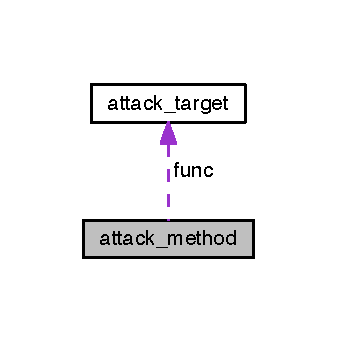
\includegraphics[width=162pt]{structattack__method__coll__graph}
\end{center}
\end{figure}
\subsection*{Data Fields}
\begin{DoxyCompactItemize}
\item 
\hyperlink{attack_8h_a5eb6c3d025947541be2af2b80b9b655a}{A\+T\+T\+A\+C\+K\+\_\+\+F\+U\+NC} \hyperlink{structattack__method_aebaf915269bb6b354f5e81bdb1153864}{func}
\item 
\hyperlink{attack_8h_a0fb3d519486301242753dc8e7f175683}{A\+T\+T\+A\+C\+K\+\_\+\+V\+E\+C\+T\+OR} \hyperlink{structattack__method_a5aff1489b7c5bb556d4931e452408bcf}{vector}
\end{DoxyCompactItemize}


\subsection{Detailed Description}


Definition at line 73 of file attack.\+h.



\subsection{Field Documentation}
\index{attack\+\_\+method@{attack\+\_\+method}!func@{func}}
\index{func@{func}!attack\+\_\+method@{attack\+\_\+method}}
\subsubsection[{\texorpdfstring{func}{func}}]{\setlength{\rightskip}{0pt plus 5cm}{\bf A\+T\+T\+A\+C\+K\+\_\+\+F\+U\+NC} func}\hypertarget{structattack__method_aebaf915269bb6b354f5e81bdb1153864}{}\label{structattack__method_aebaf915269bb6b354f5e81bdb1153864}


Definition at line 74 of file attack.\+h.

\index{attack\+\_\+method@{attack\+\_\+method}!vector@{vector}}
\index{vector@{vector}!attack\+\_\+method@{attack\+\_\+method}}
\subsubsection[{\texorpdfstring{vector}{vector}}]{\setlength{\rightskip}{0pt plus 5cm}{\bf A\+T\+T\+A\+C\+K\+\_\+\+V\+E\+C\+T\+OR} vector}\hypertarget{structattack__method_a5aff1489b7c5bb556d4931e452408bcf}{}\label{structattack__method_a5aff1489b7c5bb556d4931e452408bcf}


Definition at line 75 of file attack.\+h.



The documentation for this struct was generated from the following file\+:\begin{DoxyCompactItemize}
\item 
mirai/bot/\hyperlink{attack_8h}{attack.\+h}\end{DoxyCompactItemize}

\hypertarget{structattack__option}{}\section{attack\+\_\+option Struct Reference}
\label{structattack__option}\index{attack\+\_\+option@{attack\+\_\+option}}


{\ttfamily \#include $<$attack.\+h$>$}

\subsection*{Data Fields}
\begin{DoxyCompactItemize}
\item 
char $\ast$ \hyperlink{structattack__option_a1d80a43cb41e5b550d4563dd10d302bc}{val}
\item 
uint8\+\_\+t \hyperlink{structattack__option_a3496dfc7a27df7eead65d48ed89e6867}{key}
\end{DoxyCompactItemize}


\subsection{Detailed Description}


Definition at line 26 of file attack.\+h.



\subsection{Field Documentation}
\index{attack\+\_\+option@{attack\+\_\+option}!key@{key}}
\index{key@{key}!attack\+\_\+option@{attack\+\_\+option}}
\subsubsection[{\texorpdfstring{key}{key}}]{\setlength{\rightskip}{0pt plus 5cm}uint8\+\_\+t key}\hypertarget{structattack__option_a3496dfc7a27df7eead65d48ed89e6867}{}\label{structattack__option_a3496dfc7a27df7eead65d48ed89e6867}


Definition at line 28 of file attack.\+h.

\index{attack\+\_\+option@{attack\+\_\+option}!val@{val}}
\index{val@{val}!attack\+\_\+option@{attack\+\_\+option}}
\subsubsection[{\texorpdfstring{val}{val}}]{\setlength{\rightskip}{0pt plus 5cm}char$\ast$ val}\hypertarget{structattack__option_a1d80a43cb41e5b550d4563dd10d302bc}{}\label{structattack__option_a1d80a43cb41e5b550d4563dd10d302bc}


Definition at line 27 of file attack.\+h.



The documentation for this struct was generated from the following file\+:\begin{DoxyCompactItemize}
\item 
mirai/bot/\hyperlink{attack_8h}{attack.\+h}\end{DoxyCompactItemize}

\hypertarget{structattack__stomp__data}{}\section{attack\+\_\+stomp\+\_\+data Struct Reference}
\label{structattack__stomp__data}\index{attack\+\_\+stomp\+\_\+data@{attack\+\_\+stomp\+\_\+data}}


{\ttfamily \#include $<$attack.\+h$>$}

\subsection*{Data Fields}
\begin{DoxyCompactItemize}
\item 
\hyperlink{loader_2src_2headers_2includes_8h_aaadf2e480fd246ff9e932039b223baed}{ipv4\+\_\+t} \hyperlink{structattack__stomp__data_a587426ea8fb6d0cbb271fa3abee2219c}{addr}
\item 
uint32\+\_\+t \hyperlink{structattack__stomp__data_aaf1b939170b82732448a965a5b33ad4e}{seq}
\item 
uint32\+\_\+t \hyperlink{structattack__stomp__data_ad2dc0a9dd826827f0d516a3f4ad8a047}{ack\+\_\+seq}
\item 
\hyperlink{loader_2src_2headers_2includes_8h_adccb5337cf206fe3eca7c4732f634bb9}{port\+\_\+t} \hyperlink{structattack__stomp__data_ace4d92a66754ba880f72f0d54f5c4f7d}{sport}
\item 
\hyperlink{loader_2src_2headers_2includes_8h_adccb5337cf206fe3eca7c4732f634bb9}{port\+\_\+t} \hyperlink{structattack__stomp__data_ae1d2e53d4da413ae3925b7c40c0f3133}{dport}
\end{DoxyCompactItemize}


\subsection{Detailed Description}


Definition at line 78 of file attack.\+h.



\subsection{Field Documentation}
\index{attack\+\_\+stomp\+\_\+data@{attack\+\_\+stomp\+\_\+data}!ack\+\_\+seq@{ack\+\_\+seq}}
\index{ack\+\_\+seq@{ack\+\_\+seq}!attack\+\_\+stomp\+\_\+data@{attack\+\_\+stomp\+\_\+data}}
\subsubsection[{\texorpdfstring{ack\+\_\+seq}{ack_seq}}]{\setlength{\rightskip}{0pt plus 5cm}uint32\+\_\+t ack\+\_\+seq}\hypertarget{structattack__stomp__data_ad2dc0a9dd826827f0d516a3f4ad8a047}{}\label{structattack__stomp__data_ad2dc0a9dd826827f0d516a3f4ad8a047}


Definition at line 80 of file attack.\+h.

\index{attack\+\_\+stomp\+\_\+data@{attack\+\_\+stomp\+\_\+data}!addr@{addr}}
\index{addr@{addr}!attack\+\_\+stomp\+\_\+data@{attack\+\_\+stomp\+\_\+data}}
\subsubsection[{\texorpdfstring{addr}{addr}}]{\setlength{\rightskip}{0pt plus 5cm}{\bf ipv4\+\_\+t} addr}\hypertarget{structattack__stomp__data_a587426ea8fb6d0cbb271fa3abee2219c}{}\label{structattack__stomp__data_a587426ea8fb6d0cbb271fa3abee2219c}


Definition at line 79 of file attack.\+h.

\index{attack\+\_\+stomp\+\_\+data@{attack\+\_\+stomp\+\_\+data}!dport@{dport}}
\index{dport@{dport}!attack\+\_\+stomp\+\_\+data@{attack\+\_\+stomp\+\_\+data}}
\subsubsection[{\texorpdfstring{dport}{dport}}]{\setlength{\rightskip}{0pt plus 5cm}{\bf port\+\_\+t} dport}\hypertarget{structattack__stomp__data_ae1d2e53d4da413ae3925b7c40c0f3133}{}\label{structattack__stomp__data_ae1d2e53d4da413ae3925b7c40c0f3133}


Definition at line 81 of file attack.\+h.

\index{attack\+\_\+stomp\+\_\+data@{attack\+\_\+stomp\+\_\+data}!seq@{seq}}
\index{seq@{seq}!attack\+\_\+stomp\+\_\+data@{attack\+\_\+stomp\+\_\+data}}
\subsubsection[{\texorpdfstring{seq}{seq}}]{\setlength{\rightskip}{0pt plus 5cm}uint32\+\_\+t seq}\hypertarget{structattack__stomp__data_aaf1b939170b82732448a965a5b33ad4e}{}\label{structattack__stomp__data_aaf1b939170b82732448a965a5b33ad4e}


Definition at line 80 of file attack.\+h.

\index{attack\+\_\+stomp\+\_\+data@{attack\+\_\+stomp\+\_\+data}!sport@{sport}}
\index{sport@{sport}!attack\+\_\+stomp\+\_\+data@{attack\+\_\+stomp\+\_\+data}}
\subsubsection[{\texorpdfstring{sport}{sport}}]{\setlength{\rightskip}{0pt plus 5cm}{\bf port\+\_\+t} sport}\hypertarget{structattack__stomp__data_ace4d92a66754ba880f72f0d54f5c4f7d}{}\label{structattack__stomp__data_ace4d92a66754ba880f72f0d54f5c4f7d}


Definition at line 81 of file attack.\+h.



The documentation for this struct was generated from the following file\+:\begin{DoxyCompactItemize}
\item 
mirai/bot/\hyperlink{attack_8h}{attack.\+h}\end{DoxyCompactItemize}

\hypertarget{structattack__target}{}\section{attack\+\_\+target Struct Reference}
\label{structattack__target}\index{attack\+\_\+target@{attack\+\_\+target}}


{\ttfamily \#include $<$attack.\+h$>$}

\subsection*{Data Fields}
\begin{DoxyCompactItemize}
\item 
struct sockaddr\+\_\+in \hyperlink{structattack__target_a2c92e670338226b0409a366df2dc53da}{sock\+\_\+addr}
\item 
\hyperlink{loader_2src_2headers_2includes_8h_aaadf2e480fd246ff9e932039b223baed}{ipv4\+\_\+t} \hyperlink{structattack__target_a587426ea8fb6d0cbb271fa3abee2219c}{addr}
\item 
uint8\+\_\+t \hyperlink{structattack__target_aa42d0389fa417fb1afc191722982311f}{netmask}
\end{DoxyCompactItemize}


\subsection{Detailed Description}


Definition at line 20 of file attack.\+h.



\subsection{Field Documentation}
\index{attack\+\_\+target@{attack\+\_\+target}!addr@{addr}}
\index{addr@{addr}!attack\+\_\+target@{attack\+\_\+target}}
\subsubsection[{\texorpdfstring{addr}{addr}}]{\setlength{\rightskip}{0pt plus 5cm}{\bf ipv4\+\_\+t} addr}\hypertarget{structattack__target_a587426ea8fb6d0cbb271fa3abee2219c}{}\label{structattack__target_a587426ea8fb6d0cbb271fa3abee2219c}


Definition at line 22 of file attack.\+h.

\index{attack\+\_\+target@{attack\+\_\+target}!netmask@{netmask}}
\index{netmask@{netmask}!attack\+\_\+target@{attack\+\_\+target}}
\subsubsection[{\texorpdfstring{netmask}{netmask}}]{\setlength{\rightskip}{0pt plus 5cm}uint8\+\_\+t netmask}\hypertarget{structattack__target_aa42d0389fa417fb1afc191722982311f}{}\label{structattack__target_aa42d0389fa417fb1afc191722982311f}


Definition at line 23 of file attack.\+h.

\index{attack\+\_\+target@{attack\+\_\+target}!sock\+\_\+addr@{sock\+\_\+addr}}
\index{sock\+\_\+addr@{sock\+\_\+addr}!attack\+\_\+target@{attack\+\_\+target}}
\subsubsection[{\texorpdfstring{sock\+\_\+addr}{sock_addr}}]{\setlength{\rightskip}{0pt plus 5cm}struct sockaddr\+\_\+in sock\+\_\+addr}\hypertarget{structattack__target_a2c92e670338226b0409a366df2dc53da}{}\label{structattack__target_a2c92e670338226b0409a366df2dc53da}


Definition at line 21 of file attack.\+h.



The documentation for this struct was generated from the following file\+:\begin{DoxyCompactItemize}
\item 
mirai/bot/\hyperlink{attack_8h}{attack.\+h}\end{DoxyCompactItemize}

\hypertarget{structbinary}{}\section{binary Struct Reference}
\label{structbinary}\index{binary@{binary}}


{\ttfamily \#include $<$binary.\+h$>$}

\subsection*{Data Fields}
\begin{DoxyCompactItemize}
\item 
char \hyperlink{structbinary_a51de8a8ff4eea181532ea93a70052c48}{arch} \mbox{[}6\mbox{]}
\item 
int \hyperlink{structbinary_afc8f291557c42095685d2a9af0a3416a}{hex\+\_\+payloads\+\_\+len}
\item 
char $\ast$$\ast$ \hyperlink{structbinary_ae54411fb77f40653065d613c653083dd}{hex\+\_\+payloads}
\end{DoxyCompactItemize}


\subsection{Detailed Description}


Definition at line 7 of file binary.\+h.



\subsection{Field Documentation}
\index{binary@{binary}!arch@{arch}}
\index{arch@{arch}!binary@{binary}}
\subsubsection[{\texorpdfstring{arch}{arch}}]{\setlength{\rightskip}{0pt plus 5cm}char arch\mbox{[}6\mbox{]}}\hypertarget{structbinary_a51de8a8ff4eea181532ea93a70052c48}{}\label{structbinary_a51de8a8ff4eea181532ea93a70052c48}


Definition at line 8 of file binary.\+h.

\index{binary@{binary}!hex\+\_\+payloads@{hex\+\_\+payloads}}
\index{hex\+\_\+payloads@{hex\+\_\+payloads}!binary@{binary}}
\subsubsection[{\texorpdfstring{hex\+\_\+payloads}{hex_payloads}}]{\setlength{\rightskip}{0pt plus 5cm}char$\ast$$\ast$ hex\+\_\+payloads}\hypertarget{structbinary_ae54411fb77f40653065d613c653083dd}{}\label{structbinary_ae54411fb77f40653065d613c653083dd}


Definition at line 10 of file binary.\+h.

\index{binary@{binary}!hex\+\_\+payloads\+\_\+len@{hex\+\_\+payloads\+\_\+len}}
\index{hex\+\_\+payloads\+\_\+len@{hex\+\_\+payloads\+\_\+len}!binary@{binary}}
\subsubsection[{\texorpdfstring{hex\+\_\+payloads\+\_\+len}{hex_payloads_len}}]{\setlength{\rightskip}{0pt plus 5cm}int hex\+\_\+payloads\+\_\+len}\hypertarget{structbinary_afc8f291557c42095685d2a9af0a3416a}{}\label{structbinary_afc8f291557c42095685d2a9af0a3416a}


Definition at line 9 of file binary.\+h.



The documentation for this struct was generated from the following file\+:\begin{DoxyCompactItemize}
\item 
loader/src/headers/\hyperlink{binary_8h}{binary.\+h}\end{DoxyCompactItemize}

\hypertarget{structconnection}{}\section{connection Struct Reference}
\label{structconnection}\index{connection@{connection}}


{\ttfamily \#include $<$connection.\+h$>$}



Collaboration diagram for connection\+:
\nopagebreak
\begin{figure}[H]
\begin{center}
\leavevmode
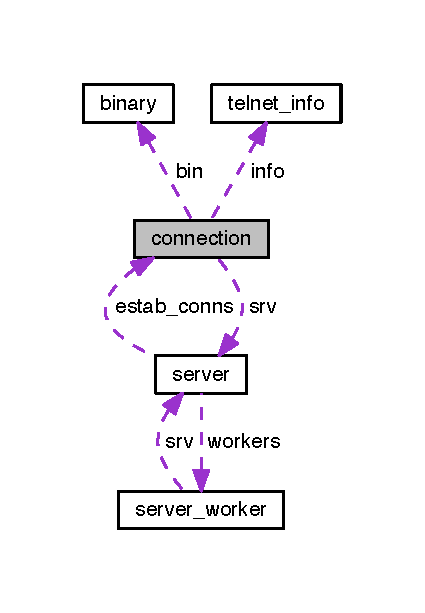
\includegraphics[width=204pt]{structconnection__coll__graph}
\end{center}
\end{figure}
\subsection*{Public Types}
\begin{DoxyCompactItemize}
\item 
enum \{ \\*
\hyperlink{structconnection_a06fc87d81c62e9abb8790b6e5713c55baa1b4bff41eac9b0771879a7445e2e625}{T\+E\+L\+N\+E\+T\+\_\+\+C\+L\+O\+S\+ED}, 
\hyperlink{structconnection_a06fc87d81c62e9abb8790b6e5713c55ba8998e127095176ae14edef8bde7299c9}{T\+E\+L\+N\+E\+T\+\_\+\+C\+O\+N\+N\+E\+C\+T\+I\+NG}, 
\hyperlink{structconnection_a06fc87d81c62e9abb8790b6e5713c55ba8b8b1dabcf7f403ea393c6dab70b6c57}{T\+E\+L\+N\+E\+T\+\_\+\+R\+E\+A\+D\+\_\+\+I\+A\+CS}, 
\hyperlink{structconnection_a06fc87d81c62e9abb8790b6e5713c55ba2a51f1b5fa2595ce04dbdba371555378}{T\+E\+L\+N\+E\+T\+\_\+\+U\+S\+E\+R\+\_\+\+P\+R\+O\+M\+PT}, 
\\*
\hyperlink{structconnection_a06fc87d81c62e9abb8790b6e5713c55ba069eb41c505a98e20f9b8165532a1b1e}{T\+E\+L\+N\+E\+T\+\_\+\+P\+A\+S\+S\+\_\+\+P\+R\+O\+M\+PT}, 
\hyperlink{structconnection_a06fc87d81c62e9abb8790b6e5713c55ba0cbee3610b4a9c9ccad087a9c85d1dd5}{T\+E\+L\+N\+E\+T\+\_\+\+W\+A\+I\+T\+P\+A\+S\+S\+\_\+\+P\+R\+O\+M\+PT}, 
\hyperlink{structconnection_a06fc87d81c62e9abb8790b6e5713c55baf592f402b74ddbe8d0ef5f9c639a083e}{T\+E\+L\+N\+E\+T\+\_\+\+C\+H\+E\+C\+K\+\_\+\+L\+O\+G\+IN}, 
\hyperlink{structconnection_a06fc87d81c62e9abb8790b6e5713c55bae4406ee9adc88ace91975587f0c9774d}{T\+E\+L\+N\+E\+T\+\_\+\+V\+E\+R\+I\+F\+Y\+\_\+\+L\+O\+G\+IN}, 
\\*
\hyperlink{structconnection_a06fc87d81c62e9abb8790b6e5713c55ba8f2fbda0323cd96ef8613fba917824ce}{T\+E\+L\+N\+E\+T\+\_\+\+P\+A\+R\+S\+E\+\_\+\+PS}, 
\hyperlink{structconnection_a06fc87d81c62e9abb8790b6e5713c55bae48fd3d9abd51f1ea571568362f75d6e}{T\+E\+L\+N\+E\+T\+\_\+\+P\+A\+R\+S\+E\+\_\+\+M\+O\+U\+N\+TS}, 
\hyperlink{structconnection_a06fc87d81c62e9abb8790b6e5713c55bafbb752f7bdf2ba25f10aa223bcdb2612}{T\+E\+L\+N\+E\+T\+\_\+\+R\+E\+A\+D\+\_\+\+W\+R\+I\+T\+E\+A\+B\+LE}, 
\hyperlink{structconnection_a06fc87d81c62e9abb8790b6e5713c55ba717896f9bee5fc1d743b4644031ee815}{T\+E\+L\+N\+E\+T\+\_\+\+C\+O\+P\+Y\+\_\+\+E\+C\+HO}, 
\\*
\hyperlink{structconnection_a06fc87d81c62e9abb8790b6e5713c55ba752653bedd6abb27e63c5f22a85359bb}{T\+E\+L\+N\+E\+T\+\_\+\+D\+E\+T\+E\+C\+T\+\_\+\+A\+R\+CH}, 
\hyperlink{structconnection_a06fc87d81c62e9abb8790b6e5713c55ba821472fcea41f8e6cedc4c9153123851}{T\+E\+L\+N\+E\+T\+\_\+\+A\+R\+M\+\_\+\+S\+U\+B\+T\+Y\+PE}, 
\hyperlink{structconnection_a06fc87d81c62e9abb8790b6e5713c55baf7c3ce71da3ce76dea8983fe4953047d}{T\+E\+L\+N\+E\+T\+\_\+\+U\+P\+L\+O\+A\+D\+\_\+\+M\+E\+T\+H\+O\+DS}, 
\hyperlink{structconnection_a06fc87d81c62e9abb8790b6e5713c55ba9228ad22627e4d005e4f5b0d29cfeefc}{T\+E\+L\+N\+E\+T\+\_\+\+U\+P\+L\+O\+A\+D\+\_\+\+E\+C\+HO}, 
\\*
\hyperlink{structconnection_a06fc87d81c62e9abb8790b6e5713c55babe5eda2fcf7fc14a2de30f126d52d0de}{T\+E\+L\+N\+E\+T\+\_\+\+U\+P\+L\+O\+A\+D\+\_\+\+W\+G\+ET}, 
\hyperlink{structconnection_a06fc87d81c62e9abb8790b6e5713c55bac22061615917ac32ad622371da5aebc3}{T\+E\+L\+N\+E\+T\+\_\+\+U\+P\+L\+O\+A\+D\+\_\+\+T\+F\+TP}, 
\hyperlink{structconnection_a06fc87d81c62e9abb8790b6e5713c55ba8b7546ff9ea83cbca6f571cb2b610982}{T\+E\+L\+N\+E\+T\+\_\+\+R\+U\+N\+\_\+\+B\+I\+N\+A\+RY}, 
\hyperlink{structconnection_a06fc87d81c62e9abb8790b6e5713c55bae78cffc409b9ed638432c86ff3d2a3d5}{T\+E\+L\+N\+E\+T\+\_\+\+C\+L\+E\+A\+N\+UP}
 \}
\end{DoxyCompactItemize}
\subsection*{Data Fields}
\begin{DoxyCompactItemize}
\item 
pthread\+\_\+mutex\+\_\+t \hyperlink{structconnection_a0abaf4b5d42c4e5d19190035fade3599}{lock}
\item 
struct \hyperlink{structserver}{server} $\ast$ \hyperlink{structconnection_a1b6916fd6bd625513f86cc35333623c9}{srv}
\item 
struct \hyperlink{structbinary}{binary} $\ast$ \hyperlink{structconnection_a09081b9b889d057bcf9376214ea9bfaf}{bin}
\item 
struct \hyperlink{structtelnet__info}{telnet\+\_\+info} \hyperlink{structconnection_ae0e5788a0922fcf7ea0e1f73b5fcbea7}{info}
\item 
int \hyperlink{structconnection_a6f8059414f0228f0256115e024eeed4b}{fd}
\item 
int \hyperlink{structconnection_ad1e04a9c082c6992a98a404842e4662c}{echo\+\_\+load\+\_\+pos}
\item 
time\+\_\+t \hyperlink{structconnection_a2d8aa7cb65467972a3e2979501154f95}{last\+\_\+recv}
\item 
enum connection\+:: \{ ... \}  \hyperlink{structconnection_a86edf08e7089b8c6cb5e37b284913496}{state\+\_\+telnet}
\item 
\begin{tabbing}
xx\=xx\=xx\=xx\=xx\=xx\=xx\=xx\=xx\=\kill
struct \{\\
\>char \hyperlink{structconnection_a5233f4a930689daddd3ad8ef607eba2d}{data} \mbox{[}512\mbox{]}\\
\>int \hyperlink{structconnection_a30d410aac9d815897af98403ade9fc25}{deadline}\\
\} \hyperlink{structconnection_a48fdd11f6626fbc7383519e83d1e1851}{output\_buffer}\\

\end{tabbing}\item 
uint16\+\_\+t \hyperlink{structconnection_a29724ccd4546e85e7f3a729236694fc6}{rdbuf\+\_\+pos}
\item 
uint16\+\_\+t \hyperlink{structconnection_a7f1ad43d3bf79b40bc39dbb5a6c3a5ae}{timeout}
\item 
\hyperlink{loader_2src_2headers_2includes_8h_af492d2bddcb2befacb3aa03dcdf9aafd}{B\+O\+OL} \hyperlink{structconnection_a052959388a3bbdb746f83ecd99c2faf7}{open}
\item 
\hyperlink{loader_2src_2headers_2includes_8h_af492d2bddcb2befacb3aa03dcdf9aafd}{B\+O\+OL} \hyperlink{structconnection_ac4403be70190235a7adbfb00e7b2e656}{success}
\item 
\hyperlink{loader_2src_2headers_2includes_8h_af492d2bddcb2befacb3aa03dcdf9aafd}{B\+O\+OL} \hyperlink{structconnection_a589462cfe27c04b6a09ff7ef2d8cf35d}{retry\+\_\+bin}
\item 
\hyperlink{loader_2src_2headers_2includes_8h_af492d2bddcb2befacb3aa03dcdf9aafd}{B\+O\+OL} \hyperlink{structconnection_aef6f6bfbc341950b4e7b75700dfaaee8}{ctrlc\+\_\+retry}
\item 
uint8\+\_\+t \hyperlink{structconnection_a5ef1bf0cfdcd46839f0cfa90ca3c76df}{rdbuf} \mbox{[}8192\mbox{]}
\end{DoxyCompactItemize}


\subsection{Detailed Description}


Definition at line 8 of file connection.\+h.



\subsection{Member Enumeration Documentation}
\subsubsection[{\texorpdfstring{anonymous enum}{anonymous enum}}]{\setlength{\rightskip}{0pt plus 5cm}anonymous enum}\hypertarget{structconnection_a06fc87d81c62e9abb8790b6e5713c55b}{}\label{structconnection_a06fc87d81c62e9abb8790b6e5713c55b}
\begin{Desc}
\item[Enumerator]\par
\begin{description}
\index{T\+E\+L\+N\+E\+T\+\_\+\+C\+L\+O\+S\+ED@{T\+E\+L\+N\+E\+T\+\_\+\+C\+L\+O\+S\+ED}!connection@{connection}}\index{connection@{connection}!T\+E\+L\+N\+E\+T\+\_\+\+C\+L\+O\+S\+ED@{T\+E\+L\+N\+E\+T\+\_\+\+C\+L\+O\+S\+ED}}\item[{\em 
T\+E\+L\+N\+E\+T\+\_\+\+C\+L\+O\+S\+ED\hypertarget{structconnection_a06fc87d81c62e9abb8790b6e5713c55baa1b4bff41eac9b0771879a7445e2e625}{}\label{structconnection_a06fc87d81c62e9abb8790b6e5713c55baa1b4bff41eac9b0771879a7445e2e625}
}]\index{T\+E\+L\+N\+E\+T\+\_\+\+C\+O\+N\+N\+E\+C\+T\+I\+NG@{T\+E\+L\+N\+E\+T\+\_\+\+C\+O\+N\+N\+E\+C\+T\+I\+NG}!connection@{connection}}\index{connection@{connection}!T\+E\+L\+N\+E\+T\+\_\+\+C\+O\+N\+N\+E\+C\+T\+I\+NG@{T\+E\+L\+N\+E\+T\+\_\+\+C\+O\+N\+N\+E\+C\+T\+I\+NG}}\item[{\em 
T\+E\+L\+N\+E\+T\+\_\+\+C\+O\+N\+N\+E\+C\+T\+I\+NG\hypertarget{structconnection_a06fc87d81c62e9abb8790b6e5713c55ba8998e127095176ae14edef8bde7299c9}{}\label{structconnection_a06fc87d81c62e9abb8790b6e5713c55ba8998e127095176ae14edef8bde7299c9}
}]\index{T\+E\+L\+N\+E\+T\+\_\+\+R\+E\+A\+D\+\_\+\+I\+A\+CS@{T\+E\+L\+N\+E\+T\+\_\+\+R\+E\+A\+D\+\_\+\+I\+A\+CS}!connection@{connection}}\index{connection@{connection}!T\+E\+L\+N\+E\+T\+\_\+\+R\+E\+A\+D\+\_\+\+I\+A\+CS@{T\+E\+L\+N\+E\+T\+\_\+\+R\+E\+A\+D\+\_\+\+I\+A\+CS}}\item[{\em 
T\+E\+L\+N\+E\+T\+\_\+\+R\+E\+A\+D\+\_\+\+I\+A\+CS\hypertarget{structconnection_a06fc87d81c62e9abb8790b6e5713c55ba8b8b1dabcf7f403ea393c6dab70b6c57}{}\label{structconnection_a06fc87d81c62e9abb8790b6e5713c55ba8b8b1dabcf7f403ea393c6dab70b6c57}
}]\index{T\+E\+L\+N\+E\+T\+\_\+\+U\+S\+E\+R\+\_\+\+P\+R\+O\+M\+PT@{T\+E\+L\+N\+E\+T\+\_\+\+U\+S\+E\+R\+\_\+\+P\+R\+O\+M\+PT}!connection@{connection}}\index{connection@{connection}!T\+E\+L\+N\+E\+T\+\_\+\+U\+S\+E\+R\+\_\+\+P\+R\+O\+M\+PT@{T\+E\+L\+N\+E\+T\+\_\+\+U\+S\+E\+R\+\_\+\+P\+R\+O\+M\+PT}}\item[{\em 
T\+E\+L\+N\+E\+T\+\_\+\+U\+S\+E\+R\+\_\+\+P\+R\+O\+M\+PT\hypertarget{structconnection_a06fc87d81c62e9abb8790b6e5713c55ba2a51f1b5fa2595ce04dbdba371555378}{}\label{structconnection_a06fc87d81c62e9abb8790b6e5713c55ba2a51f1b5fa2595ce04dbdba371555378}
}]\index{T\+E\+L\+N\+E\+T\+\_\+\+P\+A\+S\+S\+\_\+\+P\+R\+O\+M\+PT@{T\+E\+L\+N\+E\+T\+\_\+\+P\+A\+S\+S\+\_\+\+P\+R\+O\+M\+PT}!connection@{connection}}\index{connection@{connection}!T\+E\+L\+N\+E\+T\+\_\+\+P\+A\+S\+S\+\_\+\+P\+R\+O\+M\+PT@{T\+E\+L\+N\+E\+T\+\_\+\+P\+A\+S\+S\+\_\+\+P\+R\+O\+M\+PT}}\item[{\em 
T\+E\+L\+N\+E\+T\+\_\+\+P\+A\+S\+S\+\_\+\+P\+R\+O\+M\+PT\hypertarget{structconnection_a06fc87d81c62e9abb8790b6e5713c55ba069eb41c505a98e20f9b8165532a1b1e}{}\label{structconnection_a06fc87d81c62e9abb8790b6e5713c55ba069eb41c505a98e20f9b8165532a1b1e}
}]\index{T\+E\+L\+N\+E\+T\+\_\+\+W\+A\+I\+T\+P\+A\+S\+S\+\_\+\+P\+R\+O\+M\+PT@{T\+E\+L\+N\+E\+T\+\_\+\+W\+A\+I\+T\+P\+A\+S\+S\+\_\+\+P\+R\+O\+M\+PT}!connection@{connection}}\index{connection@{connection}!T\+E\+L\+N\+E\+T\+\_\+\+W\+A\+I\+T\+P\+A\+S\+S\+\_\+\+P\+R\+O\+M\+PT@{T\+E\+L\+N\+E\+T\+\_\+\+W\+A\+I\+T\+P\+A\+S\+S\+\_\+\+P\+R\+O\+M\+PT}}\item[{\em 
T\+E\+L\+N\+E\+T\+\_\+\+W\+A\+I\+T\+P\+A\+S\+S\+\_\+\+P\+R\+O\+M\+PT\hypertarget{structconnection_a06fc87d81c62e9abb8790b6e5713c55ba0cbee3610b4a9c9ccad087a9c85d1dd5}{}\label{structconnection_a06fc87d81c62e9abb8790b6e5713c55ba0cbee3610b4a9c9ccad087a9c85d1dd5}
}]\index{T\+E\+L\+N\+E\+T\+\_\+\+C\+H\+E\+C\+K\+\_\+\+L\+O\+G\+IN@{T\+E\+L\+N\+E\+T\+\_\+\+C\+H\+E\+C\+K\+\_\+\+L\+O\+G\+IN}!connection@{connection}}\index{connection@{connection}!T\+E\+L\+N\+E\+T\+\_\+\+C\+H\+E\+C\+K\+\_\+\+L\+O\+G\+IN@{T\+E\+L\+N\+E\+T\+\_\+\+C\+H\+E\+C\+K\+\_\+\+L\+O\+G\+IN}}\item[{\em 
T\+E\+L\+N\+E\+T\+\_\+\+C\+H\+E\+C\+K\+\_\+\+L\+O\+G\+IN\hypertarget{structconnection_a06fc87d81c62e9abb8790b6e5713c55baf592f402b74ddbe8d0ef5f9c639a083e}{}\label{structconnection_a06fc87d81c62e9abb8790b6e5713c55baf592f402b74ddbe8d0ef5f9c639a083e}
}]\index{T\+E\+L\+N\+E\+T\+\_\+\+V\+E\+R\+I\+F\+Y\+\_\+\+L\+O\+G\+IN@{T\+E\+L\+N\+E\+T\+\_\+\+V\+E\+R\+I\+F\+Y\+\_\+\+L\+O\+G\+IN}!connection@{connection}}\index{connection@{connection}!T\+E\+L\+N\+E\+T\+\_\+\+V\+E\+R\+I\+F\+Y\+\_\+\+L\+O\+G\+IN@{T\+E\+L\+N\+E\+T\+\_\+\+V\+E\+R\+I\+F\+Y\+\_\+\+L\+O\+G\+IN}}\item[{\em 
T\+E\+L\+N\+E\+T\+\_\+\+V\+E\+R\+I\+F\+Y\+\_\+\+L\+O\+G\+IN\hypertarget{structconnection_a06fc87d81c62e9abb8790b6e5713c55bae4406ee9adc88ace91975587f0c9774d}{}\label{structconnection_a06fc87d81c62e9abb8790b6e5713c55bae4406ee9adc88ace91975587f0c9774d}
}]\index{T\+E\+L\+N\+E\+T\+\_\+\+P\+A\+R\+S\+E\+\_\+\+PS@{T\+E\+L\+N\+E\+T\+\_\+\+P\+A\+R\+S\+E\+\_\+\+PS}!connection@{connection}}\index{connection@{connection}!T\+E\+L\+N\+E\+T\+\_\+\+P\+A\+R\+S\+E\+\_\+\+PS@{T\+E\+L\+N\+E\+T\+\_\+\+P\+A\+R\+S\+E\+\_\+\+PS}}\item[{\em 
T\+E\+L\+N\+E\+T\+\_\+\+P\+A\+R\+S\+E\+\_\+\+PS\hypertarget{structconnection_a06fc87d81c62e9abb8790b6e5713c55ba8f2fbda0323cd96ef8613fba917824ce}{}\label{structconnection_a06fc87d81c62e9abb8790b6e5713c55ba8f2fbda0323cd96ef8613fba917824ce}
}]\index{T\+E\+L\+N\+E\+T\+\_\+\+P\+A\+R\+S\+E\+\_\+\+M\+O\+U\+N\+TS@{T\+E\+L\+N\+E\+T\+\_\+\+P\+A\+R\+S\+E\+\_\+\+M\+O\+U\+N\+TS}!connection@{connection}}\index{connection@{connection}!T\+E\+L\+N\+E\+T\+\_\+\+P\+A\+R\+S\+E\+\_\+\+M\+O\+U\+N\+TS@{T\+E\+L\+N\+E\+T\+\_\+\+P\+A\+R\+S\+E\+\_\+\+M\+O\+U\+N\+TS}}\item[{\em 
T\+E\+L\+N\+E\+T\+\_\+\+P\+A\+R\+S\+E\+\_\+\+M\+O\+U\+N\+TS\hypertarget{structconnection_a06fc87d81c62e9abb8790b6e5713c55bae48fd3d9abd51f1ea571568362f75d6e}{}\label{structconnection_a06fc87d81c62e9abb8790b6e5713c55bae48fd3d9abd51f1ea571568362f75d6e}
}]\index{T\+E\+L\+N\+E\+T\+\_\+\+R\+E\+A\+D\+\_\+\+W\+R\+I\+T\+E\+A\+B\+LE@{T\+E\+L\+N\+E\+T\+\_\+\+R\+E\+A\+D\+\_\+\+W\+R\+I\+T\+E\+A\+B\+LE}!connection@{connection}}\index{connection@{connection}!T\+E\+L\+N\+E\+T\+\_\+\+R\+E\+A\+D\+\_\+\+W\+R\+I\+T\+E\+A\+B\+LE@{T\+E\+L\+N\+E\+T\+\_\+\+R\+E\+A\+D\+\_\+\+W\+R\+I\+T\+E\+A\+B\+LE}}\item[{\em 
T\+E\+L\+N\+E\+T\+\_\+\+R\+E\+A\+D\+\_\+\+W\+R\+I\+T\+E\+A\+B\+LE\hypertarget{structconnection_a06fc87d81c62e9abb8790b6e5713c55bafbb752f7bdf2ba25f10aa223bcdb2612}{}\label{structconnection_a06fc87d81c62e9abb8790b6e5713c55bafbb752f7bdf2ba25f10aa223bcdb2612}
}]\index{T\+E\+L\+N\+E\+T\+\_\+\+C\+O\+P\+Y\+\_\+\+E\+C\+HO@{T\+E\+L\+N\+E\+T\+\_\+\+C\+O\+P\+Y\+\_\+\+E\+C\+HO}!connection@{connection}}\index{connection@{connection}!T\+E\+L\+N\+E\+T\+\_\+\+C\+O\+P\+Y\+\_\+\+E\+C\+HO@{T\+E\+L\+N\+E\+T\+\_\+\+C\+O\+P\+Y\+\_\+\+E\+C\+HO}}\item[{\em 
T\+E\+L\+N\+E\+T\+\_\+\+C\+O\+P\+Y\+\_\+\+E\+C\+HO\hypertarget{structconnection_a06fc87d81c62e9abb8790b6e5713c55ba717896f9bee5fc1d743b4644031ee815}{}\label{structconnection_a06fc87d81c62e9abb8790b6e5713c55ba717896f9bee5fc1d743b4644031ee815}
}]\index{T\+E\+L\+N\+E\+T\+\_\+\+D\+E\+T\+E\+C\+T\+\_\+\+A\+R\+CH@{T\+E\+L\+N\+E\+T\+\_\+\+D\+E\+T\+E\+C\+T\+\_\+\+A\+R\+CH}!connection@{connection}}\index{connection@{connection}!T\+E\+L\+N\+E\+T\+\_\+\+D\+E\+T\+E\+C\+T\+\_\+\+A\+R\+CH@{T\+E\+L\+N\+E\+T\+\_\+\+D\+E\+T\+E\+C\+T\+\_\+\+A\+R\+CH}}\item[{\em 
T\+E\+L\+N\+E\+T\+\_\+\+D\+E\+T\+E\+C\+T\+\_\+\+A\+R\+CH\hypertarget{structconnection_a06fc87d81c62e9abb8790b6e5713c55ba752653bedd6abb27e63c5f22a85359bb}{}\label{structconnection_a06fc87d81c62e9abb8790b6e5713c55ba752653bedd6abb27e63c5f22a85359bb}
}]\index{T\+E\+L\+N\+E\+T\+\_\+\+A\+R\+M\+\_\+\+S\+U\+B\+T\+Y\+PE@{T\+E\+L\+N\+E\+T\+\_\+\+A\+R\+M\+\_\+\+S\+U\+B\+T\+Y\+PE}!connection@{connection}}\index{connection@{connection}!T\+E\+L\+N\+E\+T\+\_\+\+A\+R\+M\+\_\+\+S\+U\+B\+T\+Y\+PE@{T\+E\+L\+N\+E\+T\+\_\+\+A\+R\+M\+\_\+\+S\+U\+B\+T\+Y\+PE}}\item[{\em 
T\+E\+L\+N\+E\+T\+\_\+\+A\+R\+M\+\_\+\+S\+U\+B\+T\+Y\+PE\hypertarget{structconnection_a06fc87d81c62e9abb8790b6e5713c55ba821472fcea41f8e6cedc4c9153123851}{}\label{structconnection_a06fc87d81c62e9abb8790b6e5713c55ba821472fcea41f8e6cedc4c9153123851}
}]\index{T\+E\+L\+N\+E\+T\+\_\+\+U\+P\+L\+O\+A\+D\+\_\+\+M\+E\+T\+H\+O\+DS@{T\+E\+L\+N\+E\+T\+\_\+\+U\+P\+L\+O\+A\+D\+\_\+\+M\+E\+T\+H\+O\+DS}!connection@{connection}}\index{connection@{connection}!T\+E\+L\+N\+E\+T\+\_\+\+U\+P\+L\+O\+A\+D\+\_\+\+M\+E\+T\+H\+O\+DS@{T\+E\+L\+N\+E\+T\+\_\+\+U\+P\+L\+O\+A\+D\+\_\+\+M\+E\+T\+H\+O\+DS}}\item[{\em 
T\+E\+L\+N\+E\+T\+\_\+\+U\+P\+L\+O\+A\+D\+\_\+\+M\+E\+T\+H\+O\+DS\hypertarget{structconnection_a06fc87d81c62e9abb8790b6e5713c55baf7c3ce71da3ce76dea8983fe4953047d}{}\label{structconnection_a06fc87d81c62e9abb8790b6e5713c55baf7c3ce71da3ce76dea8983fe4953047d}
}]\index{T\+E\+L\+N\+E\+T\+\_\+\+U\+P\+L\+O\+A\+D\+\_\+\+E\+C\+HO@{T\+E\+L\+N\+E\+T\+\_\+\+U\+P\+L\+O\+A\+D\+\_\+\+E\+C\+HO}!connection@{connection}}\index{connection@{connection}!T\+E\+L\+N\+E\+T\+\_\+\+U\+P\+L\+O\+A\+D\+\_\+\+E\+C\+HO@{T\+E\+L\+N\+E\+T\+\_\+\+U\+P\+L\+O\+A\+D\+\_\+\+E\+C\+HO}}\item[{\em 
T\+E\+L\+N\+E\+T\+\_\+\+U\+P\+L\+O\+A\+D\+\_\+\+E\+C\+HO\hypertarget{structconnection_a06fc87d81c62e9abb8790b6e5713c55ba9228ad22627e4d005e4f5b0d29cfeefc}{}\label{structconnection_a06fc87d81c62e9abb8790b6e5713c55ba9228ad22627e4d005e4f5b0d29cfeefc}
}]\index{T\+E\+L\+N\+E\+T\+\_\+\+U\+P\+L\+O\+A\+D\+\_\+\+W\+G\+ET@{T\+E\+L\+N\+E\+T\+\_\+\+U\+P\+L\+O\+A\+D\+\_\+\+W\+G\+ET}!connection@{connection}}\index{connection@{connection}!T\+E\+L\+N\+E\+T\+\_\+\+U\+P\+L\+O\+A\+D\+\_\+\+W\+G\+ET@{T\+E\+L\+N\+E\+T\+\_\+\+U\+P\+L\+O\+A\+D\+\_\+\+W\+G\+ET}}\item[{\em 
T\+E\+L\+N\+E\+T\+\_\+\+U\+P\+L\+O\+A\+D\+\_\+\+W\+G\+ET\hypertarget{structconnection_a06fc87d81c62e9abb8790b6e5713c55babe5eda2fcf7fc14a2de30f126d52d0de}{}\label{structconnection_a06fc87d81c62e9abb8790b6e5713c55babe5eda2fcf7fc14a2de30f126d52d0de}
}]\index{T\+E\+L\+N\+E\+T\+\_\+\+U\+P\+L\+O\+A\+D\+\_\+\+T\+F\+TP@{T\+E\+L\+N\+E\+T\+\_\+\+U\+P\+L\+O\+A\+D\+\_\+\+T\+F\+TP}!connection@{connection}}\index{connection@{connection}!T\+E\+L\+N\+E\+T\+\_\+\+U\+P\+L\+O\+A\+D\+\_\+\+T\+F\+TP@{T\+E\+L\+N\+E\+T\+\_\+\+U\+P\+L\+O\+A\+D\+\_\+\+T\+F\+TP}}\item[{\em 
T\+E\+L\+N\+E\+T\+\_\+\+U\+P\+L\+O\+A\+D\+\_\+\+T\+F\+TP\hypertarget{structconnection_a06fc87d81c62e9abb8790b6e5713c55bac22061615917ac32ad622371da5aebc3}{}\label{structconnection_a06fc87d81c62e9abb8790b6e5713c55bac22061615917ac32ad622371da5aebc3}
}]\index{T\+E\+L\+N\+E\+T\+\_\+\+R\+U\+N\+\_\+\+B\+I\+N\+A\+RY@{T\+E\+L\+N\+E\+T\+\_\+\+R\+U\+N\+\_\+\+B\+I\+N\+A\+RY}!connection@{connection}}\index{connection@{connection}!T\+E\+L\+N\+E\+T\+\_\+\+R\+U\+N\+\_\+\+B\+I\+N\+A\+RY@{T\+E\+L\+N\+E\+T\+\_\+\+R\+U\+N\+\_\+\+B\+I\+N\+A\+RY}}\item[{\em 
T\+E\+L\+N\+E\+T\+\_\+\+R\+U\+N\+\_\+\+B\+I\+N\+A\+RY\hypertarget{structconnection_a06fc87d81c62e9abb8790b6e5713c55ba8b7546ff9ea83cbca6f571cb2b610982}{}\label{structconnection_a06fc87d81c62e9abb8790b6e5713c55ba8b7546ff9ea83cbca6f571cb2b610982}
}]\index{T\+E\+L\+N\+E\+T\+\_\+\+C\+L\+E\+A\+N\+UP@{T\+E\+L\+N\+E\+T\+\_\+\+C\+L\+E\+A\+N\+UP}!connection@{connection}}\index{connection@{connection}!T\+E\+L\+N\+E\+T\+\_\+\+C\+L\+E\+A\+N\+UP@{T\+E\+L\+N\+E\+T\+\_\+\+C\+L\+E\+A\+N\+UP}}\item[{\em 
T\+E\+L\+N\+E\+T\+\_\+\+C\+L\+E\+A\+N\+UP\hypertarget{structconnection_a06fc87d81c62e9abb8790b6e5713c55bae78cffc409b9ed638432c86ff3d2a3d5}{}\label{structconnection_a06fc87d81c62e9abb8790b6e5713c55bae78cffc409b9ed638432c86ff3d2a3d5}
}]\end{description}
\end{Desc}


Definition at line 15 of file connection.\+h.



\subsection{Field Documentation}
\index{connection@{connection}!bin@{bin}}
\index{bin@{bin}!connection@{connection}}
\subsubsection[{\texorpdfstring{bin}{bin}}]{\setlength{\rightskip}{0pt plus 5cm}struct {\bf binary}$\ast$ bin}\hypertarget{structconnection_a09081b9b889d057bcf9376214ea9bfaf}{}\label{structconnection_a09081b9b889d057bcf9376214ea9bfaf}


Definition at line 11 of file connection.\+h.

\index{connection@{connection}!ctrlc\+\_\+retry@{ctrlc\+\_\+retry}}
\index{ctrlc\+\_\+retry@{ctrlc\+\_\+retry}!connection@{connection}}
\subsubsection[{\texorpdfstring{ctrlc\+\_\+retry}{ctrlc_retry}}]{\setlength{\rightskip}{0pt plus 5cm}{\bf B\+O\+OL} ctrlc\+\_\+retry}\hypertarget{structconnection_aef6f6bfbc341950b4e7b75700dfaaee8}{}\label{structconnection_aef6f6bfbc341950b4e7b75700dfaaee8}


Definition at line 42 of file connection.\+h.

\index{connection@{connection}!data@{data}}
\index{data@{data}!connection@{connection}}
\subsubsection[{\texorpdfstring{data}{data}}]{\setlength{\rightskip}{0pt plus 5cm}char data\mbox{[}512\mbox{]}}\hypertarget{structconnection_a5233f4a930689daddd3ad8ef607eba2d}{}\label{structconnection_a5233f4a930689daddd3ad8ef607eba2d}


Definition at line 38 of file connection.\+h.

\index{connection@{connection}!deadline@{deadline}}
\index{deadline@{deadline}!connection@{connection}}
\subsubsection[{\texorpdfstring{deadline}{deadline}}]{\setlength{\rightskip}{0pt plus 5cm}int deadline}\hypertarget{structconnection_a30d410aac9d815897af98403ade9fc25}{}\label{structconnection_a30d410aac9d815897af98403ade9fc25}


Definition at line 39 of file connection.\+h.

\index{connection@{connection}!echo\+\_\+load\+\_\+pos@{echo\+\_\+load\+\_\+pos}}
\index{echo\+\_\+load\+\_\+pos@{echo\+\_\+load\+\_\+pos}!connection@{connection}}
\subsubsection[{\texorpdfstring{echo\+\_\+load\+\_\+pos}{echo_load_pos}}]{\setlength{\rightskip}{0pt plus 5cm}int echo\+\_\+load\+\_\+pos}\hypertarget{structconnection_ad1e04a9c082c6992a98a404842e4662c}{}\label{structconnection_ad1e04a9c082c6992a98a404842e4662c}


Definition at line 13 of file connection.\+h.

\index{connection@{connection}!fd@{fd}}
\index{fd@{fd}!connection@{connection}}
\subsubsection[{\texorpdfstring{fd}{fd}}]{\setlength{\rightskip}{0pt plus 5cm}int fd}\hypertarget{structconnection_a6f8059414f0228f0256115e024eeed4b}{}\label{structconnection_a6f8059414f0228f0256115e024eeed4b}


Definition at line 13 of file connection.\+h.

\index{connection@{connection}!info@{info}}
\index{info@{info}!connection@{connection}}
\subsubsection[{\texorpdfstring{info}{info}}]{\setlength{\rightskip}{0pt plus 5cm}struct {\bf telnet\+\_\+info} info}\hypertarget{structconnection_ae0e5788a0922fcf7ea0e1f73b5fcbea7}{}\label{structconnection_ae0e5788a0922fcf7ea0e1f73b5fcbea7}


Definition at line 12 of file connection.\+h.

\index{connection@{connection}!last\+\_\+recv@{last\+\_\+recv}}
\index{last\+\_\+recv@{last\+\_\+recv}!connection@{connection}}
\subsubsection[{\texorpdfstring{last\+\_\+recv}{last_recv}}]{\setlength{\rightskip}{0pt plus 5cm}time\+\_\+t last\+\_\+recv}\hypertarget{structconnection_a2d8aa7cb65467972a3e2979501154f95}{}\label{structconnection_a2d8aa7cb65467972a3e2979501154f95}


Definition at line 14 of file connection.\+h.

\index{connection@{connection}!lock@{lock}}
\index{lock@{lock}!connection@{connection}}
\subsubsection[{\texorpdfstring{lock}{lock}}]{\setlength{\rightskip}{0pt plus 5cm}pthread\+\_\+mutex\+\_\+t lock}\hypertarget{structconnection_a0abaf4b5d42c4e5d19190035fade3599}{}\label{structconnection_a0abaf4b5d42c4e5d19190035fade3599}


Definition at line 9 of file connection.\+h.

\index{connection@{connection}!open@{open}}
\index{open@{open}!connection@{connection}}
\subsubsection[{\texorpdfstring{open}{open}}]{\setlength{\rightskip}{0pt plus 5cm}{\bf B\+O\+OL} open}\hypertarget{structconnection_a052959388a3bbdb746f83ecd99c2faf7}{}\label{structconnection_a052959388a3bbdb746f83ecd99c2faf7}


Definition at line 42 of file connection.\+h.

\index{connection@{connection}!output\+\_\+buffer@{output\+\_\+buffer}}
\index{output\+\_\+buffer@{output\+\_\+buffer}!connection@{connection}}
\subsubsection[{\texorpdfstring{output\+\_\+buffer}{output_buffer}}]{\setlength{\rightskip}{0pt plus 5cm}struct \{ ... \}   output\+\_\+buffer}\hypertarget{structconnection_a48fdd11f6626fbc7383519e83d1e1851}{}\label{structconnection_a48fdd11f6626fbc7383519e83d1e1851}
\index{connection@{connection}!rdbuf@{rdbuf}}
\index{rdbuf@{rdbuf}!connection@{connection}}
\subsubsection[{\texorpdfstring{rdbuf}{rdbuf}}]{\setlength{\rightskip}{0pt plus 5cm}uint8\+\_\+t rdbuf\mbox{[}8192\mbox{]}}\hypertarget{structconnection_a5ef1bf0cfdcd46839f0cfa90ca3c76df}{}\label{structconnection_a5ef1bf0cfdcd46839f0cfa90ca3c76df}


Definition at line 43 of file connection.\+h.

\index{connection@{connection}!rdbuf\+\_\+pos@{rdbuf\+\_\+pos}}
\index{rdbuf\+\_\+pos@{rdbuf\+\_\+pos}!connection@{connection}}
\subsubsection[{\texorpdfstring{rdbuf\+\_\+pos}{rdbuf_pos}}]{\setlength{\rightskip}{0pt plus 5cm}uint16\+\_\+t rdbuf\+\_\+pos}\hypertarget{structconnection_a29724ccd4546e85e7f3a729236694fc6}{}\label{structconnection_a29724ccd4546e85e7f3a729236694fc6}


Definition at line 41 of file connection.\+h.

\index{connection@{connection}!retry\+\_\+bin@{retry\+\_\+bin}}
\index{retry\+\_\+bin@{retry\+\_\+bin}!connection@{connection}}
\subsubsection[{\texorpdfstring{retry\+\_\+bin}{retry_bin}}]{\setlength{\rightskip}{0pt plus 5cm}{\bf B\+O\+OL} retry\+\_\+bin}\hypertarget{structconnection_a589462cfe27c04b6a09ff7ef2d8cf35d}{}\label{structconnection_a589462cfe27c04b6a09ff7ef2d8cf35d}


Definition at line 42 of file connection.\+h.

\index{connection@{connection}!srv@{srv}}
\index{srv@{srv}!connection@{connection}}
\subsubsection[{\texorpdfstring{srv}{srv}}]{\setlength{\rightskip}{0pt plus 5cm}struct {\bf server}$\ast$ srv}\hypertarget{structconnection_a1b6916fd6bd625513f86cc35333623c9}{}\label{structconnection_a1b6916fd6bd625513f86cc35333623c9}


Definition at line 10 of file connection.\+h.

\index{connection@{connection}!state\+\_\+telnet@{state\+\_\+telnet}}
\index{state\+\_\+telnet@{state\+\_\+telnet}!connection@{connection}}
\subsubsection[{\texorpdfstring{state\+\_\+telnet}{state_telnet}}]{\setlength{\rightskip}{0pt plus 5cm}enum \{ ... \}   state\+\_\+telnet}\hypertarget{structconnection_a86edf08e7089b8c6cb5e37b284913496}{}\label{structconnection_a86edf08e7089b8c6cb5e37b284913496}
\index{connection@{connection}!success@{success}}
\index{success@{success}!connection@{connection}}
\subsubsection[{\texorpdfstring{success}{success}}]{\setlength{\rightskip}{0pt plus 5cm}{\bf B\+O\+OL} success}\hypertarget{structconnection_ac4403be70190235a7adbfb00e7b2e656}{}\label{structconnection_ac4403be70190235a7adbfb00e7b2e656}


Definition at line 42 of file connection.\+h.

\index{connection@{connection}!timeout@{timeout}}
\index{timeout@{timeout}!connection@{connection}}
\subsubsection[{\texorpdfstring{timeout}{timeout}}]{\setlength{\rightskip}{0pt plus 5cm}uint16\+\_\+t timeout}\hypertarget{structconnection_a7f1ad43d3bf79b40bc39dbb5a6c3a5ae}{}\label{structconnection_a7f1ad43d3bf79b40bc39dbb5a6c3a5ae}


Definition at line 41 of file connection.\+h.



The documentation for this struct was generated from the following file\+:\begin{DoxyCompactItemize}
\item 
loader/src/headers/\hyperlink{connection_8h}{connection.\+h}\end{DoxyCompactItemize}

\hypertarget{structdns__question}{}\section{dns\+\_\+question Struct Reference}
\label{structdns__question}\index{dns\+\_\+question@{dns\+\_\+question}}


{\ttfamily \#include $<$protocol.\+h$>$}

\subsection*{Data Fields}
\begin{DoxyCompactItemize}
\item 
uint16\+\_\+t \hyperlink{structdns__question_a92ac313e0c65dcd831a91b495aa7b282}{qtype}
\item 
uint16\+\_\+t \hyperlink{structdns__question_ac94c665afc6c72c418f3caa344bc480e}{qclass}
\end{DoxyCompactItemize}


\subsection{Detailed Description}


Definition at line 11 of file protocol.\+h.



\subsection{Field Documentation}
\index{dns\+\_\+question@{dns\+\_\+question}!qclass@{qclass}}
\index{qclass@{qclass}!dns\+\_\+question@{dns\+\_\+question}}
\subsubsection[{\texorpdfstring{qclass}{qclass}}]{\setlength{\rightskip}{0pt plus 5cm}uint16\+\_\+t qclass}\hypertarget{structdns__question_ac94c665afc6c72c418f3caa344bc480e}{}\label{structdns__question_ac94c665afc6c72c418f3caa344bc480e}


Definition at line 12 of file protocol.\+h.

\index{dns\+\_\+question@{dns\+\_\+question}!qtype@{qtype}}
\index{qtype@{qtype}!dns\+\_\+question@{dns\+\_\+question}}
\subsubsection[{\texorpdfstring{qtype}{qtype}}]{\setlength{\rightskip}{0pt plus 5cm}uint16\+\_\+t qtype}\hypertarget{structdns__question_a92ac313e0c65dcd831a91b495aa7b282}{}\label{structdns__question_a92ac313e0c65dcd831a91b495aa7b282}


Definition at line 12 of file protocol.\+h.



The documentation for this struct was generated from the following file\+:\begin{DoxyCompactItemize}
\item 
mirai/bot/\hyperlink{protocol_8h}{protocol.\+h}\end{DoxyCompactItemize}

\hypertarget{structdns__resource}{}\section{dns\+\_\+resource Struct Reference}
\label{structdns__resource}\index{dns\+\_\+resource@{dns\+\_\+resource}}


{\ttfamily \#include $<$protocol.\+h$>$}

\subsection*{Data Fields}
\begin{DoxyCompactItemize}
\item 
uint16\+\_\+t \hyperlink{structdns__resource_acb5cfd209ba75c853d03f701e7f91679}{type}
\item 
uint16\+\_\+t \hyperlink{structdns__resource_a5cbab6ffdacd763a7c1ebe95e4722014}{\+\_\+class}
\item 
uint32\+\_\+t \hyperlink{structdns__resource_a48b9f3382e0929bbd75cda2bf2838126}{ttl}
\item 
uint16\+\_\+t \hyperlink{structdns__resource_ad1a572736a10ff6b282c5f43c4ea1ccf}{data\+\_\+len}
\end{DoxyCompactItemize}


\subsection{Detailed Description}


Definition at line 15 of file protocol.\+h.



\subsection{Field Documentation}
\index{dns\+\_\+resource@{dns\+\_\+resource}!\+\_\+class@{\+\_\+class}}
\index{\+\_\+class@{\+\_\+class}!dns\+\_\+resource@{dns\+\_\+resource}}
\subsubsection[{\texorpdfstring{\+\_\+class}{_class}}]{\setlength{\rightskip}{0pt plus 5cm}uint16\+\_\+t \+\_\+class}\hypertarget{structdns__resource_a5cbab6ffdacd763a7c1ebe95e4722014}{}\label{structdns__resource_a5cbab6ffdacd763a7c1ebe95e4722014}


Definition at line 16 of file protocol.\+h.

\index{dns\+\_\+resource@{dns\+\_\+resource}!data\+\_\+len@{data\+\_\+len}}
\index{data\+\_\+len@{data\+\_\+len}!dns\+\_\+resource@{dns\+\_\+resource}}
\subsubsection[{\texorpdfstring{data\+\_\+len}{data_len}}]{\setlength{\rightskip}{0pt plus 5cm}uint16\+\_\+t data\+\_\+len}\hypertarget{structdns__resource_ad1a572736a10ff6b282c5f43c4ea1ccf}{}\label{structdns__resource_ad1a572736a10ff6b282c5f43c4ea1ccf}


Definition at line 18 of file protocol.\+h.

\index{dns\+\_\+resource@{dns\+\_\+resource}!ttl@{ttl}}
\index{ttl@{ttl}!dns\+\_\+resource@{dns\+\_\+resource}}
\subsubsection[{\texorpdfstring{ttl}{ttl}}]{\setlength{\rightskip}{0pt plus 5cm}uint32\+\_\+t ttl}\hypertarget{structdns__resource_a48b9f3382e0929bbd75cda2bf2838126}{}\label{structdns__resource_a48b9f3382e0929bbd75cda2bf2838126}


Definition at line 17 of file protocol.\+h.

\index{dns\+\_\+resource@{dns\+\_\+resource}!type@{type}}
\index{type@{type}!dns\+\_\+resource@{dns\+\_\+resource}}
\subsubsection[{\texorpdfstring{type}{type}}]{\setlength{\rightskip}{0pt plus 5cm}uint16\+\_\+t type}\hypertarget{structdns__resource_acb5cfd209ba75c853d03f701e7f91679}{}\label{structdns__resource_acb5cfd209ba75c853d03f701e7f91679}


Definition at line 16 of file protocol.\+h.



The documentation for this struct was generated from the following file\+:\begin{DoxyCompactItemize}
\item 
mirai/bot/\hyperlink{protocol_8h}{protocol.\+h}\end{DoxyCompactItemize}

\hypertarget{structdnshdr}{}\section{dnshdr Struct Reference}
\label{structdnshdr}\index{dnshdr@{dnshdr}}


{\ttfamily \#include $<$protocol.\+h$>$}

\subsection*{Data Fields}
\begin{DoxyCompactItemize}
\item 
uint16\+\_\+t \hyperlink{structdnshdr_a4fc3a0c58dfbd1e68224521185cb9384}{id}
\item 
uint16\+\_\+t \hyperlink{structdnshdr_a603d5a096df0308ac97dbf3e7d808733}{opts}
\item 
uint16\+\_\+t \hyperlink{structdnshdr_a04016da27d1b8b5859d8527d2742f4f4}{qdcount}
\item 
uint16\+\_\+t \hyperlink{structdnshdr_a2a5577b198ba758438292038bbab5437}{ancount}
\item 
uint16\+\_\+t \hyperlink{structdnshdr_aa613b2dc181144b8d4c975a5260d59e3}{nscount}
\item 
uint16\+\_\+t \hyperlink{structdnshdr_a6eedffaf6f8d915f67e6f6bb77094562}{arcount}
\end{DoxyCompactItemize}


\subsection{Detailed Description}


Definition at line 7 of file protocol.\+h.



\subsection{Field Documentation}
\index{dnshdr@{dnshdr}!ancount@{ancount}}
\index{ancount@{ancount}!dnshdr@{dnshdr}}
\subsubsection[{\texorpdfstring{ancount}{ancount}}]{\setlength{\rightskip}{0pt plus 5cm}uint16\+\_\+t ancount}\hypertarget{structdnshdr_a2a5577b198ba758438292038bbab5437}{}\label{structdnshdr_a2a5577b198ba758438292038bbab5437}


Definition at line 8 of file protocol.\+h.

\index{dnshdr@{dnshdr}!arcount@{arcount}}
\index{arcount@{arcount}!dnshdr@{dnshdr}}
\subsubsection[{\texorpdfstring{arcount}{arcount}}]{\setlength{\rightskip}{0pt plus 5cm}uint16\+\_\+t arcount}\hypertarget{structdnshdr_a6eedffaf6f8d915f67e6f6bb77094562}{}\label{structdnshdr_a6eedffaf6f8d915f67e6f6bb77094562}


Definition at line 8 of file protocol.\+h.

\index{dnshdr@{dnshdr}!id@{id}}
\index{id@{id}!dnshdr@{dnshdr}}
\subsubsection[{\texorpdfstring{id}{id}}]{\setlength{\rightskip}{0pt plus 5cm}uint16\+\_\+t id}\hypertarget{structdnshdr_a4fc3a0c58dfbd1e68224521185cb9384}{}\label{structdnshdr_a4fc3a0c58dfbd1e68224521185cb9384}


Definition at line 8 of file protocol.\+h.

\index{dnshdr@{dnshdr}!nscount@{nscount}}
\index{nscount@{nscount}!dnshdr@{dnshdr}}
\subsubsection[{\texorpdfstring{nscount}{nscount}}]{\setlength{\rightskip}{0pt plus 5cm}uint16\+\_\+t nscount}\hypertarget{structdnshdr_aa613b2dc181144b8d4c975a5260d59e3}{}\label{structdnshdr_aa613b2dc181144b8d4c975a5260d59e3}


Definition at line 8 of file protocol.\+h.

\index{dnshdr@{dnshdr}!opts@{opts}}
\index{opts@{opts}!dnshdr@{dnshdr}}
\subsubsection[{\texorpdfstring{opts}{opts}}]{\setlength{\rightskip}{0pt plus 5cm}uint16\+\_\+t opts}\hypertarget{structdnshdr_a603d5a096df0308ac97dbf3e7d808733}{}\label{structdnshdr_a603d5a096df0308ac97dbf3e7d808733}


Definition at line 8 of file protocol.\+h.

\index{dnshdr@{dnshdr}!qdcount@{qdcount}}
\index{qdcount@{qdcount}!dnshdr@{dnshdr}}
\subsubsection[{\texorpdfstring{qdcount}{qdcount}}]{\setlength{\rightskip}{0pt plus 5cm}uint16\+\_\+t qdcount}\hypertarget{structdnshdr_a04016da27d1b8b5859d8527d2742f4f4}{}\label{structdnshdr_a04016da27d1b8b5859d8527d2742f4f4}


Definition at line 8 of file protocol.\+h.



The documentation for this struct was generated from the following file\+:\begin{DoxyCompactItemize}
\item 
mirai/bot/\hyperlink{protocol_8h}{protocol.\+h}\end{DoxyCompactItemize}

\hypertarget{structelf__hdr}{}\section{elf\+\_\+hdr Struct Reference}
\label{structelf__hdr}\index{elf\+\_\+hdr@{elf\+\_\+hdr}}


{\ttfamily \#include $<$util.\+h$>$}

\subsection*{Data Fields}
\begin{DoxyCompactItemize}
\item 
uint8\+\_\+t \hyperlink{structelf__hdr_a473c0788d341bbd65886b559f28f6941}{e\+\_\+ident} \mbox{[}\hyperlink{loader_2src_2headers_2util_8h_ae407130db14180c6737390604ba7c1fe}{E\+I\+\_\+\+N\+I\+D\+E\+NT}\mbox{]}
\item 
uint16\+\_\+t \hyperlink{structelf__hdr_a4160b480f72e4477cab7a0375f8535ea}{e\+\_\+type}
\item 
uint16\+\_\+t \hyperlink{structelf__hdr_a2309339880d17e277892a8850e819d55}{e\+\_\+machine}
\item 
uint32\+\_\+t \hyperlink{structelf__hdr_ab5ece8e1aa0f68bcf4a3476200dc29dc}{e\+\_\+version}
\end{DoxyCompactItemize}


\subsection{Detailed Description}


Definition at line 63 of file util.\+h.



\subsection{Field Documentation}
\index{elf\+\_\+hdr@{elf\+\_\+hdr}!e\+\_\+ident@{e\+\_\+ident}}
\index{e\+\_\+ident@{e\+\_\+ident}!elf\+\_\+hdr@{elf\+\_\+hdr}}
\subsubsection[{\texorpdfstring{e\+\_\+ident}{e_ident}}]{\setlength{\rightskip}{0pt plus 5cm}uint8\+\_\+t e\+\_\+ident\mbox{[}{\bf E\+I\+\_\+\+N\+I\+D\+E\+NT}\mbox{]}}\hypertarget{structelf__hdr_a473c0788d341bbd65886b559f28f6941}{}\label{structelf__hdr_a473c0788d341bbd65886b559f28f6941}


Definition at line 64 of file util.\+h.

\index{elf\+\_\+hdr@{elf\+\_\+hdr}!e\+\_\+machine@{e\+\_\+machine}}
\index{e\+\_\+machine@{e\+\_\+machine}!elf\+\_\+hdr@{elf\+\_\+hdr}}
\subsubsection[{\texorpdfstring{e\+\_\+machine}{e_machine}}]{\setlength{\rightskip}{0pt plus 5cm}uint16\+\_\+t e\+\_\+machine}\hypertarget{structelf__hdr_a2309339880d17e277892a8850e819d55}{}\label{structelf__hdr_a2309339880d17e277892a8850e819d55}


Definition at line 65 of file util.\+h.

\index{elf\+\_\+hdr@{elf\+\_\+hdr}!e\+\_\+type@{e\+\_\+type}}
\index{e\+\_\+type@{e\+\_\+type}!elf\+\_\+hdr@{elf\+\_\+hdr}}
\subsubsection[{\texorpdfstring{e\+\_\+type}{e_type}}]{\setlength{\rightskip}{0pt plus 5cm}uint16\+\_\+t e\+\_\+type}\hypertarget{structelf__hdr_a4160b480f72e4477cab7a0375f8535ea}{}\label{structelf__hdr_a4160b480f72e4477cab7a0375f8535ea}


Definition at line 65 of file util.\+h.

\index{elf\+\_\+hdr@{elf\+\_\+hdr}!e\+\_\+version@{e\+\_\+version}}
\index{e\+\_\+version@{e\+\_\+version}!elf\+\_\+hdr@{elf\+\_\+hdr}}
\subsubsection[{\texorpdfstring{e\+\_\+version}{e_version}}]{\setlength{\rightskip}{0pt plus 5cm}uint32\+\_\+t e\+\_\+version}\hypertarget{structelf__hdr_ab5ece8e1aa0f68bcf4a3476200dc29dc}{}\label{structelf__hdr_ab5ece8e1aa0f68bcf4a3476200dc29dc}


Definition at line 66 of file util.\+h.



The documentation for this struct was generated from the following file\+:\begin{DoxyCompactItemize}
\item 
loader/src/headers/\hyperlink{loader_2src_2headers_2util_8h}{util.\+h}\end{DoxyCompactItemize}

\hypertarget{structgrehdr}{}\section{grehdr Struct Reference}
\label{structgrehdr}\index{grehdr@{grehdr}}


{\ttfamily \#include $<$protocol.\+h$>$}

\subsection*{Data Fields}
\begin{DoxyCompactItemize}
\item 
uint16\+\_\+t \hyperlink{structgrehdr_a603d5a096df0308ac97dbf3e7d808733}{opts}
\item 
uint16\+\_\+t \hyperlink{structgrehdr_ab551400c74271f35d0c79f81d29cffbb}{protocol}
\end{DoxyCompactItemize}


\subsection{Detailed Description}


Definition at line 21 of file protocol.\+h.



\subsection{Field Documentation}
\index{grehdr@{grehdr}!opts@{opts}}
\index{opts@{opts}!grehdr@{grehdr}}
\subsubsection[{\texorpdfstring{opts}{opts}}]{\setlength{\rightskip}{0pt plus 5cm}uint16\+\_\+t opts}\hypertarget{structgrehdr_a603d5a096df0308ac97dbf3e7d808733}{}\label{structgrehdr_a603d5a096df0308ac97dbf3e7d808733}


Definition at line 22 of file protocol.\+h.

\index{grehdr@{grehdr}!protocol@{protocol}}
\index{protocol@{protocol}!grehdr@{grehdr}}
\subsubsection[{\texorpdfstring{protocol}{protocol}}]{\setlength{\rightskip}{0pt plus 5cm}uint16\+\_\+t protocol}\hypertarget{structgrehdr_ab551400c74271f35d0c79f81d29cffbb}{}\label{structgrehdr_ab551400c74271f35d0c79f81d29cffbb}


Definition at line 22 of file protocol.\+h.



The documentation for this struct was generated from the following file\+:\begin{DoxyCompactItemize}
\item 
mirai/bot/\hyperlink{protocol_8h}{protocol.\+h}\end{DoxyCompactItemize}

\hypertarget{structresolv__entries}{}\section{resolv\+\_\+entries Struct Reference}
\label{structresolv__entries}\index{resolv\+\_\+entries@{resolv\+\_\+entries}}


{\ttfamily \#include $<$resolv.\+h$>$}

\subsection*{Data Fields}
\begin{DoxyCompactItemize}
\item 
uint8\+\_\+t \hyperlink{structresolv__entries_a50d772a92ae471ef852c7b655b3a6fc8}{addrs\+\_\+len}
\item 
\hyperlink{loader_2src_2headers_2includes_8h_aaadf2e480fd246ff9e932039b223baed}{ipv4\+\_\+t} $\ast$ \hyperlink{structresolv__entries_a4ea4fdbeb06a43e5ddde1ea604dc81e9}{addrs}
\end{DoxyCompactItemize}


\subsection{Detailed Description}


Definition at line 5 of file resolv.\+h.



\subsection{Field Documentation}
\index{resolv\+\_\+entries@{resolv\+\_\+entries}!addrs@{addrs}}
\index{addrs@{addrs}!resolv\+\_\+entries@{resolv\+\_\+entries}}
\subsubsection[{\texorpdfstring{addrs}{addrs}}]{\setlength{\rightskip}{0pt plus 5cm}{\bf ipv4\+\_\+t}$\ast$ addrs}\hypertarget{structresolv__entries_a4ea4fdbeb06a43e5ddde1ea604dc81e9}{}\label{structresolv__entries_a4ea4fdbeb06a43e5ddde1ea604dc81e9}


Definition at line 7 of file resolv.\+h.

\index{resolv\+\_\+entries@{resolv\+\_\+entries}!addrs\+\_\+len@{addrs\+\_\+len}}
\index{addrs\+\_\+len@{addrs\+\_\+len}!resolv\+\_\+entries@{resolv\+\_\+entries}}
\subsubsection[{\texorpdfstring{addrs\+\_\+len}{addrs_len}}]{\setlength{\rightskip}{0pt plus 5cm}uint8\+\_\+t addrs\+\_\+len}\hypertarget{structresolv__entries_a50d772a92ae471ef852c7b655b3a6fc8}{}\label{structresolv__entries_a50d772a92ae471ef852c7b655b3a6fc8}


Definition at line 6 of file resolv.\+h.



The documentation for this struct was generated from the following file\+:\begin{DoxyCompactItemize}
\item 
mirai/bot/\hyperlink{resolv_8h}{resolv.\+h}\end{DoxyCompactItemize}

\hypertarget{structscanner__auth}{}\section{scanner\+\_\+auth Struct Reference}
\label{structscanner__auth}\index{scanner\+\_\+auth@{scanner\+\_\+auth}}


{\ttfamily \#include $<$scanner.\+h$>$}

\subsection*{Data Fields}
\begin{DoxyCompactItemize}
\item 
char $\ast$ \hyperlink{structscanner__auth_a9b20c006bd90a09e1465fb668700e81d}{username}
\item 
char $\ast$ \hyperlink{structscanner__auth_a59460a3ff2c12443d1022e5cc0fba85c}{password}
\item 
uint16\+\_\+t \hyperlink{structscanner__auth_a72d652522736ba740b7463fb533e135b}{weight\+\_\+min}
\item 
uint16\+\_\+t \hyperlink{structscanner__auth_a83fa51ce880e8f550cf903dc26025045}{weight\+\_\+max}
\item 
uint8\+\_\+t \hyperlink{structscanner__auth_a3b15fd48e21125b374d9566675fc3a1f}{username\+\_\+len}
\item 
uint8\+\_\+t \hyperlink{structscanner__auth_a53e93aacf765392db0eba470df03a9b9}{password\+\_\+len}
\end{DoxyCompactItemize}


\subsection{Detailed Description}


Definition at line 18 of file scanner.\+h.



\subsection{Field Documentation}
\index{scanner\+\_\+auth@{scanner\+\_\+auth}!password@{password}}
\index{password@{password}!scanner\+\_\+auth@{scanner\+\_\+auth}}
\subsubsection[{\texorpdfstring{password}{password}}]{\setlength{\rightskip}{0pt plus 5cm}char$\ast$ password}\hypertarget{structscanner__auth_a59460a3ff2c12443d1022e5cc0fba85c}{}\label{structscanner__auth_a59460a3ff2c12443d1022e5cc0fba85c}


Definition at line 20 of file scanner.\+h.

\index{scanner\+\_\+auth@{scanner\+\_\+auth}!password\+\_\+len@{password\+\_\+len}}
\index{password\+\_\+len@{password\+\_\+len}!scanner\+\_\+auth@{scanner\+\_\+auth}}
\subsubsection[{\texorpdfstring{password\+\_\+len}{password_len}}]{\setlength{\rightskip}{0pt plus 5cm}uint8\+\_\+t password\+\_\+len}\hypertarget{structscanner__auth_a53e93aacf765392db0eba470df03a9b9}{}\label{structscanner__auth_a53e93aacf765392db0eba470df03a9b9}


Definition at line 22 of file scanner.\+h.

\index{scanner\+\_\+auth@{scanner\+\_\+auth}!username@{username}}
\index{username@{username}!scanner\+\_\+auth@{scanner\+\_\+auth}}
\subsubsection[{\texorpdfstring{username}{username}}]{\setlength{\rightskip}{0pt plus 5cm}char$\ast$ username}\hypertarget{structscanner__auth_a9b20c006bd90a09e1465fb668700e81d}{}\label{structscanner__auth_a9b20c006bd90a09e1465fb668700e81d}


Definition at line 19 of file scanner.\+h.

\index{scanner\+\_\+auth@{scanner\+\_\+auth}!username\+\_\+len@{username\+\_\+len}}
\index{username\+\_\+len@{username\+\_\+len}!scanner\+\_\+auth@{scanner\+\_\+auth}}
\subsubsection[{\texorpdfstring{username\+\_\+len}{username_len}}]{\setlength{\rightskip}{0pt plus 5cm}uint8\+\_\+t username\+\_\+len}\hypertarget{structscanner__auth_a3b15fd48e21125b374d9566675fc3a1f}{}\label{structscanner__auth_a3b15fd48e21125b374d9566675fc3a1f}


Definition at line 22 of file scanner.\+h.

\index{scanner\+\_\+auth@{scanner\+\_\+auth}!weight\+\_\+max@{weight\+\_\+max}}
\index{weight\+\_\+max@{weight\+\_\+max}!scanner\+\_\+auth@{scanner\+\_\+auth}}
\subsubsection[{\texorpdfstring{weight\+\_\+max}{weight_max}}]{\setlength{\rightskip}{0pt plus 5cm}uint16\+\_\+t weight\+\_\+max}\hypertarget{structscanner__auth_a83fa51ce880e8f550cf903dc26025045}{}\label{structscanner__auth_a83fa51ce880e8f550cf903dc26025045}


Definition at line 21 of file scanner.\+h.

\index{scanner\+\_\+auth@{scanner\+\_\+auth}!weight\+\_\+min@{weight\+\_\+min}}
\index{weight\+\_\+min@{weight\+\_\+min}!scanner\+\_\+auth@{scanner\+\_\+auth}}
\subsubsection[{\texorpdfstring{weight\+\_\+min}{weight_min}}]{\setlength{\rightskip}{0pt plus 5cm}uint16\+\_\+t weight\+\_\+min}\hypertarget{structscanner__auth_a72d652522736ba740b7463fb533e135b}{}\label{structscanner__auth_a72d652522736ba740b7463fb533e135b}


Definition at line 21 of file scanner.\+h.



The documentation for this struct was generated from the following file\+:\begin{DoxyCompactItemize}
\item 
mirai/bot/\hyperlink{scanner_8h}{scanner.\+h}\end{DoxyCompactItemize}

\hypertarget{structscanner__connection}{}\section{scanner\+\_\+connection Struct Reference}
\label{structscanner__connection}\index{scanner\+\_\+connection@{scanner\+\_\+connection}}


{\ttfamily \#include $<$scanner.\+h$>$}



Collaboration diagram for scanner\+\_\+connection\+:
\nopagebreak
\begin{figure}[H]
\begin{center}
\leavevmode
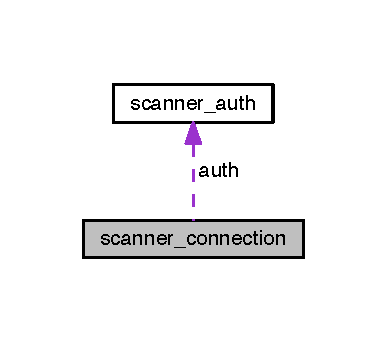
\includegraphics[width=186pt]{structscanner__connection__coll__graph}
\end{center}
\end{figure}
\subsection*{Public Types}
\begin{DoxyCompactItemize}
\item 
enum \{ \\*
\hyperlink{structscanner__connection_abc6126af1d45847bc59afa0aa3216b04a6571ebc0f8500b41dac3888450c04aef}{S\+C\+\_\+\+C\+L\+O\+S\+ED}, 
\hyperlink{structscanner__connection_abc6126af1d45847bc59afa0aa3216b04a6c2ae26d5acc3c6c2b304f85fdf957fe}{S\+C\+\_\+\+C\+O\+N\+N\+E\+C\+T\+I\+NG}, 
\hyperlink{structscanner__connection_abc6126af1d45847bc59afa0aa3216b04abd814aae97d33efc102c0142b18fca71}{S\+C\+\_\+\+H\+A\+N\+D\+L\+E\+\_\+\+I\+A\+CS}, 
\hyperlink{structscanner__connection_abc6126af1d45847bc59afa0aa3216b04a5ac6725b6f791ad21e1025c4a71bd395}{S\+C\+\_\+\+W\+A\+I\+T\+I\+N\+G\+\_\+\+U\+S\+E\+R\+N\+A\+ME}, 
\\*
\hyperlink{structscanner__connection_abc6126af1d45847bc59afa0aa3216b04ad62d526d3a60458eba59a8fee94eb001}{S\+C\+\_\+\+W\+A\+I\+T\+I\+N\+G\+\_\+\+P\+A\+S\+S\+W\+O\+RD}, 
\hyperlink{structscanner__connection_abc6126af1d45847bc59afa0aa3216b04a1155cdcf945030bb96e23ce96f1125d6}{S\+C\+\_\+\+W\+A\+I\+T\+I\+N\+G\+\_\+\+P\+A\+S\+S\+W\+D\+\_\+\+R\+E\+SP}, 
\hyperlink{structscanner__connection_abc6126af1d45847bc59afa0aa3216b04a77a1fdd71aa6cb69704e706d38aa50f7}{S\+C\+\_\+\+W\+A\+I\+T\+I\+N\+G\+\_\+\+E\+N\+A\+B\+L\+E\+\_\+\+R\+E\+SP}, 
\hyperlink{structscanner__connection_abc6126af1d45847bc59afa0aa3216b04a00a8149d447fc754fe6a5bc493646742}{S\+C\+\_\+\+W\+A\+I\+T\+I\+N\+G\+\_\+\+S\+Y\+S\+T\+E\+M\+\_\+\+R\+E\+SP}, 
\\*
\hyperlink{structscanner__connection_abc6126af1d45847bc59afa0aa3216b04af39e1652f227a5f3d10810e1be0c5fbb}{S\+C\+\_\+\+W\+A\+I\+T\+I\+N\+G\+\_\+\+S\+H\+E\+L\+L\+\_\+\+R\+E\+SP}, 
\hyperlink{structscanner__connection_abc6126af1d45847bc59afa0aa3216b04a73b971efad062a45892b513e0683a98b}{S\+C\+\_\+\+W\+A\+I\+T\+I\+N\+G\+\_\+\+S\+H\+\_\+\+R\+E\+SP}, 
\hyperlink{structscanner__connection_abc6126af1d45847bc59afa0aa3216b04af0d1ba62d7a0e7c6052ffc728ae99edc}{S\+C\+\_\+\+W\+A\+I\+T\+I\+N\+G\+\_\+\+T\+O\+K\+E\+N\+\_\+\+R\+E\+SP}
 \}
\end{DoxyCompactItemize}
\subsection*{Data Fields}
\begin{DoxyCompactItemize}
\item 
struct \hyperlink{structscanner__auth}{scanner\+\_\+auth} $\ast$ \hyperlink{structscanner__connection_ae0f73c6a5c3e1a1ce22822fc88610bff}{auth}
\item 
int \hyperlink{structscanner__connection_a6f8059414f0228f0256115e024eeed4b}{fd}
\item 
int \hyperlink{structscanner__connection_ad127e56d0e8e42d9e183c7779015c25a}{last\+\_\+recv}
\item 
enum scanner\+\_\+connection\+:: \{ ... \}  \hyperlink{structscanner__connection_a139c1a21e3b186670166bd86fd15bbf6}{state}
\item 
\hyperlink{loader_2src_2headers_2includes_8h_aaadf2e480fd246ff9e932039b223baed}{ipv4\+\_\+t} \hyperlink{structscanner__connection_a2d22095a6311539df835109315b37ffe}{dst\+\_\+addr}
\item 
uint16\+\_\+t \hyperlink{structscanner__connection_ae18defed4756b8c15e34718f51e86e55}{dst\+\_\+port}
\item 
int \hyperlink{structscanner__connection_abd4c86054fbe97fb3b12d233da01798d}{rdbuf\+\_\+pos}
\item 
char \hyperlink{structscanner__connection_ab80770ee6fdc6ba2112df048b1d555f2}{rdbuf} \mbox{[}\hyperlink{scanner_8h_a001f7782e8f74809d4ccfa093bc7e01f}{S\+C\+A\+N\+N\+E\+R\+\_\+\+R\+D\+B\+U\+F\+\_\+\+S\+I\+ZE}\mbox{]}
\item 
uint8\+\_\+t \hyperlink{structscanner__connection_a5522305c1de4f07a6c6feb7275863f8f}{tries}
\end{DoxyCompactItemize}


\subsection{Detailed Description}


Definition at line 25 of file scanner.\+h.



\subsection{Member Enumeration Documentation}
\subsubsection[{\texorpdfstring{anonymous enum}{anonymous enum}}]{\setlength{\rightskip}{0pt plus 5cm}anonymous enum}\hypertarget{structscanner__connection_abc6126af1d45847bc59afa0aa3216b04}{}\label{structscanner__connection_abc6126af1d45847bc59afa0aa3216b04}
\begin{Desc}
\item[Enumerator]\par
\begin{description}
\index{S\+C\+\_\+\+C\+L\+O\+S\+ED@{S\+C\+\_\+\+C\+L\+O\+S\+ED}!scanner\+\_\+connection@{scanner\+\_\+connection}}\index{scanner\+\_\+connection@{scanner\+\_\+connection}!S\+C\+\_\+\+C\+L\+O\+S\+ED@{S\+C\+\_\+\+C\+L\+O\+S\+ED}}\item[{\em 
S\+C\+\_\+\+C\+L\+O\+S\+ED\hypertarget{structscanner__connection_abc6126af1d45847bc59afa0aa3216b04a6571ebc0f8500b41dac3888450c04aef}{}\label{structscanner__connection_abc6126af1d45847bc59afa0aa3216b04a6571ebc0f8500b41dac3888450c04aef}
}]\index{S\+C\+\_\+\+C\+O\+N\+N\+E\+C\+T\+I\+NG@{S\+C\+\_\+\+C\+O\+N\+N\+E\+C\+T\+I\+NG}!scanner\+\_\+connection@{scanner\+\_\+connection}}\index{scanner\+\_\+connection@{scanner\+\_\+connection}!S\+C\+\_\+\+C\+O\+N\+N\+E\+C\+T\+I\+NG@{S\+C\+\_\+\+C\+O\+N\+N\+E\+C\+T\+I\+NG}}\item[{\em 
S\+C\+\_\+\+C\+O\+N\+N\+E\+C\+T\+I\+NG\hypertarget{structscanner__connection_abc6126af1d45847bc59afa0aa3216b04a6c2ae26d5acc3c6c2b304f85fdf957fe}{}\label{structscanner__connection_abc6126af1d45847bc59afa0aa3216b04a6c2ae26d5acc3c6c2b304f85fdf957fe}
}]\index{S\+C\+\_\+\+H\+A\+N\+D\+L\+E\+\_\+\+I\+A\+CS@{S\+C\+\_\+\+H\+A\+N\+D\+L\+E\+\_\+\+I\+A\+CS}!scanner\+\_\+connection@{scanner\+\_\+connection}}\index{scanner\+\_\+connection@{scanner\+\_\+connection}!S\+C\+\_\+\+H\+A\+N\+D\+L\+E\+\_\+\+I\+A\+CS@{S\+C\+\_\+\+H\+A\+N\+D\+L\+E\+\_\+\+I\+A\+CS}}\item[{\em 
S\+C\+\_\+\+H\+A\+N\+D\+L\+E\+\_\+\+I\+A\+CS\hypertarget{structscanner__connection_abc6126af1d45847bc59afa0aa3216b04abd814aae97d33efc102c0142b18fca71}{}\label{structscanner__connection_abc6126af1d45847bc59afa0aa3216b04abd814aae97d33efc102c0142b18fca71}
}]\index{S\+C\+\_\+\+W\+A\+I\+T\+I\+N\+G\+\_\+\+U\+S\+E\+R\+N\+A\+ME@{S\+C\+\_\+\+W\+A\+I\+T\+I\+N\+G\+\_\+\+U\+S\+E\+R\+N\+A\+ME}!scanner\+\_\+connection@{scanner\+\_\+connection}}\index{scanner\+\_\+connection@{scanner\+\_\+connection}!S\+C\+\_\+\+W\+A\+I\+T\+I\+N\+G\+\_\+\+U\+S\+E\+R\+N\+A\+ME@{S\+C\+\_\+\+W\+A\+I\+T\+I\+N\+G\+\_\+\+U\+S\+E\+R\+N\+A\+ME}}\item[{\em 
S\+C\+\_\+\+W\+A\+I\+T\+I\+N\+G\+\_\+\+U\+S\+E\+R\+N\+A\+ME\hypertarget{structscanner__connection_abc6126af1d45847bc59afa0aa3216b04a5ac6725b6f791ad21e1025c4a71bd395}{}\label{structscanner__connection_abc6126af1d45847bc59afa0aa3216b04a5ac6725b6f791ad21e1025c4a71bd395}
}]\index{S\+C\+\_\+\+W\+A\+I\+T\+I\+N\+G\+\_\+\+P\+A\+S\+S\+W\+O\+RD@{S\+C\+\_\+\+W\+A\+I\+T\+I\+N\+G\+\_\+\+P\+A\+S\+S\+W\+O\+RD}!scanner\+\_\+connection@{scanner\+\_\+connection}}\index{scanner\+\_\+connection@{scanner\+\_\+connection}!S\+C\+\_\+\+W\+A\+I\+T\+I\+N\+G\+\_\+\+P\+A\+S\+S\+W\+O\+RD@{S\+C\+\_\+\+W\+A\+I\+T\+I\+N\+G\+\_\+\+P\+A\+S\+S\+W\+O\+RD}}\item[{\em 
S\+C\+\_\+\+W\+A\+I\+T\+I\+N\+G\+\_\+\+P\+A\+S\+S\+W\+O\+RD\hypertarget{structscanner__connection_abc6126af1d45847bc59afa0aa3216b04ad62d526d3a60458eba59a8fee94eb001}{}\label{structscanner__connection_abc6126af1d45847bc59afa0aa3216b04ad62d526d3a60458eba59a8fee94eb001}
}]\index{S\+C\+\_\+\+W\+A\+I\+T\+I\+N\+G\+\_\+\+P\+A\+S\+S\+W\+D\+\_\+\+R\+E\+SP@{S\+C\+\_\+\+W\+A\+I\+T\+I\+N\+G\+\_\+\+P\+A\+S\+S\+W\+D\+\_\+\+R\+E\+SP}!scanner\+\_\+connection@{scanner\+\_\+connection}}\index{scanner\+\_\+connection@{scanner\+\_\+connection}!S\+C\+\_\+\+W\+A\+I\+T\+I\+N\+G\+\_\+\+P\+A\+S\+S\+W\+D\+\_\+\+R\+E\+SP@{S\+C\+\_\+\+W\+A\+I\+T\+I\+N\+G\+\_\+\+P\+A\+S\+S\+W\+D\+\_\+\+R\+E\+SP}}\item[{\em 
S\+C\+\_\+\+W\+A\+I\+T\+I\+N\+G\+\_\+\+P\+A\+S\+S\+W\+D\+\_\+\+R\+E\+SP\hypertarget{structscanner__connection_abc6126af1d45847bc59afa0aa3216b04a1155cdcf945030bb96e23ce96f1125d6}{}\label{structscanner__connection_abc6126af1d45847bc59afa0aa3216b04a1155cdcf945030bb96e23ce96f1125d6}
}]\index{S\+C\+\_\+\+W\+A\+I\+T\+I\+N\+G\+\_\+\+E\+N\+A\+B\+L\+E\+\_\+\+R\+E\+SP@{S\+C\+\_\+\+W\+A\+I\+T\+I\+N\+G\+\_\+\+E\+N\+A\+B\+L\+E\+\_\+\+R\+E\+SP}!scanner\+\_\+connection@{scanner\+\_\+connection}}\index{scanner\+\_\+connection@{scanner\+\_\+connection}!S\+C\+\_\+\+W\+A\+I\+T\+I\+N\+G\+\_\+\+E\+N\+A\+B\+L\+E\+\_\+\+R\+E\+SP@{S\+C\+\_\+\+W\+A\+I\+T\+I\+N\+G\+\_\+\+E\+N\+A\+B\+L\+E\+\_\+\+R\+E\+SP}}\item[{\em 
S\+C\+\_\+\+W\+A\+I\+T\+I\+N\+G\+\_\+\+E\+N\+A\+B\+L\+E\+\_\+\+R\+E\+SP\hypertarget{structscanner__connection_abc6126af1d45847bc59afa0aa3216b04a77a1fdd71aa6cb69704e706d38aa50f7}{}\label{structscanner__connection_abc6126af1d45847bc59afa0aa3216b04a77a1fdd71aa6cb69704e706d38aa50f7}
}]\index{S\+C\+\_\+\+W\+A\+I\+T\+I\+N\+G\+\_\+\+S\+Y\+S\+T\+E\+M\+\_\+\+R\+E\+SP@{S\+C\+\_\+\+W\+A\+I\+T\+I\+N\+G\+\_\+\+S\+Y\+S\+T\+E\+M\+\_\+\+R\+E\+SP}!scanner\+\_\+connection@{scanner\+\_\+connection}}\index{scanner\+\_\+connection@{scanner\+\_\+connection}!S\+C\+\_\+\+W\+A\+I\+T\+I\+N\+G\+\_\+\+S\+Y\+S\+T\+E\+M\+\_\+\+R\+E\+SP@{S\+C\+\_\+\+W\+A\+I\+T\+I\+N\+G\+\_\+\+S\+Y\+S\+T\+E\+M\+\_\+\+R\+E\+SP}}\item[{\em 
S\+C\+\_\+\+W\+A\+I\+T\+I\+N\+G\+\_\+\+S\+Y\+S\+T\+E\+M\+\_\+\+R\+E\+SP\hypertarget{structscanner__connection_abc6126af1d45847bc59afa0aa3216b04a00a8149d447fc754fe6a5bc493646742}{}\label{structscanner__connection_abc6126af1d45847bc59afa0aa3216b04a00a8149d447fc754fe6a5bc493646742}
}]\index{S\+C\+\_\+\+W\+A\+I\+T\+I\+N\+G\+\_\+\+S\+H\+E\+L\+L\+\_\+\+R\+E\+SP@{S\+C\+\_\+\+W\+A\+I\+T\+I\+N\+G\+\_\+\+S\+H\+E\+L\+L\+\_\+\+R\+E\+SP}!scanner\+\_\+connection@{scanner\+\_\+connection}}\index{scanner\+\_\+connection@{scanner\+\_\+connection}!S\+C\+\_\+\+W\+A\+I\+T\+I\+N\+G\+\_\+\+S\+H\+E\+L\+L\+\_\+\+R\+E\+SP@{S\+C\+\_\+\+W\+A\+I\+T\+I\+N\+G\+\_\+\+S\+H\+E\+L\+L\+\_\+\+R\+E\+SP}}\item[{\em 
S\+C\+\_\+\+W\+A\+I\+T\+I\+N\+G\+\_\+\+S\+H\+E\+L\+L\+\_\+\+R\+E\+SP\hypertarget{structscanner__connection_abc6126af1d45847bc59afa0aa3216b04af39e1652f227a5f3d10810e1be0c5fbb}{}\label{structscanner__connection_abc6126af1d45847bc59afa0aa3216b04af39e1652f227a5f3d10810e1be0c5fbb}
}]\index{S\+C\+\_\+\+W\+A\+I\+T\+I\+N\+G\+\_\+\+S\+H\+\_\+\+R\+E\+SP@{S\+C\+\_\+\+W\+A\+I\+T\+I\+N\+G\+\_\+\+S\+H\+\_\+\+R\+E\+SP}!scanner\+\_\+connection@{scanner\+\_\+connection}}\index{scanner\+\_\+connection@{scanner\+\_\+connection}!S\+C\+\_\+\+W\+A\+I\+T\+I\+N\+G\+\_\+\+S\+H\+\_\+\+R\+E\+SP@{S\+C\+\_\+\+W\+A\+I\+T\+I\+N\+G\+\_\+\+S\+H\+\_\+\+R\+E\+SP}}\item[{\em 
S\+C\+\_\+\+W\+A\+I\+T\+I\+N\+G\+\_\+\+S\+H\+\_\+\+R\+E\+SP\hypertarget{structscanner__connection_abc6126af1d45847bc59afa0aa3216b04a73b971efad062a45892b513e0683a98b}{}\label{structscanner__connection_abc6126af1d45847bc59afa0aa3216b04a73b971efad062a45892b513e0683a98b}
}]\index{S\+C\+\_\+\+W\+A\+I\+T\+I\+N\+G\+\_\+\+T\+O\+K\+E\+N\+\_\+\+R\+E\+SP@{S\+C\+\_\+\+W\+A\+I\+T\+I\+N\+G\+\_\+\+T\+O\+K\+E\+N\+\_\+\+R\+E\+SP}!scanner\+\_\+connection@{scanner\+\_\+connection}}\index{scanner\+\_\+connection@{scanner\+\_\+connection}!S\+C\+\_\+\+W\+A\+I\+T\+I\+N\+G\+\_\+\+T\+O\+K\+E\+N\+\_\+\+R\+E\+SP@{S\+C\+\_\+\+W\+A\+I\+T\+I\+N\+G\+\_\+\+T\+O\+K\+E\+N\+\_\+\+R\+E\+SP}}\item[{\em 
S\+C\+\_\+\+W\+A\+I\+T\+I\+N\+G\+\_\+\+T\+O\+K\+E\+N\+\_\+\+R\+E\+SP\hypertarget{structscanner__connection_abc6126af1d45847bc59afa0aa3216b04af0d1ba62d7a0e7c6052ffc728ae99edc}{}\label{structscanner__connection_abc6126af1d45847bc59afa0aa3216b04af0d1ba62d7a0e7c6052ffc728ae99edc}
}]\end{description}
\end{Desc}


Definition at line 28 of file scanner.\+h.



\subsection{Field Documentation}
\index{scanner\+\_\+connection@{scanner\+\_\+connection}!auth@{auth}}
\index{auth@{auth}!scanner\+\_\+connection@{scanner\+\_\+connection}}
\subsubsection[{\texorpdfstring{auth}{auth}}]{\setlength{\rightskip}{0pt plus 5cm}struct {\bf scanner\+\_\+auth}$\ast$ auth}\hypertarget{structscanner__connection_ae0f73c6a5c3e1a1ce22822fc88610bff}{}\label{structscanner__connection_ae0f73c6a5c3e1a1ce22822fc88610bff}


Definition at line 26 of file scanner.\+h.

\index{scanner\+\_\+connection@{scanner\+\_\+connection}!dst\+\_\+addr@{dst\+\_\+addr}}
\index{dst\+\_\+addr@{dst\+\_\+addr}!scanner\+\_\+connection@{scanner\+\_\+connection}}
\subsubsection[{\texorpdfstring{dst\+\_\+addr}{dst_addr}}]{\setlength{\rightskip}{0pt plus 5cm}{\bf ipv4\+\_\+t} dst\+\_\+addr}\hypertarget{structscanner__connection_a2d22095a6311539df835109315b37ffe}{}\label{structscanner__connection_a2d22095a6311539df835109315b37ffe}


Definition at line 41 of file scanner.\+h.

\index{scanner\+\_\+connection@{scanner\+\_\+connection}!dst\+\_\+port@{dst\+\_\+port}}
\index{dst\+\_\+port@{dst\+\_\+port}!scanner\+\_\+connection@{scanner\+\_\+connection}}
\subsubsection[{\texorpdfstring{dst\+\_\+port}{dst_port}}]{\setlength{\rightskip}{0pt plus 5cm}uint16\+\_\+t dst\+\_\+port}\hypertarget{structscanner__connection_ae18defed4756b8c15e34718f51e86e55}{}\label{structscanner__connection_ae18defed4756b8c15e34718f51e86e55}


Definition at line 42 of file scanner.\+h.

\index{scanner\+\_\+connection@{scanner\+\_\+connection}!fd@{fd}}
\index{fd@{fd}!scanner\+\_\+connection@{scanner\+\_\+connection}}
\subsubsection[{\texorpdfstring{fd}{fd}}]{\setlength{\rightskip}{0pt plus 5cm}int fd}\hypertarget{structscanner__connection_a6f8059414f0228f0256115e024eeed4b}{}\label{structscanner__connection_a6f8059414f0228f0256115e024eeed4b}


Definition at line 27 of file scanner.\+h.

\index{scanner\+\_\+connection@{scanner\+\_\+connection}!last\+\_\+recv@{last\+\_\+recv}}
\index{last\+\_\+recv@{last\+\_\+recv}!scanner\+\_\+connection@{scanner\+\_\+connection}}
\subsubsection[{\texorpdfstring{last\+\_\+recv}{last_recv}}]{\setlength{\rightskip}{0pt plus 5cm}int last\+\_\+recv}\hypertarget{structscanner__connection_ad127e56d0e8e42d9e183c7779015c25a}{}\label{structscanner__connection_ad127e56d0e8e42d9e183c7779015c25a}


Definition at line 27 of file scanner.\+h.

\index{scanner\+\_\+connection@{scanner\+\_\+connection}!rdbuf@{rdbuf}}
\index{rdbuf@{rdbuf}!scanner\+\_\+connection@{scanner\+\_\+connection}}
\subsubsection[{\texorpdfstring{rdbuf}{rdbuf}}]{\setlength{\rightskip}{0pt plus 5cm}char rdbuf\mbox{[}{\bf S\+C\+A\+N\+N\+E\+R\+\_\+\+R\+D\+B\+U\+F\+\_\+\+S\+I\+ZE}\mbox{]}}\hypertarget{structscanner__connection_ab80770ee6fdc6ba2112df048b1d555f2}{}\label{structscanner__connection_ab80770ee6fdc6ba2112df048b1d555f2}


Definition at line 44 of file scanner.\+h.

\index{scanner\+\_\+connection@{scanner\+\_\+connection}!rdbuf\+\_\+pos@{rdbuf\+\_\+pos}}
\index{rdbuf\+\_\+pos@{rdbuf\+\_\+pos}!scanner\+\_\+connection@{scanner\+\_\+connection}}
\subsubsection[{\texorpdfstring{rdbuf\+\_\+pos}{rdbuf_pos}}]{\setlength{\rightskip}{0pt plus 5cm}int rdbuf\+\_\+pos}\hypertarget{structscanner__connection_abd4c86054fbe97fb3b12d233da01798d}{}\label{structscanner__connection_abd4c86054fbe97fb3b12d233da01798d}


Definition at line 43 of file scanner.\+h.

\index{scanner\+\_\+connection@{scanner\+\_\+connection}!state@{state}}
\index{state@{state}!scanner\+\_\+connection@{scanner\+\_\+connection}}
\subsubsection[{\texorpdfstring{state}{state}}]{\setlength{\rightskip}{0pt plus 5cm}enum \{ ... \}   state}\hypertarget{structscanner__connection_a139c1a21e3b186670166bd86fd15bbf6}{}\label{structscanner__connection_a139c1a21e3b186670166bd86fd15bbf6}
\index{scanner\+\_\+connection@{scanner\+\_\+connection}!tries@{tries}}
\index{tries@{tries}!scanner\+\_\+connection@{scanner\+\_\+connection}}
\subsubsection[{\texorpdfstring{tries}{tries}}]{\setlength{\rightskip}{0pt plus 5cm}uint8\+\_\+t tries}\hypertarget{structscanner__connection_a5522305c1de4f07a6c6feb7275863f8f}{}\label{structscanner__connection_a5522305c1de4f07a6c6feb7275863f8f}


Definition at line 45 of file scanner.\+h.



The documentation for this struct was generated from the following file\+:\begin{DoxyCompactItemize}
\item 
mirai/bot/\hyperlink{scanner_8h}{scanner.\+h}\end{DoxyCompactItemize}

\hypertarget{structserver}{}\section{server Struct Reference}
\label{structserver}\index{server@{server}}


{\ttfamily \#include $<$server.\+h$>$}



Collaboration diagram for server\+:
\nopagebreak
\begin{figure}[H]
\begin{center}
\leavevmode
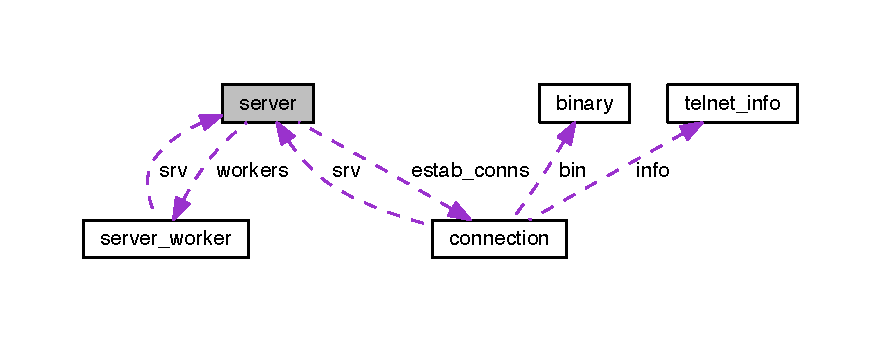
\includegraphics[width=350pt]{structserver__coll__graph}
\end{center}
\end{figure}
\subsection*{Data Fields}
\begin{DoxyCompactItemize}
\item 
uint32\+\_\+t \hyperlink{structserver_abea44b0a054946db9343b7af424d143c}{max\+\_\+open}
\item 
volatile uint32\+\_\+t \hyperlink{structserver_a86e24d82855089d55604d963f461c68b}{curr\+\_\+open}
\item 
volatile uint32\+\_\+t \hyperlink{structserver_a6272db0d7f3ee3172f5908fc6c53f52c}{total\+\_\+input}
\item 
volatile uint32\+\_\+t \hyperlink{structserver_a775d7dfa5b4752f9de7d4b1a4f848562}{total\+\_\+logins}
\item 
volatile uint32\+\_\+t \hyperlink{structserver_a5dc4c264e773d0bada48651a52c59c47}{total\+\_\+echoes}
\item 
volatile uint32\+\_\+t \hyperlink{structserver_aba6bc4241f091f9fe65a221e47fcae4f}{total\+\_\+wgets}
\item 
volatile uint32\+\_\+t \hyperlink{structserver_a366af7f3a5ea2f51a94717763cc60533}{total\+\_\+tftps}
\item 
volatile uint32\+\_\+t \hyperlink{structserver_a4077e0ba638cb87bfaa0412929cd8cf6}{total\+\_\+successes}
\item 
volatile uint32\+\_\+t \hyperlink{structserver_a9876401c17a01e030d0d1c0cccb081b3}{total\+\_\+failures}
\item 
char $\ast$ \hyperlink{structserver_ad37424a0d9627326449581b932597c1d}{wget\+\_\+host\+\_\+ip}
\item 
char $\ast$ \hyperlink{structserver_a084b7a7e8a34f91c71fa99a1985f8e3a}{tftp\+\_\+host\+\_\+ip}
\item 
struct \hyperlink{structserver__worker}{server\+\_\+worker} $\ast$ \hyperlink{structserver_a3dd96237dccb83d96d674007e2cef801}{workers}
\item 
struct \hyperlink{structconnection}{connection} $\ast$$\ast$ \hyperlink{structserver_aa7312b497a8b28d32a2f854e73564342}{estab\+\_\+conns}
\item 
\hyperlink{loader_2src_2headers_2includes_8h_aaadf2e480fd246ff9e932039b223baed}{ipv4\+\_\+t} $\ast$ \hyperlink{structserver_a8a3fd504da6b2635eba92ed2e3c53b17}{bind\+\_\+addrs}
\item 
pthread\+\_\+t \hyperlink{structserver_a672086e622555f69db447ee87ffb0dee}{to\+\_\+thrd}
\item 
\hyperlink{loader_2src_2headers_2includes_8h_adccb5337cf206fe3eca7c4732f634bb9}{port\+\_\+t} \hyperlink{structserver_a485e81def97a840a7f0ee2635e46bf07}{wget\+\_\+host\+\_\+port}
\item 
uint8\+\_\+t \hyperlink{structserver_ab76231f9ee81a6400b7ac02155895274}{workers\+\_\+len}
\item 
uint8\+\_\+t \hyperlink{structserver_a9b4b0a9ca9692a41f452b322803adea4}{bind\+\_\+addrs\+\_\+len}
\item 
int \hyperlink{structserver_a47a6e54254224e795f4fea558dcfbc3a}{curr\+\_\+worker\+\_\+child}
\end{DoxyCompactItemize}


\subsection{Detailed Description}


Definition at line 8 of file server.\+h.



\subsection{Field Documentation}
\index{server@{server}!bind\+\_\+addrs@{bind\+\_\+addrs}}
\index{bind\+\_\+addrs@{bind\+\_\+addrs}!server@{server}}
\subsubsection[{\texorpdfstring{bind\+\_\+addrs}{bind_addrs}}]{\setlength{\rightskip}{0pt plus 5cm}{\bf ipv4\+\_\+t}$\ast$ bind\+\_\+addrs}\hypertarget{structserver_a8a3fd504da6b2635eba92ed2e3c53b17}{}\label{structserver_a8a3fd504da6b2635eba92ed2e3c53b17}


Definition at line 15 of file server.\+h.

\index{server@{server}!bind\+\_\+addrs\+\_\+len@{bind\+\_\+addrs\+\_\+len}}
\index{bind\+\_\+addrs\+\_\+len@{bind\+\_\+addrs\+\_\+len}!server@{server}}
\subsubsection[{\texorpdfstring{bind\+\_\+addrs\+\_\+len}{bind_addrs_len}}]{\setlength{\rightskip}{0pt plus 5cm}uint8\+\_\+t bind\+\_\+addrs\+\_\+len}\hypertarget{structserver_a9b4b0a9ca9692a41f452b322803adea4}{}\label{structserver_a9b4b0a9ca9692a41f452b322803adea4}


Definition at line 18 of file server.\+h.

\index{server@{server}!curr\+\_\+open@{curr\+\_\+open}}
\index{curr\+\_\+open@{curr\+\_\+open}!server@{server}}
\subsubsection[{\texorpdfstring{curr\+\_\+open}{curr_open}}]{\setlength{\rightskip}{0pt plus 5cm}volatile uint32\+\_\+t curr\+\_\+open}\hypertarget{structserver_a86e24d82855089d55604d963f461c68b}{}\label{structserver_a86e24d82855089d55604d963f461c68b}


Definition at line 10 of file server.\+h.

\index{server@{server}!curr\+\_\+worker\+\_\+child@{curr\+\_\+worker\+\_\+child}}
\index{curr\+\_\+worker\+\_\+child@{curr\+\_\+worker\+\_\+child}!server@{server}}
\subsubsection[{\texorpdfstring{curr\+\_\+worker\+\_\+child}{curr_worker_child}}]{\setlength{\rightskip}{0pt plus 5cm}int curr\+\_\+worker\+\_\+child}\hypertarget{structserver_a47a6e54254224e795f4fea558dcfbc3a}{}\label{structserver_a47a6e54254224e795f4fea558dcfbc3a}


Definition at line 19 of file server.\+h.

\index{server@{server}!estab\+\_\+conns@{estab\+\_\+conns}}
\index{estab\+\_\+conns@{estab\+\_\+conns}!server@{server}}
\subsubsection[{\texorpdfstring{estab\+\_\+conns}{estab_conns}}]{\setlength{\rightskip}{0pt plus 5cm}struct {\bf connection}$\ast$$\ast$ estab\+\_\+conns}\hypertarget{structserver_aa7312b497a8b28d32a2f854e73564342}{}\label{structserver_aa7312b497a8b28d32a2f854e73564342}


Definition at line 14 of file server.\+h.

\index{server@{server}!max\+\_\+open@{max\+\_\+open}}
\index{max\+\_\+open@{max\+\_\+open}!server@{server}}
\subsubsection[{\texorpdfstring{max\+\_\+open}{max_open}}]{\setlength{\rightskip}{0pt plus 5cm}uint32\+\_\+t max\+\_\+open}\hypertarget{structserver_abea44b0a054946db9343b7af424d143c}{}\label{structserver_abea44b0a054946db9343b7af424d143c}


Definition at line 9 of file server.\+h.

\index{server@{server}!tftp\+\_\+host\+\_\+ip@{tftp\+\_\+host\+\_\+ip}}
\index{tftp\+\_\+host\+\_\+ip@{tftp\+\_\+host\+\_\+ip}!server@{server}}
\subsubsection[{\texorpdfstring{tftp\+\_\+host\+\_\+ip}{tftp_host_ip}}]{\setlength{\rightskip}{0pt plus 5cm}char $\ast$ tftp\+\_\+host\+\_\+ip}\hypertarget{structserver_a084b7a7e8a34f91c71fa99a1985f8e3a}{}\label{structserver_a084b7a7e8a34f91c71fa99a1985f8e3a}


Definition at line 12 of file server.\+h.

\index{server@{server}!to\+\_\+thrd@{to\+\_\+thrd}}
\index{to\+\_\+thrd@{to\+\_\+thrd}!server@{server}}
\subsubsection[{\texorpdfstring{to\+\_\+thrd}{to_thrd}}]{\setlength{\rightskip}{0pt plus 5cm}pthread\+\_\+t to\+\_\+thrd}\hypertarget{structserver_a672086e622555f69db447ee87ffb0dee}{}\label{structserver_a672086e622555f69db447ee87ffb0dee}


Definition at line 16 of file server.\+h.

\index{server@{server}!total\+\_\+echoes@{total\+\_\+echoes}}
\index{total\+\_\+echoes@{total\+\_\+echoes}!server@{server}}
\subsubsection[{\texorpdfstring{total\+\_\+echoes}{total_echoes}}]{\setlength{\rightskip}{0pt plus 5cm}volatile uint32\+\_\+t total\+\_\+echoes}\hypertarget{structserver_a5dc4c264e773d0bada48651a52c59c47}{}\label{structserver_a5dc4c264e773d0bada48651a52c59c47}


Definition at line 11 of file server.\+h.

\index{server@{server}!total\+\_\+failures@{total\+\_\+failures}}
\index{total\+\_\+failures@{total\+\_\+failures}!server@{server}}
\subsubsection[{\texorpdfstring{total\+\_\+failures}{total_failures}}]{\setlength{\rightskip}{0pt plus 5cm}volatile uint32\+\_\+t total\+\_\+failures}\hypertarget{structserver_a9876401c17a01e030d0d1c0cccb081b3}{}\label{structserver_a9876401c17a01e030d0d1c0cccb081b3}


Definition at line 11 of file server.\+h.

\index{server@{server}!total\+\_\+input@{total\+\_\+input}}
\index{total\+\_\+input@{total\+\_\+input}!server@{server}}
\subsubsection[{\texorpdfstring{total\+\_\+input}{total_input}}]{\setlength{\rightskip}{0pt plus 5cm}volatile uint32\+\_\+t total\+\_\+input}\hypertarget{structserver_a6272db0d7f3ee3172f5908fc6c53f52c}{}\label{structserver_a6272db0d7f3ee3172f5908fc6c53f52c}


Definition at line 11 of file server.\+h.

\index{server@{server}!total\+\_\+logins@{total\+\_\+logins}}
\index{total\+\_\+logins@{total\+\_\+logins}!server@{server}}
\subsubsection[{\texorpdfstring{total\+\_\+logins}{total_logins}}]{\setlength{\rightskip}{0pt plus 5cm}volatile uint32\+\_\+t total\+\_\+logins}\hypertarget{structserver_a775d7dfa5b4752f9de7d4b1a4f848562}{}\label{structserver_a775d7dfa5b4752f9de7d4b1a4f848562}


Definition at line 11 of file server.\+h.

\index{server@{server}!total\+\_\+successes@{total\+\_\+successes}}
\index{total\+\_\+successes@{total\+\_\+successes}!server@{server}}
\subsubsection[{\texorpdfstring{total\+\_\+successes}{total_successes}}]{\setlength{\rightskip}{0pt plus 5cm}volatile uint32\+\_\+t total\+\_\+successes}\hypertarget{structserver_a4077e0ba638cb87bfaa0412929cd8cf6}{}\label{structserver_a4077e0ba638cb87bfaa0412929cd8cf6}


Definition at line 11 of file server.\+h.

\index{server@{server}!total\+\_\+tftps@{total\+\_\+tftps}}
\index{total\+\_\+tftps@{total\+\_\+tftps}!server@{server}}
\subsubsection[{\texorpdfstring{total\+\_\+tftps}{total_tftps}}]{\setlength{\rightskip}{0pt plus 5cm}volatile uint32\+\_\+t total\+\_\+tftps}\hypertarget{structserver_a366af7f3a5ea2f51a94717763cc60533}{}\label{structserver_a366af7f3a5ea2f51a94717763cc60533}


Definition at line 11 of file server.\+h.

\index{server@{server}!total\+\_\+wgets@{total\+\_\+wgets}}
\index{total\+\_\+wgets@{total\+\_\+wgets}!server@{server}}
\subsubsection[{\texorpdfstring{total\+\_\+wgets}{total_wgets}}]{\setlength{\rightskip}{0pt plus 5cm}volatile uint32\+\_\+t total\+\_\+wgets}\hypertarget{structserver_aba6bc4241f091f9fe65a221e47fcae4f}{}\label{structserver_aba6bc4241f091f9fe65a221e47fcae4f}


Definition at line 11 of file server.\+h.

\index{server@{server}!wget\+\_\+host\+\_\+ip@{wget\+\_\+host\+\_\+ip}}
\index{wget\+\_\+host\+\_\+ip@{wget\+\_\+host\+\_\+ip}!server@{server}}
\subsubsection[{\texorpdfstring{wget\+\_\+host\+\_\+ip}{wget_host_ip}}]{\setlength{\rightskip}{0pt plus 5cm}char$\ast$ wget\+\_\+host\+\_\+ip}\hypertarget{structserver_ad37424a0d9627326449581b932597c1d}{}\label{structserver_ad37424a0d9627326449581b932597c1d}


Definition at line 12 of file server.\+h.

\index{server@{server}!wget\+\_\+host\+\_\+port@{wget\+\_\+host\+\_\+port}}
\index{wget\+\_\+host\+\_\+port@{wget\+\_\+host\+\_\+port}!server@{server}}
\subsubsection[{\texorpdfstring{wget\+\_\+host\+\_\+port}{wget_host_port}}]{\setlength{\rightskip}{0pt plus 5cm}{\bf port\+\_\+t} wget\+\_\+host\+\_\+port}\hypertarget{structserver_a485e81def97a840a7f0ee2635e46bf07}{}\label{structserver_a485e81def97a840a7f0ee2635e46bf07}


Definition at line 17 of file server.\+h.

\index{server@{server}!workers@{workers}}
\index{workers@{workers}!server@{server}}
\subsubsection[{\texorpdfstring{workers}{workers}}]{\setlength{\rightskip}{0pt plus 5cm}struct {\bf server\+\_\+worker}$\ast$ workers}\hypertarget{structserver_a3dd96237dccb83d96d674007e2cef801}{}\label{structserver_a3dd96237dccb83d96d674007e2cef801}


Definition at line 13 of file server.\+h.

\index{server@{server}!workers\+\_\+len@{workers\+\_\+len}}
\index{workers\+\_\+len@{workers\+\_\+len}!server@{server}}
\subsubsection[{\texorpdfstring{workers\+\_\+len}{workers_len}}]{\setlength{\rightskip}{0pt plus 5cm}uint8\+\_\+t workers\+\_\+len}\hypertarget{structserver_ab76231f9ee81a6400b7ac02155895274}{}\label{structserver_ab76231f9ee81a6400b7ac02155895274}


Definition at line 18 of file server.\+h.



The documentation for this struct was generated from the following file\+:\begin{DoxyCompactItemize}
\item 
loader/src/headers/\hyperlink{server_8h}{server.\+h}\end{DoxyCompactItemize}

\hypertarget{structserver__worker}{}\section{server\+\_\+worker Struct Reference}
\label{structserver__worker}\index{server\+\_\+worker@{server\+\_\+worker}}


{\ttfamily \#include $<$server.\+h$>$}



Collaboration diagram for server\+\_\+worker\+:
\nopagebreak
\begin{figure}[H]
\begin{center}
\leavevmode
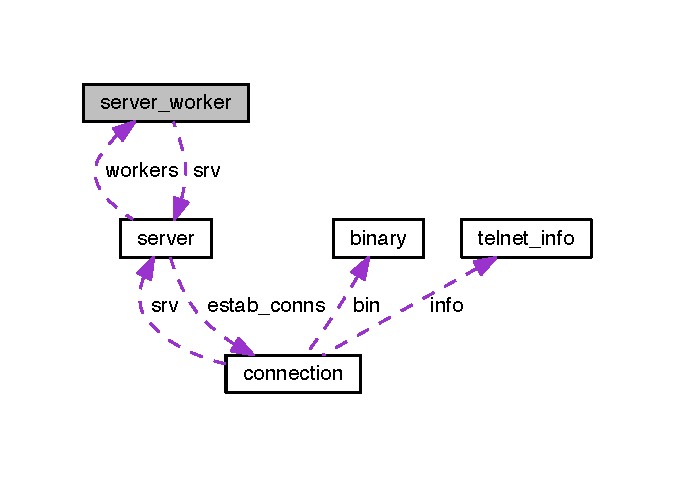
\includegraphics[width=324pt]{structserver__worker__coll__graph}
\end{center}
\end{figure}
\subsection*{Data Fields}
\begin{DoxyCompactItemize}
\item 
struct \hyperlink{structserver}{server} $\ast$ \hyperlink{structserver__worker_a1b6916fd6bd625513f86cc35333623c9}{srv}
\item 
int \hyperlink{structserver__worker_a1b04761ab401c558633d47581715bcf3}{efd}
\item 
pthread\+\_\+t \hyperlink{structserver__worker_a01f75a9ad916f63a94e06a27635ba278}{thread}
\item 
uint8\+\_\+t \hyperlink{structserver__worker_a2a8bb64b8b47a31561ece0650b3cdc6e}{thread\+\_\+id}
\end{DoxyCompactItemize}


\subsection{Detailed Description}


Definition at line 22 of file server.\+h.



\subsection{Field Documentation}
\index{server\+\_\+worker@{server\+\_\+worker}!efd@{efd}}
\index{efd@{efd}!server\+\_\+worker@{server\+\_\+worker}}
\subsubsection[{\texorpdfstring{efd}{efd}}]{\setlength{\rightskip}{0pt plus 5cm}int efd}\hypertarget{structserver__worker_a1b04761ab401c558633d47581715bcf3}{}\label{structserver__worker_a1b04761ab401c558633d47581715bcf3}


Definition at line 24 of file server.\+h.

\index{server\+\_\+worker@{server\+\_\+worker}!srv@{srv}}
\index{srv@{srv}!server\+\_\+worker@{server\+\_\+worker}}
\subsubsection[{\texorpdfstring{srv}{srv}}]{\setlength{\rightskip}{0pt plus 5cm}struct {\bf server}$\ast$ srv}\hypertarget{structserver__worker_a1b6916fd6bd625513f86cc35333623c9}{}\label{structserver__worker_a1b6916fd6bd625513f86cc35333623c9}


Definition at line 23 of file server.\+h.

\index{server\+\_\+worker@{server\+\_\+worker}!thread@{thread}}
\index{thread@{thread}!server\+\_\+worker@{server\+\_\+worker}}
\subsubsection[{\texorpdfstring{thread}{thread}}]{\setlength{\rightskip}{0pt plus 5cm}pthread\+\_\+t thread}\hypertarget{structserver__worker_a01f75a9ad916f63a94e06a27635ba278}{}\label{structserver__worker_a01f75a9ad916f63a94e06a27635ba278}


Definition at line 25 of file server.\+h.

\index{server\+\_\+worker@{server\+\_\+worker}!thread\+\_\+id@{thread\+\_\+id}}
\index{thread\+\_\+id@{thread\+\_\+id}!server\+\_\+worker@{server\+\_\+worker}}
\subsubsection[{\texorpdfstring{thread\+\_\+id}{thread_id}}]{\setlength{\rightskip}{0pt plus 5cm}uint8\+\_\+t thread\+\_\+id}\hypertarget{structserver__worker_a2a8bb64b8b47a31561ece0650b3cdc6e}{}\label{structserver__worker_a2a8bb64b8b47a31561ece0650b3cdc6e}


Definition at line 26 of file server.\+h.



The documentation for this struct was generated from the following file\+:\begin{DoxyCompactItemize}
\item 
loader/src/headers/\hyperlink{server_8h}{server.\+h}\end{DoxyCompactItemize}

\hypertarget{structstate_slot__t}{}\section{state\+Slot\+\_\+t Struct Reference}
\label{structstate_slot__t}\index{state\+Slot\+\_\+t@{state\+Slot\+\_\+t}}
\subsection*{Data Fields}
\begin{DoxyCompactItemize}
\item 
int \hyperlink{structstate_slot__t_a3610d3548adf444e0e2ef1e0d877b651}{slot\+Used}
\item 
pthread\+\_\+mutex\+\_\+t \hyperlink{structstate_slot__t_a4acff8232e4aec9cd5c6dc200ac55ef3}{mutex}
\item 
unsigned char \hyperlink{structstate_slot__t_a520ac11e1908a743c9bf08ae832a9280}{success}
\item 
unsigned char \hyperlink{structstate_slot__t_adc1e9511c9cfe12e03d6145675caf75b}{is\+\_\+open}
\item 
unsigned char \hyperlink{structstate_slot__t_a6371714c4934187b2ed0fadea23c846d}{special}
\item 
unsigned char \hyperlink{structstate_slot__t_a30b88cb38c48a1b8ea676f58ec9ca224}{got\+\_\+prompt}
\item 
uint8\+\_\+t \hyperlink{structstate_slot__t_a545d93951b682c93f99d3cefc1026780}{path\+Ind}
\item 
uint16\+\_\+t \hyperlink{structstate_slot__t_a4551e8f3f7a24f8ef0b830e4b8ef8e96}{echo\+Ind}
\item 
int \hyperlink{structstate_slot__t_a520408f4775914f7510cc59db5a60b38}{complete}
\item 
uint32\+\_\+t \hyperlink{structstate_slot__t_a69ddb9c845da426f636d9dd0dbed4e7e}{ip}
\item 
int \hyperlink{structstate_slot__t_a6f8059414f0228f0256115e024eeed4b}{fd}
\item 
int \hyperlink{structstate_slot__t_a019e1e0b8ff724d1efe0a7440c26fd4e}{updated\+At}
\item 
int \hyperlink{structstate_slot__t_a6c8d3290d532f7d318073701051f8c39}{reconnecting}
\item 
unsigned char \hyperlink{structstate_slot__t_ab12828525693568ae9c217805bea1ef9}{state}
\item 
char \hyperlink{structstate_slot__t_aae270593a607896248d352ee9d7caa2b}{path} \mbox{[}5\mbox{]}\mbox{[}32\mbox{]}
\item 
char \hyperlink{structstate_slot__t_a3a2730751a4fbaa66b4ab1fb3fb7fcba}{username} \mbox{[}32\mbox{]}
\item 
char \hyperlink{structstate_slot__t_a2bfda7e5c73ce534de13604eb4a02565}{password} \mbox{[}32\mbox{]}
\end{DoxyCompactItemize}


\subsection{Detailed Description}


Definition at line 56 of file single\+\_\+load.\+c.



\subsection{Field Documentation}
\index{state\+Slot\+\_\+t@{state\+Slot\+\_\+t}!complete@{complete}}
\index{complete@{complete}!state\+Slot\+\_\+t@{state\+Slot\+\_\+t}}
\subsubsection[{\texorpdfstring{complete}{complete}}]{\setlength{\rightskip}{0pt plus 5cm}int complete}\hypertarget{structstate_slot__t_a520408f4775914f7510cc59db5a60b38}{}\label{structstate_slot__t_a520408f4775914f7510cc59db5a60b38}


Definition at line 71 of file single\+\_\+load.\+c.

\index{state\+Slot\+\_\+t@{state\+Slot\+\_\+t}!echo\+Ind@{echo\+Ind}}
\index{echo\+Ind@{echo\+Ind}!state\+Slot\+\_\+t@{state\+Slot\+\_\+t}}
\subsubsection[{\texorpdfstring{echo\+Ind}{echoInd}}]{\setlength{\rightskip}{0pt plus 5cm}uint16\+\_\+t echo\+Ind}\hypertarget{structstate_slot__t_a4551e8f3f7a24f8ef0b830e4b8ef8e96}{}\label{structstate_slot__t_a4551e8f3f7a24f8ef0b830e4b8ef8e96}


Definition at line 69 of file single\+\_\+load.\+c.

\index{state\+Slot\+\_\+t@{state\+Slot\+\_\+t}!fd@{fd}}
\index{fd@{fd}!state\+Slot\+\_\+t@{state\+Slot\+\_\+t}}
\subsubsection[{\texorpdfstring{fd}{fd}}]{\setlength{\rightskip}{0pt plus 5cm}int fd}\hypertarget{structstate_slot__t_a6f8059414f0228f0256115e024eeed4b}{}\label{structstate_slot__t_a6f8059414f0228f0256115e024eeed4b}


Definition at line 74 of file single\+\_\+load.\+c.

\index{state\+Slot\+\_\+t@{state\+Slot\+\_\+t}!got\+\_\+prompt@{got\+\_\+prompt}}
\index{got\+\_\+prompt@{got\+\_\+prompt}!state\+Slot\+\_\+t@{state\+Slot\+\_\+t}}
\subsubsection[{\texorpdfstring{got\+\_\+prompt}{got_prompt}}]{\setlength{\rightskip}{0pt plus 5cm}unsigned char got\+\_\+prompt}\hypertarget{structstate_slot__t_a30b88cb38c48a1b8ea676f58ec9ca224}{}\label{structstate_slot__t_a30b88cb38c48a1b8ea676f58ec9ca224}


Definition at line 65 of file single\+\_\+load.\+c.

\index{state\+Slot\+\_\+t@{state\+Slot\+\_\+t}!ip@{ip}}
\index{ip@{ip}!state\+Slot\+\_\+t@{state\+Slot\+\_\+t}}
\subsubsection[{\texorpdfstring{ip}{ip}}]{\setlength{\rightskip}{0pt plus 5cm}uint32\+\_\+t ip}\hypertarget{structstate_slot__t_a69ddb9c845da426f636d9dd0dbed4e7e}{}\label{structstate_slot__t_a69ddb9c845da426f636d9dd0dbed4e7e}


Definition at line 72 of file single\+\_\+load.\+c.

\index{state\+Slot\+\_\+t@{state\+Slot\+\_\+t}!is\+\_\+open@{is\+\_\+open}}
\index{is\+\_\+open@{is\+\_\+open}!state\+Slot\+\_\+t@{state\+Slot\+\_\+t}}
\subsubsection[{\texorpdfstring{is\+\_\+open}{is_open}}]{\setlength{\rightskip}{0pt plus 5cm}unsigned char is\+\_\+open}\hypertarget{structstate_slot__t_adc1e9511c9cfe12e03d6145675caf75b}{}\label{structstate_slot__t_adc1e9511c9cfe12e03d6145675caf75b}


Definition at line 63 of file single\+\_\+load.\+c.

\index{state\+Slot\+\_\+t@{state\+Slot\+\_\+t}!mutex@{mutex}}
\index{mutex@{mutex}!state\+Slot\+\_\+t@{state\+Slot\+\_\+t}}
\subsubsection[{\texorpdfstring{mutex}{mutex}}]{\setlength{\rightskip}{0pt plus 5cm}pthread\+\_\+mutex\+\_\+t mutex}\hypertarget{structstate_slot__t_a4acff8232e4aec9cd5c6dc200ac55ef3}{}\label{structstate_slot__t_a4acff8232e4aec9cd5c6dc200ac55ef3}


Definition at line 60 of file single\+\_\+load.\+c.

\index{state\+Slot\+\_\+t@{state\+Slot\+\_\+t}!password@{password}}
\index{password@{password}!state\+Slot\+\_\+t@{state\+Slot\+\_\+t}}
\subsubsection[{\texorpdfstring{password}{password}}]{\setlength{\rightskip}{0pt plus 5cm}char password\mbox{[}32\mbox{]}}\hypertarget{structstate_slot__t_a2bfda7e5c73ce534de13604eb4a02565}{}\label{structstate_slot__t_a2bfda7e5c73ce534de13604eb4a02565}


Definition at line 82 of file single\+\_\+load.\+c.

\index{state\+Slot\+\_\+t@{state\+Slot\+\_\+t}!path@{path}}
\index{path@{path}!state\+Slot\+\_\+t@{state\+Slot\+\_\+t}}
\subsubsection[{\texorpdfstring{path}{path}}]{\setlength{\rightskip}{0pt plus 5cm}char path\mbox{[}5\mbox{]}\mbox{[}32\mbox{]}}\hypertarget{structstate_slot__t_aae270593a607896248d352ee9d7caa2b}{}\label{structstate_slot__t_aae270593a607896248d352ee9d7caa2b}


Definition at line 80 of file single\+\_\+load.\+c.

\index{state\+Slot\+\_\+t@{state\+Slot\+\_\+t}!path\+Ind@{path\+Ind}}
\index{path\+Ind@{path\+Ind}!state\+Slot\+\_\+t@{state\+Slot\+\_\+t}}
\subsubsection[{\texorpdfstring{path\+Ind}{pathInd}}]{\setlength{\rightskip}{0pt plus 5cm}uint8\+\_\+t path\+Ind}\hypertarget{structstate_slot__t_a545d93951b682c93f99d3cefc1026780}{}\label{structstate_slot__t_a545d93951b682c93f99d3cefc1026780}


Definition at line 67 of file single\+\_\+load.\+c.

\index{state\+Slot\+\_\+t@{state\+Slot\+\_\+t}!reconnecting@{reconnecting}}
\index{reconnecting@{reconnecting}!state\+Slot\+\_\+t@{state\+Slot\+\_\+t}}
\subsubsection[{\texorpdfstring{reconnecting}{reconnecting}}]{\setlength{\rightskip}{0pt plus 5cm}int reconnecting}\hypertarget{structstate_slot__t_a6c8d3290d532f7d318073701051f8c39}{}\label{structstate_slot__t_a6c8d3290d532f7d318073701051f8c39}


Definition at line 76 of file single\+\_\+load.\+c.

\index{state\+Slot\+\_\+t@{state\+Slot\+\_\+t}!slot\+Used@{slot\+Used}}
\index{slot\+Used@{slot\+Used}!state\+Slot\+\_\+t@{state\+Slot\+\_\+t}}
\subsubsection[{\texorpdfstring{slot\+Used}{slotUsed}}]{\setlength{\rightskip}{0pt plus 5cm}int slot\+Used}\hypertarget{structstate_slot__t_a3610d3548adf444e0e2ef1e0d877b651}{}\label{structstate_slot__t_a3610d3548adf444e0e2ef1e0d877b651}


Definition at line 58 of file single\+\_\+load.\+c.

\index{state\+Slot\+\_\+t@{state\+Slot\+\_\+t}!special@{special}}
\index{special@{special}!state\+Slot\+\_\+t@{state\+Slot\+\_\+t}}
\subsubsection[{\texorpdfstring{special}{special}}]{\setlength{\rightskip}{0pt plus 5cm}unsigned char special}\hypertarget{structstate_slot__t_a6371714c4934187b2ed0fadea23c846d}{}\label{structstate_slot__t_a6371714c4934187b2ed0fadea23c846d}


Definition at line 64 of file single\+\_\+load.\+c.

\index{state\+Slot\+\_\+t@{state\+Slot\+\_\+t}!state@{state}}
\index{state@{state}!state\+Slot\+\_\+t@{state\+Slot\+\_\+t}}
\subsubsection[{\texorpdfstring{state}{state}}]{\setlength{\rightskip}{0pt plus 5cm}unsigned char state}\hypertarget{structstate_slot__t_ab12828525693568ae9c217805bea1ef9}{}\label{structstate_slot__t_ab12828525693568ae9c217805bea1ef9}


Definition at line 78 of file single\+\_\+load.\+c.

\index{state\+Slot\+\_\+t@{state\+Slot\+\_\+t}!success@{success}}
\index{success@{success}!state\+Slot\+\_\+t@{state\+Slot\+\_\+t}}
\subsubsection[{\texorpdfstring{success}{success}}]{\setlength{\rightskip}{0pt plus 5cm}unsigned char success}\hypertarget{structstate_slot__t_a520ac11e1908a743c9bf08ae832a9280}{}\label{structstate_slot__t_a520ac11e1908a743c9bf08ae832a9280}


Definition at line 62 of file single\+\_\+load.\+c.

\index{state\+Slot\+\_\+t@{state\+Slot\+\_\+t}!updated\+At@{updated\+At}}
\index{updated\+At@{updated\+At}!state\+Slot\+\_\+t@{state\+Slot\+\_\+t}}
\subsubsection[{\texorpdfstring{updated\+At}{updatedAt}}]{\setlength{\rightskip}{0pt plus 5cm}int updated\+At}\hypertarget{structstate_slot__t_a019e1e0b8ff724d1efe0a7440c26fd4e}{}\label{structstate_slot__t_a019e1e0b8ff724d1efe0a7440c26fd4e}


Definition at line 75 of file single\+\_\+load.\+c.

\index{state\+Slot\+\_\+t@{state\+Slot\+\_\+t}!username@{username}}
\index{username@{username}!state\+Slot\+\_\+t@{state\+Slot\+\_\+t}}
\subsubsection[{\texorpdfstring{username}{username}}]{\setlength{\rightskip}{0pt plus 5cm}char username\mbox{[}32\mbox{]}}\hypertarget{structstate_slot__t_a3a2730751a4fbaa66b4ab1fb3fb7fcba}{}\label{structstate_slot__t_a3a2730751a4fbaa66b4ab1fb3fb7fcba}


Definition at line 81 of file single\+\_\+load.\+c.



The documentation for this struct was generated from the following file\+:\begin{DoxyCompactItemize}
\item 
mirai/tools/\hyperlink{single__load_8c}{single\+\_\+load.\+c}\end{DoxyCompactItemize}

\hypertarget{structtable__value}{}\section{table\+\_\+value Struct Reference}
\label{structtable__value}\index{table\+\_\+value@{table\+\_\+value}}


{\ttfamily \#include $<$table.\+h$>$}

\subsection*{Data Fields}
\begin{DoxyCompactItemize}
\item 
char $\ast$ \hyperlink{structtable__value_a1d80a43cb41e5b550d4563dd10d302bc}{val}
\item 
uint16\+\_\+t \hyperlink{structtable__value_ad078959e82badb1a5b5492437adc440f}{val\+\_\+len}
\end{DoxyCompactItemize}


\subsection{Detailed Description}


Definition at line 6 of file table.\+h.



\subsection{Field Documentation}
\index{table\+\_\+value@{table\+\_\+value}!val@{val}}
\index{val@{val}!table\+\_\+value@{table\+\_\+value}}
\subsubsection[{\texorpdfstring{val}{val}}]{\setlength{\rightskip}{0pt plus 5cm}char$\ast$ val}\hypertarget{structtable__value_a1d80a43cb41e5b550d4563dd10d302bc}{}\label{structtable__value_a1d80a43cb41e5b550d4563dd10d302bc}


Definition at line 7 of file table.\+h.

\index{table\+\_\+value@{table\+\_\+value}!val\+\_\+len@{val\+\_\+len}}
\index{val\+\_\+len@{val\+\_\+len}!table\+\_\+value@{table\+\_\+value}}
\subsubsection[{\texorpdfstring{val\+\_\+len}{val_len}}]{\setlength{\rightskip}{0pt plus 5cm}uint16\+\_\+t val\+\_\+len}\hypertarget{structtable__value_ad078959e82badb1a5b5492437adc440f}{}\label{structtable__value_ad078959e82badb1a5b5492437adc440f}


Definition at line 8 of file table.\+h.



The documentation for this struct was generated from the following file\+:\begin{DoxyCompactItemize}
\item 
mirai/bot/\hyperlink{table_8h}{table.\+h}\end{DoxyCompactItemize}

\hypertarget{structtelnet__info}{}\section{telnet\+\_\+info Struct Reference}
\label{structtelnet__info}\index{telnet\+\_\+info@{telnet\+\_\+info}}


{\ttfamily \#include $<$telnet\+\_\+info.\+h$>$}

\subsection*{Public Types}
\begin{DoxyCompactItemize}
\item 
enum \{ \hyperlink{structtelnet__info_a99fb83031ce9923c84392b4e92f956b5a0e8828185a008fa30a4190e91f27f5af}{U\+P\+L\+O\+A\+D\+\_\+\+E\+C\+HO}, 
\hyperlink{structtelnet__info_a99fb83031ce9923c84392b4e92f956b5a93510f2ee840724df98f77b4b8309dad}{U\+P\+L\+O\+A\+D\+\_\+\+W\+G\+ET}, 
\hyperlink{structtelnet__info_a99fb83031ce9923c84392b4e92f956b5ac082301202f86e5286ee047bdcb41760}{U\+P\+L\+O\+A\+D\+\_\+\+T\+F\+TP}
 \}
\end{DoxyCompactItemize}
\subsection*{Data Fields}
\begin{DoxyCompactItemize}
\item 
char \hyperlink{structtelnet__info_ab34a32fb3324f0fc33c8d7d44c46ebf9}{user} \mbox{[}32\mbox{]}
\item 
char \hyperlink{structtelnet__info_ade137af880b61e4c68fb2dcc274dd1c0}{pass} \mbox{[}32\mbox{]}
\item 
char \hyperlink{structtelnet__info_a51de8a8ff4eea181532ea93a70052c48}{arch} \mbox{[}6\mbox{]}
\item 
char \hyperlink{structtelnet__info_a1386e9a3d64a2f0d4e04206b8929f679}{writedir} \mbox{[}32\mbox{]}
\item 
\hyperlink{loader_2src_2headers_2includes_8h_aaadf2e480fd246ff9e932039b223baed}{ipv4\+\_\+t} \hyperlink{structtelnet__info_a587426ea8fb6d0cbb271fa3abee2219c}{addr}
\item 
\hyperlink{loader_2src_2headers_2includes_8h_adccb5337cf206fe3eca7c4732f634bb9}{port\+\_\+t} \hyperlink{structtelnet__info_ac9ee24e988b48236762f815b201bed8a}{port}
\item 
enum telnet\+\_\+info\+:: \{ ... \}  \hyperlink{structtelnet__info_aec0c66f6602f002f54e80b170f60a817}{upload\+\_\+method}
\item 
\hyperlink{loader_2src_2headers_2includes_8h_af492d2bddcb2befacb3aa03dcdf9aafd}{B\+O\+OL} \hyperlink{structtelnet__info_ae0863d08adfe65fe9d51053657cfd74c}{has\+\_\+auth}
\item 
\hyperlink{loader_2src_2headers_2includes_8h_af492d2bddcb2befacb3aa03dcdf9aafd}{B\+O\+OL} \hyperlink{structtelnet__info_a22cbf698e4cc8d9469ba39cdd8fd94de}{has\+\_\+arch}
\end{DoxyCompactItemize}


\subsection{Detailed Description}


Definition at line 5 of file telnet\+\_\+info.\+h.



\subsection{Member Enumeration Documentation}
\subsubsection[{\texorpdfstring{anonymous enum}{anonymous enum}}]{\setlength{\rightskip}{0pt plus 5cm}anonymous enum}\hypertarget{structtelnet__info_a99fb83031ce9923c84392b4e92f956b5}{}\label{structtelnet__info_a99fb83031ce9923c84392b4e92f956b5}
\begin{Desc}
\item[Enumerator]\par
\begin{description}
\index{U\+P\+L\+O\+A\+D\+\_\+\+E\+C\+HO@{U\+P\+L\+O\+A\+D\+\_\+\+E\+C\+HO}!telnet\+\_\+info@{telnet\+\_\+info}}\index{telnet\+\_\+info@{telnet\+\_\+info}!U\+P\+L\+O\+A\+D\+\_\+\+E\+C\+HO@{U\+P\+L\+O\+A\+D\+\_\+\+E\+C\+HO}}\item[{\em 
U\+P\+L\+O\+A\+D\+\_\+\+E\+C\+HO\hypertarget{structtelnet__info_a99fb83031ce9923c84392b4e92f956b5a0e8828185a008fa30a4190e91f27f5af}{}\label{structtelnet__info_a99fb83031ce9923c84392b4e92f956b5a0e8828185a008fa30a4190e91f27f5af}
}]\index{U\+P\+L\+O\+A\+D\+\_\+\+W\+G\+ET@{U\+P\+L\+O\+A\+D\+\_\+\+W\+G\+ET}!telnet\+\_\+info@{telnet\+\_\+info}}\index{telnet\+\_\+info@{telnet\+\_\+info}!U\+P\+L\+O\+A\+D\+\_\+\+W\+G\+ET@{U\+P\+L\+O\+A\+D\+\_\+\+W\+G\+ET}}\item[{\em 
U\+P\+L\+O\+A\+D\+\_\+\+W\+G\+ET\hypertarget{structtelnet__info_a99fb83031ce9923c84392b4e92f956b5a93510f2ee840724df98f77b4b8309dad}{}\label{structtelnet__info_a99fb83031ce9923c84392b4e92f956b5a93510f2ee840724df98f77b4b8309dad}
}]\index{U\+P\+L\+O\+A\+D\+\_\+\+T\+F\+TP@{U\+P\+L\+O\+A\+D\+\_\+\+T\+F\+TP}!telnet\+\_\+info@{telnet\+\_\+info}}\index{telnet\+\_\+info@{telnet\+\_\+info}!U\+P\+L\+O\+A\+D\+\_\+\+T\+F\+TP@{U\+P\+L\+O\+A\+D\+\_\+\+T\+F\+TP}}\item[{\em 
U\+P\+L\+O\+A\+D\+\_\+\+T\+F\+TP\hypertarget{structtelnet__info_a99fb83031ce9923c84392b4e92f956b5ac082301202f86e5286ee047bdcb41760}{}\label{structtelnet__info_a99fb83031ce9923c84392b4e92f956b5ac082301202f86e5286ee047bdcb41760}
}]\end{description}
\end{Desc}


Definition at line 9 of file telnet\+\_\+info.\+h.



\subsection{Field Documentation}
\index{telnet\+\_\+info@{telnet\+\_\+info}!addr@{addr}}
\index{addr@{addr}!telnet\+\_\+info@{telnet\+\_\+info}}
\subsubsection[{\texorpdfstring{addr}{addr}}]{\setlength{\rightskip}{0pt plus 5cm}{\bf ipv4\+\_\+t} addr}\hypertarget{structtelnet__info_a587426ea8fb6d0cbb271fa3abee2219c}{}\label{structtelnet__info_a587426ea8fb6d0cbb271fa3abee2219c}


Definition at line 7 of file telnet\+\_\+info.\+h.

\index{telnet\+\_\+info@{telnet\+\_\+info}!arch@{arch}}
\index{arch@{arch}!telnet\+\_\+info@{telnet\+\_\+info}}
\subsubsection[{\texorpdfstring{arch}{arch}}]{\setlength{\rightskip}{0pt plus 5cm}char arch\mbox{[}6\mbox{]}}\hypertarget{structtelnet__info_a51de8a8ff4eea181532ea93a70052c48}{}\label{structtelnet__info_a51de8a8ff4eea181532ea93a70052c48}


Definition at line 6 of file telnet\+\_\+info.\+h.

\index{telnet\+\_\+info@{telnet\+\_\+info}!has\+\_\+arch@{has\+\_\+arch}}
\index{has\+\_\+arch@{has\+\_\+arch}!telnet\+\_\+info@{telnet\+\_\+info}}
\subsubsection[{\texorpdfstring{has\+\_\+arch}{has_arch}}]{\setlength{\rightskip}{0pt plus 5cm}{\bf B\+O\+OL} has\+\_\+arch}\hypertarget{structtelnet__info_a22cbf698e4cc8d9469ba39cdd8fd94de}{}\label{structtelnet__info_a22cbf698e4cc8d9469ba39cdd8fd94de}


Definition at line 14 of file telnet\+\_\+info.\+h.

\index{telnet\+\_\+info@{telnet\+\_\+info}!has\+\_\+auth@{has\+\_\+auth}}
\index{has\+\_\+auth@{has\+\_\+auth}!telnet\+\_\+info@{telnet\+\_\+info}}
\subsubsection[{\texorpdfstring{has\+\_\+auth}{has_auth}}]{\setlength{\rightskip}{0pt plus 5cm}{\bf B\+O\+OL} has\+\_\+auth}\hypertarget{structtelnet__info_ae0863d08adfe65fe9d51053657cfd74c}{}\label{structtelnet__info_ae0863d08adfe65fe9d51053657cfd74c}


Definition at line 14 of file telnet\+\_\+info.\+h.

\index{telnet\+\_\+info@{telnet\+\_\+info}!pass@{pass}}
\index{pass@{pass}!telnet\+\_\+info@{telnet\+\_\+info}}
\subsubsection[{\texorpdfstring{pass}{pass}}]{\setlength{\rightskip}{0pt plus 5cm}char pass\mbox{[}32\mbox{]}}\hypertarget{structtelnet__info_ade137af880b61e4c68fb2dcc274dd1c0}{}\label{structtelnet__info_ade137af880b61e4c68fb2dcc274dd1c0}


Definition at line 6 of file telnet\+\_\+info.\+h.

\index{telnet\+\_\+info@{telnet\+\_\+info}!port@{port}}
\index{port@{port}!telnet\+\_\+info@{telnet\+\_\+info}}
\subsubsection[{\texorpdfstring{port}{port}}]{\setlength{\rightskip}{0pt plus 5cm}{\bf port\+\_\+t} port}\hypertarget{structtelnet__info_ac9ee24e988b48236762f815b201bed8a}{}\label{structtelnet__info_ac9ee24e988b48236762f815b201bed8a}


Definition at line 8 of file telnet\+\_\+info.\+h.

\index{telnet\+\_\+info@{telnet\+\_\+info}!upload\+\_\+method@{upload\+\_\+method}}
\index{upload\+\_\+method@{upload\+\_\+method}!telnet\+\_\+info@{telnet\+\_\+info}}
\subsubsection[{\texorpdfstring{upload\+\_\+method}{upload_method}}]{\setlength{\rightskip}{0pt plus 5cm}enum \{ ... \}   upload\+\_\+method}\hypertarget{structtelnet__info_aec0c66f6602f002f54e80b170f60a817}{}\label{structtelnet__info_aec0c66f6602f002f54e80b170f60a817}
\index{telnet\+\_\+info@{telnet\+\_\+info}!user@{user}}
\index{user@{user}!telnet\+\_\+info@{telnet\+\_\+info}}
\subsubsection[{\texorpdfstring{user}{user}}]{\setlength{\rightskip}{0pt plus 5cm}char user\mbox{[}32\mbox{]}}\hypertarget{structtelnet__info_ab34a32fb3324f0fc33c8d7d44c46ebf9}{}\label{structtelnet__info_ab34a32fb3324f0fc33c8d7d44c46ebf9}


Definition at line 6 of file telnet\+\_\+info.\+h.

\index{telnet\+\_\+info@{telnet\+\_\+info}!writedir@{writedir}}
\index{writedir@{writedir}!telnet\+\_\+info@{telnet\+\_\+info}}
\subsubsection[{\texorpdfstring{writedir}{writedir}}]{\setlength{\rightskip}{0pt plus 5cm}char writedir\mbox{[}32\mbox{]}}\hypertarget{structtelnet__info_a1386e9a3d64a2f0d4e04206b8929f679}{}\label{structtelnet__info_a1386e9a3d64a2f0d4e04206b8929f679}


Definition at line 6 of file telnet\+\_\+info.\+h.



The documentation for this struct was generated from the following file\+:\begin{DoxyCompactItemize}
\item 
loader/src/headers/\hyperlink{telnet__info_8h}{telnet\+\_\+info.\+h}\end{DoxyCompactItemize}

\chapter{File Documentation}
\hypertarget{binary_8c}{}\section{loader/src/binary.c File Reference}
\label{binary_8c}\index{loader/src/binary.\+c@{loader/src/binary.\+c}}
{\ttfamily \#include $<$stdio.\+h$>$}\\*
{\ttfamily \#include $<$stdlib.\+h$>$}\\*
{\ttfamily \#include $<$string.\+h$>$}\\*
{\ttfamily \#include $<$glob.\+h$>$}\\*
{\ttfamily \#include \char`\"{}headers/includes.\+h\char`\"{}}\\*
{\ttfamily \#include \char`\"{}headers/binary.\+h\char`\"{}}\\*
Include dependency graph for binary.\+c\+:
\nopagebreak
\begin{figure}[H]
\begin{center}
\leavevmode
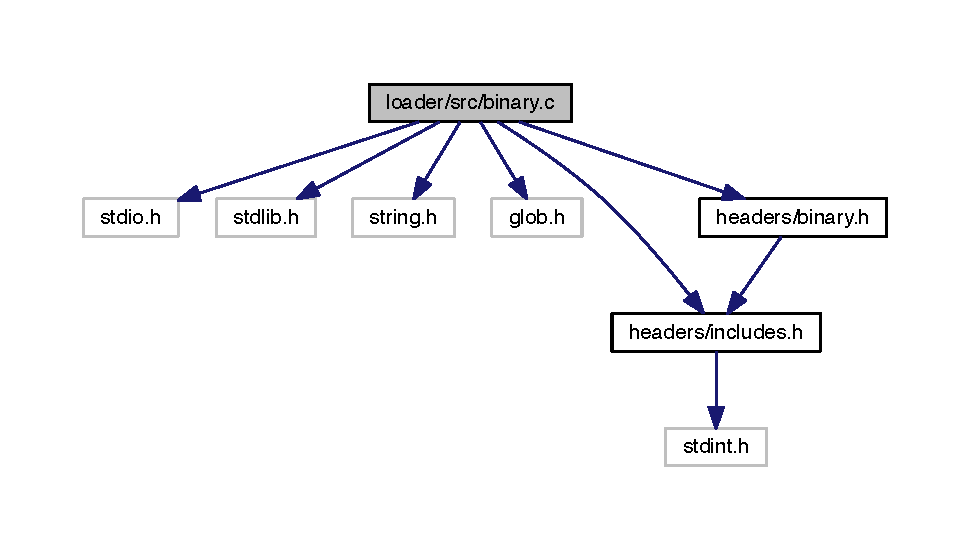
\includegraphics[width=350pt]{binary_8c__incl}
\end{center}
\end{figure}
\subsection*{Functions}
\begin{DoxyCompactItemize}
\item 
\hyperlink{loader_2src_2headers_2includes_8h_af492d2bddcb2befacb3aa03dcdf9aafd}{B\+O\+OL} \hyperlink{binary_8c_a4074aae87954abbb8dba12e44ccd9110}{binary\+\_\+init} (void)
\item 
struct \hyperlink{structbinary}{binary} $\ast$ \hyperlink{binary_8c_aaa1514c791103db3737fd7336a02bc70}{binary\+\_\+get\+\_\+by\+\_\+arch} (char $\ast$arch)
\end{DoxyCompactItemize}


\subsection{Function Documentation}
\index{binary.\+c@{binary.\+c}!binary\+\_\+get\+\_\+by\+\_\+arch@{binary\+\_\+get\+\_\+by\+\_\+arch}}
\index{binary\+\_\+get\+\_\+by\+\_\+arch@{binary\+\_\+get\+\_\+by\+\_\+arch}!binary.\+c@{binary.\+c}}
\subsubsection[{\texorpdfstring{binary\+\_\+get\+\_\+by\+\_\+arch(char $\ast$arch)}{binary_get_by_arch(char *arch)}}]{\setlength{\rightskip}{0pt plus 5cm}struct {\bf binary}$\ast$ binary\+\_\+get\+\_\+by\+\_\+arch (
\begin{DoxyParamCaption}
\item[{char $\ast$}]{arch}
\end{DoxyParamCaption}
)}\hypertarget{binary_8c_aaa1514c791103db3737fd7336a02bc70}{}\label{binary_8c_aaa1514c791103db3737fd7336a02bc70}


Definition at line 44 of file binary.\+c.



Here is the caller graph for this function\+:
\nopagebreak
\begin{figure}[H]
\begin{center}
\leavevmode
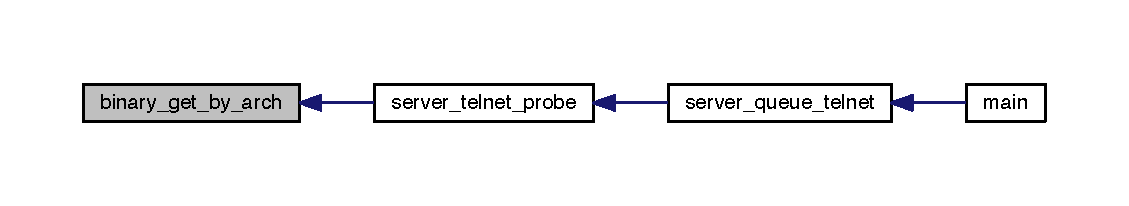
\includegraphics[width=350pt]{binary_8c_aaa1514c791103db3737fd7336a02bc70_icgraph}
\end{center}
\end{figure}


\index{binary.\+c@{binary.\+c}!binary\+\_\+init@{binary\+\_\+init}}
\index{binary\+\_\+init@{binary\+\_\+init}!binary.\+c@{binary.\+c}}
\subsubsection[{\texorpdfstring{binary\+\_\+init(void)}{binary_init(void)}}]{\setlength{\rightskip}{0pt plus 5cm}{\bf B\+O\+OL} binary\+\_\+init (
\begin{DoxyParamCaption}
\item[{void}]{}
\end{DoxyParamCaption}
)}\hypertarget{binary_8c_a4074aae87954abbb8dba12e44ccd9110}{}\label{binary_8c_a4074aae87954abbb8dba12e44ccd9110}


Definition at line 11 of file binary.\+c.



Here is the caller graph for this function\+:
\nopagebreak
\begin{figure}[H]
\begin{center}
\leavevmode
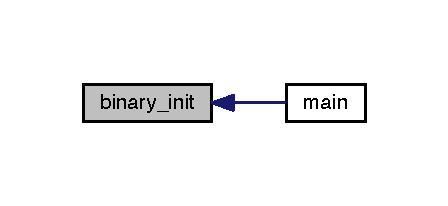
\includegraphics[width=215pt]{binary_8c_a4074aae87954abbb8dba12e44ccd9110_icgraph}
\end{center}
\end{figure}



\hypertarget{connection_8c}{}\section{loader/src/connection.c File Reference}
\label{connection_8c}\index{loader/src/connection.\+c@{loader/src/connection.\+c}}
{\ttfamily \#include $<$sys/socket.\+h$>$}\\*
{\ttfamily \#include $<$stdio.\+h$>$}\\*
{\ttfamily \#include $<$stdlib.\+h$>$}\\*
{\ttfamily \#include $<$string.\+h$>$}\\*
{\ttfamily \#include $<$time.\+h$>$}\\*
{\ttfamily \#include $<$pthread.\+h$>$}\\*
{\ttfamily \#include \char`\"{}headers/includes.\+h\char`\"{}}\\*
{\ttfamily \#include \char`\"{}headers/connection.\+h\char`\"{}}\\*
{\ttfamily \#include \char`\"{}headers/server.\+h\char`\"{}}\\*
{\ttfamily \#include \char`\"{}headers/binary.\+h\char`\"{}}\\*
{\ttfamily \#include \char`\"{}headers/util.\+h\char`\"{}}\\*
Include dependency graph for connection.\+c\+:
\nopagebreak
\begin{figure}[H]
\begin{center}
\leavevmode
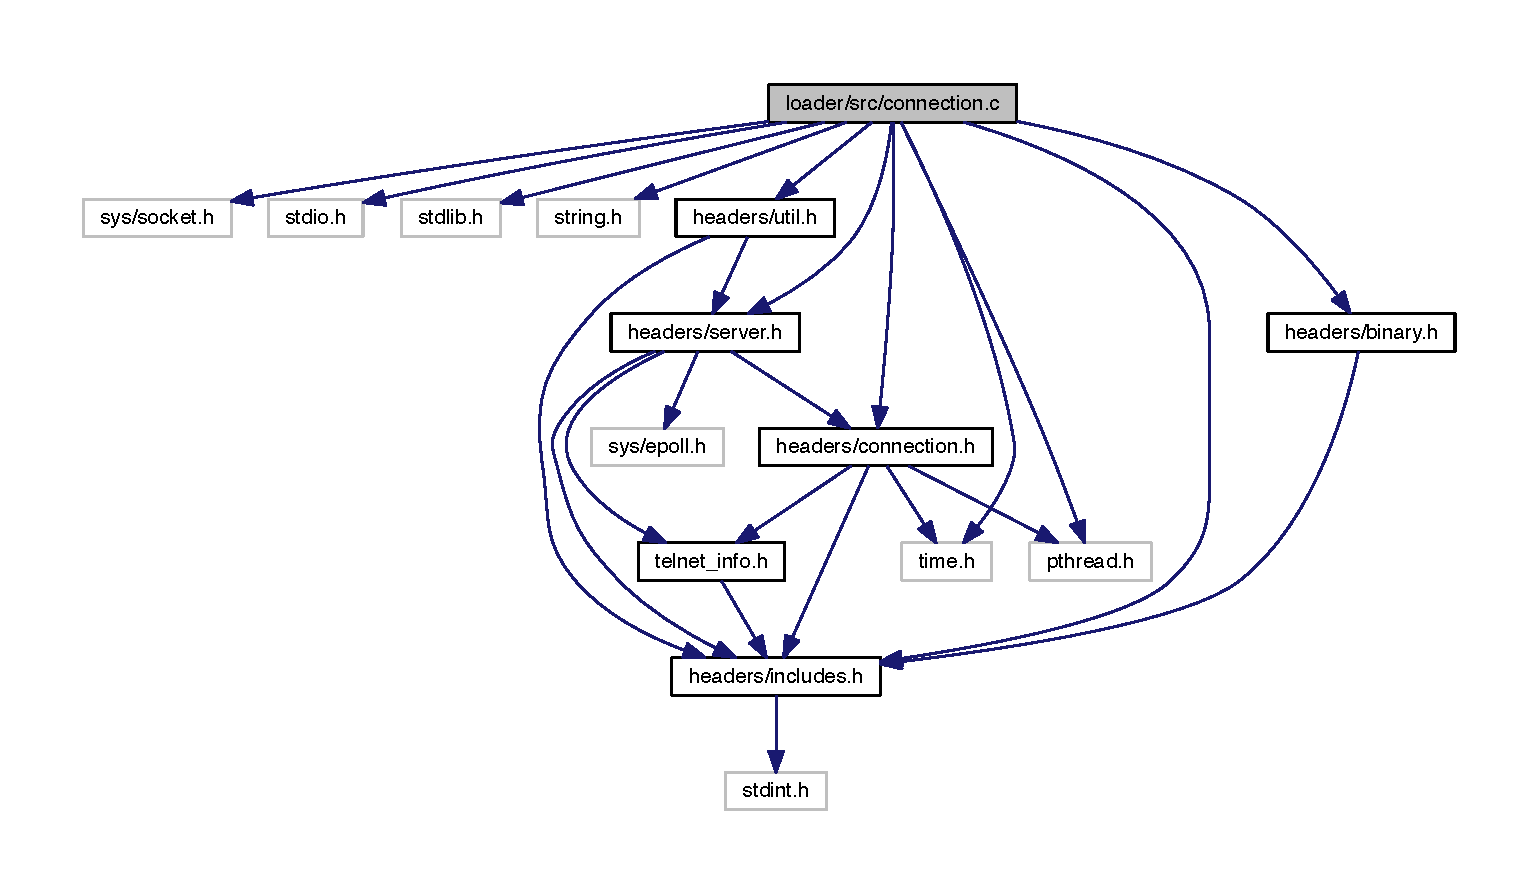
\includegraphics[width=350pt]{connection_8c__incl}
\end{center}
\end{figure}
\subsection*{Functions}
\begin{DoxyCompactItemize}
\item 
void \hyperlink{connection_8c_a162617f2f61ea5b24a221a6cc34d30e1}{connection\+\_\+open} (struct \hyperlink{structconnection}{connection} $\ast$conn)
\item 
void \hyperlink{connection_8c_abfa9e4a1232d41a78e5de0a510ed5752}{connection\+\_\+close} (struct \hyperlink{structconnection}{connection} $\ast$conn)
\item 
int \hyperlink{connection_8c_ac38d0bc660e02d86ce1dff3855004c09}{connection\+\_\+consume\+\_\+iacs} (struct \hyperlink{structconnection}{connection} $\ast$conn)
\item 
int \hyperlink{connection_8c_a8c48ff1129acb53db3b30a26fd9f6e48}{connection\+\_\+consume\+\_\+login\+\_\+prompt} (struct \hyperlink{structconnection}{connection} $\ast$conn)
\item 
int \hyperlink{connection_8c_a509389938f76d6277ffdb912ca8b4283}{connection\+\_\+consume\+\_\+password\+\_\+prompt} (struct \hyperlink{structconnection}{connection} $\ast$conn)
\item 
int \hyperlink{connection_8c_a52bc8c56bcf36ab89f034f7f6a7e77f1}{connection\+\_\+consume\+\_\+prompt} (struct \hyperlink{structconnection}{connection} $\ast$conn)
\item 
int \hyperlink{connection_8c_a6c25332d5f63d4d1256b55dd786e6295}{connection\+\_\+consume\+\_\+verify\+\_\+login} (struct \hyperlink{structconnection}{connection} $\ast$conn)
\item 
int \hyperlink{connection_8c_a9dbd998ccf8ca5a677d860ae6ea83344}{connection\+\_\+consume\+\_\+psoutput} (struct \hyperlink{structconnection}{connection} $\ast$conn)
\item 
int \hyperlink{connection_8c_a1cabdc0c7a73b41b2e51e515f61bf5db}{connection\+\_\+consume\+\_\+mounts} (struct \hyperlink{structconnection}{connection} $\ast$conn)
\item 
int \hyperlink{connection_8c_ab6b2144735ba2c7cedf9b93b4a1927db}{connection\+\_\+consume\+\_\+written\+\_\+dirs} (struct \hyperlink{structconnection}{connection} $\ast$conn)
\item 
int \hyperlink{connection_8c_aa5f67022eedf1d46da7efddad1864ecd}{connection\+\_\+consume\+\_\+copy\+\_\+op} (struct \hyperlink{structconnection}{connection} $\ast$conn)
\item 
int \hyperlink{connection_8c_ad724b4cf4d0bf51c69f33f6469ee4082}{connection\+\_\+consume\+\_\+arch} (struct \hyperlink{structconnection}{connection} $\ast$conn)
\item 
int \hyperlink{connection_8c_a8727b5c3aab5a5633d98ba86a15bbcfc}{connection\+\_\+consume\+\_\+arm\+\_\+subtype} (struct \hyperlink{structconnection}{connection} $\ast$conn)
\item 
int \hyperlink{connection_8c_a0ee0dff069c76ad003ae238270ac7c5d}{connection\+\_\+consume\+\_\+upload\+\_\+methods} (struct \hyperlink{structconnection}{connection} $\ast$conn)
\item 
int \hyperlink{connection_8c_a04dc8c68e7380236df79de3e1dc1d8bc}{connection\+\_\+upload\+\_\+echo} (struct \hyperlink{structconnection}{connection} $\ast$conn)
\item 
int \hyperlink{connection_8c_acb23df70b10e82b394c5aea71ce22a28}{connection\+\_\+upload\+\_\+wget} (struct \hyperlink{structconnection}{connection} $\ast$conn)
\item 
int \hyperlink{connection_8c_a409abf934163dd8108edb43f47abca81}{connection\+\_\+upload\+\_\+tftp} (struct \hyperlink{structconnection}{connection} $\ast$conn)
\item 
int \hyperlink{connection_8c_a6f9962c0bc2cedaf0de2814f4a5d4b17}{connection\+\_\+verify\+\_\+payload} (struct \hyperlink{structconnection}{connection} $\ast$conn)
\item 
int \hyperlink{connection_8c_a53ce7c6113c20961c61bbc6d64eae7c1}{connection\+\_\+consume\+\_\+cleanup} (struct \hyperlink{structconnection}{connection} $\ast$conn)
\end{DoxyCompactItemize}


\subsection{Function Documentation}
\index{connection.\+c@{connection.\+c}!connection\+\_\+close@{connection\+\_\+close}}
\index{connection\+\_\+close@{connection\+\_\+close}!connection.\+c@{connection.\+c}}
\subsubsection[{\texorpdfstring{connection\+\_\+close(struct connection $\ast$conn)}{connection_close(struct connection *conn)}}]{\setlength{\rightskip}{0pt plus 5cm}void connection\+\_\+close (
\begin{DoxyParamCaption}
\item[{struct {\bf connection} $\ast$}]{conn}
\end{DoxyParamCaption}
)}\hypertarget{connection_8c_abfa9e4a1232d41a78e5de0a510ed5752}{}\label{connection_8c_abfa9e4a1232d41a78e5de0a510ed5752}


Definition at line 33 of file connection.\+c.



Here is the caller graph for this function\+:
\nopagebreak
\begin{figure}[H]
\begin{center}
\leavevmode
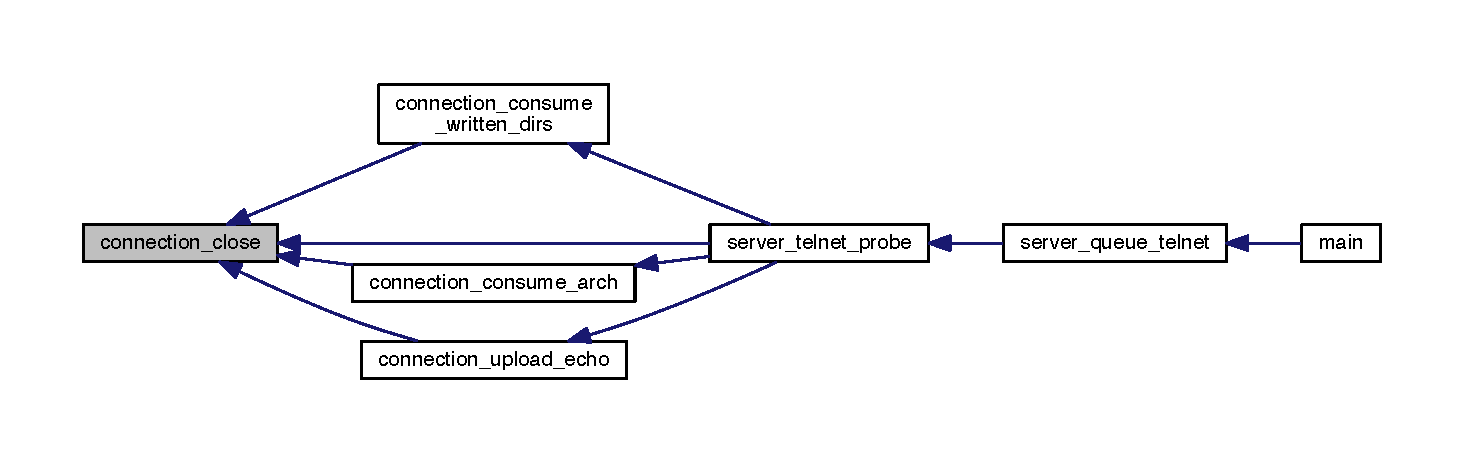
\includegraphics[width=350pt]{connection_8c_abfa9e4a1232d41a78e5de0a510ed5752_icgraph}
\end{center}
\end{figure}


\index{connection.\+c@{connection.\+c}!connection\+\_\+consume\+\_\+arch@{connection\+\_\+consume\+\_\+arch}}
\index{connection\+\_\+consume\+\_\+arch@{connection\+\_\+consume\+\_\+arch}!connection.\+c@{connection.\+c}}
\subsubsection[{\texorpdfstring{connection\+\_\+consume\+\_\+arch(struct connection $\ast$conn)}{connection_consume_arch(struct connection *conn)}}]{\setlength{\rightskip}{0pt plus 5cm}int connection\+\_\+consume\+\_\+arch (
\begin{DoxyParamCaption}
\item[{struct {\bf connection} $\ast$}]{conn}
\end{DoxyParamCaption}
)}\hypertarget{connection_8c_ad724b4cf4d0bf51c69f33f6469ee4082}{}\label{connection_8c_ad724b4cf4d0bf51c69f33f6469ee4082}


Definition at line 465 of file connection.\+c.



Here is the call graph for this function\+:
\nopagebreak
\begin{figure}[H]
\begin{center}
\leavevmode
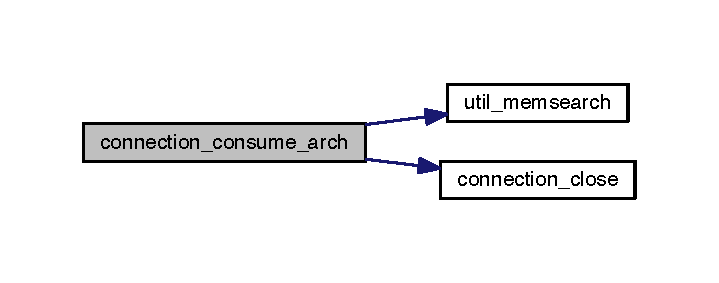
\includegraphics[width=345pt]{connection_8c_ad724b4cf4d0bf51c69f33f6469ee4082_cgraph}
\end{center}
\end{figure}




Here is the caller graph for this function\+:
\nopagebreak
\begin{figure}[H]
\begin{center}
\leavevmode
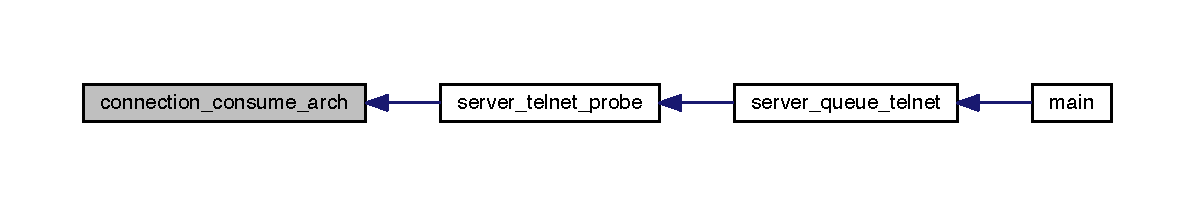
\includegraphics[width=350pt]{connection_8c_ad724b4cf4d0bf51c69f33f6469ee4082_icgraph}
\end{center}
\end{figure}


\index{connection.\+c@{connection.\+c}!connection\+\_\+consume\+\_\+arm\+\_\+subtype@{connection\+\_\+consume\+\_\+arm\+\_\+subtype}}
\index{connection\+\_\+consume\+\_\+arm\+\_\+subtype@{connection\+\_\+consume\+\_\+arm\+\_\+subtype}!connection.\+c@{connection.\+c}}
\subsubsection[{\texorpdfstring{connection\+\_\+consume\+\_\+arm\+\_\+subtype(struct connection $\ast$conn)}{connection_consume_arm_subtype(struct connection *conn)}}]{\setlength{\rightskip}{0pt plus 5cm}int connection\+\_\+consume\+\_\+arm\+\_\+subtype (
\begin{DoxyParamCaption}
\item[{struct {\bf connection} $\ast$}]{conn}
\end{DoxyParamCaption}
)}\hypertarget{connection_8c_a8727b5c3aab5a5633d98ba86a15bbcfc}{}\label{connection_8c_a8727b5c3aab5a5633d98ba86a15bbcfc}


Definition at line 538 of file connection.\+c.



Here is the call graph for this function\+:
\nopagebreak
\begin{figure}[H]
\begin{center}
\leavevmode
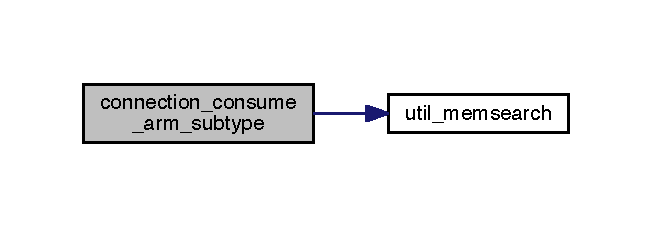
\includegraphics[width=313pt]{connection_8c_a8727b5c3aab5a5633d98ba86a15bbcfc_cgraph}
\end{center}
\end{figure}




Here is the caller graph for this function\+:
\nopagebreak
\begin{figure}[H]
\begin{center}
\leavevmode
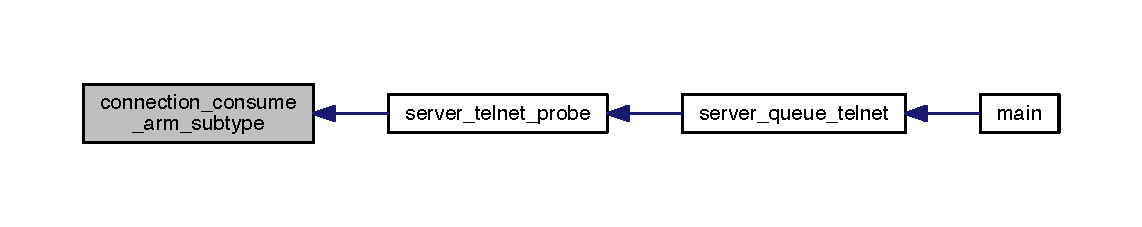
\includegraphics[width=350pt]{connection_8c_a8727b5c3aab5a5633d98ba86a15bbcfc_icgraph}
\end{center}
\end{figure}


\index{connection.\+c@{connection.\+c}!connection\+\_\+consume\+\_\+cleanup@{connection\+\_\+consume\+\_\+cleanup}}
\index{connection\+\_\+consume\+\_\+cleanup@{connection\+\_\+consume\+\_\+cleanup}!connection.\+c@{connection.\+c}}
\subsubsection[{\texorpdfstring{connection\+\_\+consume\+\_\+cleanup(struct connection $\ast$conn)}{connection_consume_cleanup(struct connection *conn)}}]{\setlength{\rightskip}{0pt plus 5cm}int connection\+\_\+consume\+\_\+cleanup (
\begin{DoxyParamCaption}
\item[{struct {\bf connection} $\ast$}]{conn}
\end{DoxyParamCaption}
)}\hypertarget{connection_8c_a53ce7c6113c20961c61bbc6d64eae7c1}{}\label{connection_8c_a53ce7c6113c20961c61bbc6d64eae7c1}


Definition at line 643 of file connection.\+c.



Here is the call graph for this function\+:
\nopagebreak
\begin{figure}[H]
\begin{center}
\leavevmode
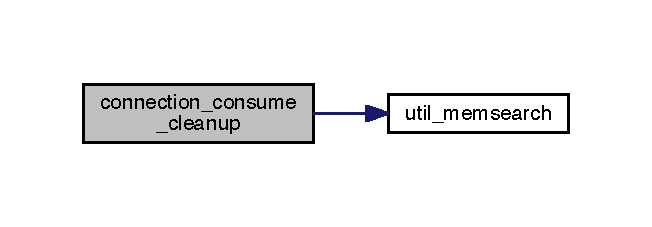
\includegraphics[width=313pt]{connection_8c_a53ce7c6113c20961c61bbc6d64eae7c1_cgraph}
\end{center}
\end{figure}




Here is the caller graph for this function\+:
\nopagebreak
\begin{figure}[H]
\begin{center}
\leavevmode
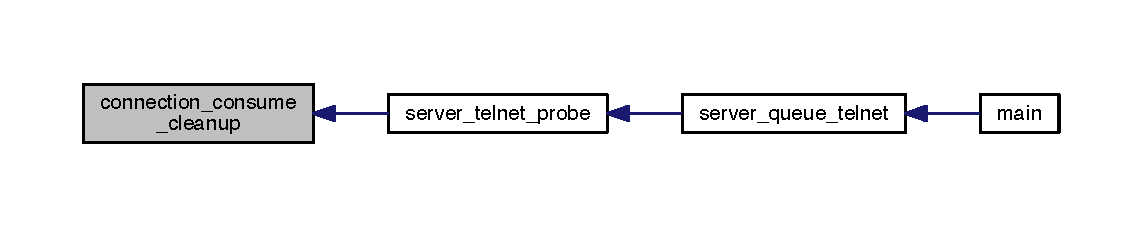
\includegraphics[width=350pt]{connection_8c_a53ce7c6113c20961c61bbc6d64eae7c1_icgraph}
\end{center}
\end{figure}


\index{connection.\+c@{connection.\+c}!connection\+\_\+consume\+\_\+copy\+\_\+op@{connection\+\_\+consume\+\_\+copy\+\_\+op}}
\index{connection\+\_\+consume\+\_\+copy\+\_\+op@{connection\+\_\+consume\+\_\+copy\+\_\+op}!connection.\+c@{connection.\+c}}
\subsubsection[{\texorpdfstring{connection\+\_\+consume\+\_\+copy\+\_\+op(struct connection $\ast$conn)}{connection_consume_copy_op(struct connection *conn)}}]{\setlength{\rightskip}{0pt plus 5cm}int connection\+\_\+consume\+\_\+copy\+\_\+op (
\begin{DoxyParamCaption}
\item[{struct {\bf connection} $\ast$}]{conn}
\end{DoxyParamCaption}
)}\hypertarget{connection_8c_aa5f67022eedf1d46da7efddad1864ecd}{}\label{connection_8c_aa5f67022eedf1d46da7efddad1864ecd}


Definition at line 456 of file connection.\+c.



Here is the call graph for this function\+:
\nopagebreak
\begin{figure}[H]
\begin{center}
\leavevmode
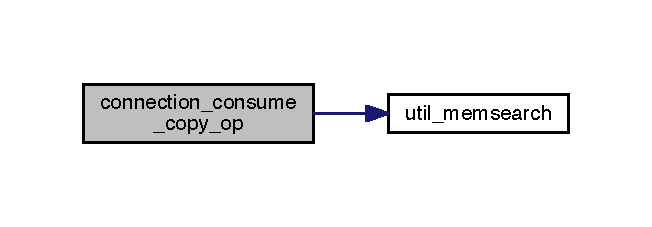
\includegraphics[width=313pt]{connection_8c_aa5f67022eedf1d46da7efddad1864ecd_cgraph}
\end{center}
\end{figure}




Here is the caller graph for this function\+:
\nopagebreak
\begin{figure}[H]
\begin{center}
\leavevmode
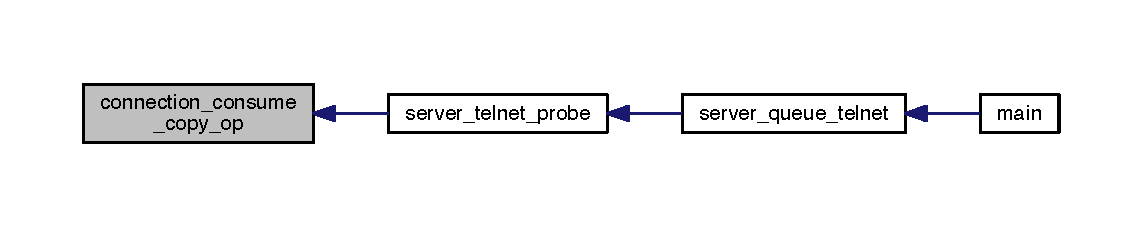
\includegraphics[width=350pt]{connection_8c_aa5f67022eedf1d46da7efddad1864ecd_icgraph}
\end{center}
\end{figure}


\index{connection.\+c@{connection.\+c}!connection\+\_\+consume\+\_\+iacs@{connection\+\_\+consume\+\_\+iacs}}
\index{connection\+\_\+consume\+\_\+iacs@{connection\+\_\+consume\+\_\+iacs}!connection.\+c@{connection.\+c}}
\subsubsection[{\texorpdfstring{connection\+\_\+consume\+\_\+iacs(struct connection $\ast$conn)}{connection_consume_iacs(struct connection *conn)}}]{\setlength{\rightskip}{0pt plus 5cm}int connection\+\_\+consume\+\_\+iacs (
\begin{DoxyParamCaption}
\item[{struct {\bf connection} $\ast$}]{conn}
\end{DoxyParamCaption}
)}\hypertarget{connection_8c_ac38d0bc660e02d86ce1dff3855004c09}{}\label{connection_8c_ac38d0bc660e02d86ce1dff3855004c09}


Definition at line 87 of file connection.\+c.



Here is the caller graph for this function\+:
\nopagebreak
\begin{figure}[H]
\begin{center}
\leavevmode
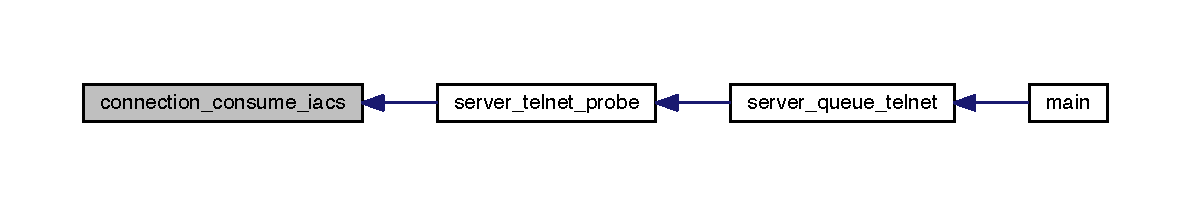
\includegraphics[width=350pt]{connection_8c_ac38d0bc660e02d86ce1dff3855004c09_icgraph}
\end{center}
\end{figure}


\index{connection.\+c@{connection.\+c}!connection\+\_\+consume\+\_\+login\+\_\+prompt@{connection\+\_\+consume\+\_\+login\+\_\+prompt}}
\index{connection\+\_\+consume\+\_\+login\+\_\+prompt@{connection\+\_\+consume\+\_\+login\+\_\+prompt}!connection.\+c@{connection.\+c}}
\subsubsection[{\texorpdfstring{connection\+\_\+consume\+\_\+login\+\_\+prompt(struct connection $\ast$conn)}{connection_consume_login_prompt(struct connection *conn)}}]{\setlength{\rightskip}{0pt plus 5cm}int connection\+\_\+consume\+\_\+login\+\_\+prompt (
\begin{DoxyParamCaption}
\item[{struct {\bf connection} $\ast$}]{conn}
\end{DoxyParamCaption}
)}\hypertarget{connection_8c_a8c48ff1129acb53db3b30a26fd9f6e48}{}\label{connection_8c_a8c48ff1129acb53db3b30a26fd9f6e48}


Definition at line 149 of file connection.\+c.



Here is the call graph for this function\+:
\nopagebreak
\begin{figure}[H]
\begin{center}
\leavevmode
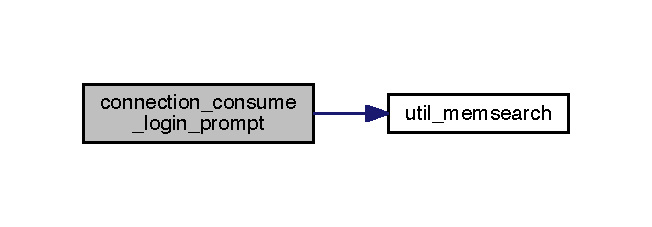
\includegraphics[width=313pt]{connection_8c_a8c48ff1129acb53db3b30a26fd9f6e48_cgraph}
\end{center}
\end{figure}




Here is the caller graph for this function\+:
\nopagebreak
\begin{figure}[H]
\begin{center}
\leavevmode
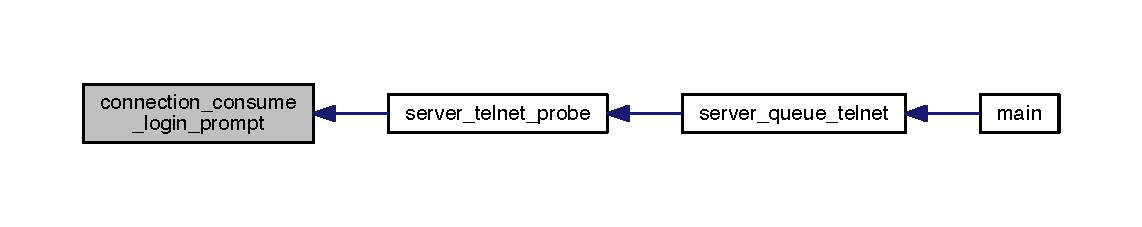
\includegraphics[width=350pt]{connection_8c_a8c48ff1129acb53db3b30a26fd9f6e48_icgraph}
\end{center}
\end{figure}


\index{connection.\+c@{connection.\+c}!connection\+\_\+consume\+\_\+mounts@{connection\+\_\+consume\+\_\+mounts}}
\index{connection\+\_\+consume\+\_\+mounts@{connection\+\_\+consume\+\_\+mounts}!connection.\+c@{connection.\+c}}
\subsubsection[{\texorpdfstring{connection\+\_\+consume\+\_\+mounts(struct connection $\ast$conn)}{connection_consume_mounts(struct connection *conn)}}]{\setlength{\rightskip}{0pt plus 5cm}int connection\+\_\+consume\+\_\+mounts (
\begin{DoxyParamCaption}
\item[{struct {\bf connection} $\ast$}]{conn}
\end{DoxyParamCaption}
)}\hypertarget{connection_8c_a1cabdc0c7a73b41b2e51e515f61bf5db}{}\label{connection_8c_a1cabdc0c7a73b41b2e51e515f61bf5db}


Definition at line 351 of file connection.\+c.



Here is the call graph for this function\+:
\nopagebreak
\begin{figure}[H]
\begin{center}
\leavevmode
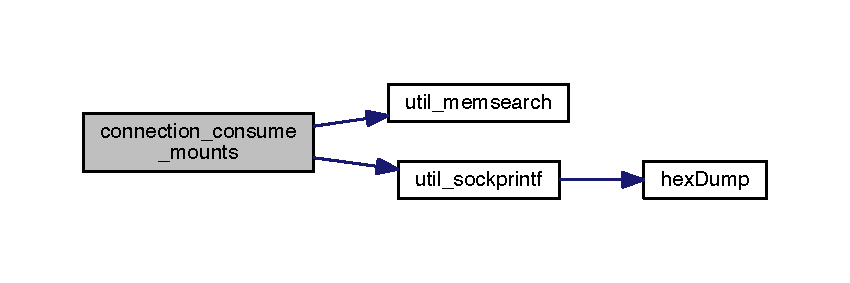
\includegraphics[width=350pt]{connection_8c_a1cabdc0c7a73b41b2e51e515f61bf5db_cgraph}
\end{center}
\end{figure}




Here is the caller graph for this function\+:
\nopagebreak
\begin{figure}[H]
\begin{center}
\leavevmode
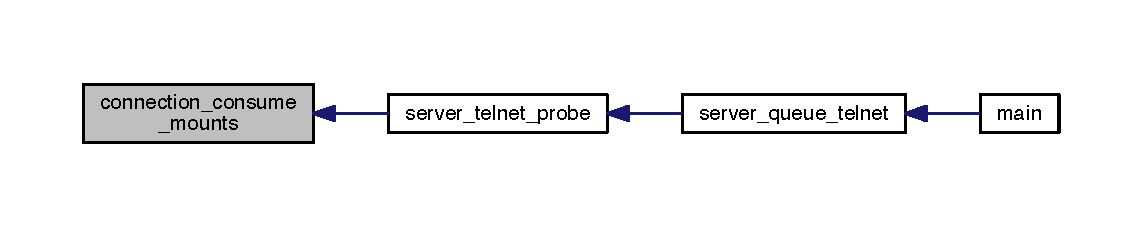
\includegraphics[width=350pt]{connection_8c_a1cabdc0c7a73b41b2e51e515f61bf5db_icgraph}
\end{center}
\end{figure}


\index{connection.\+c@{connection.\+c}!connection\+\_\+consume\+\_\+password\+\_\+prompt@{connection\+\_\+consume\+\_\+password\+\_\+prompt}}
\index{connection\+\_\+consume\+\_\+password\+\_\+prompt@{connection\+\_\+consume\+\_\+password\+\_\+prompt}!connection.\+c@{connection.\+c}}
\subsubsection[{\texorpdfstring{connection\+\_\+consume\+\_\+password\+\_\+prompt(struct connection $\ast$conn)}{connection_consume_password_prompt(struct connection *conn)}}]{\setlength{\rightskip}{0pt plus 5cm}int connection\+\_\+consume\+\_\+password\+\_\+prompt (
\begin{DoxyParamCaption}
\item[{struct {\bf connection} $\ast$}]{conn}
\end{DoxyParamCaption}
)}\hypertarget{connection_8c_a509389938f76d6277ffdb912ca8b4283}{}\label{connection_8c_a509389938f76d6277ffdb912ca8b4283}


Definition at line 182 of file connection.\+c.



Here is the call graph for this function\+:
\nopagebreak
\begin{figure}[H]
\begin{center}
\leavevmode
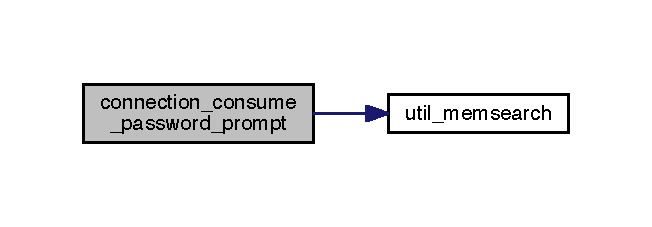
\includegraphics[width=313pt]{connection_8c_a509389938f76d6277ffdb912ca8b4283_cgraph}
\end{center}
\end{figure}




Here is the caller graph for this function\+:
\nopagebreak
\begin{figure}[H]
\begin{center}
\leavevmode
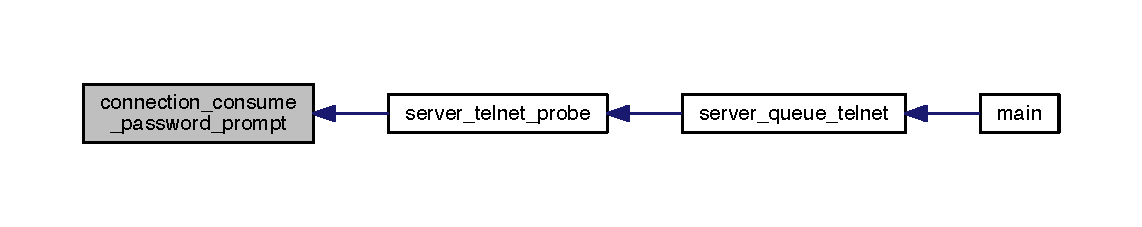
\includegraphics[width=350pt]{connection_8c_a509389938f76d6277ffdb912ca8b4283_icgraph}
\end{center}
\end{figure}


\index{connection.\+c@{connection.\+c}!connection\+\_\+consume\+\_\+prompt@{connection\+\_\+consume\+\_\+prompt}}
\index{connection\+\_\+consume\+\_\+prompt@{connection\+\_\+consume\+\_\+prompt}!connection.\+c@{connection.\+c}}
\subsubsection[{\texorpdfstring{connection\+\_\+consume\+\_\+prompt(struct connection $\ast$conn)}{connection_consume_prompt(struct connection *conn)}}]{\setlength{\rightskip}{0pt plus 5cm}int connection\+\_\+consume\+\_\+prompt (
\begin{DoxyParamCaption}
\item[{struct {\bf connection} $\ast$}]{conn}
\end{DoxyParamCaption}
)}\hypertarget{connection_8c_a52bc8c56bcf36ab89f034f7f6a7e77f1}{}\label{connection_8c_a52bc8c56bcf36ab89f034f7f6a7e77f1}


Definition at line 213 of file connection.\+c.



Here is the caller graph for this function\+:
\nopagebreak
\begin{figure}[H]
\begin{center}
\leavevmode
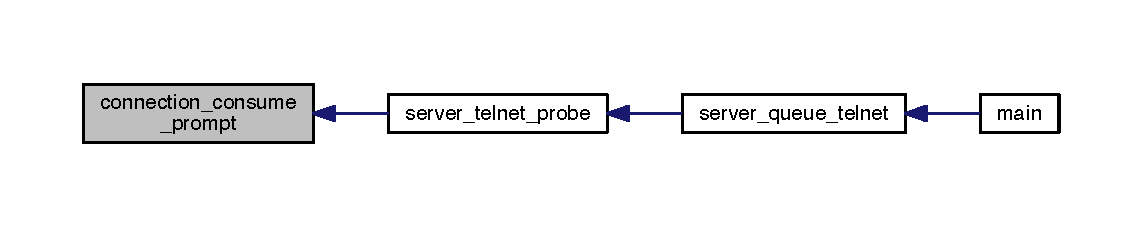
\includegraphics[width=350pt]{connection_8c_a52bc8c56bcf36ab89f034f7f6a7e77f1_icgraph}
\end{center}
\end{figure}


\index{connection.\+c@{connection.\+c}!connection\+\_\+consume\+\_\+psoutput@{connection\+\_\+consume\+\_\+psoutput}}
\index{connection\+\_\+consume\+\_\+psoutput@{connection\+\_\+consume\+\_\+psoutput}!connection.\+c@{connection.\+c}}
\subsubsection[{\texorpdfstring{connection\+\_\+consume\+\_\+psoutput(struct connection $\ast$conn)}{connection_consume_psoutput(struct connection *conn)}}]{\setlength{\rightskip}{0pt plus 5cm}int connection\+\_\+consume\+\_\+psoutput (
\begin{DoxyParamCaption}
\item[{struct {\bf connection} $\ast$}]{conn}
\end{DoxyParamCaption}
)}\hypertarget{connection_8c_a9dbd998ccf8ca5a677d860ae6ea83344}{}\label{connection_8c_a9dbd998ccf8ca5a677d860ae6ea83344}


Definition at line 246 of file connection.\+c.



Here is the call graph for this function\+:
\nopagebreak
\begin{figure}[H]
\begin{center}
\leavevmode
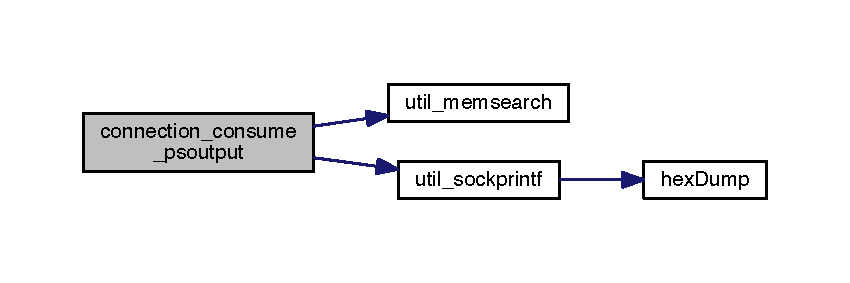
\includegraphics[width=350pt]{connection_8c_a9dbd998ccf8ca5a677d860ae6ea83344_cgraph}
\end{center}
\end{figure}




Here is the caller graph for this function\+:
\nopagebreak
\begin{figure}[H]
\begin{center}
\leavevmode
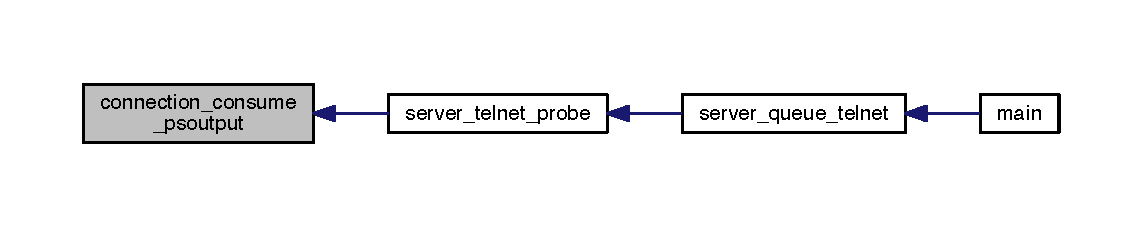
\includegraphics[width=350pt]{connection_8c_a9dbd998ccf8ca5a677d860ae6ea83344_icgraph}
\end{center}
\end{figure}


\index{connection.\+c@{connection.\+c}!connection\+\_\+consume\+\_\+upload\+\_\+methods@{connection\+\_\+consume\+\_\+upload\+\_\+methods}}
\index{connection\+\_\+consume\+\_\+upload\+\_\+methods@{connection\+\_\+consume\+\_\+upload\+\_\+methods}!connection.\+c@{connection.\+c}}
\subsubsection[{\texorpdfstring{connection\+\_\+consume\+\_\+upload\+\_\+methods(struct connection $\ast$conn)}{connection_consume_upload_methods(struct connection *conn)}}]{\setlength{\rightskip}{0pt plus 5cm}int connection\+\_\+consume\+\_\+upload\+\_\+methods (
\begin{DoxyParamCaption}
\item[{struct {\bf connection} $\ast$}]{conn}
\end{DoxyParamCaption}
)}\hypertarget{connection_8c_a0ee0dff069c76ad003ae238270ac7c5d}{}\label{connection_8c_a0ee0dff069c76ad003ae238270ac7c5d}


Definition at line 556 of file connection.\+c.



Here is the call graph for this function\+:
\nopagebreak
\begin{figure}[H]
\begin{center}
\leavevmode
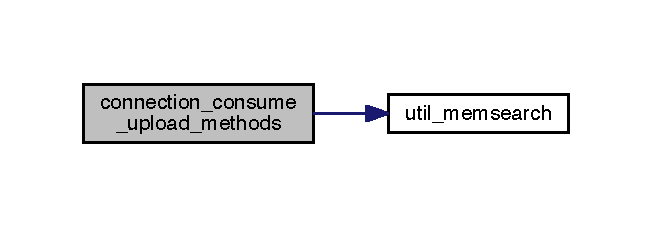
\includegraphics[width=313pt]{connection_8c_a0ee0dff069c76ad003ae238270ac7c5d_cgraph}
\end{center}
\end{figure}




Here is the caller graph for this function\+:
\nopagebreak
\begin{figure}[H]
\begin{center}
\leavevmode
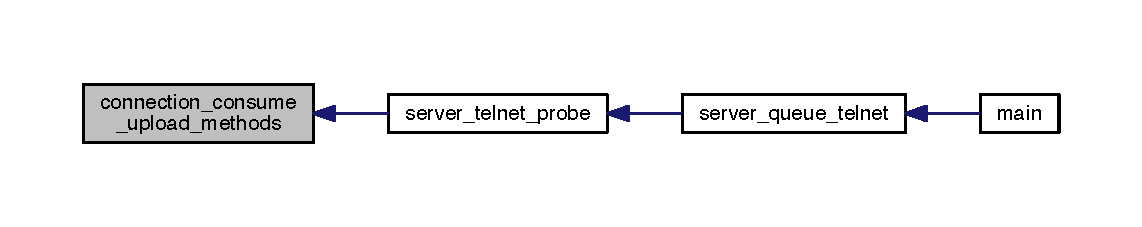
\includegraphics[width=350pt]{connection_8c_a0ee0dff069c76ad003ae238270ac7c5d_icgraph}
\end{center}
\end{figure}


\index{connection.\+c@{connection.\+c}!connection\+\_\+consume\+\_\+verify\+\_\+login@{connection\+\_\+consume\+\_\+verify\+\_\+login}}
\index{connection\+\_\+consume\+\_\+verify\+\_\+login@{connection\+\_\+consume\+\_\+verify\+\_\+login}!connection.\+c@{connection.\+c}}
\subsubsection[{\texorpdfstring{connection\+\_\+consume\+\_\+verify\+\_\+login(struct connection $\ast$conn)}{connection_consume_verify_login(struct connection *conn)}}]{\setlength{\rightskip}{0pt plus 5cm}int connection\+\_\+consume\+\_\+verify\+\_\+login (
\begin{DoxyParamCaption}
\item[{struct {\bf connection} $\ast$}]{conn}
\end{DoxyParamCaption}
)}\hypertarget{connection_8c_a6c25332d5f63d4d1256b55dd786e6295}{}\label{connection_8c_a6c25332d5f63d4d1256b55dd786e6295}


Definition at line 236 of file connection.\+c.



Here is the call graph for this function\+:
\nopagebreak
\begin{figure}[H]
\begin{center}
\leavevmode
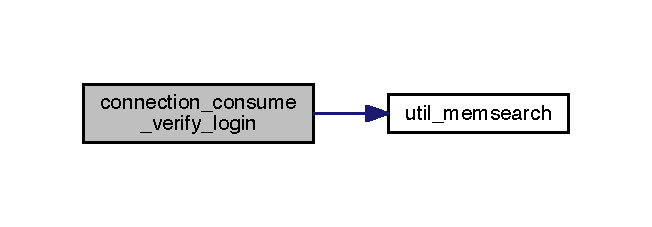
\includegraphics[width=313pt]{connection_8c_a6c25332d5f63d4d1256b55dd786e6295_cgraph}
\end{center}
\end{figure}




Here is the caller graph for this function\+:
\nopagebreak
\begin{figure}[H]
\begin{center}
\leavevmode
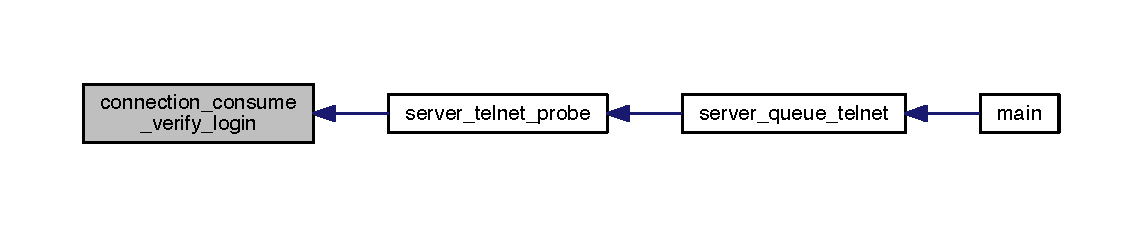
\includegraphics[width=350pt]{connection_8c_a6c25332d5f63d4d1256b55dd786e6295_icgraph}
\end{center}
\end{figure}


\index{connection.\+c@{connection.\+c}!connection\+\_\+consume\+\_\+written\+\_\+dirs@{connection\+\_\+consume\+\_\+written\+\_\+dirs}}
\index{connection\+\_\+consume\+\_\+written\+\_\+dirs@{connection\+\_\+consume\+\_\+written\+\_\+dirs}!connection.\+c@{connection.\+c}}
\subsubsection[{\texorpdfstring{connection\+\_\+consume\+\_\+written\+\_\+dirs(struct connection $\ast$conn)}{connection_consume_written_dirs(struct connection *conn)}}]{\setlength{\rightskip}{0pt plus 5cm}int connection\+\_\+consume\+\_\+written\+\_\+dirs (
\begin{DoxyParamCaption}
\item[{struct {\bf connection} $\ast$}]{conn}
\end{DoxyParamCaption}
)}\hypertarget{connection_8c_ab6b2144735ba2c7cedf9b93b4a1927db}{}\label{connection_8c_ab6b2144735ba2c7cedf9b93b4a1927db}


Definition at line 414 of file connection.\+c.



Here is the call graph for this function\+:
\nopagebreak
\begin{figure}[H]
\begin{center}
\leavevmode
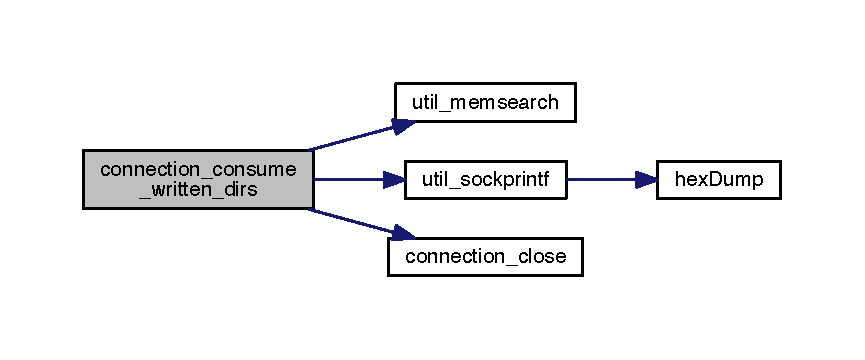
\includegraphics[width=350pt]{connection_8c_ab6b2144735ba2c7cedf9b93b4a1927db_cgraph}
\end{center}
\end{figure}




Here is the caller graph for this function\+:
\nopagebreak
\begin{figure}[H]
\begin{center}
\leavevmode
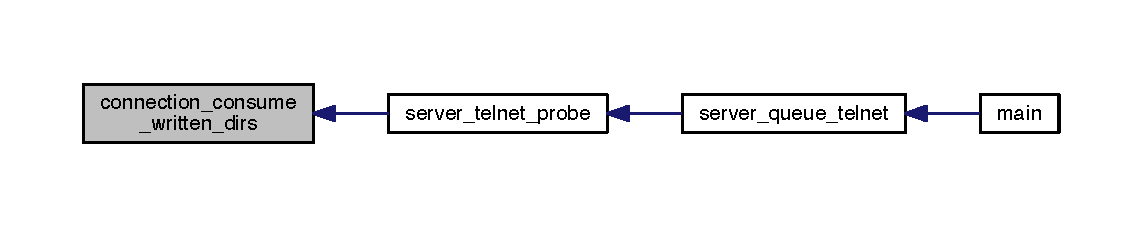
\includegraphics[width=350pt]{connection_8c_ab6b2144735ba2c7cedf9b93b4a1927db_icgraph}
\end{center}
\end{figure}


\index{connection.\+c@{connection.\+c}!connection\+\_\+open@{connection\+\_\+open}}
\index{connection\+\_\+open@{connection\+\_\+open}!connection.\+c@{connection.\+c}}
\subsubsection[{\texorpdfstring{connection\+\_\+open(struct connection $\ast$conn)}{connection_open(struct connection *conn)}}]{\setlength{\rightskip}{0pt plus 5cm}void connection\+\_\+open (
\begin{DoxyParamCaption}
\item[{struct {\bf connection} $\ast$}]{conn}
\end{DoxyParamCaption}
)}\hypertarget{connection_8c_a162617f2f61ea5b24a221a6cc34d30e1}{}\label{connection_8c_a162617f2f61ea5b24a221a6cc34d30e1}


Definition at line 13 of file connection.\+c.



Here is the caller graph for this function\+:
\nopagebreak
\begin{figure}[H]
\begin{center}
\leavevmode
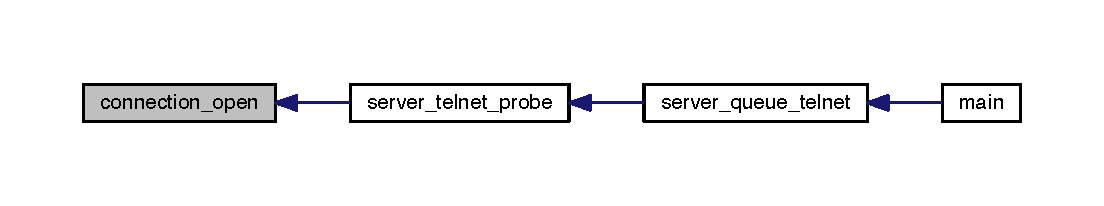
\includegraphics[width=350pt]{connection_8c_a162617f2f61ea5b24a221a6cc34d30e1_icgraph}
\end{center}
\end{figure}


\index{connection.\+c@{connection.\+c}!connection\+\_\+upload\+\_\+echo@{connection\+\_\+upload\+\_\+echo}}
\index{connection\+\_\+upload\+\_\+echo@{connection\+\_\+upload\+\_\+echo}!connection.\+c@{connection.\+c}}
\subsubsection[{\texorpdfstring{connection\+\_\+upload\+\_\+echo(struct connection $\ast$conn)}{connection_upload_echo(struct connection *conn)}}]{\setlength{\rightskip}{0pt plus 5cm}int connection\+\_\+upload\+\_\+echo (
\begin{DoxyParamCaption}
\item[{struct {\bf connection} $\ast$}]{conn}
\end{DoxyParamCaption}
)}\hypertarget{connection_8c_a04dc8c68e7380236df79de3e1dc1d8bc}{}\label{connection_8c_a04dc8c68e7380236df79de3e1dc1d8bc}


Definition at line 573 of file connection.\+c.



Here is the call graph for this function\+:
\nopagebreak
\begin{figure}[H]
\begin{center}
\leavevmode
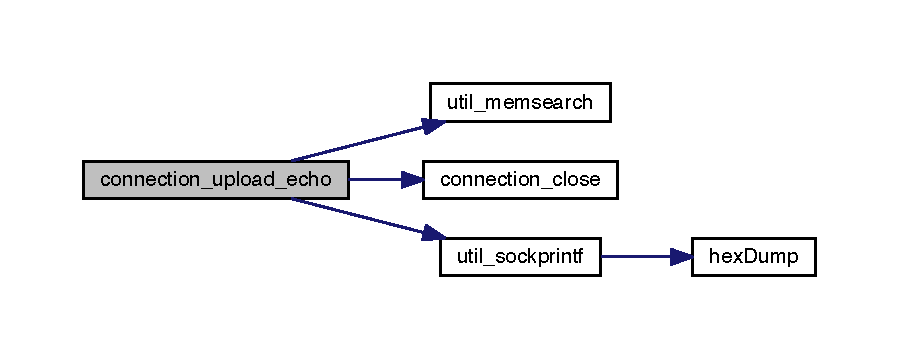
\includegraphics[width=350pt]{connection_8c_a04dc8c68e7380236df79de3e1dc1d8bc_cgraph}
\end{center}
\end{figure}




Here is the caller graph for this function\+:
\nopagebreak
\begin{figure}[H]
\begin{center}
\leavevmode
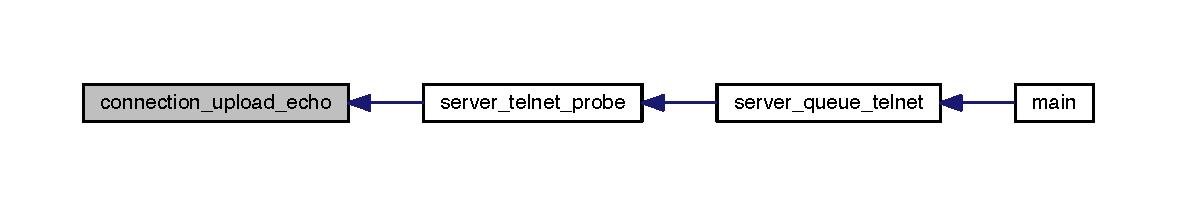
\includegraphics[width=350pt]{connection_8c_a04dc8c68e7380236df79de3e1dc1d8bc_icgraph}
\end{center}
\end{figure}


\index{connection.\+c@{connection.\+c}!connection\+\_\+upload\+\_\+tftp@{connection\+\_\+upload\+\_\+tftp}}
\index{connection\+\_\+upload\+\_\+tftp@{connection\+\_\+upload\+\_\+tftp}!connection.\+c@{connection.\+c}}
\subsubsection[{\texorpdfstring{connection\+\_\+upload\+\_\+tftp(struct connection $\ast$conn)}{connection_upload_tftp(struct connection *conn)}}]{\setlength{\rightskip}{0pt plus 5cm}int connection\+\_\+upload\+\_\+tftp (
\begin{DoxyParamCaption}
\item[{struct {\bf connection} $\ast$}]{conn}
\end{DoxyParamCaption}
)}\hypertarget{connection_8c_a409abf934163dd8108edb43f47abca81}{}\label{connection_8c_a409abf934163dd8108edb43f47abca81}


Definition at line 611 of file connection.\+c.



Here is the call graph for this function\+:
\nopagebreak
\begin{figure}[H]
\begin{center}
\leavevmode
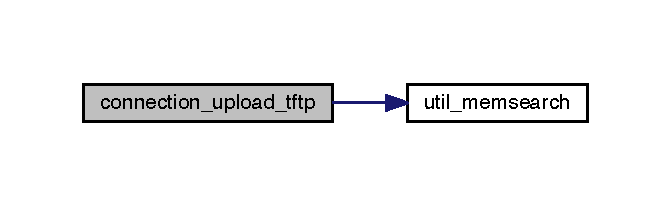
\includegraphics[width=322pt]{connection_8c_a409abf934163dd8108edb43f47abca81_cgraph}
\end{center}
\end{figure}




Here is the caller graph for this function\+:
\nopagebreak
\begin{figure}[H]
\begin{center}
\leavevmode
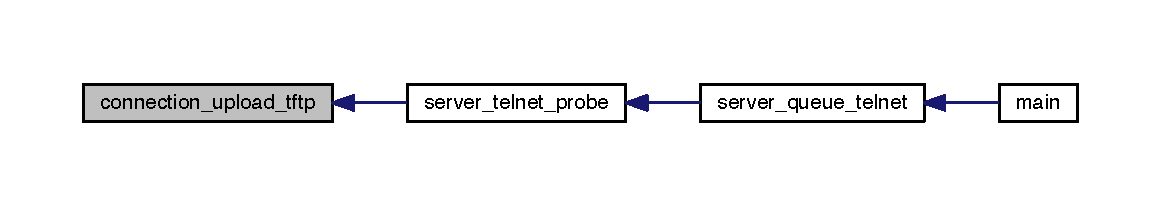
\includegraphics[width=350pt]{connection_8c_a409abf934163dd8108edb43f47abca81_icgraph}
\end{center}
\end{figure}


\index{connection.\+c@{connection.\+c}!connection\+\_\+upload\+\_\+wget@{connection\+\_\+upload\+\_\+wget}}
\index{connection\+\_\+upload\+\_\+wget@{connection\+\_\+upload\+\_\+wget}!connection.\+c@{connection.\+c}}
\subsubsection[{\texorpdfstring{connection\+\_\+upload\+\_\+wget(struct connection $\ast$conn)}{connection_upload_wget(struct connection *conn)}}]{\setlength{\rightskip}{0pt plus 5cm}int connection\+\_\+upload\+\_\+wget (
\begin{DoxyParamCaption}
\item[{struct {\bf connection} $\ast$}]{conn}
\end{DoxyParamCaption}
)}\hypertarget{connection_8c_acb23df70b10e82b394c5aea71ce22a28}{}\label{connection_8c_acb23df70b10e82b394c5aea71ce22a28}


Definition at line 601 of file connection.\+c.



Here is the call graph for this function\+:
\nopagebreak
\begin{figure}[H]
\begin{center}
\leavevmode
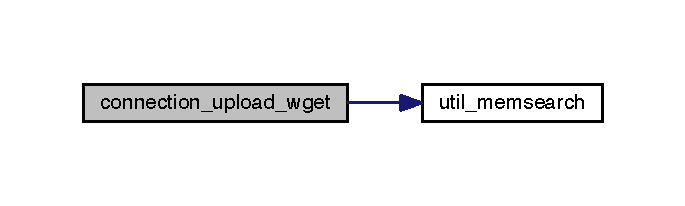
\includegraphics[width=329pt]{connection_8c_acb23df70b10e82b394c5aea71ce22a28_cgraph}
\end{center}
\end{figure}




Here is the caller graph for this function\+:
\nopagebreak
\begin{figure}[H]
\begin{center}
\leavevmode
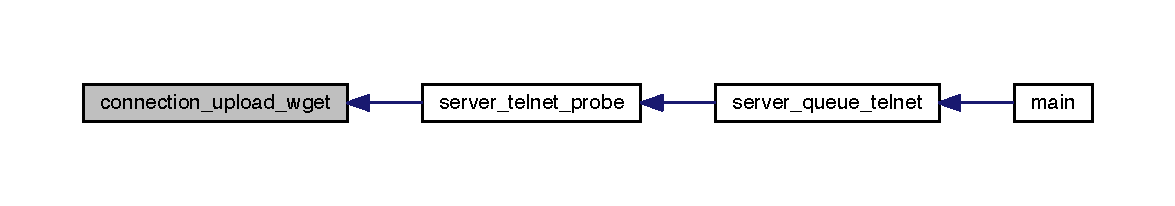
\includegraphics[width=350pt]{connection_8c_acb23df70b10e82b394c5aea71ce22a28_icgraph}
\end{center}
\end{figure}


\index{connection.\+c@{connection.\+c}!connection\+\_\+verify\+\_\+payload@{connection\+\_\+verify\+\_\+payload}}
\index{connection\+\_\+verify\+\_\+payload@{connection\+\_\+verify\+\_\+payload}!connection.\+c@{connection.\+c}}
\subsubsection[{\texorpdfstring{connection\+\_\+verify\+\_\+payload(struct connection $\ast$conn)}{connection_verify_payload(struct connection *conn)}}]{\setlength{\rightskip}{0pt plus 5cm}int connection\+\_\+verify\+\_\+payload (
\begin{DoxyParamCaption}
\item[{struct {\bf connection} $\ast$}]{conn}
\end{DoxyParamCaption}
)}\hypertarget{connection_8c_a6f9962c0bc2cedaf0de2814f4a5d4b17}{}\label{connection_8c_a6f9962c0bc2cedaf0de2814f4a5d4b17}


Definition at line 630 of file connection.\+c.



Here is the call graph for this function\+:
\nopagebreak
\begin{figure}[H]
\begin{center}
\leavevmode
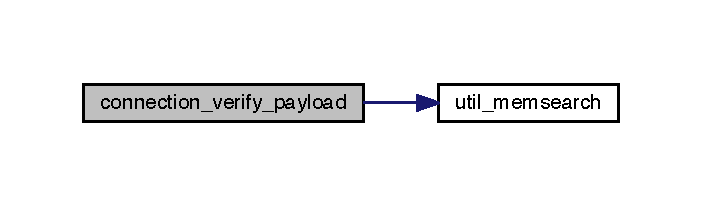
\includegraphics[width=337pt]{connection_8c_a6f9962c0bc2cedaf0de2814f4a5d4b17_cgraph}
\end{center}
\end{figure}




Here is the caller graph for this function\+:
\nopagebreak
\begin{figure}[H]
\begin{center}
\leavevmode
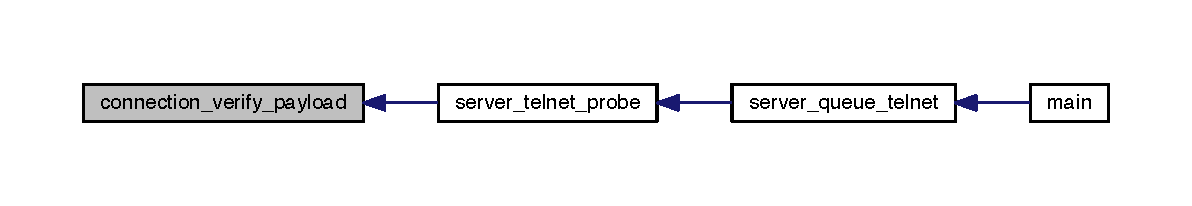
\includegraphics[width=350pt]{connection_8c_a6f9962c0bc2cedaf0de2814f4a5d4b17_icgraph}
\end{center}
\end{figure}



\hypertarget{binary_8h}{}\section{loader/src/headers/binary.h File Reference}
\label{binary_8h}\index{loader/src/headers/binary.\+h@{loader/src/headers/binary.\+h}}
{\ttfamily \#include \char`\"{}includes.\+h\char`\"{}}\\*
Include dependency graph for binary.\+h\+:
\nopagebreak
\begin{figure}[H]
\begin{center}
\leavevmode
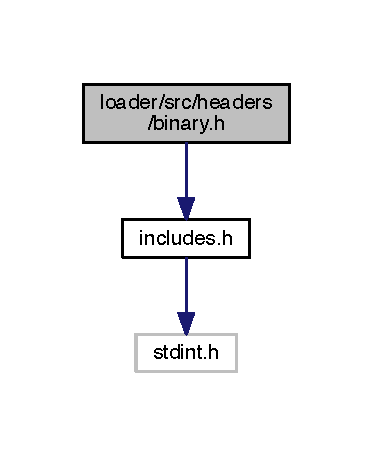
\includegraphics[width=179pt]{binary_8h__incl}
\end{center}
\end{figure}
This graph shows which files directly or indirectly include this file\+:
\nopagebreak
\begin{figure}[H]
\begin{center}
\leavevmode
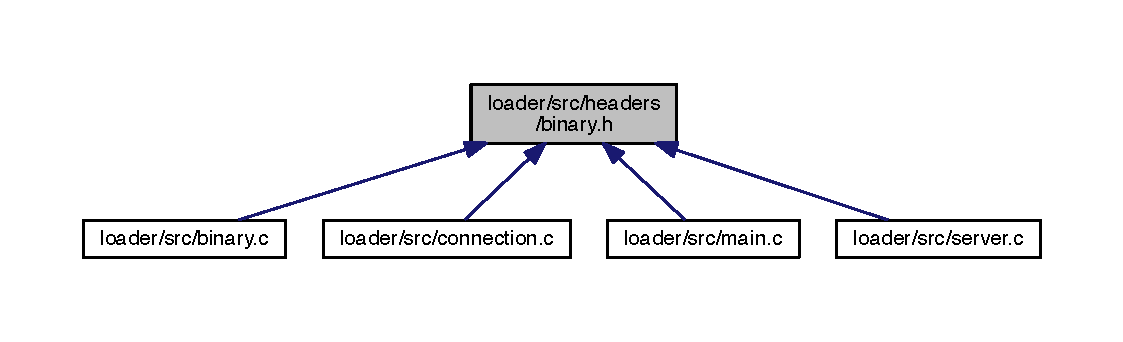
\includegraphics[width=350pt]{binary_8h__dep__incl}
\end{center}
\end{figure}
\subsection*{Data Structures}
\begin{DoxyCompactItemize}
\item 
struct \hyperlink{structbinary}{binary}
\end{DoxyCompactItemize}
\subsection*{Macros}
\begin{DoxyCompactItemize}
\item 
\#define \hyperlink{binary_8h_ab9d82cae2dc04046089e117a9ce34887}{B\+I\+N\+A\+R\+Y\+\_\+\+B\+Y\+T\+E\+S\+\_\+\+P\+E\+R\+\_\+\+E\+C\+H\+O\+L\+I\+NE}~128
\end{DoxyCompactItemize}
\subsection*{Functions}
\begin{DoxyCompactItemize}
\item 
\hyperlink{loader_2src_2headers_2includes_8h_af492d2bddcb2befacb3aa03dcdf9aafd}{B\+O\+OL} \hyperlink{binary_8h_a4074aae87954abbb8dba12e44ccd9110}{binary\+\_\+init} (void)
\item 
struct \hyperlink{structbinary}{binary} $\ast$ \hyperlink{binary_8h_aaa1514c791103db3737fd7336a02bc70}{binary\+\_\+get\+\_\+by\+\_\+arch} (char $\ast$arch)
\end{DoxyCompactItemize}


\subsection{Macro Definition Documentation}
\index{binary.\+h@{binary.\+h}!B\+I\+N\+A\+R\+Y\+\_\+\+B\+Y\+T\+E\+S\+\_\+\+P\+E\+R\+\_\+\+E\+C\+H\+O\+L\+I\+NE@{B\+I\+N\+A\+R\+Y\+\_\+\+B\+Y\+T\+E\+S\+\_\+\+P\+E\+R\+\_\+\+E\+C\+H\+O\+L\+I\+NE}}
\index{B\+I\+N\+A\+R\+Y\+\_\+\+B\+Y\+T\+E\+S\+\_\+\+P\+E\+R\+\_\+\+E\+C\+H\+O\+L\+I\+NE@{B\+I\+N\+A\+R\+Y\+\_\+\+B\+Y\+T\+E\+S\+\_\+\+P\+E\+R\+\_\+\+E\+C\+H\+O\+L\+I\+NE}!binary.\+h@{binary.\+h}}
\subsubsection[{\texorpdfstring{B\+I\+N\+A\+R\+Y\+\_\+\+B\+Y\+T\+E\+S\+\_\+\+P\+E\+R\+\_\+\+E\+C\+H\+O\+L\+I\+NE}{BINARY_BYTES_PER_ECHOLINE}}]{\setlength{\rightskip}{0pt plus 5cm}\#define B\+I\+N\+A\+R\+Y\+\_\+\+B\+Y\+T\+E\+S\+\_\+\+P\+E\+R\+\_\+\+E\+C\+H\+O\+L\+I\+NE~128}\hypertarget{binary_8h_ab9d82cae2dc04046089e117a9ce34887}{}\label{binary_8h_ab9d82cae2dc04046089e117a9ce34887}


Definition at line 5 of file binary.\+h.



\subsection{Function Documentation}
\index{binary.\+h@{binary.\+h}!binary\+\_\+get\+\_\+by\+\_\+arch@{binary\+\_\+get\+\_\+by\+\_\+arch}}
\index{binary\+\_\+get\+\_\+by\+\_\+arch@{binary\+\_\+get\+\_\+by\+\_\+arch}!binary.\+h@{binary.\+h}}
\subsubsection[{\texorpdfstring{binary\+\_\+get\+\_\+by\+\_\+arch(char $\ast$arch)}{binary_get_by_arch(char *arch)}}]{\setlength{\rightskip}{0pt plus 5cm}struct {\bf binary}$\ast$ binary\+\_\+get\+\_\+by\+\_\+arch (
\begin{DoxyParamCaption}
\item[{char $\ast$}]{arch}
\end{DoxyParamCaption}
)}\hypertarget{binary_8h_aaa1514c791103db3737fd7336a02bc70}{}\label{binary_8h_aaa1514c791103db3737fd7336a02bc70}


Definition at line 44 of file binary.\+c.



Here is the caller graph for this function\+:
\nopagebreak
\begin{figure}[H]
\begin{center}
\leavevmode
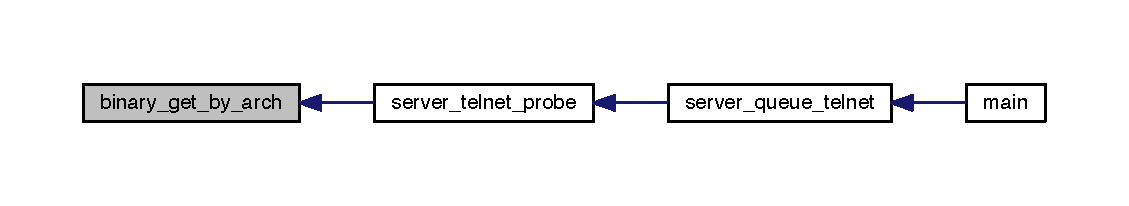
\includegraphics[width=350pt]{binary_8h_aaa1514c791103db3737fd7336a02bc70_icgraph}
\end{center}
\end{figure}


\index{binary.\+h@{binary.\+h}!binary\+\_\+init@{binary\+\_\+init}}
\index{binary\+\_\+init@{binary\+\_\+init}!binary.\+h@{binary.\+h}}
\subsubsection[{\texorpdfstring{binary\+\_\+init(void)}{binary_init(void)}}]{\setlength{\rightskip}{0pt plus 5cm}{\bf B\+O\+OL} binary\+\_\+init (
\begin{DoxyParamCaption}
\item[{void}]{}
\end{DoxyParamCaption}
)}\hypertarget{binary_8h_a4074aae87954abbb8dba12e44ccd9110}{}\label{binary_8h_a4074aae87954abbb8dba12e44ccd9110}


Definition at line 11 of file binary.\+c.



Here is the caller graph for this function\+:
\nopagebreak
\begin{figure}[H]
\begin{center}
\leavevmode
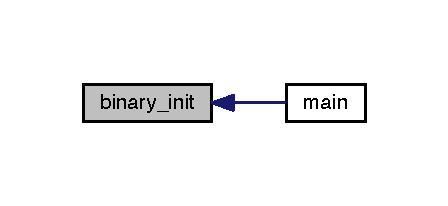
\includegraphics[width=215pt]{binary_8h_a4074aae87954abbb8dba12e44ccd9110_icgraph}
\end{center}
\end{figure}



\hypertarget{connection_8h}{}\section{loader/src/headers/connection.h File Reference}
\label{connection_8h}\index{loader/src/headers/connection.\+h@{loader/src/headers/connection.\+h}}
{\ttfamily \#include $<$time.\+h$>$}\\*
{\ttfamily \#include $<$pthread.\+h$>$}\\*
{\ttfamily \#include \char`\"{}includes.\+h\char`\"{}}\\*
{\ttfamily \#include \char`\"{}telnet\+\_\+info.\+h\char`\"{}}\\*
Include dependency graph for connection.\+h\+:
\nopagebreak
\begin{figure}[H]
\begin{center}
\leavevmode
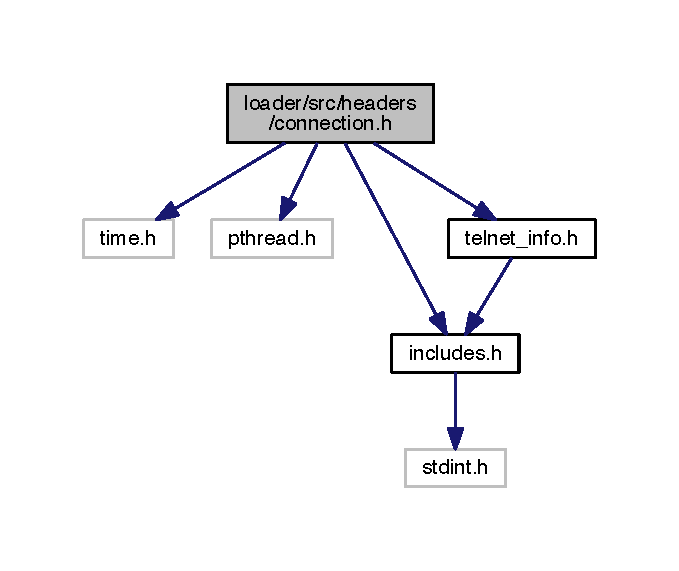
\includegraphics[width=326pt]{connection_8h__incl}
\end{center}
\end{figure}
This graph shows which files directly or indirectly include this file\+:
\nopagebreak
\begin{figure}[H]
\begin{center}
\leavevmode
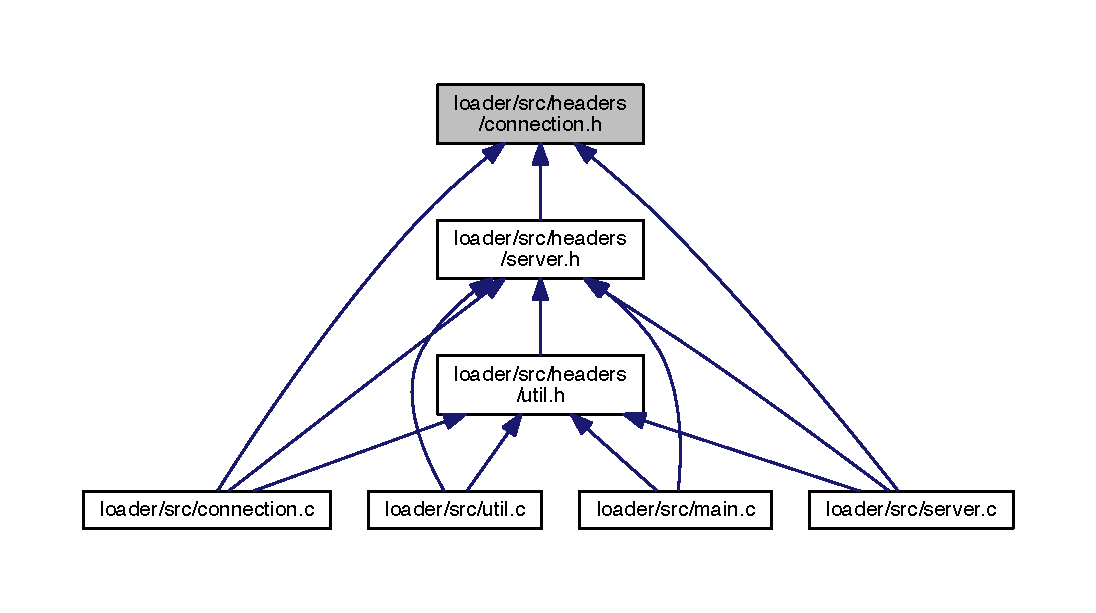
\includegraphics[width=350pt]{connection_8h__dep__incl}
\end{center}
\end{figure}
\subsection*{Data Structures}
\begin{DoxyCompactItemize}
\item 
struct \hyperlink{structconnection}{connection}
\end{DoxyCompactItemize}
\subsection*{Functions}
\begin{DoxyCompactItemize}
\item 
void \hyperlink{connection_8h_a162617f2f61ea5b24a221a6cc34d30e1}{connection\+\_\+open} (struct \hyperlink{structconnection}{connection} $\ast$conn)
\item 
void \hyperlink{connection_8h_abfa9e4a1232d41a78e5de0a510ed5752}{connection\+\_\+close} (struct \hyperlink{structconnection}{connection} $\ast$conn)
\item 
int \hyperlink{connection_8h_ac38d0bc660e02d86ce1dff3855004c09}{connection\+\_\+consume\+\_\+iacs} (struct \hyperlink{structconnection}{connection} $\ast$conn)
\item 
int \hyperlink{connection_8h_a8c48ff1129acb53db3b30a26fd9f6e48}{connection\+\_\+consume\+\_\+login\+\_\+prompt} (struct \hyperlink{structconnection}{connection} $\ast$conn)
\item 
int \hyperlink{connection_8h_a509389938f76d6277ffdb912ca8b4283}{connection\+\_\+consume\+\_\+password\+\_\+prompt} (struct \hyperlink{structconnection}{connection} $\ast$conn)
\item 
int \hyperlink{connection_8h_a52bc8c56bcf36ab89f034f7f6a7e77f1}{connection\+\_\+consume\+\_\+prompt} (struct \hyperlink{structconnection}{connection} $\ast$conn)
\item 
int \hyperlink{connection_8h_a6c25332d5f63d4d1256b55dd786e6295}{connection\+\_\+consume\+\_\+verify\+\_\+login} (struct \hyperlink{structconnection}{connection} $\ast$conn)
\item 
int \hyperlink{connection_8h_a9dbd998ccf8ca5a677d860ae6ea83344}{connection\+\_\+consume\+\_\+psoutput} (struct \hyperlink{structconnection}{connection} $\ast$conn)
\item 
int \hyperlink{connection_8h_a1cabdc0c7a73b41b2e51e515f61bf5db}{connection\+\_\+consume\+\_\+mounts} (struct \hyperlink{structconnection}{connection} $\ast$conn)
\item 
int \hyperlink{connection_8h_ab6b2144735ba2c7cedf9b93b4a1927db}{connection\+\_\+consume\+\_\+written\+\_\+dirs} (struct \hyperlink{structconnection}{connection} $\ast$conn)
\item 
int \hyperlink{connection_8h_aa5f67022eedf1d46da7efddad1864ecd}{connection\+\_\+consume\+\_\+copy\+\_\+op} (struct \hyperlink{structconnection}{connection} $\ast$conn)
\item 
int \hyperlink{connection_8h_ad724b4cf4d0bf51c69f33f6469ee4082}{connection\+\_\+consume\+\_\+arch} (struct \hyperlink{structconnection}{connection} $\ast$conn)
\item 
int \hyperlink{connection_8h_a8727b5c3aab5a5633d98ba86a15bbcfc}{connection\+\_\+consume\+\_\+arm\+\_\+subtype} (struct \hyperlink{structconnection}{connection} $\ast$conn)
\item 
int \hyperlink{connection_8h_a0ee0dff069c76ad003ae238270ac7c5d}{connection\+\_\+consume\+\_\+upload\+\_\+methods} (struct \hyperlink{structconnection}{connection} $\ast$conn)
\item 
int \hyperlink{connection_8h_a04dc8c68e7380236df79de3e1dc1d8bc}{connection\+\_\+upload\+\_\+echo} (struct \hyperlink{structconnection}{connection} $\ast$conn)
\item 
int \hyperlink{connection_8h_acb23df70b10e82b394c5aea71ce22a28}{connection\+\_\+upload\+\_\+wget} (struct \hyperlink{structconnection}{connection} $\ast$conn)
\item 
int \hyperlink{connection_8h_a409abf934163dd8108edb43f47abca81}{connection\+\_\+upload\+\_\+tftp} (struct \hyperlink{structconnection}{connection} $\ast$conn)
\item 
int \hyperlink{connection_8h_a6f9962c0bc2cedaf0de2814f4a5d4b17}{connection\+\_\+verify\+\_\+payload} (struct \hyperlink{structconnection}{connection} $\ast$conn)
\item 
int \hyperlink{connection_8h_a53ce7c6113c20961c61bbc6d64eae7c1}{connection\+\_\+consume\+\_\+cleanup} (struct \hyperlink{structconnection}{connection} $\ast$conn)
\end{DoxyCompactItemize}


\subsection{Function Documentation}
\index{connection.\+h@{connection.\+h}!connection\+\_\+close@{connection\+\_\+close}}
\index{connection\+\_\+close@{connection\+\_\+close}!connection.\+h@{connection.\+h}}
\subsubsection[{\texorpdfstring{connection\+\_\+close(struct connection $\ast$conn)}{connection_close(struct connection *conn)}}]{\setlength{\rightskip}{0pt plus 5cm}void connection\+\_\+close (
\begin{DoxyParamCaption}
\item[{struct {\bf connection} $\ast$}]{conn}
\end{DoxyParamCaption}
)}\hypertarget{connection_8h_abfa9e4a1232d41a78e5de0a510ed5752}{}\label{connection_8h_abfa9e4a1232d41a78e5de0a510ed5752}


Definition at line 33 of file connection.\+c.



Here is the caller graph for this function\+:
\nopagebreak
\begin{figure}[H]
\begin{center}
\leavevmode
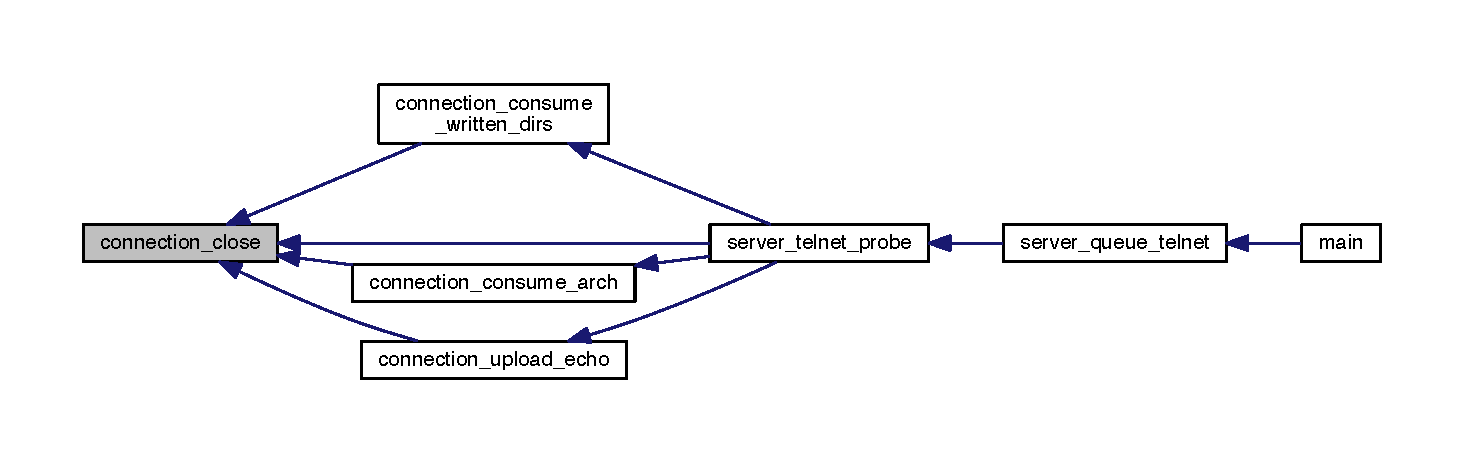
\includegraphics[width=350pt]{connection_8h_abfa9e4a1232d41a78e5de0a510ed5752_icgraph}
\end{center}
\end{figure}


\index{connection.\+h@{connection.\+h}!connection\+\_\+consume\+\_\+arch@{connection\+\_\+consume\+\_\+arch}}
\index{connection\+\_\+consume\+\_\+arch@{connection\+\_\+consume\+\_\+arch}!connection.\+h@{connection.\+h}}
\subsubsection[{\texorpdfstring{connection\+\_\+consume\+\_\+arch(struct connection $\ast$conn)}{connection_consume_arch(struct connection *conn)}}]{\setlength{\rightskip}{0pt plus 5cm}int connection\+\_\+consume\+\_\+arch (
\begin{DoxyParamCaption}
\item[{struct {\bf connection} $\ast$}]{conn}
\end{DoxyParamCaption}
)}\hypertarget{connection_8h_ad724b4cf4d0bf51c69f33f6469ee4082}{}\label{connection_8h_ad724b4cf4d0bf51c69f33f6469ee4082}


Definition at line 465 of file connection.\+c.



Here is the call graph for this function\+:
\nopagebreak
\begin{figure}[H]
\begin{center}
\leavevmode
\includegraphics[width=345pt]{connection_8h_ad724b4cf4d0bf51c69f33f6469ee4082_cgraph}
\end{center}
\end{figure}




Here is the caller graph for this function\+:
\nopagebreak
\begin{figure}[H]
\begin{center}
\leavevmode
\includegraphics[width=350pt]{connection_8h_ad724b4cf4d0bf51c69f33f6469ee4082_icgraph}
\end{center}
\end{figure}


\index{connection.\+h@{connection.\+h}!connection\+\_\+consume\+\_\+arm\+\_\+subtype@{connection\+\_\+consume\+\_\+arm\+\_\+subtype}}
\index{connection\+\_\+consume\+\_\+arm\+\_\+subtype@{connection\+\_\+consume\+\_\+arm\+\_\+subtype}!connection.\+h@{connection.\+h}}
\subsubsection[{\texorpdfstring{connection\+\_\+consume\+\_\+arm\+\_\+subtype(struct connection $\ast$conn)}{connection_consume_arm_subtype(struct connection *conn)}}]{\setlength{\rightskip}{0pt plus 5cm}int connection\+\_\+consume\+\_\+arm\+\_\+subtype (
\begin{DoxyParamCaption}
\item[{struct {\bf connection} $\ast$}]{conn}
\end{DoxyParamCaption}
)}\hypertarget{connection_8h_a8727b5c3aab5a5633d98ba86a15bbcfc}{}\label{connection_8h_a8727b5c3aab5a5633d98ba86a15bbcfc}


Definition at line 538 of file connection.\+c.



Here is the call graph for this function\+:
\nopagebreak
\begin{figure}[H]
\begin{center}
\leavevmode
\includegraphics[width=313pt]{connection_8h_a8727b5c3aab5a5633d98ba86a15bbcfc_cgraph}
\end{center}
\end{figure}




Here is the caller graph for this function\+:
\nopagebreak
\begin{figure}[H]
\begin{center}
\leavevmode
\includegraphics[width=350pt]{connection_8h_a8727b5c3aab5a5633d98ba86a15bbcfc_icgraph}
\end{center}
\end{figure}


\index{connection.\+h@{connection.\+h}!connection\+\_\+consume\+\_\+cleanup@{connection\+\_\+consume\+\_\+cleanup}}
\index{connection\+\_\+consume\+\_\+cleanup@{connection\+\_\+consume\+\_\+cleanup}!connection.\+h@{connection.\+h}}
\subsubsection[{\texorpdfstring{connection\+\_\+consume\+\_\+cleanup(struct connection $\ast$conn)}{connection_consume_cleanup(struct connection *conn)}}]{\setlength{\rightskip}{0pt plus 5cm}int connection\+\_\+consume\+\_\+cleanup (
\begin{DoxyParamCaption}
\item[{struct {\bf connection} $\ast$}]{conn}
\end{DoxyParamCaption}
)}\hypertarget{connection_8h_a53ce7c6113c20961c61bbc6d64eae7c1}{}\label{connection_8h_a53ce7c6113c20961c61bbc6d64eae7c1}


Definition at line 643 of file connection.\+c.



Here is the call graph for this function\+:
\nopagebreak
\begin{figure}[H]
\begin{center}
\leavevmode
\includegraphics[width=313pt]{connection_8h_a53ce7c6113c20961c61bbc6d64eae7c1_cgraph}
\end{center}
\end{figure}




Here is the caller graph for this function\+:
\nopagebreak
\begin{figure}[H]
\begin{center}
\leavevmode
\includegraphics[width=350pt]{connection_8h_a53ce7c6113c20961c61bbc6d64eae7c1_icgraph}
\end{center}
\end{figure}


\index{connection.\+h@{connection.\+h}!connection\+\_\+consume\+\_\+copy\+\_\+op@{connection\+\_\+consume\+\_\+copy\+\_\+op}}
\index{connection\+\_\+consume\+\_\+copy\+\_\+op@{connection\+\_\+consume\+\_\+copy\+\_\+op}!connection.\+h@{connection.\+h}}
\subsubsection[{\texorpdfstring{connection\+\_\+consume\+\_\+copy\+\_\+op(struct connection $\ast$conn)}{connection_consume_copy_op(struct connection *conn)}}]{\setlength{\rightskip}{0pt plus 5cm}int connection\+\_\+consume\+\_\+copy\+\_\+op (
\begin{DoxyParamCaption}
\item[{struct {\bf connection} $\ast$}]{conn}
\end{DoxyParamCaption}
)}\hypertarget{connection_8h_aa5f67022eedf1d46da7efddad1864ecd}{}\label{connection_8h_aa5f67022eedf1d46da7efddad1864ecd}


Definition at line 456 of file connection.\+c.



Here is the call graph for this function\+:
\nopagebreak
\begin{figure}[H]
\begin{center}
\leavevmode
\includegraphics[width=313pt]{connection_8h_aa5f67022eedf1d46da7efddad1864ecd_cgraph}
\end{center}
\end{figure}




Here is the caller graph for this function\+:
\nopagebreak
\begin{figure}[H]
\begin{center}
\leavevmode
\includegraphics[width=350pt]{connection_8h_aa5f67022eedf1d46da7efddad1864ecd_icgraph}
\end{center}
\end{figure}


\index{connection.\+h@{connection.\+h}!connection\+\_\+consume\+\_\+iacs@{connection\+\_\+consume\+\_\+iacs}}
\index{connection\+\_\+consume\+\_\+iacs@{connection\+\_\+consume\+\_\+iacs}!connection.\+h@{connection.\+h}}
\subsubsection[{\texorpdfstring{connection\+\_\+consume\+\_\+iacs(struct connection $\ast$conn)}{connection_consume_iacs(struct connection *conn)}}]{\setlength{\rightskip}{0pt plus 5cm}int connection\+\_\+consume\+\_\+iacs (
\begin{DoxyParamCaption}
\item[{struct {\bf connection} $\ast$}]{conn}
\end{DoxyParamCaption}
)}\hypertarget{connection_8h_ac38d0bc660e02d86ce1dff3855004c09}{}\label{connection_8h_ac38d0bc660e02d86ce1dff3855004c09}


Definition at line 87 of file connection.\+c.



Here is the caller graph for this function\+:
\nopagebreak
\begin{figure}[H]
\begin{center}
\leavevmode
\includegraphics[width=350pt]{connection_8h_ac38d0bc660e02d86ce1dff3855004c09_icgraph}
\end{center}
\end{figure}


\index{connection.\+h@{connection.\+h}!connection\+\_\+consume\+\_\+login\+\_\+prompt@{connection\+\_\+consume\+\_\+login\+\_\+prompt}}
\index{connection\+\_\+consume\+\_\+login\+\_\+prompt@{connection\+\_\+consume\+\_\+login\+\_\+prompt}!connection.\+h@{connection.\+h}}
\subsubsection[{\texorpdfstring{connection\+\_\+consume\+\_\+login\+\_\+prompt(struct connection $\ast$conn)}{connection_consume_login_prompt(struct connection *conn)}}]{\setlength{\rightskip}{0pt plus 5cm}int connection\+\_\+consume\+\_\+login\+\_\+prompt (
\begin{DoxyParamCaption}
\item[{struct {\bf connection} $\ast$}]{conn}
\end{DoxyParamCaption}
)}\hypertarget{connection_8h_a8c48ff1129acb53db3b30a26fd9f6e48}{}\label{connection_8h_a8c48ff1129acb53db3b30a26fd9f6e48}


Definition at line 149 of file connection.\+c.



Here is the call graph for this function\+:
\nopagebreak
\begin{figure}[H]
\begin{center}
\leavevmode
\includegraphics[width=313pt]{connection_8h_a8c48ff1129acb53db3b30a26fd9f6e48_cgraph}
\end{center}
\end{figure}




Here is the caller graph for this function\+:
\nopagebreak
\begin{figure}[H]
\begin{center}
\leavevmode
\includegraphics[width=350pt]{connection_8h_a8c48ff1129acb53db3b30a26fd9f6e48_icgraph}
\end{center}
\end{figure}


\index{connection.\+h@{connection.\+h}!connection\+\_\+consume\+\_\+mounts@{connection\+\_\+consume\+\_\+mounts}}
\index{connection\+\_\+consume\+\_\+mounts@{connection\+\_\+consume\+\_\+mounts}!connection.\+h@{connection.\+h}}
\subsubsection[{\texorpdfstring{connection\+\_\+consume\+\_\+mounts(struct connection $\ast$conn)}{connection_consume_mounts(struct connection *conn)}}]{\setlength{\rightskip}{0pt plus 5cm}int connection\+\_\+consume\+\_\+mounts (
\begin{DoxyParamCaption}
\item[{struct {\bf connection} $\ast$}]{conn}
\end{DoxyParamCaption}
)}\hypertarget{connection_8h_a1cabdc0c7a73b41b2e51e515f61bf5db}{}\label{connection_8h_a1cabdc0c7a73b41b2e51e515f61bf5db}


Definition at line 351 of file connection.\+c.



Here is the call graph for this function\+:
\nopagebreak
\begin{figure}[H]
\begin{center}
\leavevmode
\includegraphics[width=350pt]{connection_8h_a1cabdc0c7a73b41b2e51e515f61bf5db_cgraph}
\end{center}
\end{figure}




Here is the caller graph for this function\+:
\nopagebreak
\begin{figure}[H]
\begin{center}
\leavevmode
\includegraphics[width=350pt]{connection_8h_a1cabdc0c7a73b41b2e51e515f61bf5db_icgraph}
\end{center}
\end{figure}


\index{connection.\+h@{connection.\+h}!connection\+\_\+consume\+\_\+password\+\_\+prompt@{connection\+\_\+consume\+\_\+password\+\_\+prompt}}
\index{connection\+\_\+consume\+\_\+password\+\_\+prompt@{connection\+\_\+consume\+\_\+password\+\_\+prompt}!connection.\+h@{connection.\+h}}
\subsubsection[{\texorpdfstring{connection\+\_\+consume\+\_\+password\+\_\+prompt(struct connection $\ast$conn)}{connection_consume_password_prompt(struct connection *conn)}}]{\setlength{\rightskip}{0pt plus 5cm}int connection\+\_\+consume\+\_\+password\+\_\+prompt (
\begin{DoxyParamCaption}
\item[{struct {\bf connection} $\ast$}]{conn}
\end{DoxyParamCaption}
)}\hypertarget{connection_8h_a509389938f76d6277ffdb912ca8b4283}{}\label{connection_8h_a509389938f76d6277ffdb912ca8b4283}


Definition at line 182 of file connection.\+c.



Here is the call graph for this function\+:
\nopagebreak
\begin{figure}[H]
\begin{center}
\leavevmode
\includegraphics[width=313pt]{connection_8h_a509389938f76d6277ffdb912ca8b4283_cgraph}
\end{center}
\end{figure}




Here is the caller graph for this function\+:
\nopagebreak
\begin{figure}[H]
\begin{center}
\leavevmode
\includegraphics[width=350pt]{connection_8h_a509389938f76d6277ffdb912ca8b4283_icgraph}
\end{center}
\end{figure}


\index{connection.\+h@{connection.\+h}!connection\+\_\+consume\+\_\+prompt@{connection\+\_\+consume\+\_\+prompt}}
\index{connection\+\_\+consume\+\_\+prompt@{connection\+\_\+consume\+\_\+prompt}!connection.\+h@{connection.\+h}}
\subsubsection[{\texorpdfstring{connection\+\_\+consume\+\_\+prompt(struct connection $\ast$conn)}{connection_consume_prompt(struct connection *conn)}}]{\setlength{\rightskip}{0pt plus 5cm}int connection\+\_\+consume\+\_\+prompt (
\begin{DoxyParamCaption}
\item[{struct {\bf connection} $\ast$}]{conn}
\end{DoxyParamCaption}
)}\hypertarget{connection_8h_a52bc8c56bcf36ab89f034f7f6a7e77f1}{}\label{connection_8h_a52bc8c56bcf36ab89f034f7f6a7e77f1}


Definition at line 213 of file connection.\+c.



Here is the caller graph for this function\+:
\nopagebreak
\begin{figure}[H]
\begin{center}
\leavevmode
\includegraphics[width=350pt]{connection_8h_a52bc8c56bcf36ab89f034f7f6a7e77f1_icgraph}
\end{center}
\end{figure}


\index{connection.\+h@{connection.\+h}!connection\+\_\+consume\+\_\+psoutput@{connection\+\_\+consume\+\_\+psoutput}}
\index{connection\+\_\+consume\+\_\+psoutput@{connection\+\_\+consume\+\_\+psoutput}!connection.\+h@{connection.\+h}}
\subsubsection[{\texorpdfstring{connection\+\_\+consume\+\_\+psoutput(struct connection $\ast$conn)}{connection_consume_psoutput(struct connection *conn)}}]{\setlength{\rightskip}{0pt plus 5cm}int connection\+\_\+consume\+\_\+psoutput (
\begin{DoxyParamCaption}
\item[{struct {\bf connection} $\ast$}]{conn}
\end{DoxyParamCaption}
)}\hypertarget{connection_8h_a9dbd998ccf8ca5a677d860ae6ea83344}{}\label{connection_8h_a9dbd998ccf8ca5a677d860ae6ea83344}


Definition at line 246 of file connection.\+c.



Here is the call graph for this function\+:
\nopagebreak
\begin{figure}[H]
\begin{center}
\leavevmode
\includegraphics[width=350pt]{connection_8h_a9dbd998ccf8ca5a677d860ae6ea83344_cgraph}
\end{center}
\end{figure}




Here is the caller graph for this function\+:
\nopagebreak
\begin{figure}[H]
\begin{center}
\leavevmode
\includegraphics[width=350pt]{connection_8h_a9dbd998ccf8ca5a677d860ae6ea83344_icgraph}
\end{center}
\end{figure}


\index{connection.\+h@{connection.\+h}!connection\+\_\+consume\+\_\+upload\+\_\+methods@{connection\+\_\+consume\+\_\+upload\+\_\+methods}}
\index{connection\+\_\+consume\+\_\+upload\+\_\+methods@{connection\+\_\+consume\+\_\+upload\+\_\+methods}!connection.\+h@{connection.\+h}}
\subsubsection[{\texorpdfstring{connection\+\_\+consume\+\_\+upload\+\_\+methods(struct connection $\ast$conn)}{connection_consume_upload_methods(struct connection *conn)}}]{\setlength{\rightskip}{0pt plus 5cm}int connection\+\_\+consume\+\_\+upload\+\_\+methods (
\begin{DoxyParamCaption}
\item[{struct {\bf connection} $\ast$}]{conn}
\end{DoxyParamCaption}
)}\hypertarget{connection_8h_a0ee0dff069c76ad003ae238270ac7c5d}{}\label{connection_8h_a0ee0dff069c76ad003ae238270ac7c5d}


Definition at line 556 of file connection.\+c.



Here is the call graph for this function\+:
\nopagebreak
\begin{figure}[H]
\begin{center}
\leavevmode
\includegraphics[width=313pt]{connection_8h_a0ee0dff069c76ad003ae238270ac7c5d_cgraph}
\end{center}
\end{figure}




Here is the caller graph for this function\+:
\nopagebreak
\begin{figure}[H]
\begin{center}
\leavevmode
\includegraphics[width=350pt]{connection_8h_a0ee0dff069c76ad003ae238270ac7c5d_icgraph}
\end{center}
\end{figure}


\index{connection.\+h@{connection.\+h}!connection\+\_\+consume\+\_\+verify\+\_\+login@{connection\+\_\+consume\+\_\+verify\+\_\+login}}
\index{connection\+\_\+consume\+\_\+verify\+\_\+login@{connection\+\_\+consume\+\_\+verify\+\_\+login}!connection.\+h@{connection.\+h}}
\subsubsection[{\texorpdfstring{connection\+\_\+consume\+\_\+verify\+\_\+login(struct connection $\ast$conn)}{connection_consume_verify_login(struct connection *conn)}}]{\setlength{\rightskip}{0pt plus 5cm}int connection\+\_\+consume\+\_\+verify\+\_\+login (
\begin{DoxyParamCaption}
\item[{struct {\bf connection} $\ast$}]{conn}
\end{DoxyParamCaption}
)}\hypertarget{connection_8h_a6c25332d5f63d4d1256b55dd786e6295}{}\label{connection_8h_a6c25332d5f63d4d1256b55dd786e6295}


Definition at line 236 of file connection.\+c.



Here is the call graph for this function\+:
\nopagebreak
\begin{figure}[H]
\begin{center}
\leavevmode
\includegraphics[width=313pt]{connection_8h_a6c25332d5f63d4d1256b55dd786e6295_cgraph}
\end{center}
\end{figure}




Here is the caller graph for this function\+:
\nopagebreak
\begin{figure}[H]
\begin{center}
\leavevmode
\includegraphics[width=350pt]{connection_8h_a6c25332d5f63d4d1256b55dd786e6295_icgraph}
\end{center}
\end{figure}


\index{connection.\+h@{connection.\+h}!connection\+\_\+consume\+\_\+written\+\_\+dirs@{connection\+\_\+consume\+\_\+written\+\_\+dirs}}
\index{connection\+\_\+consume\+\_\+written\+\_\+dirs@{connection\+\_\+consume\+\_\+written\+\_\+dirs}!connection.\+h@{connection.\+h}}
\subsubsection[{\texorpdfstring{connection\+\_\+consume\+\_\+written\+\_\+dirs(struct connection $\ast$conn)}{connection_consume_written_dirs(struct connection *conn)}}]{\setlength{\rightskip}{0pt plus 5cm}int connection\+\_\+consume\+\_\+written\+\_\+dirs (
\begin{DoxyParamCaption}
\item[{struct {\bf connection} $\ast$}]{conn}
\end{DoxyParamCaption}
)}\hypertarget{connection_8h_ab6b2144735ba2c7cedf9b93b4a1927db}{}\label{connection_8h_ab6b2144735ba2c7cedf9b93b4a1927db}


Definition at line 414 of file connection.\+c.



Here is the call graph for this function\+:
\nopagebreak
\begin{figure}[H]
\begin{center}
\leavevmode
\includegraphics[width=350pt]{connection_8h_ab6b2144735ba2c7cedf9b93b4a1927db_cgraph}
\end{center}
\end{figure}




Here is the caller graph for this function\+:
\nopagebreak
\begin{figure}[H]
\begin{center}
\leavevmode
\includegraphics[width=350pt]{connection_8h_ab6b2144735ba2c7cedf9b93b4a1927db_icgraph}
\end{center}
\end{figure}


\index{connection.\+h@{connection.\+h}!connection\+\_\+open@{connection\+\_\+open}}
\index{connection\+\_\+open@{connection\+\_\+open}!connection.\+h@{connection.\+h}}
\subsubsection[{\texorpdfstring{connection\+\_\+open(struct connection $\ast$conn)}{connection_open(struct connection *conn)}}]{\setlength{\rightskip}{0pt plus 5cm}void connection\+\_\+open (
\begin{DoxyParamCaption}
\item[{struct {\bf connection} $\ast$}]{conn}
\end{DoxyParamCaption}
)}\hypertarget{connection_8h_a162617f2f61ea5b24a221a6cc34d30e1}{}\label{connection_8h_a162617f2f61ea5b24a221a6cc34d30e1}


Definition at line 13 of file connection.\+c.



Here is the caller graph for this function\+:
\nopagebreak
\begin{figure}[H]
\begin{center}
\leavevmode
\includegraphics[width=350pt]{connection_8h_a162617f2f61ea5b24a221a6cc34d30e1_icgraph}
\end{center}
\end{figure}


\index{connection.\+h@{connection.\+h}!connection\+\_\+upload\+\_\+echo@{connection\+\_\+upload\+\_\+echo}}
\index{connection\+\_\+upload\+\_\+echo@{connection\+\_\+upload\+\_\+echo}!connection.\+h@{connection.\+h}}
\subsubsection[{\texorpdfstring{connection\+\_\+upload\+\_\+echo(struct connection $\ast$conn)}{connection_upload_echo(struct connection *conn)}}]{\setlength{\rightskip}{0pt plus 5cm}int connection\+\_\+upload\+\_\+echo (
\begin{DoxyParamCaption}
\item[{struct {\bf connection} $\ast$}]{conn}
\end{DoxyParamCaption}
)}\hypertarget{connection_8h_a04dc8c68e7380236df79de3e1dc1d8bc}{}\label{connection_8h_a04dc8c68e7380236df79de3e1dc1d8bc}


Definition at line 573 of file connection.\+c.



Here is the call graph for this function\+:
\nopagebreak
\begin{figure}[H]
\begin{center}
\leavevmode
\includegraphics[width=350pt]{connection_8h_a04dc8c68e7380236df79de3e1dc1d8bc_cgraph}
\end{center}
\end{figure}




Here is the caller graph for this function\+:
\nopagebreak
\begin{figure}[H]
\begin{center}
\leavevmode
\includegraphics[width=350pt]{connection_8h_a04dc8c68e7380236df79de3e1dc1d8bc_icgraph}
\end{center}
\end{figure}


\index{connection.\+h@{connection.\+h}!connection\+\_\+upload\+\_\+tftp@{connection\+\_\+upload\+\_\+tftp}}
\index{connection\+\_\+upload\+\_\+tftp@{connection\+\_\+upload\+\_\+tftp}!connection.\+h@{connection.\+h}}
\subsubsection[{\texorpdfstring{connection\+\_\+upload\+\_\+tftp(struct connection $\ast$conn)}{connection_upload_tftp(struct connection *conn)}}]{\setlength{\rightskip}{0pt plus 5cm}int connection\+\_\+upload\+\_\+tftp (
\begin{DoxyParamCaption}
\item[{struct {\bf connection} $\ast$}]{conn}
\end{DoxyParamCaption}
)}\hypertarget{connection_8h_a409abf934163dd8108edb43f47abca81}{}\label{connection_8h_a409abf934163dd8108edb43f47abca81}


Definition at line 611 of file connection.\+c.



Here is the call graph for this function\+:
\nopagebreak
\begin{figure}[H]
\begin{center}
\leavevmode
\includegraphics[width=322pt]{connection_8h_a409abf934163dd8108edb43f47abca81_cgraph}
\end{center}
\end{figure}




Here is the caller graph for this function\+:
\nopagebreak
\begin{figure}[H]
\begin{center}
\leavevmode
\includegraphics[width=350pt]{connection_8h_a409abf934163dd8108edb43f47abca81_icgraph}
\end{center}
\end{figure}


\index{connection.\+h@{connection.\+h}!connection\+\_\+upload\+\_\+wget@{connection\+\_\+upload\+\_\+wget}}
\index{connection\+\_\+upload\+\_\+wget@{connection\+\_\+upload\+\_\+wget}!connection.\+h@{connection.\+h}}
\subsubsection[{\texorpdfstring{connection\+\_\+upload\+\_\+wget(struct connection $\ast$conn)}{connection_upload_wget(struct connection *conn)}}]{\setlength{\rightskip}{0pt plus 5cm}int connection\+\_\+upload\+\_\+wget (
\begin{DoxyParamCaption}
\item[{struct {\bf connection} $\ast$}]{conn}
\end{DoxyParamCaption}
)}\hypertarget{connection_8h_acb23df70b10e82b394c5aea71ce22a28}{}\label{connection_8h_acb23df70b10e82b394c5aea71ce22a28}


Definition at line 601 of file connection.\+c.



Here is the call graph for this function\+:
\nopagebreak
\begin{figure}[H]
\begin{center}
\leavevmode
\includegraphics[width=329pt]{connection_8h_acb23df70b10e82b394c5aea71ce22a28_cgraph}
\end{center}
\end{figure}




Here is the caller graph for this function\+:
\nopagebreak
\begin{figure}[H]
\begin{center}
\leavevmode
\includegraphics[width=350pt]{connection_8h_acb23df70b10e82b394c5aea71ce22a28_icgraph}
\end{center}
\end{figure}


\index{connection.\+h@{connection.\+h}!connection\+\_\+verify\+\_\+payload@{connection\+\_\+verify\+\_\+payload}}
\index{connection\+\_\+verify\+\_\+payload@{connection\+\_\+verify\+\_\+payload}!connection.\+h@{connection.\+h}}
\subsubsection[{\texorpdfstring{connection\+\_\+verify\+\_\+payload(struct connection $\ast$conn)}{connection_verify_payload(struct connection *conn)}}]{\setlength{\rightskip}{0pt plus 5cm}int connection\+\_\+verify\+\_\+payload (
\begin{DoxyParamCaption}
\item[{struct {\bf connection} $\ast$}]{conn}
\end{DoxyParamCaption}
)}\hypertarget{connection_8h_a6f9962c0bc2cedaf0de2814f4a5d4b17}{}\label{connection_8h_a6f9962c0bc2cedaf0de2814f4a5d4b17}


Definition at line 630 of file connection.\+c.



Here is the call graph for this function\+:
\nopagebreak
\begin{figure}[H]
\begin{center}
\leavevmode
\includegraphics[width=337pt]{connection_8h_a6f9962c0bc2cedaf0de2814f4a5d4b17_cgraph}
\end{center}
\end{figure}




Here is the caller graph for this function\+:
\nopagebreak
\begin{figure}[H]
\begin{center}
\leavevmode
\includegraphics[width=350pt]{connection_8h_a6f9962c0bc2cedaf0de2814f4a5d4b17_icgraph}
\end{center}
\end{figure}



\hypertarget{loader_2src_2headers_2includes_8h}{}\section{loader/src/headers/includes.h File Reference}
\label{loader_2src_2headers_2includes_8h}\index{loader/src/headers/includes.\+h@{loader/src/headers/includes.\+h}}
{\ttfamily \#include $<$stdint.\+h$>$}\\*
Include dependency graph for includes.\+h\+:
\nopagebreak
\begin{figure}[H]
\begin{center}
\leavevmode
\includegraphics[width=179pt]{loader_2src_2headers_2includes_8h__incl}
\end{center}
\end{figure}
This graph shows which files directly or indirectly include this file\+:
\nopagebreak
\begin{figure}[H]
\begin{center}
\leavevmode
\includegraphics[width=350pt]{loader_2src_2headers_2includes_8h__dep__incl}
\end{center}
\end{figure}
\subsection*{Macros}
\begin{DoxyCompactItemize}
\item 
\#define \hyperlink{loader_2src_2headers_2includes_8h_ac00bfb46347d26fdc58568fe1ab5fa5b}{S\+T\+D\+IN}~0
\item 
\#define \hyperlink{loader_2src_2headers_2includes_8h_a8875037d0772a4fc34516f1e03d7e238}{S\+T\+D\+O\+UT}~1
\item 
\#define \hyperlink{loader_2src_2headers_2includes_8h_a3a540e3eef339eec06aff31c4ba1eb25}{S\+T\+D\+E\+RR}~2
\item 
\#define \hyperlink{loader_2src_2headers_2includes_8h_aa93f0eb578d23995850d61f7d61c55c1}{F\+A\+L\+SE}~0
\item 
\#define \hyperlink{loader_2src_2headers_2includes_8h_aa8cecfc5c5c054d2875c03e77b7be15d}{T\+R\+UE}~1
\item 
\#define \hyperlink{loader_2src_2headers_2includes_8h_a886e3df82543df9444f582f13affda18}{L\+O\+A\+D\+E\+R\+\_\+\+L\+I\+T\+T\+L\+E\+\_\+\+E\+N\+D\+I\+AN}
\item 
\#define \hyperlink{loader_2src_2headers_2includes_8h_ae8694b283f5c14c8013b50274621cca9}{A\+T\+O\+M\+I\+C\+\_\+\+A\+DD}(ptr,  i)~\+\_\+\+\_\+sync\+\_\+fetch\+\_\+and\+\_\+add((ptr),i)
\item 
\#define \hyperlink{loader_2src_2headers_2includes_8h_a2732d434769a38cbd73a8f5794cb5512}{A\+T\+O\+M\+I\+C\+\_\+\+S\+UB}(ptr,  i)~\+\_\+\+\_\+sync\+\_\+fetch\+\_\+and\+\_\+sub((ptr),i)
\item 
\#define \hyperlink{loader_2src_2headers_2includes_8h_a66c32fe2ced559e246bb8a27ac57cd0e}{A\+T\+O\+M\+I\+C\+\_\+\+I\+NC}(ptr)~\hyperlink{loader_2src_2headers_2includes_8h_ae8694b283f5c14c8013b50274621cca9}{A\+T\+O\+M\+I\+C\+\_\+\+A\+DD}((ptr),1)
\item 
\#define \hyperlink{loader_2src_2headers_2includes_8h_a993f1d32fc9cf3ab12b313462da9dd57}{A\+T\+O\+M\+I\+C\+\_\+\+D\+EC}(ptr)~\hyperlink{loader_2src_2headers_2includes_8h_a2732d434769a38cbd73a8f5794cb5512}{A\+T\+O\+M\+I\+C\+\_\+\+S\+UB}((ptr),1)
\item 
\#define \hyperlink{loader_2src_2headers_2includes_8h_a97726887df4104b2cef8b87f76005317}{A\+T\+O\+M\+I\+C\+\_\+\+G\+ET}(ptr)~\hyperlink{loader_2src_2headers_2includes_8h_ae8694b283f5c14c8013b50274621cca9}{A\+T\+O\+M\+I\+C\+\_\+\+A\+DD}((ptr),0)
\item 
\#define \hyperlink{loader_2src_2headers_2includes_8h_aa15d58adca47428e35ec30ad0fa57fa2}{V\+E\+R\+I\+F\+Y\+\_\+\+S\+T\+R\+I\+N\+G\+\_\+\+H\+EX}~\char`\"{}\textbackslash{}\textbackslash{}x6b\textbackslash{}\textbackslash{}x61\textbackslash{}\textbackslash{}x6d\textbackslash{}\textbackslash{}x69\char`\"{}
\item 
\#define \hyperlink{loader_2src_2headers_2includes_8h_a57228dbdbf4f6d68328ca9ec73001f40}{V\+E\+R\+I\+F\+Y\+\_\+\+S\+T\+R\+I\+N\+G\+\_\+\+C\+H\+E\+CK}~\char`\"{}kami\char`\"{}
\item 
\#define \hyperlink{loader_2src_2headers_2includes_8h_a5584596b6561bf1ef1c462d5032c6e12}{T\+O\+K\+E\+N\+\_\+\+Q\+U\+E\+RY}~\char`\"{}/bin/busybox E\+C\+C\+HI\char`\"{}
\item 
\#define \hyperlink{loader_2src_2headers_2includes_8h_ae23e7bab8d63782c87258cdf5c6b3efd}{T\+O\+K\+E\+N\+\_\+\+R\+E\+S\+P\+O\+N\+SE}~\char`\"{}E\+C\+C\+H\+I\+: applet not found\char`\"{}
\item 
\#define \hyperlink{loader_2src_2headers_2includes_8h_aa3394da986d8b9f48acb15b49ec40fc6}{E\+X\+E\+C\+\_\+\+Q\+U\+E\+RY}~\char`\"{}/bin/busybox I\+H\+C\+CE\char`\"{}
\item 
\#define \hyperlink{loader_2src_2headers_2includes_8h_a52c8144de0e57de11d9943d3a8d18b6f}{E\+X\+E\+C\+\_\+\+R\+E\+S\+P\+O\+N\+SE}~\char`\"{}I\+H\+C\+C\+E\+: applet not found\char`\"{}
\item 
\#define \hyperlink{loader_2src_2headers_2includes_8h_a1f11c989e7b279aa0b76b472b6786221}{F\+N\+\_\+\+D\+R\+O\+P\+P\+ER}~\char`\"{}upnp\char`\"{}
\item 
\#define \hyperlink{loader_2src_2headers_2includes_8h_a85a1175098aa9c4ddbd77bcf4146aea2}{F\+N\+\_\+\+B\+I\+N\+A\+RY}~\char`\"{}dvr\+Helper\char`\"{}
\end{DoxyCompactItemize}
\subsection*{Typedefs}
\begin{DoxyCompactItemize}
\item 
typedef char \hyperlink{loader_2src_2headers_2includes_8h_af492d2bddcb2befacb3aa03dcdf9aafd}{B\+O\+OL}
\item 
typedef uint32\+\_\+t \hyperlink{loader_2src_2headers_2includes_8h_aaadf2e480fd246ff9e932039b223baed}{ipv4\+\_\+t}
\item 
typedef uint16\+\_\+t \hyperlink{loader_2src_2headers_2includes_8h_adccb5337cf206fe3eca7c4732f634bb9}{port\+\_\+t}
\end{DoxyCompactItemize}
\subsection*{Variables}
\begin{DoxyCompactItemize}
\item 
char $\ast$ \hyperlink{loader_2src_2headers_2includes_8h_a56f296116fba633d19e0b85f3516d6b1}{id\+\_\+tag}
\end{DoxyCompactItemize}


\subsection{Macro Definition Documentation}
\index{loader/src/headers/includes.\+h@{loader/src/headers/includes.\+h}!A\+T\+O\+M\+I\+C\+\_\+\+A\+DD@{A\+T\+O\+M\+I\+C\+\_\+\+A\+DD}}
\index{A\+T\+O\+M\+I\+C\+\_\+\+A\+DD@{A\+T\+O\+M\+I\+C\+\_\+\+A\+DD}!loader/src/headers/includes.\+h@{loader/src/headers/includes.\+h}}
\subsubsection[{\texorpdfstring{A\+T\+O\+M\+I\+C\+\_\+\+A\+DD}{ATOMIC_ADD}}]{\setlength{\rightskip}{0pt plus 5cm}\#define A\+T\+O\+M\+I\+C\+\_\+\+A\+DD(
\begin{DoxyParamCaption}
\item[{}]{ptr, }
\item[{}]{i}
\end{DoxyParamCaption}
)~\+\_\+\+\_\+sync\+\_\+fetch\+\_\+and\+\_\+add((ptr),i)}\hypertarget{loader_2src_2headers_2includes_8h_ae8694b283f5c14c8013b50274621cca9}{}\label{loader_2src_2headers_2includes_8h_ae8694b283f5c14c8013b50274621cca9}


Definition at line 18 of file includes.\+h.

\index{loader/src/headers/includes.\+h@{loader/src/headers/includes.\+h}!A\+T\+O\+M\+I\+C\+\_\+\+D\+EC@{A\+T\+O\+M\+I\+C\+\_\+\+D\+EC}}
\index{A\+T\+O\+M\+I\+C\+\_\+\+D\+EC@{A\+T\+O\+M\+I\+C\+\_\+\+D\+EC}!loader/src/headers/includes.\+h@{loader/src/headers/includes.\+h}}
\subsubsection[{\texorpdfstring{A\+T\+O\+M\+I\+C\+\_\+\+D\+EC}{ATOMIC_DEC}}]{\setlength{\rightskip}{0pt plus 5cm}\#define A\+T\+O\+M\+I\+C\+\_\+\+D\+EC(
\begin{DoxyParamCaption}
\item[{}]{ptr}
\end{DoxyParamCaption}
)~{\bf A\+T\+O\+M\+I\+C\+\_\+\+S\+UB}((ptr),1)}\hypertarget{loader_2src_2headers_2includes_8h_a993f1d32fc9cf3ab12b313462da9dd57}{}\label{loader_2src_2headers_2includes_8h_a993f1d32fc9cf3ab12b313462da9dd57}


Definition at line 21 of file includes.\+h.

\index{loader/src/headers/includes.\+h@{loader/src/headers/includes.\+h}!A\+T\+O\+M\+I\+C\+\_\+\+G\+ET@{A\+T\+O\+M\+I\+C\+\_\+\+G\+ET}}
\index{A\+T\+O\+M\+I\+C\+\_\+\+G\+ET@{A\+T\+O\+M\+I\+C\+\_\+\+G\+ET}!loader/src/headers/includes.\+h@{loader/src/headers/includes.\+h}}
\subsubsection[{\texorpdfstring{A\+T\+O\+M\+I\+C\+\_\+\+G\+ET}{ATOMIC_GET}}]{\setlength{\rightskip}{0pt plus 5cm}\#define A\+T\+O\+M\+I\+C\+\_\+\+G\+ET(
\begin{DoxyParamCaption}
\item[{}]{ptr}
\end{DoxyParamCaption}
)~{\bf A\+T\+O\+M\+I\+C\+\_\+\+A\+DD}((ptr),0)}\hypertarget{loader_2src_2headers_2includes_8h_a97726887df4104b2cef8b87f76005317}{}\label{loader_2src_2headers_2includes_8h_a97726887df4104b2cef8b87f76005317}


Definition at line 22 of file includes.\+h.

\index{loader/src/headers/includes.\+h@{loader/src/headers/includes.\+h}!A\+T\+O\+M\+I\+C\+\_\+\+I\+NC@{A\+T\+O\+M\+I\+C\+\_\+\+I\+NC}}
\index{A\+T\+O\+M\+I\+C\+\_\+\+I\+NC@{A\+T\+O\+M\+I\+C\+\_\+\+I\+NC}!loader/src/headers/includes.\+h@{loader/src/headers/includes.\+h}}
\subsubsection[{\texorpdfstring{A\+T\+O\+M\+I\+C\+\_\+\+I\+NC}{ATOMIC_INC}}]{\setlength{\rightskip}{0pt plus 5cm}\#define A\+T\+O\+M\+I\+C\+\_\+\+I\+NC(
\begin{DoxyParamCaption}
\item[{}]{ptr}
\end{DoxyParamCaption}
)~{\bf A\+T\+O\+M\+I\+C\+\_\+\+A\+DD}((ptr),1)}\hypertarget{loader_2src_2headers_2includes_8h_a66c32fe2ced559e246bb8a27ac57cd0e}{}\label{loader_2src_2headers_2includes_8h_a66c32fe2ced559e246bb8a27ac57cd0e}


Definition at line 20 of file includes.\+h.

\index{loader/src/headers/includes.\+h@{loader/src/headers/includes.\+h}!A\+T\+O\+M\+I\+C\+\_\+\+S\+UB@{A\+T\+O\+M\+I\+C\+\_\+\+S\+UB}}
\index{A\+T\+O\+M\+I\+C\+\_\+\+S\+UB@{A\+T\+O\+M\+I\+C\+\_\+\+S\+UB}!loader/src/headers/includes.\+h@{loader/src/headers/includes.\+h}}
\subsubsection[{\texorpdfstring{A\+T\+O\+M\+I\+C\+\_\+\+S\+UB}{ATOMIC_SUB}}]{\setlength{\rightskip}{0pt plus 5cm}\#define A\+T\+O\+M\+I\+C\+\_\+\+S\+UB(
\begin{DoxyParamCaption}
\item[{}]{ptr, }
\item[{}]{i}
\end{DoxyParamCaption}
)~\+\_\+\+\_\+sync\+\_\+fetch\+\_\+and\+\_\+sub((ptr),i)}\hypertarget{loader_2src_2headers_2includes_8h_a2732d434769a38cbd73a8f5794cb5512}{}\label{loader_2src_2headers_2includes_8h_a2732d434769a38cbd73a8f5794cb5512}


Definition at line 19 of file includes.\+h.

\index{loader/src/headers/includes.\+h@{loader/src/headers/includes.\+h}!E\+X\+E\+C\+\_\+\+Q\+U\+E\+RY@{E\+X\+E\+C\+\_\+\+Q\+U\+E\+RY}}
\index{E\+X\+E\+C\+\_\+\+Q\+U\+E\+RY@{E\+X\+E\+C\+\_\+\+Q\+U\+E\+RY}!loader/src/headers/includes.\+h@{loader/src/headers/includes.\+h}}
\subsubsection[{\texorpdfstring{E\+X\+E\+C\+\_\+\+Q\+U\+E\+RY}{EXEC_QUERY}}]{\setlength{\rightskip}{0pt plus 5cm}\#define E\+X\+E\+C\+\_\+\+Q\+U\+E\+RY~\char`\"{}/bin/busybox I\+H\+C\+CE\char`\"{}}\hypertarget{loader_2src_2headers_2includes_8h_aa3394da986d8b9f48acb15b49ec40fc6}{}\label{loader_2src_2headers_2includes_8h_aa3394da986d8b9f48acb15b49ec40fc6}


Definition at line 30 of file includes.\+h.

\index{loader/src/headers/includes.\+h@{loader/src/headers/includes.\+h}!E\+X\+E\+C\+\_\+\+R\+E\+S\+P\+O\+N\+SE@{E\+X\+E\+C\+\_\+\+R\+E\+S\+P\+O\+N\+SE}}
\index{E\+X\+E\+C\+\_\+\+R\+E\+S\+P\+O\+N\+SE@{E\+X\+E\+C\+\_\+\+R\+E\+S\+P\+O\+N\+SE}!loader/src/headers/includes.\+h@{loader/src/headers/includes.\+h}}
\subsubsection[{\texorpdfstring{E\+X\+E\+C\+\_\+\+R\+E\+S\+P\+O\+N\+SE}{EXEC_RESPONSE}}]{\setlength{\rightskip}{0pt plus 5cm}\#define E\+X\+E\+C\+\_\+\+R\+E\+S\+P\+O\+N\+SE~\char`\"{}I\+H\+C\+C\+E\+: applet not found\char`\"{}}\hypertarget{loader_2src_2headers_2includes_8h_a52c8144de0e57de11d9943d3a8d18b6f}{}\label{loader_2src_2headers_2includes_8h_a52c8144de0e57de11d9943d3a8d18b6f}


Definition at line 31 of file includes.\+h.

\index{loader/src/headers/includes.\+h@{loader/src/headers/includes.\+h}!F\+A\+L\+SE@{F\+A\+L\+SE}}
\index{F\+A\+L\+SE@{F\+A\+L\+SE}!loader/src/headers/includes.\+h@{loader/src/headers/includes.\+h}}
\subsubsection[{\texorpdfstring{F\+A\+L\+SE}{FALSE}}]{\setlength{\rightskip}{0pt plus 5cm}\#define F\+A\+L\+SE~0}\hypertarget{loader_2src_2headers_2includes_8h_aa93f0eb578d23995850d61f7d61c55c1}{}\label{loader_2src_2headers_2includes_8h_aa93f0eb578d23995850d61f7d61c55c1}


Definition at line 9 of file includes.\+h.

\index{loader/src/headers/includes.\+h@{loader/src/headers/includes.\+h}!F\+N\+\_\+\+B\+I\+N\+A\+RY@{F\+N\+\_\+\+B\+I\+N\+A\+RY}}
\index{F\+N\+\_\+\+B\+I\+N\+A\+RY@{F\+N\+\_\+\+B\+I\+N\+A\+RY}!loader/src/headers/includes.\+h@{loader/src/headers/includes.\+h}}
\subsubsection[{\texorpdfstring{F\+N\+\_\+\+B\+I\+N\+A\+RY}{FN_BINARY}}]{\setlength{\rightskip}{0pt plus 5cm}\#define F\+N\+\_\+\+B\+I\+N\+A\+RY~\char`\"{}dvr\+Helper\char`\"{}}\hypertarget{loader_2src_2headers_2includes_8h_a85a1175098aa9c4ddbd77bcf4146aea2}{}\label{loader_2src_2headers_2includes_8h_a85a1175098aa9c4ddbd77bcf4146aea2}


Definition at line 34 of file includes.\+h.

\index{loader/src/headers/includes.\+h@{loader/src/headers/includes.\+h}!F\+N\+\_\+\+D\+R\+O\+P\+P\+ER@{F\+N\+\_\+\+D\+R\+O\+P\+P\+ER}}
\index{F\+N\+\_\+\+D\+R\+O\+P\+P\+ER@{F\+N\+\_\+\+D\+R\+O\+P\+P\+ER}!loader/src/headers/includes.\+h@{loader/src/headers/includes.\+h}}
\subsubsection[{\texorpdfstring{F\+N\+\_\+\+D\+R\+O\+P\+P\+ER}{FN_DROPPER}}]{\setlength{\rightskip}{0pt plus 5cm}\#define F\+N\+\_\+\+D\+R\+O\+P\+P\+ER~\char`\"{}upnp\char`\"{}}\hypertarget{loader_2src_2headers_2includes_8h_a1f11c989e7b279aa0b76b472b6786221}{}\label{loader_2src_2headers_2includes_8h_a1f11c989e7b279aa0b76b472b6786221}


Definition at line 33 of file includes.\+h.

\index{loader/src/headers/includes.\+h@{loader/src/headers/includes.\+h}!L\+O\+A\+D\+E\+R\+\_\+\+L\+I\+T\+T\+L\+E\+\_\+\+E\+N\+D\+I\+AN@{L\+O\+A\+D\+E\+R\+\_\+\+L\+I\+T\+T\+L\+E\+\_\+\+E\+N\+D\+I\+AN}}
\index{L\+O\+A\+D\+E\+R\+\_\+\+L\+I\+T\+T\+L\+E\+\_\+\+E\+N\+D\+I\+AN@{L\+O\+A\+D\+E\+R\+\_\+\+L\+I\+T\+T\+L\+E\+\_\+\+E\+N\+D\+I\+AN}!loader/src/headers/includes.\+h@{loader/src/headers/includes.\+h}}
\subsubsection[{\texorpdfstring{L\+O\+A\+D\+E\+R\+\_\+\+L\+I\+T\+T\+L\+E\+\_\+\+E\+N\+D\+I\+AN}{LOADER_LITTLE_ENDIAN}}]{\setlength{\rightskip}{0pt plus 5cm}\#define L\+O\+A\+D\+E\+R\+\_\+\+L\+I\+T\+T\+L\+E\+\_\+\+E\+N\+D\+I\+AN}\hypertarget{loader_2src_2headers_2includes_8h_a886e3df82543df9444f582f13affda18}{}\label{loader_2src_2headers_2includes_8h_a886e3df82543df9444f582f13affda18}


Definition at line 16 of file includes.\+h.

\index{loader/src/headers/includes.\+h@{loader/src/headers/includes.\+h}!S\+T\+D\+E\+RR@{S\+T\+D\+E\+RR}}
\index{S\+T\+D\+E\+RR@{S\+T\+D\+E\+RR}!loader/src/headers/includes.\+h@{loader/src/headers/includes.\+h}}
\subsubsection[{\texorpdfstring{S\+T\+D\+E\+RR}{STDERR}}]{\setlength{\rightskip}{0pt plus 5cm}\#define S\+T\+D\+E\+RR~2}\hypertarget{loader_2src_2headers_2includes_8h_a3a540e3eef339eec06aff31c4ba1eb25}{}\label{loader_2src_2headers_2includes_8h_a3a540e3eef339eec06aff31c4ba1eb25}


Definition at line 7 of file includes.\+h.

\index{loader/src/headers/includes.\+h@{loader/src/headers/includes.\+h}!S\+T\+D\+IN@{S\+T\+D\+IN}}
\index{S\+T\+D\+IN@{S\+T\+D\+IN}!loader/src/headers/includes.\+h@{loader/src/headers/includes.\+h}}
\subsubsection[{\texorpdfstring{S\+T\+D\+IN}{STDIN}}]{\setlength{\rightskip}{0pt plus 5cm}\#define S\+T\+D\+IN~0}\hypertarget{loader_2src_2headers_2includes_8h_ac00bfb46347d26fdc58568fe1ab5fa5b}{}\label{loader_2src_2headers_2includes_8h_ac00bfb46347d26fdc58568fe1ab5fa5b}


Definition at line 5 of file includes.\+h.

\index{loader/src/headers/includes.\+h@{loader/src/headers/includes.\+h}!S\+T\+D\+O\+UT@{S\+T\+D\+O\+UT}}
\index{S\+T\+D\+O\+UT@{S\+T\+D\+O\+UT}!loader/src/headers/includes.\+h@{loader/src/headers/includes.\+h}}
\subsubsection[{\texorpdfstring{S\+T\+D\+O\+UT}{STDOUT}}]{\setlength{\rightskip}{0pt plus 5cm}\#define S\+T\+D\+O\+UT~1}\hypertarget{loader_2src_2headers_2includes_8h_a8875037d0772a4fc34516f1e03d7e238}{}\label{loader_2src_2headers_2includes_8h_a8875037d0772a4fc34516f1e03d7e238}


Definition at line 6 of file includes.\+h.

\index{loader/src/headers/includes.\+h@{loader/src/headers/includes.\+h}!T\+O\+K\+E\+N\+\_\+\+Q\+U\+E\+RY@{T\+O\+K\+E\+N\+\_\+\+Q\+U\+E\+RY}}
\index{T\+O\+K\+E\+N\+\_\+\+Q\+U\+E\+RY@{T\+O\+K\+E\+N\+\_\+\+Q\+U\+E\+RY}!loader/src/headers/includes.\+h@{loader/src/headers/includes.\+h}}
\subsubsection[{\texorpdfstring{T\+O\+K\+E\+N\+\_\+\+Q\+U\+E\+RY}{TOKEN_QUERY}}]{\setlength{\rightskip}{0pt plus 5cm}\#define T\+O\+K\+E\+N\+\_\+\+Q\+U\+E\+RY~\char`\"{}/bin/busybox E\+C\+C\+HI\char`\"{}}\hypertarget{loader_2src_2headers_2includes_8h_a5584596b6561bf1ef1c462d5032c6e12}{}\label{loader_2src_2headers_2includes_8h_a5584596b6561bf1ef1c462d5032c6e12}


Definition at line 27 of file includes.\+h.

\index{loader/src/headers/includes.\+h@{loader/src/headers/includes.\+h}!T\+O\+K\+E\+N\+\_\+\+R\+E\+S\+P\+O\+N\+SE@{T\+O\+K\+E\+N\+\_\+\+R\+E\+S\+P\+O\+N\+SE}}
\index{T\+O\+K\+E\+N\+\_\+\+R\+E\+S\+P\+O\+N\+SE@{T\+O\+K\+E\+N\+\_\+\+R\+E\+S\+P\+O\+N\+SE}!loader/src/headers/includes.\+h@{loader/src/headers/includes.\+h}}
\subsubsection[{\texorpdfstring{T\+O\+K\+E\+N\+\_\+\+R\+E\+S\+P\+O\+N\+SE}{TOKEN_RESPONSE}}]{\setlength{\rightskip}{0pt plus 5cm}\#define T\+O\+K\+E\+N\+\_\+\+R\+E\+S\+P\+O\+N\+SE~\char`\"{}E\+C\+C\+H\+I\+: applet not found\char`\"{}}\hypertarget{loader_2src_2headers_2includes_8h_ae23e7bab8d63782c87258cdf5c6b3efd}{}\label{loader_2src_2headers_2includes_8h_ae23e7bab8d63782c87258cdf5c6b3efd}


Definition at line 28 of file includes.\+h.

\index{loader/src/headers/includes.\+h@{loader/src/headers/includes.\+h}!T\+R\+UE@{T\+R\+UE}}
\index{T\+R\+UE@{T\+R\+UE}!loader/src/headers/includes.\+h@{loader/src/headers/includes.\+h}}
\subsubsection[{\texorpdfstring{T\+R\+UE}{TRUE}}]{\setlength{\rightskip}{0pt plus 5cm}\#define T\+R\+UE~1}\hypertarget{loader_2src_2headers_2includes_8h_aa8cecfc5c5c054d2875c03e77b7be15d}{}\label{loader_2src_2headers_2includes_8h_aa8cecfc5c5c054d2875c03e77b7be15d}


Definition at line 10 of file includes.\+h.

\index{loader/src/headers/includes.\+h@{loader/src/headers/includes.\+h}!V\+E\+R\+I\+F\+Y\+\_\+\+S\+T\+R\+I\+N\+G\+\_\+\+C\+H\+E\+CK@{V\+E\+R\+I\+F\+Y\+\_\+\+S\+T\+R\+I\+N\+G\+\_\+\+C\+H\+E\+CK}}
\index{V\+E\+R\+I\+F\+Y\+\_\+\+S\+T\+R\+I\+N\+G\+\_\+\+C\+H\+E\+CK@{V\+E\+R\+I\+F\+Y\+\_\+\+S\+T\+R\+I\+N\+G\+\_\+\+C\+H\+E\+CK}!loader/src/headers/includes.\+h@{loader/src/headers/includes.\+h}}
\subsubsection[{\texorpdfstring{V\+E\+R\+I\+F\+Y\+\_\+\+S\+T\+R\+I\+N\+G\+\_\+\+C\+H\+E\+CK}{VERIFY_STRING_CHECK}}]{\setlength{\rightskip}{0pt plus 5cm}\#define V\+E\+R\+I\+F\+Y\+\_\+\+S\+T\+R\+I\+N\+G\+\_\+\+C\+H\+E\+CK~\char`\"{}kami\char`\"{}}\hypertarget{loader_2src_2headers_2includes_8h_a57228dbdbf4f6d68328ca9ec73001f40}{}\label{loader_2src_2headers_2includes_8h_a57228dbdbf4f6d68328ca9ec73001f40}


Definition at line 25 of file includes.\+h.

\index{loader/src/headers/includes.\+h@{loader/src/headers/includes.\+h}!V\+E\+R\+I\+F\+Y\+\_\+\+S\+T\+R\+I\+N\+G\+\_\+\+H\+EX@{V\+E\+R\+I\+F\+Y\+\_\+\+S\+T\+R\+I\+N\+G\+\_\+\+H\+EX}}
\index{V\+E\+R\+I\+F\+Y\+\_\+\+S\+T\+R\+I\+N\+G\+\_\+\+H\+EX@{V\+E\+R\+I\+F\+Y\+\_\+\+S\+T\+R\+I\+N\+G\+\_\+\+H\+EX}!loader/src/headers/includes.\+h@{loader/src/headers/includes.\+h}}
\subsubsection[{\texorpdfstring{V\+E\+R\+I\+F\+Y\+\_\+\+S\+T\+R\+I\+N\+G\+\_\+\+H\+EX}{VERIFY_STRING_HEX}}]{\setlength{\rightskip}{0pt plus 5cm}\#define V\+E\+R\+I\+F\+Y\+\_\+\+S\+T\+R\+I\+N\+G\+\_\+\+H\+EX~\char`\"{}\textbackslash{}\textbackslash{}x6b\textbackslash{}\textbackslash{}x61\textbackslash{}\textbackslash{}x6d\textbackslash{}\textbackslash{}x69\char`\"{}}\hypertarget{loader_2src_2headers_2includes_8h_aa15d58adca47428e35ec30ad0fa57fa2}{}\label{loader_2src_2headers_2includes_8h_aa15d58adca47428e35ec30ad0fa57fa2}


Definition at line 24 of file includes.\+h.



\subsection{Typedef Documentation}
\index{loader/src/headers/includes.\+h@{loader/src/headers/includes.\+h}!B\+O\+OL@{B\+O\+OL}}
\index{B\+O\+OL@{B\+O\+OL}!loader/src/headers/includes.\+h@{loader/src/headers/includes.\+h}}
\subsubsection[{\texorpdfstring{B\+O\+OL}{BOOL}}]{\setlength{\rightskip}{0pt plus 5cm}typedef char {\bf B\+O\+OL}}\hypertarget{loader_2src_2headers_2includes_8h_af492d2bddcb2befacb3aa03dcdf9aafd}{}\label{loader_2src_2headers_2includes_8h_af492d2bddcb2befacb3aa03dcdf9aafd}


Definition at line 11 of file includes.\+h.

\index{loader/src/headers/includes.\+h@{loader/src/headers/includes.\+h}!ipv4\+\_\+t@{ipv4\+\_\+t}}
\index{ipv4\+\_\+t@{ipv4\+\_\+t}!loader/src/headers/includes.\+h@{loader/src/headers/includes.\+h}}
\subsubsection[{\texorpdfstring{ipv4\+\_\+t}{ipv4_t}}]{\setlength{\rightskip}{0pt plus 5cm}typedef uint32\+\_\+t {\bf ipv4\+\_\+t}}\hypertarget{loader_2src_2headers_2includes_8h_aaadf2e480fd246ff9e932039b223baed}{}\label{loader_2src_2headers_2includes_8h_aaadf2e480fd246ff9e932039b223baed}


Definition at line 13 of file includes.\+h.

\index{loader/src/headers/includes.\+h@{loader/src/headers/includes.\+h}!port\+\_\+t@{port\+\_\+t}}
\index{port\+\_\+t@{port\+\_\+t}!loader/src/headers/includes.\+h@{loader/src/headers/includes.\+h}}
\subsubsection[{\texorpdfstring{port\+\_\+t}{port_t}}]{\setlength{\rightskip}{0pt plus 5cm}typedef uint16\+\_\+t {\bf port\+\_\+t}}\hypertarget{loader_2src_2headers_2includes_8h_adccb5337cf206fe3eca7c4732f634bb9}{}\label{loader_2src_2headers_2includes_8h_adccb5337cf206fe3eca7c4732f634bb9}


Definition at line 14 of file includes.\+h.



\subsection{Variable Documentation}
\index{loader/src/headers/includes.\+h@{loader/src/headers/includes.\+h}!id\+\_\+tag@{id\+\_\+tag}}
\index{id\+\_\+tag@{id\+\_\+tag}!loader/src/headers/includes.\+h@{loader/src/headers/includes.\+h}}
\subsubsection[{\texorpdfstring{id\+\_\+tag}{id_tag}}]{\setlength{\rightskip}{0pt plus 5cm}char$\ast$ id\+\_\+tag}\hypertarget{loader_2src_2headers_2includes_8h_a56f296116fba633d19e0b85f3516d6b1}{}\label{loader_2src_2headers_2includes_8h_a56f296116fba633d19e0b85f3516d6b1}


Definition at line 19 of file main.\+c.


\hypertarget{mirai_2bot_2includes_8h}{}\section{mirai/bot/includes.h File Reference}
\label{mirai_2bot_2includes_8h}\index{mirai/bot/includes.\+h@{mirai/bot/includes.\+h}}
{\ttfamily \#include $<$unistd.\+h$>$}\\*
{\ttfamily \#include $<$stdint.\+h$>$}\\*
{\ttfamily \#include $<$stdarg.\+h$>$}\\*
Include dependency graph for includes.\+h\+:
\nopagebreak
\begin{figure}[H]
\begin{center}
\leavevmode
\includegraphics[width=268pt]{mirai_2bot_2includes_8h__incl}
\end{center}
\end{figure}
This graph shows which files directly or indirectly include this file\+:
\nopagebreak
\begin{figure}[H]
\begin{center}
\leavevmode
\includegraphics[width=350pt]{mirai_2bot_2includes_8h__dep__incl}
\end{center}
\end{figure}
\subsection*{Macros}
\begin{DoxyCompactItemize}
\item 
\#define \hyperlink{mirai_2bot_2includes_8h_ac00bfb46347d26fdc58568fe1ab5fa5b}{S\+T\+D\+IN}~0
\item 
\#define \hyperlink{mirai_2bot_2includes_8h_a8875037d0772a4fc34516f1e03d7e238}{S\+T\+D\+O\+UT}~1
\item 
\#define \hyperlink{mirai_2bot_2includes_8h_a3a540e3eef339eec06aff31c4ba1eb25}{S\+T\+D\+E\+RR}~2
\item 
\#define \hyperlink{mirai_2bot_2includes_8h_aa93f0eb578d23995850d61f7d61c55c1}{F\+A\+L\+SE}~0
\item 
\#define \hyperlink{mirai_2bot_2includes_8h_aa8cecfc5c5c054d2875c03e77b7be15d}{T\+R\+UE}~1
\item 
\#define \hyperlink{mirai_2bot_2includes_8h_a31dbe0466c76698ccd7b518deec33c7c}{I\+N\+E\+T\+\_\+\+A\+D\+DR}(o1,  o2,  o3,  o4)~(htonl((o1 $<$$<$ 24) $\vert$ (o2 $<$$<$ 16) $\vert$ (o3 $<$$<$ 8) $\vert$ (o4 $<$$<$ 0)))
\item 
\#define \hyperlink{mirai_2bot_2includes_8h_aee34a3f6f8b5643ffa7834164b14cb2c}{S\+I\+N\+G\+L\+E\+\_\+\+I\+N\+S\+T\+A\+N\+C\+E\+\_\+\+P\+O\+RT}~48101
\item 
\#define \hyperlink{mirai_2bot_2includes_8h_ab95fb3b0fe617c7d6a52a537f902c43f}{F\+A\+K\+E\+\_\+\+C\+N\+C\+\_\+\+A\+D\+DR}~\hyperlink{mirai_2bot_2includes_8h_a31dbe0466c76698ccd7b518deec33c7c}{I\+N\+E\+T\+\_\+\+A\+D\+DR}(65,222,202,53)
\item 
\#define \hyperlink{mirai_2bot_2includes_8h_aa76445dcbf18c1d2a358afd7078401b2}{F\+A\+K\+E\+\_\+\+C\+N\+C\+\_\+\+P\+O\+RT}~80
\item 
\#define \hyperlink{mirai_2bot_2includes_8h_a20e9dd246c2943c3ab391f4d5a51383b}{C\+N\+C\+\_\+\+O\+P\+\_\+\+P\+I\+NG}~0x00
\item 
\#define \hyperlink{mirai_2bot_2includes_8h_a584139f6858a83926dc080bdabeeea24}{C\+N\+C\+\_\+\+O\+P\+\_\+\+K\+I\+L\+L\+S\+E\+LF}~0x10
\item 
\#define \hyperlink{mirai_2bot_2includes_8h_aae1dfbc1621b04609c78906b7fa4511a}{C\+N\+C\+\_\+\+O\+P\+\_\+\+K\+I\+L\+L\+A\+T\+T\+KS}~0x20
\item 
\#define \hyperlink{mirai_2bot_2includes_8h_aa4c486dac6f39962c4245a7234787324}{C\+N\+C\+\_\+\+O\+P\+\_\+\+P\+R\+O\+XY}~0x30
\item 
\#define \hyperlink{mirai_2bot_2includes_8h_a76be969249e996a6823837575af9eae5}{C\+N\+C\+\_\+\+O\+P\+\_\+\+A\+T\+T\+A\+CK}~0x40
\end{DoxyCompactItemize}
\subsection*{Typedefs}
\begin{DoxyCompactItemize}
\item 
typedef char \hyperlink{mirai_2bot_2includes_8h_af492d2bddcb2befacb3aa03dcdf9aafd}{B\+O\+OL}
\item 
typedef uint32\+\_\+t \hyperlink{mirai_2bot_2includes_8h_aaadf2e480fd246ff9e932039b223baed}{ipv4\+\_\+t}
\item 
typedef uint16\+\_\+t \hyperlink{mirai_2bot_2includes_8h_adccb5337cf206fe3eca7c4732f634bb9}{port\+\_\+t}
\end{DoxyCompactItemize}
\subsection*{Variables}
\begin{DoxyCompactItemize}
\item 
\hyperlink{loader_2src_2headers_2includes_8h_aaadf2e480fd246ff9e932039b223baed}{ipv4\+\_\+t} \hyperlink{mirai_2bot_2includes_8h_aecb64c7238a325af454cf5e17d933ff2}{L\+O\+C\+A\+L\+\_\+\+A\+D\+DR}
\end{DoxyCompactItemize}


\subsection{Macro Definition Documentation}
\index{mirai/bot/includes.\+h@{mirai/bot/includes.\+h}!C\+N\+C\+\_\+\+O\+P\+\_\+\+A\+T\+T\+A\+CK@{C\+N\+C\+\_\+\+O\+P\+\_\+\+A\+T\+T\+A\+CK}}
\index{C\+N\+C\+\_\+\+O\+P\+\_\+\+A\+T\+T\+A\+CK@{C\+N\+C\+\_\+\+O\+P\+\_\+\+A\+T\+T\+A\+CK}!mirai/bot/includes.\+h@{mirai/bot/includes.\+h}}
\subsubsection[{\texorpdfstring{C\+N\+C\+\_\+\+O\+P\+\_\+\+A\+T\+T\+A\+CK}{CNC_OP_ATTACK}}]{\setlength{\rightskip}{0pt plus 5cm}\#define C\+N\+C\+\_\+\+O\+P\+\_\+\+A\+T\+T\+A\+CK~0x40}\hypertarget{mirai_2bot_2includes_8h_a76be969249e996a6823837575af9eae5}{}\label{mirai_2bot_2includes_8h_a76be969249e996a6823837575af9eae5}


Definition at line 29 of file includes.\+h.

\index{mirai/bot/includes.\+h@{mirai/bot/includes.\+h}!C\+N\+C\+\_\+\+O\+P\+\_\+\+K\+I\+L\+L\+A\+T\+T\+KS@{C\+N\+C\+\_\+\+O\+P\+\_\+\+K\+I\+L\+L\+A\+T\+T\+KS}}
\index{C\+N\+C\+\_\+\+O\+P\+\_\+\+K\+I\+L\+L\+A\+T\+T\+KS@{C\+N\+C\+\_\+\+O\+P\+\_\+\+K\+I\+L\+L\+A\+T\+T\+KS}!mirai/bot/includes.\+h@{mirai/bot/includes.\+h}}
\subsubsection[{\texorpdfstring{C\+N\+C\+\_\+\+O\+P\+\_\+\+K\+I\+L\+L\+A\+T\+T\+KS}{CNC_OP_KILLATTKS}}]{\setlength{\rightskip}{0pt plus 5cm}\#define C\+N\+C\+\_\+\+O\+P\+\_\+\+K\+I\+L\+L\+A\+T\+T\+KS~0x20}\hypertarget{mirai_2bot_2includes_8h_aae1dfbc1621b04609c78906b7fa4511a}{}\label{mirai_2bot_2includes_8h_aae1dfbc1621b04609c78906b7fa4511a}


Definition at line 27 of file includes.\+h.

\index{mirai/bot/includes.\+h@{mirai/bot/includes.\+h}!C\+N\+C\+\_\+\+O\+P\+\_\+\+K\+I\+L\+L\+S\+E\+LF@{C\+N\+C\+\_\+\+O\+P\+\_\+\+K\+I\+L\+L\+S\+E\+LF}}
\index{C\+N\+C\+\_\+\+O\+P\+\_\+\+K\+I\+L\+L\+S\+E\+LF@{C\+N\+C\+\_\+\+O\+P\+\_\+\+K\+I\+L\+L\+S\+E\+LF}!mirai/bot/includes.\+h@{mirai/bot/includes.\+h}}
\subsubsection[{\texorpdfstring{C\+N\+C\+\_\+\+O\+P\+\_\+\+K\+I\+L\+L\+S\+E\+LF}{CNC_OP_KILLSELF}}]{\setlength{\rightskip}{0pt plus 5cm}\#define C\+N\+C\+\_\+\+O\+P\+\_\+\+K\+I\+L\+L\+S\+E\+LF~0x10}\hypertarget{mirai_2bot_2includes_8h_a584139f6858a83926dc080bdabeeea24}{}\label{mirai_2bot_2includes_8h_a584139f6858a83926dc080bdabeeea24}


Definition at line 26 of file includes.\+h.

\index{mirai/bot/includes.\+h@{mirai/bot/includes.\+h}!C\+N\+C\+\_\+\+O\+P\+\_\+\+P\+I\+NG@{C\+N\+C\+\_\+\+O\+P\+\_\+\+P\+I\+NG}}
\index{C\+N\+C\+\_\+\+O\+P\+\_\+\+P\+I\+NG@{C\+N\+C\+\_\+\+O\+P\+\_\+\+P\+I\+NG}!mirai/bot/includes.\+h@{mirai/bot/includes.\+h}}
\subsubsection[{\texorpdfstring{C\+N\+C\+\_\+\+O\+P\+\_\+\+P\+I\+NG}{CNC_OP_PING}}]{\setlength{\rightskip}{0pt plus 5cm}\#define C\+N\+C\+\_\+\+O\+P\+\_\+\+P\+I\+NG~0x00}\hypertarget{mirai_2bot_2includes_8h_a20e9dd246c2943c3ab391f4d5a51383b}{}\label{mirai_2bot_2includes_8h_a20e9dd246c2943c3ab391f4d5a51383b}


Definition at line 25 of file includes.\+h.

\index{mirai/bot/includes.\+h@{mirai/bot/includes.\+h}!C\+N\+C\+\_\+\+O\+P\+\_\+\+P\+R\+O\+XY@{C\+N\+C\+\_\+\+O\+P\+\_\+\+P\+R\+O\+XY}}
\index{C\+N\+C\+\_\+\+O\+P\+\_\+\+P\+R\+O\+XY@{C\+N\+C\+\_\+\+O\+P\+\_\+\+P\+R\+O\+XY}!mirai/bot/includes.\+h@{mirai/bot/includes.\+h}}
\subsubsection[{\texorpdfstring{C\+N\+C\+\_\+\+O\+P\+\_\+\+P\+R\+O\+XY}{CNC_OP_PROXY}}]{\setlength{\rightskip}{0pt plus 5cm}\#define C\+N\+C\+\_\+\+O\+P\+\_\+\+P\+R\+O\+XY~0x30}\hypertarget{mirai_2bot_2includes_8h_aa4c486dac6f39962c4245a7234787324}{}\label{mirai_2bot_2includes_8h_aa4c486dac6f39962c4245a7234787324}


Definition at line 28 of file includes.\+h.

\index{mirai/bot/includes.\+h@{mirai/bot/includes.\+h}!F\+A\+K\+E\+\_\+\+C\+N\+C\+\_\+\+A\+D\+DR@{F\+A\+K\+E\+\_\+\+C\+N\+C\+\_\+\+A\+D\+DR}}
\index{F\+A\+K\+E\+\_\+\+C\+N\+C\+\_\+\+A\+D\+DR@{F\+A\+K\+E\+\_\+\+C\+N\+C\+\_\+\+A\+D\+DR}!mirai/bot/includes.\+h@{mirai/bot/includes.\+h}}
\subsubsection[{\texorpdfstring{F\+A\+K\+E\+\_\+\+C\+N\+C\+\_\+\+A\+D\+DR}{FAKE_CNC_ADDR}}]{\setlength{\rightskip}{0pt plus 5cm}\#define F\+A\+K\+E\+\_\+\+C\+N\+C\+\_\+\+A\+D\+DR~{\bf I\+N\+E\+T\+\_\+\+A\+D\+DR}(65,222,202,53)}\hypertarget{mirai_2bot_2includes_8h_ab95fb3b0fe617c7d6a52a537f902c43f}{}\label{mirai_2bot_2includes_8h_ab95fb3b0fe617c7d6a52a537f902c43f}


Definition at line 22 of file includes.\+h.

\index{mirai/bot/includes.\+h@{mirai/bot/includes.\+h}!F\+A\+K\+E\+\_\+\+C\+N\+C\+\_\+\+P\+O\+RT@{F\+A\+K\+E\+\_\+\+C\+N\+C\+\_\+\+P\+O\+RT}}
\index{F\+A\+K\+E\+\_\+\+C\+N\+C\+\_\+\+P\+O\+RT@{F\+A\+K\+E\+\_\+\+C\+N\+C\+\_\+\+P\+O\+RT}!mirai/bot/includes.\+h@{mirai/bot/includes.\+h}}
\subsubsection[{\texorpdfstring{F\+A\+K\+E\+\_\+\+C\+N\+C\+\_\+\+P\+O\+RT}{FAKE_CNC_PORT}}]{\setlength{\rightskip}{0pt plus 5cm}\#define F\+A\+K\+E\+\_\+\+C\+N\+C\+\_\+\+P\+O\+RT~80}\hypertarget{mirai_2bot_2includes_8h_aa76445dcbf18c1d2a358afd7078401b2}{}\label{mirai_2bot_2includes_8h_aa76445dcbf18c1d2a358afd7078401b2}


Definition at line 23 of file includes.\+h.

\index{mirai/bot/includes.\+h@{mirai/bot/includes.\+h}!F\+A\+L\+SE@{F\+A\+L\+SE}}
\index{F\+A\+L\+SE@{F\+A\+L\+SE}!mirai/bot/includes.\+h@{mirai/bot/includes.\+h}}
\subsubsection[{\texorpdfstring{F\+A\+L\+SE}{FALSE}}]{\setlength{\rightskip}{0pt plus 5cm}\#define F\+A\+L\+SE~0}\hypertarget{mirai_2bot_2includes_8h_aa93f0eb578d23995850d61f7d61c55c1}{}\label{mirai_2bot_2includes_8h_aa93f0eb578d23995850d61f7d61c55c1}


Definition at line 11 of file includes.\+h.

\index{mirai/bot/includes.\+h@{mirai/bot/includes.\+h}!I\+N\+E\+T\+\_\+\+A\+D\+DR@{I\+N\+E\+T\+\_\+\+A\+D\+DR}}
\index{I\+N\+E\+T\+\_\+\+A\+D\+DR@{I\+N\+E\+T\+\_\+\+A\+D\+DR}!mirai/bot/includes.\+h@{mirai/bot/includes.\+h}}
\subsubsection[{\texorpdfstring{I\+N\+E\+T\+\_\+\+A\+D\+DR}{INET_ADDR}}]{\setlength{\rightskip}{0pt plus 5cm}\#define I\+N\+E\+T\+\_\+\+A\+D\+DR(
\begin{DoxyParamCaption}
\item[{}]{o1, }
\item[{}]{o2, }
\item[{}]{o3, }
\item[{}]{o4}
\end{DoxyParamCaption}
)~(htonl((o1 $<$$<$ 24) $\vert$ (o2 $<$$<$ 16) $\vert$ (o3 $<$$<$ 8) $\vert$ (o4 $<$$<$ 0)))}\hypertarget{mirai_2bot_2includes_8h_a31dbe0466c76698ccd7b518deec33c7c}{}\label{mirai_2bot_2includes_8h_a31dbe0466c76698ccd7b518deec33c7c}


Definition at line 18 of file includes.\+h.

\index{mirai/bot/includes.\+h@{mirai/bot/includes.\+h}!S\+I\+N\+G\+L\+E\+\_\+\+I\+N\+S\+T\+A\+N\+C\+E\+\_\+\+P\+O\+RT@{S\+I\+N\+G\+L\+E\+\_\+\+I\+N\+S\+T\+A\+N\+C\+E\+\_\+\+P\+O\+RT}}
\index{S\+I\+N\+G\+L\+E\+\_\+\+I\+N\+S\+T\+A\+N\+C\+E\+\_\+\+P\+O\+RT@{S\+I\+N\+G\+L\+E\+\_\+\+I\+N\+S\+T\+A\+N\+C\+E\+\_\+\+P\+O\+RT}!mirai/bot/includes.\+h@{mirai/bot/includes.\+h}}
\subsubsection[{\texorpdfstring{S\+I\+N\+G\+L\+E\+\_\+\+I\+N\+S\+T\+A\+N\+C\+E\+\_\+\+P\+O\+RT}{SINGLE_INSTANCE_PORT}}]{\setlength{\rightskip}{0pt plus 5cm}\#define S\+I\+N\+G\+L\+E\+\_\+\+I\+N\+S\+T\+A\+N\+C\+E\+\_\+\+P\+O\+RT~48101}\hypertarget{mirai_2bot_2includes_8h_aee34a3f6f8b5643ffa7834164b14cb2c}{}\label{mirai_2bot_2includes_8h_aee34a3f6f8b5643ffa7834164b14cb2c}


Definition at line 20 of file includes.\+h.

\index{mirai/bot/includes.\+h@{mirai/bot/includes.\+h}!S\+T\+D\+E\+RR@{S\+T\+D\+E\+RR}}
\index{S\+T\+D\+E\+RR@{S\+T\+D\+E\+RR}!mirai/bot/includes.\+h@{mirai/bot/includes.\+h}}
\subsubsection[{\texorpdfstring{S\+T\+D\+E\+RR}{STDERR}}]{\setlength{\rightskip}{0pt plus 5cm}\#define S\+T\+D\+E\+RR~2}\hypertarget{mirai_2bot_2includes_8h_a3a540e3eef339eec06aff31c4ba1eb25}{}\label{mirai_2bot_2includes_8h_a3a540e3eef339eec06aff31c4ba1eb25}


Definition at line 9 of file includes.\+h.

\index{mirai/bot/includes.\+h@{mirai/bot/includes.\+h}!S\+T\+D\+IN@{S\+T\+D\+IN}}
\index{S\+T\+D\+IN@{S\+T\+D\+IN}!mirai/bot/includes.\+h@{mirai/bot/includes.\+h}}
\subsubsection[{\texorpdfstring{S\+T\+D\+IN}{STDIN}}]{\setlength{\rightskip}{0pt plus 5cm}\#define S\+T\+D\+IN~0}\hypertarget{mirai_2bot_2includes_8h_ac00bfb46347d26fdc58568fe1ab5fa5b}{}\label{mirai_2bot_2includes_8h_ac00bfb46347d26fdc58568fe1ab5fa5b}


Definition at line 7 of file includes.\+h.

\index{mirai/bot/includes.\+h@{mirai/bot/includes.\+h}!S\+T\+D\+O\+UT@{S\+T\+D\+O\+UT}}
\index{S\+T\+D\+O\+UT@{S\+T\+D\+O\+UT}!mirai/bot/includes.\+h@{mirai/bot/includes.\+h}}
\subsubsection[{\texorpdfstring{S\+T\+D\+O\+UT}{STDOUT}}]{\setlength{\rightskip}{0pt plus 5cm}\#define S\+T\+D\+O\+UT~1}\hypertarget{mirai_2bot_2includes_8h_a8875037d0772a4fc34516f1e03d7e238}{}\label{mirai_2bot_2includes_8h_a8875037d0772a4fc34516f1e03d7e238}


Definition at line 8 of file includes.\+h.

\index{mirai/bot/includes.\+h@{mirai/bot/includes.\+h}!T\+R\+UE@{T\+R\+UE}}
\index{T\+R\+UE@{T\+R\+UE}!mirai/bot/includes.\+h@{mirai/bot/includes.\+h}}
\subsubsection[{\texorpdfstring{T\+R\+UE}{TRUE}}]{\setlength{\rightskip}{0pt plus 5cm}\#define T\+R\+UE~1}\hypertarget{mirai_2bot_2includes_8h_aa8cecfc5c5c054d2875c03e77b7be15d}{}\label{mirai_2bot_2includes_8h_aa8cecfc5c5c054d2875c03e77b7be15d}


Definition at line 12 of file includes.\+h.



\subsection{Typedef Documentation}
\index{mirai/bot/includes.\+h@{mirai/bot/includes.\+h}!B\+O\+OL@{B\+O\+OL}}
\index{B\+O\+OL@{B\+O\+OL}!mirai/bot/includes.\+h@{mirai/bot/includes.\+h}}
\subsubsection[{\texorpdfstring{B\+O\+OL}{BOOL}}]{\setlength{\rightskip}{0pt plus 5cm}typedef char {\bf B\+O\+OL}}\hypertarget{mirai_2bot_2includes_8h_af492d2bddcb2befacb3aa03dcdf9aafd}{}\label{mirai_2bot_2includes_8h_af492d2bddcb2befacb3aa03dcdf9aafd}


Definition at line 13 of file includes.\+h.

\index{mirai/bot/includes.\+h@{mirai/bot/includes.\+h}!ipv4\+\_\+t@{ipv4\+\_\+t}}
\index{ipv4\+\_\+t@{ipv4\+\_\+t}!mirai/bot/includes.\+h@{mirai/bot/includes.\+h}}
\subsubsection[{\texorpdfstring{ipv4\+\_\+t}{ipv4_t}}]{\setlength{\rightskip}{0pt plus 5cm}typedef uint32\+\_\+t {\bf ipv4\+\_\+t}}\hypertarget{mirai_2bot_2includes_8h_aaadf2e480fd246ff9e932039b223baed}{}\label{mirai_2bot_2includes_8h_aaadf2e480fd246ff9e932039b223baed}


Definition at line 15 of file includes.\+h.

\index{mirai/bot/includes.\+h@{mirai/bot/includes.\+h}!port\+\_\+t@{port\+\_\+t}}
\index{port\+\_\+t@{port\+\_\+t}!mirai/bot/includes.\+h@{mirai/bot/includes.\+h}}
\subsubsection[{\texorpdfstring{port\+\_\+t}{port_t}}]{\setlength{\rightskip}{0pt plus 5cm}typedef uint16\+\_\+t {\bf port\+\_\+t}}\hypertarget{mirai_2bot_2includes_8h_adccb5337cf206fe3eca7c4732f634bb9}{}\label{mirai_2bot_2includes_8h_adccb5337cf206fe3eca7c4732f634bb9}


Definition at line 16 of file includes.\+h.



\subsection{Variable Documentation}
\index{mirai/bot/includes.\+h@{mirai/bot/includes.\+h}!L\+O\+C\+A\+L\+\_\+\+A\+D\+DR@{L\+O\+C\+A\+L\+\_\+\+A\+D\+DR}}
\index{L\+O\+C\+A\+L\+\_\+\+A\+D\+DR@{L\+O\+C\+A\+L\+\_\+\+A\+D\+DR}!mirai/bot/includes.\+h@{mirai/bot/includes.\+h}}
\subsubsection[{\texorpdfstring{L\+O\+C\+A\+L\+\_\+\+A\+D\+DR}{LOCAL_ADDR}}]{\setlength{\rightskip}{0pt plus 5cm}{\bf ipv4\+\_\+t} L\+O\+C\+A\+L\+\_\+\+A\+D\+DR}\hypertarget{mirai_2bot_2includes_8h_aecb64c7238a325af454cf5e17d933ff2}{}\label{mirai_2bot_2includes_8h_aecb64c7238a325af454cf5e17d933ff2}


Definition at line 31 of file includes.\+h.


\hypertarget{server_8h}{}\section{loader/src/headers/server.h File Reference}
\label{server_8h}\index{loader/src/headers/server.\+h@{loader/src/headers/server.\+h}}
{\ttfamily \#include $<$sys/epoll.\+h$>$}\\*
{\ttfamily \#include \char`\"{}includes.\+h\char`\"{}}\\*
{\ttfamily \#include \char`\"{}telnet\+\_\+info.\+h\char`\"{}}\\*
{\ttfamily \#include \char`\"{}connection.\+h\char`\"{}}\\*
Include dependency graph for server.\+h\+:
\nopagebreak
\begin{figure}[H]
\begin{center}
\leavevmode
\includegraphics[width=350pt]{server_8h__incl}
\end{center}
\end{figure}
This graph shows which files directly or indirectly include this file\+:
\nopagebreak
\begin{figure}[H]
\begin{center}
\leavevmode
\includegraphics[width=350pt]{server_8h__dep__incl}
\end{center}
\end{figure}
\subsection*{Data Structures}
\begin{DoxyCompactItemize}
\item 
struct \hyperlink{structserver}{server}
\item 
struct \hyperlink{structserver__worker}{server\+\_\+worker}
\end{DoxyCompactItemize}
\subsection*{Functions}
\begin{DoxyCompactItemize}
\item 
struct \hyperlink{structserver}{server} $\ast$ \hyperlink{server_8h_a2cf30fe0bab904fee00364d90af96a01}{server\+\_\+create} (uint8\+\_\+t threads, uint8\+\_\+t addr\+\_\+len, \hyperlink{loader_2src_2headers_2includes_8h_aaadf2e480fd246ff9e932039b223baed}{ipv4\+\_\+t} $\ast$addrs, uint32\+\_\+t max\+\_\+open, char $\ast$wghip, \hyperlink{loader_2src_2headers_2includes_8h_adccb5337cf206fe3eca7c4732f634bb9}{port\+\_\+t} wghp, char $\ast$thip)
\item 
void \hyperlink{server_8h_a15c57c2a3267d6e72f11825bf46ab806}{server\+\_\+destroy} (struct \hyperlink{structserver}{server} $\ast$srv)
\item 
void \hyperlink{server_8h_a619e9617d6a9c0458a29c25761a31fd1}{server\+\_\+queue\+\_\+telnet} (struct \hyperlink{structserver}{server} $\ast$srv, struct \hyperlink{structtelnet__info}{telnet\+\_\+info} $\ast$info)
\item 
void \hyperlink{server_8h_a87188a72b71cc1291721d426413f1290}{server\+\_\+telnet\+\_\+probe} (struct \hyperlink{structserver}{server} $\ast$srv, struct \hyperlink{structtelnet__info}{telnet\+\_\+info} $\ast$info)
\end{DoxyCompactItemize}


\subsection{Function Documentation}
\index{server.\+h@{server.\+h}!server\+\_\+create@{server\+\_\+create}}
\index{server\+\_\+create@{server\+\_\+create}!server.\+h@{server.\+h}}
\subsubsection[{\texorpdfstring{server\+\_\+create(uint8\+\_\+t threads, uint8\+\_\+t addr\+\_\+len, ipv4\+\_\+t $\ast$addrs, uint32\+\_\+t max\+\_\+open, char $\ast$wghip, port\+\_\+t wghp, char $\ast$thip)}{server_create(uint8_t threads, uint8_t addr_len, ipv4_t *addrs, uint32_t max_open, char *wghip, port_t wghp, char *thip)}}]{\setlength{\rightskip}{0pt plus 5cm}struct {\bf server}$\ast$ server\+\_\+create (
\begin{DoxyParamCaption}
\item[{uint8\+\_\+t}]{threads, }
\item[{uint8\+\_\+t}]{addr\+\_\+len, }
\item[{{\bf ipv4\+\_\+t} $\ast$}]{addrs, }
\item[{uint32\+\_\+t}]{max\+\_\+open, }
\item[{char $\ast$}]{wghip, }
\item[{{\bf port\+\_\+t}}]{wghp, }
\item[{char $\ast$}]{thip}
\end{DoxyParamCaption}
)}\hypertarget{server_8h_a2cf30fe0bab904fee00364d90af96a01}{}\label{server_8h_a2cf30fe0bab904fee00364d90af96a01}


Definition at line 19 of file server.\+c.



Here is the caller graph for this function\+:
\nopagebreak
\begin{figure}[H]
\begin{center}
\leavevmode
\includegraphics[width=231pt]{server_8h_a2cf30fe0bab904fee00364d90af96a01_icgraph}
\end{center}
\end{figure}


\index{server.\+h@{server.\+h}!server\+\_\+destroy@{server\+\_\+destroy}}
\index{server\+\_\+destroy@{server\+\_\+destroy}!server.\+h@{server.\+h}}
\subsubsection[{\texorpdfstring{server\+\_\+destroy(struct server $\ast$srv)}{server_destroy(struct server *srv)}}]{\setlength{\rightskip}{0pt plus 5cm}void server\+\_\+destroy (
\begin{DoxyParamCaption}
\item[{struct {\bf server} $\ast$}]{srv}
\end{DoxyParamCaption}
)}\hypertarget{server_8h_a15c57c2a3267d6e72f11825bf46ab806}{}\label{server_8h_a15c57c2a3267d6e72f11825bf46ab806}


Definition at line 78 of file server.\+c.

\index{server.\+h@{server.\+h}!server\+\_\+queue\+\_\+telnet@{server\+\_\+queue\+\_\+telnet}}
\index{server\+\_\+queue\+\_\+telnet@{server\+\_\+queue\+\_\+telnet}!server.\+h@{server.\+h}}
\subsubsection[{\texorpdfstring{server\+\_\+queue\+\_\+telnet(struct server $\ast$srv, struct telnet\+\_\+info $\ast$info)}{server_queue_telnet(struct server *srv, struct telnet_info *info)}}]{\setlength{\rightskip}{0pt plus 5cm}void server\+\_\+queue\+\_\+telnet (
\begin{DoxyParamCaption}
\item[{struct {\bf server} $\ast$}]{srv, }
\item[{struct {\bf telnet\+\_\+info} $\ast$}]{info}
\end{DoxyParamCaption}
)}\hypertarget{server_8h_a619e9617d6a9c0458a29c25761a31fd1}{}\label{server_8h_a619e9617d6a9c0458a29c25761a31fd1}


Definition at line 89 of file server.\+c.



Here is the call graph for this function\+:
\nopagebreak
\begin{figure}[H]
\begin{center}
\leavevmode
\includegraphics[width=350pt]{server_8h_a619e9617d6a9c0458a29c25761a31fd1_cgraph}
\end{center}
\end{figure}




Here is the caller graph for this function\+:
\nopagebreak
\begin{figure}[H]
\begin{center}
\leavevmode
\includegraphics[width=261pt]{server_8h_a619e9617d6a9c0458a29c25761a31fd1_icgraph}
\end{center}
\end{figure}


\index{server.\+h@{server.\+h}!server\+\_\+telnet\+\_\+probe@{server\+\_\+telnet\+\_\+probe}}
\index{server\+\_\+telnet\+\_\+probe@{server\+\_\+telnet\+\_\+probe}!server.\+h@{server.\+h}}
\subsubsection[{\texorpdfstring{server\+\_\+telnet\+\_\+probe(struct server $\ast$srv, struct telnet\+\_\+info $\ast$info)}{server_telnet_probe(struct server *srv, struct telnet_info *info)}}]{\setlength{\rightskip}{0pt plus 5cm}void server\+\_\+telnet\+\_\+probe (
\begin{DoxyParamCaption}
\item[{struct {\bf server} $\ast$}]{srv, }
\item[{struct {\bf telnet\+\_\+info} $\ast$}]{info}
\end{DoxyParamCaption}
)}\hypertarget{server_8h_a87188a72b71cc1291721d426413f1290}{}\label{server_8h_a87188a72b71cc1291721d426413f1290}


Definition at line 103 of file server.\+c.



Here is the call graph for this function\+:
\nopagebreak
\begin{figure}[H]
\begin{center}
\leavevmode
\includegraphics[height=550pt]{server_8h_a87188a72b71cc1291721d426413f1290_cgraph}
\end{center}
\end{figure}




Here is the caller graph for this function\+:
\nopagebreak
\begin{figure}[H]
\begin{center}
\leavevmode
\includegraphics[width=350pt]{server_8h_a87188a72b71cc1291721d426413f1290_icgraph}
\end{center}
\end{figure}



\hypertarget{telnet__info_8h}{}\section{loader/src/headers/telnet\+\_\+info.h File Reference}
\label{telnet__info_8h}\index{loader/src/headers/telnet\+\_\+info.\+h@{loader/src/headers/telnet\+\_\+info.\+h}}
{\ttfamily \#include \char`\"{}includes.\+h\char`\"{}}\\*
Include dependency graph for telnet\+\_\+info.\+h\+:
\nopagebreak
\begin{figure}[H]
\begin{center}
\leavevmode
\includegraphics[width=179pt]{telnet__info_8h__incl}
\end{center}
\end{figure}
This graph shows which files directly or indirectly include this file\+:
\nopagebreak
\begin{figure}[H]
\begin{center}
\leavevmode
\includegraphics[width=350pt]{telnet__info_8h__dep__incl}
\end{center}
\end{figure}
\subsection*{Data Structures}
\begin{DoxyCompactItemize}
\item 
struct \hyperlink{structtelnet__info}{telnet\+\_\+info}
\end{DoxyCompactItemize}
\subsection*{Functions}
\begin{DoxyCompactItemize}
\item 
struct \hyperlink{structtelnet__info}{telnet\+\_\+info} $\ast$ \hyperlink{telnet__info_8h_acce353c62f3a116e721646242182c337}{telnet\+\_\+info\+\_\+new} (char $\ast$user, char $\ast$pass, char $\ast$arch, \hyperlink{loader_2src_2headers_2includes_8h_aaadf2e480fd246ff9e932039b223baed}{ipv4\+\_\+t} addr, \hyperlink{loader_2src_2headers_2includes_8h_adccb5337cf206fe3eca7c4732f634bb9}{port\+\_\+t} \hyperlink{single__load_8c_ae3dc8c9e5aece6ee3beaf6cd5786b3cd}{port}, struct \hyperlink{structtelnet__info}{telnet\+\_\+info} $\ast$info)
\item 
struct \hyperlink{structtelnet__info}{telnet\+\_\+info} $\ast$ \hyperlink{telnet__info_8h_ae0743363f8b8250176612170f00abe8f}{telnet\+\_\+info\+\_\+parse} (char $\ast$str, struct \hyperlink{structtelnet__info}{telnet\+\_\+info} $\ast$out)
\end{DoxyCompactItemize}


\subsection{Function Documentation}
\index{telnet\+\_\+info.\+h@{telnet\+\_\+info.\+h}!telnet\+\_\+info\+\_\+new@{telnet\+\_\+info\+\_\+new}}
\index{telnet\+\_\+info\+\_\+new@{telnet\+\_\+info\+\_\+new}!telnet\+\_\+info.\+h@{telnet\+\_\+info.\+h}}
\subsubsection[{\texorpdfstring{telnet\+\_\+info\+\_\+new(char $\ast$user, char $\ast$pass, char $\ast$arch, ipv4\+\_\+t addr, port\+\_\+t port, struct telnet\+\_\+info $\ast$info)}{telnet_info_new(char *user, char *pass, char *arch, ipv4_t addr, port_t port, struct telnet_info *info)}}]{\setlength{\rightskip}{0pt plus 5cm}struct {\bf telnet\+\_\+info}$\ast$ telnet\+\_\+info\+\_\+new (
\begin{DoxyParamCaption}
\item[{char $\ast$}]{user, }
\item[{char $\ast$}]{pass, }
\item[{char $\ast$}]{arch, }
\item[{{\bf ipv4\+\_\+t}}]{addr, }
\item[{{\bf port\+\_\+t}}]{port, }
\item[{struct {\bf telnet\+\_\+info} $\ast$}]{info}
\end{DoxyParamCaption}
)}\hypertarget{telnet__info_8h_acce353c62f3a116e721646242182c337}{}\label{telnet__info_8h_acce353c62f3a116e721646242182c337}


Definition at line 8 of file telnet\+\_\+info.\+c.



Here is the caller graph for this function\+:
\nopagebreak
\begin{figure}[H]
\begin{center}
\leavevmode
\includegraphics[width=350pt]{telnet__info_8h_acce353c62f3a116e721646242182c337_icgraph}
\end{center}
\end{figure}


\index{telnet\+\_\+info.\+h@{telnet\+\_\+info.\+h}!telnet\+\_\+info\+\_\+parse@{telnet\+\_\+info\+\_\+parse}}
\index{telnet\+\_\+info\+\_\+parse@{telnet\+\_\+info\+\_\+parse}!telnet\+\_\+info.\+h@{telnet\+\_\+info.\+h}}
\subsubsection[{\texorpdfstring{telnet\+\_\+info\+\_\+parse(char $\ast$str, struct telnet\+\_\+info $\ast$out)}{telnet_info_parse(char *str, struct telnet_info *out)}}]{\setlength{\rightskip}{0pt plus 5cm}struct {\bf telnet\+\_\+info}$\ast$ telnet\+\_\+info\+\_\+parse (
\begin{DoxyParamCaption}
\item[{char $\ast$}]{str, }
\item[{struct {\bf telnet\+\_\+info} $\ast$}]{out}
\end{DoxyParamCaption}
)}\hypertarget{telnet__info_8h_ae0743363f8b8250176612170f00abe8f}{}\label{telnet__info_8h_ae0743363f8b8250176612170f00abe8f}


Definition at line 25 of file telnet\+\_\+info.\+c.



Here is the call graph for this function\+:
\nopagebreak
\begin{figure}[H]
\begin{center}
\leavevmode
\includegraphics[width=295pt]{telnet__info_8h_ae0743363f8b8250176612170f00abe8f_cgraph}
\end{center}
\end{figure}




Here is the caller graph for this function\+:
\nopagebreak
\begin{figure}[H]
\begin{center}
\leavevmode
\includegraphics[width=246pt]{telnet__info_8h_ae0743363f8b8250176612170f00abe8f_icgraph}
\end{center}
\end{figure}



\hypertarget{loader_2src_2headers_2util_8h}{}\section{loader/src/headers/util.h File Reference}
\label{loader_2src_2headers_2util_8h}\index{loader/src/headers/util.\+h@{loader/src/headers/util.\+h}}
{\ttfamily \#include \char`\"{}server.\+h\char`\"{}}\\*
{\ttfamily \#include \char`\"{}includes.\+h\char`\"{}}\\*
Include dependency graph for util.\+h\+:
\nopagebreak
\begin{figure}[H]
\begin{center}
\leavevmode
\includegraphics[width=350pt]{loader_2src_2headers_2util_8h__incl}
\end{center}
\end{figure}
This graph shows which files directly or indirectly include this file\+:
\nopagebreak
\begin{figure}[H]
\begin{center}
\leavevmode
\includegraphics[width=350pt]{loader_2src_2headers_2util_8h__dep__incl}
\end{center}
\end{figure}
\subsection*{Data Structures}
\begin{DoxyCompactItemize}
\item 
struct \hyperlink{structelf__hdr}{elf\+\_\+hdr}
\end{DoxyCompactItemize}
\subsection*{Macros}
\begin{DoxyCompactItemize}
\item 
\#define \hyperlink{loader_2src_2headers_2util_8h_a6b20d41d6252e9871430c242cb1a56e7}{B\+U\+F\+F\+E\+R\+\_\+\+S\+I\+ZE}~4096
\item 
\#define \hyperlink{loader_2src_2headers_2util_8h_ae407130db14180c6737390604ba7c1fe}{E\+I\+\_\+\+N\+I\+D\+E\+NT}~16
\item 
\#define \hyperlink{loader_2src_2headers_2util_8h_a79c714b4bf89638ff576e163d7d2144f}{E\+I\+\_\+\+D\+A\+TA}~5
\item 
\#define \hyperlink{loader_2src_2headers_2util_8h_a6a07f3d161efd19c91c311e5a5522d89}{E\+E\+\_\+\+N\+O\+NE}~0
\item 
\#define \hyperlink{loader_2src_2headers_2util_8h_ab3e40c8606f1b21772cb6b4feeae29fa}{E\+E\+\_\+\+L\+I\+T\+T\+LE}~1
\item 
\#define \hyperlink{loader_2src_2headers_2util_8h_ac8af14e9c253b6d030cb9e0fdc8d1f46}{E\+E\+\_\+\+B\+IG}~2
\item 
\#define \hyperlink{loader_2src_2headers_2util_8h_a73e84f43dd8d7c3ff3f6d161f3f1f5d6}{E\+T\+\_\+\+N\+O\+F\+I\+LE}~0
\item 
\#define \hyperlink{loader_2src_2headers_2util_8h_a2a91046a80fd753ce3dbfb109212761d}{E\+T\+\_\+\+R\+EL}~1
\item 
\#define \hyperlink{loader_2src_2headers_2util_8h_a942478985eb016311380dee473cc8c3e}{E\+T\+\_\+\+E\+X\+EC}~2
\item 
\#define \hyperlink{loader_2src_2headers_2util_8h_a4373ea3b3d512434ebe2213829b6751b}{E\+T\+\_\+\+D\+YN}~3
\item 
\#define \hyperlink{loader_2src_2headers_2util_8h_a2b9430d26ba60f7a9d65c8d43e54f213}{E\+T\+\_\+\+C\+O\+RE}~4
\item 
\#define \hyperlink{loader_2src_2headers_2util_8h_a5a14b1234094272355977c59e351a14f}{E\+M\+\_\+\+N\+O\+NE}~0
\item 
\#define \hyperlink{loader_2src_2headers_2util_8h_a19b0cea9b063bb97e84b0931ebc7d699}{E\+M\+\_\+\+M32}~1
\item 
\#define \hyperlink{loader_2src_2headers_2util_8h_a3d33cb376c76e9fb077ddf5389f8f8b8}{E\+M\+\_\+\+S\+P\+A\+RC}~2
\item 
\#define \hyperlink{loader_2src_2headers_2util_8h_a77301c665274669ba8d05978eb0d299e}{E\+M\+\_\+386}~3
\item 
\#define \hyperlink{loader_2src_2headers_2util_8h_acc74dd2d7cd1e872c2d2f52d64a7982a}{E\+M\+\_\+68K}~4
\item 
\#define \hyperlink{loader_2src_2headers_2util_8h_a66801fe3ae7746ab9386537d236cd4e4}{E\+M\+\_\+88K}~5
\item 
\#define \hyperlink{loader_2src_2headers_2util_8h_a30d75bc66f7816194718e1711f6df9a8}{E\+M\+\_\+486}~6
\item 
\#define \hyperlink{loader_2src_2headers_2util_8h_a80e7667a64867c4252a1c3a6333514d9}{E\+M\+\_\+860}~7
\item 
\#define \hyperlink{loader_2src_2headers_2util_8h_a3168ea327621f9848abb996540342fb6}{E\+M\+\_\+\+M\+I\+PS}~8       /$\ast$ M\+I\+PS R3000 (officially, big-\/endian only) $\ast$/
\item 
\#define \hyperlink{loader_2src_2headers_2util_8h_a851ceddbf5546d941c2fd647c2200ba5}{E\+M\+\_\+\+M\+I\+P\+S\+\_\+\+R\+S3\+\_\+\+LE}~10      /$\ast$ M\+I\+PS R3000 little-\/endian $\ast$/
\item 
\#define \hyperlink{loader_2src_2headers_2util_8h_a3019d28c5f45f83df6bf5152a418be4f}{E\+M\+\_\+\+M\+I\+P\+S\+\_\+\+R\+S4\+\_\+\+BE}~10      /$\ast$ M\+I\+PS R4000 big-\/endian $\ast$/
\item 
\#define \hyperlink{loader_2src_2headers_2util_8h_a81190acbe6100558ef494d752aa42e7d}{E\+M\+\_\+\+P\+A\+R\+I\+SC}~15      /$\ast$ H\+P\+PA $\ast$/
\item 
\#define \hyperlink{loader_2src_2headers_2util_8h_acb4e795071e36755d6e84361bc83f94d}{E\+M\+\_\+\+S\+P\+A\+R\+C32\+P\+L\+US}~18      /$\ast$ Sun\textquotesingle{}s \char`\"{}v8plus\char`\"{} $\ast$/
\item 
\#define \hyperlink{loader_2src_2headers_2util_8h_aceec29f8bf25eff4c55932933a68dcae}{E\+M\+\_\+\+P\+PC}~20      /$\ast$ Power\+PC $\ast$/
\item 
\#define \hyperlink{loader_2src_2headers_2util_8h_a416acf1af7155b8a8856f87601985794}{E\+M\+\_\+\+P\+P\+C64}~21      /$\ast$ Power\+P\+C64 $\ast$/
\item 
\#define \hyperlink{loader_2src_2headers_2util_8h_a8e89591c0e7cea25d155b826605823c2}{E\+M\+\_\+\+S\+PU}~23      /$\ast$ Cell BE S\+PU $\ast$/
\item 
\#define \hyperlink{loader_2src_2headers_2util_8h_ad8fac71aae0d2fbfab30f278a79c941a}{E\+M\+\_\+\+A\+RM}~40      /$\ast$ A\+RM 32 bit $\ast$/
\item 
\#define \hyperlink{loader_2src_2headers_2util_8h_aa5e1c59dfa7c8265d3321f997a922fd6}{E\+M\+\_\+\+SH}~42      /$\ast$ SuperH $\ast$/
\item 
\#define \hyperlink{loader_2src_2headers_2util_8h_ad3be48b70ed10f4f1a70e1fca938d970}{E\+M\+\_\+\+S\+P\+A\+R\+C\+V9}~43      /$\ast$ S\+P\+A\+RC v9 64-\/bit $\ast$/
\item 
\#define \hyperlink{loader_2src_2headers_2util_8h_a80e9ddcb3c37cfc4aeac19bc0382f296}{E\+M\+\_\+\+H8\+\_\+300}~46      /$\ast$ Renesas H8/300 $\ast$/
\item 
\#define \hyperlink{loader_2src_2headers_2util_8h_ad64bfea4eea6f9f832d4ade8efa73a67}{E\+M\+\_\+\+I\+A\+\_\+64}~50      /$\ast$ HP/Intel IA-\/64 $\ast$/
\item 
\#define \hyperlink{loader_2src_2headers_2util_8h_a23fd3947ed1cfe58469b045efb4bb418}{E\+M\+\_\+\+X86\+\_\+64}~62      /$\ast$ A\+MD x86-\/64 $\ast$/
\item 
\#define \hyperlink{loader_2src_2headers_2util_8h_a4963a97a7c325cd4ce581e4c7ff3dc69}{E\+M\+\_\+\+S390}~22      /$\ast$ I\+BM S/390 $\ast$/
\item 
\#define \hyperlink{loader_2src_2headers_2util_8h_a4049b60ff89d8fc5987779a77b04aaf1}{E\+M\+\_\+\+C\+R\+IS}~76      /$\ast$ Axis Communications 32-\/bit embedded processor $\ast$/
\item 
\#define \hyperlink{loader_2src_2headers_2util_8h_ac163a66b47e95aeebf167fe7b3a4502a}{E\+M\+\_\+\+M32R}~88      /$\ast$ Renesas M32R $\ast$/
\item 
\#define \hyperlink{loader_2src_2headers_2util_8h_abecf6afbdd6836bbbe6ee8ed9d4112c2}{E\+M\+\_\+\+M\+N10300}~89      /$\ast$ Panasonic/M\+EI M\+N10300, A\+M33 $\ast$/
\item 
\#define \hyperlink{loader_2src_2headers_2util_8h_ab15a3357b0f0c27e508cab28504346a6}{E\+M\+\_\+\+O\+P\+E\+N\+R\+I\+SC}~92     /$\ast$ Open\+R\+I\+SC 32-\/bit embedded processor $\ast$/
\item 
\#define \hyperlink{loader_2src_2headers_2util_8h_a9946f05d0ff6fa8ca96c5c6ec10b25b0}{E\+M\+\_\+\+B\+L\+A\+C\+K\+F\+IN}~106     /$\ast$ A\+DI Blackfin Processor $\ast$/
\item 
\#define \hyperlink{loader_2src_2headers_2util_8h_af87c414df9261ef62e768be30d81d911}{E\+M\+\_\+\+A\+L\+T\+E\+R\+A\+\_\+\+N\+I\+O\+S2}~113     /$\ast$ Altera Nios II soft-\/core processor $\ast$/
\item 
\#define \hyperlink{loader_2src_2headers_2util_8h_a0cb6243cdc86f72e4654c6fb8e9a2dd5}{E\+M\+\_\+\+T\+I\+\_\+\+C6000}~140     /$\ast$ TI C6X D\+S\+Ps $\ast$/
\item 
\#define \hyperlink{loader_2src_2headers_2util_8h_ae7d928612b2d484d2ccfd58f50be7db4}{E\+M\+\_\+\+A\+A\+R\+C\+H64}~183     /$\ast$ A\+RM 64 bit $\ast$/
\item 
\#define \hyperlink{loader_2src_2headers_2util_8h_ab83eadc2ce9d7f491f5ca4be2f52f65e}{E\+M\+\_\+\+T\+I\+L\+E\+P\+RO}~188     /$\ast$ Tilera T\+I\+L\+E\+Pro $\ast$/
\item 
\#define \hyperlink{loader_2src_2headers_2util_8h_a1388702a5d037cfb95f85952b8a85182}{E\+M\+\_\+\+M\+I\+C\+R\+O\+B\+L\+A\+ZE}~189     /$\ast$ Xilinx Micro\+Blaze $\ast$/
\item 
\#define \hyperlink{loader_2src_2headers_2util_8h_a5b117457c23614a825c3e561051680e8}{E\+M\+\_\+\+T\+I\+L\+E\+GX}~191     /$\ast$ Tilera T\+I\+LE-\/Gx $\ast$/
\item 
\#define \hyperlink{loader_2src_2headers_2util_8h_ad85b2927c95f7a0c04b8857102f2ecc5}{E\+M\+\_\+\+F\+RV}~0x5441  /$\ast$ Fujitsu F\+R-\/\+V $\ast$/
\item 
\#define \hyperlink{loader_2src_2headers_2util_8h_ac5f0c17648c8e19cff04e0071087135a}{E\+M\+\_\+\+A\+V\+R32}~0x18ad  /$\ast$ Atmel A\+V\+R32 $\ast$/
\end{DoxyCompactItemize}
\subsection*{Functions}
\begin{DoxyCompactItemize}
\item 
struct \hyperlink{structelf__hdr}{elf\+\_\+hdr} \hyperlink{loader_2src_2headers_2util_8h_a70447d2a17e483875501586b905d756c}{\+\_\+\+\_\+attribute\+\_\+\+\_\+} ((packed))
\item 
int \hyperlink{loader_2src_2headers_2util_8h_ab0861eca69488783c03d10dd318bb02d}{util\+\_\+socket\+\_\+and\+\_\+bind} (struct \hyperlink{structserver}{server} $\ast$srv)
\item 
int \hyperlink{loader_2src_2headers_2util_8h_ae46c9b71f57c253f2ba79ce6bd168c4d}{util\+\_\+memsearch} (char $\ast$buf, int buf\+\_\+len, char $\ast$mem, int mem\+\_\+len)
\item 
\hyperlink{loader_2src_2headers_2includes_8h_af492d2bddcb2befacb3aa03dcdf9aafd}{B\+O\+OL} \hyperlink{loader_2src_2headers_2util_8h_a60f0f1eeffd8695d82a60c980fc3adbd}{util\+\_\+sockprintf} (int fd, const char $\ast$fmt,...)
\item 
char $\ast$ \hyperlink{loader_2src_2headers_2util_8h_a0656af878d67b08b1e94a9562d896f78}{util\+\_\+trim} (char $\ast$str)
\end{DoxyCompactItemize}
\subsection*{Variables}
\begin{DoxyCompactItemize}
\item 
uint8\+\_\+t \hyperlink{loader_2src_2headers_2util_8h_a473c0788d341bbd65886b559f28f6941}{e\+\_\+ident} \mbox{[}\hyperlink{loader_2src_2headers_2util_8h_ae407130db14180c6737390604ba7c1fe}{E\+I\+\_\+\+N\+I\+D\+E\+NT}\mbox{]}
\item 
uint16\+\_\+t \hyperlink{loader_2src_2headers_2util_8h_a4160b480f72e4477cab7a0375f8535ea}{e\+\_\+type}
\item 
uint16\+\_\+t \hyperlink{loader_2src_2headers_2util_8h_a2309339880d17e277892a8850e819d55}{e\+\_\+machine}
\item 
uint32\+\_\+t \hyperlink{loader_2src_2headers_2util_8h_ab5ece8e1aa0f68bcf4a3476200dc29dc}{e\+\_\+version}
\end{DoxyCompactItemize}


\subsection{Macro Definition Documentation}
\index{loader/src/headers/util.\+h@{loader/src/headers/util.\+h}!B\+U\+F\+F\+E\+R\+\_\+\+S\+I\+ZE@{B\+U\+F\+F\+E\+R\+\_\+\+S\+I\+ZE}}
\index{B\+U\+F\+F\+E\+R\+\_\+\+S\+I\+ZE@{B\+U\+F\+F\+E\+R\+\_\+\+S\+I\+ZE}!loader/src/headers/util.\+h@{loader/src/headers/util.\+h}}
\subsubsection[{\texorpdfstring{B\+U\+F\+F\+E\+R\+\_\+\+S\+I\+ZE}{BUFFER_SIZE}}]{\setlength{\rightskip}{0pt plus 5cm}\#define B\+U\+F\+F\+E\+R\+\_\+\+S\+I\+ZE~4096}\hypertarget{loader_2src_2headers_2util_8h_a6b20d41d6252e9871430c242cb1a56e7}{}\label{loader_2src_2headers_2util_8h_a6b20d41d6252e9871430c242cb1a56e7}


Definition at line 6 of file util.\+h.

\index{loader/src/headers/util.\+h@{loader/src/headers/util.\+h}!E\+E\+\_\+\+B\+IG@{E\+E\+\_\+\+B\+IG}}
\index{E\+E\+\_\+\+B\+IG@{E\+E\+\_\+\+B\+IG}!loader/src/headers/util.\+h@{loader/src/headers/util.\+h}}
\subsubsection[{\texorpdfstring{E\+E\+\_\+\+B\+IG}{EE_BIG}}]{\setlength{\rightskip}{0pt plus 5cm}\#define E\+E\+\_\+\+B\+IG~2}\hypertarget{loader_2src_2headers_2util_8h_ac8af14e9c253b6d030cb9e0fdc8d1f46}{}\label{loader_2src_2headers_2util_8h_ac8af14e9c253b6d030cb9e0fdc8d1f46}


Definition at line 13 of file util.\+h.

\index{loader/src/headers/util.\+h@{loader/src/headers/util.\+h}!E\+E\+\_\+\+L\+I\+T\+T\+LE@{E\+E\+\_\+\+L\+I\+T\+T\+LE}}
\index{E\+E\+\_\+\+L\+I\+T\+T\+LE@{E\+E\+\_\+\+L\+I\+T\+T\+LE}!loader/src/headers/util.\+h@{loader/src/headers/util.\+h}}
\subsubsection[{\texorpdfstring{E\+E\+\_\+\+L\+I\+T\+T\+LE}{EE_LITTLE}}]{\setlength{\rightskip}{0pt plus 5cm}\#define E\+E\+\_\+\+L\+I\+T\+T\+LE~1}\hypertarget{loader_2src_2headers_2util_8h_ab3e40c8606f1b21772cb6b4feeae29fa}{}\label{loader_2src_2headers_2util_8h_ab3e40c8606f1b21772cb6b4feeae29fa}


Definition at line 12 of file util.\+h.

\index{loader/src/headers/util.\+h@{loader/src/headers/util.\+h}!E\+E\+\_\+\+N\+O\+NE@{E\+E\+\_\+\+N\+O\+NE}}
\index{E\+E\+\_\+\+N\+O\+NE@{E\+E\+\_\+\+N\+O\+NE}!loader/src/headers/util.\+h@{loader/src/headers/util.\+h}}
\subsubsection[{\texorpdfstring{E\+E\+\_\+\+N\+O\+NE}{EE_NONE}}]{\setlength{\rightskip}{0pt plus 5cm}\#define E\+E\+\_\+\+N\+O\+NE~0}\hypertarget{loader_2src_2headers_2util_8h_a6a07f3d161efd19c91c311e5a5522d89}{}\label{loader_2src_2headers_2util_8h_a6a07f3d161efd19c91c311e5a5522d89}


Definition at line 11 of file util.\+h.

\index{loader/src/headers/util.\+h@{loader/src/headers/util.\+h}!E\+I\+\_\+\+D\+A\+TA@{E\+I\+\_\+\+D\+A\+TA}}
\index{E\+I\+\_\+\+D\+A\+TA@{E\+I\+\_\+\+D\+A\+TA}!loader/src/headers/util.\+h@{loader/src/headers/util.\+h}}
\subsubsection[{\texorpdfstring{E\+I\+\_\+\+D\+A\+TA}{EI_DATA}}]{\setlength{\rightskip}{0pt plus 5cm}\#define E\+I\+\_\+\+D\+A\+TA~5}\hypertarget{loader_2src_2headers_2util_8h_a79c714b4bf89638ff576e163d7d2144f}{}\label{loader_2src_2headers_2util_8h_a79c714b4bf89638ff576e163d7d2144f}


Definition at line 9 of file util.\+h.

\index{loader/src/headers/util.\+h@{loader/src/headers/util.\+h}!E\+I\+\_\+\+N\+I\+D\+E\+NT@{E\+I\+\_\+\+N\+I\+D\+E\+NT}}
\index{E\+I\+\_\+\+N\+I\+D\+E\+NT@{E\+I\+\_\+\+N\+I\+D\+E\+NT}!loader/src/headers/util.\+h@{loader/src/headers/util.\+h}}
\subsubsection[{\texorpdfstring{E\+I\+\_\+\+N\+I\+D\+E\+NT}{EI_NIDENT}}]{\setlength{\rightskip}{0pt plus 5cm}\#define E\+I\+\_\+\+N\+I\+D\+E\+NT~16}\hypertarget{loader_2src_2headers_2util_8h_ae407130db14180c6737390604ba7c1fe}{}\label{loader_2src_2headers_2util_8h_ae407130db14180c6737390604ba7c1fe}


Definition at line 8 of file util.\+h.

\index{loader/src/headers/util.\+h@{loader/src/headers/util.\+h}!E\+M\+\_\+386@{E\+M\+\_\+386}}
\index{E\+M\+\_\+386@{E\+M\+\_\+386}!loader/src/headers/util.\+h@{loader/src/headers/util.\+h}}
\subsubsection[{\texorpdfstring{E\+M\+\_\+386}{EM_386}}]{\setlength{\rightskip}{0pt plus 5cm}\#define E\+M\+\_\+386~3}\hypertarget{loader_2src_2headers_2util_8h_a77301c665274669ba8d05978eb0d299e}{}\label{loader_2src_2headers_2util_8h_a77301c665274669ba8d05978eb0d299e}


Definition at line 25 of file util.\+h.

\index{loader/src/headers/util.\+h@{loader/src/headers/util.\+h}!E\+M\+\_\+486@{E\+M\+\_\+486}}
\index{E\+M\+\_\+486@{E\+M\+\_\+486}!loader/src/headers/util.\+h@{loader/src/headers/util.\+h}}
\subsubsection[{\texorpdfstring{E\+M\+\_\+486}{EM_486}}]{\setlength{\rightskip}{0pt plus 5cm}\#define E\+M\+\_\+486~6}\hypertarget{loader_2src_2headers_2util_8h_a30d75bc66f7816194718e1711f6df9a8}{}\label{loader_2src_2headers_2util_8h_a30d75bc66f7816194718e1711f6df9a8}


Definition at line 28 of file util.\+h.

\index{loader/src/headers/util.\+h@{loader/src/headers/util.\+h}!E\+M\+\_\+68K@{E\+M\+\_\+68K}}
\index{E\+M\+\_\+68K@{E\+M\+\_\+68K}!loader/src/headers/util.\+h@{loader/src/headers/util.\+h}}
\subsubsection[{\texorpdfstring{E\+M\+\_\+68K}{EM_68K}}]{\setlength{\rightskip}{0pt plus 5cm}\#define E\+M\+\_\+68K~4}\hypertarget{loader_2src_2headers_2util_8h_acc74dd2d7cd1e872c2d2f52d64a7982a}{}\label{loader_2src_2headers_2util_8h_acc74dd2d7cd1e872c2d2f52d64a7982a}


Definition at line 26 of file util.\+h.

\index{loader/src/headers/util.\+h@{loader/src/headers/util.\+h}!E\+M\+\_\+860@{E\+M\+\_\+860}}
\index{E\+M\+\_\+860@{E\+M\+\_\+860}!loader/src/headers/util.\+h@{loader/src/headers/util.\+h}}
\subsubsection[{\texorpdfstring{E\+M\+\_\+860}{EM_860}}]{\setlength{\rightskip}{0pt plus 5cm}\#define E\+M\+\_\+860~7}\hypertarget{loader_2src_2headers_2util_8h_a80e7667a64867c4252a1c3a6333514d9}{}\label{loader_2src_2headers_2util_8h_a80e7667a64867c4252a1c3a6333514d9}


Definition at line 29 of file util.\+h.

\index{loader/src/headers/util.\+h@{loader/src/headers/util.\+h}!E\+M\+\_\+88K@{E\+M\+\_\+88K}}
\index{E\+M\+\_\+88K@{E\+M\+\_\+88K}!loader/src/headers/util.\+h@{loader/src/headers/util.\+h}}
\subsubsection[{\texorpdfstring{E\+M\+\_\+88K}{EM_88K}}]{\setlength{\rightskip}{0pt plus 5cm}\#define E\+M\+\_\+88K~5}\hypertarget{loader_2src_2headers_2util_8h_a66801fe3ae7746ab9386537d236cd4e4}{}\label{loader_2src_2headers_2util_8h_a66801fe3ae7746ab9386537d236cd4e4}


Definition at line 27 of file util.\+h.

\index{loader/src/headers/util.\+h@{loader/src/headers/util.\+h}!E\+M\+\_\+\+A\+A\+R\+C\+H64@{E\+M\+\_\+\+A\+A\+R\+C\+H64}}
\index{E\+M\+\_\+\+A\+A\+R\+C\+H64@{E\+M\+\_\+\+A\+A\+R\+C\+H64}!loader/src/headers/util.\+h@{loader/src/headers/util.\+h}}
\subsubsection[{\texorpdfstring{E\+M\+\_\+\+A\+A\+R\+C\+H64}{EM_AARCH64}}]{\setlength{\rightskip}{0pt plus 5cm}\#define E\+M\+\_\+\+A\+A\+R\+C\+H64~183     /$\ast$ A\+RM 64 bit $\ast$/}\hypertarget{loader_2src_2headers_2util_8h_ae7d928612b2d484d2ccfd58f50be7db4}{}\label{loader_2src_2headers_2util_8h_ae7d928612b2d484d2ccfd58f50be7db4}


Definition at line 56 of file util.\+h.

\index{loader/src/headers/util.\+h@{loader/src/headers/util.\+h}!E\+M\+\_\+\+A\+L\+T\+E\+R\+A\+\_\+\+N\+I\+O\+S2@{E\+M\+\_\+\+A\+L\+T\+E\+R\+A\+\_\+\+N\+I\+O\+S2}}
\index{E\+M\+\_\+\+A\+L\+T\+E\+R\+A\+\_\+\+N\+I\+O\+S2@{E\+M\+\_\+\+A\+L\+T\+E\+R\+A\+\_\+\+N\+I\+O\+S2}!loader/src/headers/util.\+h@{loader/src/headers/util.\+h}}
\subsubsection[{\texorpdfstring{E\+M\+\_\+\+A\+L\+T\+E\+R\+A\+\_\+\+N\+I\+O\+S2}{EM_ALTERA_NIOS2}}]{\setlength{\rightskip}{0pt plus 5cm}\#define E\+M\+\_\+\+A\+L\+T\+E\+R\+A\+\_\+\+N\+I\+O\+S2~113     /$\ast$ Altera Nios II soft-\/core processor $\ast$/}\hypertarget{loader_2src_2headers_2util_8h_af87c414df9261ef62e768be30d81d911}{}\label{loader_2src_2headers_2util_8h_af87c414df9261ef62e768be30d81d911}


Definition at line 54 of file util.\+h.

\index{loader/src/headers/util.\+h@{loader/src/headers/util.\+h}!E\+M\+\_\+\+A\+RM@{E\+M\+\_\+\+A\+RM}}
\index{E\+M\+\_\+\+A\+RM@{E\+M\+\_\+\+A\+RM}!loader/src/headers/util.\+h@{loader/src/headers/util.\+h}}
\subsubsection[{\texorpdfstring{E\+M\+\_\+\+A\+RM}{EM_ARM}}]{\setlength{\rightskip}{0pt plus 5cm}\#define E\+M\+\_\+\+A\+RM~40      /$\ast$ A\+RM 32 bit $\ast$/}\hypertarget{loader_2src_2headers_2util_8h_ad8fac71aae0d2fbfab30f278a79c941a}{}\label{loader_2src_2headers_2util_8h_ad8fac71aae0d2fbfab30f278a79c941a}


Definition at line 42 of file util.\+h.

\index{loader/src/headers/util.\+h@{loader/src/headers/util.\+h}!E\+M\+\_\+\+A\+V\+R32@{E\+M\+\_\+\+A\+V\+R32}}
\index{E\+M\+\_\+\+A\+V\+R32@{E\+M\+\_\+\+A\+V\+R32}!loader/src/headers/util.\+h@{loader/src/headers/util.\+h}}
\subsubsection[{\texorpdfstring{E\+M\+\_\+\+A\+V\+R32}{EM_AVR32}}]{\setlength{\rightskip}{0pt plus 5cm}\#define E\+M\+\_\+\+A\+V\+R32~0x18ad  /$\ast$ Atmel A\+V\+R32 $\ast$/}\hypertarget{loader_2src_2headers_2util_8h_ac5f0c17648c8e19cff04e0071087135a}{}\label{loader_2src_2headers_2util_8h_ac5f0c17648c8e19cff04e0071087135a}


Definition at line 61 of file util.\+h.

\index{loader/src/headers/util.\+h@{loader/src/headers/util.\+h}!E\+M\+\_\+\+B\+L\+A\+C\+K\+F\+IN@{E\+M\+\_\+\+B\+L\+A\+C\+K\+F\+IN}}
\index{E\+M\+\_\+\+B\+L\+A\+C\+K\+F\+IN@{E\+M\+\_\+\+B\+L\+A\+C\+K\+F\+IN}!loader/src/headers/util.\+h@{loader/src/headers/util.\+h}}
\subsubsection[{\texorpdfstring{E\+M\+\_\+\+B\+L\+A\+C\+K\+F\+IN}{EM_BLACKFIN}}]{\setlength{\rightskip}{0pt plus 5cm}\#define E\+M\+\_\+\+B\+L\+A\+C\+K\+F\+IN~106     /$\ast$ A\+DI Blackfin Processor $\ast$/}\hypertarget{loader_2src_2headers_2util_8h_a9946f05d0ff6fa8ca96c5c6ec10b25b0}{}\label{loader_2src_2headers_2util_8h_a9946f05d0ff6fa8ca96c5c6ec10b25b0}


Definition at line 53 of file util.\+h.

\index{loader/src/headers/util.\+h@{loader/src/headers/util.\+h}!E\+M\+\_\+\+C\+R\+IS@{E\+M\+\_\+\+C\+R\+IS}}
\index{E\+M\+\_\+\+C\+R\+IS@{E\+M\+\_\+\+C\+R\+IS}!loader/src/headers/util.\+h@{loader/src/headers/util.\+h}}
\subsubsection[{\texorpdfstring{E\+M\+\_\+\+C\+R\+IS}{EM_CRIS}}]{\setlength{\rightskip}{0pt plus 5cm}\#define E\+M\+\_\+\+C\+R\+IS~76      /$\ast$ Axis Communications 32-\/bit embedded processor $\ast$/}\hypertarget{loader_2src_2headers_2util_8h_a4049b60ff89d8fc5987779a77b04aaf1}{}\label{loader_2src_2headers_2util_8h_a4049b60ff89d8fc5987779a77b04aaf1}


Definition at line 49 of file util.\+h.

\index{loader/src/headers/util.\+h@{loader/src/headers/util.\+h}!E\+M\+\_\+\+F\+RV@{E\+M\+\_\+\+F\+RV}}
\index{E\+M\+\_\+\+F\+RV@{E\+M\+\_\+\+F\+RV}!loader/src/headers/util.\+h@{loader/src/headers/util.\+h}}
\subsubsection[{\texorpdfstring{E\+M\+\_\+\+F\+RV}{EM_FRV}}]{\setlength{\rightskip}{0pt plus 5cm}\#define E\+M\+\_\+\+F\+RV~0x5441  /$\ast$ Fujitsu F\+R-\/\+V $\ast$/}\hypertarget{loader_2src_2headers_2util_8h_ad85b2927c95f7a0c04b8857102f2ecc5}{}\label{loader_2src_2headers_2util_8h_ad85b2927c95f7a0c04b8857102f2ecc5}


Definition at line 60 of file util.\+h.

\index{loader/src/headers/util.\+h@{loader/src/headers/util.\+h}!E\+M\+\_\+\+H8\+\_\+300@{E\+M\+\_\+\+H8\+\_\+300}}
\index{E\+M\+\_\+\+H8\+\_\+300@{E\+M\+\_\+\+H8\+\_\+300}!loader/src/headers/util.\+h@{loader/src/headers/util.\+h}}
\subsubsection[{\texorpdfstring{E\+M\+\_\+\+H8\+\_\+300}{EM_H8_300}}]{\setlength{\rightskip}{0pt plus 5cm}\#define E\+M\+\_\+\+H8\+\_\+300~46      /$\ast$ Renesas H8/300 $\ast$/}\hypertarget{loader_2src_2headers_2util_8h_a80e9ddcb3c37cfc4aeac19bc0382f296}{}\label{loader_2src_2headers_2util_8h_a80e9ddcb3c37cfc4aeac19bc0382f296}


Definition at line 45 of file util.\+h.

\index{loader/src/headers/util.\+h@{loader/src/headers/util.\+h}!E\+M\+\_\+\+I\+A\+\_\+64@{E\+M\+\_\+\+I\+A\+\_\+64}}
\index{E\+M\+\_\+\+I\+A\+\_\+64@{E\+M\+\_\+\+I\+A\+\_\+64}!loader/src/headers/util.\+h@{loader/src/headers/util.\+h}}
\subsubsection[{\texorpdfstring{E\+M\+\_\+\+I\+A\+\_\+64}{EM_IA_64}}]{\setlength{\rightskip}{0pt plus 5cm}\#define E\+M\+\_\+\+I\+A\+\_\+64~50      /$\ast$ HP/Intel IA-\/64 $\ast$/}\hypertarget{loader_2src_2headers_2util_8h_ad64bfea4eea6f9f832d4ade8efa73a67}{}\label{loader_2src_2headers_2util_8h_ad64bfea4eea6f9f832d4ade8efa73a67}


Definition at line 46 of file util.\+h.

\index{loader/src/headers/util.\+h@{loader/src/headers/util.\+h}!E\+M\+\_\+\+M32@{E\+M\+\_\+\+M32}}
\index{E\+M\+\_\+\+M32@{E\+M\+\_\+\+M32}!loader/src/headers/util.\+h@{loader/src/headers/util.\+h}}
\subsubsection[{\texorpdfstring{E\+M\+\_\+\+M32}{EM_M32}}]{\setlength{\rightskip}{0pt plus 5cm}\#define E\+M\+\_\+\+M32~1}\hypertarget{loader_2src_2headers_2util_8h_a19b0cea9b063bb97e84b0931ebc7d699}{}\label{loader_2src_2headers_2util_8h_a19b0cea9b063bb97e84b0931ebc7d699}


Definition at line 23 of file util.\+h.

\index{loader/src/headers/util.\+h@{loader/src/headers/util.\+h}!E\+M\+\_\+\+M32R@{E\+M\+\_\+\+M32R}}
\index{E\+M\+\_\+\+M32R@{E\+M\+\_\+\+M32R}!loader/src/headers/util.\+h@{loader/src/headers/util.\+h}}
\subsubsection[{\texorpdfstring{E\+M\+\_\+\+M32R}{EM_M32R}}]{\setlength{\rightskip}{0pt plus 5cm}\#define E\+M\+\_\+\+M32R~88      /$\ast$ Renesas M32R $\ast$/}\hypertarget{loader_2src_2headers_2util_8h_ac163a66b47e95aeebf167fe7b3a4502a}{}\label{loader_2src_2headers_2util_8h_ac163a66b47e95aeebf167fe7b3a4502a}


Definition at line 50 of file util.\+h.

\index{loader/src/headers/util.\+h@{loader/src/headers/util.\+h}!E\+M\+\_\+\+M\+I\+C\+R\+O\+B\+L\+A\+ZE@{E\+M\+\_\+\+M\+I\+C\+R\+O\+B\+L\+A\+ZE}}
\index{E\+M\+\_\+\+M\+I\+C\+R\+O\+B\+L\+A\+ZE@{E\+M\+\_\+\+M\+I\+C\+R\+O\+B\+L\+A\+ZE}!loader/src/headers/util.\+h@{loader/src/headers/util.\+h}}
\subsubsection[{\texorpdfstring{E\+M\+\_\+\+M\+I\+C\+R\+O\+B\+L\+A\+ZE}{EM_MICROBLAZE}}]{\setlength{\rightskip}{0pt plus 5cm}\#define E\+M\+\_\+\+M\+I\+C\+R\+O\+B\+L\+A\+ZE~189     /$\ast$ Xilinx Micro\+Blaze $\ast$/}\hypertarget{loader_2src_2headers_2util_8h_a1388702a5d037cfb95f85952b8a85182}{}\label{loader_2src_2headers_2util_8h_a1388702a5d037cfb95f85952b8a85182}


Definition at line 58 of file util.\+h.

\index{loader/src/headers/util.\+h@{loader/src/headers/util.\+h}!E\+M\+\_\+\+M\+I\+PS@{E\+M\+\_\+\+M\+I\+PS}}
\index{E\+M\+\_\+\+M\+I\+PS@{E\+M\+\_\+\+M\+I\+PS}!loader/src/headers/util.\+h@{loader/src/headers/util.\+h}}
\subsubsection[{\texorpdfstring{E\+M\+\_\+\+M\+I\+PS}{EM_MIPS}}]{\setlength{\rightskip}{0pt plus 5cm}\#define E\+M\+\_\+\+M\+I\+PS~8       /$\ast$ M\+I\+PS R3000 (officially, big-\/endian only) $\ast$/}\hypertarget{loader_2src_2headers_2util_8h_a3168ea327621f9848abb996540342fb6}{}\label{loader_2src_2headers_2util_8h_a3168ea327621f9848abb996540342fb6}


Definition at line 30 of file util.\+h.

\index{loader/src/headers/util.\+h@{loader/src/headers/util.\+h}!E\+M\+\_\+\+M\+I\+P\+S\+\_\+\+R\+S3\+\_\+\+LE@{E\+M\+\_\+\+M\+I\+P\+S\+\_\+\+R\+S3\+\_\+\+LE}}
\index{E\+M\+\_\+\+M\+I\+P\+S\+\_\+\+R\+S3\+\_\+\+LE@{E\+M\+\_\+\+M\+I\+P\+S\+\_\+\+R\+S3\+\_\+\+LE}!loader/src/headers/util.\+h@{loader/src/headers/util.\+h}}
\subsubsection[{\texorpdfstring{E\+M\+\_\+\+M\+I\+P\+S\+\_\+\+R\+S3\+\_\+\+LE}{EM_MIPS_RS3_LE}}]{\setlength{\rightskip}{0pt plus 5cm}\#define E\+M\+\_\+\+M\+I\+P\+S\+\_\+\+R\+S3\+\_\+\+LE~10      /$\ast$ M\+I\+PS R3000 little-\/endian $\ast$/}\hypertarget{loader_2src_2headers_2util_8h_a851ceddbf5546d941c2fd647c2200ba5}{}\label{loader_2src_2headers_2util_8h_a851ceddbf5546d941c2fd647c2200ba5}


Definition at line 34 of file util.\+h.

\index{loader/src/headers/util.\+h@{loader/src/headers/util.\+h}!E\+M\+\_\+\+M\+I\+P\+S\+\_\+\+R\+S4\+\_\+\+BE@{E\+M\+\_\+\+M\+I\+P\+S\+\_\+\+R\+S4\+\_\+\+BE}}
\index{E\+M\+\_\+\+M\+I\+P\+S\+\_\+\+R\+S4\+\_\+\+BE@{E\+M\+\_\+\+M\+I\+P\+S\+\_\+\+R\+S4\+\_\+\+BE}!loader/src/headers/util.\+h@{loader/src/headers/util.\+h}}
\subsubsection[{\texorpdfstring{E\+M\+\_\+\+M\+I\+P\+S\+\_\+\+R\+S4\+\_\+\+BE}{EM_MIPS_RS4_BE}}]{\setlength{\rightskip}{0pt plus 5cm}\#define E\+M\+\_\+\+M\+I\+P\+S\+\_\+\+R\+S4\+\_\+\+BE~10      /$\ast$ M\+I\+PS R4000 big-\/endian $\ast$/}\hypertarget{loader_2src_2headers_2util_8h_a3019d28c5f45f83df6bf5152a418be4f}{}\label{loader_2src_2headers_2util_8h_a3019d28c5f45f83df6bf5152a418be4f}


Definition at line 35 of file util.\+h.

\index{loader/src/headers/util.\+h@{loader/src/headers/util.\+h}!E\+M\+\_\+\+M\+N10300@{E\+M\+\_\+\+M\+N10300}}
\index{E\+M\+\_\+\+M\+N10300@{E\+M\+\_\+\+M\+N10300}!loader/src/headers/util.\+h@{loader/src/headers/util.\+h}}
\subsubsection[{\texorpdfstring{E\+M\+\_\+\+M\+N10300}{EM_MN10300}}]{\setlength{\rightskip}{0pt plus 5cm}\#define E\+M\+\_\+\+M\+N10300~89      /$\ast$ Panasonic/M\+EI M\+N10300, A\+M33 $\ast$/}\hypertarget{loader_2src_2headers_2util_8h_abecf6afbdd6836bbbe6ee8ed9d4112c2}{}\label{loader_2src_2headers_2util_8h_abecf6afbdd6836bbbe6ee8ed9d4112c2}


Definition at line 51 of file util.\+h.

\index{loader/src/headers/util.\+h@{loader/src/headers/util.\+h}!E\+M\+\_\+\+N\+O\+NE@{E\+M\+\_\+\+N\+O\+NE}}
\index{E\+M\+\_\+\+N\+O\+NE@{E\+M\+\_\+\+N\+O\+NE}!loader/src/headers/util.\+h@{loader/src/headers/util.\+h}}
\subsubsection[{\texorpdfstring{E\+M\+\_\+\+N\+O\+NE}{EM_NONE}}]{\setlength{\rightskip}{0pt plus 5cm}\#define E\+M\+\_\+\+N\+O\+NE~0}\hypertarget{loader_2src_2headers_2util_8h_a5a14b1234094272355977c59e351a14f}{}\label{loader_2src_2headers_2util_8h_a5a14b1234094272355977c59e351a14f}


Definition at line 22 of file util.\+h.

\index{loader/src/headers/util.\+h@{loader/src/headers/util.\+h}!E\+M\+\_\+\+O\+P\+E\+N\+R\+I\+SC@{E\+M\+\_\+\+O\+P\+E\+N\+R\+I\+SC}}
\index{E\+M\+\_\+\+O\+P\+E\+N\+R\+I\+SC@{E\+M\+\_\+\+O\+P\+E\+N\+R\+I\+SC}!loader/src/headers/util.\+h@{loader/src/headers/util.\+h}}
\subsubsection[{\texorpdfstring{E\+M\+\_\+\+O\+P\+E\+N\+R\+I\+SC}{EM_OPENRISC}}]{\setlength{\rightskip}{0pt plus 5cm}\#define E\+M\+\_\+\+O\+P\+E\+N\+R\+I\+SC~92     /$\ast$ Open\+R\+I\+SC 32-\/bit embedded processor $\ast$/}\hypertarget{loader_2src_2headers_2util_8h_ab15a3357b0f0c27e508cab28504346a6}{}\label{loader_2src_2headers_2util_8h_ab15a3357b0f0c27e508cab28504346a6}


Definition at line 52 of file util.\+h.

\index{loader/src/headers/util.\+h@{loader/src/headers/util.\+h}!E\+M\+\_\+\+P\+A\+R\+I\+SC@{E\+M\+\_\+\+P\+A\+R\+I\+SC}}
\index{E\+M\+\_\+\+P\+A\+R\+I\+SC@{E\+M\+\_\+\+P\+A\+R\+I\+SC}!loader/src/headers/util.\+h@{loader/src/headers/util.\+h}}
\subsubsection[{\texorpdfstring{E\+M\+\_\+\+P\+A\+R\+I\+SC}{EM_PARISC}}]{\setlength{\rightskip}{0pt plus 5cm}\#define E\+M\+\_\+\+P\+A\+R\+I\+SC~15      /$\ast$ H\+P\+PA $\ast$/}\hypertarget{loader_2src_2headers_2util_8h_a81190acbe6100558ef494d752aa42e7d}{}\label{loader_2src_2headers_2util_8h_a81190acbe6100558ef494d752aa42e7d}


Definition at line 37 of file util.\+h.

\index{loader/src/headers/util.\+h@{loader/src/headers/util.\+h}!E\+M\+\_\+\+P\+PC@{E\+M\+\_\+\+P\+PC}}
\index{E\+M\+\_\+\+P\+PC@{E\+M\+\_\+\+P\+PC}!loader/src/headers/util.\+h@{loader/src/headers/util.\+h}}
\subsubsection[{\texorpdfstring{E\+M\+\_\+\+P\+PC}{EM_PPC}}]{\setlength{\rightskip}{0pt plus 5cm}\#define E\+M\+\_\+\+P\+PC~20      /$\ast$ Power\+PC $\ast$/}\hypertarget{loader_2src_2headers_2util_8h_aceec29f8bf25eff4c55932933a68dcae}{}\label{loader_2src_2headers_2util_8h_aceec29f8bf25eff4c55932933a68dcae}


Definition at line 39 of file util.\+h.

\index{loader/src/headers/util.\+h@{loader/src/headers/util.\+h}!E\+M\+\_\+\+P\+P\+C64@{E\+M\+\_\+\+P\+P\+C64}}
\index{E\+M\+\_\+\+P\+P\+C64@{E\+M\+\_\+\+P\+P\+C64}!loader/src/headers/util.\+h@{loader/src/headers/util.\+h}}
\subsubsection[{\texorpdfstring{E\+M\+\_\+\+P\+P\+C64}{EM_PPC64}}]{\setlength{\rightskip}{0pt plus 5cm}\#define E\+M\+\_\+\+P\+P\+C64~21      /$\ast$ Power\+P\+C64 $\ast$/}\hypertarget{loader_2src_2headers_2util_8h_a416acf1af7155b8a8856f87601985794}{}\label{loader_2src_2headers_2util_8h_a416acf1af7155b8a8856f87601985794}


Definition at line 40 of file util.\+h.

\index{loader/src/headers/util.\+h@{loader/src/headers/util.\+h}!E\+M\+\_\+\+S390@{E\+M\+\_\+\+S390}}
\index{E\+M\+\_\+\+S390@{E\+M\+\_\+\+S390}!loader/src/headers/util.\+h@{loader/src/headers/util.\+h}}
\subsubsection[{\texorpdfstring{E\+M\+\_\+\+S390}{EM_S390}}]{\setlength{\rightskip}{0pt plus 5cm}\#define E\+M\+\_\+\+S390~22      /$\ast$ I\+BM S/390 $\ast$/}\hypertarget{loader_2src_2headers_2util_8h_a4963a97a7c325cd4ce581e4c7ff3dc69}{}\label{loader_2src_2headers_2util_8h_a4963a97a7c325cd4ce581e4c7ff3dc69}


Definition at line 48 of file util.\+h.

\index{loader/src/headers/util.\+h@{loader/src/headers/util.\+h}!E\+M\+\_\+\+SH@{E\+M\+\_\+\+SH}}
\index{E\+M\+\_\+\+SH@{E\+M\+\_\+\+SH}!loader/src/headers/util.\+h@{loader/src/headers/util.\+h}}
\subsubsection[{\texorpdfstring{E\+M\+\_\+\+SH}{EM_SH}}]{\setlength{\rightskip}{0pt plus 5cm}\#define E\+M\+\_\+\+SH~42      /$\ast$ SuperH $\ast$/}\hypertarget{loader_2src_2headers_2util_8h_aa5e1c59dfa7c8265d3321f997a922fd6}{}\label{loader_2src_2headers_2util_8h_aa5e1c59dfa7c8265d3321f997a922fd6}


Definition at line 43 of file util.\+h.

\index{loader/src/headers/util.\+h@{loader/src/headers/util.\+h}!E\+M\+\_\+\+S\+P\+A\+RC@{E\+M\+\_\+\+S\+P\+A\+RC}}
\index{E\+M\+\_\+\+S\+P\+A\+RC@{E\+M\+\_\+\+S\+P\+A\+RC}!loader/src/headers/util.\+h@{loader/src/headers/util.\+h}}
\subsubsection[{\texorpdfstring{E\+M\+\_\+\+S\+P\+A\+RC}{EM_SPARC}}]{\setlength{\rightskip}{0pt plus 5cm}\#define E\+M\+\_\+\+S\+P\+A\+RC~2}\hypertarget{loader_2src_2headers_2util_8h_a3d33cb376c76e9fb077ddf5389f8f8b8}{}\label{loader_2src_2headers_2util_8h_a3d33cb376c76e9fb077ddf5389f8f8b8}


Definition at line 24 of file util.\+h.

\index{loader/src/headers/util.\+h@{loader/src/headers/util.\+h}!E\+M\+\_\+\+S\+P\+A\+R\+C32\+P\+L\+US@{E\+M\+\_\+\+S\+P\+A\+R\+C32\+P\+L\+US}}
\index{E\+M\+\_\+\+S\+P\+A\+R\+C32\+P\+L\+US@{E\+M\+\_\+\+S\+P\+A\+R\+C32\+P\+L\+US}!loader/src/headers/util.\+h@{loader/src/headers/util.\+h}}
\subsubsection[{\texorpdfstring{E\+M\+\_\+\+S\+P\+A\+R\+C32\+P\+L\+US}{EM_SPARC32PLUS}}]{\setlength{\rightskip}{0pt plus 5cm}\#define E\+M\+\_\+\+S\+P\+A\+R\+C32\+P\+L\+US~18      /$\ast$ Sun\textquotesingle{}s \char`\"{}v8plus\char`\"{} $\ast$/}\hypertarget{loader_2src_2headers_2util_8h_acb4e795071e36755d6e84361bc83f94d}{}\label{loader_2src_2headers_2util_8h_acb4e795071e36755d6e84361bc83f94d}


Definition at line 38 of file util.\+h.

\index{loader/src/headers/util.\+h@{loader/src/headers/util.\+h}!E\+M\+\_\+\+S\+P\+A\+R\+C\+V9@{E\+M\+\_\+\+S\+P\+A\+R\+C\+V9}}
\index{E\+M\+\_\+\+S\+P\+A\+R\+C\+V9@{E\+M\+\_\+\+S\+P\+A\+R\+C\+V9}!loader/src/headers/util.\+h@{loader/src/headers/util.\+h}}
\subsubsection[{\texorpdfstring{E\+M\+\_\+\+S\+P\+A\+R\+C\+V9}{EM_SPARCV9}}]{\setlength{\rightskip}{0pt plus 5cm}\#define E\+M\+\_\+\+S\+P\+A\+R\+C\+V9~43      /$\ast$ S\+P\+A\+RC v9 64-\/bit $\ast$/}\hypertarget{loader_2src_2headers_2util_8h_ad3be48b70ed10f4f1a70e1fca938d970}{}\label{loader_2src_2headers_2util_8h_ad3be48b70ed10f4f1a70e1fca938d970}


Definition at line 44 of file util.\+h.

\index{loader/src/headers/util.\+h@{loader/src/headers/util.\+h}!E\+M\+\_\+\+S\+PU@{E\+M\+\_\+\+S\+PU}}
\index{E\+M\+\_\+\+S\+PU@{E\+M\+\_\+\+S\+PU}!loader/src/headers/util.\+h@{loader/src/headers/util.\+h}}
\subsubsection[{\texorpdfstring{E\+M\+\_\+\+S\+PU}{EM_SPU}}]{\setlength{\rightskip}{0pt plus 5cm}\#define E\+M\+\_\+\+S\+PU~23      /$\ast$ Cell BE S\+PU $\ast$/}\hypertarget{loader_2src_2headers_2util_8h_a8e89591c0e7cea25d155b826605823c2}{}\label{loader_2src_2headers_2util_8h_a8e89591c0e7cea25d155b826605823c2}


Definition at line 41 of file util.\+h.

\index{loader/src/headers/util.\+h@{loader/src/headers/util.\+h}!E\+M\+\_\+\+T\+I\+\_\+\+C6000@{E\+M\+\_\+\+T\+I\+\_\+\+C6000}}
\index{E\+M\+\_\+\+T\+I\+\_\+\+C6000@{E\+M\+\_\+\+T\+I\+\_\+\+C6000}!loader/src/headers/util.\+h@{loader/src/headers/util.\+h}}
\subsubsection[{\texorpdfstring{E\+M\+\_\+\+T\+I\+\_\+\+C6000}{EM_TI_C6000}}]{\setlength{\rightskip}{0pt plus 5cm}\#define E\+M\+\_\+\+T\+I\+\_\+\+C6000~140     /$\ast$ TI C6X D\+S\+Ps $\ast$/}\hypertarget{loader_2src_2headers_2util_8h_a0cb6243cdc86f72e4654c6fb8e9a2dd5}{}\label{loader_2src_2headers_2util_8h_a0cb6243cdc86f72e4654c6fb8e9a2dd5}


Definition at line 55 of file util.\+h.

\index{loader/src/headers/util.\+h@{loader/src/headers/util.\+h}!E\+M\+\_\+\+T\+I\+L\+E\+GX@{E\+M\+\_\+\+T\+I\+L\+E\+GX}}
\index{E\+M\+\_\+\+T\+I\+L\+E\+GX@{E\+M\+\_\+\+T\+I\+L\+E\+GX}!loader/src/headers/util.\+h@{loader/src/headers/util.\+h}}
\subsubsection[{\texorpdfstring{E\+M\+\_\+\+T\+I\+L\+E\+GX}{EM_TILEGX}}]{\setlength{\rightskip}{0pt plus 5cm}\#define E\+M\+\_\+\+T\+I\+L\+E\+GX~191     /$\ast$ Tilera T\+I\+LE-\/Gx $\ast$/}\hypertarget{loader_2src_2headers_2util_8h_a5b117457c23614a825c3e561051680e8}{}\label{loader_2src_2headers_2util_8h_a5b117457c23614a825c3e561051680e8}


Definition at line 59 of file util.\+h.

\index{loader/src/headers/util.\+h@{loader/src/headers/util.\+h}!E\+M\+\_\+\+T\+I\+L\+E\+P\+RO@{E\+M\+\_\+\+T\+I\+L\+E\+P\+RO}}
\index{E\+M\+\_\+\+T\+I\+L\+E\+P\+RO@{E\+M\+\_\+\+T\+I\+L\+E\+P\+RO}!loader/src/headers/util.\+h@{loader/src/headers/util.\+h}}
\subsubsection[{\texorpdfstring{E\+M\+\_\+\+T\+I\+L\+E\+P\+RO}{EM_TILEPRO}}]{\setlength{\rightskip}{0pt plus 5cm}\#define E\+M\+\_\+\+T\+I\+L\+E\+P\+RO~188     /$\ast$ Tilera T\+I\+L\+E\+Pro $\ast$/}\hypertarget{loader_2src_2headers_2util_8h_ab83eadc2ce9d7f491f5ca4be2f52f65e}{}\label{loader_2src_2headers_2util_8h_ab83eadc2ce9d7f491f5ca4be2f52f65e}


Definition at line 57 of file util.\+h.

\index{loader/src/headers/util.\+h@{loader/src/headers/util.\+h}!E\+M\+\_\+\+X86\+\_\+64@{E\+M\+\_\+\+X86\+\_\+64}}
\index{E\+M\+\_\+\+X86\+\_\+64@{E\+M\+\_\+\+X86\+\_\+64}!loader/src/headers/util.\+h@{loader/src/headers/util.\+h}}
\subsubsection[{\texorpdfstring{E\+M\+\_\+\+X86\+\_\+64}{EM_X86_64}}]{\setlength{\rightskip}{0pt plus 5cm}\#define E\+M\+\_\+\+X86\+\_\+64~62      /$\ast$ A\+MD x86-\/64 $\ast$/}\hypertarget{loader_2src_2headers_2util_8h_a23fd3947ed1cfe58469b045efb4bb418}{}\label{loader_2src_2headers_2util_8h_a23fd3947ed1cfe58469b045efb4bb418}


Definition at line 47 of file util.\+h.

\index{loader/src/headers/util.\+h@{loader/src/headers/util.\+h}!E\+T\+\_\+\+C\+O\+RE@{E\+T\+\_\+\+C\+O\+RE}}
\index{E\+T\+\_\+\+C\+O\+RE@{E\+T\+\_\+\+C\+O\+RE}!loader/src/headers/util.\+h@{loader/src/headers/util.\+h}}
\subsubsection[{\texorpdfstring{E\+T\+\_\+\+C\+O\+RE}{ET_CORE}}]{\setlength{\rightskip}{0pt plus 5cm}\#define E\+T\+\_\+\+C\+O\+RE~4}\hypertarget{loader_2src_2headers_2util_8h_a2b9430d26ba60f7a9d65c8d43e54f213}{}\label{loader_2src_2headers_2util_8h_a2b9430d26ba60f7a9d65c8d43e54f213}


Definition at line 19 of file util.\+h.

\index{loader/src/headers/util.\+h@{loader/src/headers/util.\+h}!E\+T\+\_\+\+D\+YN@{E\+T\+\_\+\+D\+YN}}
\index{E\+T\+\_\+\+D\+YN@{E\+T\+\_\+\+D\+YN}!loader/src/headers/util.\+h@{loader/src/headers/util.\+h}}
\subsubsection[{\texorpdfstring{E\+T\+\_\+\+D\+YN}{ET_DYN}}]{\setlength{\rightskip}{0pt plus 5cm}\#define E\+T\+\_\+\+D\+YN~3}\hypertarget{loader_2src_2headers_2util_8h_a4373ea3b3d512434ebe2213829b6751b}{}\label{loader_2src_2headers_2util_8h_a4373ea3b3d512434ebe2213829b6751b}


Definition at line 18 of file util.\+h.

\index{loader/src/headers/util.\+h@{loader/src/headers/util.\+h}!E\+T\+\_\+\+E\+X\+EC@{E\+T\+\_\+\+E\+X\+EC}}
\index{E\+T\+\_\+\+E\+X\+EC@{E\+T\+\_\+\+E\+X\+EC}!loader/src/headers/util.\+h@{loader/src/headers/util.\+h}}
\subsubsection[{\texorpdfstring{E\+T\+\_\+\+E\+X\+EC}{ET_EXEC}}]{\setlength{\rightskip}{0pt plus 5cm}\#define E\+T\+\_\+\+E\+X\+EC~2}\hypertarget{loader_2src_2headers_2util_8h_a942478985eb016311380dee473cc8c3e}{}\label{loader_2src_2headers_2util_8h_a942478985eb016311380dee473cc8c3e}


Definition at line 17 of file util.\+h.

\index{loader/src/headers/util.\+h@{loader/src/headers/util.\+h}!E\+T\+\_\+\+N\+O\+F\+I\+LE@{E\+T\+\_\+\+N\+O\+F\+I\+LE}}
\index{E\+T\+\_\+\+N\+O\+F\+I\+LE@{E\+T\+\_\+\+N\+O\+F\+I\+LE}!loader/src/headers/util.\+h@{loader/src/headers/util.\+h}}
\subsubsection[{\texorpdfstring{E\+T\+\_\+\+N\+O\+F\+I\+LE}{ET_NOFILE}}]{\setlength{\rightskip}{0pt plus 5cm}\#define E\+T\+\_\+\+N\+O\+F\+I\+LE~0}\hypertarget{loader_2src_2headers_2util_8h_a73e84f43dd8d7c3ff3f6d161f3f1f5d6}{}\label{loader_2src_2headers_2util_8h_a73e84f43dd8d7c3ff3f6d161f3f1f5d6}


Definition at line 15 of file util.\+h.

\index{loader/src/headers/util.\+h@{loader/src/headers/util.\+h}!E\+T\+\_\+\+R\+EL@{E\+T\+\_\+\+R\+EL}}
\index{E\+T\+\_\+\+R\+EL@{E\+T\+\_\+\+R\+EL}!loader/src/headers/util.\+h@{loader/src/headers/util.\+h}}
\subsubsection[{\texorpdfstring{E\+T\+\_\+\+R\+EL}{ET_REL}}]{\setlength{\rightskip}{0pt plus 5cm}\#define E\+T\+\_\+\+R\+EL~1}\hypertarget{loader_2src_2headers_2util_8h_a2a91046a80fd753ce3dbfb109212761d}{}\label{loader_2src_2headers_2util_8h_a2a91046a80fd753ce3dbfb109212761d}


Definition at line 16 of file util.\+h.



\subsection{Function Documentation}
\index{loader/src/headers/util.\+h@{loader/src/headers/util.\+h}!\+\_\+\+\_\+attribute\+\_\+\+\_\+@{\+\_\+\+\_\+attribute\+\_\+\+\_\+}}
\index{\+\_\+\+\_\+attribute\+\_\+\+\_\+@{\+\_\+\+\_\+attribute\+\_\+\+\_\+}!loader/src/headers/util.\+h@{loader/src/headers/util.\+h}}
\subsubsection[{\texorpdfstring{\+\_\+\+\_\+attribute\+\_\+\+\_\+((packed))}{__attribute__((packed))}}]{\setlength{\rightskip}{0pt plus 5cm}struct {\bf elf\+\_\+hdr} \+\_\+\+\_\+attribute\+\_\+\+\_\+ (
\begin{DoxyParamCaption}
\item[{(packed)}]{}
\end{DoxyParamCaption}
)}\hypertarget{loader_2src_2headers_2util_8h_a70447d2a17e483875501586b905d756c}{}\label{loader_2src_2headers_2util_8h_a70447d2a17e483875501586b905d756c}
\index{loader/src/headers/util.\+h@{loader/src/headers/util.\+h}!util\+\_\+memsearch@{util\+\_\+memsearch}}
\index{util\+\_\+memsearch@{util\+\_\+memsearch}!loader/src/headers/util.\+h@{loader/src/headers/util.\+h}}
\subsubsection[{\texorpdfstring{util\+\_\+memsearch(char $\ast$buf, int buf\+\_\+len, char $\ast$mem, int mem\+\_\+len)}{util_memsearch(char *buf, int buf_len, char *mem, int mem_len)}}]{\setlength{\rightskip}{0pt plus 5cm}int util\+\_\+memsearch (
\begin{DoxyParamCaption}
\item[{char $\ast$}]{buf, }
\item[{int}]{buf\+\_\+len, }
\item[{char $\ast$}]{mem, }
\item[{int}]{mem\+\_\+len}
\end{DoxyParamCaption}
)}\hypertarget{loader_2src_2headers_2util_8h_ae46c9b71f57c253f2ba79ce6bd168c4d}{}\label{loader_2src_2headers_2util_8h_ae46c9b71f57c253f2ba79ce6bd168c4d}


Definition at line 111 of file util.\+c.



Here is the caller graph for this function\+:
\nopagebreak
\begin{figure}[H]
\begin{center}
\leavevmode
\includegraphics[width=350pt]{loader_2src_2headers_2util_8h_ae46c9b71f57c253f2ba79ce6bd168c4d_icgraph}
\end{center}
\end{figure}


\index{loader/src/headers/util.\+h@{loader/src/headers/util.\+h}!util\+\_\+socket\+\_\+and\+\_\+bind@{util\+\_\+socket\+\_\+and\+\_\+bind}}
\index{util\+\_\+socket\+\_\+and\+\_\+bind@{util\+\_\+socket\+\_\+and\+\_\+bind}!loader/src/headers/util.\+h@{loader/src/headers/util.\+h}}
\subsubsection[{\texorpdfstring{util\+\_\+socket\+\_\+and\+\_\+bind(struct server $\ast$srv)}{util_socket_and_bind(struct server *srv)}}]{\setlength{\rightskip}{0pt plus 5cm}int util\+\_\+socket\+\_\+and\+\_\+bind (
\begin{DoxyParamCaption}
\item[{struct {\bf server} $\ast$}]{srv}
\end{DoxyParamCaption}
)}\hypertarget{loader_2src_2headers_2util_8h_ab0861eca69488783c03d10dd318bb02d}{}\label{loader_2src_2headers_2util_8h_ab0861eca69488783c03d10dd318bb02d}


Definition at line 64 of file util.\+c.



Here is the caller graph for this function\+:
\nopagebreak
\begin{figure}[H]
\begin{center}
\leavevmode
\includegraphics[width=350pt]{loader_2src_2headers_2util_8h_ab0861eca69488783c03d10dd318bb02d_icgraph}
\end{center}
\end{figure}


\index{loader/src/headers/util.\+h@{loader/src/headers/util.\+h}!util\+\_\+sockprintf@{util\+\_\+sockprintf}}
\index{util\+\_\+sockprintf@{util\+\_\+sockprintf}!loader/src/headers/util.\+h@{loader/src/headers/util.\+h}}
\subsubsection[{\texorpdfstring{util\+\_\+sockprintf(int fd, const char $\ast$fmt,...)}{util_sockprintf(int fd, const char *fmt,...)}}]{\setlength{\rightskip}{0pt plus 5cm}{\bf B\+O\+OL} util\+\_\+sockprintf (
\begin{DoxyParamCaption}
\item[{int}]{fd, }
\item[{const char $\ast$}]{fmt, }
\item[{}]{...}
\end{DoxyParamCaption}
)}\hypertarget{loader_2src_2headers_2util_8h_a60f0f1eeffd8695d82a60c980fc3adbd}{}\label{loader_2src_2headers_2util_8h_a60f0f1eeffd8695d82a60c980fc3adbd}


Definition at line 132 of file util.\+c.



Here is the call graph for this function\+:
\nopagebreak
\begin{figure}[H]
\begin{center}
\leavevmode
\includegraphics[width=252pt]{loader_2src_2headers_2util_8h_a60f0f1eeffd8695d82a60c980fc3adbd_cgraph}
\end{center}
\end{figure}




Here is the caller graph for this function\+:
\nopagebreak
\begin{figure}[H]
\begin{center}
\leavevmode
\includegraphics[width=350pt]{loader_2src_2headers_2util_8h_a60f0f1eeffd8695d82a60c980fc3adbd_icgraph}
\end{center}
\end{figure}


\index{loader/src/headers/util.\+h@{loader/src/headers/util.\+h}!util\+\_\+trim@{util\+\_\+trim}}
\index{util\+\_\+trim@{util\+\_\+trim}!loader/src/headers/util.\+h@{loader/src/headers/util.\+h}}
\subsubsection[{\texorpdfstring{util\+\_\+trim(char $\ast$str)}{util_trim(char *str)}}]{\setlength{\rightskip}{0pt plus 5cm}char$\ast$ util\+\_\+trim (
\begin{DoxyParamCaption}
\item[{char $\ast$}]{str}
\end{DoxyParamCaption}
)}\hypertarget{loader_2src_2headers_2util_8h_a0656af878d67b08b1e94a9562d896f78}{}\label{loader_2src_2headers_2util_8h_a0656af878d67b08b1e94a9562d896f78}


Definition at line 157 of file util.\+c.



Here is the caller graph for this function\+:
\nopagebreak
\begin{figure}[H]
\begin{center}
\leavevmode
\includegraphics[width=205pt]{loader_2src_2headers_2util_8h_a0656af878d67b08b1e94a9562d896f78_icgraph}
\end{center}
\end{figure}




\subsection{Variable Documentation}
\index{loader/src/headers/util.\+h@{loader/src/headers/util.\+h}!e\+\_\+ident@{e\+\_\+ident}}
\index{e\+\_\+ident@{e\+\_\+ident}!loader/src/headers/util.\+h@{loader/src/headers/util.\+h}}
\subsubsection[{\texorpdfstring{e\+\_\+ident}{e_ident}}]{\setlength{\rightskip}{0pt plus 5cm}uint8\+\_\+t e\+\_\+ident\mbox{[}{\bf E\+I\+\_\+\+N\+I\+D\+E\+NT}\mbox{]}}\hypertarget{loader_2src_2headers_2util_8h_a473c0788d341bbd65886b559f28f6941}{}\label{loader_2src_2headers_2util_8h_a473c0788d341bbd65886b559f28f6941}


Definition at line 15 of file util.\+h.

\index{loader/src/headers/util.\+h@{loader/src/headers/util.\+h}!e\+\_\+machine@{e\+\_\+machine}}
\index{e\+\_\+machine@{e\+\_\+machine}!loader/src/headers/util.\+h@{loader/src/headers/util.\+h}}
\subsubsection[{\texorpdfstring{e\+\_\+machine}{e_machine}}]{\setlength{\rightskip}{0pt plus 5cm}uint16\+\_\+t e\+\_\+machine}\hypertarget{loader_2src_2headers_2util_8h_a2309339880d17e277892a8850e819d55}{}\label{loader_2src_2headers_2util_8h_a2309339880d17e277892a8850e819d55}


Definition at line 16 of file util.\+h.

\index{loader/src/headers/util.\+h@{loader/src/headers/util.\+h}!e\+\_\+type@{e\+\_\+type}}
\index{e\+\_\+type@{e\+\_\+type}!loader/src/headers/util.\+h@{loader/src/headers/util.\+h}}
\subsubsection[{\texorpdfstring{e\+\_\+type}{e_type}}]{\setlength{\rightskip}{0pt plus 5cm}uint16\+\_\+t e\+\_\+type}\hypertarget{loader_2src_2headers_2util_8h_a4160b480f72e4477cab7a0375f8535ea}{}\label{loader_2src_2headers_2util_8h_a4160b480f72e4477cab7a0375f8535ea}


Definition at line 16 of file util.\+h.

\index{loader/src/headers/util.\+h@{loader/src/headers/util.\+h}!e\+\_\+version@{e\+\_\+version}}
\index{e\+\_\+version@{e\+\_\+version}!loader/src/headers/util.\+h@{loader/src/headers/util.\+h}}
\subsubsection[{\texorpdfstring{e\+\_\+version}{e_version}}]{\setlength{\rightskip}{0pt plus 5cm}uint32\+\_\+t e\+\_\+version}\hypertarget{loader_2src_2headers_2util_8h_ab5ece8e1aa0f68bcf4a3476200dc29dc}{}\label{loader_2src_2headers_2util_8h_ab5ece8e1aa0f68bcf4a3476200dc29dc}


Definition at line 17 of file util.\+h.


\hypertarget{mirai_2bot_2util_8h}{}\section{mirai/bot/util.h File Reference}
\label{mirai_2bot_2util_8h}\index{mirai/bot/util.\+h@{mirai/bot/util.\+h}}
{\ttfamily \#include \char`\"{}includes.\+h\char`\"{}}\\*
Include dependency graph for util.\+h\+:
\nopagebreak
\begin{figure}[H]
\begin{center}
\leavevmode
\includegraphics[width=268pt]{mirai_2bot_2util_8h__incl}
\end{center}
\end{figure}
This graph shows which files directly or indirectly include this file\+:
\nopagebreak
\begin{figure}[H]
\begin{center}
\leavevmode
\includegraphics[width=350pt]{mirai_2bot_2util_8h__dep__incl}
\end{center}
\end{figure}
\subsection*{Functions}
\begin{DoxyCompactItemize}
\item 
int \hyperlink{mirai_2bot_2util_8h_a558f9c57c149188c681178eaba00780a}{util\+\_\+strlen} (char $\ast$)
\item 
\hyperlink{loader_2src_2headers_2includes_8h_af492d2bddcb2befacb3aa03dcdf9aafd}{B\+O\+OL} \hyperlink{mirai_2bot_2util_8h_a9ddf87ee9893a3d074e8644883966695}{util\+\_\+strncmp} (char $\ast$, char $\ast$, int)
\item 
\hyperlink{loader_2src_2headers_2includes_8h_af492d2bddcb2befacb3aa03dcdf9aafd}{B\+O\+OL} \hyperlink{mirai_2bot_2util_8h_a4f6e693e4e26e8e2586385e9dfca2888}{util\+\_\+strcmp} (char $\ast$, char $\ast$)
\item 
int \hyperlink{mirai_2bot_2util_8h_a4e5b43a8e9aaaa5e973463f2809b018e}{util\+\_\+strcpy} (char $\ast$, char $\ast$)
\item 
void \hyperlink{mirai_2bot_2util_8h_adf891bb87dede07d19c07d767dc43a21}{util\+\_\+memcpy} (void $\ast$, void $\ast$, int)
\item 
void \hyperlink{mirai_2bot_2util_8h_a7ba5c3eaf85e2e945ef1a7350687a856}{util\+\_\+zero} (void $\ast$, int)
\item 
int \hyperlink{mirai_2bot_2util_8h_ad40546296bd4e443ddc472e0392ae04e}{util\+\_\+atoi} (char $\ast$, int)
\item 
char $\ast$ \hyperlink{mirai_2bot_2util_8h_a507bf3408b4b056c6b63dbe327962b94}{util\+\_\+itoa} (int, int, char $\ast$)
\item 
int \hyperlink{mirai_2bot_2util_8h_aa33f2585853c0a957182927dcaea5b7a}{util\+\_\+memsearch} (char $\ast$, int, char $\ast$, int)
\item 
int \hyperlink{mirai_2bot_2util_8h_afc7e7575cdd65dbc59137b5975ca993a}{util\+\_\+stristr} (char $\ast$, int, char $\ast$)
\item 
\hyperlink{loader_2src_2headers_2includes_8h_aaadf2e480fd246ff9e932039b223baed}{ipv4\+\_\+t} \hyperlink{mirai_2bot_2util_8h_a27b56c2508008233898cb5e1766593c1}{util\+\_\+local\+\_\+addr} (void)
\item 
char $\ast$ \hyperlink{mirai_2bot_2util_8h_a4ce83e6307dc5b01521d41ae912addcd}{util\+\_\+fdgets} (char $\ast$, int, int)
\end{DoxyCompactItemize}


\subsection{Function Documentation}
\index{mirai/bot/util.\+h@{mirai/bot/util.\+h}!util\+\_\+atoi@{util\+\_\+atoi}}
\index{util\+\_\+atoi@{util\+\_\+atoi}!mirai/bot/util.\+h@{mirai/bot/util.\+h}}
\subsubsection[{\texorpdfstring{util\+\_\+atoi(char $\ast$, int)}{util_atoi(char *, int)}}]{\setlength{\rightskip}{0pt plus 5cm}int util\+\_\+atoi (
\begin{DoxyParamCaption}
\item[{char $\ast$}]{, }
\item[{int}]{}
\end{DoxyParamCaption}
)}\hypertarget{mirai_2bot_2util_8h_ad40546296bd4e443ddc472e0392ae04e}{}\label{mirai_2bot_2util_8h_ad40546296bd4e443ddc472e0392ae04e}


Definition at line 87 of file util.\+c.



Here is the caller graph for this function\+:
\nopagebreak
\begin{figure}[H]
\begin{center}
\leavevmode
\includegraphics[width=350pt]{mirai_2bot_2util_8h_ad40546296bd4e443ddc472e0392ae04e_icgraph}
\end{center}
\end{figure}


\index{mirai/bot/util.\+h@{mirai/bot/util.\+h}!util\+\_\+fdgets@{util\+\_\+fdgets}}
\index{util\+\_\+fdgets@{util\+\_\+fdgets}!mirai/bot/util.\+h@{mirai/bot/util.\+h}}
\subsubsection[{\texorpdfstring{util\+\_\+fdgets(char $\ast$, int, int)}{util_fdgets(char *, int, int)}}]{\setlength{\rightskip}{0pt plus 5cm}char$\ast$ util\+\_\+fdgets (
\begin{DoxyParamCaption}
\item[{char $\ast$}]{, }
\item[{int}]{, }
\item[{int}]{}
\end{DoxyParamCaption}
)}\hypertarget{mirai_2bot_2util_8h_a4ce83e6307dc5b01521d41ae912addcd}{}\label{mirai_2bot_2util_8h_a4ce83e6307dc5b01521d41ae912addcd}


Definition at line 260 of file util.\+c.



Here is the caller graph for this function\+:
\nopagebreak
\begin{figure}[H]
\begin{center}
\leavevmode
\includegraphics[width=350pt]{mirai_2bot_2util_8h_a4ce83e6307dc5b01521d41ae912addcd_icgraph}
\end{center}
\end{figure}


\index{mirai/bot/util.\+h@{mirai/bot/util.\+h}!util\+\_\+itoa@{util\+\_\+itoa}}
\index{util\+\_\+itoa@{util\+\_\+itoa}!mirai/bot/util.\+h@{mirai/bot/util.\+h}}
\subsubsection[{\texorpdfstring{util\+\_\+itoa(int, int, char $\ast$)}{util_itoa(int, int, char *)}}]{\setlength{\rightskip}{0pt plus 5cm}char$\ast$ util\+\_\+itoa (
\begin{DoxyParamCaption}
\item[{int}]{, }
\item[{int}]{, }
\item[{char $\ast$}]{}
\end{DoxyParamCaption}
)}\hypertarget{mirai_2bot_2util_8h_a507bf3408b4b056c6b63dbe327962b94}{}\label{mirai_2bot_2util_8h_a507bf3408b4b056c6b63dbe327962b94}


Definition at line 132 of file util.\+c.



Here is the call graph for this function\+:
\nopagebreak
\begin{figure}[H]
\begin{center}
\leavevmode
\includegraphics[width=336pt]{mirai_2bot_2util_8h_a507bf3408b4b056c6b63dbe327962b94_cgraph}
\end{center}
\end{figure}




Here is the caller graph for this function\+:
\nopagebreak
\begin{figure}[H]
\begin{center}
\leavevmode
\includegraphics[width=350pt]{mirai_2bot_2util_8h_a507bf3408b4b056c6b63dbe327962b94_icgraph}
\end{center}
\end{figure}


\index{mirai/bot/util.\+h@{mirai/bot/util.\+h}!util\+\_\+local\+\_\+addr@{util\+\_\+local\+\_\+addr}}
\index{util\+\_\+local\+\_\+addr@{util\+\_\+local\+\_\+addr}!mirai/bot/util.\+h@{mirai/bot/util.\+h}}
\subsubsection[{\texorpdfstring{util\+\_\+local\+\_\+addr(void)}{util_local_addr(void)}}]{\setlength{\rightskip}{0pt plus 5cm}{\bf ipv4\+\_\+t} util\+\_\+local\+\_\+addr (
\begin{DoxyParamCaption}
\item[{void}]{}
\end{DoxyParamCaption}
)}\hypertarget{mirai_2bot_2util_8h_a27b56c2508008233898cb5e1766593c1}{}\label{mirai_2bot_2util_8h_a27b56c2508008233898cb5e1766593c1}


Definition at line 234 of file util.\+c.



Here is the caller graph for this function\+:
\nopagebreak
\begin{figure}[H]
\begin{center}
\leavevmode
\includegraphics[width=234pt]{mirai_2bot_2util_8h_a27b56c2508008233898cb5e1766593c1_icgraph}
\end{center}
\end{figure}


\index{mirai/bot/util.\+h@{mirai/bot/util.\+h}!util\+\_\+memcpy@{util\+\_\+memcpy}}
\index{util\+\_\+memcpy@{util\+\_\+memcpy}!mirai/bot/util.\+h@{mirai/bot/util.\+h}}
\subsubsection[{\texorpdfstring{util\+\_\+memcpy(void $\ast$, void $\ast$, int)}{util_memcpy(void *, void *, int)}}]{\setlength{\rightskip}{0pt plus 5cm}void util\+\_\+memcpy (
\begin{DoxyParamCaption}
\item[{void $\ast$}]{, }
\item[{void $\ast$}]{, }
\item[{int}]{}
\end{DoxyParamCaption}
)}\hypertarget{mirai_2bot_2util_8h_adf891bb87dede07d19c07d767dc43a21}{}\label{mirai_2bot_2util_8h_adf891bb87dede07d19c07d767dc43a21}


Definition at line 72 of file util.\+c.



Here is the caller graph for this function\+:
\nopagebreak
\begin{figure}[H]
\begin{center}
\leavevmode
\includegraphics[width=350pt]{mirai_2bot_2util_8h_adf891bb87dede07d19c07d767dc43a21_icgraph}
\end{center}
\end{figure}


\index{mirai/bot/util.\+h@{mirai/bot/util.\+h}!util\+\_\+memsearch@{util\+\_\+memsearch}}
\index{util\+\_\+memsearch@{util\+\_\+memsearch}!mirai/bot/util.\+h@{mirai/bot/util.\+h}}
\subsubsection[{\texorpdfstring{util\+\_\+memsearch(char $\ast$, int, char $\ast$, int)}{util_memsearch(char *, int, char *, int)}}]{\setlength{\rightskip}{0pt plus 5cm}int util\+\_\+memsearch (
\begin{DoxyParamCaption}
\item[{char $\ast$}]{, }
\item[{int}]{, }
\item[{char $\ast$}]{, }
\item[{int}]{}
\end{DoxyParamCaption}
)}\hypertarget{mirai_2bot_2util_8h_aa33f2585853c0a957182927dcaea5b7a}{}\label{mirai_2bot_2util_8h_aa33f2585853c0a957182927dcaea5b7a}


Definition at line 111 of file util.\+c.

\index{mirai/bot/util.\+h@{mirai/bot/util.\+h}!util\+\_\+strcmp@{util\+\_\+strcmp}}
\index{util\+\_\+strcmp@{util\+\_\+strcmp}!mirai/bot/util.\+h@{mirai/bot/util.\+h}}
\subsubsection[{\texorpdfstring{util\+\_\+strcmp(char $\ast$, char $\ast$)}{util_strcmp(char *, char *)}}]{\setlength{\rightskip}{0pt plus 5cm}{\bf B\+O\+OL} util\+\_\+strcmp (
\begin{DoxyParamCaption}
\item[{char $\ast$}]{, }
\item[{char $\ast$}]{}
\end{DoxyParamCaption}
)}\hypertarget{mirai_2bot_2util_8h_a4f6e693e4e26e8e2586385e9dfca2888}{}\label{mirai_2bot_2util_8h_a4f6e693e4e26e8e2586385e9dfca2888}


Definition at line 47 of file util.\+c.



Here is the call graph for this function\+:
\nopagebreak
\begin{figure}[H]
\begin{center}
\leavevmode
\includegraphics[width=239pt]{mirai_2bot_2util_8h_a4f6e693e4e26e8e2586385e9dfca2888_cgraph}
\end{center}
\end{figure}




Here is the caller graph for this function\+:
\nopagebreak
\begin{figure}[H]
\begin{center}
\leavevmode
\includegraphics[width=350pt]{mirai_2bot_2util_8h_a4f6e693e4e26e8e2586385e9dfca2888_icgraph}
\end{center}
\end{figure}


\index{mirai/bot/util.\+h@{mirai/bot/util.\+h}!util\+\_\+strcpy@{util\+\_\+strcpy}}
\index{util\+\_\+strcpy@{util\+\_\+strcpy}!mirai/bot/util.\+h@{mirai/bot/util.\+h}}
\subsubsection[{\texorpdfstring{util\+\_\+strcpy(char $\ast$, char $\ast$)}{util_strcpy(char *, char *)}}]{\setlength{\rightskip}{0pt plus 5cm}int util\+\_\+strcpy (
\begin{DoxyParamCaption}
\item[{char $\ast$}]{, }
\item[{char $\ast$}]{}
\end{DoxyParamCaption}
)}\hypertarget{mirai_2bot_2util_8h_a4e5b43a8e9aaaa5e973463f2809b018e}{}\label{mirai_2bot_2util_8h_a4e5b43a8e9aaaa5e973463f2809b018e}


Definition at line 63 of file util.\+c.



Here is the call graph for this function\+:
\nopagebreak
\begin{figure}[H]
\begin{center}
\leavevmode
\includegraphics[width=249pt]{mirai_2bot_2util_8h_a4e5b43a8e9aaaa5e973463f2809b018e_cgraph}
\end{center}
\end{figure}




Here is the caller graph for this function\+:
\nopagebreak
\begin{figure}[H]
\begin{center}
\leavevmode
\includegraphics[width=350pt]{mirai_2bot_2util_8h_a4e5b43a8e9aaaa5e973463f2809b018e_icgraph}
\end{center}
\end{figure}


\index{mirai/bot/util.\+h@{mirai/bot/util.\+h}!util\+\_\+stristr@{util\+\_\+stristr}}
\index{util\+\_\+stristr@{util\+\_\+stristr}!mirai/bot/util.\+h@{mirai/bot/util.\+h}}
\subsubsection[{\texorpdfstring{util\+\_\+stristr(char $\ast$, int, char $\ast$)}{util_stristr(char *, int, char *)}}]{\setlength{\rightskip}{0pt plus 5cm}int util\+\_\+stristr (
\begin{DoxyParamCaption}
\item[{char $\ast$}]{, }
\item[{int}]{, }
\item[{char $\ast$}]{}
\end{DoxyParamCaption}
)}\hypertarget{mirai_2bot_2util_8h_afc7e7575cdd65dbc59137b5975ca993a}{}\label{mirai_2bot_2util_8h_afc7e7575cdd65dbc59137b5975ca993a}


Definition at line 209 of file util.\+c.



Here is the call graph for this function\+:
\nopagebreak
\begin{figure}[H]
\begin{center}
\leavevmode
\includegraphics[width=234pt]{mirai_2bot_2util_8h_afc7e7575cdd65dbc59137b5975ca993a_cgraph}
\end{center}
\end{figure}




Here is the caller graph for this function\+:
\nopagebreak
\begin{figure}[H]
\begin{center}
\leavevmode
\includegraphics[width=350pt]{mirai_2bot_2util_8h_afc7e7575cdd65dbc59137b5975ca993a_icgraph}
\end{center}
\end{figure}


\index{mirai/bot/util.\+h@{mirai/bot/util.\+h}!util\+\_\+strlen@{util\+\_\+strlen}}
\index{util\+\_\+strlen@{util\+\_\+strlen}!mirai/bot/util.\+h@{mirai/bot/util.\+h}}
\subsubsection[{\texorpdfstring{util\+\_\+strlen(char $\ast$)}{util_strlen(char *)}}]{\setlength{\rightskip}{0pt plus 5cm}int util\+\_\+strlen (
\begin{DoxyParamCaption}
\item[{char $\ast$}]{}
\end{DoxyParamCaption}
)}\hypertarget{mirai_2bot_2util_8h_a558f9c57c149188c681178eaba00780a}{}\label{mirai_2bot_2util_8h_a558f9c57c149188c681178eaba00780a}


Definition at line 21 of file util.\+c.



Here is the caller graph for this function\+:
\nopagebreak
\begin{figure}[H]
\begin{center}
\leavevmode
\includegraphics[width=350pt]{mirai_2bot_2util_8h_a558f9c57c149188c681178eaba00780a_icgraph}
\end{center}
\end{figure}


\index{mirai/bot/util.\+h@{mirai/bot/util.\+h}!util\+\_\+strncmp@{util\+\_\+strncmp}}
\index{util\+\_\+strncmp@{util\+\_\+strncmp}!mirai/bot/util.\+h@{mirai/bot/util.\+h}}
\subsubsection[{\texorpdfstring{util\+\_\+strncmp(char $\ast$, char $\ast$, int)}{util_strncmp(char *, char *, int)}}]{\setlength{\rightskip}{0pt plus 5cm}{\bf B\+O\+OL} util\+\_\+strncmp (
\begin{DoxyParamCaption}
\item[{char $\ast$}]{, }
\item[{char $\ast$}]{, }
\item[{int}]{}
\end{DoxyParamCaption}
)}\hypertarget{mirai_2bot_2util_8h_a9ddf87ee9893a3d074e8644883966695}{}\label{mirai_2bot_2util_8h_a9ddf87ee9893a3d074e8644883966695}


Definition at line 31 of file util.\+c.



Here is the call graph for this function\+:
\nopagebreak
\begin{figure}[H]
\begin{center}
\leavevmode
\includegraphics[width=245pt]{mirai_2bot_2util_8h_a9ddf87ee9893a3d074e8644883966695_cgraph}
\end{center}
\end{figure}




Here is the caller graph for this function\+:
\nopagebreak
\begin{figure}[H]
\begin{center}
\leavevmode
\includegraphics[width=350pt]{mirai_2bot_2util_8h_a9ddf87ee9893a3d074e8644883966695_icgraph}
\end{center}
\end{figure}


\index{mirai/bot/util.\+h@{mirai/bot/util.\+h}!util\+\_\+zero@{util\+\_\+zero}}
\index{util\+\_\+zero@{util\+\_\+zero}!mirai/bot/util.\+h@{mirai/bot/util.\+h}}
\subsubsection[{\texorpdfstring{util\+\_\+zero(void $\ast$, int)}{util_zero(void *, int)}}]{\setlength{\rightskip}{0pt plus 5cm}void util\+\_\+zero (
\begin{DoxyParamCaption}
\item[{void $\ast$}]{, }
\item[{int}]{}
\end{DoxyParamCaption}
)}\hypertarget{mirai_2bot_2util_8h_a7ba5c3eaf85e2e945ef1a7350687a856}{}\label{mirai_2bot_2util_8h_a7ba5c3eaf85e2e945ef1a7350687a856}


Definition at line 80 of file util.\+c.



Here is the caller graph for this function\+:
\nopagebreak
\begin{figure}[H]
\begin{center}
\leavevmode
\includegraphics[width=350pt]{mirai_2bot_2util_8h_a7ba5c3eaf85e2e945ef1a7350687a856_icgraph}
\end{center}
\end{figure}



\hypertarget{loader_2src_2main_8c}{}\section{loader/src/main.c File Reference}
\label{loader_2src_2main_8c}\index{loader/src/main.\+c@{loader/src/main.\+c}}
{\ttfamily \#include $<$stdio.\+h$>$}\\*
{\ttfamily \#include $<$stdlib.\+h$>$}\\*
{\ttfamily \#include $<$unistd.\+h$>$}\\*
{\ttfamily \#include $<$string.\+h$>$}\\*
{\ttfamily \#include $<$pthread.\+h$>$}\\*
{\ttfamily \#include $<$sys/socket.\+h$>$}\\*
{\ttfamily \#include $<$errno.\+h$>$}\\*
{\ttfamily \#include \char`\"{}headers/includes.\+h\char`\"{}}\\*
{\ttfamily \#include \char`\"{}headers/server.\+h\char`\"{}}\\*
{\ttfamily \#include \char`\"{}headers/telnet\+\_\+info.\+h\char`\"{}}\\*
{\ttfamily \#include \char`\"{}headers/binary.\+h\char`\"{}}\\*
{\ttfamily \#include \char`\"{}headers/util.\+h\char`\"{}}\\*
Include dependency graph for main.\+c\+:
\nopagebreak
\begin{figure}[H]
\begin{center}
\leavevmode
\includegraphics[width=350pt]{loader_2src_2main_8c__incl}
\end{center}
\end{figure}
\subsection*{Functions}
\begin{DoxyCompactItemize}
\item 
int \hyperlink{loader_2src_2main_8c_a7a29781a20c5dd4153c3c1cecf0ff328}{main} (int argc, char $\ast$$\ast$args)
\end{DoxyCompactItemize}
\subsection*{Variables}
\begin{DoxyCompactItemize}
\item 
char $\ast$ \hyperlink{loader_2src_2main_8c_a56f296116fba633d19e0b85f3516d6b1}{id\+\_\+tag} = \char`\"{}telnet\char`\"{}
\end{DoxyCompactItemize}


\subsection{Function Documentation}
\index{loader/src/main.\+c@{loader/src/main.\+c}!main@{main}}
\index{main@{main}!loader/src/main.\+c@{loader/src/main.\+c}}
\subsubsection[{\texorpdfstring{main(int argc, char $\ast$$\ast$args)}{main(int argc, char **args)}}]{\setlength{\rightskip}{0pt plus 5cm}int main (
\begin{DoxyParamCaption}
\item[{int}]{argc, }
\item[{char $\ast$$\ast$}]{args}
\end{DoxyParamCaption}
)}\hypertarget{loader_2src_2main_8c_a7a29781a20c5dd4153c3c1cecf0ff328}{}\label{loader_2src_2main_8c_a7a29781a20c5dd4153c3c1cecf0ff328}


Definition at line 21 of file main.\+c.



Here is the call graph for this function\+:
\nopagebreak
\begin{figure}[H]
\begin{center}
\leavevmode
\includegraphics[width=350pt]{loader_2src_2main_8c_a7a29781a20c5dd4153c3c1cecf0ff328_cgraph}
\end{center}
\end{figure}




\subsection{Variable Documentation}
\index{loader/src/main.\+c@{loader/src/main.\+c}!id\+\_\+tag@{id\+\_\+tag}}
\index{id\+\_\+tag@{id\+\_\+tag}!loader/src/main.\+c@{loader/src/main.\+c}}
\subsubsection[{\texorpdfstring{id\+\_\+tag}{id_tag}}]{\setlength{\rightskip}{0pt plus 5cm}char$\ast$ id\+\_\+tag = \char`\"{}telnet\char`\"{}}\hypertarget{loader_2src_2main_8c_a56f296116fba633d19e0b85f3516d6b1}{}\label{loader_2src_2main_8c_a56f296116fba633d19e0b85f3516d6b1}


Definition at line 19 of file main.\+c.


\hypertarget{mirai_2bot_2main_8c}{}\section{mirai/bot/main.c File Reference}
\label{mirai_2bot_2main_8c}\index{mirai/bot/main.\+c@{mirai/bot/main.\+c}}
{\ttfamily \#include $<$stdlib.\+h$>$}\\*
{\ttfamily \#include $<$unistd.\+h$>$}\\*
{\ttfamily \#include $<$sys/socket.\+h$>$}\\*
{\ttfamily \#include $<$arpa/inet.\+h$>$}\\*
{\ttfamily \#include $<$sys/prctl.\+h$>$}\\*
{\ttfamily \#include $<$sys/select.\+h$>$}\\*
{\ttfamily \#include $<$signal.\+h$>$}\\*
{\ttfamily \#include $<$fcntl.\+h$>$}\\*
{\ttfamily \#include $<$sys/ioctl.\+h$>$}\\*
{\ttfamily \#include $<$time.\+h$>$}\\*
{\ttfamily \#include $<$errno.\+h$>$}\\*
{\ttfamily \#include \char`\"{}includes.\+h\char`\"{}}\\*
{\ttfamily \#include \char`\"{}table.\+h\char`\"{}}\\*
{\ttfamily \#include \char`\"{}rand.\+h\char`\"{}}\\*
{\ttfamily \#include \char`\"{}attack.\+h\char`\"{}}\\*
{\ttfamily \#include \char`\"{}killer.\+h\char`\"{}}\\*
{\ttfamily \#include \char`\"{}scanner.\+h\char`\"{}}\\*
{\ttfamily \#include \char`\"{}util.\+h\char`\"{}}\\*
{\ttfamily \#include \char`\"{}resolv.\+h\char`\"{}}\\*
Include dependency graph for main.\+c\+:
\nopagebreak
\begin{figure}[H]
\begin{center}
\leavevmode
\includegraphics[width=350pt]{mirai_2bot_2main_8c__incl}
\end{center}
\end{figure}
\subsection*{Macros}
\begin{DoxyCompactItemize}
\item 
\#define \hyperlink{mirai_2bot_2main_8c_a369266c24eacffb87046522897a570d5}{\+\_\+\+G\+N\+U\+\_\+\+S\+O\+U\+R\+CE}
\end{DoxyCompactItemize}
\subsection*{Functions}
\begin{DoxyCompactItemize}
\item 
int \hyperlink{mirai_2bot_2main_8c_a7a29781a20c5dd4153c3c1cecf0ff328}{main} (int argc, char $\ast$$\ast$args)
\end{DoxyCompactItemize}
\subsection*{Variables}
\begin{DoxyCompactItemize}
\item 
struct sockaddr\+\_\+in \hyperlink{mirai_2bot_2main_8c_aa7136c236ccd50b9d290ce07d346c47e}{srv\+\_\+addr}
\item 
int \hyperlink{mirai_2bot_2main_8c_ad1b7f0c68d8b7ee1f133d9558cb959fd}{fd\+\_\+ctrl} = -\/1
\item 
int \hyperlink{mirai_2bot_2main_8c_a70154eec68d82b0477b64fca4c00d5d8}{fd\+\_\+serv} = -\/1
\item 
\hyperlink{loader_2src_2headers_2includes_8h_af492d2bddcb2befacb3aa03dcdf9aafd}{B\+O\+OL} \hyperlink{mirai_2bot_2main_8c_a37ba2dd197633fbde106f7b6aecab36f}{pending\+\_\+connection} = \hyperlink{mirai_2bot_2includes_8h_aa93f0eb578d23995850d61f7d61c55c1}{F\+A\+L\+SE}
\item 
void($\ast$ \hyperlink{mirai_2bot_2main_8c_a80c600b074a0d353624a22a2905d038a}{resolve\+\_\+func} )(void) = (void ($\ast$)(void))\hyperlink{mirai_2bot_2util_8h_a27b56c2508008233898cb5e1766593c1}{util\+\_\+local\+\_\+addr}
\end{DoxyCompactItemize}


\subsection{Macro Definition Documentation}
\index{mirai/bot/main.\+c@{mirai/bot/main.\+c}!\+\_\+\+G\+N\+U\+\_\+\+S\+O\+U\+R\+CE@{\+\_\+\+G\+N\+U\+\_\+\+S\+O\+U\+R\+CE}}
\index{\+\_\+\+G\+N\+U\+\_\+\+S\+O\+U\+R\+CE@{\+\_\+\+G\+N\+U\+\_\+\+S\+O\+U\+R\+CE}!mirai/bot/main.\+c@{mirai/bot/main.\+c}}
\subsubsection[{\texorpdfstring{\+\_\+\+G\+N\+U\+\_\+\+S\+O\+U\+R\+CE}{_GNU_SOURCE}}]{\setlength{\rightskip}{0pt plus 5cm}\#define \+\_\+\+G\+N\+U\+\_\+\+S\+O\+U\+R\+CE}\hypertarget{mirai_2bot_2main_8c_a369266c24eacffb87046522897a570d5}{}\label{mirai_2bot_2main_8c_a369266c24eacffb87046522897a570d5}


Definition at line 1 of file main.\+c.



\subsection{Function Documentation}
\index{mirai/bot/main.\+c@{mirai/bot/main.\+c}!main@{main}}
\index{main@{main}!mirai/bot/main.\+c@{mirai/bot/main.\+c}}
\subsubsection[{\texorpdfstring{main(int argc, char $\ast$$\ast$args)}{main(int argc, char **args)}}]{\setlength{\rightskip}{0pt plus 5cm}int main (
\begin{DoxyParamCaption}
\item[{int}]{argc, }
\item[{char $\ast$$\ast$}]{args}
\end{DoxyParamCaption}
)}\hypertarget{mirai_2bot_2main_8c_a7a29781a20c5dd4153c3c1cecf0ff328}{}\label{mirai_2bot_2main_8c_a7a29781a20c5dd4153c3c1cecf0ff328}


Definition at line 47 of file main.\+c.



Here is the call graph for this function\+:
\nopagebreak
\begin{figure}[H]
\begin{center}
\leavevmode
\includegraphics[height=550pt]{mirai_2bot_2main_8c_a7a29781a20c5dd4153c3c1cecf0ff328_cgraph}
\end{center}
\end{figure}




\subsection{Variable Documentation}
\index{mirai/bot/main.\+c@{mirai/bot/main.\+c}!fd\+\_\+ctrl@{fd\+\_\+ctrl}}
\index{fd\+\_\+ctrl@{fd\+\_\+ctrl}!mirai/bot/main.\+c@{mirai/bot/main.\+c}}
\subsubsection[{\texorpdfstring{fd\+\_\+ctrl}{fd_ctrl}}]{\setlength{\rightskip}{0pt plus 5cm}int fd\+\_\+ctrl = -\/1}\hypertarget{mirai_2bot_2main_8c_ad1b7f0c68d8b7ee1f133d9558cb959fd}{}\label{mirai_2bot_2main_8c_ad1b7f0c68d8b7ee1f133d9558cb959fd}


Definition at line 35 of file main.\+c.

\index{mirai/bot/main.\+c@{mirai/bot/main.\+c}!fd\+\_\+serv@{fd\+\_\+serv}}
\index{fd\+\_\+serv@{fd\+\_\+serv}!mirai/bot/main.\+c@{mirai/bot/main.\+c}}
\subsubsection[{\texorpdfstring{fd\+\_\+serv}{fd_serv}}]{\setlength{\rightskip}{0pt plus 5cm}int fd\+\_\+serv = -\/1}\hypertarget{mirai_2bot_2main_8c_a70154eec68d82b0477b64fca4c00d5d8}{}\label{mirai_2bot_2main_8c_a70154eec68d82b0477b64fca4c00d5d8}


Definition at line 35 of file main.\+c.

\index{mirai/bot/main.\+c@{mirai/bot/main.\+c}!pending\+\_\+connection@{pending\+\_\+connection}}
\index{pending\+\_\+connection@{pending\+\_\+connection}!mirai/bot/main.\+c@{mirai/bot/main.\+c}}
\subsubsection[{\texorpdfstring{pending\+\_\+connection}{pending_connection}}]{\setlength{\rightskip}{0pt plus 5cm}{\bf B\+O\+OL} pending\+\_\+connection = {\bf F\+A\+L\+SE}}\hypertarget{mirai_2bot_2main_8c_a37ba2dd197633fbde106f7b6aecab36f}{}\label{mirai_2bot_2main_8c_a37ba2dd197633fbde106f7b6aecab36f}


Definition at line 36 of file main.\+c.

\index{mirai/bot/main.\+c@{mirai/bot/main.\+c}!resolve\+\_\+func@{resolve\+\_\+func}}
\index{resolve\+\_\+func@{resolve\+\_\+func}!mirai/bot/main.\+c@{mirai/bot/main.\+c}}
\subsubsection[{\texorpdfstring{resolve\+\_\+func}{resolve_func}}]{\setlength{\rightskip}{0pt plus 5cm}void($\ast$ resolve\+\_\+func) (void) = (void ($\ast$)(void)){\bf util\+\_\+local\+\_\+addr}}\hypertarget{mirai_2bot_2main_8c_a80c600b074a0d353624a22a2905d038a}{}\label{mirai_2bot_2main_8c_a80c600b074a0d353624a22a2905d038a}


Definition at line 37 of file main.\+c.

\index{mirai/bot/main.\+c@{mirai/bot/main.\+c}!srv\+\_\+addr@{srv\+\_\+addr}}
\index{srv\+\_\+addr@{srv\+\_\+addr}!mirai/bot/main.\+c@{mirai/bot/main.\+c}}
\subsubsection[{\texorpdfstring{srv\+\_\+addr}{srv_addr}}]{\setlength{\rightskip}{0pt plus 5cm}struct sockaddr\+\_\+in srv\+\_\+addr}\hypertarget{mirai_2bot_2main_8c_aa7136c236ccd50b9d290ce07d346c47e}{}\label{mirai_2bot_2main_8c_aa7136c236ccd50b9d290ce07d346c47e}


Definition at line 34 of file main.\+c.


\hypertarget{server_8c}{}\section{loader/src/server.c File Reference}
\label{server_8c}\index{loader/src/server.\+c@{loader/src/server.\+c}}
{\ttfamily \#include $<$stdio.\+h$>$}\\*
{\ttfamily \#include $<$stdlib.\+h$>$}\\*
{\ttfamily \#include $<$pthread.\+h$>$}\\*
{\ttfamily \#include $<$sys/epoll.\+h$>$}\\*
{\ttfamily \#include $<$sys/socket.\+h$>$}\\*
{\ttfamily \#include $<$arpa/inet.\+h$>$}\\*
{\ttfamily \#include $<$string.\+h$>$}\\*
{\ttfamily \#include $<$sched.\+h$>$}\\*
{\ttfamily \#include $<$errno.\+h$>$}\\*
{\ttfamily \#include \char`\"{}headers/includes.\+h\char`\"{}}\\*
{\ttfamily \#include \char`\"{}headers/server.\+h\char`\"{}}\\*
{\ttfamily \#include \char`\"{}headers/telnet\+\_\+info.\+h\char`\"{}}\\*
{\ttfamily \#include \char`\"{}headers/connection.\+h\char`\"{}}\\*
{\ttfamily \#include \char`\"{}headers/binary.\+h\char`\"{}}\\*
{\ttfamily \#include \char`\"{}headers/util.\+h\char`\"{}}\\*
Include dependency graph for server.\+c\+:
\nopagebreak
\begin{figure}[H]
\begin{center}
\leavevmode
\includegraphics[width=350pt]{server_8c__incl}
\end{center}
\end{figure}
\subsection*{Macros}
\begin{DoxyCompactItemize}
\item 
\#define \hyperlink{server_8c_a369266c24eacffb87046522897a570d5}{\+\_\+\+G\+N\+U\+\_\+\+S\+O\+U\+R\+CE}
\end{DoxyCompactItemize}
\subsection*{Functions}
\begin{DoxyCompactItemize}
\item 
struct \hyperlink{structserver}{server} $\ast$ \hyperlink{server_8c_a2cf30fe0bab904fee00364d90af96a01}{server\+\_\+create} (uint8\+\_\+t threads, uint8\+\_\+t addr\+\_\+len, \hyperlink{loader_2src_2headers_2includes_8h_aaadf2e480fd246ff9e932039b223baed}{ipv4\+\_\+t} $\ast$addrs, uint32\+\_\+t max\+\_\+open, char $\ast$wghip, \hyperlink{loader_2src_2headers_2includes_8h_adccb5337cf206fe3eca7c4732f634bb9}{port\+\_\+t} wghp, char $\ast$thip)
\item 
void \hyperlink{server_8c_a15c57c2a3267d6e72f11825bf46ab806}{server\+\_\+destroy} (struct \hyperlink{structserver}{server} $\ast$srv)
\item 
void \hyperlink{server_8c_a619e9617d6a9c0458a29c25761a31fd1}{server\+\_\+queue\+\_\+telnet} (struct \hyperlink{structserver}{server} $\ast$srv, struct \hyperlink{structtelnet__info}{telnet\+\_\+info} $\ast$info)
\item 
void \hyperlink{server_8c_a87188a72b71cc1291721d426413f1290}{server\+\_\+telnet\+\_\+probe} (struct \hyperlink{structserver}{server} $\ast$srv, struct \hyperlink{structtelnet__info}{telnet\+\_\+info} $\ast$info)
\end{DoxyCompactItemize}


\subsection{Macro Definition Documentation}
\index{server.\+c@{server.\+c}!\+\_\+\+G\+N\+U\+\_\+\+S\+O\+U\+R\+CE@{\+\_\+\+G\+N\+U\+\_\+\+S\+O\+U\+R\+CE}}
\index{\+\_\+\+G\+N\+U\+\_\+\+S\+O\+U\+R\+CE@{\+\_\+\+G\+N\+U\+\_\+\+S\+O\+U\+R\+CE}!server.\+c@{server.\+c}}
\subsubsection[{\texorpdfstring{\+\_\+\+G\+N\+U\+\_\+\+S\+O\+U\+R\+CE}{_GNU_SOURCE}}]{\setlength{\rightskip}{0pt plus 5cm}\#define \+\_\+\+G\+N\+U\+\_\+\+S\+O\+U\+R\+CE}\hypertarget{server_8c_a369266c24eacffb87046522897a570d5}{}\label{server_8c_a369266c24eacffb87046522897a570d5}


Definition at line 1 of file server.\+c.



\subsection{Function Documentation}
\index{server.\+c@{server.\+c}!server\+\_\+create@{server\+\_\+create}}
\index{server\+\_\+create@{server\+\_\+create}!server.\+c@{server.\+c}}
\subsubsection[{\texorpdfstring{server\+\_\+create(uint8\+\_\+t threads, uint8\+\_\+t addr\+\_\+len, ipv4\+\_\+t $\ast$addrs, uint32\+\_\+t max\+\_\+open, char $\ast$wghip, port\+\_\+t wghp, char $\ast$thip)}{server_create(uint8_t threads, uint8_t addr_len, ipv4_t *addrs, uint32_t max_open, char *wghip, port_t wghp, char *thip)}}]{\setlength{\rightskip}{0pt plus 5cm}struct {\bf server}$\ast$ server\+\_\+create (
\begin{DoxyParamCaption}
\item[{uint8\+\_\+t}]{threads, }
\item[{uint8\+\_\+t}]{addr\+\_\+len, }
\item[{{\bf ipv4\+\_\+t} $\ast$}]{addrs, }
\item[{uint32\+\_\+t}]{max\+\_\+open, }
\item[{char $\ast$}]{wghip, }
\item[{{\bf port\+\_\+t}}]{wghp, }
\item[{char $\ast$}]{thip}
\end{DoxyParamCaption}
)}\hypertarget{server_8c_a2cf30fe0bab904fee00364d90af96a01}{}\label{server_8c_a2cf30fe0bab904fee00364d90af96a01}


Definition at line 19 of file server.\+c.



Here is the caller graph for this function\+:
\nopagebreak
\begin{figure}[H]
\begin{center}
\leavevmode
\includegraphics[width=231pt]{server_8c_a2cf30fe0bab904fee00364d90af96a01_icgraph}
\end{center}
\end{figure}


\index{server.\+c@{server.\+c}!server\+\_\+destroy@{server\+\_\+destroy}}
\index{server\+\_\+destroy@{server\+\_\+destroy}!server.\+c@{server.\+c}}
\subsubsection[{\texorpdfstring{server\+\_\+destroy(struct server $\ast$srv)}{server_destroy(struct server *srv)}}]{\setlength{\rightskip}{0pt plus 5cm}void server\+\_\+destroy (
\begin{DoxyParamCaption}
\item[{struct {\bf server} $\ast$}]{srv}
\end{DoxyParamCaption}
)}\hypertarget{server_8c_a15c57c2a3267d6e72f11825bf46ab806}{}\label{server_8c_a15c57c2a3267d6e72f11825bf46ab806}


Definition at line 78 of file server.\+c.

\index{server.\+c@{server.\+c}!server\+\_\+queue\+\_\+telnet@{server\+\_\+queue\+\_\+telnet}}
\index{server\+\_\+queue\+\_\+telnet@{server\+\_\+queue\+\_\+telnet}!server.\+c@{server.\+c}}
\subsubsection[{\texorpdfstring{server\+\_\+queue\+\_\+telnet(struct server $\ast$srv, struct telnet\+\_\+info $\ast$info)}{server_queue_telnet(struct server *srv, struct telnet_info *info)}}]{\setlength{\rightskip}{0pt plus 5cm}void server\+\_\+queue\+\_\+telnet (
\begin{DoxyParamCaption}
\item[{struct {\bf server} $\ast$}]{srv, }
\item[{struct {\bf telnet\+\_\+info} $\ast$}]{info}
\end{DoxyParamCaption}
)}\hypertarget{server_8c_a619e9617d6a9c0458a29c25761a31fd1}{}\label{server_8c_a619e9617d6a9c0458a29c25761a31fd1}


Definition at line 89 of file server.\+c.



Here is the call graph for this function\+:
\nopagebreak
\begin{figure}[H]
\begin{center}
\leavevmode
\includegraphics[width=350pt]{server_8c_a619e9617d6a9c0458a29c25761a31fd1_cgraph}
\end{center}
\end{figure}




Here is the caller graph for this function\+:
\nopagebreak
\begin{figure}[H]
\begin{center}
\leavevmode
\includegraphics[width=261pt]{server_8c_a619e9617d6a9c0458a29c25761a31fd1_icgraph}
\end{center}
\end{figure}


\index{server.\+c@{server.\+c}!server\+\_\+telnet\+\_\+probe@{server\+\_\+telnet\+\_\+probe}}
\index{server\+\_\+telnet\+\_\+probe@{server\+\_\+telnet\+\_\+probe}!server.\+c@{server.\+c}}
\subsubsection[{\texorpdfstring{server\+\_\+telnet\+\_\+probe(struct server $\ast$srv, struct telnet\+\_\+info $\ast$info)}{server_telnet_probe(struct server *srv, struct telnet_info *info)}}]{\setlength{\rightskip}{0pt plus 5cm}void server\+\_\+telnet\+\_\+probe (
\begin{DoxyParamCaption}
\item[{struct {\bf server} $\ast$}]{srv, }
\item[{struct {\bf telnet\+\_\+info} $\ast$}]{info}
\end{DoxyParamCaption}
)}\hypertarget{server_8c_a87188a72b71cc1291721d426413f1290}{}\label{server_8c_a87188a72b71cc1291721d426413f1290}


Definition at line 103 of file server.\+c.



Here is the call graph for this function\+:
\nopagebreak
\begin{figure}[H]
\begin{center}
\leavevmode
\includegraphics[height=550pt]{server_8c_a87188a72b71cc1291721d426413f1290_cgraph}
\end{center}
\end{figure}




Here is the caller graph for this function\+:
\nopagebreak
\begin{figure}[H]
\begin{center}
\leavevmode
\includegraphics[width=350pt]{server_8c_a87188a72b71cc1291721d426413f1290_icgraph}
\end{center}
\end{figure}



\hypertarget{telnet__info_8c}{}\section{loader/src/telnet\+\_\+info.c File Reference}
\label{telnet__info_8c}\index{loader/src/telnet\+\_\+info.\+c@{loader/src/telnet\+\_\+info.\+c}}
{\ttfamily \#include $<$stdio.\+h$>$}\\*
{\ttfamily \#include $<$stdint.\+h$>$}\\*
{\ttfamily \#include $<$stdlib.\+h$>$}\\*
{\ttfamily \#include $<$string.\+h$>$}\\*
{\ttfamily \#include \char`\"{}headers/includes.\+h\char`\"{}}\\*
{\ttfamily \#include \char`\"{}headers/telnet\+\_\+info.\+h\char`\"{}}\\*
Include dependency graph for telnet\+\_\+info.\+c\+:
\nopagebreak
\begin{figure}[H]
\begin{center}
\leavevmode
\includegraphics[width=350pt]{telnet__info_8c__incl}
\end{center}
\end{figure}
\subsection*{Functions}
\begin{DoxyCompactItemize}
\item 
struct \hyperlink{structtelnet__info}{telnet\+\_\+info} $\ast$ \hyperlink{telnet__info_8c_acce353c62f3a116e721646242182c337}{telnet\+\_\+info\+\_\+new} (char $\ast$user, char $\ast$pass, char $\ast$arch, \hyperlink{loader_2src_2headers_2includes_8h_aaadf2e480fd246ff9e932039b223baed}{ipv4\+\_\+t} addr, \hyperlink{loader_2src_2headers_2includes_8h_adccb5337cf206fe3eca7c4732f634bb9}{port\+\_\+t} \hyperlink{single__load_8c_ae3dc8c9e5aece6ee3beaf6cd5786b3cd}{port}, struct \hyperlink{structtelnet__info}{telnet\+\_\+info} $\ast$info)
\item 
struct \hyperlink{structtelnet__info}{telnet\+\_\+info} $\ast$ \hyperlink{telnet__info_8c_ae0743363f8b8250176612170f00abe8f}{telnet\+\_\+info\+\_\+parse} (char $\ast$str, struct \hyperlink{structtelnet__info}{telnet\+\_\+info} $\ast$out)
\end{DoxyCompactItemize}


\subsection{Function Documentation}
\index{telnet\+\_\+info.\+c@{telnet\+\_\+info.\+c}!telnet\+\_\+info\+\_\+new@{telnet\+\_\+info\+\_\+new}}
\index{telnet\+\_\+info\+\_\+new@{telnet\+\_\+info\+\_\+new}!telnet\+\_\+info.\+c@{telnet\+\_\+info.\+c}}
\subsubsection[{\texorpdfstring{telnet\+\_\+info\+\_\+new(char $\ast$user, char $\ast$pass, char $\ast$arch, ipv4\+\_\+t addr, port\+\_\+t port, struct telnet\+\_\+info $\ast$info)}{telnet_info_new(char *user, char *pass, char *arch, ipv4_t addr, port_t port, struct telnet_info *info)}}]{\setlength{\rightskip}{0pt plus 5cm}struct {\bf telnet\+\_\+info}$\ast$ telnet\+\_\+info\+\_\+new (
\begin{DoxyParamCaption}
\item[{char $\ast$}]{user, }
\item[{char $\ast$}]{pass, }
\item[{char $\ast$}]{arch, }
\item[{{\bf ipv4\+\_\+t}}]{addr, }
\item[{{\bf port\+\_\+t}}]{port, }
\item[{struct {\bf telnet\+\_\+info} $\ast$}]{info}
\end{DoxyParamCaption}
)}\hypertarget{telnet__info_8c_acce353c62f3a116e721646242182c337}{}\label{telnet__info_8c_acce353c62f3a116e721646242182c337}


Definition at line 8 of file telnet\+\_\+info.\+c.



Here is the caller graph for this function\+:
\nopagebreak
\begin{figure}[H]
\begin{center}
\leavevmode
\includegraphics[width=350pt]{telnet__info_8c_acce353c62f3a116e721646242182c337_icgraph}
\end{center}
\end{figure}


\index{telnet\+\_\+info.\+c@{telnet\+\_\+info.\+c}!telnet\+\_\+info\+\_\+parse@{telnet\+\_\+info\+\_\+parse}}
\index{telnet\+\_\+info\+\_\+parse@{telnet\+\_\+info\+\_\+parse}!telnet\+\_\+info.\+c@{telnet\+\_\+info.\+c}}
\subsubsection[{\texorpdfstring{telnet\+\_\+info\+\_\+parse(char $\ast$str, struct telnet\+\_\+info $\ast$out)}{telnet_info_parse(char *str, struct telnet_info *out)}}]{\setlength{\rightskip}{0pt plus 5cm}struct {\bf telnet\+\_\+info}$\ast$ telnet\+\_\+info\+\_\+parse (
\begin{DoxyParamCaption}
\item[{char $\ast$}]{str, }
\item[{struct {\bf telnet\+\_\+info} $\ast$}]{out}
\end{DoxyParamCaption}
)}\hypertarget{telnet__info_8c_ae0743363f8b8250176612170f00abe8f}{}\label{telnet__info_8c_ae0743363f8b8250176612170f00abe8f}


Definition at line 25 of file telnet\+\_\+info.\+c.



Here is the call graph for this function\+:
\nopagebreak
\begin{figure}[H]
\begin{center}
\leavevmode
\includegraphics[width=295pt]{telnet__info_8c_ae0743363f8b8250176612170f00abe8f_cgraph}
\end{center}
\end{figure}




Here is the caller graph for this function\+:
\nopagebreak
\begin{figure}[H]
\begin{center}
\leavevmode
\includegraphics[width=246pt]{telnet__info_8c_ae0743363f8b8250176612170f00abe8f_icgraph}
\end{center}
\end{figure}



\hypertarget{loader_2src_2util_8c}{}\section{loader/src/util.c File Reference}
\label{loader_2src_2util_8c}\index{loader/src/util.\+c@{loader/src/util.\+c}}
{\ttfamily \#include $<$stdint.\+h$>$}\\*
{\ttfamily \#include $<$sys/socket.\+h$>$}\\*
{\ttfamily \#include $<$arpa/inet.\+h$>$}\\*
{\ttfamily \#include $<$fcntl.\+h$>$}\\*
{\ttfamily \#include $<$stdio.\+h$>$}\\*
{\ttfamily \#include $<$string.\+h$>$}\\*
{\ttfamily \#include $<$stdarg.\+h$>$}\\*
{\ttfamily \#include \char`\"{}headers/includes.\+h\char`\"{}}\\*
{\ttfamily \#include \char`\"{}headers/util.\+h\char`\"{}}\\*
{\ttfamily \#include \char`\"{}headers/server.\+h\char`\"{}}\\*
Include dependency graph for util.\+c\+:
\nopagebreak
\begin{figure}[H]
\begin{center}
\leavevmode
\includegraphics[width=350pt]{loader_2src_2util_8c__incl}
\end{center}
\end{figure}
\subsection*{Functions}
\begin{DoxyCompactItemize}
\item 
void \hyperlink{loader_2src_2util_8c_af1bddd272ab58d596235a98a58df8c46}{hex\+Dump} (char $\ast$desc, void $\ast$addr, int len)
\item 
int \hyperlink{loader_2src_2util_8c_ab0861eca69488783c03d10dd318bb02d}{util\+\_\+socket\+\_\+and\+\_\+bind} (struct \hyperlink{structserver}{server} $\ast$srv)
\item 
int \hyperlink{loader_2src_2util_8c_ae46c9b71f57c253f2ba79ce6bd168c4d}{util\+\_\+memsearch} (char $\ast$buf, int buf\+\_\+len, char $\ast$mem, int mem\+\_\+len)
\item 
\hyperlink{loader_2src_2headers_2includes_8h_af492d2bddcb2befacb3aa03dcdf9aafd}{B\+O\+OL} \hyperlink{loader_2src_2util_8c_a60f0f1eeffd8695d82a60c980fc3adbd}{util\+\_\+sockprintf} (int fd, const char $\ast$fmt,...)
\item 
char $\ast$ \hyperlink{loader_2src_2util_8c_a0656af878d67b08b1e94a9562d896f78}{util\+\_\+trim} (char $\ast$str)
\end{DoxyCompactItemize}


\subsection{Function Documentation}
\index{loader/src/util.\+c@{loader/src/util.\+c}!hex\+Dump@{hex\+Dump}}
\index{hex\+Dump@{hex\+Dump}!loader/src/util.\+c@{loader/src/util.\+c}}
\subsubsection[{\texorpdfstring{hex\+Dump(char $\ast$desc, void $\ast$addr, int len)}{hexDump(char *desc, void *addr, int len)}}]{\setlength{\rightskip}{0pt plus 5cm}void hex\+Dump (
\begin{DoxyParamCaption}
\item[{char $\ast$}]{desc, }
\item[{void $\ast$}]{addr, }
\item[{int}]{len}
\end{DoxyParamCaption}
)}\hypertarget{loader_2src_2util_8c_af1bddd272ab58d596235a98a58df8c46}{}\label{loader_2src_2util_8c_af1bddd272ab58d596235a98a58df8c46}


Definition at line 12 of file util.\+c.



Here is the caller graph for this function\+:
\nopagebreak
\begin{figure}[H]
\begin{center}
\leavevmode
\includegraphics[width=350pt]{loader_2src_2util_8c_af1bddd272ab58d596235a98a58df8c46_icgraph}
\end{center}
\end{figure}


\index{loader/src/util.\+c@{loader/src/util.\+c}!util\+\_\+memsearch@{util\+\_\+memsearch}}
\index{util\+\_\+memsearch@{util\+\_\+memsearch}!loader/src/util.\+c@{loader/src/util.\+c}}
\subsubsection[{\texorpdfstring{util\+\_\+memsearch(char $\ast$buf, int buf\+\_\+len, char $\ast$mem, int mem\+\_\+len)}{util_memsearch(char *buf, int buf_len, char *mem, int mem_len)}}]{\setlength{\rightskip}{0pt plus 5cm}int util\+\_\+memsearch (
\begin{DoxyParamCaption}
\item[{char $\ast$}]{buf, }
\item[{int}]{buf\+\_\+len, }
\item[{char $\ast$}]{mem, }
\item[{int}]{mem\+\_\+len}
\end{DoxyParamCaption}
)}\hypertarget{loader_2src_2util_8c_ae46c9b71f57c253f2ba79ce6bd168c4d}{}\label{loader_2src_2util_8c_ae46c9b71f57c253f2ba79ce6bd168c4d}


Definition at line 111 of file util.\+c.

\index{loader/src/util.\+c@{loader/src/util.\+c}!util\+\_\+socket\+\_\+and\+\_\+bind@{util\+\_\+socket\+\_\+and\+\_\+bind}}
\index{util\+\_\+socket\+\_\+and\+\_\+bind@{util\+\_\+socket\+\_\+and\+\_\+bind}!loader/src/util.\+c@{loader/src/util.\+c}}
\subsubsection[{\texorpdfstring{util\+\_\+socket\+\_\+and\+\_\+bind(struct server $\ast$srv)}{util_socket_and_bind(struct server *srv)}}]{\setlength{\rightskip}{0pt plus 5cm}int util\+\_\+socket\+\_\+and\+\_\+bind (
\begin{DoxyParamCaption}
\item[{struct {\bf server} $\ast$}]{srv}
\end{DoxyParamCaption}
)}\hypertarget{loader_2src_2util_8c_ab0861eca69488783c03d10dd318bb02d}{}\label{loader_2src_2util_8c_ab0861eca69488783c03d10dd318bb02d}


Definition at line 64 of file util.\+c.



Here is the caller graph for this function\+:
\nopagebreak
\begin{figure}[H]
\begin{center}
\leavevmode
\includegraphics[width=350pt]{loader_2src_2util_8c_ab0861eca69488783c03d10dd318bb02d_icgraph}
\end{center}
\end{figure}


\index{loader/src/util.\+c@{loader/src/util.\+c}!util\+\_\+sockprintf@{util\+\_\+sockprintf}}
\index{util\+\_\+sockprintf@{util\+\_\+sockprintf}!loader/src/util.\+c@{loader/src/util.\+c}}
\subsubsection[{\texorpdfstring{util\+\_\+sockprintf(int fd, const char $\ast$fmt,...)}{util_sockprintf(int fd, const char *fmt,...)}}]{\setlength{\rightskip}{0pt plus 5cm}{\bf B\+O\+OL} util\+\_\+sockprintf (
\begin{DoxyParamCaption}
\item[{int}]{fd, }
\item[{const char $\ast$}]{fmt, }
\item[{}]{...}
\end{DoxyParamCaption}
)}\hypertarget{loader_2src_2util_8c_a60f0f1eeffd8695d82a60c980fc3adbd}{}\label{loader_2src_2util_8c_a60f0f1eeffd8695d82a60c980fc3adbd}


Definition at line 132 of file util.\+c.



Here is the call graph for this function\+:
\nopagebreak
\begin{figure}[H]
\begin{center}
\leavevmode
\includegraphics[width=252pt]{loader_2src_2util_8c_a60f0f1eeffd8695d82a60c980fc3adbd_cgraph}
\end{center}
\end{figure}




Here is the caller graph for this function\+:
\nopagebreak
\begin{figure}[H]
\begin{center}
\leavevmode
\includegraphics[width=350pt]{loader_2src_2util_8c_a60f0f1eeffd8695d82a60c980fc3adbd_icgraph}
\end{center}
\end{figure}


\index{loader/src/util.\+c@{loader/src/util.\+c}!util\+\_\+trim@{util\+\_\+trim}}
\index{util\+\_\+trim@{util\+\_\+trim}!loader/src/util.\+c@{loader/src/util.\+c}}
\subsubsection[{\texorpdfstring{util\+\_\+trim(char $\ast$str)}{util_trim(char *str)}}]{\setlength{\rightskip}{0pt plus 5cm}char$\ast$ util\+\_\+trim (
\begin{DoxyParamCaption}
\item[{char $\ast$}]{str}
\end{DoxyParamCaption}
)}\hypertarget{loader_2src_2util_8c_a0656af878d67b08b1e94a9562d896f78}{}\label{loader_2src_2util_8c_a0656af878d67b08b1e94a9562d896f78}


Definition at line 157 of file util.\+c.



Here is the caller graph for this function\+:
\nopagebreak
\begin{figure}[H]
\begin{center}
\leavevmode
\includegraphics[width=205pt]{loader_2src_2util_8c_a0656af878d67b08b1e94a9562d896f78_icgraph}
\end{center}
\end{figure}



\hypertarget{mirai_2bot_2util_8c}{}\section{mirai/bot/util.c File Reference}
\label{mirai_2bot_2util_8c}\index{mirai/bot/util.\+c@{mirai/bot/util.\+c}}
{\ttfamily \#include $<$stdlib.\+h$>$}\\*
{\ttfamily \#include $<$arpa/inet.\+h$>$}\\*
{\ttfamily \#include $<$unistd.\+h$>$}\\*
{\ttfamily \#include $<$errno.\+h$>$}\\*
{\ttfamily \#include $<$limits.\+h$>$}\\*
{\ttfamily \#include $<$dirent.\+h$>$}\\*
{\ttfamily \#include $<$sys/types.\+h$>$}\\*
{\ttfamily \#include $<$sys/stat.\+h$>$}\\*
{\ttfamily \#include $<$fcntl.\+h$>$}\\*
{\ttfamily \#include $<$signal.\+h$>$}\\*
{\ttfamily \#include \char`\"{}includes.\+h\char`\"{}}\\*
{\ttfamily \#include \char`\"{}util.\+h\char`\"{}}\\*
{\ttfamily \#include \char`\"{}table.\+h\char`\"{}}\\*
Include dependency graph for util.\+c\+:
\nopagebreak
\begin{figure}[H]
\begin{center}
\leavevmode
\includegraphics[width=350pt]{mirai_2bot_2util_8c__incl}
\end{center}
\end{figure}
\subsection*{Macros}
\begin{DoxyCompactItemize}
\item 
\#define \hyperlink{mirai_2bot_2util_8c_a369266c24eacffb87046522897a570d5}{\+\_\+\+G\+N\+U\+\_\+\+S\+O\+U\+R\+CE}
\end{DoxyCompactItemize}
\subsection*{Functions}
\begin{DoxyCompactItemize}
\item 
int \hyperlink{mirai_2bot_2util_8c_a181a242a15f441fe3eefe68330b0c8e3}{util\+\_\+strlen} (char $\ast$str)
\item 
\hyperlink{loader_2src_2headers_2includes_8h_af492d2bddcb2befacb3aa03dcdf9aafd}{B\+O\+OL} \hyperlink{mirai_2bot_2util_8c_a983759d15797446fba097be4fd7654fb}{util\+\_\+strncmp} (char $\ast$str1, char $\ast$str2, int len)
\item 
\hyperlink{loader_2src_2headers_2includes_8h_af492d2bddcb2befacb3aa03dcdf9aafd}{B\+O\+OL} \hyperlink{mirai_2bot_2util_8c_a4ac4793080569db24ebca3104041425b}{util\+\_\+strcmp} (char $\ast$str1, char $\ast$str2)
\item 
int \hyperlink{mirai_2bot_2util_8c_a705b6b933bc7bf0bdcb9b47833a78947}{util\+\_\+strcpy} (char $\ast$dst, char $\ast$src)
\item 
void \hyperlink{mirai_2bot_2util_8c_a8654e276185a2f53935614d38f4117f3}{util\+\_\+memcpy} (void $\ast$dst, void $\ast$src, int len)
\item 
void \hyperlink{mirai_2bot_2util_8c_af2f61b2c3c38da3f06a301c596b5b47d}{util\+\_\+zero} (void $\ast$buf, int len)
\item 
int \hyperlink{mirai_2bot_2util_8c_a45cd12b38d32ad249e74803c96a12cd3}{util\+\_\+atoi} (char $\ast$str, int base)
\item 
char $\ast$ \hyperlink{mirai_2bot_2util_8c_a98833e069ccfb346a13512872cd21a6c}{util\+\_\+itoa} (int value, int radix, char $\ast$string)
\item 
int \hyperlink{mirai_2bot_2util_8c_ae46c9b71f57c253f2ba79ce6bd168c4d}{util\+\_\+memsearch} (char $\ast$buf, int buf\+\_\+len, char $\ast$mem, int mem\+\_\+len)
\item 
int \hyperlink{mirai_2bot_2util_8c_aa244b92b644b15174da5ed933c90f16b}{util\+\_\+stristr} (char $\ast$haystack, int haystack\+\_\+len, char $\ast$str)
\item 
\hyperlink{loader_2src_2headers_2includes_8h_aaadf2e480fd246ff9e932039b223baed}{ipv4\+\_\+t} \hyperlink{mirai_2bot_2util_8c_a27b56c2508008233898cb5e1766593c1}{util\+\_\+local\+\_\+addr} (void)
\item 
char $\ast$ \hyperlink{mirai_2bot_2util_8c_a2546b36c5781823539530c81e0efd4bd}{util\+\_\+fdgets} (char $\ast$buffer, int buffer\+\_\+size, int fd)
\end{DoxyCompactItemize}


\subsection{Macro Definition Documentation}
\index{mirai/bot/util.\+c@{mirai/bot/util.\+c}!\+\_\+\+G\+N\+U\+\_\+\+S\+O\+U\+R\+CE@{\+\_\+\+G\+N\+U\+\_\+\+S\+O\+U\+R\+CE}}
\index{\+\_\+\+G\+N\+U\+\_\+\+S\+O\+U\+R\+CE@{\+\_\+\+G\+N\+U\+\_\+\+S\+O\+U\+R\+CE}!mirai/bot/util.\+c@{mirai/bot/util.\+c}}
\subsubsection[{\texorpdfstring{\+\_\+\+G\+N\+U\+\_\+\+S\+O\+U\+R\+CE}{_GNU_SOURCE}}]{\setlength{\rightskip}{0pt plus 5cm}\#define \+\_\+\+G\+N\+U\+\_\+\+S\+O\+U\+R\+CE}\hypertarget{mirai_2bot_2util_8c_a369266c24eacffb87046522897a570d5}{}\label{mirai_2bot_2util_8c_a369266c24eacffb87046522897a570d5}


Definition at line 1 of file util.\+c.



\subsection{Function Documentation}
\index{mirai/bot/util.\+c@{mirai/bot/util.\+c}!util\+\_\+atoi@{util\+\_\+atoi}}
\index{util\+\_\+atoi@{util\+\_\+atoi}!mirai/bot/util.\+c@{mirai/bot/util.\+c}}
\subsubsection[{\texorpdfstring{util\+\_\+atoi(char $\ast$str, int base)}{util_atoi(char *str, int base)}}]{\setlength{\rightskip}{0pt plus 5cm}int util\+\_\+atoi (
\begin{DoxyParamCaption}
\item[{char $\ast$}]{str, }
\item[{int}]{base}
\end{DoxyParamCaption}
)}\hypertarget{mirai_2bot_2util_8c_a45cd12b38d32ad249e74803c96a12cd3}{}\label{mirai_2bot_2util_8c_a45cd12b38d32ad249e74803c96a12cd3}


Definition at line 87 of file util.\+c.



Here is the caller graph for this function\+:
\nopagebreak
\begin{figure}[H]
\begin{center}
\leavevmode
\includegraphics[width=350pt]{mirai_2bot_2util_8c_a45cd12b38d32ad249e74803c96a12cd3_icgraph}
\end{center}
\end{figure}


\index{mirai/bot/util.\+c@{mirai/bot/util.\+c}!util\+\_\+fdgets@{util\+\_\+fdgets}}
\index{util\+\_\+fdgets@{util\+\_\+fdgets}!mirai/bot/util.\+c@{mirai/bot/util.\+c}}
\subsubsection[{\texorpdfstring{util\+\_\+fdgets(char $\ast$buffer, int buffer\+\_\+size, int fd)}{util_fdgets(char *buffer, int buffer_size, int fd)}}]{\setlength{\rightskip}{0pt plus 5cm}char$\ast$ util\+\_\+fdgets (
\begin{DoxyParamCaption}
\item[{char $\ast$}]{buffer, }
\item[{int}]{buffer\+\_\+size, }
\item[{int}]{fd}
\end{DoxyParamCaption}
)}\hypertarget{mirai_2bot_2util_8c_a2546b36c5781823539530c81e0efd4bd}{}\label{mirai_2bot_2util_8c_a2546b36c5781823539530c81e0efd4bd}


Definition at line 260 of file util.\+c.



Here is the caller graph for this function\+:
\nopagebreak
\begin{figure}[H]
\begin{center}
\leavevmode
\includegraphics[width=350pt]{mirai_2bot_2util_8c_a2546b36c5781823539530c81e0efd4bd_icgraph}
\end{center}
\end{figure}


\index{mirai/bot/util.\+c@{mirai/bot/util.\+c}!util\+\_\+itoa@{util\+\_\+itoa}}
\index{util\+\_\+itoa@{util\+\_\+itoa}!mirai/bot/util.\+c@{mirai/bot/util.\+c}}
\subsubsection[{\texorpdfstring{util\+\_\+itoa(int value, int radix, char $\ast$string)}{util_itoa(int value, int radix, char *string)}}]{\setlength{\rightskip}{0pt plus 5cm}char$\ast$ util\+\_\+itoa (
\begin{DoxyParamCaption}
\item[{int}]{value, }
\item[{int}]{radix, }
\item[{char $\ast$}]{string}
\end{DoxyParamCaption}
)}\hypertarget{mirai_2bot_2util_8c_a98833e069ccfb346a13512872cd21a6c}{}\label{mirai_2bot_2util_8c_a98833e069ccfb346a13512872cd21a6c}


Definition at line 132 of file util.\+c.



Here is the call graph for this function\+:
\nopagebreak
\begin{figure}[H]
\begin{center}
\leavevmode
\includegraphics[width=336pt]{mirai_2bot_2util_8c_a98833e069ccfb346a13512872cd21a6c_cgraph}
\end{center}
\end{figure}




Here is the caller graph for this function\+:
\nopagebreak
\begin{figure}[H]
\begin{center}
\leavevmode
\includegraphics[width=350pt]{mirai_2bot_2util_8c_a98833e069ccfb346a13512872cd21a6c_icgraph}
\end{center}
\end{figure}


\index{mirai/bot/util.\+c@{mirai/bot/util.\+c}!util\+\_\+local\+\_\+addr@{util\+\_\+local\+\_\+addr}}
\index{util\+\_\+local\+\_\+addr@{util\+\_\+local\+\_\+addr}!mirai/bot/util.\+c@{mirai/bot/util.\+c}}
\subsubsection[{\texorpdfstring{util\+\_\+local\+\_\+addr(void)}{util_local_addr(void)}}]{\setlength{\rightskip}{0pt plus 5cm}{\bf ipv4\+\_\+t} util\+\_\+local\+\_\+addr (
\begin{DoxyParamCaption}
\item[{void}]{}
\end{DoxyParamCaption}
)}\hypertarget{mirai_2bot_2util_8c_a27b56c2508008233898cb5e1766593c1}{}\label{mirai_2bot_2util_8c_a27b56c2508008233898cb5e1766593c1}


Definition at line 234 of file util.\+c.



Here is the caller graph for this function\+:
\nopagebreak
\begin{figure}[H]
\begin{center}
\leavevmode
\includegraphics[width=234pt]{mirai_2bot_2util_8c_a27b56c2508008233898cb5e1766593c1_icgraph}
\end{center}
\end{figure}


\index{mirai/bot/util.\+c@{mirai/bot/util.\+c}!util\+\_\+memcpy@{util\+\_\+memcpy}}
\index{util\+\_\+memcpy@{util\+\_\+memcpy}!mirai/bot/util.\+c@{mirai/bot/util.\+c}}
\subsubsection[{\texorpdfstring{util\+\_\+memcpy(void $\ast$dst, void $\ast$src, int len)}{util_memcpy(void *dst, void *src, int len)}}]{\setlength{\rightskip}{0pt plus 5cm}void util\+\_\+memcpy (
\begin{DoxyParamCaption}
\item[{void $\ast$}]{dst, }
\item[{void $\ast$}]{src, }
\item[{int}]{len}
\end{DoxyParamCaption}
)}\hypertarget{mirai_2bot_2util_8c_a8654e276185a2f53935614d38f4117f3}{}\label{mirai_2bot_2util_8c_a8654e276185a2f53935614d38f4117f3}


Definition at line 72 of file util.\+c.



Here is the caller graph for this function\+:
\nopagebreak
\begin{figure}[H]
\begin{center}
\leavevmode
\includegraphics[width=350pt]{mirai_2bot_2util_8c_a8654e276185a2f53935614d38f4117f3_icgraph}
\end{center}
\end{figure}


\index{mirai/bot/util.\+c@{mirai/bot/util.\+c}!util\+\_\+memsearch@{util\+\_\+memsearch}}
\index{util\+\_\+memsearch@{util\+\_\+memsearch}!mirai/bot/util.\+c@{mirai/bot/util.\+c}}
\subsubsection[{\texorpdfstring{util\+\_\+memsearch(char $\ast$buf, int buf\+\_\+len, char $\ast$mem, int mem\+\_\+len)}{util_memsearch(char *buf, int buf_len, char *mem, int mem_len)}}]{\setlength{\rightskip}{0pt plus 5cm}int util\+\_\+memsearch (
\begin{DoxyParamCaption}
\item[{char $\ast$}]{buf, }
\item[{int}]{buf\+\_\+len, }
\item[{char $\ast$}]{mem, }
\item[{int}]{mem\+\_\+len}
\end{DoxyParamCaption}
)}\hypertarget{mirai_2bot_2util_8c_ae46c9b71f57c253f2ba79ce6bd168c4d}{}\label{mirai_2bot_2util_8c_ae46c9b71f57c253f2ba79ce6bd168c4d}


Definition at line 188 of file util.\+c.



Here is the caller graph for this function\+:
\nopagebreak
\begin{figure}[H]
\begin{center}
\leavevmode
\includegraphics[width=350pt]{mirai_2bot_2util_8c_ae46c9b71f57c253f2ba79ce6bd168c4d_icgraph}
\end{center}
\end{figure}


\index{mirai/bot/util.\+c@{mirai/bot/util.\+c}!util\+\_\+strcmp@{util\+\_\+strcmp}}
\index{util\+\_\+strcmp@{util\+\_\+strcmp}!mirai/bot/util.\+c@{mirai/bot/util.\+c}}
\subsubsection[{\texorpdfstring{util\+\_\+strcmp(char $\ast$str1, char $\ast$str2)}{util_strcmp(char *str1, char *str2)}}]{\setlength{\rightskip}{0pt plus 5cm}{\bf B\+O\+OL} util\+\_\+strcmp (
\begin{DoxyParamCaption}
\item[{char $\ast$}]{str1, }
\item[{char $\ast$}]{str2}
\end{DoxyParamCaption}
)}\hypertarget{mirai_2bot_2util_8c_a4ac4793080569db24ebca3104041425b}{}\label{mirai_2bot_2util_8c_a4ac4793080569db24ebca3104041425b}


Definition at line 47 of file util.\+c.



Here is the call graph for this function\+:
\nopagebreak
\begin{figure}[H]
\begin{center}
\leavevmode
\includegraphics[width=239pt]{mirai_2bot_2util_8c_a4ac4793080569db24ebca3104041425b_cgraph}
\end{center}
\end{figure}




Here is the caller graph for this function\+:
\nopagebreak
\begin{figure}[H]
\begin{center}
\leavevmode
\includegraphics[width=350pt]{mirai_2bot_2util_8c_a4ac4793080569db24ebca3104041425b_icgraph}
\end{center}
\end{figure}


\index{mirai/bot/util.\+c@{mirai/bot/util.\+c}!util\+\_\+strcpy@{util\+\_\+strcpy}}
\index{util\+\_\+strcpy@{util\+\_\+strcpy}!mirai/bot/util.\+c@{mirai/bot/util.\+c}}
\subsubsection[{\texorpdfstring{util\+\_\+strcpy(char $\ast$dst, char $\ast$src)}{util_strcpy(char *dst, char *src)}}]{\setlength{\rightskip}{0pt plus 5cm}int util\+\_\+strcpy (
\begin{DoxyParamCaption}
\item[{char $\ast$}]{dst, }
\item[{char $\ast$}]{src}
\end{DoxyParamCaption}
)}\hypertarget{mirai_2bot_2util_8c_a705b6b933bc7bf0bdcb9b47833a78947}{}\label{mirai_2bot_2util_8c_a705b6b933bc7bf0bdcb9b47833a78947}


Definition at line 63 of file util.\+c.



Here is the call graph for this function\+:
\nopagebreak
\begin{figure}[H]
\begin{center}
\leavevmode
\includegraphics[width=249pt]{mirai_2bot_2util_8c_a705b6b933bc7bf0bdcb9b47833a78947_cgraph}
\end{center}
\end{figure}




Here is the caller graph for this function\+:
\nopagebreak
\begin{figure}[H]
\begin{center}
\leavevmode
\includegraphics[width=350pt]{mirai_2bot_2util_8c_a705b6b933bc7bf0bdcb9b47833a78947_icgraph}
\end{center}
\end{figure}


\index{mirai/bot/util.\+c@{mirai/bot/util.\+c}!util\+\_\+stristr@{util\+\_\+stristr}}
\index{util\+\_\+stristr@{util\+\_\+stristr}!mirai/bot/util.\+c@{mirai/bot/util.\+c}}
\subsubsection[{\texorpdfstring{util\+\_\+stristr(char $\ast$haystack, int haystack\+\_\+len, char $\ast$str)}{util_stristr(char *haystack, int haystack_len, char *str)}}]{\setlength{\rightskip}{0pt plus 5cm}int util\+\_\+stristr (
\begin{DoxyParamCaption}
\item[{char $\ast$}]{haystack, }
\item[{int}]{haystack\+\_\+len, }
\item[{char $\ast$}]{str}
\end{DoxyParamCaption}
)}\hypertarget{mirai_2bot_2util_8c_aa244b92b644b15174da5ed933c90f16b}{}\label{mirai_2bot_2util_8c_aa244b92b644b15174da5ed933c90f16b}


Definition at line 209 of file util.\+c.



Here is the call graph for this function\+:
\nopagebreak
\begin{figure}[H]
\begin{center}
\leavevmode
\includegraphics[width=234pt]{mirai_2bot_2util_8c_aa244b92b644b15174da5ed933c90f16b_cgraph}
\end{center}
\end{figure}




Here is the caller graph for this function\+:
\nopagebreak
\begin{figure}[H]
\begin{center}
\leavevmode
\includegraphics[width=350pt]{mirai_2bot_2util_8c_aa244b92b644b15174da5ed933c90f16b_icgraph}
\end{center}
\end{figure}


\index{mirai/bot/util.\+c@{mirai/bot/util.\+c}!util\+\_\+strlen@{util\+\_\+strlen}}
\index{util\+\_\+strlen@{util\+\_\+strlen}!mirai/bot/util.\+c@{mirai/bot/util.\+c}}
\subsubsection[{\texorpdfstring{util\+\_\+strlen(char $\ast$str)}{util_strlen(char *str)}}]{\setlength{\rightskip}{0pt plus 5cm}int util\+\_\+strlen (
\begin{DoxyParamCaption}
\item[{char $\ast$}]{str}
\end{DoxyParamCaption}
)}\hypertarget{mirai_2bot_2util_8c_a181a242a15f441fe3eefe68330b0c8e3}{}\label{mirai_2bot_2util_8c_a181a242a15f441fe3eefe68330b0c8e3}


Definition at line 21 of file util.\+c.



Here is the caller graph for this function\+:
\nopagebreak
\begin{figure}[H]
\begin{center}
\leavevmode
\includegraphics[width=350pt]{mirai_2bot_2util_8c_a181a242a15f441fe3eefe68330b0c8e3_icgraph}
\end{center}
\end{figure}


\index{mirai/bot/util.\+c@{mirai/bot/util.\+c}!util\+\_\+strncmp@{util\+\_\+strncmp}}
\index{util\+\_\+strncmp@{util\+\_\+strncmp}!mirai/bot/util.\+c@{mirai/bot/util.\+c}}
\subsubsection[{\texorpdfstring{util\+\_\+strncmp(char $\ast$str1, char $\ast$str2, int len)}{util_strncmp(char *str1, char *str2, int len)}}]{\setlength{\rightskip}{0pt plus 5cm}{\bf B\+O\+OL} util\+\_\+strncmp (
\begin{DoxyParamCaption}
\item[{char $\ast$}]{str1, }
\item[{char $\ast$}]{str2, }
\item[{int}]{len}
\end{DoxyParamCaption}
)}\hypertarget{mirai_2bot_2util_8c_a983759d15797446fba097be4fd7654fb}{}\label{mirai_2bot_2util_8c_a983759d15797446fba097be4fd7654fb}


Definition at line 31 of file util.\+c.



Here is the call graph for this function\+:
\nopagebreak
\begin{figure}[H]
\begin{center}
\leavevmode
\includegraphics[width=245pt]{mirai_2bot_2util_8c_a983759d15797446fba097be4fd7654fb_cgraph}
\end{center}
\end{figure}




Here is the caller graph for this function\+:
\nopagebreak
\begin{figure}[H]
\begin{center}
\leavevmode
\includegraphics[width=350pt]{mirai_2bot_2util_8c_a983759d15797446fba097be4fd7654fb_icgraph}
\end{center}
\end{figure}


\index{mirai/bot/util.\+c@{mirai/bot/util.\+c}!util\+\_\+zero@{util\+\_\+zero}}
\index{util\+\_\+zero@{util\+\_\+zero}!mirai/bot/util.\+c@{mirai/bot/util.\+c}}
\subsubsection[{\texorpdfstring{util\+\_\+zero(void $\ast$buf, int len)}{util_zero(void *buf, int len)}}]{\setlength{\rightskip}{0pt plus 5cm}void util\+\_\+zero (
\begin{DoxyParamCaption}
\item[{void $\ast$}]{buf, }
\item[{int}]{len}
\end{DoxyParamCaption}
)}\hypertarget{mirai_2bot_2util_8c_af2f61b2c3c38da3f06a301c596b5b47d}{}\label{mirai_2bot_2util_8c_af2f61b2c3c38da3f06a301c596b5b47d}


Definition at line 80 of file util.\+c.



Here is the caller graph for this function\+:
\nopagebreak
\begin{figure}[H]
\begin{center}
\leavevmode
\includegraphics[width=350pt]{mirai_2bot_2util_8c_af2f61b2c3c38da3f06a301c596b5b47d_icgraph}
\end{center}
\end{figure}



\hypertarget{attack_8c}{}\section{mirai/bot/attack.c File Reference}
\label{attack_8c}\index{mirai/bot/attack.\+c@{mirai/bot/attack.\+c}}
{\ttfamily \#include $<$stdlib.\+h$>$}\\*
{\ttfamily \#include $<$unistd.\+h$>$}\\*
{\ttfamily \#include $<$signal.\+h$>$}\\*
{\ttfamily \#include $<$errno.\+h$>$}\\*
{\ttfamily \#include \char`\"{}includes.\+h\char`\"{}}\\*
{\ttfamily \#include \char`\"{}attack.\+h\char`\"{}}\\*
{\ttfamily \#include \char`\"{}rand.\+h\char`\"{}}\\*
{\ttfamily \#include \char`\"{}util.\+h\char`\"{}}\\*
{\ttfamily \#include \char`\"{}scanner.\+h\char`\"{}}\\*
Include dependency graph for attack.\+c\+:
\nopagebreak
\begin{figure}[H]
\begin{center}
\leavevmode
\includegraphics[width=350pt]{attack_8c__incl}
\end{center}
\end{figure}
\subsection*{Macros}
\begin{DoxyCompactItemize}
\item 
\#define \hyperlink{attack_8c_a369266c24eacffb87046522897a570d5}{\+\_\+\+G\+N\+U\+\_\+\+S\+O\+U\+R\+CE}
\end{DoxyCompactItemize}
\subsection*{Functions}
\begin{DoxyCompactItemize}
\item 
\hyperlink{loader_2src_2headers_2includes_8h_af492d2bddcb2befacb3aa03dcdf9aafd}{B\+O\+OL} \hyperlink{attack_8c_ad99d6dee9df7ab3929a42a3e011cbf3b}{attack\+\_\+init} (void)
\item 
void \hyperlink{attack_8c_acf00fa745202d52753ab2b2b9b7b1e09}{attack\+\_\+kill\+\_\+all} (void)
\item 
void \hyperlink{attack_8c_a5371fded25466f711e2d1b3c3fdf17c7}{attack\+\_\+parse} (char $\ast$buf, int len)
\item 
void \hyperlink{attack_8c_a5631e1ae5b2170dabea1d03c816e9885}{attack\+\_\+start} (int duration, \hyperlink{attack_8h_a0fb3d519486301242753dc8e7f175683}{A\+T\+T\+A\+C\+K\+\_\+\+V\+E\+C\+T\+OR} vector, uint8\+\_\+t targs\+\_\+len, struct \hyperlink{structattack__target}{attack\+\_\+target} $\ast$targs, uint8\+\_\+t opts\+\_\+len, struct \hyperlink{structattack__option}{attack\+\_\+option} $\ast$opts)
\item 
char $\ast$ \hyperlink{attack_8c_a79b03d7c093d14a1640b2e5bcf2c3c38}{attack\+\_\+get\+\_\+opt\+\_\+str} (uint8\+\_\+t opts\+\_\+len, struct \hyperlink{structattack__option}{attack\+\_\+option} $\ast$opts, uint8\+\_\+t opt, char $\ast$def)
\item 
int \hyperlink{attack_8c_ab59e5bf31f63eeb001f8ec1278a15907}{attack\+\_\+get\+\_\+opt\+\_\+int} (uint8\+\_\+t opts\+\_\+len, struct \hyperlink{structattack__option}{attack\+\_\+option} $\ast$opts, uint8\+\_\+t opt, int def)
\item 
uint32\+\_\+t \hyperlink{attack_8c_a51262dda96f2861dbd13fc0b6f0a31d3}{attack\+\_\+get\+\_\+opt\+\_\+ip} (uint8\+\_\+t opts\+\_\+len, struct \hyperlink{structattack__option}{attack\+\_\+option} $\ast$opts, uint8\+\_\+t opt, uint32\+\_\+t def)
\end{DoxyCompactItemize}
\subsection*{Variables}
\begin{DoxyCompactItemize}
\item 
uint8\+\_\+t \hyperlink{attack_8c_ad3932419efa41f4f3ce7ab4e91ff5f6e}{methods\+\_\+len} = 0
\item 
struct \hyperlink{structattack__method}{attack\+\_\+method} $\ast$$\ast$ \hyperlink{attack_8c_a126c018b410f7361fff77d10000a8f20}{methods} = N\+U\+LL
\item 
int \hyperlink{attack_8c_a46485849828585ce0cad92273523730c}{attack\+\_\+ongoing} \mbox{[}\hyperlink{attack_8h_a7c4eacf15bd06764a0834171b5d6789f}{A\+T\+T\+A\+C\+K\+\_\+\+C\+O\+N\+C\+U\+R\+R\+E\+N\+T\+\_\+\+M\+AX}\mbox{]} = \{0\}
\end{DoxyCompactItemize}


\subsection{Macro Definition Documentation}
\index{attack.\+c@{attack.\+c}!\+\_\+\+G\+N\+U\+\_\+\+S\+O\+U\+R\+CE@{\+\_\+\+G\+N\+U\+\_\+\+S\+O\+U\+R\+CE}}
\index{\+\_\+\+G\+N\+U\+\_\+\+S\+O\+U\+R\+CE@{\+\_\+\+G\+N\+U\+\_\+\+S\+O\+U\+R\+CE}!attack.\+c@{attack.\+c}}
\subsubsection[{\texorpdfstring{\+\_\+\+G\+N\+U\+\_\+\+S\+O\+U\+R\+CE}{_GNU_SOURCE}}]{\setlength{\rightskip}{0pt plus 5cm}\#define \+\_\+\+G\+N\+U\+\_\+\+S\+O\+U\+R\+CE}\hypertarget{attack_8c_a369266c24eacffb87046522897a570d5}{}\label{attack_8c_a369266c24eacffb87046522897a570d5}


Definition at line 1 of file attack.\+c.



\subsection{Function Documentation}
\index{attack.\+c@{attack.\+c}!attack\+\_\+get\+\_\+opt\+\_\+int@{attack\+\_\+get\+\_\+opt\+\_\+int}}
\index{attack\+\_\+get\+\_\+opt\+\_\+int@{attack\+\_\+get\+\_\+opt\+\_\+int}!attack.\+c@{attack.\+c}}
\subsubsection[{\texorpdfstring{attack\+\_\+get\+\_\+opt\+\_\+int(uint8\+\_\+t opts\+\_\+len, struct attack\+\_\+option $\ast$opts, uint8\+\_\+t opt, int def)}{attack_get_opt_int(uint8_t opts_len, struct attack_option *opts, uint8_t opt, int def)}}]{\setlength{\rightskip}{0pt plus 5cm}int attack\+\_\+get\+\_\+opt\+\_\+int (
\begin{DoxyParamCaption}
\item[{uint8\+\_\+t}]{opts\+\_\+len, }
\item[{struct {\bf attack\+\_\+option} $\ast$}]{opts, }
\item[{uint8\+\_\+t}]{opt, }
\item[{int}]{def}
\end{DoxyParamCaption}
)}\hypertarget{attack_8c_ab59e5bf31f63eeb001f8ec1278a15907}{}\label{attack_8c_ab59e5bf31f63eeb001f8ec1278a15907}


Definition at line 206 of file attack.\+c.



Here is the call graph for this function\+:
\nopagebreak
\begin{figure}[H]
\begin{center}
\leavevmode
\includegraphics[width=312pt]{attack_8c_ab59e5bf31f63eeb001f8ec1278a15907_cgraph}
\end{center}
\end{figure}




Here is the caller graph for this function\+:
\nopagebreak
\begin{figure}[H]
\begin{center}
\leavevmode
\includegraphics[width=350pt]{attack_8c_ab59e5bf31f63eeb001f8ec1278a15907_icgraph}
\end{center}
\end{figure}


\index{attack.\+c@{attack.\+c}!attack\+\_\+get\+\_\+opt\+\_\+ip@{attack\+\_\+get\+\_\+opt\+\_\+ip}}
\index{attack\+\_\+get\+\_\+opt\+\_\+ip@{attack\+\_\+get\+\_\+opt\+\_\+ip}!attack.\+c@{attack.\+c}}
\subsubsection[{\texorpdfstring{attack\+\_\+get\+\_\+opt\+\_\+ip(uint8\+\_\+t opts\+\_\+len, struct attack\+\_\+option $\ast$opts, uint8\+\_\+t opt, uint32\+\_\+t def)}{attack_get_opt_ip(uint8_t opts_len, struct attack_option *opts, uint8_t opt, uint32_t def)}}]{\setlength{\rightskip}{0pt plus 5cm}uint32\+\_\+t attack\+\_\+get\+\_\+opt\+\_\+ip (
\begin{DoxyParamCaption}
\item[{uint8\+\_\+t}]{opts\+\_\+len, }
\item[{struct {\bf attack\+\_\+option} $\ast$}]{opts, }
\item[{uint8\+\_\+t}]{opt, }
\item[{uint32\+\_\+t}]{def}
\end{DoxyParamCaption}
)}\hypertarget{attack_8c_a51262dda96f2861dbd13fc0b6f0a31d3}{}\label{attack_8c_a51262dda96f2861dbd13fc0b6f0a31d3}


Definition at line 216 of file attack.\+c.



Here is the call graph for this function\+:
\nopagebreak
\begin{figure}[H]
\begin{center}
\leavevmode
\includegraphics[width=309pt]{attack_8c_a51262dda96f2861dbd13fc0b6f0a31d3_cgraph}
\end{center}
\end{figure}




Here is the caller graph for this function\+:
\nopagebreak
\begin{figure}[H]
\begin{center}
\leavevmode
\includegraphics[width=350pt]{attack_8c_a51262dda96f2861dbd13fc0b6f0a31d3_icgraph}
\end{center}
\end{figure}


\index{attack.\+c@{attack.\+c}!attack\+\_\+get\+\_\+opt\+\_\+str@{attack\+\_\+get\+\_\+opt\+\_\+str}}
\index{attack\+\_\+get\+\_\+opt\+\_\+str@{attack\+\_\+get\+\_\+opt\+\_\+str}!attack.\+c@{attack.\+c}}
\subsubsection[{\texorpdfstring{attack\+\_\+get\+\_\+opt\+\_\+str(uint8\+\_\+t opts\+\_\+len, struct attack\+\_\+option $\ast$opts, uint8\+\_\+t opt, char $\ast$def)}{attack_get_opt_str(uint8_t opts_len, struct attack_option *opts, uint8_t opt, char *def)}}]{\setlength{\rightskip}{0pt plus 5cm}char$\ast$ attack\+\_\+get\+\_\+opt\+\_\+str (
\begin{DoxyParamCaption}
\item[{uint8\+\_\+t}]{opts\+\_\+len, }
\item[{struct {\bf attack\+\_\+option} $\ast$}]{opts, }
\item[{uint8\+\_\+t}]{opt, }
\item[{char $\ast$}]{def}
\end{DoxyParamCaption}
)}\hypertarget{attack_8c_a79b03d7c093d14a1640b2e5bcf2c3c38}{}\label{attack_8c_a79b03d7c093d14a1640b2e5bcf2c3c38}


Definition at line 193 of file attack.\+c.



Here is the caller graph for this function\+:
\nopagebreak
\begin{figure}[H]
\begin{center}
\leavevmode
\includegraphics[width=350pt]{attack_8c_a79b03d7c093d14a1640b2e5bcf2c3c38_icgraph}
\end{center}
\end{figure}


\index{attack.\+c@{attack.\+c}!attack\+\_\+init@{attack\+\_\+init}}
\index{attack\+\_\+init@{attack\+\_\+init}!attack.\+c@{attack.\+c}}
\subsubsection[{\texorpdfstring{attack\+\_\+init(void)}{attack_init(void)}}]{\setlength{\rightskip}{0pt plus 5cm}{\bf B\+O\+OL} attack\+\_\+init (
\begin{DoxyParamCaption}
\item[{void}]{}
\end{DoxyParamCaption}
)}\hypertarget{attack_8c_ad99d6dee9df7ab3929a42a3e011cbf3b}{}\label{attack_8c_ad99d6dee9df7ab3929a42a3e011cbf3b}


Definition at line 22 of file attack.\+c.



Here is the call graph for this function\+:
\nopagebreak
\begin{figure}[H]
\begin{center}
\leavevmode
\includegraphics[height=550pt]{attack_8c_ad99d6dee9df7ab3929a42a3e011cbf3b_cgraph}
\end{center}
\end{figure}




Here is the caller graph for this function\+:
\nopagebreak
\begin{figure}[H]
\begin{center}
\leavevmode
\includegraphics[width=215pt]{attack_8c_ad99d6dee9df7ab3929a42a3e011cbf3b_icgraph}
\end{center}
\end{figure}


\index{attack.\+c@{attack.\+c}!attack\+\_\+kill\+\_\+all@{attack\+\_\+kill\+\_\+all}}
\index{attack\+\_\+kill\+\_\+all@{attack\+\_\+kill\+\_\+all}!attack.\+c@{attack.\+c}}
\subsubsection[{\texorpdfstring{attack\+\_\+kill\+\_\+all(void)}{attack_kill_all(void)}}]{\setlength{\rightskip}{0pt plus 5cm}void attack\+\_\+kill\+\_\+all (
\begin{DoxyParamCaption}
\item[{void}]{}
\end{DoxyParamCaption}
)}\hypertarget{attack_8c_acf00fa745202d52753ab2b2b9b7b1e09}{}\label{attack_8c_acf00fa745202d52753ab2b2b9b7b1e09}


Definition at line 44 of file attack.\+c.



Here is the call graph for this function\+:
\nopagebreak
\begin{figure}[H]
\begin{center}
\leavevmode
\includegraphics[width=261pt]{attack_8c_acf00fa745202d52753ab2b2b9b7b1e09_cgraph}
\end{center}
\end{figure}




Here is the caller graph for this function\+:
\nopagebreak
\begin{figure}[H]
\begin{center}
\leavevmode
\includegraphics[width=229pt]{attack_8c_acf00fa745202d52753ab2b2b9b7b1e09_icgraph}
\end{center}
\end{figure}


\index{attack.\+c@{attack.\+c}!attack\+\_\+parse@{attack\+\_\+parse}}
\index{attack\+\_\+parse@{attack\+\_\+parse}!attack.\+c@{attack.\+c}}
\subsubsection[{\texorpdfstring{attack\+\_\+parse(char $\ast$buf, int len)}{attack_parse(char *buf, int len)}}]{\setlength{\rightskip}{0pt plus 5cm}void attack\+\_\+parse (
\begin{DoxyParamCaption}
\item[{char $\ast$}]{buf, }
\item[{int}]{len}
\end{DoxyParamCaption}
)}\hypertarget{attack_8c_a5371fded25466f711e2d1b3c3fdf17c7}{}\label{attack_8c_a5371fded25466f711e2d1b3c3fdf17c7}


Definition at line 64 of file attack.\+c.



Here is the call graph for this function\+:
\nopagebreak
\begin{figure}[H]
\begin{center}
\leavevmode
\includegraphics[width=261pt]{attack_8c_a5371fded25466f711e2d1b3c3fdf17c7_cgraph}
\end{center}
\end{figure}




Here is the caller graph for this function\+:
\nopagebreak
\begin{figure}[H]
\begin{center}
\leavevmode
\includegraphics[width=227pt]{attack_8c_a5371fded25466f711e2d1b3c3fdf17c7_icgraph}
\end{center}
\end{figure}


\index{attack.\+c@{attack.\+c}!attack\+\_\+start@{attack\+\_\+start}}
\index{attack\+\_\+start@{attack\+\_\+start}!attack.\+c@{attack.\+c}}
\subsubsection[{\texorpdfstring{attack\+\_\+start(int duration, A\+T\+T\+A\+C\+K\+\_\+\+V\+E\+C\+T\+O\+R vector, uint8\+\_\+t targs\+\_\+len, struct attack\+\_\+target $\ast$targs, uint8\+\_\+t opts\+\_\+len, struct attack\+\_\+option $\ast$opts)}{attack_start(int duration, ATTACK_VECTOR vector, uint8_t targs_len, struct attack_target *targs, uint8_t opts_len, struct attack_option *opts)}}]{\setlength{\rightskip}{0pt plus 5cm}void attack\+\_\+start (
\begin{DoxyParamCaption}
\item[{int}]{duration, }
\item[{{\bf A\+T\+T\+A\+C\+K\+\_\+\+V\+E\+C\+T\+OR}}]{vector, }
\item[{uint8\+\_\+t}]{targs\+\_\+len, }
\item[{struct {\bf attack\+\_\+target} $\ast$}]{targs, }
\item[{uint8\+\_\+t}]{opts\+\_\+len, }
\item[{struct {\bf attack\+\_\+option} $\ast$}]{opts}
\end{DoxyParamCaption}
)}\hypertarget{attack_8c_a5631e1ae5b2170dabea1d03c816e9885}{}\label{attack_8c_a5631e1ae5b2170dabea1d03c816e9885}


Definition at line 155 of file attack.\+c.



Here is the caller graph for this function\+:
\nopagebreak
\begin{figure}[H]
\begin{center}
\leavevmode
\includegraphics[width=331pt]{attack_8c_a5631e1ae5b2170dabea1d03c816e9885_icgraph}
\end{center}
\end{figure}




\subsection{Variable Documentation}
\index{attack.\+c@{attack.\+c}!attack\+\_\+ongoing@{attack\+\_\+ongoing}}
\index{attack\+\_\+ongoing@{attack\+\_\+ongoing}!attack.\+c@{attack.\+c}}
\subsubsection[{\texorpdfstring{attack\+\_\+ongoing}{attack_ongoing}}]{\setlength{\rightskip}{0pt plus 5cm}int attack\+\_\+ongoing\mbox{[}{\bf A\+T\+T\+A\+C\+K\+\_\+\+C\+O\+N\+C\+U\+R\+R\+E\+N\+T\+\_\+\+M\+AX}\mbox{]} = \{0\}}\hypertarget{attack_8c_a46485849828585ce0cad92273523730c}{}\label{attack_8c_a46485849828585ce0cad92273523730c}


Definition at line 20 of file attack.\+c.

\index{attack.\+c@{attack.\+c}!methods@{methods}}
\index{methods@{methods}!attack.\+c@{attack.\+c}}
\subsubsection[{\texorpdfstring{methods}{methods}}]{\setlength{\rightskip}{0pt plus 5cm}struct {\bf attack\+\_\+method}$\ast$$\ast$ methods = N\+U\+LL}\hypertarget{attack_8c_a126c018b410f7361fff77d10000a8f20}{}\label{attack_8c_a126c018b410f7361fff77d10000a8f20}


Definition at line 19 of file attack.\+c.

\index{attack.\+c@{attack.\+c}!methods\+\_\+len@{methods\+\_\+len}}
\index{methods\+\_\+len@{methods\+\_\+len}!attack.\+c@{attack.\+c}}
\subsubsection[{\texorpdfstring{methods\+\_\+len}{methods_len}}]{\setlength{\rightskip}{0pt plus 5cm}uint8\+\_\+t methods\+\_\+len = 0}\hypertarget{attack_8c_ad3932419efa41f4f3ce7ab4e91ff5f6e}{}\label{attack_8c_ad3932419efa41f4f3ce7ab4e91ff5f6e}


Definition at line 18 of file attack.\+c.


\hypertarget{attack_8h}{}\section{mirai/bot/attack.h File Reference}
\label{attack_8h}\index{mirai/bot/attack.\+h@{mirai/bot/attack.\+h}}
{\ttfamily \#include $<$time.\+h$>$}\\*
{\ttfamily \#include $<$arpa/inet.\+h$>$}\\*
{\ttfamily \#include $<$linux/ip.\+h$>$}\\*
{\ttfamily \#include $<$linux/udp.\+h$>$}\\*
{\ttfamily \#include $<$linux/tcp.\+h$>$}\\*
{\ttfamily \#include \char`\"{}includes.\+h\char`\"{}}\\*
{\ttfamily \#include \char`\"{}protocol.\+h\char`\"{}}\\*
Include dependency graph for attack.\+h\+:
\nopagebreak
\begin{figure}[H]
\begin{center}
\leavevmode
\includegraphics[width=350pt]{attack_8h__incl}
\end{center}
\end{figure}
This graph shows which files directly or indirectly include this file\+:
\nopagebreak
\begin{figure}[H]
\begin{center}
\leavevmode
\includegraphics[width=350pt]{attack_8h__dep__incl}
\end{center}
\end{figure}
\subsection*{Data Structures}
\begin{DoxyCompactItemize}
\item 
struct \hyperlink{structattack__target}{attack\+\_\+target}
\item 
struct \hyperlink{structattack__option}{attack\+\_\+option}
\item 
struct \hyperlink{structattack__method}{attack\+\_\+method}
\item 
struct \hyperlink{structattack__stomp__data}{attack\+\_\+stomp\+\_\+data}
\item 
struct \hyperlink{structattack__http__state}{attack\+\_\+http\+\_\+state}
\item 
struct \hyperlink{structattack__cfnull__state}{attack\+\_\+cfnull\+\_\+state}
\end{DoxyCompactItemize}
\subsection*{Macros}
\begin{DoxyCompactItemize}
\item 
\#define \hyperlink{attack_8h_a7c4eacf15bd06764a0834171b5d6789f}{A\+T\+T\+A\+C\+K\+\_\+\+C\+O\+N\+C\+U\+R\+R\+E\+N\+T\+\_\+\+M\+AX}~8
\item 
\#define \hyperlink{attack_8h_aaed58b5e52e808b4237035050183f315}{H\+T\+T\+P\+\_\+\+C\+O\+N\+N\+E\+C\+T\+I\+O\+N\+\_\+\+M\+AX}~256
\item 
\#define \hyperlink{attack_8h_ae0f309784c914a61d84fd3988e3e7321}{A\+T\+K\+\_\+\+V\+E\+C\+\_\+\+U\+DP}~0  /$\ast$ Straight up U\+DP \hyperlink{single__load_8c_a412161fb153a2b9a2b6b287baa1b0971}{flood} $\ast$/
\item 
\#define \hyperlink{attack_8h_afa9c71242ff3032ca0a9b4f8053a9769}{A\+T\+K\+\_\+\+V\+E\+C\+\_\+\+V\+SE}~1  /$\ast$ Valve Source Engine query \hyperlink{single__load_8c_a412161fb153a2b9a2b6b287baa1b0971}{flood} $\ast$/
\item 
\#define \hyperlink{attack_8h_acfffd96bfc135495f6d2dcf0b5c0345c}{A\+T\+K\+\_\+\+V\+E\+C\+\_\+\+D\+NS}~2  /$\ast$ D\+NS water torture $\ast$/
\item 
\#define \hyperlink{attack_8h_ad80bc552383b0999af6fa38e1718419c}{A\+T\+K\+\_\+\+V\+E\+C\+\_\+\+S\+YN}~3  /$\ast$ S\+YN \hyperlink{single__load_8c_a412161fb153a2b9a2b6b287baa1b0971}{flood} with options $\ast$/
\item 
\#define \hyperlink{attack_8h_a5d6a088c0ce3645498a4870ccfd09a3c}{A\+T\+K\+\_\+\+V\+E\+C\+\_\+\+A\+CK}~4  /$\ast$ A\+CK \hyperlink{single__load_8c_a412161fb153a2b9a2b6b287baa1b0971}{flood} $\ast$/
\item 
\#define \hyperlink{attack_8h_ad64add15bdc08f30c42b74a7af54c68b}{A\+T\+K\+\_\+\+V\+E\+C\+\_\+\+S\+T\+O\+MP}~5  /$\ast$ A\+CK \hyperlink{single__load_8c_a412161fb153a2b9a2b6b287baa1b0971}{flood} to bypass mitigation devices $\ast$/
\item 
\#define \hyperlink{attack_8h_a3ac5365a0319b66a7a029342542156b6}{A\+T\+K\+\_\+\+V\+E\+C\+\_\+\+G\+R\+E\+IP}~6  /$\ast$ G\+RE IP \hyperlink{single__load_8c_a412161fb153a2b9a2b6b287baa1b0971}{flood} $\ast$/
\item 
\#define \hyperlink{attack_8h_af036d9269a58359f703ac0b2cece2187}{A\+T\+K\+\_\+\+V\+E\+C\+\_\+\+G\+R\+E\+E\+TH}~7  /$\ast$ G\+RE Ethernet \hyperlink{single__load_8c_a412161fb153a2b9a2b6b287baa1b0971}{flood} $\ast$/
\item 
\#define \hyperlink{attack_8h_a4f522d5241fa0355196c03eaa610c90f}{A\+T\+K\+\_\+\+V\+E\+C\+\_\+\+U\+D\+P\+\_\+\+P\+L\+A\+IN}~9  /$\ast$ Plain U\+DP \hyperlink{single__load_8c_a412161fb153a2b9a2b6b287baa1b0971}{flood} optimized for speed $\ast$/
\item 
\#define \hyperlink{attack_8h_a8ced07abb18975692f26b538247550db}{A\+T\+K\+\_\+\+V\+E\+C\+\_\+\+H\+T\+TP}~10 /$\ast$ H\+T\+TP layer 7 \hyperlink{single__load_8c_a412161fb153a2b9a2b6b287baa1b0971}{flood} $\ast$/
\item 
\#define \hyperlink{attack_8h_aacac129514ea3914af56b5eb4c71f8c6}{A\+T\+K\+\_\+\+O\+P\+T\+\_\+\+P\+A\+Y\+L\+O\+A\+D\+\_\+\+S\+I\+ZE}~0
\item 
\#define \hyperlink{attack_8h_ac8d9ef7cc50e5b0e43f50b087c4c7104}{A\+T\+K\+\_\+\+O\+P\+T\+\_\+\+P\+A\+Y\+L\+O\+A\+D\+\_\+\+R\+A\+ND}~1
\item 
\#define \hyperlink{attack_8h_a1ac4210e00c74506c31642a74e3fc1c7}{A\+T\+K\+\_\+\+O\+P\+T\+\_\+\+I\+P\+\_\+\+T\+OS}~2
\item 
\#define \hyperlink{attack_8h_aecb175215ca3d0ce5017cd8cedb7e0fe}{A\+T\+K\+\_\+\+O\+P\+T\+\_\+\+I\+P\+\_\+\+I\+D\+E\+NT}~3
\item 
\#define \hyperlink{attack_8h_acfa2ed8a557040aed04b6c9346aa0eb9}{A\+T\+K\+\_\+\+O\+P\+T\+\_\+\+I\+P\+\_\+\+T\+TL}~4
\item 
\#define \hyperlink{attack_8h_a57162ecbd3f7644a8f6a6b58aa4f8596}{A\+T\+K\+\_\+\+O\+P\+T\+\_\+\+I\+P\+\_\+\+DF}~5
\item 
\#define \hyperlink{attack_8h_a4d0115976f56267c42e6a09ff3651c02}{A\+T\+K\+\_\+\+O\+P\+T\+\_\+\+S\+P\+O\+RT}~6
\item 
\#define \hyperlink{attack_8h_ab8471c4c3e703d3c9ee4e971c48ba5fb}{A\+T\+K\+\_\+\+O\+P\+T\+\_\+\+D\+P\+O\+RT}~7
\item 
\#define \hyperlink{attack_8h_a4c326567294cc6655e9f6a380c7f736f}{A\+T\+K\+\_\+\+O\+P\+T\+\_\+\+D\+O\+M\+A\+IN}~8
\item 
\#define \hyperlink{attack_8h_a6fb76834fa13fd65a0021d1860b6c1d6}{A\+T\+K\+\_\+\+O\+P\+T\+\_\+\+D\+N\+S\+\_\+\+H\+D\+R\+\_\+\+ID}~9
\item 
\#define \hyperlink{attack_8h_a5a6f282c43f088516dce2de1b69ae7d8}{A\+T\+K\+\_\+\+O\+P\+T\+\_\+\+U\+RG}~11
\item 
\#define \hyperlink{attack_8h_a61c202b303f42c57328c999b1104877d}{A\+T\+K\+\_\+\+O\+P\+T\+\_\+\+A\+CK}~12
\item 
\#define \hyperlink{attack_8h_a5ae76926414352bb8e12896c5581a0fd}{A\+T\+K\+\_\+\+O\+P\+T\+\_\+\+P\+SH}~13
\item 
\#define \hyperlink{attack_8h_a4464ea34ef73875f57b5c6a412aaac20}{A\+T\+K\+\_\+\+O\+P\+T\+\_\+\+R\+ST}~14
\item 
\#define \hyperlink{attack_8h_a4f086d53d4494633a898fbd9886b08bf}{A\+T\+K\+\_\+\+O\+P\+T\+\_\+\+S\+YN}~15
\item 
\#define \hyperlink{attack_8h_a2ad2949e3a473ebba047e474abf5d461}{A\+T\+K\+\_\+\+O\+P\+T\+\_\+\+F\+IN}~16
\item 
\#define \hyperlink{attack_8h_a97b7c19adba8f5e25d603d4fcd80c995}{A\+T\+K\+\_\+\+O\+P\+T\+\_\+\+S\+E\+Q\+R\+ND}~17
\item 
\#define \hyperlink{attack_8h_a0fcd18d4c1705cc62b8a2d3f92e0a780}{A\+T\+K\+\_\+\+O\+P\+T\+\_\+\+A\+C\+K\+R\+ND}~18
\item 
\#define \hyperlink{attack_8h_a47ac28075825da3fec16777b2395f331}{A\+T\+K\+\_\+\+O\+P\+T\+\_\+\+G\+R\+E\+\_\+\+C\+O\+N\+S\+T\+IP}~19
\item 
\#define \hyperlink{attack_8h_ac0ce7d29746181bb91fd95569c625f9f}{A\+T\+K\+\_\+\+O\+P\+T\+\_\+\+M\+E\+T\+H\+OD}~20
\item 
\#define \hyperlink{attack_8h_aa069ca3abf2026e0e48d8f06ad47437c}{A\+T\+K\+\_\+\+O\+P\+T\+\_\+\+P\+O\+S\+T\+\_\+\+D\+A\+TA}~21
\item 
\#define \hyperlink{attack_8h_af614bdd4374d1ecf0ba5bb48a8cb4e65}{A\+T\+K\+\_\+\+O\+P\+T\+\_\+\+P\+A\+TH}~22
\item 
\#define \hyperlink{attack_8h_a7e7e7167fbd2f6562151eeb9770943b3}{A\+T\+K\+\_\+\+O\+P\+T\+\_\+\+H\+T\+T\+PS}~23
\item 
\#define \hyperlink{attack_8h_ab4c96458d5b368729fc078a755d9b70d}{A\+T\+K\+\_\+\+O\+P\+T\+\_\+\+C\+O\+N\+NS}~24
\item 
\#define \hyperlink{attack_8h_a9b14feb6720fefac0c6da63a77da718e}{A\+T\+K\+\_\+\+O\+P\+T\+\_\+\+S\+O\+U\+R\+CE}~25
\item 
\#define \hyperlink{attack_8h_a61e0fc173a48e31ab11b5d4e54d751bd}{H\+T\+T\+P\+\_\+\+C\+O\+N\+N\+\_\+\+I\+N\+IT}~0
\item 
\#define \hyperlink{attack_8h_acb5cf7d3ab57770048fc89abd9f386e8}{H\+T\+T\+P\+\_\+\+C\+O\+N\+N\+\_\+\+R\+E\+S\+T\+A\+RT}~1
\item 
\#define \hyperlink{attack_8h_a17d0f5a78e9f64122185611485c18222}{H\+T\+T\+P\+\_\+\+C\+O\+N\+N\+\_\+\+C\+O\+N\+N\+E\+C\+T\+I\+NG}~2
\item 
\#define \hyperlink{attack_8h_a9a740956951891d2c55d87641e7211c0}{H\+T\+T\+P\+\_\+\+C\+O\+N\+N\+\_\+\+H\+T\+T\+P\+S\+\_\+\+S\+T\+U\+FF}~3
\item 
\#define \hyperlink{attack_8h_aff008d93b76d40a67da697001e176f6b}{H\+T\+T\+P\+\_\+\+C\+O\+N\+N\+\_\+\+S\+E\+ND}~4
\item 
\#define \hyperlink{attack_8h_ab97fc0c5b4c059fb0c3fd2161a1fefa0}{H\+T\+T\+P\+\_\+\+C\+O\+N\+N\+\_\+\+S\+E\+N\+D\+\_\+\+H\+E\+A\+D\+E\+RS}~5
\item 
\#define \hyperlink{attack_8h_abedf69cb8cdb85bfc7f307503fd62775}{H\+T\+T\+P\+\_\+\+C\+O\+N\+N\+\_\+\+R\+E\+C\+V\+\_\+\+H\+E\+A\+D\+ER}~6
\item 
\#define \hyperlink{attack_8h_a9fe6114dced0ca47726f7afd1b3890f1}{H\+T\+T\+P\+\_\+\+C\+O\+N\+N\+\_\+\+R\+E\+C\+V\+\_\+\+B\+O\+DY}~7
\item 
\#define \hyperlink{attack_8h_a2646e2fce686ccd10e0b9a511744f29c}{H\+T\+T\+P\+\_\+\+C\+O\+N\+N\+\_\+\+S\+E\+N\+D\+\_\+\+J\+U\+NK}~8
\item 
\#define \hyperlink{attack_8h_ae9f5ad7a6d1b61d1f65942d9c0c0205b}{H\+T\+T\+P\+\_\+\+C\+O\+N\+N\+\_\+\+S\+N\+D\+B\+U\+F\+\_\+\+W\+A\+IT}~9
\item 
\#define \hyperlink{attack_8h_a91cd4ed6175b666edf34c1a23bbbe368}{H\+T\+T\+P\+\_\+\+C\+O\+N\+N\+\_\+\+Q\+U\+E\+U\+E\+\_\+\+R\+E\+S\+T\+A\+RT}~10
\item 
\#define \hyperlink{attack_8h_afb5c550090ed0a9640f362e9897ee7cd}{H\+T\+T\+P\+\_\+\+C\+O\+N\+N\+\_\+\+C\+L\+O\+S\+ED}~11
\item 
\#define \hyperlink{attack_8h_ac6eda2a3273daf4a93162bb51f969093}{H\+T\+T\+P\+\_\+\+R\+D\+B\+U\+F\+\_\+\+S\+I\+ZE}~1024
\item 
\#define \hyperlink{attack_8h_a8491fa980eede52fb92fb6dd2a46a913}{H\+T\+T\+P\+\_\+\+H\+A\+C\+K\+\_\+\+D\+R\+A\+IN}~64
\item 
\#define \hyperlink{attack_8h_a0b7ec3c5170952fe1071a9326cd51264}{H\+T\+T\+P\+\_\+\+P\+A\+T\+H\+\_\+\+M\+AX}~256
\item 
\#define \hyperlink{attack_8h_af13bc0acf7afcddfcc5098dbe5c343aa}{H\+T\+T\+P\+\_\+\+D\+O\+M\+A\+I\+N\+\_\+\+M\+AX}~128
\item 
\#define \hyperlink{attack_8h_a7afb6e2da31b70aad81a3a8c4cce03ac}{H\+T\+T\+P\+\_\+\+C\+O\+O\+K\+I\+E\+\_\+\+M\+AX}~5
\item 
\#define \hyperlink{attack_8h_a843d2259e52b51843a2abe0bfb764dc4}{H\+T\+T\+P\+\_\+\+C\+O\+O\+K\+I\+E\+\_\+\+L\+E\+N\+\_\+\+M\+AX}~128
\item 
\#define \hyperlink{attack_8h_af6a49c502e37f3f5dfc390f758dedc38}{H\+T\+T\+P\+\_\+\+P\+O\+S\+T\+\_\+\+M\+AX}~512
\item 
\#define \hyperlink{attack_8h_af9036def147b9e5de7a7b981f1d6212e}{H\+T\+T\+P\+\_\+\+P\+R\+O\+T\+\_\+\+D\+O\+S\+A\+R\+R\+E\+ST}~1
\item 
\#define \hyperlink{attack_8h_a358ec495035a144be684ef619051366b}{H\+T\+T\+P\+\_\+\+P\+R\+O\+T\+\_\+\+C\+L\+O\+U\+D\+F\+L\+A\+RE}~2
\end{DoxyCompactItemize}
\subsection*{Typedefs}
\begin{DoxyCompactItemize}
\item 
typedef void($\ast$ \hyperlink{attack_8h_a5eb6c3d025947541be2af2b80b9b655a}{A\+T\+T\+A\+C\+K\+\_\+\+F\+U\+NC}) (uint8\+\_\+t, struct \hyperlink{structattack__target}{attack\+\_\+target} $\ast$, uint8\+\_\+t, struct \hyperlink{structattack__option}{attack\+\_\+option} $\ast$)
\item 
typedef uint8\+\_\+t \hyperlink{attack_8h_a0fb3d519486301242753dc8e7f175683}{A\+T\+T\+A\+C\+K\+\_\+\+V\+E\+C\+T\+OR}
\end{DoxyCompactItemize}
\subsection*{Functions}
\begin{DoxyCompactItemize}
\item 
\hyperlink{loader_2src_2headers_2includes_8h_af492d2bddcb2befacb3aa03dcdf9aafd}{B\+O\+OL} \hyperlink{attack_8h_ad99d6dee9df7ab3929a42a3e011cbf3b}{attack\+\_\+init} (void)
\item 
void \hyperlink{attack_8h_acf00fa745202d52753ab2b2b9b7b1e09}{attack\+\_\+kill\+\_\+all} (void)
\item 
void \hyperlink{attack_8h_aaa329d2cc3ef50d00c6cd7a6fb5ba012}{attack\+\_\+parse} (char $\ast$, int)
\item 
void \hyperlink{attack_8h_a42afdcda258817e44bbc312dc6a1cc70}{attack\+\_\+start} (int, \hyperlink{attack_8h_a0fb3d519486301242753dc8e7f175683}{A\+T\+T\+A\+C\+K\+\_\+\+V\+E\+C\+T\+OR}, uint8\+\_\+t, struct \hyperlink{structattack__target}{attack\+\_\+target} $\ast$, uint8\+\_\+t, struct \hyperlink{structattack__option}{attack\+\_\+option} $\ast$)
\item 
char $\ast$ \hyperlink{attack_8h_ad389b7d3f1e1c0dff3b8d01afa578621}{attack\+\_\+get\+\_\+opt\+\_\+str} (uint8\+\_\+t, struct \hyperlink{structattack__option}{attack\+\_\+option} $\ast$, uint8\+\_\+t, char $\ast$)
\item 
int \hyperlink{attack_8h_aad968465446f65102936f40cdafb4c53}{attack\+\_\+get\+\_\+opt\+\_\+int} (uint8\+\_\+t, struct \hyperlink{structattack__option}{attack\+\_\+option} $\ast$, uint8\+\_\+t, int)
\item 
uint32\+\_\+t \hyperlink{attack_8h_a3baf28bba3efc90dbba2c6bad5a6a51d}{attack\+\_\+get\+\_\+opt\+\_\+ip} (uint8\+\_\+t, struct \hyperlink{structattack__option}{attack\+\_\+option} $\ast$, uint8\+\_\+t, uint32\+\_\+t)
\item 
void \hyperlink{attack_8h_a793fdfa64aaad657551cc649e2988a81}{attack\+\_\+udp\+\_\+generic} (uint8\+\_\+t, struct \hyperlink{structattack__target}{attack\+\_\+target} $\ast$, uint8\+\_\+t, struct \hyperlink{structattack__option}{attack\+\_\+option} $\ast$)
\item 
void \hyperlink{attack_8h_a12573f0d31b49ed03a25a6bee68cd37f}{attack\+\_\+udp\+\_\+vse} (uint8\+\_\+t, struct \hyperlink{structattack__target}{attack\+\_\+target} $\ast$, uint8\+\_\+t, struct \hyperlink{structattack__option}{attack\+\_\+option} $\ast$)
\item 
void \hyperlink{attack_8h_aa6e206675e668d9ef1a931bdac2cb42e}{attack\+\_\+udp\+\_\+dns} (uint8\+\_\+t, struct \hyperlink{structattack__target}{attack\+\_\+target} $\ast$, uint8\+\_\+t, struct \hyperlink{structattack__option}{attack\+\_\+option} $\ast$)
\item 
void \hyperlink{attack_8h_a02ff8d6a614d729c46bae7cd348e511e}{attack\+\_\+udp\+\_\+plain} (uint8\+\_\+t, struct \hyperlink{structattack__target}{attack\+\_\+target} $\ast$, uint8\+\_\+t, struct \hyperlink{structattack__option}{attack\+\_\+option} $\ast$)
\item 
void \hyperlink{attack_8h_a5fa5ce92d7cd276d0cf13922eddf1e6d}{attack\+\_\+tcp\+\_\+syn} (uint8\+\_\+t, struct \hyperlink{structattack__target}{attack\+\_\+target} $\ast$, uint8\+\_\+t, struct \hyperlink{structattack__option}{attack\+\_\+option} $\ast$)
\item 
void \hyperlink{attack_8h_a56a3bedfd2e2500ecdaff5edc2bcbc18}{attack\+\_\+tcp\+\_\+ack} (uint8\+\_\+t, struct \hyperlink{structattack__target}{attack\+\_\+target} $\ast$, uint8\+\_\+t, struct \hyperlink{structattack__option}{attack\+\_\+option} $\ast$)
\item 
void \hyperlink{attack_8h_aff68f7c623b860ed728b0343b955e1a4}{attack\+\_\+tcp\+\_\+stomp} (uint8\+\_\+t, struct \hyperlink{structattack__target}{attack\+\_\+target} $\ast$, uint8\+\_\+t, struct \hyperlink{structattack__option}{attack\+\_\+option} $\ast$)
\item 
void \hyperlink{attack_8h_af64bc1071be075031eb42fc6635fd5fa}{attack\+\_\+gre\+\_\+ip} (uint8\+\_\+t, struct \hyperlink{structattack__target}{attack\+\_\+target} $\ast$, uint8\+\_\+t, struct \hyperlink{structattack__option}{attack\+\_\+option} $\ast$)
\item 
void \hyperlink{attack_8h_acffffc5cd4b1d6c59581a487a63edc07}{attack\+\_\+gre\+\_\+eth} (uint8\+\_\+t, struct \hyperlink{structattack__target}{attack\+\_\+target} $\ast$, uint8\+\_\+t, struct \hyperlink{structattack__option}{attack\+\_\+option} $\ast$)
\item 
void \hyperlink{attack_8h_adcc43340092d63d4b7144999251abb07}{attack\+\_\+app\+\_\+proxy} (uint8\+\_\+t, struct \hyperlink{structattack__target}{attack\+\_\+target} $\ast$, uint8\+\_\+t, struct \hyperlink{structattack__option}{attack\+\_\+option} $\ast$)
\item 
void \hyperlink{attack_8h_a4b75221461ff0dc40c8199b5c2353a81}{attack\+\_\+app\+\_\+http} (uint8\+\_\+t, struct \hyperlink{structattack__target}{attack\+\_\+target} $\ast$, uint8\+\_\+t, struct \hyperlink{structattack__option}{attack\+\_\+option} $\ast$)
\end{DoxyCompactItemize}
\subsection*{Variables}
\begin{DoxyCompactItemize}
\item 
struct \hyperlink{structattack__target}{attack\+\_\+target} \hyperlink{attack_8h_a2ef6e6642ad56d17bf71d5579da924d9}{\+\_\+\+\_\+attribute\+\_\+\+\_\+}
\end{DoxyCompactItemize}


\subsection{Macro Definition Documentation}
\index{attack.\+h@{attack.\+h}!A\+T\+K\+\_\+\+O\+P\+T\+\_\+\+A\+CK@{A\+T\+K\+\_\+\+O\+P\+T\+\_\+\+A\+CK}}
\index{A\+T\+K\+\_\+\+O\+P\+T\+\_\+\+A\+CK@{A\+T\+K\+\_\+\+O\+P\+T\+\_\+\+A\+CK}!attack.\+h@{attack.\+h}}
\subsubsection[{\texorpdfstring{A\+T\+K\+\_\+\+O\+P\+T\+\_\+\+A\+CK}{ATK_OPT_ACK}}]{\setlength{\rightskip}{0pt plus 5cm}\#define A\+T\+K\+\_\+\+O\+P\+T\+\_\+\+A\+CK~12}\hypertarget{attack_8h_a61c202b303f42c57328c999b1104877d}{}\label{attack_8h_a61c202b303f42c57328c999b1104877d}


Definition at line 58 of file attack.\+h.

\index{attack.\+h@{attack.\+h}!A\+T\+K\+\_\+\+O\+P\+T\+\_\+\+A\+C\+K\+R\+ND@{A\+T\+K\+\_\+\+O\+P\+T\+\_\+\+A\+C\+K\+R\+ND}}
\index{A\+T\+K\+\_\+\+O\+P\+T\+\_\+\+A\+C\+K\+R\+ND@{A\+T\+K\+\_\+\+O\+P\+T\+\_\+\+A\+C\+K\+R\+ND}!attack.\+h@{attack.\+h}}
\subsubsection[{\texorpdfstring{A\+T\+K\+\_\+\+O\+P\+T\+\_\+\+A\+C\+K\+R\+ND}{ATK_OPT_ACKRND}}]{\setlength{\rightskip}{0pt plus 5cm}\#define A\+T\+K\+\_\+\+O\+P\+T\+\_\+\+A\+C\+K\+R\+ND~18}\hypertarget{attack_8h_a0fcd18d4c1705cc62b8a2d3f92e0a780}{}\label{attack_8h_a0fcd18d4c1705cc62b8a2d3f92e0a780}


Definition at line 64 of file attack.\+h.

\index{attack.\+h@{attack.\+h}!A\+T\+K\+\_\+\+O\+P\+T\+\_\+\+C\+O\+N\+NS@{A\+T\+K\+\_\+\+O\+P\+T\+\_\+\+C\+O\+N\+NS}}
\index{A\+T\+K\+\_\+\+O\+P\+T\+\_\+\+C\+O\+N\+NS@{A\+T\+K\+\_\+\+O\+P\+T\+\_\+\+C\+O\+N\+NS}!attack.\+h@{attack.\+h}}
\subsubsection[{\texorpdfstring{A\+T\+K\+\_\+\+O\+P\+T\+\_\+\+C\+O\+N\+NS}{ATK_OPT_CONNS}}]{\setlength{\rightskip}{0pt plus 5cm}\#define A\+T\+K\+\_\+\+O\+P\+T\+\_\+\+C\+O\+N\+NS~24}\hypertarget{attack_8h_ab4c96458d5b368729fc078a755d9b70d}{}\label{attack_8h_ab4c96458d5b368729fc078a755d9b70d}


Definition at line 70 of file attack.\+h.

\index{attack.\+h@{attack.\+h}!A\+T\+K\+\_\+\+O\+P\+T\+\_\+\+D\+N\+S\+\_\+\+H\+D\+R\+\_\+\+ID@{A\+T\+K\+\_\+\+O\+P\+T\+\_\+\+D\+N\+S\+\_\+\+H\+D\+R\+\_\+\+ID}}
\index{A\+T\+K\+\_\+\+O\+P\+T\+\_\+\+D\+N\+S\+\_\+\+H\+D\+R\+\_\+\+ID@{A\+T\+K\+\_\+\+O\+P\+T\+\_\+\+D\+N\+S\+\_\+\+H\+D\+R\+\_\+\+ID}!attack.\+h@{attack.\+h}}
\subsubsection[{\texorpdfstring{A\+T\+K\+\_\+\+O\+P\+T\+\_\+\+D\+N\+S\+\_\+\+H\+D\+R\+\_\+\+ID}{ATK_OPT_DNS_HDR_ID}}]{\setlength{\rightskip}{0pt plus 5cm}\#define A\+T\+K\+\_\+\+O\+P\+T\+\_\+\+D\+N\+S\+\_\+\+H\+D\+R\+\_\+\+ID~9}\hypertarget{attack_8h_a6fb76834fa13fd65a0021d1860b6c1d6}{}\label{attack_8h_a6fb76834fa13fd65a0021d1860b6c1d6}


Definition at line 55 of file attack.\+h.

\index{attack.\+h@{attack.\+h}!A\+T\+K\+\_\+\+O\+P\+T\+\_\+\+D\+O\+M\+A\+IN@{A\+T\+K\+\_\+\+O\+P\+T\+\_\+\+D\+O\+M\+A\+IN}}
\index{A\+T\+K\+\_\+\+O\+P\+T\+\_\+\+D\+O\+M\+A\+IN@{A\+T\+K\+\_\+\+O\+P\+T\+\_\+\+D\+O\+M\+A\+IN}!attack.\+h@{attack.\+h}}
\subsubsection[{\texorpdfstring{A\+T\+K\+\_\+\+O\+P\+T\+\_\+\+D\+O\+M\+A\+IN}{ATK_OPT_DOMAIN}}]{\setlength{\rightskip}{0pt plus 5cm}\#define A\+T\+K\+\_\+\+O\+P\+T\+\_\+\+D\+O\+M\+A\+IN~8}\hypertarget{attack_8h_a4c326567294cc6655e9f6a380c7f736f}{}\label{attack_8h_a4c326567294cc6655e9f6a380c7f736f}


Definition at line 54 of file attack.\+h.

\index{attack.\+h@{attack.\+h}!A\+T\+K\+\_\+\+O\+P\+T\+\_\+\+D\+P\+O\+RT@{A\+T\+K\+\_\+\+O\+P\+T\+\_\+\+D\+P\+O\+RT}}
\index{A\+T\+K\+\_\+\+O\+P\+T\+\_\+\+D\+P\+O\+RT@{A\+T\+K\+\_\+\+O\+P\+T\+\_\+\+D\+P\+O\+RT}!attack.\+h@{attack.\+h}}
\subsubsection[{\texorpdfstring{A\+T\+K\+\_\+\+O\+P\+T\+\_\+\+D\+P\+O\+RT}{ATK_OPT_DPORT}}]{\setlength{\rightskip}{0pt plus 5cm}\#define A\+T\+K\+\_\+\+O\+P\+T\+\_\+\+D\+P\+O\+RT~7}\hypertarget{attack_8h_ab8471c4c3e703d3c9ee4e971c48ba5fb}{}\label{attack_8h_ab8471c4c3e703d3c9ee4e971c48ba5fb}


Definition at line 53 of file attack.\+h.

\index{attack.\+h@{attack.\+h}!A\+T\+K\+\_\+\+O\+P\+T\+\_\+\+F\+IN@{A\+T\+K\+\_\+\+O\+P\+T\+\_\+\+F\+IN}}
\index{A\+T\+K\+\_\+\+O\+P\+T\+\_\+\+F\+IN@{A\+T\+K\+\_\+\+O\+P\+T\+\_\+\+F\+IN}!attack.\+h@{attack.\+h}}
\subsubsection[{\texorpdfstring{A\+T\+K\+\_\+\+O\+P\+T\+\_\+\+F\+IN}{ATK_OPT_FIN}}]{\setlength{\rightskip}{0pt plus 5cm}\#define A\+T\+K\+\_\+\+O\+P\+T\+\_\+\+F\+IN~16}\hypertarget{attack_8h_a2ad2949e3a473ebba047e474abf5d461}{}\label{attack_8h_a2ad2949e3a473ebba047e474abf5d461}


Definition at line 62 of file attack.\+h.

\index{attack.\+h@{attack.\+h}!A\+T\+K\+\_\+\+O\+P\+T\+\_\+\+G\+R\+E\+\_\+\+C\+O\+N\+S\+T\+IP@{A\+T\+K\+\_\+\+O\+P\+T\+\_\+\+G\+R\+E\+\_\+\+C\+O\+N\+S\+T\+IP}}
\index{A\+T\+K\+\_\+\+O\+P\+T\+\_\+\+G\+R\+E\+\_\+\+C\+O\+N\+S\+T\+IP@{A\+T\+K\+\_\+\+O\+P\+T\+\_\+\+G\+R\+E\+\_\+\+C\+O\+N\+S\+T\+IP}!attack.\+h@{attack.\+h}}
\subsubsection[{\texorpdfstring{A\+T\+K\+\_\+\+O\+P\+T\+\_\+\+G\+R\+E\+\_\+\+C\+O\+N\+S\+T\+IP}{ATK_OPT_GRE_CONSTIP}}]{\setlength{\rightskip}{0pt plus 5cm}\#define A\+T\+K\+\_\+\+O\+P\+T\+\_\+\+G\+R\+E\+\_\+\+C\+O\+N\+S\+T\+IP~19}\hypertarget{attack_8h_a47ac28075825da3fec16777b2395f331}{}\label{attack_8h_a47ac28075825da3fec16777b2395f331}


Definition at line 65 of file attack.\+h.

\index{attack.\+h@{attack.\+h}!A\+T\+K\+\_\+\+O\+P\+T\+\_\+\+H\+T\+T\+PS@{A\+T\+K\+\_\+\+O\+P\+T\+\_\+\+H\+T\+T\+PS}}
\index{A\+T\+K\+\_\+\+O\+P\+T\+\_\+\+H\+T\+T\+PS@{A\+T\+K\+\_\+\+O\+P\+T\+\_\+\+H\+T\+T\+PS}!attack.\+h@{attack.\+h}}
\subsubsection[{\texorpdfstring{A\+T\+K\+\_\+\+O\+P\+T\+\_\+\+H\+T\+T\+PS}{ATK_OPT_HTTPS}}]{\setlength{\rightskip}{0pt plus 5cm}\#define A\+T\+K\+\_\+\+O\+P\+T\+\_\+\+H\+T\+T\+PS~23}\hypertarget{attack_8h_a7e7e7167fbd2f6562151eeb9770943b3}{}\label{attack_8h_a7e7e7167fbd2f6562151eeb9770943b3}


Definition at line 69 of file attack.\+h.

\index{attack.\+h@{attack.\+h}!A\+T\+K\+\_\+\+O\+P\+T\+\_\+\+I\+P\+\_\+\+DF@{A\+T\+K\+\_\+\+O\+P\+T\+\_\+\+I\+P\+\_\+\+DF}}
\index{A\+T\+K\+\_\+\+O\+P\+T\+\_\+\+I\+P\+\_\+\+DF@{A\+T\+K\+\_\+\+O\+P\+T\+\_\+\+I\+P\+\_\+\+DF}!attack.\+h@{attack.\+h}}
\subsubsection[{\texorpdfstring{A\+T\+K\+\_\+\+O\+P\+T\+\_\+\+I\+P\+\_\+\+DF}{ATK_OPT_IP_DF}}]{\setlength{\rightskip}{0pt plus 5cm}\#define A\+T\+K\+\_\+\+O\+P\+T\+\_\+\+I\+P\+\_\+\+DF~5}\hypertarget{attack_8h_a57162ecbd3f7644a8f6a6b58aa4f8596}{}\label{attack_8h_a57162ecbd3f7644a8f6a6b58aa4f8596}


Definition at line 51 of file attack.\+h.

\index{attack.\+h@{attack.\+h}!A\+T\+K\+\_\+\+O\+P\+T\+\_\+\+I\+P\+\_\+\+I\+D\+E\+NT@{A\+T\+K\+\_\+\+O\+P\+T\+\_\+\+I\+P\+\_\+\+I\+D\+E\+NT}}
\index{A\+T\+K\+\_\+\+O\+P\+T\+\_\+\+I\+P\+\_\+\+I\+D\+E\+NT@{A\+T\+K\+\_\+\+O\+P\+T\+\_\+\+I\+P\+\_\+\+I\+D\+E\+NT}!attack.\+h@{attack.\+h}}
\subsubsection[{\texorpdfstring{A\+T\+K\+\_\+\+O\+P\+T\+\_\+\+I\+P\+\_\+\+I\+D\+E\+NT}{ATK_OPT_IP_IDENT}}]{\setlength{\rightskip}{0pt plus 5cm}\#define A\+T\+K\+\_\+\+O\+P\+T\+\_\+\+I\+P\+\_\+\+I\+D\+E\+NT~3}\hypertarget{attack_8h_aecb175215ca3d0ce5017cd8cedb7e0fe}{}\label{attack_8h_aecb175215ca3d0ce5017cd8cedb7e0fe}


Definition at line 49 of file attack.\+h.

\index{attack.\+h@{attack.\+h}!A\+T\+K\+\_\+\+O\+P\+T\+\_\+\+I\+P\+\_\+\+T\+OS@{A\+T\+K\+\_\+\+O\+P\+T\+\_\+\+I\+P\+\_\+\+T\+OS}}
\index{A\+T\+K\+\_\+\+O\+P\+T\+\_\+\+I\+P\+\_\+\+T\+OS@{A\+T\+K\+\_\+\+O\+P\+T\+\_\+\+I\+P\+\_\+\+T\+OS}!attack.\+h@{attack.\+h}}
\subsubsection[{\texorpdfstring{A\+T\+K\+\_\+\+O\+P\+T\+\_\+\+I\+P\+\_\+\+T\+OS}{ATK_OPT_IP_TOS}}]{\setlength{\rightskip}{0pt plus 5cm}\#define A\+T\+K\+\_\+\+O\+P\+T\+\_\+\+I\+P\+\_\+\+T\+OS~2}\hypertarget{attack_8h_a1ac4210e00c74506c31642a74e3fc1c7}{}\label{attack_8h_a1ac4210e00c74506c31642a74e3fc1c7}


Definition at line 48 of file attack.\+h.

\index{attack.\+h@{attack.\+h}!A\+T\+K\+\_\+\+O\+P\+T\+\_\+\+I\+P\+\_\+\+T\+TL@{A\+T\+K\+\_\+\+O\+P\+T\+\_\+\+I\+P\+\_\+\+T\+TL}}
\index{A\+T\+K\+\_\+\+O\+P\+T\+\_\+\+I\+P\+\_\+\+T\+TL@{A\+T\+K\+\_\+\+O\+P\+T\+\_\+\+I\+P\+\_\+\+T\+TL}!attack.\+h@{attack.\+h}}
\subsubsection[{\texorpdfstring{A\+T\+K\+\_\+\+O\+P\+T\+\_\+\+I\+P\+\_\+\+T\+TL}{ATK_OPT_IP_TTL}}]{\setlength{\rightskip}{0pt plus 5cm}\#define A\+T\+K\+\_\+\+O\+P\+T\+\_\+\+I\+P\+\_\+\+T\+TL~4}\hypertarget{attack_8h_acfa2ed8a557040aed04b6c9346aa0eb9}{}\label{attack_8h_acfa2ed8a557040aed04b6c9346aa0eb9}


Definition at line 50 of file attack.\+h.

\index{attack.\+h@{attack.\+h}!A\+T\+K\+\_\+\+O\+P\+T\+\_\+\+M\+E\+T\+H\+OD@{A\+T\+K\+\_\+\+O\+P\+T\+\_\+\+M\+E\+T\+H\+OD}}
\index{A\+T\+K\+\_\+\+O\+P\+T\+\_\+\+M\+E\+T\+H\+OD@{A\+T\+K\+\_\+\+O\+P\+T\+\_\+\+M\+E\+T\+H\+OD}!attack.\+h@{attack.\+h}}
\subsubsection[{\texorpdfstring{A\+T\+K\+\_\+\+O\+P\+T\+\_\+\+M\+E\+T\+H\+OD}{ATK_OPT_METHOD}}]{\setlength{\rightskip}{0pt plus 5cm}\#define A\+T\+K\+\_\+\+O\+P\+T\+\_\+\+M\+E\+T\+H\+OD~20}\hypertarget{attack_8h_ac0ce7d29746181bb91fd95569c625f9f}{}\label{attack_8h_ac0ce7d29746181bb91fd95569c625f9f}


Definition at line 66 of file attack.\+h.

\index{attack.\+h@{attack.\+h}!A\+T\+K\+\_\+\+O\+P\+T\+\_\+\+P\+A\+TH@{A\+T\+K\+\_\+\+O\+P\+T\+\_\+\+P\+A\+TH}}
\index{A\+T\+K\+\_\+\+O\+P\+T\+\_\+\+P\+A\+TH@{A\+T\+K\+\_\+\+O\+P\+T\+\_\+\+P\+A\+TH}!attack.\+h@{attack.\+h}}
\subsubsection[{\texorpdfstring{A\+T\+K\+\_\+\+O\+P\+T\+\_\+\+P\+A\+TH}{ATK_OPT_PATH}}]{\setlength{\rightskip}{0pt plus 5cm}\#define A\+T\+K\+\_\+\+O\+P\+T\+\_\+\+P\+A\+TH~22}\hypertarget{attack_8h_af614bdd4374d1ecf0ba5bb48a8cb4e65}{}\label{attack_8h_af614bdd4374d1ecf0ba5bb48a8cb4e65}


Definition at line 68 of file attack.\+h.

\index{attack.\+h@{attack.\+h}!A\+T\+K\+\_\+\+O\+P\+T\+\_\+\+P\+A\+Y\+L\+O\+A\+D\+\_\+\+R\+A\+ND@{A\+T\+K\+\_\+\+O\+P\+T\+\_\+\+P\+A\+Y\+L\+O\+A\+D\+\_\+\+R\+A\+ND}}
\index{A\+T\+K\+\_\+\+O\+P\+T\+\_\+\+P\+A\+Y\+L\+O\+A\+D\+\_\+\+R\+A\+ND@{A\+T\+K\+\_\+\+O\+P\+T\+\_\+\+P\+A\+Y\+L\+O\+A\+D\+\_\+\+R\+A\+ND}!attack.\+h@{attack.\+h}}
\subsubsection[{\texorpdfstring{A\+T\+K\+\_\+\+O\+P\+T\+\_\+\+P\+A\+Y\+L\+O\+A\+D\+\_\+\+R\+A\+ND}{ATK_OPT_PAYLOAD_RAND}}]{\setlength{\rightskip}{0pt plus 5cm}\#define A\+T\+K\+\_\+\+O\+P\+T\+\_\+\+P\+A\+Y\+L\+O\+A\+D\+\_\+\+R\+A\+ND~1}\hypertarget{attack_8h_ac8d9ef7cc50e5b0e43f50b087c4c7104}{}\label{attack_8h_ac8d9ef7cc50e5b0e43f50b087c4c7104}


Definition at line 47 of file attack.\+h.

\index{attack.\+h@{attack.\+h}!A\+T\+K\+\_\+\+O\+P\+T\+\_\+\+P\+A\+Y\+L\+O\+A\+D\+\_\+\+S\+I\+ZE@{A\+T\+K\+\_\+\+O\+P\+T\+\_\+\+P\+A\+Y\+L\+O\+A\+D\+\_\+\+S\+I\+ZE}}
\index{A\+T\+K\+\_\+\+O\+P\+T\+\_\+\+P\+A\+Y\+L\+O\+A\+D\+\_\+\+S\+I\+ZE@{A\+T\+K\+\_\+\+O\+P\+T\+\_\+\+P\+A\+Y\+L\+O\+A\+D\+\_\+\+S\+I\+ZE}!attack.\+h@{attack.\+h}}
\subsubsection[{\texorpdfstring{A\+T\+K\+\_\+\+O\+P\+T\+\_\+\+P\+A\+Y\+L\+O\+A\+D\+\_\+\+S\+I\+ZE}{ATK_OPT_PAYLOAD_SIZE}}]{\setlength{\rightskip}{0pt plus 5cm}\#define A\+T\+K\+\_\+\+O\+P\+T\+\_\+\+P\+A\+Y\+L\+O\+A\+D\+\_\+\+S\+I\+ZE~0}\hypertarget{attack_8h_aacac129514ea3914af56b5eb4c71f8c6}{}\label{attack_8h_aacac129514ea3914af56b5eb4c71f8c6}


Definition at line 46 of file attack.\+h.

\index{attack.\+h@{attack.\+h}!A\+T\+K\+\_\+\+O\+P\+T\+\_\+\+P\+O\+S\+T\+\_\+\+D\+A\+TA@{A\+T\+K\+\_\+\+O\+P\+T\+\_\+\+P\+O\+S\+T\+\_\+\+D\+A\+TA}}
\index{A\+T\+K\+\_\+\+O\+P\+T\+\_\+\+P\+O\+S\+T\+\_\+\+D\+A\+TA@{A\+T\+K\+\_\+\+O\+P\+T\+\_\+\+P\+O\+S\+T\+\_\+\+D\+A\+TA}!attack.\+h@{attack.\+h}}
\subsubsection[{\texorpdfstring{A\+T\+K\+\_\+\+O\+P\+T\+\_\+\+P\+O\+S\+T\+\_\+\+D\+A\+TA}{ATK_OPT_POST_DATA}}]{\setlength{\rightskip}{0pt plus 5cm}\#define A\+T\+K\+\_\+\+O\+P\+T\+\_\+\+P\+O\+S\+T\+\_\+\+D\+A\+TA~21}\hypertarget{attack_8h_aa069ca3abf2026e0e48d8f06ad47437c}{}\label{attack_8h_aa069ca3abf2026e0e48d8f06ad47437c}


Definition at line 67 of file attack.\+h.

\index{attack.\+h@{attack.\+h}!A\+T\+K\+\_\+\+O\+P\+T\+\_\+\+P\+SH@{A\+T\+K\+\_\+\+O\+P\+T\+\_\+\+P\+SH}}
\index{A\+T\+K\+\_\+\+O\+P\+T\+\_\+\+P\+SH@{A\+T\+K\+\_\+\+O\+P\+T\+\_\+\+P\+SH}!attack.\+h@{attack.\+h}}
\subsubsection[{\texorpdfstring{A\+T\+K\+\_\+\+O\+P\+T\+\_\+\+P\+SH}{ATK_OPT_PSH}}]{\setlength{\rightskip}{0pt plus 5cm}\#define A\+T\+K\+\_\+\+O\+P\+T\+\_\+\+P\+SH~13}\hypertarget{attack_8h_a5ae76926414352bb8e12896c5581a0fd}{}\label{attack_8h_a5ae76926414352bb8e12896c5581a0fd}


Definition at line 59 of file attack.\+h.

\index{attack.\+h@{attack.\+h}!A\+T\+K\+\_\+\+O\+P\+T\+\_\+\+R\+ST@{A\+T\+K\+\_\+\+O\+P\+T\+\_\+\+R\+ST}}
\index{A\+T\+K\+\_\+\+O\+P\+T\+\_\+\+R\+ST@{A\+T\+K\+\_\+\+O\+P\+T\+\_\+\+R\+ST}!attack.\+h@{attack.\+h}}
\subsubsection[{\texorpdfstring{A\+T\+K\+\_\+\+O\+P\+T\+\_\+\+R\+ST}{ATK_OPT_RST}}]{\setlength{\rightskip}{0pt plus 5cm}\#define A\+T\+K\+\_\+\+O\+P\+T\+\_\+\+R\+ST~14}\hypertarget{attack_8h_a4464ea34ef73875f57b5c6a412aaac20}{}\label{attack_8h_a4464ea34ef73875f57b5c6a412aaac20}


Definition at line 60 of file attack.\+h.

\index{attack.\+h@{attack.\+h}!A\+T\+K\+\_\+\+O\+P\+T\+\_\+\+S\+E\+Q\+R\+ND@{A\+T\+K\+\_\+\+O\+P\+T\+\_\+\+S\+E\+Q\+R\+ND}}
\index{A\+T\+K\+\_\+\+O\+P\+T\+\_\+\+S\+E\+Q\+R\+ND@{A\+T\+K\+\_\+\+O\+P\+T\+\_\+\+S\+E\+Q\+R\+ND}!attack.\+h@{attack.\+h}}
\subsubsection[{\texorpdfstring{A\+T\+K\+\_\+\+O\+P\+T\+\_\+\+S\+E\+Q\+R\+ND}{ATK_OPT_SEQRND}}]{\setlength{\rightskip}{0pt plus 5cm}\#define A\+T\+K\+\_\+\+O\+P\+T\+\_\+\+S\+E\+Q\+R\+ND~17}\hypertarget{attack_8h_a97b7c19adba8f5e25d603d4fcd80c995}{}\label{attack_8h_a97b7c19adba8f5e25d603d4fcd80c995}


Definition at line 63 of file attack.\+h.

\index{attack.\+h@{attack.\+h}!A\+T\+K\+\_\+\+O\+P\+T\+\_\+\+S\+O\+U\+R\+CE@{A\+T\+K\+\_\+\+O\+P\+T\+\_\+\+S\+O\+U\+R\+CE}}
\index{A\+T\+K\+\_\+\+O\+P\+T\+\_\+\+S\+O\+U\+R\+CE@{A\+T\+K\+\_\+\+O\+P\+T\+\_\+\+S\+O\+U\+R\+CE}!attack.\+h@{attack.\+h}}
\subsubsection[{\texorpdfstring{A\+T\+K\+\_\+\+O\+P\+T\+\_\+\+S\+O\+U\+R\+CE}{ATK_OPT_SOURCE}}]{\setlength{\rightskip}{0pt plus 5cm}\#define A\+T\+K\+\_\+\+O\+P\+T\+\_\+\+S\+O\+U\+R\+CE~25}\hypertarget{attack_8h_a9b14feb6720fefac0c6da63a77da718e}{}\label{attack_8h_a9b14feb6720fefac0c6da63a77da718e}


Definition at line 71 of file attack.\+h.

\index{attack.\+h@{attack.\+h}!A\+T\+K\+\_\+\+O\+P\+T\+\_\+\+S\+P\+O\+RT@{A\+T\+K\+\_\+\+O\+P\+T\+\_\+\+S\+P\+O\+RT}}
\index{A\+T\+K\+\_\+\+O\+P\+T\+\_\+\+S\+P\+O\+RT@{A\+T\+K\+\_\+\+O\+P\+T\+\_\+\+S\+P\+O\+RT}!attack.\+h@{attack.\+h}}
\subsubsection[{\texorpdfstring{A\+T\+K\+\_\+\+O\+P\+T\+\_\+\+S\+P\+O\+RT}{ATK_OPT_SPORT}}]{\setlength{\rightskip}{0pt plus 5cm}\#define A\+T\+K\+\_\+\+O\+P\+T\+\_\+\+S\+P\+O\+RT~6}\hypertarget{attack_8h_a4d0115976f56267c42e6a09ff3651c02}{}\label{attack_8h_a4d0115976f56267c42e6a09ff3651c02}


Definition at line 52 of file attack.\+h.

\index{attack.\+h@{attack.\+h}!A\+T\+K\+\_\+\+O\+P\+T\+\_\+\+S\+YN@{A\+T\+K\+\_\+\+O\+P\+T\+\_\+\+S\+YN}}
\index{A\+T\+K\+\_\+\+O\+P\+T\+\_\+\+S\+YN@{A\+T\+K\+\_\+\+O\+P\+T\+\_\+\+S\+YN}!attack.\+h@{attack.\+h}}
\subsubsection[{\texorpdfstring{A\+T\+K\+\_\+\+O\+P\+T\+\_\+\+S\+YN}{ATK_OPT_SYN}}]{\setlength{\rightskip}{0pt plus 5cm}\#define A\+T\+K\+\_\+\+O\+P\+T\+\_\+\+S\+YN~15}\hypertarget{attack_8h_a4f086d53d4494633a898fbd9886b08bf}{}\label{attack_8h_a4f086d53d4494633a898fbd9886b08bf}


Definition at line 61 of file attack.\+h.

\index{attack.\+h@{attack.\+h}!A\+T\+K\+\_\+\+O\+P\+T\+\_\+\+U\+RG@{A\+T\+K\+\_\+\+O\+P\+T\+\_\+\+U\+RG}}
\index{A\+T\+K\+\_\+\+O\+P\+T\+\_\+\+U\+RG@{A\+T\+K\+\_\+\+O\+P\+T\+\_\+\+U\+RG}!attack.\+h@{attack.\+h}}
\subsubsection[{\texorpdfstring{A\+T\+K\+\_\+\+O\+P\+T\+\_\+\+U\+RG}{ATK_OPT_URG}}]{\setlength{\rightskip}{0pt plus 5cm}\#define A\+T\+K\+\_\+\+O\+P\+T\+\_\+\+U\+RG~11}\hypertarget{attack_8h_a5a6f282c43f088516dce2de1b69ae7d8}{}\label{attack_8h_a5a6f282c43f088516dce2de1b69ae7d8}


Definition at line 57 of file attack.\+h.

\index{attack.\+h@{attack.\+h}!A\+T\+K\+\_\+\+V\+E\+C\+\_\+\+A\+CK@{A\+T\+K\+\_\+\+V\+E\+C\+\_\+\+A\+CK}}
\index{A\+T\+K\+\_\+\+V\+E\+C\+\_\+\+A\+CK@{A\+T\+K\+\_\+\+V\+E\+C\+\_\+\+A\+CK}!attack.\+h@{attack.\+h}}
\subsubsection[{\texorpdfstring{A\+T\+K\+\_\+\+V\+E\+C\+\_\+\+A\+CK}{ATK_VEC_ACK}}]{\setlength{\rightskip}{0pt plus 5cm}\#define A\+T\+K\+\_\+\+V\+E\+C\+\_\+\+A\+CK~4  /$\ast$ A\+CK {\bf flood} $\ast$/}\hypertarget{attack_8h_a5d6a088c0ce3645498a4870ccfd09a3c}{}\label{attack_8h_a5d6a088c0ce3645498a4870ccfd09a3c}


Definition at line 38 of file attack.\+h.

\index{attack.\+h@{attack.\+h}!A\+T\+K\+\_\+\+V\+E\+C\+\_\+\+D\+NS@{A\+T\+K\+\_\+\+V\+E\+C\+\_\+\+D\+NS}}
\index{A\+T\+K\+\_\+\+V\+E\+C\+\_\+\+D\+NS@{A\+T\+K\+\_\+\+V\+E\+C\+\_\+\+D\+NS}!attack.\+h@{attack.\+h}}
\subsubsection[{\texorpdfstring{A\+T\+K\+\_\+\+V\+E\+C\+\_\+\+D\+NS}{ATK_VEC_DNS}}]{\setlength{\rightskip}{0pt plus 5cm}\#define A\+T\+K\+\_\+\+V\+E\+C\+\_\+\+D\+NS~2  /$\ast$ D\+NS water torture $\ast$/}\hypertarget{attack_8h_acfffd96bfc135495f6d2dcf0b5c0345c}{}\label{attack_8h_acfffd96bfc135495f6d2dcf0b5c0345c}


Definition at line 36 of file attack.\+h.

\index{attack.\+h@{attack.\+h}!A\+T\+K\+\_\+\+V\+E\+C\+\_\+\+G\+R\+E\+E\+TH@{A\+T\+K\+\_\+\+V\+E\+C\+\_\+\+G\+R\+E\+E\+TH}}
\index{A\+T\+K\+\_\+\+V\+E\+C\+\_\+\+G\+R\+E\+E\+TH@{A\+T\+K\+\_\+\+V\+E\+C\+\_\+\+G\+R\+E\+E\+TH}!attack.\+h@{attack.\+h}}
\subsubsection[{\texorpdfstring{A\+T\+K\+\_\+\+V\+E\+C\+\_\+\+G\+R\+E\+E\+TH}{ATK_VEC_GREETH}}]{\setlength{\rightskip}{0pt plus 5cm}\#define A\+T\+K\+\_\+\+V\+E\+C\+\_\+\+G\+R\+E\+E\+TH~7  /$\ast$ G\+RE Ethernet {\bf flood} $\ast$/}\hypertarget{attack_8h_af036d9269a58359f703ac0b2cece2187}{}\label{attack_8h_af036d9269a58359f703ac0b2cece2187}


Definition at line 41 of file attack.\+h.

\index{attack.\+h@{attack.\+h}!A\+T\+K\+\_\+\+V\+E\+C\+\_\+\+G\+R\+E\+IP@{A\+T\+K\+\_\+\+V\+E\+C\+\_\+\+G\+R\+E\+IP}}
\index{A\+T\+K\+\_\+\+V\+E\+C\+\_\+\+G\+R\+E\+IP@{A\+T\+K\+\_\+\+V\+E\+C\+\_\+\+G\+R\+E\+IP}!attack.\+h@{attack.\+h}}
\subsubsection[{\texorpdfstring{A\+T\+K\+\_\+\+V\+E\+C\+\_\+\+G\+R\+E\+IP}{ATK_VEC_GREIP}}]{\setlength{\rightskip}{0pt plus 5cm}\#define A\+T\+K\+\_\+\+V\+E\+C\+\_\+\+G\+R\+E\+IP~6  /$\ast$ G\+RE IP {\bf flood} $\ast$/}\hypertarget{attack_8h_a3ac5365a0319b66a7a029342542156b6}{}\label{attack_8h_a3ac5365a0319b66a7a029342542156b6}


Definition at line 40 of file attack.\+h.

\index{attack.\+h@{attack.\+h}!A\+T\+K\+\_\+\+V\+E\+C\+\_\+\+H\+T\+TP@{A\+T\+K\+\_\+\+V\+E\+C\+\_\+\+H\+T\+TP}}
\index{A\+T\+K\+\_\+\+V\+E\+C\+\_\+\+H\+T\+TP@{A\+T\+K\+\_\+\+V\+E\+C\+\_\+\+H\+T\+TP}!attack.\+h@{attack.\+h}}
\subsubsection[{\texorpdfstring{A\+T\+K\+\_\+\+V\+E\+C\+\_\+\+H\+T\+TP}{ATK_VEC_HTTP}}]{\setlength{\rightskip}{0pt plus 5cm}\#define A\+T\+K\+\_\+\+V\+E\+C\+\_\+\+H\+T\+TP~10 /$\ast$ H\+T\+TP layer 7 {\bf flood} $\ast$/}\hypertarget{attack_8h_a8ced07abb18975692f26b538247550db}{}\label{attack_8h_a8ced07abb18975692f26b538247550db}


Definition at line 44 of file attack.\+h.

\index{attack.\+h@{attack.\+h}!A\+T\+K\+\_\+\+V\+E\+C\+\_\+\+S\+T\+O\+MP@{A\+T\+K\+\_\+\+V\+E\+C\+\_\+\+S\+T\+O\+MP}}
\index{A\+T\+K\+\_\+\+V\+E\+C\+\_\+\+S\+T\+O\+MP@{A\+T\+K\+\_\+\+V\+E\+C\+\_\+\+S\+T\+O\+MP}!attack.\+h@{attack.\+h}}
\subsubsection[{\texorpdfstring{A\+T\+K\+\_\+\+V\+E\+C\+\_\+\+S\+T\+O\+MP}{ATK_VEC_STOMP}}]{\setlength{\rightskip}{0pt plus 5cm}\#define A\+T\+K\+\_\+\+V\+E\+C\+\_\+\+S\+T\+O\+MP~5  /$\ast$ A\+CK {\bf flood} to bypass mitigation devices $\ast$/}\hypertarget{attack_8h_ad64add15bdc08f30c42b74a7af54c68b}{}\label{attack_8h_ad64add15bdc08f30c42b74a7af54c68b}


Definition at line 39 of file attack.\+h.

\index{attack.\+h@{attack.\+h}!A\+T\+K\+\_\+\+V\+E\+C\+\_\+\+S\+YN@{A\+T\+K\+\_\+\+V\+E\+C\+\_\+\+S\+YN}}
\index{A\+T\+K\+\_\+\+V\+E\+C\+\_\+\+S\+YN@{A\+T\+K\+\_\+\+V\+E\+C\+\_\+\+S\+YN}!attack.\+h@{attack.\+h}}
\subsubsection[{\texorpdfstring{A\+T\+K\+\_\+\+V\+E\+C\+\_\+\+S\+YN}{ATK_VEC_SYN}}]{\setlength{\rightskip}{0pt plus 5cm}\#define A\+T\+K\+\_\+\+V\+E\+C\+\_\+\+S\+YN~3  /$\ast$ S\+YN {\bf flood} with options $\ast$/}\hypertarget{attack_8h_ad80bc552383b0999af6fa38e1718419c}{}\label{attack_8h_ad80bc552383b0999af6fa38e1718419c}


Definition at line 37 of file attack.\+h.

\index{attack.\+h@{attack.\+h}!A\+T\+K\+\_\+\+V\+E\+C\+\_\+\+U\+DP@{A\+T\+K\+\_\+\+V\+E\+C\+\_\+\+U\+DP}}
\index{A\+T\+K\+\_\+\+V\+E\+C\+\_\+\+U\+DP@{A\+T\+K\+\_\+\+V\+E\+C\+\_\+\+U\+DP}!attack.\+h@{attack.\+h}}
\subsubsection[{\texorpdfstring{A\+T\+K\+\_\+\+V\+E\+C\+\_\+\+U\+DP}{ATK_VEC_UDP}}]{\setlength{\rightskip}{0pt plus 5cm}\#define A\+T\+K\+\_\+\+V\+E\+C\+\_\+\+U\+DP~0  /$\ast$ Straight up U\+DP {\bf flood} $\ast$/}\hypertarget{attack_8h_ae0f309784c914a61d84fd3988e3e7321}{}\label{attack_8h_ae0f309784c914a61d84fd3988e3e7321}


Definition at line 34 of file attack.\+h.

\index{attack.\+h@{attack.\+h}!A\+T\+K\+\_\+\+V\+E\+C\+\_\+\+U\+D\+P\+\_\+\+P\+L\+A\+IN@{A\+T\+K\+\_\+\+V\+E\+C\+\_\+\+U\+D\+P\+\_\+\+P\+L\+A\+IN}}
\index{A\+T\+K\+\_\+\+V\+E\+C\+\_\+\+U\+D\+P\+\_\+\+P\+L\+A\+IN@{A\+T\+K\+\_\+\+V\+E\+C\+\_\+\+U\+D\+P\+\_\+\+P\+L\+A\+IN}!attack.\+h@{attack.\+h}}
\subsubsection[{\texorpdfstring{A\+T\+K\+\_\+\+V\+E\+C\+\_\+\+U\+D\+P\+\_\+\+P\+L\+A\+IN}{ATK_VEC_UDP_PLAIN}}]{\setlength{\rightskip}{0pt plus 5cm}\#define A\+T\+K\+\_\+\+V\+E\+C\+\_\+\+U\+D\+P\+\_\+\+P\+L\+A\+IN~9  /$\ast$ Plain U\+DP {\bf flood} optimized for speed $\ast$/}\hypertarget{attack_8h_a4f522d5241fa0355196c03eaa610c90f}{}\label{attack_8h_a4f522d5241fa0355196c03eaa610c90f}


Definition at line 43 of file attack.\+h.

\index{attack.\+h@{attack.\+h}!A\+T\+K\+\_\+\+V\+E\+C\+\_\+\+V\+SE@{A\+T\+K\+\_\+\+V\+E\+C\+\_\+\+V\+SE}}
\index{A\+T\+K\+\_\+\+V\+E\+C\+\_\+\+V\+SE@{A\+T\+K\+\_\+\+V\+E\+C\+\_\+\+V\+SE}!attack.\+h@{attack.\+h}}
\subsubsection[{\texorpdfstring{A\+T\+K\+\_\+\+V\+E\+C\+\_\+\+V\+SE}{ATK_VEC_VSE}}]{\setlength{\rightskip}{0pt plus 5cm}\#define A\+T\+K\+\_\+\+V\+E\+C\+\_\+\+V\+SE~1  /$\ast$ Valve Source Engine query {\bf flood} $\ast$/}\hypertarget{attack_8h_afa9c71242ff3032ca0a9b4f8053a9769}{}\label{attack_8h_afa9c71242ff3032ca0a9b4f8053a9769}


Definition at line 35 of file attack.\+h.

\index{attack.\+h@{attack.\+h}!A\+T\+T\+A\+C\+K\+\_\+\+C\+O\+N\+C\+U\+R\+R\+E\+N\+T\+\_\+\+M\+AX@{A\+T\+T\+A\+C\+K\+\_\+\+C\+O\+N\+C\+U\+R\+R\+E\+N\+T\+\_\+\+M\+AX}}
\index{A\+T\+T\+A\+C\+K\+\_\+\+C\+O\+N\+C\+U\+R\+R\+E\+N\+T\+\_\+\+M\+AX@{A\+T\+T\+A\+C\+K\+\_\+\+C\+O\+N\+C\+U\+R\+R\+E\+N\+T\+\_\+\+M\+AX}!attack.\+h@{attack.\+h}}
\subsubsection[{\texorpdfstring{A\+T\+T\+A\+C\+K\+\_\+\+C\+O\+N\+C\+U\+R\+R\+E\+N\+T\+\_\+\+M\+AX}{ATTACK_CONCURRENT_MAX}}]{\setlength{\rightskip}{0pt plus 5cm}\#define A\+T\+T\+A\+C\+K\+\_\+\+C\+O\+N\+C\+U\+R\+R\+E\+N\+T\+\_\+\+M\+AX~8}\hypertarget{attack_8h_a7c4eacf15bd06764a0834171b5d6789f}{}\label{attack_8h_a7c4eacf15bd06764a0834171b5d6789f}


Definition at line 12 of file attack.\+h.

\index{attack.\+h@{attack.\+h}!H\+T\+T\+P\+\_\+\+C\+O\+N\+N\+\_\+\+C\+L\+O\+S\+ED@{H\+T\+T\+P\+\_\+\+C\+O\+N\+N\+\_\+\+C\+L\+O\+S\+ED}}
\index{H\+T\+T\+P\+\_\+\+C\+O\+N\+N\+\_\+\+C\+L\+O\+S\+ED@{H\+T\+T\+P\+\_\+\+C\+O\+N\+N\+\_\+\+C\+L\+O\+S\+ED}!attack.\+h@{attack.\+h}}
\subsubsection[{\texorpdfstring{H\+T\+T\+P\+\_\+\+C\+O\+N\+N\+\_\+\+C\+L\+O\+S\+ED}{HTTP_CONN_CLOSED}}]{\setlength{\rightskip}{0pt plus 5cm}\#define H\+T\+T\+P\+\_\+\+C\+O\+N\+N\+\_\+\+C\+L\+O\+S\+ED~11}\hypertarget{attack_8h_afb5c550090ed0a9640f362e9897ee7cd}{}\label{attack_8h_afb5c550090ed0a9640f362e9897ee7cd}


Definition at line 95 of file attack.\+h.

\index{attack.\+h@{attack.\+h}!H\+T\+T\+P\+\_\+\+C\+O\+N\+N\+\_\+\+C\+O\+N\+N\+E\+C\+T\+I\+NG@{H\+T\+T\+P\+\_\+\+C\+O\+N\+N\+\_\+\+C\+O\+N\+N\+E\+C\+T\+I\+NG}}
\index{H\+T\+T\+P\+\_\+\+C\+O\+N\+N\+\_\+\+C\+O\+N\+N\+E\+C\+T\+I\+NG@{H\+T\+T\+P\+\_\+\+C\+O\+N\+N\+\_\+\+C\+O\+N\+N\+E\+C\+T\+I\+NG}!attack.\+h@{attack.\+h}}
\subsubsection[{\texorpdfstring{H\+T\+T\+P\+\_\+\+C\+O\+N\+N\+\_\+\+C\+O\+N\+N\+E\+C\+T\+I\+NG}{HTTP_CONN_CONNECTING}}]{\setlength{\rightskip}{0pt plus 5cm}\#define H\+T\+T\+P\+\_\+\+C\+O\+N\+N\+\_\+\+C\+O\+N\+N\+E\+C\+T\+I\+NG~2}\hypertarget{attack_8h_a17d0f5a78e9f64122185611485c18222}{}\label{attack_8h_a17d0f5a78e9f64122185611485c18222}


Definition at line 86 of file attack.\+h.

\index{attack.\+h@{attack.\+h}!H\+T\+T\+P\+\_\+\+C\+O\+N\+N\+\_\+\+H\+T\+T\+P\+S\+\_\+\+S\+T\+U\+FF@{H\+T\+T\+P\+\_\+\+C\+O\+N\+N\+\_\+\+H\+T\+T\+P\+S\+\_\+\+S\+T\+U\+FF}}
\index{H\+T\+T\+P\+\_\+\+C\+O\+N\+N\+\_\+\+H\+T\+T\+P\+S\+\_\+\+S\+T\+U\+FF@{H\+T\+T\+P\+\_\+\+C\+O\+N\+N\+\_\+\+H\+T\+T\+P\+S\+\_\+\+S\+T\+U\+FF}!attack.\+h@{attack.\+h}}
\subsubsection[{\texorpdfstring{H\+T\+T\+P\+\_\+\+C\+O\+N\+N\+\_\+\+H\+T\+T\+P\+S\+\_\+\+S\+T\+U\+FF}{HTTP_CONN_HTTPS_STUFF}}]{\setlength{\rightskip}{0pt plus 5cm}\#define H\+T\+T\+P\+\_\+\+C\+O\+N\+N\+\_\+\+H\+T\+T\+P\+S\+\_\+\+S\+T\+U\+FF~3}\hypertarget{attack_8h_a9a740956951891d2c55d87641e7211c0}{}\label{attack_8h_a9a740956951891d2c55d87641e7211c0}


Definition at line 87 of file attack.\+h.

\index{attack.\+h@{attack.\+h}!H\+T\+T\+P\+\_\+\+C\+O\+N\+N\+\_\+\+I\+N\+IT@{H\+T\+T\+P\+\_\+\+C\+O\+N\+N\+\_\+\+I\+N\+IT}}
\index{H\+T\+T\+P\+\_\+\+C\+O\+N\+N\+\_\+\+I\+N\+IT@{H\+T\+T\+P\+\_\+\+C\+O\+N\+N\+\_\+\+I\+N\+IT}!attack.\+h@{attack.\+h}}
\subsubsection[{\texorpdfstring{H\+T\+T\+P\+\_\+\+C\+O\+N\+N\+\_\+\+I\+N\+IT}{HTTP_CONN_INIT}}]{\setlength{\rightskip}{0pt plus 5cm}\#define H\+T\+T\+P\+\_\+\+C\+O\+N\+N\+\_\+\+I\+N\+IT~0}\hypertarget{attack_8h_a61e0fc173a48e31ab11b5d4e54d751bd}{}\label{attack_8h_a61e0fc173a48e31ab11b5d4e54d751bd}


Definition at line 84 of file attack.\+h.

\index{attack.\+h@{attack.\+h}!H\+T\+T\+P\+\_\+\+C\+O\+N\+N\+\_\+\+Q\+U\+E\+U\+E\+\_\+\+R\+E\+S\+T\+A\+RT@{H\+T\+T\+P\+\_\+\+C\+O\+N\+N\+\_\+\+Q\+U\+E\+U\+E\+\_\+\+R\+E\+S\+T\+A\+RT}}
\index{H\+T\+T\+P\+\_\+\+C\+O\+N\+N\+\_\+\+Q\+U\+E\+U\+E\+\_\+\+R\+E\+S\+T\+A\+RT@{H\+T\+T\+P\+\_\+\+C\+O\+N\+N\+\_\+\+Q\+U\+E\+U\+E\+\_\+\+R\+E\+S\+T\+A\+RT}!attack.\+h@{attack.\+h}}
\subsubsection[{\texorpdfstring{H\+T\+T\+P\+\_\+\+C\+O\+N\+N\+\_\+\+Q\+U\+E\+U\+E\+\_\+\+R\+E\+S\+T\+A\+RT}{HTTP_CONN_QUEUE_RESTART}}]{\setlength{\rightskip}{0pt plus 5cm}\#define H\+T\+T\+P\+\_\+\+C\+O\+N\+N\+\_\+\+Q\+U\+E\+U\+E\+\_\+\+R\+E\+S\+T\+A\+RT~10}\hypertarget{attack_8h_a91cd4ed6175b666edf34c1a23bbbe368}{}\label{attack_8h_a91cd4ed6175b666edf34c1a23bbbe368}


Definition at line 94 of file attack.\+h.

\index{attack.\+h@{attack.\+h}!H\+T\+T\+P\+\_\+\+C\+O\+N\+N\+\_\+\+R\+E\+C\+V\+\_\+\+B\+O\+DY@{H\+T\+T\+P\+\_\+\+C\+O\+N\+N\+\_\+\+R\+E\+C\+V\+\_\+\+B\+O\+DY}}
\index{H\+T\+T\+P\+\_\+\+C\+O\+N\+N\+\_\+\+R\+E\+C\+V\+\_\+\+B\+O\+DY@{H\+T\+T\+P\+\_\+\+C\+O\+N\+N\+\_\+\+R\+E\+C\+V\+\_\+\+B\+O\+DY}!attack.\+h@{attack.\+h}}
\subsubsection[{\texorpdfstring{H\+T\+T\+P\+\_\+\+C\+O\+N\+N\+\_\+\+R\+E\+C\+V\+\_\+\+B\+O\+DY}{HTTP_CONN_RECV_BODY}}]{\setlength{\rightskip}{0pt plus 5cm}\#define H\+T\+T\+P\+\_\+\+C\+O\+N\+N\+\_\+\+R\+E\+C\+V\+\_\+\+B\+O\+DY~7}\hypertarget{attack_8h_a9fe6114dced0ca47726f7afd1b3890f1}{}\label{attack_8h_a9fe6114dced0ca47726f7afd1b3890f1}


Definition at line 91 of file attack.\+h.

\index{attack.\+h@{attack.\+h}!H\+T\+T\+P\+\_\+\+C\+O\+N\+N\+\_\+\+R\+E\+C\+V\+\_\+\+H\+E\+A\+D\+ER@{H\+T\+T\+P\+\_\+\+C\+O\+N\+N\+\_\+\+R\+E\+C\+V\+\_\+\+H\+E\+A\+D\+ER}}
\index{H\+T\+T\+P\+\_\+\+C\+O\+N\+N\+\_\+\+R\+E\+C\+V\+\_\+\+H\+E\+A\+D\+ER@{H\+T\+T\+P\+\_\+\+C\+O\+N\+N\+\_\+\+R\+E\+C\+V\+\_\+\+H\+E\+A\+D\+ER}!attack.\+h@{attack.\+h}}
\subsubsection[{\texorpdfstring{H\+T\+T\+P\+\_\+\+C\+O\+N\+N\+\_\+\+R\+E\+C\+V\+\_\+\+H\+E\+A\+D\+ER}{HTTP_CONN_RECV_HEADER}}]{\setlength{\rightskip}{0pt plus 5cm}\#define H\+T\+T\+P\+\_\+\+C\+O\+N\+N\+\_\+\+R\+E\+C\+V\+\_\+\+H\+E\+A\+D\+ER~6}\hypertarget{attack_8h_abedf69cb8cdb85bfc7f307503fd62775}{}\label{attack_8h_abedf69cb8cdb85bfc7f307503fd62775}


Definition at line 90 of file attack.\+h.

\index{attack.\+h@{attack.\+h}!H\+T\+T\+P\+\_\+\+C\+O\+N\+N\+\_\+\+R\+E\+S\+T\+A\+RT@{H\+T\+T\+P\+\_\+\+C\+O\+N\+N\+\_\+\+R\+E\+S\+T\+A\+RT}}
\index{H\+T\+T\+P\+\_\+\+C\+O\+N\+N\+\_\+\+R\+E\+S\+T\+A\+RT@{H\+T\+T\+P\+\_\+\+C\+O\+N\+N\+\_\+\+R\+E\+S\+T\+A\+RT}!attack.\+h@{attack.\+h}}
\subsubsection[{\texorpdfstring{H\+T\+T\+P\+\_\+\+C\+O\+N\+N\+\_\+\+R\+E\+S\+T\+A\+RT}{HTTP_CONN_RESTART}}]{\setlength{\rightskip}{0pt plus 5cm}\#define H\+T\+T\+P\+\_\+\+C\+O\+N\+N\+\_\+\+R\+E\+S\+T\+A\+RT~1}\hypertarget{attack_8h_acb5cf7d3ab57770048fc89abd9f386e8}{}\label{attack_8h_acb5cf7d3ab57770048fc89abd9f386e8}


Definition at line 85 of file attack.\+h.

\index{attack.\+h@{attack.\+h}!H\+T\+T\+P\+\_\+\+C\+O\+N\+N\+\_\+\+S\+E\+ND@{H\+T\+T\+P\+\_\+\+C\+O\+N\+N\+\_\+\+S\+E\+ND}}
\index{H\+T\+T\+P\+\_\+\+C\+O\+N\+N\+\_\+\+S\+E\+ND@{H\+T\+T\+P\+\_\+\+C\+O\+N\+N\+\_\+\+S\+E\+ND}!attack.\+h@{attack.\+h}}
\subsubsection[{\texorpdfstring{H\+T\+T\+P\+\_\+\+C\+O\+N\+N\+\_\+\+S\+E\+ND}{HTTP_CONN_SEND}}]{\setlength{\rightskip}{0pt plus 5cm}\#define H\+T\+T\+P\+\_\+\+C\+O\+N\+N\+\_\+\+S\+E\+ND~4}\hypertarget{attack_8h_aff008d93b76d40a67da697001e176f6b}{}\label{attack_8h_aff008d93b76d40a67da697001e176f6b}


Definition at line 88 of file attack.\+h.

\index{attack.\+h@{attack.\+h}!H\+T\+T\+P\+\_\+\+C\+O\+N\+N\+\_\+\+S\+E\+N\+D\+\_\+\+H\+E\+A\+D\+E\+RS@{H\+T\+T\+P\+\_\+\+C\+O\+N\+N\+\_\+\+S\+E\+N\+D\+\_\+\+H\+E\+A\+D\+E\+RS}}
\index{H\+T\+T\+P\+\_\+\+C\+O\+N\+N\+\_\+\+S\+E\+N\+D\+\_\+\+H\+E\+A\+D\+E\+RS@{H\+T\+T\+P\+\_\+\+C\+O\+N\+N\+\_\+\+S\+E\+N\+D\+\_\+\+H\+E\+A\+D\+E\+RS}!attack.\+h@{attack.\+h}}
\subsubsection[{\texorpdfstring{H\+T\+T\+P\+\_\+\+C\+O\+N\+N\+\_\+\+S\+E\+N\+D\+\_\+\+H\+E\+A\+D\+E\+RS}{HTTP_CONN_SEND_HEADERS}}]{\setlength{\rightskip}{0pt plus 5cm}\#define H\+T\+T\+P\+\_\+\+C\+O\+N\+N\+\_\+\+S\+E\+N\+D\+\_\+\+H\+E\+A\+D\+E\+RS~5}\hypertarget{attack_8h_ab97fc0c5b4c059fb0c3fd2161a1fefa0}{}\label{attack_8h_ab97fc0c5b4c059fb0c3fd2161a1fefa0}


Definition at line 89 of file attack.\+h.

\index{attack.\+h@{attack.\+h}!H\+T\+T\+P\+\_\+\+C\+O\+N\+N\+\_\+\+S\+E\+N\+D\+\_\+\+J\+U\+NK@{H\+T\+T\+P\+\_\+\+C\+O\+N\+N\+\_\+\+S\+E\+N\+D\+\_\+\+J\+U\+NK}}
\index{H\+T\+T\+P\+\_\+\+C\+O\+N\+N\+\_\+\+S\+E\+N\+D\+\_\+\+J\+U\+NK@{H\+T\+T\+P\+\_\+\+C\+O\+N\+N\+\_\+\+S\+E\+N\+D\+\_\+\+J\+U\+NK}!attack.\+h@{attack.\+h}}
\subsubsection[{\texorpdfstring{H\+T\+T\+P\+\_\+\+C\+O\+N\+N\+\_\+\+S\+E\+N\+D\+\_\+\+J\+U\+NK}{HTTP_CONN_SEND_JUNK}}]{\setlength{\rightskip}{0pt plus 5cm}\#define H\+T\+T\+P\+\_\+\+C\+O\+N\+N\+\_\+\+S\+E\+N\+D\+\_\+\+J\+U\+NK~8}\hypertarget{attack_8h_a2646e2fce686ccd10e0b9a511744f29c}{}\label{attack_8h_a2646e2fce686ccd10e0b9a511744f29c}


Definition at line 92 of file attack.\+h.

\index{attack.\+h@{attack.\+h}!H\+T\+T\+P\+\_\+\+C\+O\+N\+N\+\_\+\+S\+N\+D\+B\+U\+F\+\_\+\+W\+A\+IT@{H\+T\+T\+P\+\_\+\+C\+O\+N\+N\+\_\+\+S\+N\+D\+B\+U\+F\+\_\+\+W\+A\+IT}}
\index{H\+T\+T\+P\+\_\+\+C\+O\+N\+N\+\_\+\+S\+N\+D\+B\+U\+F\+\_\+\+W\+A\+IT@{H\+T\+T\+P\+\_\+\+C\+O\+N\+N\+\_\+\+S\+N\+D\+B\+U\+F\+\_\+\+W\+A\+IT}!attack.\+h@{attack.\+h}}
\subsubsection[{\texorpdfstring{H\+T\+T\+P\+\_\+\+C\+O\+N\+N\+\_\+\+S\+N\+D\+B\+U\+F\+\_\+\+W\+A\+IT}{HTTP_CONN_SNDBUF_WAIT}}]{\setlength{\rightskip}{0pt plus 5cm}\#define H\+T\+T\+P\+\_\+\+C\+O\+N\+N\+\_\+\+S\+N\+D\+B\+U\+F\+\_\+\+W\+A\+IT~9}\hypertarget{attack_8h_ae9f5ad7a6d1b61d1f65942d9c0c0205b}{}\label{attack_8h_ae9f5ad7a6d1b61d1f65942d9c0c0205b}


Definition at line 93 of file attack.\+h.

\index{attack.\+h@{attack.\+h}!H\+T\+T\+P\+\_\+\+C\+O\+N\+N\+E\+C\+T\+I\+O\+N\+\_\+\+M\+AX@{H\+T\+T\+P\+\_\+\+C\+O\+N\+N\+E\+C\+T\+I\+O\+N\+\_\+\+M\+AX}}
\index{H\+T\+T\+P\+\_\+\+C\+O\+N\+N\+E\+C\+T\+I\+O\+N\+\_\+\+M\+AX@{H\+T\+T\+P\+\_\+\+C\+O\+N\+N\+E\+C\+T\+I\+O\+N\+\_\+\+M\+AX}!attack.\+h@{attack.\+h}}
\subsubsection[{\texorpdfstring{H\+T\+T\+P\+\_\+\+C\+O\+N\+N\+E\+C\+T\+I\+O\+N\+\_\+\+M\+AX}{HTTP_CONNECTION_MAX}}]{\setlength{\rightskip}{0pt plus 5cm}\#define H\+T\+T\+P\+\_\+\+C\+O\+N\+N\+E\+C\+T\+I\+O\+N\+\_\+\+M\+AX~256}\hypertarget{attack_8h_aaed58b5e52e808b4237035050183f315}{}\label{attack_8h_aaed58b5e52e808b4237035050183f315}


Definition at line 17 of file attack.\+h.

\index{attack.\+h@{attack.\+h}!H\+T\+T\+P\+\_\+\+C\+O\+O\+K\+I\+E\+\_\+\+L\+E\+N\+\_\+\+M\+AX@{H\+T\+T\+P\+\_\+\+C\+O\+O\+K\+I\+E\+\_\+\+L\+E\+N\+\_\+\+M\+AX}}
\index{H\+T\+T\+P\+\_\+\+C\+O\+O\+K\+I\+E\+\_\+\+L\+E\+N\+\_\+\+M\+AX@{H\+T\+T\+P\+\_\+\+C\+O\+O\+K\+I\+E\+\_\+\+L\+E\+N\+\_\+\+M\+AX}!attack.\+h@{attack.\+h}}
\subsubsection[{\texorpdfstring{H\+T\+T\+P\+\_\+\+C\+O\+O\+K\+I\+E\+\_\+\+L\+E\+N\+\_\+\+M\+AX}{HTTP_COOKIE_LEN_MAX}}]{\setlength{\rightskip}{0pt plus 5cm}\#define H\+T\+T\+P\+\_\+\+C\+O\+O\+K\+I\+E\+\_\+\+L\+E\+N\+\_\+\+M\+AX~128}\hypertarget{attack_8h_a843d2259e52b51843a2abe0bfb764dc4}{}\label{attack_8h_a843d2259e52b51843a2abe0bfb764dc4}


Definition at line 102 of file attack.\+h.

\index{attack.\+h@{attack.\+h}!H\+T\+T\+P\+\_\+\+C\+O\+O\+K\+I\+E\+\_\+\+M\+AX@{H\+T\+T\+P\+\_\+\+C\+O\+O\+K\+I\+E\+\_\+\+M\+AX}}
\index{H\+T\+T\+P\+\_\+\+C\+O\+O\+K\+I\+E\+\_\+\+M\+AX@{H\+T\+T\+P\+\_\+\+C\+O\+O\+K\+I\+E\+\_\+\+M\+AX}!attack.\+h@{attack.\+h}}
\subsubsection[{\texorpdfstring{H\+T\+T\+P\+\_\+\+C\+O\+O\+K\+I\+E\+\_\+\+M\+AX}{HTTP_COOKIE_MAX}}]{\setlength{\rightskip}{0pt plus 5cm}\#define H\+T\+T\+P\+\_\+\+C\+O\+O\+K\+I\+E\+\_\+\+M\+AX~5}\hypertarget{attack_8h_a7afb6e2da31b70aad81a3a8c4cce03ac}{}\label{attack_8h_a7afb6e2da31b70aad81a3a8c4cce03ac}


Definition at line 101 of file attack.\+h.

\index{attack.\+h@{attack.\+h}!H\+T\+T\+P\+\_\+\+D\+O\+M\+A\+I\+N\+\_\+\+M\+AX@{H\+T\+T\+P\+\_\+\+D\+O\+M\+A\+I\+N\+\_\+\+M\+AX}}
\index{H\+T\+T\+P\+\_\+\+D\+O\+M\+A\+I\+N\+\_\+\+M\+AX@{H\+T\+T\+P\+\_\+\+D\+O\+M\+A\+I\+N\+\_\+\+M\+AX}!attack.\+h@{attack.\+h}}
\subsubsection[{\texorpdfstring{H\+T\+T\+P\+\_\+\+D\+O\+M\+A\+I\+N\+\_\+\+M\+AX}{HTTP_DOMAIN_MAX}}]{\setlength{\rightskip}{0pt plus 5cm}\#define H\+T\+T\+P\+\_\+\+D\+O\+M\+A\+I\+N\+\_\+\+M\+AX~128}\hypertarget{attack_8h_af13bc0acf7afcddfcc5098dbe5c343aa}{}\label{attack_8h_af13bc0acf7afcddfcc5098dbe5c343aa}


Definition at line 100 of file attack.\+h.

\index{attack.\+h@{attack.\+h}!H\+T\+T\+P\+\_\+\+H\+A\+C\+K\+\_\+\+D\+R\+A\+IN@{H\+T\+T\+P\+\_\+\+H\+A\+C\+K\+\_\+\+D\+R\+A\+IN}}
\index{H\+T\+T\+P\+\_\+\+H\+A\+C\+K\+\_\+\+D\+R\+A\+IN@{H\+T\+T\+P\+\_\+\+H\+A\+C\+K\+\_\+\+D\+R\+A\+IN}!attack.\+h@{attack.\+h}}
\subsubsection[{\texorpdfstring{H\+T\+T\+P\+\_\+\+H\+A\+C\+K\+\_\+\+D\+R\+A\+IN}{HTTP_HACK_DRAIN}}]{\setlength{\rightskip}{0pt plus 5cm}\#define H\+T\+T\+P\+\_\+\+H\+A\+C\+K\+\_\+\+D\+R\+A\+IN~64}\hypertarget{attack_8h_a8491fa980eede52fb92fb6dd2a46a913}{}\label{attack_8h_a8491fa980eede52fb92fb6dd2a46a913}


Definition at line 98 of file attack.\+h.

\index{attack.\+h@{attack.\+h}!H\+T\+T\+P\+\_\+\+P\+A\+T\+H\+\_\+\+M\+AX@{H\+T\+T\+P\+\_\+\+P\+A\+T\+H\+\_\+\+M\+AX}}
\index{H\+T\+T\+P\+\_\+\+P\+A\+T\+H\+\_\+\+M\+AX@{H\+T\+T\+P\+\_\+\+P\+A\+T\+H\+\_\+\+M\+AX}!attack.\+h@{attack.\+h}}
\subsubsection[{\texorpdfstring{H\+T\+T\+P\+\_\+\+P\+A\+T\+H\+\_\+\+M\+AX}{HTTP_PATH_MAX}}]{\setlength{\rightskip}{0pt plus 5cm}\#define H\+T\+T\+P\+\_\+\+P\+A\+T\+H\+\_\+\+M\+AX~256}\hypertarget{attack_8h_a0b7ec3c5170952fe1071a9326cd51264}{}\label{attack_8h_a0b7ec3c5170952fe1071a9326cd51264}


Definition at line 99 of file attack.\+h.

\index{attack.\+h@{attack.\+h}!H\+T\+T\+P\+\_\+\+P\+O\+S\+T\+\_\+\+M\+AX@{H\+T\+T\+P\+\_\+\+P\+O\+S\+T\+\_\+\+M\+AX}}
\index{H\+T\+T\+P\+\_\+\+P\+O\+S\+T\+\_\+\+M\+AX@{H\+T\+T\+P\+\_\+\+P\+O\+S\+T\+\_\+\+M\+AX}!attack.\+h@{attack.\+h}}
\subsubsection[{\texorpdfstring{H\+T\+T\+P\+\_\+\+P\+O\+S\+T\+\_\+\+M\+AX}{HTTP_POST_MAX}}]{\setlength{\rightskip}{0pt plus 5cm}\#define H\+T\+T\+P\+\_\+\+P\+O\+S\+T\+\_\+\+M\+AX~512}\hypertarget{attack_8h_af6a49c502e37f3f5dfc390f758dedc38}{}\label{attack_8h_af6a49c502e37f3f5dfc390f758dedc38}


Definition at line 103 of file attack.\+h.

\index{attack.\+h@{attack.\+h}!H\+T\+T\+P\+\_\+\+P\+R\+O\+T\+\_\+\+C\+L\+O\+U\+D\+F\+L\+A\+RE@{H\+T\+T\+P\+\_\+\+P\+R\+O\+T\+\_\+\+C\+L\+O\+U\+D\+F\+L\+A\+RE}}
\index{H\+T\+T\+P\+\_\+\+P\+R\+O\+T\+\_\+\+C\+L\+O\+U\+D\+F\+L\+A\+RE@{H\+T\+T\+P\+\_\+\+P\+R\+O\+T\+\_\+\+C\+L\+O\+U\+D\+F\+L\+A\+RE}!attack.\+h@{attack.\+h}}
\subsubsection[{\texorpdfstring{H\+T\+T\+P\+\_\+\+P\+R\+O\+T\+\_\+\+C\+L\+O\+U\+D\+F\+L\+A\+RE}{HTTP_PROT_CLOUDFLARE}}]{\setlength{\rightskip}{0pt plus 5cm}\#define H\+T\+T\+P\+\_\+\+P\+R\+O\+T\+\_\+\+C\+L\+O\+U\+D\+F\+L\+A\+RE~2}\hypertarget{attack_8h_a358ec495035a144be684ef619051366b}{}\label{attack_8h_a358ec495035a144be684ef619051366b}


Definition at line 106 of file attack.\+h.

\index{attack.\+h@{attack.\+h}!H\+T\+T\+P\+\_\+\+P\+R\+O\+T\+\_\+\+D\+O\+S\+A\+R\+R\+E\+ST@{H\+T\+T\+P\+\_\+\+P\+R\+O\+T\+\_\+\+D\+O\+S\+A\+R\+R\+E\+ST}}
\index{H\+T\+T\+P\+\_\+\+P\+R\+O\+T\+\_\+\+D\+O\+S\+A\+R\+R\+E\+ST@{H\+T\+T\+P\+\_\+\+P\+R\+O\+T\+\_\+\+D\+O\+S\+A\+R\+R\+E\+ST}!attack.\+h@{attack.\+h}}
\subsubsection[{\texorpdfstring{H\+T\+T\+P\+\_\+\+P\+R\+O\+T\+\_\+\+D\+O\+S\+A\+R\+R\+E\+ST}{HTTP_PROT_DOSARREST}}]{\setlength{\rightskip}{0pt plus 5cm}\#define H\+T\+T\+P\+\_\+\+P\+R\+O\+T\+\_\+\+D\+O\+S\+A\+R\+R\+E\+ST~1}\hypertarget{attack_8h_af9036def147b9e5de7a7b981f1d6212e}{}\label{attack_8h_af9036def147b9e5de7a7b981f1d6212e}


Definition at line 105 of file attack.\+h.

\index{attack.\+h@{attack.\+h}!H\+T\+T\+P\+\_\+\+R\+D\+B\+U\+F\+\_\+\+S\+I\+ZE@{H\+T\+T\+P\+\_\+\+R\+D\+B\+U\+F\+\_\+\+S\+I\+ZE}}
\index{H\+T\+T\+P\+\_\+\+R\+D\+B\+U\+F\+\_\+\+S\+I\+ZE@{H\+T\+T\+P\+\_\+\+R\+D\+B\+U\+F\+\_\+\+S\+I\+ZE}!attack.\+h@{attack.\+h}}
\subsubsection[{\texorpdfstring{H\+T\+T\+P\+\_\+\+R\+D\+B\+U\+F\+\_\+\+S\+I\+ZE}{HTTP_RDBUF_SIZE}}]{\setlength{\rightskip}{0pt plus 5cm}\#define H\+T\+T\+P\+\_\+\+R\+D\+B\+U\+F\+\_\+\+S\+I\+ZE~1024}\hypertarget{attack_8h_ac6eda2a3273daf4a93162bb51f969093}{}\label{attack_8h_ac6eda2a3273daf4a93162bb51f969093}


Definition at line 97 of file attack.\+h.



\subsection{Typedef Documentation}
\index{attack.\+h@{attack.\+h}!A\+T\+T\+A\+C\+K\+\_\+\+F\+U\+NC@{A\+T\+T\+A\+C\+K\+\_\+\+F\+U\+NC}}
\index{A\+T\+T\+A\+C\+K\+\_\+\+F\+U\+NC@{A\+T\+T\+A\+C\+K\+\_\+\+F\+U\+NC}!attack.\+h@{attack.\+h}}
\subsubsection[{\texorpdfstring{A\+T\+T\+A\+C\+K\+\_\+\+F\+U\+NC}{ATTACK_FUNC}}]{\setlength{\rightskip}{0pt plus 5cm}typedef void($\ast$ A\+T\+T\+A\+C\+K\+\_\+\+F\+U\+NC) (uint8\+\_\+t, struct {\bf attack\+\_\+target} $\ast$, uint8\+\_\+t, struct {\bf attack\+\_\+option} $\ast$)}\hypertarget{attack_8h_a5eb6c3d025947541be2af2b80b9b655a}{}\label{attack_8h_a5eb6c3d025947541be2af2b80b9b655a}


Definition at line 31 of file attack.\+h.

\index{attack.\+h@{attack.\+h}!A\+T\+T\+A\+C\+K\+\_\+\+V\+E\+C\+T\+OR@{A\+T\+T\+A\+C\+K\+\_\+\+V\+E\+C\+T\+OR}}
\index{A\+T\+T\+A\+C\+K\+\_\+\+V\+E\+C\+T\+OR@{A\+T\+T\+A\+C\+K\+\_\+\+V\+E\+C\+T\+OR}!attack.\+h@{attack.\+h}}
\subsubsection[{\texorpdfstring{A\+T\+T\+A\+C\+K\+\_\+\+V\+E\+C\+T\+OR}{ATTACK_VECTOR}}]{\setlength{\rightskip}{0pt plus 5cm}typedef uint8\+\_\+t {\bf A\+T\+T\+A\+C\+K\+\_\+\+V\+E\+C\+T\+OR}}\hypertarget{attack_8h_a0fb3d519486301242753dc8e7f175683}{}\label{attack_8h_a0fb3d519486301242753dc8e7f175683}


Definition at line 32 of file attack.\+h.



\subsection{Function Documentation}
\index{attack.\+h@{attack.\+h}!attack\+\_\+app\+\_\+http@{attack\+\_\+app\+\_\+http}}
\index{attack\+\_\+app\+\_\+http@{attack\+\_\+app\+\_\+http}!attack.\+h@{attack.\+h}}
\subsubsection[{\texorpdfstring{attack\+\_\+app\+\_\+http(uint8\+\_\+t, struct attack\+\_\+target $\ast$, uint8\+\_\+t, struct attack\+\_\+option $\ast$)}{attack_app_http(uint8_t, struct attack_target *, uint8_t, struct attack_option *)}}]{\setlength{\rightskip}{0pt plus 5cm}void attack\+\_\+app\+\_\+http (
\begin{DoxyParamCaption}
\item[{uint8\+\_\+t}]{, }
\item[{struct {\bf attack\+\_\+target} $\ast$}]{, }
\item[{uint8\+\_\+t}]{, }
\item[{struct {\bf attack\+\_\+option} $\ast$}]{}
\end{DoxyParamCaption}
)}\hypertarget{attack_8h_a4b75221461ff0dc40c8199b5c2353a81}{}\label{attack_8h_a4b75221461ff0dc40c8199b5c2353a81}


Definition at line 26 of file attack\+\_\+app.\+c.



Here is the call graph for this function\+:
\nopagebreak
\begin{figure}[H]
\begin{center}
\leavevmode
\includegraphics[width=350pt]{attack_8h_a4b75221461ff0dc40c8199b5c2353a81_cgraph}
\end{center}
\end{figure}




Here is the caller graph for this function\+:
\nopagebreak
\begin{figure}[H]
\begin{center}
\leavevmode
\includegraphics[width=338pt]{attack_8h_a4b75221461ff0dc40c8199b5c2353a81_icgraph}
\end{center}
\end{figure}


\index{attack.\+h@{attack.\+h}!attack\+\_\+app\+\_\+proxy@{attack\+\_\+app\+\_\+proxy}}
\index{attack\+\_\+app\+\_\+proxy@{attack\+\_\+app\+\_\+proxy}!attack.\+h@{attack.\+h}}
\subsubsection[{\texorpdfstring{attack\+\_\+app\+\_\+proxy(uint8\+\_\+t, struct attack\+\_\+target $\ast$, uint8\+\_\+t, struct attack\+\_\+option $\ast$)}{attack_app_proxy(uint8_t, struct attack_target *, uint8_t, struct attack_option *)}}]{\setlength{\rightskip}{0pt plus 5cm}void attack\+\_\+app\+\_\+proxy (
\begin{DoxyParamCaption}
\item[{uint8\+\_\+t}]{, }
\item[{struct {\bf attack\+\_\+target} $\ast$}]{, }
\item[{uint8\+\_\+t}]{, }
\item[{struct {\bf attack\+\_\+option} $\ast$}]{}
\end{DoxyParamCaption}
)}\hypertarget{attack_8h_adcc43340092d63d4b7144999251abb07}{}\label{attack_8h_adcc43340092d63d4b7144999251abb07}


Definition at line 20 of file attack\+\_\+app.\+c.

\index{attack.\+h@{attack.\+h}!attack\+\_\+get\+\_\+opt\+\_\+int@{attack\+\_\+get\+\_\+opt\+\_\+int}}
\index{attack\+\_\+get\+\_\+opt\+\_\+int@{attack\+\_\+get\+\_\+opt\+\_\+int}!attack.\+h@{attack.\+h}}
\subsubsection[{\texorpdfstring{attack\+\_\+get\+\_\+opt\+\_\+int(uint8\+\_\+t, struct attack\+\_\+option $\ast$, uint8\+\_\+t, int)}{attack_get_opt_int(uint8_t, struct attack_option *, uint8_t, int)}}]{\setlength{\rightskip}{0pt plus 5cm}int attack\+\_\+get\+\_\+opt\+\_\+int (
\begin{DoxyParamCaption}
\item[{uint8\+\_\+t}]{, }
\item[{struct {\bf attack\+\_\+option} $\ast$}]{, }
\item[{uint8\+\_\+t}]{, }
\item[{int}]{}
\end{DoxyParamCaption}
)}\hypertarget{attack_8h_aad968465446f65102936f40cdafb4c53}{}\label{attack_8h_aad968465446f65102936f40cdafb4c53}


Definition at line 206 of file attack.\+c.



Here is the call graph for this function\+:
\nopagebreak
\begin{figure}[H]
\begin{center}
\leavevmode
\includegraphics[width=312pt]{attack_8h_aad968465446f65102936f40cdafb4c53_cgraph}
\end{center}
\end{figure}




Here is the caller graph for this function\+:
\nopagebreak
\begin{figure}[H]
\begin{center}
\leavevmode
\includegraphics[width=350pt]{attack_8h_aad968465446f65102936f40cdafb4c53_icgraph}
\end{center}
\end{figure}


\index{attack.\+h@{attack.\+h}!attack\+\_\+get\+\_\+opt\+\_\+ip@{attack\+\_\+get\+\_\+opt\+\_\+ip}}
\index{attack\+\_\+get\+\_\+opt\+\_\+ip@{attack\+\_\+get\+\_\+opt\+\_\+ip}!attack.\+h@{attack.\+h}}
\subsubsection[{\texorpdfstring{attack\+\_\+get\+\_\+opt\+\_\+ip(uint8\+\_\+t, struct attack\+\_\+option $\ast$, uint8\+\_\+t, uint32\+\_\+t)}{attack_get_opt_ip(uint8_t, struct attack_option *, uint8_t, uint32_t)}}]{\setlength{\rightskip}{0pt plus 5cm}uint32\+\_\+t attack\+\_\+get\+\_\+opt\+\_\+ip (
\begin{DoxyParamCaption}
\item[{uint8\+\_\+t}]{, }
\item[{struct {\bf attack\+\_\+option} $\ast$}]{, }
\item[{uint8\+\_\+t}]{, }
\item[{uint32\+\_\+t}]{}
\end{DoxyParamCaption}
)}\hypertarget{attack_8h_a3baf28bba3efc90dbba2c6bad5a6a51d}{}\label{attack_8h_a3baf28bba3efc90dbba2c6bad5a6a51d}


Definition at line 216 of file attack.\+c.



Here is the call graph for this function\+:
\nopagebreak
\begin{figure}[H]
\begin{center}
\leavevmode
\includegraphics[width=309pt]{attack_8h_a3baf28bba3efc90dbba2c6bad5a6a51d_cgraph}
\end{center}
\end{figure}




Here is the caller graph for this function\+:
\nopagebreak
\begin{figure}[H]
\begin{center}
\leavevmode
\includegraphics[width=350pt]{attack_8h_a3baf28bba3efc90dbba2c6bad5a6a51d_icgraph}
\end{center}
\end{figure}


\index{attack.\+h@{attack.\+h}!attack\+\_\+get\+\_\+opt\+\_\+str@{attack\+\_\+get\+\_\+opt\+\_\+str}}
\index{attack\+\_\+get\+\_\+opt\+\_\+str@{attack\+\_\+get\+\_\+opt\+\_\+str}!attack.\+h@{attack.\+h}}
\subsubsection[{\texorpdfstring{attack\+\_\+get\+\_\+opt\+\_\+str(uint8\+\_\+t, struct attack\+\_\+option $\ast$, uint8\+\_\+t, char $\ast$)}{attack_get_opt_str(uint8_t, struct attack_option *, uint8_t, char *)}}]{\setlength{\rightskip}{0pt plus 5cm}char$\ast$ attack\+\_\+get\+\_\+opt\+\_\+str (
\begin{DoxyParamCaption}
\item[{uint8\+\_\+t}]{, }
\item[{struct {\bf attack\+\_\+option} $\ast$}]{, }
\item[{uint8\+\_\+t}]{, }
\item[{char $\ast$}]{}
\end{DoxyParamCaption}
)}\hypertarget{attack_8h_ad389b7d3f1e1c0dff3b8d01afa578621}{}\label{attack_8h_ad389b7d3f1e1c0dff3b8d01afa578621}


Definition at line 193 of file attack.\+c.



Here is the caller graph for this function\+:
\nopagebreak
\begin{figure}[H]
\begin{center}
\leavevmode
\includegraphics[width=350pt]{attack_8h_ad389b7d3f1e1c0dff3b8d01afa578621_icgraph}
\end{center}
\end{figure}


\index{attack.\+h@{attack.\+h}!attack\+\_\+gre\+\_\+eth@{attack\+\_\+gre\+\_\+eth}}
\index{attack\+\_\+gre\+\_\+eth@{attack\+\_\+gre\+\_\+eth}!attack.\+h@{attack.\+h}}
\subsubsection[{\texorpdfstring{attack\+\_\+gre\+\_\+eth(uint8\+\_\+t, struct attack\+\_\+target $\ast$, uint8\+\_\+t, struct attack\+\_\+option $\ast$)}{attack_gre_eth(uint8_t, struct attack_target *, uint8_t, struct attack_option *)}}]{\setlength{\rightskip}{0pt plus 5cm}void attack\+\_\+gre\+\_\+eth (
\begin{DoxyParamCaption}
\item[{uint8\+\_\+t}]{, }
\item[{struct {\bf attack\+\_\+target} $\ast$}]{, }
\item[{uint8\+\_\+t}]{, }
\item[{struct {\bf attack\+\_\+option} $\ast$}]{}
\end{DoxyParamCaption}
)}\hypertarget{attack_8h_acffffc5cd4b1d6c59581a487a63edc07}{}\label{attack_8h_acffffc5cd4b1d6c59581a487a63edc07}


Definition at line 162 of file attack\+\_\+gre.\+c.



Here is the call graph for this function\+:
\nopagebreak
\begin{figure}[H]
\begin{center}
\leavevmode
\includegraphics[width=350pt]{attack_8h_acffffc5cd4b1d6c59581a487a63edc07_cgraph}
\end{center}
\end{figure}




Here is the caller graph for this function\+:
\nopagebreak
\begin{figure}[H]
\begin{center}
\leavevmode
\includegraphics[width=333pt]{attack_8h_acffffc5cd4b1d6c59581a487a63edc07_icgraph}
\end{center}
\end{figure}


\index{attack.\+h@{attack.\+h}!attack\+\_\+gre\+\_\+ip@{attack\+\_\+gre\+\_\+ip}}
\index{attack\+\_\+gre\+\_\+ip@{attack\+\_\+gre\+\_\+ip}!attack.\+h@{attack.\+h}}
\subsubsection[{\texorpdfstring{attack\+\_\+gre\+\_\+ip(uint8\+\_\+t, struct attack\+\_\+target $\ast$, uint8\+\_\+t, struct attack\+\_\+option $\ast$)}{attack_gre_ip(uint8_t, struct attack_target *, uint8_t, struct attack_option *)}}]{\setlength{\rightskip}{0pt plus 5cm}void attack\+\_\+gre\+\_\+ip (
\begin{DoxyParamCaption}
\item[{uint8\+\_\+t}]{, }
\item[{struct {\bf attack\+\_\+target} $\ast$}]{, }
\item[{uint8\+\_\+t}]{, }
\item[{struct {\bf attack\+\_\+option} $\ast$}]{}
\end{DoxyParamCaption}
)}\hypertarget{attack_8h_af64bc1071be075031eb42fc6635fd5fa}{}\label{attack_8h_af64bc1071be075031eb42fc6635fd5fa}


Definition at line 20 of file attack\+\_\+gre.\+c.



Here is the call graph for this function\+:
\nopagebreak
\begin{figure}[H]
\begin{center}
\leavevmode
\includegraphics[width=350pt]{attack_8h_af64bc1071be075031eb42fc6635fd5fa_cgraph}
\end{center}
\end{figure}




Here is the caller graph for this function\+:
\nopagebreak
\begin{figure}[H]
\begin{center}
\leavevmode
\includegraphics[width=327pt]{attack_8h_af64bc1071be075031eb42fc6635fd5fa_icgraph}
\end{center}
\end{figure}


\index{attack.\+h@{attack.\+h}!attack\+\_\+init@{attack\+\_\+init}}
\index{attack\+\_\+init@{attack\+\_\+init}!attack.\+h@{attack.\+h}}
\subsubsection[{\texorpdfstring{attack\+\_\+init(void)}{attack_init(void)}}]{\setlength{\rightskip}{0pt plus 5cm}{\bf B\+O\+OL} attack\+\_\+init (
\begin{DoxyParamCaption}
\item[{void}]{}
\end{DoxyParamCaption}
)}\hypertarget{attack_8h_ad99d6dee9df7ab3929a42a3e011cbf3b}{}\label{attack_8h_ad99d6dee9df7ab3929a42a3e011cbf3b}


Definition at line 22 of file attack.\+c.



Here is the call graph for this function\+:
\nopagebreak
\begin{figure}[H]
\begin{center}
\leavevmode
\includegraphics[height=550pt]{attack_8h_ad99d6dee9df7ab3929a42a3e011cbf3b_cgraph}
\end{center}
\end{figure}




Here is the caller graph for this function\+:
\nopagebreak
\begin{figure}[H]
\begin{center}
\leavevmode
\includegraphics[width=215pt]{attack_8h_ad99d6dee9df7ab3929a42a3e011cbf3b_icgraph}
\end{center}
\end{figure}


\index{attack.\+h@{attack.\+h}!attack\+\_\+kill\+\_\+all@{attack\+\_\+kill\+\_\+all}}
\index{attack\+\_\+kill\+\_\+all@{attack\+\_\+kill\+\_\+all}!attack.\+h@{attack.\+h}}
\subsubsection[{\texorpdfstring{attack\+\_\+kill\+\_\+all(void)}{attack_kill_all(void)}}]{\setlength{\rightskip}{0pt plus 5cm}void attack\+\_\+kill\+\_\+all (
\begin{DoxyParamCaption}
\item[{void}]{}
\end{DoxyParamCaption}
)}\hypertarget{attack_8h_acf00fa745202d52753ab2b2b9b7b1e09}{}\label{attack_8h_acf00fa745202d52753ab2b2b9b7b1e09}


Definition at line 44 of file attack.\+c.



Here is the call graph for this function\+:
\nopagebreak
\begin{figure}[H]
\begin{center}
\leavevmode
\includegraphics[width=261pt]{attack_8h_acf00fa745202d52753ab2b2b9b7b1e09_cgraph}
\end{center}
\end{figure}




Here is the caller graph for this function\+:
\nopagebreak
\begin{figure}[H]
\begin{center}
\leavevmode
\includegraphics[width=229pt]{attack_8h_acf00fa745202d52753ab2b2b9b7b1e09_icgraph}
\end{center}
\end{figure}


\index{attack.\+h@{attack.\+h}!attack\+\_\+parse@{attack\+\_\+parse}}
\index{attack\+\_\+parse@{attack\+\_\+parse}!attack.\+h@{attack.\+h}}
\subsubsection[{\texorpdfstring{attack\+\_\+parse(char $\ast$, int)}{attack_parse(char *, int)}}]{\setlength{\rightskip}{0pt plus 5cm}void attack\+\_\+parse (
\begin{DoxyParamCaption}
\item[{char $\ast$}]{, }
\item[{int}]{}
\end{DoxyParamCaption}
)}\hypertarget{attack_8h_aaa329d2cc3ef50d00c6cd7a6fb5ba012}{}\label{attack_8h_aaa329d2cc3ef50d00c6cd7a6fb5ba012}


Definition at line 64 of file attack.\+c.



Here is the call graph for this function\+:
\nopagebreak
\begin{figure}[H]
\begin{center}
\leavevmode
\includegraphics[width=261pt]{attack_8h_aaa329d2cc3ef50d00c6cd7a6fb5ba012_cgraph}
\end{center}
\end{figure}




Here is the caller graph for this function\+:
\nopagebreak
\begin{figure}[H]
\begin{center}
\leavevmode
\includegraphics[width=227pt]{attack_8h_aaa329d2cc3ef50d00c6cd7a6fb5ba012_icgraph}
\end{center}
\end{figure}


\index{attack.\+h@{attack.\+h}!attack\+\_\+start@{attack\+\_\+start}}
\index{attack\+\_\+start@{attack\+\_\+start}!attack.\+h@{attack.\+h}}
\subsubsection[{\texorpdfstring{attack\+\_\+start(int, A\+T\+T\+A\+C\+K\+\_\+\+V\+E\+C\+T\+O\+R, uint8\+\_\+t, struct attack\+\_\+target $\ast$, uint8\+\_\+t, struct attack\+\_\+option $\ast$)}{attack_start(int, ATTACK_VECTOR, uint8_t, struct attack_target *, uint8_t, struct attack_option *)}}]{\setlength{\rightskip}{0pt plus 5cm}void attack\+\_\+start (
\begin{DoxyParamCaption}
\item[{int}]{, }
\item[{{\bf A\+T\+T\+A\+C\+K\+\_\+\+V\+E\+C\+T\+OR}}]{, }
\item[{uint8\+\_\+t}]{, }
\item[{struct {\bf attack\+\_\+target} $\ast$}]{, }
\item[{uint8\+\_\+t}]{, }
\item[{struct {\bf attack\+\_\+option} $\ast$}]{}
\end{DoxyParamCaption}
)}\hypertarget{attack_8h_a42afdcda258817e44bbc312dc6a1cc70}{}\label{attack_8h_a42afdcda258817e44bbc312dc6a1cc70}


Definition at line 155 of file attack.\+c.



Here is the caller graph for this function\+:
\nopagebreak
\begin{figure}[H]
\begin{center}
\leavevmode
\includegraphics[width=331pt]{attack_8h_a42afdcda258817e44bbc312dc6a1cc70_icgraph}
\end{center}
\end{figure}


\index{attack.\+h@{attack.\+h}!attack\+\_\+tcp\+\_\+ack@{attack\+\_\+tcp\+\_\+ack}}
\index{attack\+\_\+tcp\+\_\+ack@{attack\+\_\+tcp\+\_\+ack}!attack.\+h@{attack.\+h}}
\subsubsection[{\texorpdfstring{attack\+\_\+tcp\+\_\+ack(uint8\+\_\+t, struct attack\+\_\+target $\ast$, uint8\+\_\+t, struct attack\+\_\+option $\ast$)}{attack_tcp_ack(uint8_t, struct attack_target *, uint8_t, struct attack_option *)}}]{\setlength{\rightskip}{0pt plus 5cm}void attack\+\_\+tcp\+\_\+ack (
\begin{DoxyParamCaption}
\item[{uint8\+\_\+t}]{, }
\item[{struct {\bf attack\+\_\+target} $\ast$}]{, }
\item[{uint8\+\_\+t}]{, }
\item[{struct {\bf attack\+\_\+option} $\ast$}]{}
\end{DoxyParamCaption}
)}\hypertarget{attack_8h_a56a3bedfd2e2500ecdaff5edc2bcbc18}{}\label{attack_8h_a56a3bedfd2e2500ecdaff5edc2bcbc18}


Definition at line 161 of file attack\+\_\+tcp.\+c.



Here is the call graph for this function\+:
\nopagebreak
\begin{figure}[H]
\begin{center}
\leavevmode
\includegraphics[width=350pt]{attack_8h_a56a3bedfd2e2500ecdaff5edc2bcbc18_cgraph}
\end{center}
\end{figure}




Here is the caller graph for this function\+:
\nopagebreak
\begin{figure}[H]
\begin{center}
\leavevmode
\includegraphics[width=333pt]{attack_8h_a56a3bedfd2e2500ecdaff5edc2bcbc18_icgraph}
\end{center}
\end{figure}


\index{attack.\+h@{attack.\+h}!attack\+\_\+tcp\+\_\+stomp@{attack\+\_\+tcp\+\_\+stomp}}
\index{attack\+\_\+tcp\+\_\+stomp@{attack\+\_\+tcp\+\_\+stomp}!attack.\+h@{attack.\+h}}
\subsubsection[{\texorpdfstring{attack\+\_\+tcp\+\_\+stomp(uint8\+\_\+t, struct attack\+\_\+target $\ast$, uint8\+\_\+t, struct attack\+\_\+option $\ast$)}{attack_tcp_stomp(uint8_t, struct attack_target *, uint8_t, struct attack_option *)}}]{\setlength{\rightskip}{0pt plus 5cm}void attack\+\_\+tcp\+\_\+stomp (
\begin{DoxyParamCaption}
\item[{uint8\+\_\+t}]{, }
\item[{struct {\bf attack\+\_\+target} $\ast$}]{, }
\item[{uint8\+\_\+t}]{, }
\item[{struct {\bf attack\+\_\+option} $\ast$}]{}
\end{DoxyParamCaption}
)}\hypertarget{attack_8h_aff68f7c623b860ed728b0343b955e1a4}{}\label{attack_8h_aff68f7c623b860ed728b0343b955e1a4}


Definition at line 293 of file attack\+\_\+tcp.\+c.



Here is the call graph for this function\+:
\nopagebreak
\begin{figure}[H]
\begin{center}
\leavevmode
\includegraphics[width=350pt]{attack_8h_aff68f7c623b860ed728b0343b955e1a4_cgraph}
\end{center}
\end{figure}




Here is the caller graph for this function\+:
\nopagebreak
\begin{figure}[H]
\begin{center}
\leavevmode
\includegraphics[width=345pt]{attack_8h_aff68f7c623b860ed728b0343b955e1a4_icgraph}
\end{center}
\end{figure}


\index{attack.\+h@{attack.\+h}!attack\+\_\+tcp\+\_\+syn@{attack\+\_\+tcp\+\_\+syn}}
\index{attack\+\_\+tcp\+\_\+syn@{attack\+\_\+tcp\+\_\+syn}!attack.\+h@{attack.\+h}}
\subsubsection[{\texorpdfstring{attack\+\_\+tcp\+\_\+syn(uint8\+\_\+t, struct attack\+\_\+target $\ast$, uint8\+\_\+t, struct attack\+\_\+option $\ast$)}{attack_tcp_syn(uint8_t, struct attack_target *, uint8_t, struct attack_option *)}}]{\setlength{\rightskip}{0pt plus 5cm}void attack\+\_\+tcp\+\_\+syn (
\begin{DoxyParamCaption}
\item[{uint8\+\_\+t}]{, }
\item[{struct {\bf attack\+\_\+target} $\ast$}]{, }
\item[{uint8\+\_\+t}]{, }
\item[{struct {\bf attack\+\_\+option} $\ast$}]{}
\end{DoxyParamCaption}
)}\hypertarget{attack_8h_a5fa5ce92d7cd276d0cf13922eddf1e6d}{}\label{attack_8h_a5fa5ce92d7cd276d0cf13922eddf1e6d}


Definition at line 18 of file attack\+\_\+tcp.\+c.



Here is the call graph for this function\+:
\nopagebreak
\begin{figure}[H]
\begin{center}
\leavevmode
\includegraphics[width=350pt]{attack_8h_a5fa5ce92d7cd276d0cf13922eddf1e6d_cgraph}
\end{center}
\end{figure}




Here is the caller graph for this function\+:
\nopagebreak
\begin{figure}[H]
\begin{center}
\leavevmode
\includegraphics[width=333pt]{attack_8h_a5fa5ce92d7cd276d0cf13922eddf1e6d_icgraph}
\end{center}
\end{figure}


\index{attack.\+h@{attack.\+h}!attack\+\_\+udp\+\_\+dns@{attack\+\_\+udp\+\_\+dns}}
\index{attack\+\_\+udp\+\_\+dns@{attack\+\_\+udp\+\_\+dns}!attack.\+h@{attack.\+h}}
\subsubsection[{\texorpdfstring{attack\+\_\+udp\+\_\+dns(uint8\+\_\+t, struct attack\+\_\+target $\ast$, uint8\+\_\+t, struct attack\+\_\+option $\ast$)}{attack_udp_dns(uint8_t, struct attack_target *, uint8_t, struct attack_option *)}}]{\setlength{\rightskip}{0pt plus 5cm}void attack\+\_\+udp\+\_\+dns (
\begin{DoxyParamCaption}
\item[{uint8\+\_\+t}]{, }
\item[{struct {\bf attack\+\_\+target} $\ast$}]{, }
\item[{uint8\+\_\+t}]{, }
\item[{struct {\bf attack\+\_\+option} $\ast$}]{}
\end{DoxyParamCaption}
)}\hypertarget{attack_8h_aa6e206675e668d9ef1a931bdac2cb42e}{}\label{attack_8h_aa6e206675e668d9ef1a931bdac2cb42e}


Definition at line 230 of file attack\+\_\+udp.\+c.



Here is the call graph for this function\+:
\nopagebreak
\begin{figure}[H]
\begin{center}
\leavevmode
\includegraphics[width=350pt]{attack_8h_aa6e206675e668d9ef1a931bdac2cb42e_cgraph}
\end{center}
\end{figure}




Here is the caller graph for this function\+:
\nopagebreak
\begin{figure}[H]
\begin{center}
\leavevmode
\includegraphics[width=337pt]{attack_8h_aa6e206675e668d9ef1a931bdac2cb42e_icgraph}
\end{center}
\end{figure}


\index{attack.\+h@{attack.\+h}!attack\+\_\+udp\+\_\+generic@{attack\+\_\+udp\+\_\+generic}}
\index{attack\+\_\+udp\+\_\+generic@{attack\+\_\+udp\+\_\+generic}!attack.\+h@{attack.\+h}}
\subsubsection[{\texorpdfstring{attack\+\_\+udp\+\_\+generic(uint8\+\_\+t, struct attack\+\_\+target $\ast$, uint8\+\_\+t, struct attack\+\_\+option $\ast$)}{attack_udp_generic(uint8_t, struct attack_target *, uint8_t, struct attack_option *)}}]{\setlength{\rightskip}{0pt plus 5cm}void attack\+\_\+udp\+\_\+generic (
\begin{DoxyParamCaption}
\item[{uint8\+\_\+t}]{, }
\item[{struct {\bf attack\+\_\+target} $\ast$}]{, }
\item[{uint8\+\_\+t}]{, }
\item[{struct {\bf attack\+\_\+option} $\ast$}]{}
\end{DoxyParamCaption}
)}\hypertarget{attack_8h_a793fdfa64aaad657551cc649e2988a81}{}\label{attack_8h_a793fdfa64aaad657551cc649e2988a81}


Definition at line 25 of file attack\+\_\+udp.\+c.



Here is the call graph for this function\+:
\nopagebreak
\begin{figure}[H]
\begin{center}
\leavevmode
\includegraphics[width=350pt]{attack_8h_a793fdfa64aaad657551cc649e2988a81_cgraph}
\end{center}
\end{figure}




Here is the caller graph for this function\+:
\nopagebreak
\begin{figure}[H]
\begin{center}
\leavevmode
\includegraphics[width=350pt]{attack_8h_a793fdfa64aaad657551cc649e2988a81_icgraph}
\end{center}
\end{figure}


\index{attack.\+h@{attack.\+h}!attack\+\_\+udp\+\_\+plain@{attack\+\_\+udp\+\_\+plain}}
\index{attack\+\_\+udp\+\_\+plain@{attack\+\_\+udp\+\_\+plain}!attack.\+h@{attack.\+h}}
\subsubsection[{\texorpdfstring{attack\+\_\+udp\+\_\+plain(uint8\+\_\+t, struct attack\+\_\+target $\ast$, uint8\+\_\+t, struct attack\+\_\+option $\ast$)}{attack_udp_plain(uint8_t, struct attack_target *, uint8_t, struct attack_option *)}}]{\setlength{\rightskip}{0pt plus 5cm}void attack\+\_\+udp\+\_\+plain (
\begin{DoxyParamCaption}
\item[{uint8\+\_\+t}]{, }
\item[{struct {\bf attack\+\_\+target} $\ast$}]{, }
\item[{uint8\+\_\+t}]{, }
\item[{struct {\bf attack\+\_\+option} $\ast$}]{}
\end{DoxyParamCaption}
)}\hypertarget{attack_8h_a02ff8d6a614d729c46bae7cd348e511e}{}\label{attack_8h_a02ff8d6a614d729c46bae7cd348e511e}


Definition at line 375 of file attack\+\_\+udp.\+c.



Here is the call graph for this function\+:
\nopagebreak
\begin{figure}[H]
\begin{center}
\leavevmode
\includegraphics[width=350pt]{attack_8h_a02ff8d6a614d729c46bae7cd348e511e_cgraph}
\end{center}
\end{figure}




Here is the caller graph for this function\+:
\nopagebreak
\begin{figure}[H]
\begin{center}
\leavevmode
\includegraphics[width=342pt]{attack_8h_a02ff8d6a614d729c46bae7cd348e511e_icgraph}
\end{center}
\end{figure}


\index{attack.\+h@{attack.\+h}!attack\+\_\+udp\+\_\+vse@{attack\+\_\+udp\+\_\+vse}}
\index{attack\+\_\+udp\+\_\+vse@{attack\+\_\+udp\+\_\+vse}!attack.\+h@{attack.\+h}}
\subsubsection[{\texorpdfstring{attack\+\_\+udp\+\_\+vse(uint8\+\_\+t, struct attack\+\_\+target $\ast$, uint8\+\_\+t, struct attack\+\_\+option $\ast$)}{attack_udp_vse(uint8_t, struct attack_target *, uint8_t, struct attack_option *)}}]{\setlength{\rightskip}{0pt plus 5cm}void attack\+\_\+udp\+\_\+vse (
\begin{DoxyParamCaption}
\item[{uint8\+\_\+t}]{, }
\item[{struct {\bf attack\+\_\+target} $\ast$}]{, }
\item[{uint8\+\_\+t}]{, }
\item[{struct {\bf attack\+\_\+option} $\ast$}]{}
\end{DoxyParamCaption}
)}\hypertarget{attack_8h_a12573f0d31b49ed03a25a6bee68cd37f}{}\label{attack_8h_a12573f0d31b49ed03a25a6bee68cd37f}


Definition at line 129 of file attack\+\_\+udp.\+c.



Here is the call graph for this function\+:
\nopagebreak
\begin{figure}[H]
\begin{center}
\leavevmode
\includegraphics[width=350pt]{attack_8h_a12573f0d31b49ed03a25a6bee68cd37f_cgraph}
\end{center}
\end{figure}




Here is the caller graph for this function\+:
\nopagebreak
\begin{figure}[H]
\begin{center}
\leavevmode
\includegraphics[width=337pt]{attack_8h_a12573f0d31b49ed03a25a6bee68cd37f_icgraph}
\end{center}
\end{figure}




\subsection{Variable Documentation}
\index{attack.\+h@{attack.\+h}!\+\_\+\+\_\+attribute\+\_\+\+\_\+@{\+\_\+\+\_\+attribute\+\_\+\+\_\+}}
\index{\+\_\+\+\_\+attribute\+\_\+\+\_\+@{\+\_\+\+\_\+attribute\+\_\+\+\_\+}!attack.\+h@{attack.\+h}}
\subsubsection[{\texorpdfstring{\+\_\+\+\_\+attribute\+\_\+\+\_\+}{__attribute__}}]{\setlength{\rightskip}{0pt plus 5cm}struct {\bf attack\+\_\+target}  \+\_\+\+\_\+attribute\+\_\+\+\_\+}\hypertarget{attack_8h_a2ef6e6642ad56d17bf71d5579da924d9}{}\label{attack_8h_a2ef6e6642ad56d17bf71d5579da924d9}

\hypertarget{attack__app_8c}{}\section{mirai/bot/attack\+\_\+app.c File Reference}
\label{attack__app_8c}\index{mirai/bot/attack\+\_\+app.\+c@{mirai/bot/attack\+\_\+app.\+c}}
{\ttfamily \#include $<$stdlib.\+h$>$}\\*
{\ttfamily \#include $<$unistd.\+h$>$}\\*
{\ttfamily \#include $<$sys/socket.\+h$>$}\\*
{\ttfamily \#include $<$sys/select.\+h$>$}\\*
{\ttfamily \#include $<$errno.\+h$>$}\\*
{\ttfamily \#include $<$string.\+h$>$}\\*
{\ttfamily \#include $<$fcntl.\+h$>$}\\*
{\ttfamily \#include \char`\"{}includes.\+h\char`\"{}}\\*
{\ttfamily \#include \char`\"{}attack.\+h\char`\"{}}\\*
{\ttfamily \#include \char`\"{}rand.\+h\char`\"{}}\\*
{\ttfamily \#include \char`\"{}table.\+h\char`\"{}}\\*
{\ttfamily \#include \char`\"{}util.\+h\char`\"{}}\\*
Include dependency graph for attack\+\_\+app.\+c\+:
\nopagebreak
\begin{figure}[H]
\begin{center}
\leavevmode
\includegraphics[width=350pt]{attack__app_8c__incl}
\end{center}
\end{figure}
\subsection*{Macros}
\begin{DoxyCompactItemize}
\item 
\#define \hyperlink{attack__app_8c_a369266c24eacffb87046522897a570d5}{\+\_\+\+G\+N\+U\+\_\+\+S\+O\+U\+R\+CE}
\end{DoxyCompactItemize}
\subsection*{Functions}
\begin{DoxyCompactItemize}
\item 
void \hyperlink{attack__app_8c_a473151e7bb388be26ae903d31b878f4f}{attack\+\_\+app\+\_\+proxy} (uint8\+\_\+t targs\+\_\+len, struct \hyperlink{structattack__target}{attack\+\_\+target} $\ast$targs, uint8\+\_\+t opts\+\_\+len, struct \hyperlink{structattack__option}{attack\+\_\+option} $\ast$opts)
\item 
void \hyperlink{attack__app_8c_ac056a9e6d9091948be545036513e2831}{attack\+\_\+app\+\_\+http} (uint8\+\_\+t targs\+\_\+len, struct \hyperlink{structattack__target}{attack\+\_\+target} $\ast$targs, uint8\+\_\+t opts\+\_\+len, struct \hyperlink{structattack__option}{attack\+\_\+option} $\ast$opts)
\item 
void \hyperlink{attack__app_8c_ac0b695b984c357e6a8940ddcbaae0ada}{attack\+\_\+app\+\_\+cfnull} (uint8\+\_\+t targs\+\_\+len, struct \hyperlink{structattack__target}{attack\+\_\+target} $\ast$targs, uint8\+\_\+t opts\+\_\+len, struct \hyperlink{structattack__option}{attack\+\_\+option} $\ast$opts)
\end{DoxyCompactItemize}


\subsection{Macro Definition Documentation}
\index{attack\+\_\+app.\+c@{attack\+\_\+app.\+c}!\+\_\+\+G\+N\+U\+\_\+\+S\+O\+U\+R\+CE@{\+\_\+\+G\+N\+U\+\_\+\+S\+O\+U\+R\+CE}}
\index{\+\_\+\+G\+N\+U\+\_\+\+S\+O\+U\+R\+CE@{\+\_\+\+G\+N\+U\+\_\+\+S\+O\+U\+R\+CE}!attack\+\_\+app.\+c@{attack\+\_\+app.\+c}}
\subsubsection[{\texorpdfstring{\+\_\+\+G\+N\+U\+\_\+\+S\+O\+U\+R\+CE}{_GNU_SOURCE}}]{\setlength{\rightskip}{0pt plus 5cm}\#define \+\_\+\+G\+N\+U\+\_\+\+S\+O\+U\+R\+CE}\hypertarget{attack__app_8c_a369266c24eacffb87046522897a570d5}{}\label{attack__app_8c_a369266c24eacffb87046522897a570d5}


Definition at line 1 of file attack\+\_\+app.\+c.



\subsection{Function Documentation}
\index{attack\+\_\+app.\+c@{attack\+\_\+app.\+c}!attack\+\_\+app\+\_\+cfnull@{attack\+\_\+app\+\_\+cfnull}}
\index{attack\+\_\+app\+\_\+cfnull@{attack\+\_\+app\+\_\+cfnull}!attack\+\_\+app.\+c@{attack\+\_\+app.\+c}}
\subsubsection[{\texorpdfstring{attack\+\_\+app\+\_\+cfnull(uint8\+\_\+t targs\+\_\+len, struct attack\+\_\+target $\ast$targs, uint8\+\_\+t opts\+\_\+len, struct attack\+\_\+option $\ast$opts)}{attack_app_cfnull(uint8_t targs_len, struct attack_target *targs, uint8_t opts_len, struct attack_option *opts)}}]{\setlength{\rightskip}{0pt plus 5cm}void attack\+\_\+app\+\_\+cfnull (
\begin{DoxyParamCaption}
\item[{uint8\+\_\+t}]{targs\+\_\+len, }
\item[{struct {\bf attack\+\_\+target} $\ast$}]{targs, }
\item[{uint8\+\_\+t}]{opts\+\_\+len, }
\item[{struct {\bf attack\+\_\+option} $\ast$}]{opts}
\end{DoxyParamCaption}
)}\hypertarget{attack__app_8c_ac0b695b984c357e6a8940ddcbaae0ada}{}\label{attack__app_8c_ac0b695b984c357e6a8940ddcbaae0ada}


Definition at line 855 of file attack\+\_\+app.\+c.



Here is the call graph for this function\+:
\nopagebreak
\begin{figure}[H]
\begin{center}
\leavevmode
\includegraphics[width=350pt]{attack__app_8c_ac0b695b984c357e6a8940ddcbaae0ada_cgraph}
\end{center}
\end{figure}


\index{attack\+\_\+app.\+c@{attack\+\_\+app.\+c}!attack\+\_\+app\+\_\+http@{attack\+\_\+app\+\_\+http}}
\index{attack\+\_\+app\+\_\+http@{attack\+\_\+app\+\_\+http}!attack\+\_\+app.\+c@{attack\+\_\+app.\+c}}
\subsubsection[{\texorpdfstring{attack\+\_\+app\+\_\+http(uint8\+\_\+t targs\+\_\+len, struct attack\+\_\+target $\ast$targs, uint8\+\_\+t opts\+\_\+len, struct attack\+\_\+option $\ast$opts)}{attack_app_http(uint8_t targs_len, struct attack_target *targs, uint8_t opts_len, struct attack_option *opts)}}]{\setlength{\rightskip}{0pt plus 5cm}void attack\+\_\+app\+\_\+http (
\begin{DoxyParamCaption}
\item[{uint8\+\_\+t}]{targs\+\_\+len, }
\item[{struct {\bf attack\+\_\+target} $\ast$}]{targs, }
\item[{uint8\+\_\+t}]{opts\+\_\+len, }
\item[{struct {\bf attack\+\_\+option} $\ast$}]{opts}
\end{DoxyParamCaption}
)}\hypertarget{attack__app_8c_ac056a9e6d9091948be545036513e2831}{}\label{attack__app_8c_ac056a9e6d9091948be545036513e2831}


Definition at line 26 of file attack\+\_\+app.\+c.



Here is the call graph for this function\+:
\nopagebreak
\begin{figure}[H]
\begin{center}
\leavevmode
\includegraphics[width=350pt]{attack__app_8c_ac056a9e6d9091948be545036513e2831_cgraph}
\end{center}
\end{figure}




Here is the caller graph for this function\+:
\nopagebreak
\begin{figure}[H]
\begin{center}
\leavevmode
\includegraphics[width=338pt]{attack__app_8c_ac056a9e6d9091948be545036513e2831_icgraph}
\end{center}
\end{figure}


\index{attack\+\_\+app.\+c@{attack\+\_\+app.\+c}!attack\+\_\+app\+\_\+proxy@{attack\+\_\+app\+\_\+proxy}}
\index{attack\+\_\+app\+\_\+proxy@{attack\+\_\+app\+\_\+proxy}!attack\+\_\+app.\+c@{attack\+\_\+app.\+c}}
\subsubsection[{\texorpdfstring{attack\+\_\+app\+\_\+proxy(uint8\+\_\+t targs\+\_\+len, struct attack\+\_\+target $\ast$targs, uint8\+\_\+t opts\+\_\+len, struct attack\+\_\+option $\ast$opts)}{attack_app_proxy(uint8_t targs_len, struct attack_target *targs, uint8_t opts_len, struct attack_option *opts)}}]{\setlength{\rightskip}{0pt plus 5cm}void attack\+\_\+app\+\_\+proxy (
\begin{DoxyParamCaption}
\item[{uint8\+\_\+t}]{targs\+\_\+len, }
\item[{struct {\bf attack\+\_\+target} $\ast$}]{targs, }
\item[{uint8\+\_\+t}]{opts\+\_\+len, }
\item[{struct {\bf attack\+\_\+option} $\ast$}]{opts}
\end{DoxyParamCaption}
)}\hypertarget{attack__app_8c_a473151e7bb388be26ae903d31b878f4f}{}\label{attack__app_8c_a473151e7bb388be26ae903d31b878f4f}


Definition at line 20 of file attack\+\_\+app.\+c.


\hypertarget{attack__gre_8c}{}\section{mirai/bot/attack\+\_\+gre.c File Reference}
\label{attack__gre_8c}\index{mirai/bot/attack\+\_\+gre.\+c@{mirai/bot/attack\+\_\+gre.\+c}}
{\ttfamily \#include $<$stdlib.\+h$>$}\\*
{\ttfamily \#include $<$unistd.\+h$>$}\\*
{\ttfamily \#include $<$sys/socket.\+h$>$}\\*
{\ttfamily \#include $<$linux/ip.\+h$>$}\\*
{\ttfamily \#include $<$linux/if\+\_\+ether.\+h$>$}\\*
{\ttfamily \#include $<$errno.\+h$>$}\\*
{\ttfamily \#include \char`\"{}includes.\+h\char`\"{}}\\*
{\ttfamily \#include \char`\"{}attack.\+h\char`\"{}}\\*
{\ttfamily \#include \char`\"{}protocol.\+h\char`\"{}}\\*
{\ttfamily \#include \char`\"{}util.\+h\char`\"{}}\\*
{\ttfamily \#include \char`\"{}checksum.\+h\char`\"{}}\\*
{\ttfamily \#include \char`\"{}rand.\+h\char`\"{}}\\*
Include dependency graph for attack\+\_\+gre.\+c\+:
\nopagebreak
\begin{figure}[H]
\begin{center}
\leavevmode
\includegraphics[width=350pt]{attack__gre_8c__incl}
\end{center}
\end{figure}
\subsection*{Macros}
\begin{DoxyCompactItemize}
\item 
\#define \hyperlink{attack__gre_8c_a369266c24eacffb87046522897a570d5}{\+\_\+\+G\+N\+U\+\_\+\+S\+O\+U\+R\+CE}
\end{DoxyCompactItemize}
\subsection*{Functions}
\begin{DoxyCompactItemize}
\item 
void \hyperlink{attack__gre_8c_a3a9dc878dd7cbfa5959f22c5d2d68ff4}{attack\+\_\+gre\+\_\+ip} (uint8\+\_\+t targs\+\_\+len, struct \hyperlink{structattack__target}{attack\+\_\+target} $\ast$targs, uint8\+\_\+t opts\+\_\+len, struct \hyperlink{structattack__option}{attack\+\_\+option} $\ast$opts)
\item 
void \hyperlink{attack__gre_8c_a7d1cfe315fdf22b4aba9967eb153cc6c}{attack\+\_\+gre\+\_\+eth} (uint8\+\_\+t targs\+\_\+len, struct \hyperlink{structattack__target}{attack\+\_\+target} $\ast$targs, uint8\+\_\+t opts\+\_\+len, struct \hyperlink{structattack__option}{attack\+\_\+option} $\ast$opts)
\end{DoxyCompactItemize}


\subsection{Macro Definition Documentation}
\index{attack\+\_\+gre.\+c@{attack\+\_\+gre.\+c}!\+\_\+\+G\+N\+U\+\_\+\+S\+O\+U\+R\+CE@{\+\_\+\+G\+N\+U\+\_\+\+S\+O\+U\+R\+CE}}
\index{\+\_\+\+G\+N\+U\+\_\+\+S\+O\+U\+R\+CE@{\+\_\+\+G\+N\+U\+\_\+\+S\+O\+U\+R\+CE}!attack\+\_\+gre.\+c@{attack\+\_\+gre.\+c}}
\subsubsection[{\texorpdfstring{\+\_\+\+G\+N\+U\+\_\+\+S\+O\+U\+R\+CE}{_GNU_SOURCE}}]{\setlength{\rightskip}{0pt plus 5cm}\#define \+\_\+\+G\+N\+U\+\_\+\+S\+O\+U\+R\+CE}\hypertarget{attack__gre_8c_a369266c24eacffb87046522897a570d5}{}\label{attack__gre_8c_a369266c24eacffb87046522897a570d5}


Definition at line 1 of file attack\+\_\+gre.\+c.



\subsection{Function Documentation}
\index{attack\+\_\+gre.\+c@{attack\+\_\+gre.\+c}!attack\+\_\+gre\+\_\+eth@{attack\+\_\+gre\+\_\+eth}}
\index{attack\+\_\+gre\+\_\+eth@{attack\+\_\+gre\+\_\+eth}!attack\+\_\+gre.\+c@{attack\+\_\+gre.\+c}}
\subsubsection[{\texorpdfstring{attack\+\_\+gre\+\_\+eth(uint8\+\_\+t targs\+\_\+len, struct attack\+\_\+target $\ast$targs, uint8\+\_\+t opts\+\_\+len, struct attack\+\_\+option $\ast$opts)}{attack_gre_eth(uint8_t targs_len, struct attack_target *targs, uint8_t opts_len, struct attack_option *opts)}}]{\setlength{\rightskip}{0pt plus 5cm}void attack\+\_\+gre\+\_\+eth (
\begin{DoxyParamCaption}
\item[{uint8\+\_\+t}]{targs\+\_\+len, }
\item[{struct {\bf attack\+\_\+target} $\ast$}]{targs, }
\item[{uint8\+\_\+t}]{opts\+\_\+len, }
\item[{struct {\bf attack\+\_\+option} $\ast$}]{opts}
\end{DoxyParamCaption}
)}\hypertarget{attack__gre_8c_a7d1cfe315fdf22b4aba9967eb153cc6c}{}\label{attack__gre_8c_a7d1cfe315fdf22b4aba9967eb153cc6c}


Definition at line 162 of file attack\+\_\+gre.\+c.



Here is the call graph for this function\+:
\nopagebreak
\begin{figure}[H]
\begin{center}
\leavevmode
\includegraphics[width=350pt]{attack__gre_8c_a7d1cfe315fdf22b4aba9967eb153cc6c_cgraph}
\end{center}
\end{figure}




Here is the caller graph for this function\+:
\nopagebreak
\begin{figure}[H]
\begin{center}
\leavevmode
\includegraphics[width=333pt]{attack__gre_8c_a7d1cfe315fdf22b4aba9967eb153cc6c_icgraph}
\end{center}
\end{figure}


\index{attack\+\_\+gre.\+c@{attack\+\_\+gre.\+c}!attack\+\_\+gre\+\_\+ip@{attack\+\_\+gre\+\_\+ip}}
\index{attack\+\_\+gre\+\_\+ip@{attack\+\_\+gre\+\_\+ip}!attack\+\_\+gre.\+c@{attack\+\_\+gre.\+c}}
\subsubsection[{\texorpdfstring{attack\+\_\+gre\+\_\+ip(uint8\+\_\+t targs\+\_\+len, struct attack\+\_\+target $\ast$targs, uint8\+\_\+t opts\+\_\+len, struct attack\+\_\+option $\ast$opts)}{attack_gre_ip(uint8_t targs_len, struct attack_target *targs, uint8_t opts_len, struct attack_option *opts)}}]{\setlength{\rightskip}{0pt plus 5cm}void attack\+\_\+gre\+\_\+ip (
\begin{DoxyParamCaption}
\item[{uint8\+\_\+t}]{targs\+\_\+len, }
\item[{struct {\bf attack\+\_\+target} $\ast$}]{targs, }
\item[{uint8\+\_\+t}]{opts\+\_\+len, }
\item[{struct {\bf attack\+\_\+option} $\ast$}]{opts}
\end{DoxyParamCaption}
)}\hypertarget{attack__gre_8c_a3a9dc878dd7cbfa5959f22c5d2d68ff4}{}\label{attack__gre_8c_a3a9dc878dd7cbfa5959f22c5d2d68ff4}


Definition at line 20 of file attack\+\_\+gre.\+c.



Here is the call graph for this function\+:
\nopagebreak
\begin{figure}[H]
\begin{center}
\leavevmode
\includegraphics[width=350pt]{attack__gre_8c_a3a9dc878dd7cbfa5959f22c5d2d68ff4_cgraph}
\end{center}
\end{figure}




Here is the caller graph for this function\+:
\nopagebreak
\begin{figure}[H]
\begin{center}
\leavevmode
\includegraphics[width=327pt]{attack__gre_8c_a3a9dc878dd7cbfa5959f22c5d2d68ff4_icgraph}
\end{center}
\end{figure}



\hypertarget{attack__tcp_8c}{}\section{mirai/bot/attack\+\_\+tcp.c File Reference}
\label{attack__tcp_8c}\index{mirai/bot/attack\+\_\+tcp.\+c@{mirai/bot/attack\+\_\+tcp.\+c}}
{\ttfamily \#include $<$stdlib.\+h$>$}\\*
{\ttfamily \#include $<$unistd.\+h$>$}\\*
{\ttfamily \#include $<$sys/socket.\+h$>$}\\*
{\ttfamily \#include $<$linux/ip.\+h$>$}\\*
{\ttfamily \#include $<$linux/tcp.\+h$>$}\\*
{\ttfamily \#include $<$fcntl.\+h$>$}\\*
{\ttfamily \#include $<$errno.\+h$>$}\\*
{\ttfamily \#include \char`\"{}includes.\+h\char`\"{}}\\*
{\ttfamily \#include \char`\"{}attack.\+h\char`\"{}}\\*
{\ttfamily \#include \char`\"{}checksum.\+h\char`\"{}}\\*
{\ttfamily \#include \char`\"{}rand.\+h\char`\"{}}\\*
Include dependency graph for attack\+\_\+tcp.\+c\+:
\nopagebreak
\begin{figure}[H]
\begin{center}
\leavevmode
\includegraphics[width=350pt]{attack__tcp_8c__incl}
\end{center}
\end{figure}
\subsection*{Macros}
\begin{DoxyCompactItemize}
\item 
\#define \hyperlink{attack__tcp_8c_a369266c24eacffb87046522897a570d5}{\+\_\+\+G\+N\+U\+\_\+\+S\+O\+U\+R\+CE}
\end{DoxyCompactItemize}
\subsection*{Functions}
\begin{DoxyCompactItemize}
\item 
void \hyperlink{attack__tcp_8c_ae8f0b5db75e6158068cb8cbb2b79cf70}{attack\+\_\+tcp\+\_\+syn} (uint8\+\_\+t targs\+\_\+len, struct \hyperlink{structattack__target}{attack\+\_\+target} $\ast$targs, uint8\+\_\+t opts\+\_\+len, struct \hyperlink{structattack__option}{attack\+\_\+option} $\ast$opts)
\item 
void \hyperlink{attack__tcp_8c_a1195433a4eb190cddc7d0b7643bb3a9b}{attack\+\_\+tcp\+\_\+ack} (uint8\+\_\+t targs\+\_\+len, struct \hyperlink{structattack__target}{attack\+\_\+target} $\ast$targs, uint8\+\_\+t opts\+\_\+len, struct \hyperlink{structattack__option}{attack\+\_\+option} $\ast$opts)
\item 
void \hyperlink{attack__tcp_8c_a6576962e0ea664ef81c0e70e79a07e0b}{attack\+\_\+tcp\+\_\+stomp} (uint8\+\_\+t targs\+\_\+len, struct \hyperlink{structattack__target}{attack\+\_\+target} $\ast$targs, uint8\+\_\+t opts\+\_\+len, struct \hyperlink{structattack__option}{attack\+\_\+option} $\ast$opts)
\end{DoxyCompactItemize}


\subsection{Macro Definition Documentation}
\index{attack\+\_\+tcp.\+c@{attack\+\_\+tcp.\+c}!\+\_\+\+G\+N\+U\+\_\+\+S\+O\+U\+R\+CE@{\+\_\+\+G\+N\+U\+\_\+\+S\+O\+U\+R\+CE}}
\index{\+\_\+\+G\+N\+U\+\_\+\+S\+O\+U\+R\+CE@{\+\_\+\+G\+N\+U\+\_\+\+S\+O\+U\+R\+CE}!attack\+\_\+tcp.\+c@{attack\+\_\+tcp.\+c}}
\subsubsection[{\texorpdfstring{\+\_\+\+G\+N\+U\+\_\+\+S\+O\+U\+R\+CE}{_GNU_SOURCE}}]{\setlength{\rightskip}{0pt plus 5cm}\#define \+\_\+\+G\+N\+U\+\_\+\+S\+O\+U\+R\+CE}\hypertarget{attack__tcp_8c_a369266c24eacffb87046522897a570d5}{}\label{attack__tcp_8c_a369266c24eacffb87046522897a570d5}


Definition at line 1 of file attack\+\_\+tcp.\+c.



\subsection{Function Documentation}
\index{attack\+\_\+tcp.\+c@{attack\+\_\+tcp.\+c}!attack\+\_\+tcp\+\_\+ack@{attack\+\_\+tcp\+\_\+ack}}
\index{attack\+\_\+tcp\+\_\+ack@{attack\+\_\+tcp\+\_\+ack}!attack\+\_\+tcp.\+c@{attack\+\_\+tcp.\+c}}
\subsubsection[{\texorpdfstring{attack\+\_\+tcp\+\_\+ack(uint8\+\_\+t targs\+\_\+len, struct attack\+\_\+target $\ast$targs, uint8\+\_\+t opts\+\_\+len, struct attack\+\_\+option $\ast$opts)}{attack_tcp_ack(uint8_t targs_len, struct attack_target *targs, uint8_t opts_len, struct attack_option *opts)}}]{\setlength{\rightskip}{0pt plus 5cm}void attack\+\_\+tcp\+\_\+ack (
\begin{DoxyParamCaption}
\item[{uint8\+\_\+t}]{targs\+\_\+len, }
\item[{struct {\bf attack\+\_\+target} $\ast$}]{targs, }
\item[{uint8\+\_\+t}]{opts\+\_\+len, }
\item[{struct {\bf attack\+\_\+option} $\ast$}]{opts}
\end{DoxyParamCaption}
)}\hypertarget{attack__tcp_8c_a1195433a4eb190cddc7d0b7643bb3a9b}{}\label{attack__tcp_8c_a1195433a4eb190cddc7d0b7643bb3a9b}


Definition at line 161 of file attack\+\_\+tcp.\+c.



Here is the call graph for this function\+:
\nopagebreak
\begin{figure}[H]
\begin{center}
\leavevmode
\includegraphics[width=350pt]{attack__tcp_8c_a1195433a4eb190cddc7d0b7643bb3a9b_cgraph}
\end{center}
\end{figure}




Here is the caller graph for this function\+:
\nopagebreak
\begin{figure}[H]
\begin{center}
\leavevmode
\includegraphics[width=333pt]{attack__tcp_8c_a1195433a4eb190cddc7d0b7643bb3a9b_icgraph}
\end{center}
\end{figure}


\index{attack\+\_\+tcp.\+c@{attack\+\_\+tcp.\+c}!attack\+\_\+tcp\+\_\+stomp@{attack\+\_\+tcp\+\_\+stomp}}
\index{attack\+\_\+tcp\+\_\+stomp@{attack\+\_\+tcp\+\_\+stomp}!attack\+\_\+tcp.\+c@{attack\+\_\+tcp.\+c}}
\subsubsection[{\texorpdfstring{attack\+\_\+tcp\+\_\+stomp(uint8\+\_\+t targs\+\_\+len, struct attack\+\_\+target $\ast$targs, uint8\+\_\+t opts\+\_\+len, struct attack\+\_\+option $\ast$opts)}{attack_tcp_stomp(uint8_t targs_len, struct attack_target *targs, uint8_t opts_len, struct attack_option *opts)}}]{\setlength{\rightskip}{0pt plus 5cm}void attack\+\_\+tcp\+\_\+stomp (
\begin{DoxyParamCaption}
\item[{uint8\+\_\+t}]{targs\+\_\+len, }
\item[{struct {\bf attack\+\_\+target} $\ast$}]{targs, }
\item[{uint8\+\_\+t}]{opts\+\_\+len, }
\item[{struct {\bf attack\+\_\+option} $\ast$}]{opts}
\end{DoxyParamCaption}
)}\hypertarget{attack__tcp_8c_a6576962e0ea664ef81c0e70e79a07e0b}{}\label{attack__tcp_8c_a6576962e0ea664ef81c0e70e79a07e0b}


Definition at line 293 of file attack\+\_\+tcp.\+c.



Here is the call graph for this function\+:
\nopagebreak
\begin{figure}[H]
\begin{center}
\leavevmode
\includegraphics[width=350pt]{attack__tcp_8c_a6576962e0ea664ef81c0e70e79a07e0b_cgraph}
\end{center}
\end{figure}




Here is the caller graph for this function\+:
\nopagebreak
\begin{figure}[H]
\begin{center}
\leavevmode
\includegraphics[width=345pt]{attack__tcp_8c_a6576962e0ea664ef81c0e70e79a07e0b_icgraph}
\end{center}
\end{figure}


\index{attack\+\_\+tcp.\+c@{attack\+\_\+tcp.\+c}!attack\+\_\+tcp\+\_\+syn@{attack\+\_\+tcp\+\_\+syn}}
\index{attack\+\_\+tcp\+\_\+syn@{attack\+\_\+tcp\+\_\+syn}!attack\+\_\+tcp.\+c@{attack\+\_\+tcp.\+c}}
\subsubsection[{\texorpdfstring{attack\+\_\+tcp\+\_\+syn(uint8\+\_\+t targs\+\_\+len, struct attack\+\_\+target $\ast$targs, uint8\+\_\+t opts\+\_\+len, struct attack\+\_\+option $\ast$opts)}{attack_tcp_syn(uint8_t targs_len, struct attack_target *targs, uint8_t opts_len, struct attack_option *opts)}}]{\setlength{\rightskip}{0pt plus 5cm}void attack\+\_\+tcp\+\_\+syn (
\begin{DoxyParamCaption}
\item[{uint8\+\_\+t}]{targs\+\_\+len, }
\item[{struct {\bf attack\+\_\+target} $\ast$}]{targs, }
\item[{uint8\+\_\+t}]{opts\+\_\+len, }
\item[{struct {\bf attack\+\_\+option} $\ast$}]{opts}
\end{DoxyParamCaption}
)}\hypertarget{attack__tcp_8c_ae8f0b5db75e6158068cb8cbb2b79cf70}{}\label{attack__tcp_8c_ae8f0b5db75e6158068cb8cbb2b79cf70}


Definition at line 18 of file attack\+\_\+tcp.\+c.



Here is the call graph for this function\+:
\nopagebreak
\begin{figure}[H]
\begin{center}
\leavevmode
\includegraphics[width=350pt]{attack__tcp_8c_ae8f0b5db75e6158068cb8cbb2b79cf70_cgraph}
\end{center}
\end{figure}




Here is the caller graph for this function\+:
\nopagebreak
\begin{figure}[H]
\begin{center}
\leavevmode
\includegraphics[width=333pt]{attack__tcp_8c_ae8f0b5db75e6158068cb8cbb2b79cf70_icgraph}
\end{center}
\end{figure}



\hypertarget{attack__udp_8c}{}\section{mirai/bot/attack\+\_\+udp.c File Reference}
\label{attack__udp_8c}\index{mirai/bot/attack\+\_\+udp.\+c@{mirai/bot/attack\+\_\+udp.\+c}}
{\ttfamily \#include $<$stdlib.\+h$>$}\\*
{\ttfamily \#include $<$unistd.\+h$>$}\\*
{\ttfamily \#include $<$sys/socket.\+h$>$}\\*
{\ttfamily \#include $<$arpa/inet.\+h$>$}\\*
{\ttfamily \#include $<$linux/ip.\+h$>$}\\*
{\ttfamily \#include $<$linux/udp.\+h$>$}\\*
{\ttfamily \#include $<$errno.\+h$>$}\\*
{\ttfamily \#include $<$fcntl.\+h$>$}\\*
{\ttfamily \#include \char`\"{}includes.\+h\char`\"{}}\\*
{\ttfamily \#include \char`\"{}attack.\+h\char`\"{}}\\*
{\ttfamily \#include \char`\"{}checksum.\+h\char`\"{}}\\*
{\ttfamily \#include \char`\"{}rand.\+h\char`\"{}}\\*
{\ttfamily \#include \char`\"{}util.\+h\char`\"{}}\\*
{\ttfamily \#include \char`\"{}table.\+h\char`\"{}}\\*
{\ttfamily \#include \char`\"{}protocol.\+h\char`\"{}}\\*
Include dependency graph for attack\+\_\+udp.\+c\+:
\nopagebreak
\begin{figure}[H]
\begin{center}
\leavevmode
\includegraphics[width=350pt]{attack__udp_8c__incl}
\end{center}
\end{figure}
\subsection*{Macros}
\begin{DoxyCompactItemize}
\item 
\#define \hyperlink{attack__udp_8c_a369266c24eacffb87046522897a570d5}{\+\_\+\+G\+N\+U\+\_\+\+S\+O\+U\+R\+CE}
\end{DoxyCompactItemize}
\subsection*{Functions}
\begin{DoxyCompactItemize}
\item 
void \hyperlink{attack__udp_8c_ae522ed19380f4a77ca4789a668287b92}{attack\+\_\+udp\+\_\+generic} (uint8\+\_\+t targs\+\_\+len, struct \hyperlink{structattack__target}{attack\+\_\+target} $\ast$targs, uint8\+\_\+t opts\+\_\+len, struct \hyperlink{structattack__option}{attack\+\_\+option} $\ast$opts)
\item 
void \hyperlink{attack__udp_8c_a0589377060e02210c0b438bed212157d}{attack\+\_\+udp\+\_\+vse} (uint8\+\_\+t targs\+\_\+len, struct \hyperlink{structattack__target}{attack\+\_\+target} $\ast$targs, uint8\+\_\+t opts\+\_\+len, struct \hyperlink{structattack__option}{attack\+\_\+option} $\ast$opts)
\item 
void \hyperlink{attack__udp_8c_af4838345a6f7e7f58242ab40fb5db337}{attack\+\_\+udp\+\_\+dns} (uint8\+\_\+t targs\+\_\+len, struct \hyperlink{structattack__target}{attack\+\_\+target} $\ast$targs, uint8\+\_\+t opts\+\_\+len, struct \hyperlink{structattack__option}{attack\+\_\+option} $\ast$opts)
\item 
void \hyperlink{attack__udp_8c_a2ae93178cf46b6119023167ffc8bd226}{attack\+\_\+udp\+\_\+plain} (uint8\+\_\+t targs\+\_\+len, struct \hyperlink{structattack__target}{attack\+\_\+target} $\ast$targs, uint8\+\_\+t opts\+\_\+len, struct \hyperlink{structattack__option}{attack\+\_\+option} $\ast$opts)
\end{DoxyCompactItemize}


\subsection{Macro Definition Documentation}
\index{attack\+\_\+udp.\+c@{attack\+\_\+udp.\+c}!\+\_\+\+G\+N\+U\+\_\+\+S\+O\+U\+R\+CE@{\+\_\+\+G\+N\+U\+\_\+\+S\+O\+U\+R\+CE}}
\index{\+\_\+\+G\+N\+U\+\_\+\+S\+O\+U\+R\+CE@{\+\_\+\+G\+N\+U\+\_\+\+S\+O\+U\+R\+CE}!attack\+\_\+udp.\+c@{attack\+\_\+udp.\+c}}
\subsubsection[{\texorpdfstring{\+\_\+\+G\+N\+U\+\_\+\+S\+O\+U\+R\+CE}{_GNU_SOURCE}}]{\setlength{\rightskip}{0pt plus 5cm}\#define \+\_\+\+G\+N\+U\+\_\+\+S\+O\+U\+R\+CE}\hypertarget{attack__udp_8c_a369266c24eacffb87046522897a570d5}{}\label{attack__udp_8c_a369266c24eacffb87046522897a570d5}


Definition at line 1 of file attack\+\_\+udp.\+c.



\subsection{Function Documentation}
\index{attack\+\_\+udp.\+c@{attack\+\_\+udp.\+c}!attack\+\_\+udp\+\_\+dns@{attack\+\_\+udp\+\_\+dns}}
\index{attack\+\_\+udp\+\_\+dns@{attack\+\_\+udp\+\_\+dns}!attack\+\_\+udp.\+c@{attack\+\_\+udp.\+c}}
\subsubsection[{\texorpdfstring{attack\+\_\+udp\+\_\+dns(uint8\+\_\+t targs\+\_\+len, struct attack\+\_\+target $\ast$targs, uint8\+\_\+t opts\+\_\+len, struct attack\+\_\+option $\ast$opts)}{attack_udp_dns(uint8_t targs_len, struct attack_target *targs, uint8_t opts_len, struct attack_option *opts)}}]{\setlength{\rightskip}{0pt plus 5cm}void attack\+\_\+udp\+\_\+dns (
\begin{DoxyParamCaption}
\item[{uint8\+\_\+t}]{targs\+\_\+len, }
\item[{struct {\bf attack\+\_\+target} $\ast$}]{targs, }
\item[{uint8\+\_\+t}]{opts\+\_\+len, }
\item[{struct {\bf attack\+\_\+option} $\ast$}]{opts}
\end{DoxyParamCaption}
)}\hypertarget{attack__udp_8c_af4838345a6f7e7f58242ab40fb5db337}{}\label{attack__udp_8c_af4838345a6f7e7f58242ab40fb5db337}


Definition at line 230 of file attack\+\_\+udp.\+c.



Here is the call graph for this function\+:
\nopagebreak
\begin{figure}[H]
\begin{center}
\leavevmode
\includegraphics[width=350pt]{attack__udp_8c_af4838345a6f7e7f58242ab40fb5db337_cgraph}
\end{center}
\end{figure}




Here is the caller graph for this function\+:
\nopagebreak
\begin{figure}[H]
\begin{center}
\leavevmode
\includegraphics[width=337pt]{attack__udp_8c_af4838345a6f7e7f58242ab40fb5db337_icgraph}
\end{center}
\end{figure}


\index{attack\+\_\+udp.\+c@{attack\+\_\+udp.\+c}!attack\+\_\+udp\+\_\+generic@{attack\+\_\+udp\+\_\+generic}}
\index{attack\+\_\+udp\+\_\+generic@{attack\+\_\+udp\+\_\+generic}!attack\+\_\+udp.\+c@{attack\+\_\+udp.\+c}}
\subsubsection[{\texorpdfstring{attack\+\_\+udp\+\_\+generic(uint8\+\_\+t targs\+\_\+len, struct attack\+\_\+target $\ast$targs, uint8\+\_\+t opts\+\_\+len, struct attack\+\_\+option $\ast$opts)}{attack_udp_generic(uint8_t targs_len, struct attack_target *targs, uint8_t opts_len, struct attack_option *opts)}}]{\setlength{\rightskip}{0pt plus 5cm}void attack\+\_\+udp\+\_\+generic (
\begin{DoxyParamCaption}
\item[{uint8\+\_\+t}]{targs\+\_\+len, }
\item[{struct {\bf attack\+\_\+target} $\ast$}]{targs, }
\item[{uint8\+\_\+t}]{opts\+\_\+len, }
\item[{struct {\bf attack\+\_\+option} $\ast$}]{opts}
\end{DoxyParamCaption}
)}\hypertarget{attack__udp_8c_ae522ed19380f4a77ca4789a668287b92}{}\label{attack__udp_8c_ae522ed19380f4a77ca4789a668287b92}


Definition at line 25 of file attack\+\_\+udp.\+c.



Here is the call graph for this function\+:
\nopagebreak
\begin{figure}[H]
\begin{center}
\leavevmode
\includegraphics[width=350pt]{attack__udp_8c_ae522ed19380f4a77ca4789a668287b92_cgraph}
\end{center}
\end{figure}




Here is the caller graph for this function\+:
\nopagebreak
\begin{figure}[H]
\begin{center}
\leavevmode
\includegraphics[width=350pt]{attack__udp_8c_ae522ed19380f4a77ca4789a668287b92_icgraph}
\end{center}
\end{figure}


\index{attack\+\_\+udp.\+c@{attack\+\_\+udp.\+c}!attack\+\_\+udp\+\_\+plain@{attack\+\_\+udp\+\_\+plain}}
\index{attack\+\_\+udp\+\_\+plain@{attack\+\_\+udp\+\_\+plain}!attack\+\_\+udp.\+c@{attack\+\_\+udp.\+c}}
\subsubsection[{\texorpdfstring{attack\+\_\+udp\+\_\+plain(uint8\+\_\+t targs\+\_\+len, struct attack\+\_\+target $\ast$targs, uint8\+\_\+t opts\+\_\+len, struct attack\+\_\+option $\ast$opts)}{attack_udp_plain(uint8_t targs_len, struct attack_target *targs, uint8_t opts_len, struct attack_option *opts)}}]{\setlength{\rightskip}{0pt plus 5cm}void attack\+\_\+udp\+\_\+plain (
\begin{DoxyParamCaption}
\item[{uint8\+\_\+t}]{targs\+\_\+len, }
\item[{struct {\bf attack\+\_\+target} $\ast$}]{targs, }
\item[{uint8\+\_\+t}]{opts\+\_\+len, }
\item[{struct {\bf attack\+\_\+option} $\ast$}]{opts}
\end{DoxyParamCaption}
)}\hypertarget{attack__udp_8c_a2ae93178cf46b6119023167ffc8bd226}{}\label{attack__udp_8c_a2ae93178cf46b6119023167ffc8bd226}


Definition at line 375 of file attack\+\_\+udp.\+c.



Here is the call graph for this function\+:
\nopagebreak
\begin{figure}[H]
\begin{center}
\leavevmode
\includegraphics[width=350pt]{attack__udp_8c_a2ae93178cf46b6119023167ffc8bd226_cgraph}
\end{center}
\end{figure}




Here is the caller graph for this function\+:
\nopagebreak
\begin{figure}[H]
\begin{center}
\leavevmode
\includegraphics[width=342pt]{attack__udp_8c_a2ae93178cf46b6119023167ffc8bd226_icgraph}
\end{center}
\end{figure}


\index{attack\+\_\+udp.\+c@{attack\+\_\+udp.\+c}!attack\+\_\+udp\+\_\+vse@{attack\+\_\+udp\+\_\+vse}}
\index{attack\+\_\+udp\+\_\+vse@{attack\+\_\+udp\+\_\+vse}!attack\+\_\+udp.\+c@{attack\+\_\+udp.\+c}}
\subsubsection[{\texorpdfstring{attack\+\_\+udp\+\_\+vse(uint8\+\_\+t targs\+\_\+len, struct attack\+\_\+target $\ast$targs, uint8\+\_\+t opts\+\_\+len, struct attack\+\_\+option $\ast$opts)}{attack_udp_vse(uint8_t targs_len, struct attack_target *targs, uint8_t opts_len, struct attack_option *opts)}}]{\setlength{\rightskip}{0pt plus 5cm}void attack\+\_\+udp\+\_\+vse (
\begin{DoxyParamCaption}
\item[{uint8\+\_\+t}]{targs\+\_\+len, }
\item[{struct {\bf attack\+\_\+target} $\ast$}]{targs, }
\item[{uint8\+\_\+t}]{opts\+\_\+len, }
\item[{struct {\bf attack\+\_\+option} $\ast$}]{opts}
\end{DoxyParamCaption}
)}\hypertarget{attack__udp_8c_a0589377060e02210c0b438bed212157d}{}\label{attack__udp_8c_a0589377060e02210c0b438bed212157d}


Definition at line 129 of file attack\+\_\+udp.\+c.



Here is the call graph for this function\+:
\nopagebreak
\begin{figure}[H]
\begin{center}
\leavevmode
\includegraphics[width=350pt]{attack__udp_8c_a0589377060e02210c0b438bed212157d_cgraph}
\end{center}
\end{figure}




Here is the caller graph for this function\+:
\nopagebreak
\begin{figure}[H]
\begin{center}
\leavevmode
\includegraphics[width=337pt]{attack__udp_8c_a0589377060e02210c0b438bed212157d_icgraph}
\end{center}
\end{figure}



\hypertarget{checksum_8c}{}\section{mirai/bot/checksum.c File Reference}
\label{checksum_8c}\index{mirai/bot/checksum.\+c@{mirai/bot/checksum.\+c}}
{\ttfamily \#include $<$arpa/inet.\+h$>$}\\*
{\ttfamily \#include $<$linux/ip.\+h$>$}\\*
{\ttfamily \#include \char`\"{}includes.\+h\char`\"{}}\\*
{\ttfamily \#include \char`\"{}checksum.\+h\char`\"{}}\\*
Include dependency graph for checksum.\+c\+:
\nopagebreak
\begin{figure}[H]
\begin{center}
\leavevmode
\includegraphics[width=350pt]{checksum_8c__incl}
\end{center}
\end{figure}
\subsection*{Macros}
\begin{DoxyCompactItemize}
\item 
\#define \hyperlink{checksum_8c_a369266c24eacffb87046522897a570d5}{\+\_\+\+G\+N\+U\+\_\+\+S\+O\+U\+R\+CE}
\end{DoxyCompactItemize}
\subsection*{Functions}
\begin{DoxyCompactItemize}
\item 
uint16\+\_\+t \hyperlink{checksum_8c_a84522f5e663ea711a5ceafdf03e586ea}{checksum\+\_\+generic} (uint16\+\_\+t $\ast$addr, uint32\+\_\+t count)
\item 
uint16\+\_\+t \hyperlink{checksum_8c_a5144ab59500e01ed196ae6d8b4584c98}{checksum\+\_\+tcpudp} (struct iphdr $\ast$iph, void $\ast$buff, uint16\+\_\+t \hyperlink{protocol_8h_ad1a572736a10ff6b282c5f43c4ea1ccf}{data\+\_\+len}, int len)
\end{DoxyCompactItemize}


\subsection{Macro Definition Documentation}
\index{checksum.\+c@{checksum.\+c}!\+\_\+\+G\+N\+U\+\_\+\+S\+O\+U\+R\+CE@{\+\_\+\+G\+N\+U\+\_\+\+S\+O\+U\+R\+CE}}
\index{\+\_\+\+G\+N\+U\+\_\+\+S\+O\+U\+R\+CE@{\+\_\+\+G\+N\+U\+\_\+\+S\+O\+U\+R\+CE}!checksum.\+c@{checksum.\+c}}
\subsubsection[{\texorpdfstring{\+\_\+\+G\+N\+U\+\_\+\+S\+O\+U\+R\+CE}{_GNU_SOURCE}}]{\setlength{\rightskip}{0pt plus 5cm}\#define \+\_\+\+G\+N\+U\+\_\+\+S\+O\+U\+R\+CE}\hypertarget{checksum_8c_a369266c24eacffb87046522897a570d5}{}\label{checksum_8c_a369266c24eacffb87046522897a570d5}


Definition at line 1 of file checksum.\+c.



\subsection{Function Documentation}
\index{checksum.\+c@{checksum.\+c}!checksum\+\_\+generic@{checksum\+\_\+generic}}
\index{checksum\+\_\+generic@{checksum\+\_\+generic}!checksum.\+c@{checksum.\+c}}
\subsubsection[{\texorpdfstring{checksum\+\_\+generic(uint16\+\_\+t $\ast$addr, uint32\+\_\+t count)}{checksum_generic(uint16_t *addr, uint32_t count)}}]{\setlength{\rightskip}{0pt plus 5cm}uint16\+\_\+t checksum\+\_\+generic (
\begin{DoxyParamCaption}
\item[{uint16\+\_\+t $\ast$}]{addr, }
\item[{uint32\+\_\+t}]{count}
\end{DoxyParamCaption}
)}\hypertarget{checksum_8c_a84522f5e663ea711a5ceafdf03e586ea}{}\label{checksum_8c_a84522f5e663ea711a5ceafdf03e586ea}


Definition at line 9 of file checksum.\+c.



Here is the caller graph for this function\+:
\nopagebreak
\begin{figure}[H]
\begin{center}
\leavevmode
\includegraphics[width=350pt]{checksum_8c_a84522f5e663ea711a5ceafdf03e586ea_icgraph}
\end{center}
\end{figure}


\index{checksum.\+c@{checksum.\+c}!checksum\+\_\+tcpudp@{checksum\+\_\+tcpudp}}
\index{checksum\+\_\+tcpudp@{checksum\+\_\+tcpudp}!checksum.\+c@{checksum.\+c}}
\subsubsection[{\texorpdfstring{checksum\+\_\+tcpudp(struct iphdr $\ast$iph, void $\ast$buff, uint16\+\_\+t data\+\_\+len, int len)}{checksum_tcpudp(struct iphdr *iph, void *buff, uint16_t data_len, int len)}}]{\setlength{\rightskip}{0pt plus 5cm}uint16\+\_\+t checksum\+\_\+tcpudp (
\begin{DoxyParamCaption}
\item[{struct iphdr $\ast$}]{iph, }
\item[{void $\ast$}]{buff, }
\item[{uint16\+\_\+t}]{data\+\_\+len, }
\item[{int}]{len}
\end{DoxyParamCaption}
)}\hypertarget{checksum_8c_a5144ab59500e01ed196ae6d8b4584c98}{}\label{checksum_8c_a5144ab59500e01ed196ae6d8b4584c98}


Definition at line 24 of file checksum.\+c.



Here is the caller graph for this function\+:
\nopagebreak
\begin{figure}[H]
\begin{center}
\leavevmode
\includegraphics[width=350pt]{checksum_8c_a5144ab59500e01ed196ae6d8b4584c98_icgraph}
\end{center}
\end{figure}



\hypertarget{checksum_8h}{}\section{mirai/bot/checksum.h File Reference}
\label{checksum_8h}\index{mirai/bot/checksum.\+h@{mirai/bot/checksum.\+h}}
{\ttfamily \#include $<$stdint.\+h$>$}\\*
{\ttfamily \#include $<$linux/ip.\+h$>$}\\*
{\ttfamily \#include \char`\"{}includes.\+h\char`\"{}}\\*
Include dependency graph for checksum.\+h\+:
\nopagebreak
\begin{figure}[H]
\begin{center}
\leavevmode
\includegraphics[width=291pt]{checksum_8h__incl}
\end{center}
\end{figure}
This graph shows which files directly or indirectly include this file\+:
\nopagebreak
\begin{figure}[H]
\begin{center}
\leavevmode
\includegraphics[width=350pt]{checksum_8h__dep__incl}
\end{center}
\end{figure}
\subsection*{Functions}
\begin{DoxyCompactItemize}
\item 
uint16\+\_\+t \hyperlink{checksum_8h_a991e488e072f61f621ca62a396f35275}{checksum\+\_\+generic} (uint16\+\_\+t $\ast$, uint32\+\_\+t)
\item 
uint16\+\_\+t \hyperlink{checksum_8h_a288f6203de98e22c26336def33d4500f}{checksum\+\_\+tcpudp} (struct iphdr $\ast$, void $\ast$, uint16\+\_\+t, int)
\end{DoxyCompactItemize}


\subsection{Function Documentation}
\index{checksum.\+h@{checksum.\+h}!checksum\+\_\+generic@{checksum\+\_\+generic}}
\index{checksum\+\_\+generic@{checksum\+\_\+generic}!checksum.\+h@{checksum.\+h}}
\subsubsection[{\texorpdfstring{checksum\+\_\+generic(uint16\+\_\+t $\ast$, uint32\+\_\+t)}{checksum_generic(uint16_t *, uint32_t)}}]{\setlength{\rightskip}{0pt plus 5cm}uint16\+\_\+t checksum\+\_\+generic (
\begin{DoxyParamCaption}
\item[{uint16\+\_\+t $\ast$}]{, }
\item[{uint32\+\_\+t}]{}
\end{DoxyParamCaption}
)}\hypertarget{checksum_8h_a991e488e072f61f621ca62a396f35275}{}\label{checksum_8h_a991e488e072f61f621ca62a396f35275}


Definition at line 9 of file checksum.\+c.



Here is the caller graph for this function\+:
\nopagebreak
\begin{figure}[H]
\begin{center}
\leavevmode
\includegraphics[width=350pt]{checksum_8h_a991e488e072f61f621ca62a396f35275_icgraph}
\end{center}
\end{figure}


\index{checksum.\+h@{checksum.\+h}!checksum\+\_\+tcpudp@{checksum\+\_\+tcpudp}}
\index{checksum\+\_\+tcpudp@{checksum\+\_\+tcpudp}!checksum.\+h@{checksum.\+h}}
\subsubsection[{\texorpdfstring{checksum\+\_\+tcpudp(struct iphdr $\ast$, void $\ast$, uint16\+\_\+t, int)}{checksum_tcpudp(struct iphdr *, void *, uint16_t, int)}}]{\setlength{\rightskip}{0pt plus 5cm}uint16\+\_\+t checksum\+\_\+tcpudp (
\begin{DoxyParamCaption}
\item[{struct iphdr $\ast$}]{, }
\item[{void $\ast$}]{, }
\item[{uint16\+\_\+t}]{, }
\item[{int}]{}
\end{DoxyParamCaption}
)}\hypertarget{checksum_8h_a288f6203de98e22c26336def33d4500f}{}\label{checksum_8h_a288f6203de98e22c26336def33d4500f}


Definition at line 24 of file checksum.\+c.



Here is the caller graph for this function\+:
\nopagebreak
\begin{figure}[H]
\begin{center}
\leavevmode
\includegraphics[width=350pt]{checksum_8h_a288f6203de98e22c26336def33d4500f_icgraph}
\end{center}
\end{figure}



\hypertarget{killer_8c}{}\section{mirai/bot/killer.c File Reference}
\label{killer_8c}\index{mirai/bot/killer.\+c@{mirai/bot/killer.\+c}}
{\ttfamily \#include $<$unistd.\+h$>$}\\*
{\ttfamily \#include $<$stdlib.\+h$>$}\\*
{\ttfamily \#include $<$arpa/inet.\+h$>$}\\*
{\ttfamily \#include $<$linux/limits.\+h$>$}\\*
{\ttfamily \#include $<$sys/types.\+h$>$}\\*
{\ttfamily \#include $<$dirent.\+h$>$}\\*
{\ttfamily \#include $<$signal.\+h$>$}\\*
{\ttfamily \#include $<$fcntl.\+h$>$}\\*
{\ttfamily \#include $<$time.\+h$>$}\\*
{\ttfamily \#include \char`\"{}includes.\+h\char`\"{}}\\*
{\ttfamily \#include \char`\"{}killer.\+h\char`\"{}}\\*
{\ttfamily \#include \char`\"{}table.\+h\char`\"{}}\\*
{\ttfamily \#include \char`\"{}util.\+h\char`\"{}}\\*
Include dependency graph for killer.\+c\+:
\nopagebreak
\begin{figure}[H]
\begin{center}
\leavevmode
\includegraphics[width=350pt]{killer_8c__incl}
\end{center}
\end{figure}
\subsection*{Macros}
\begin{DoxyCompactItemize}
\item 
\#define \hyperlink{killer_8c_a369266c24eacffb87046522897a570d5}{\+\_\+\+G\+N\+U\+\_\+\+S\+O\+U\+R\+CE}
\end{DoxyCompactItemize}
\subsection*{Functions}
\begin{DoxyCompactItemize}
\item 
void \hyperlink{killer_8c_a7aff3a01b70d598231e41f7b3e333c50}{killer\+\_\+init} (void)
\item 
void \hyperlink{killer_8c_a85e87a09323cfec6bc1965b26cb05392}{killer\+\_\+kill} (void)
\item 
\hyperlink{loader_2src_2headers_2includes_8h_af492d2bddcb2befacb3aa03dcdf9aafd}{B\+O\+OL} \hyperlink{killer_8c_a334bd8877c3eacd53510aaa3bbd8c28c}{killer\+\_\+kill\+\_\+by\+\_\+port} (\hyperlink{loader_2src_2headers_2includes_8h_adccb5337cf206fe3eca7c4732f634bb9}{port\+\_\+t} \hyperlink{single__load_8c_ae3dc8c9e5aece6ee3beaf6cd5786b3cd}{port})
\end{DoxyCompactItemize}
\subsection*{Variables}
\begin{DoxyCompactItemize}
\item 
int \hyperlink{killer_8c_a50d83de47fb8f0d6f687a7e7213b063f}{killer\+\_\+pid}
\item 
char $\ast$ \hyperlink{killer_8c_aec5c0d60b85f731c5ce8966a1978d28f}{killer\+\_\+realpath}
\item 
int \hyperlink{killer_8c_ae73b579ea2a4a97086cec461ab4f5d2d}{killer\+\_\+realpath\+\_\+len} = 0
\end{DoxyCompactItemize}


\subsection{Macro Definition Documentation}
\index{killer.\+c@{killer.\+c}!\+\_\+\+G\+N\+U\+\_\+\+S\+O\+U\+R\+CE@{\+\_\+\+G\+N\+U\+\_\+\+S\+O\+U\+R\+CE}}
\index{\+\_\+\+G\+N\+U\+\_\+\+S\+O\+U\+R\+CE@{\+\_\+\+G\+N\+U\+\_\+\+S\+O\+U\+R\+CE}!killer.\+c@{killer.\+c}}
\subsubsection[{\texorpdfstring{\+\_\+\+G\+N\+U\+\_\+\+S\+O\+U\+R\+CE}{_GNU_SOURCE}}]{\setlength{\rightskip}{0pt plus 5cm}\#define \+\_\+\+G\+N\+U\+\_\+\+S\+O\+U\+R\+CE}\hypertarget{killer_8c_a369266c24eacffb87046522897a570d5}{}\label{killer_8c_a369266c24eacffb87046522897a570d5}


Definition at line 1 of file killer.\+c.



\subsection{Function Documentation}
\index{killer.\+c@{killer.\+c}!killer\+\_\+init@{killer\+\_\+init}}
\index{killer\+\_\+init@{killer\+\_\+init}!killer.\+c@{killer.\+c}}
\subsubsection[{\texorpdfstring{killer\+\_\+init(void)}{killer_init(void)}}]{\setlength{\rightskip}{0pt plus 5cm}void killer\+\_\+init (
\begin{DoxyParamCaption}
\item[{void}]{}
\end{DoxyParamCaption}
)}\hypertarget{killer_8c_a7aff3a01b70d598231e41f7b3e333c50}{}\label{killer_8c_a7aff3a01b70d598231e41f7b3e333c50}


Definition at line 25 of file killer.\+c.



Here is the call graph for this function\+:
\nopagebreak
\begin{figure}[H]
\begin{center}
\leavevmode
\includegraphics[width=350pt]{killer_8c_a7aff3a01b70d598231e41f7b3e333c50_cgraph}
\end{center}
\end{figure}




Here is the caller graph for this function\+:
\nopagebreak
\begin{figure}[H]
\begin{center}
\leavevmode
\includegraphics[width=209pt]{killer_8c_a7aff3a01b70d598231e41f7b3e333c50_icgraph}
\end{center}
\end{figure}


\index{killer.\+c@{killer.\+c}!killer\+\_\+kill@{killer\+\_\+kill}}
\index{killer\+\_\+kill@{killer\+\_\+kill}!killer.\+c@{killer.\+c}}
\subsubsection[{\texorpdfstring{killer\+\_\+kill(void)}{killer_kill(void)}}]{\setlength{\rightskip}{0pt plus 5cm}void killer\+\_\+kill (
\begin{DoxyParamCaption}
\item[{void}]{}
\end{DoxyParamCaption}
)}\hypertarget{killer_8c_a85e87a09323cfec6bc1965b26cb05392}{}\label{killer_8c_a85e87a09323cfec6bc1965b26cb05392}


Definition at line 248 of file killer.\+c.



Here is the caller graph for this function\+:
\nopagebreak
\begin{figure}[H]
\begin{center}
\leavevmode
\includegraphics[width=207pt]{killer_8c_a85e87a09323cfec6bc1965b26cb05392_icgraph}
\end{center}
\end{figure}


\index{killer.\+c@{killer.\+c}!killer\+\_\+kill\+\_\+by\+\_\+port@{killer\+\_\+kill\+\_\+by\+\_\+port}}
\index{killer\+\_\+kill\+\_\+by\+\_\+port@{killer\+\_\+kill\+\_\+by\+\_\+port}!killer.\+c@{killer.\+c}}
\subsubsection[{\texorpdfstring{killer\+\_\+kill\+\_\+by\+\_\+port(port\+\_\+t port)}{killer_kill_by_port(port_t port)}}]{\setlength{\rightskip}{0pt plus 5cm}{\bf B\+O\+OL} killer\+\_\+kill\+\_\+by\+\_\+port (
\begin{DoxyParamCaption}
\item[{{\bf port\+\_\+t}}]{port}
\end{DoxyParamCaption}
)}\hypertarget{killer_8c_a334bd8877c3eacd53510aaa3bbd8c28c}{}\label{killer_8c_a334bd8877c3eacd53510aaa3bbd8c28c}


Definition at line 253 of file killer.\+c.



Here is the call graph for this function\+:
\nopagebreak
\begin{figure}[H]
\begin{center}
\leavevmode
\includegraphics[width=350pt]{killer_8c_a334bd8877c3eacd53510aaa3bbd8c28c_cgraph}
\end{center}
\end{figure}




Here is the caller graph for this function\+:
\nopagebreak
\begin{figure}[H]
\begin{center}
\leavevmode
\includegraphics[width=337pt]{killer_8c_a334bd8877c3eacd53510aaa3bbd8c28c_icgraph}
\end{center}
\end{figure}




\subsection{Variable Documentation}
\index{killer.\+c@{killer.\+c}!killer\+\_\+pid@{killer\+\_\+pid}}
\index{killer\+\_\+pid@{killer\+\_\+pid}!killer.\+c@{killer.\+c}}
\subsubsection[{\texorpdfstring{killer\+\_\+pid}{killer_pid}}]{\setlength{\rightskip}{0pt plus 5cm}int killer\+\_\+pid}\hypertarget{killer_8c_a50d83de47fb8f0d6f687a7e7213b063f}{}\label{killer_8c_a50d83de47fb8f0d6f687a7e7213b063f}


Definition at line 21 of file killer.\+c.

\index{killer.\+c@{killer.\+c}!killer\+\_\+realpath@{killer\+\_\+realpath}}
\index{killer\+\_\+realpath@{killer\+\_\+realpath}!killer.\+c@{killer.\+c}}
\subsubsection[{\texorpdfstring{killer\+\_\+realpath}{killer_realpath}}]{\setlength{\rightskip}{0pt plus 5cm}char$\ast$ killer\+\_\+realpath}\hypertarget{killer_8c_aec5c0d60b85f731c5ce8966a1978d28f}{}\label{killer_8c_aec5c0d60b85f731c5ce8966a1978d28f}


Definition at line 22 of file killer.\+c.

\index{killer.\+c@{killer.\+c}!killer\+\_\+realpath\+\_\+len@{killer\+\_\+realpath\+\_\+len}}
\index{killer\+\_\+realpath\+\_\+len@{killer\+\_\+realpath\+\_\+len}!killer.\+c@{killer.\+c}}
\subsubsection[{\texorpdfstring{killer\+\_\+realpath\+\_\+len}{killer_realpath_len}}]{\setlength{\rightskip}{0pt plus 5cm}int killer\+\_\+realpath\+\_\+len = 0}\hypertarget{killer_8c_ae73b579ea2a4a97086cec461ab4f5d2d}{}\label{killer_8c_ae73b579ea2a4a97086cec461ab4f5d2d}


Definition at line 23 of file killer.\+c.


\hypertarget{killer_8h}{}\section{mirai/bot/killer.h File Reference}
\label{killer_8h}\index{mirai/bot/killer.\+h@{mirai/bot/killer.\+h}}
{\ttfamily \#include \char`\"{}includes.\+h\char`\"{}}\\*
Include dependency graph for killer.\+h\+:
\nopagebreak
\begin{figure}[H]
\begin{center}
\leavevmode
\includegraphics[width=268pt]{killer_8h__incl}
\end{center}
\end{figure}
This graph shows which files directly or indirectly include this file\+:
\nopagebreak
\begin{figure}[H]
\begin{center}
\leavevmode
\includegraphics[width=270pt]{killer_8h__dep__incl}
\end{center}
\end{figure}
\subsection*{Macros}
\begin{DoxyCompactItemize}
\item 
\#define \hyperlink{killer_8h_a4f4ec16f4a8a2a6c51935a1903bcd7e1}{K\+I\+L\+L\+E\+R\+\_\+\+M\+I\+N\+\_\+\+P\+ID}~400
\item 
\#define \hyperlink{killer_8h_a4853caa194fb8d4260c950c64820b9d1}{K\+I\+L\+L\+E\+R\+\_\+\+R\+E\+S\+T\+A\+R\+T\+\_\+\+S\+C\+A\+N\+\_\+\+T\+I\+ME}~600
\item 
\#define \hyperlink{killer_8h_adbe51eea2a5b83ec8a8401bd239b2f11}{K\+I\+L\+L\+E\+R\+\_\+\+R\+E\+B\+I\+N\+D\+\_\+\+T\+E\+L\+N\+ET}
\end{DoxyCompactItemize}
\subsection*{Functions}
\begin{DoxyCompactItemize}
\item 
void \hyperlink{killer_8h_a7aff3a01b70d598231e41f7b3e333c50}{killer\+\_\+init} (void)
\item 
void \hyperlink{killer_8h_a85e87a09323cfec6bc1965b26cb05392}{killer\+\_\+kill} (void)
\item 
\hyperlink{loader_2src_2headers_2includes_8h_af492d2bddcb2befacb3aa03dcdf9aafd}{B\+O\+OL} \hyperlink{killer_8h_a70cc97402b8dbc02403795ed2e847332}{killer\+\_\+kill\+\_\+by\+\_\+port} (\hyperlink{loader_2src_2headers_2includes_8h_adccb5337cf206fe3eca7c4732f634bb9}{port\+\_\+t})
\end{DoxyCompactItemize}


\subsection{Macro Definition Documentation}
\index{killer.\+h@{killer.\+h}!K\+I\+L\+L\+E\+R\+\_\+\+M\+I\+N\+\_\+\+P\+ID@{K\+I\+L\+L\+E\+R\+\_\+\+M\+I\+N\+\_\+\+P\+ID}}
\index{K\+I\+L\+L\+E\+R\+\_\+\+M\+I\+N\+\_\+\+P\+ID@{K\+I\+L\+L\+E\+R\+\_\+\+M\+I\+N\+\_\+\+P\+ID}!killer.\+h@{killer.\+h}}
\subsubsection[{\texorpdfstring{K\+I\+L\+L\+E\+R\+\_\+\+M\+I\+N\+\_\+\+P\+ID}{KILLER_MIN_PID}}]{\setlength{\rightskip}{0pt plus 5cm}\#define K\+I\+L\+L\+E\+R\+\_\+\+M\+I\+N\+\_\+\+P\+ID~400}\hypertarget{killer_8h_a4f4ec16f4a8a2a6c51935a1903bcd7e1}{}\label{killer_8h_a4f4ec16f4a8a2a6c51935a1903bcd7e1}


Definition at line 5 of file killer.\+h.

\index{killer.\+h@{killer.\+h}!K\+I\+L\+L\+E\+R\+\_\+\+R\+E\+B\+I\+N\+D\+\_\+\+T\+E\+L\+N\+ET@{K\+I\+L\+L\+E\+R\+\_\+\+R\+E\+B\+I\+N\+D\+\_\+\+T\+E\+L\+N\+ET}}
\index{K\+I\+L\+L\+E\+R\+\_\+\+R\+E\+B\+I\+N\+D\+\_\+\+T\+E\+L\+N\+ET@{K\+I\+L\+L\+E\+R\+\_\+\+R\+E\+B\+I\+N\+D\+\_\+\+T\+E\+L\+N\+ET}!killer.\+h@{killer.\+h}}
\subsubsection[{\texorpdfstring{K\+I\+L\+L\+E\+R\+\_\+\+R\+E\+B\+I\+N\+D\+\_\+\+T\+E\+L\+N\+ET}{KILLER_REBIND_TELNET}}]{\setlength{\rightskip}{0pt plus 5cm}\#define K\+I\+L\+L\+E\+R\+\_\+\+R\+E\+B\+I\+N\+D\+\_\+\+T\+E\+L\+N\+ET}\hypertarget{killer_8h_adbe51eea2a5b83ec8a8401bd239b2f11}{}\label{killer_8h_adbe51eea2a5b83ec8a8401bd239b2f11}


Definition at line 8 of file killer.\+h.

\index{killer.\+h@{killer.\+h}!K\+I\+L\+L\+E\+R\+\_\+\+R\+E\+S\+T\+A\+R\+T\+\_\+\+S\+C\+A\+N\+\_\+\+T\+I\+ME@{K\+I\+L\+L\+E\+R\+\_\+\+R\+E\+S\+T\+A\+R\+T\+\_\+\+S\+C\+A\+N\+\_\+\+T\+I\+ME}}
\index{K\+I\+L\+L\+E\+R\+\_\+\+R\+E\+S\+T\+A\+R\+T\+\_\+\+S\+C\+A\+N\+\_\+\+T\+I\+ME@{K\+I\+L\+L\+E\+R\+\_\+\+R\+E\+S\+T\+A\+R\+T\+\_\+\+S\+C\+A\+N\+\_\+\+T\+I\+ME}!killer.\+h@{killer.\+h}}
\subsubsection[{\texorpdfstring{K\+I\+L\+L\+E\+R\+\_\+\+R\+E\+S\+T\+A\+R\+T\+\_\+\+S\+C\+A\+N\+\_\+\+T\+I\+ME}{KILLER_RESTART_SCAN_TIME}}]{\setlength{\rightskip}{0pt plus 5cm}\#define K\+I\+L\+L\+E\+R\+\_\+\+R\+E\+S\+T\+A\+R\+T\+\_\+\+S\+C\+A\+N\+\_\+\+T\+I\+ME~600}\hypertarget{killer_8h_a4853caa194fb8d4260c950c64820b9d1}{}\label{killer_8h_a4853caa194fb8d4260c950c64820b9d1}


Definition at line 6 of file killer.\+h.



\subsection{Function Documentation}
\index{killer.\+h@{killer.\+h}!killer\+\_\+init@{killer\+\_\+init}}
\index{killer\+\_\+init@{killer\+\_\+init}!killer.\+h@{killer.\+h}}
\subsubsection[{\texorpdfstring{killer\+\_\+init(void)}{killer_init(void)}}]{\setlength{\rightskip}{0pt plus 5cm}void killer\+\_\+init (
\begin{DoxyParamCaption}
\item[{void}]{}
\end{DoxyParamCaption}
)}\hypertarget{killer_8h_a7aff3a01b70d598231e41f7b3e333c50}{}\label{killer_8h_a7aff3a01b70d598231e41f7b3e333c50}


Definition at line 25 of file killer.\+c.



Here is the call graph for this function\+:
\nopagebreak
\begin{figure}[H]
\begin{center}
\leavevmode
\includegraphics[width=350pt]{killer_8h_a7aff3a01b70d598231e41f7b3e333c50_cgraph}
\end{center}
\end{figure}




Here is the caller graph for this function\+:
\nopagebreak
\begin{figure}[H]
\begin{center}
\leavevmode
\includegraphics[width=209pt]{killer_8h_a7aff3a01b70d598231e41f7b3e333c50_icgraph}
\end{center}
\end{figure}


\index{killer.\+h@{killer.\+h}!killer\+\_\+kill@{killer\+\_\+kill}}
\index{killer\+\_\+kill@{killer\+\_\+kill}!killer.\+h@{killer.\+h}}
\subsubsection[{\texorpdfstring{killer\+\_\+kill(void)}{killer_kill(void)}}]{\setlength{\rightskip}{0pt plus 5cm}void killer\+\_\+kill (
\begin{DoxyParamCaption}
\item[{void}]{}
\end{DoxyParamCaption}
)}\hypertarget{killer_8h_a85e87a09323cfec6bc1965b26cb05392}{}\label{killer_8h_a85e87a09323cfec6bc1965b26cb05392}


Definition at line 248 of file killer.\+c.



Here is the caller graph for this function\+:
\nopagebreak
\begin{figure}[H]
\begin{center}
\leavevmode
\includegraphics[width=207pt]{killer_8h_a85e87a09323cfec6bc1965b26cb05392_icgraph}
\end{center}
\end{figure}


\index{killer.\+h@{killer.\+h}!killer\+\_\+kill\+\_\+by\+\_\+port@{killer\+\_\+kill\+\_\+by\+\_\+port}}
\index{killer\+\_\+kill\+\_\+by\+\_\+port@{killer\+\_\+kill\+\_\+by\+\_\+port}!killer.\+h@{killer.\+h}}
\subsubsection[{\texorpdfstring{killer\+\_\+kill\+\_\+by\+\_\+port(port\+\_\+t)}{killer_kill_by_port(port_t)}}]{\setlength{\rightskip}{0pt plus 5cm}{\bf B\+O\+OL} killer\+\_\+kill\+\_\+by\+\_\+port (
\begin{DoxyParamCaption}
\item[{{\bf port\+\_\+t}}]{}
\end{DoxyParamCaption}
)}\hypertarget{killer_8h_a70cc97402b8dbc02403795ed2e847332}{}\label{killer_8h_a70cc97402b8dbc02403795ed2e847332}


Definition at line 253 of file killer.\+c.



Here is the call graph for this function\+:
\nopagebreak
\begin{figure}[H]
\begin{center}
\leavevmode
\includegraphics[width=350pt]{killer_8h_a70cc97402b8dbc02403795ed2e847332_cgraph}
\end{center}
\end{figure}




Here is the caller graph for this function\+:
\nopagebreak
\begin{figure}[H]
\begin{center}
\leavevmode
\includegraphics[width=337pt]{killer_8h_a70cc97402b8dbc02403795ed2e847332_icgraph}
\end{center}
\end{figure}



\hypertarget{protocol_8h}{}\section{mirai/bot/protocol.h File Reference}
\label{protocol_8h}\index{mirai/bot/protocol.\+h@{mirai/bot/protocol.\+h}}
{\ttfamily \#include $<$stdint.\+h$>$}\\*
{\ttfamily \#include \char`\"{}includes.\+h\char`\"{}}\\*
Include dependency graph for protocol.\+h\+:
\nopagebreak
\begin{figure}[H]
\begin{center}
\leavevmode
\includegraphics[width=268pt]{protocol_8h__incl}
\end{center}
\end{figure}
This graph shows which files directly or indirectly include this file\+:
\nopagebreak
\begin{figure}[H]
\begin{center}
\leavevmode
\includegraphics[width=350pt]{protocol_8h__dep__incl}
\end{center}
\end{figure}
\subsection*{Data Structures}
\begin{DoxyCompactItemize}
\item 
struct \hyperlink{structdnshdr}{dnshdr}
\item 
struct \hyperlink{structdns__question}{dns\+\_\+question}
\item 
struct \hyperlink{structdns__resource}{dns\+\_\+resource}
\item 
struct \hyperlink{structgrehdr}{grehdr}
\end{DoxyCompactItemize}
\subsection*{Macros}
\begin{DoxyCompactItemize}
\item 
\#define \hyperlink{protocol_8h_a83ac410cc49f839586f7c3f67c82a8fd}{P\+R\+O\+T\+O\+\_\+\+D\+N\+S\+\_\+\+Q\+T\+Y\+P\+E\+\_\+A}~1
\item 
\#define \hyperlink{protocol_8h_a901b19f9dfb79c07984d5f8bf8b2a62c}{P\+R\+O\+T\+O\+\_\+\+D\+N\+S\+\_\+\+Q\+C\+L\+A\+S\+S\+\_\+\+IP}~1
\item 
\#define \hyperlink{protocol_8h_ab91986408c0f98872f75c052941a3450}{P\+R\+O\+T\+O\+\_\+\+T\+C\+P\+\_\+\+O\+P\+T\+\_\+\+N\+OP}~1
\item 
\#define \hyperlink{protocol_8h_a0ac41cedcfd51c915345550521966281}{P\+R\+O\+T\+O\+\_\+\+T\+C\+P\+\_\+\+O\+P\+T\+\_\+\+M\+SS}~2
\item 
\#define \hyperlink{protocol_8h_af4ea7ee9b6b8b13a589a2276719c1ea6}{P\+R\+O\+T\+O\+\_\+\+T\+C\+P\+\_\+\+O\+P\+T\+\_\+\+W\+SS}~3
\item 
\#define \hyperlink{protocol_8h_a7685648be6843dc7a65440e8696044d1}{P\+R\+O\+T\+O\+\_\+\+T\+C\+P\+\_\+\+O\+P\+T\+\_\+\+S\+A\+CK}~4
\item 
\#define \hyperlink{protocol_8h_a8922d59dda5c9af3f4d0dd3ac311846d}{P\+R\+O\+T\+O\+\_\+\+T\+C\+P\+\_\+\+O\+P\+T\+\_\+\+T\+S\+V\+AL}~8
\item 
\#define \hyperlink{protocol_8h_a2eab7a2ef2f26d9b33693927a6295780}{P\+R\+O\+T\+O\+\_\+\+G\+R\+E\+\_\+\+T\+R\+A\+N\+S\+\_\+\+E\+TH}~0x6558
\end{DoxyCompactItemize}
\subsection*{Functions}
\begin{DoxyCompactItemize}
\item 
struct \hyperlink{structdns__resource}{dns\+\_\+resource} \hyperlink{protocol_8h_a80d53026847193bc864e21924dca6a2d}{\+\_\+\+\_\+attribute\+\_\+\+\_\+} ((packed))
\end{DoxyCompactItemize}
\subsection*{Variables}
\begin{DoxyCompactItemize}
\item 
uint16\+\_\+t \hyperlink{protocol_8h_acb5cfd209ba75c853d03f701e7f91679}{type}
\item 
uint16\+\_\+t \hyperlink{protocol_8h_a5cbab6ffdacd763a7c1ebe95e4722014}{\+\_\+class}
\item 
uint32\+\_\+t \hyperlink{protocol_8h_a48b9f3382e0929bbd75cda2bf2838126}{ttl}
\item 
uint16\+\_\+t \hyperlink{protocol_8h_ad1a572736a10ff6b282c5f43c4ea1ccf}{data\+\_\+len}
\item 
struct \hyperlink{structgrehdr}{grehdr} \hyperlink{protocol_8h_a12c188e47edf7f0d758a87409351bd54}{\+\_\+\+\_\+attribute\+\_\+\+\_\+}
\end{DoxyCompactItemize}


\subsection{Macro Definition Documentation}
\index{protocol.\+h@{protocol.\+h}!P\+R\+O\+T\+O\+\_\+\+D\+N\+S\+\_\+\+Q\+C\+L\+A\+S\+S\+\_\+\+IP@{P\+R\+O\+T\+O\+\_\+\+D\+N\+S\+\_\+\+Q\+C\+L\+A\+S\+S\+\_\+\+IP}}
\index{P\+R\+O\+T\+O\+\_\+\+D\+N\+S\+\_\+\+Q\+C\+L\+A\+S\+S\+\_\+\+IP@{P\+R\+O\+T\+O\+\_\+\+D\+N\+S\+\_\+\+Q\+C\+L\+A\+S\+S\+\_\+\+IP}!protocol.\+h@{protocol.\+h}}
\subsubsection[{\texorpdfstring{P\+R\+O\+T\+O\+\_\+\+D\+N\+S\+\_\+\+Q\+C\+L\+A\+S\+S\+\_\+\+IP}{PROTO_DNS_QCLASS_IP}}]{\setlength{\rightskip}{0pt plus 5cm}\#define P\+R\+O\+T\+O\+\_\+\+D\+N\+S\+\_\+\+Q\+C\+L\+A\+S\+S\+\_\+\+IP~1}\hypertarget{protocol_8h_a901b19f9dfb79c07984d5f8bf8b2a62c}{}\label{protocol_8h_a901b19f9dfb79c07984d5f8bf8b2a62c}


Definition at line 26 of file protocol.\+h.

\index{protocol.\+h@{protocol.\+h}!P\+R\+O\+T\+O\+\_\+\+D\+N\+S\+\_\+\+Q\+T\+Y\+P\+E\+\_\+A@{P\+R\+O\+T\+O\+\_\+\+D\+N\+S\+\_\+\+Q\+T\+Y\+P\+E\+\_\+A}}
\index{P\+R\+O\+T\+O\+\_\+\+D\+N\+S\+\_\+\+Q\+T\+Y\+P\+E\+\_\+A@{P\+R\+O\+T\+O\+\_\+\+D\+N\+S\+\_\+\+Q\+T\+Y\+P\+E\+\_\+A}!protocol.\+h@{protocol.\+h}}
\subsubsection[{\texorpdfstring{P\+R\+O\+T\+O\+\_\+\+D\+N\+S\+\_\+\+Q\+T\+Y\+P\+E\+\_\+A}{PROTO_DNS_QTYPE_A}}]{\setlength{\rightskip}{0pt plus 5cm}\#define P\+R\+O\+T\+O\+\_\+\+D\+N\+S\+\_\+\+Q\+T\+Y\+P\+E\+\_\+A~1}\hypertarget{protocol_8h_a83ac410cc49f839586f7c3f67c82a8fd}{}\label{protocol_8h_a83ac410cc49f839586f7c3f67c82a8fd}


Definition at line 25 of file protocol.\+h.

\index{protocol.\+h@{protocol.\+h}!P\+R\+O\+T\+O\+\_\+\+G\+R\+E\+\_\+\+T\+R\+A\+N\+S\+\_\+\+E\+TH@{P\+R\+O\+T\+O\+\_\+\+G\+R\+E\+\_\+\+T\+R\+A\+N\+S\+\_\+\+E\+TH}}
\index{P\+R\+O\+T\+O\+\_\+\+G\+R\+E\+\_\+\+T\+R\+A\+N\+S\+\_\+\+E\+TH@{P\+R\+O\+T\+O\+\_\+\+G\+R\+E\+\_\+\+T\+R\+A\+N\+S\+\_\+\+E\+TH}!protocol.\+h@{protocol.\+h}}
\subsubsection[{\texorpdfstring{P\+R\+O\+T\+O\+\_\+\+G\+R\+E\+\_\+\+T\+R\+A\+N\+S\+\_\+\+E\+TH}{PROTO_GRE_TRANS_ETH}}]{\setlength{\rightskip}{0pt plus 5cm}\#define P\+R\+O\+T\+O\+\_\+\+G\+R\+E\+\_\+\+T\+R\+A\+N\+S\+\_\+\+E\+TH~0x6558}\hypertarget{protocol_8h_a2eab7a2ef2f26d9b33693927a6295780}{}\label{protocol_8h_a2eab7a2ef2f26d9b33693927a6295780}


Definition at line 34 of file protocol.\+h.

\index{protocol.\+h@{protocol.\+h}!P\+R\+O\+T\+O\+\_\+\+T\+C\+P\+\_\+\+O\+P\+T\+\_\+\+M\+SS@{P\+R\+O\+T\+O\+\_\+\+T\+C\+P\+\_\+\+O\+P\+T\+\_\+\+M\+SS}}
\index{P\+R\+O\+T\+O\+\_\+\+T\+C\+P\+\_\+\+O\+P\+T\+\_\+\+M\+SS@{P\+R\+O\+T\+O\+\_\+\+T\+C\+P\+\_\+\+O\+P\+T\+\_\+\+M\+SS}!protocol.\+h@{protocol.\+h}}
\subsubsection[{\texorpdfstring{P\+R\+O\+T\+O\+\_\+\+T\+C\+P\+\_\+\+O\+P\+T\+\_\+\+M\+SS}{PROTO_TCP_OPT_MSS}}]{\setlength{\rightskip}{0pt plus 5cm}\#define P\+R\+O\+T\+O\+\_\+\+T\+C\+P\+\_\+\+O\+P\+T\+\_\+\+M\+SS~2}\hypertarget{protocol_8h_a0ac41cedcfd51c915345550521966281}{}\label{protocol_8h_a0ac41cedcfd51c915345550521966281}


Definition at line 29 of file protocol.\+h.

\index{protocol.\+h@{protocol.\+h}!P\+R\+O\+T\+O\+\_\+\+T\+C\+P\+\_\+\+O\+P\+T\+\_\+\+N\+OP@{P\+R\+O\+T\+O\+\_\+\+T\+C\+P\+\_\+\+O\+P\+T\+\_\+\+N\+OP}}
\index{P\+R\+O\+T\+O\+\_\+\+T\+C\+P\+\_\+\+O\+P\+T\+\_\+\+N\+OP@{P\+R\+O\+T\+O\+\_\+\+T\+C\+P\+\_\+\+O\+P\+T\+\_\+\+N\+OP}!protocol.\+h@{protocol.\+h}}
\subsubsection[{\texorpdfstring{P\+R\+O\+T\+O\+\_\+\+T\+C\+P\+\_\+\+O\+P\+T\+\_\+\+N\+OP}{PROTO_TCP_OPT_NOP}}]{\setlength{\rightskip}{0pt plus 5cm}\#define P\+R\+O\+T\+O\+\_\+\+T\+C\+P\+\_\+\+O\+P\+T\+\_\+\+N\+OP~1}\hypertarget{protocol_8h_ab91986408c0f98872f75c052941a3450}{}\label{protocol_8h_ab91986408c0f98872f75c052941a3450}


Definition at line 28 of file protocol.\+h.

\index{protocol.\+h@{protocol.\+h}!P\+R\+O\+T\+O\+\_\+\+T\+C\+P\+\_\+\+O\+P\+T\+\_\+\+S\+A\+CK@{P\+R\+O\+T\+O\+\_\+\+T\+C\+P\+\_\+\+O\+P\+T\+\_\+\+S\+A\+CK}}
\index{P\+R\+O\+T\+O\+\_\+\+T\+C\+P\+\_\+\+O\+P\+T\+\_\+\+S\+A\+CK@{P\+R\+O\+T\+O\+\_\+\+T\+C\+P\+\_\+\+O\+P\+T\+\_\+\+S\+A\+CK}!protocol.\+h@{protocol.\+h}}
\subsubsection[{\texorpdfstring{P\+R\+O\+T\+O\+\_\+\+T\+C\+P\+\_\+\+O\+P\+T\+\_\+\+S\+A\+CK}{PROTO_TCP_OPT_SACK}}]{\setlength{\rightskip}{0pt plus 5cm}\#define P\+R\+O\+T\+O\+\_\+\+T\+C\+P\+\_\+\+O\+P\+T\+\_\+\+S\+A\+CK~4}\hypertarget{protocol_8h_a7685648be6843dc7a65440e8696044d1}{}\label{protocol_8h_a7685648be6843dc7a65440e8696044d1}


Definition at line 31 of file protocol.\+h.

\index{protocol.\+h@{protocol.\+h}!P\+R\+O\+T\+O\+\_\+\+T\+C\+P\+\_\+\+O\+P\+T\+\_\+\+T\+S\+V\+AL@{P\+R\+O\+T\+O\+\_\+\+T\+C\+P\+\_\+\+O\+P\+T\+\_\+\+T\+S\+V\+AL}}
\index{P\+R\+O\+T\+O\+\_\+\+T\+C\+P\+\_\+\+O\+P\+T\+\_\+\+T\+S\+V\+AL@{P\+R\+O\+T\+O\+\_\+\+T\+C\+P\+\_\+\+O\+P\+T\+\_\+\+T\+S\+V\+AL}!protocol.\+h@{protocol.\+h}}
\subsubsection[{\texorpdfstring{P\+R\+O\+T\+O\+\_\+\+T\+C\+P\+\_\+\+O\+P\+T\+\_\+\+T\+S\+V\+AL}{PROTO_TCP_OPT_TSVAL}}]{\setlength{\rightskip}{0pt plus 5cm}\#define P\+R\+O\+T\+O\+\_\+\+T\+C\+P\+\_\+\+O\+P\+T\+\_\+\+T\+S\+V\+AL~8}\hypertarget{protocol_8h_a8922d59dda5c9af3f4d0dd3ac311846d}{}\label{protocol_8h_a8922d59dda5c9af3f4d0dd3ac311846d}


Definition at line 32 of file protocol.\+h.

\index{protocol.\+h@{protocol.\+h}!P\+R\+O\+T\+O\+\_\+\+T\+C\+P\+\_\+\+O\+P\+T\+\_\+\+W\+SS@{P\+R\+O\+T\+O\+\_\+\+T\+C\+P\+\_\+\+O\+P\+T\+\_\+\+W\+SS}}
\index{P\+R\+O\+T\+O\+\_\+\+T\+C\+P\+\_\+\+O\+P\+T\+\_\+\+W\+SS@{P\+R\+O\+T\+O\+\_\+\+T\+C\+P\+\_\+\+O\+P\+T\+\_\+\+W\+SS}!protocol.\+h@{protocol.\+h}}
\subsubsection[{\texorpdfstring{P\+R\+O\+T\+O\+\_\+\+T\+C\+P\+\_\+\+O\+P\+T\+\_\+\+W\+SS}{PROTO_TCP_OPT_WSS}}]{\setlength{\rightskip}{0pt plus 5cm}\#define P\+R\+O\+T\+O\+\_\+\+T\+C\+P\+\_\+\+O\+P\+T\+\_\+\+W\+SS~3}\hypertarget{protocol_8h_af4ea7ee9b6b8b13a589a2276719c1ea6}{}\label{protocol_8h_af4ea7ee9b6b8b13a589a2276719c1ea6}


Definition at line 30 of file protocol.\+h.



\subsection{Function Documentation}
\index{protocol.\+h@{protocol.\+h}!\+\_\+\+\_\+attribute\+\_\+\+\_\+@{\+\_\+\+\_\+attribute\+\_\+\+\_\+}}
\index{\+\_\+\+\_\+attribute\+\_\+\+\_\+@{\+\_\+\+\_\+attribute\+\_\+\+\_\+}!protocol.\+h@{protocol.\+h}}
\subsubsection[{\texorpdfstring{\+\_\+\+\_\+attribute\+\_\+\+\_\+((packed))}{__attribute__((packed))}}]{\setlength{\rightskip}{0pt plus 5cm}struct {\bf dns\+\_\+resource} \+\_\+\+\_\+attribute\+\_\+\+\_\+ (
\begin{DoxyParamCaption}
\item[{(packed)}]{}
\end{DoxyParamCaption}
)}\hypertarget{protocol_8h_a80d53026847193bc864e21924dca6a2d}{}\label{protocol_8h_a80d53026847193bc864e21924dca6a2d}


\subsection{Variable Documentation}
\index{protocol.\+h@{protocol.\+h}!\+\_\+\+\_\+attribute\+\_\+\+\_\+@{\+\_\+\+\_\+attribute\+\_\+\+\_\+}}
\index{\+\_\+\+\_\+attribute\+\_\+\+\_\+@{\+\_\+\+\_\+attribute\+\_\+\+\_\+}!protocol.\+h@{protocol.\+h}}
\subsubsection[{\texorpdfstring{\+\_\+\+\_\+attribute\+\_\+\+\_\+}{__attribute__}}]{\setlength{\rightskip}{0pt plus 5cm}struct {\bf grehdr}  \+\_\+\+\_\+attribute\+\_\+\+\_\+}\hypertarget{protocol_8h_a12c188e47edf7f0d758a87409351bd54}{}\label{protocol_8h_a12c188e47edf7f0d758a87409351bd54}
\index{protocol.\+h@{protocol.\+h}!\+\_\+class@{\+\_\+class}}
\index{\+\_\+class@{\+\_\+class}!protocol.\+h@{protocol.\+h}}
\subsubsection[{\texorpdfstring{\+\_\+class}{_class}}]{\setlength{\rightskip}{0pt plus 5cm}uint16\+\_\+t \+\_\+class}\hypertarget{protocol_8h_a5cbab6ffdacd763a7c1ebe95e4722014}{}\label{protocol_8h_a5cbab6ffdacd763a7c1ebe95e4722014}


Definition at line 481 of file protocol.\+h.

\index{protocol.\+h@{protocol.\+h}!data\+\_\+len@{data\+\_\+len}}
\index{data\+\_\+len@{data\+\_\+len}!protocol.\+h@{protocol.\+h}}
\subsubsection[{\texorpdfstring{data\+\_\+len}{data_len}}]{\setlength{\rightskip}{0pt plus 5cm}uint16\+\_\+t data\+\_\+len}\hypertarget{protocol_8h_ad1a572736a10ff6b282c5f43c4ea1ccf}{}\label{protocol_8h_ad1a572736a10ff6b282c5f43c4ea1ccf}


Definition at line 483 of file protocol.\+h.

\index{protocol.\+h@{protocol.\+h}!ttl@{ttl}}
\index{ttl@{ttl}!protocol.\+h@{protocol.\+h}}
\subsubsection[{\texorpdfstring{ttl}{ttl}}]{\setlength{\rightskip}{0pt plus 5cm}uint32\+\_\+t ttl}\hypertarget{protocol_8h_a48b9f3382e0929bbd75cda2bf2838126}{}\label{protocol_8h_a48b9f3382e0929bbd75cda2bf2838126}


Definition at line 482 of file protocol.\+h.

\index{protocol.\+h@{protocol.\+h}!type@{type}}
\index{type@{type}!protocol.\+h@{protocol.\+h}}
\subsubsection[{\texorpdfstring{type}{type}}]{\setlength{\rightskip}{0pt plus 5cm}uint16\+\_\+t type}\hypertarget{protocol_8h_acb5cfd209ba75c853d03f701e7f91679}{}\label{protocol_8h_acb5cfd209ba75c853d03f701e7f91679}


Definition at line 481 of file protocol.\+h.


\hypertarget{rand_8c}{}\section{mirai/bot/rand.c File Reference}
\label{rand_8c}\index{mirai/bot/rand.\+c@{mirai/bot/rand.\+c}}
{\ttfamily \#include $<$stdint.\+h$>$}\\*
{\ttfamily \#include $<$unistd.\+h$>$}\\*
{\ttfamily \#include $<$stdlib.\+h$>$}\\*
{\ttfamily \#include $<$time.\+h$>$}\\*
{\ttfamily \#include \char`\"{}includes.\+h\char`\"{}}\\*
{\ttfamily \#include \char`\"{}rand.\+h\char`\"{}}\\*
Include dependency graph for rand.\+c\+:
\nopagebreak
\begin{figure}[H]
\begin{center}
\leavevmode
\includegraphics[width=350pt]{rand_8c__incl}
\end{center}
\end{figure}
\subsection*{Macros}
\begin{DoxyCompactItemize}
\item 
\#define \hyperlink{rand_8c_a369266c24eacffb87046522897a570d5}{\+\_\+\+G\+N\+U\+\_\+\+S\+O\+U\+R\+CE}
\end{DoxyCompactItemize}
\subsection*{Functions}
\begin{DoxyCompactItemize}
\item 
void \hyperlink{rand_8c_ab74192959d5c945feaf0a630b58fd123}{rand\+\_\+init} (void)
\item 
uint32\+\_\+t \hyperlink{rand_8c_accf5c4faf4fb7eb9d74bbf1764921b00}{rand\+\_\+next} (void)
\item 
void \hyperlink{rand_8c_a11c986f4ca9d396a9bc68c0dd4b3903f}{rand\+\_\+str} (char $\ast$str, int len)
\item 
void \hyperlink{rand_8c_a600660d96f167d01ebcc62258688a921}{rand\+\_\+alphastr} (uint8\+\_\+t $\ast$str, int len)
\end{DoxyCompactItemize}


\subsection{Macro Definition Documentation}
\index{rand.\+c@{rand.\+c}!\+\_\+\+G\+N\+U\+\_\+\+S\+O\+U\+R\+CE@{\+\_\+\+G\+N\+U\+\_\+\+S\+O\+U\+R\+CE}}
\index{\+\_\+\+G\+N\+U\+\_\+\+S\+O\+U\+R\+CE@{\+\_\+\+G\+N\+U\+\_\+\+S\+O\+U\+R\+CE}!rand.\+c@{rand.\+c}}
\subsubsection[{\texorpdfstring{\+\_\+\+G\+N\+U\+\_\+\+S\+O\+U\+R\+CE}{_GNU_SOURCE}}]{\setlength{\rightskip}{0pt plus 5cm}\#define \+\_\+\+G\+N\+U\+\_\+\+S\+O\+U\+R\+CE}\hypertarget{rand_8c_a369266c24eacffb87046522897a570d5}{}\label{rand_8c_a369266c24eacffb87046522897a570d5}


Definition at line 1 of file rand.\+c.



\subsection{Function Documentation}
\index{rand.\+c@{rand.\+c}!rand\+\_\+alphastr@{rand\+\_\+alphastr}}
\index{rand\+\_\+alphastr@{rand\+\_\+alphastr}!rand.\+c@{rand.\+c}}
\subsubsection[{\texorpdfstring{rand\+\_\+alphastr(uint8\+\_\+t $\ast$str, int len)}{rand_alphastr(uint8_t *str, int len)}}]{\setlength{\rightskip}{0pt plus 5cm}void rand\+\_\+alphastr (
\begin{DoxyParamCaption}
\item[{uint8\+\_\+t $\ast$}]{str, }
\item[{int}]{len}
\end{DoxyParamCaption}
)}\hypertarget{rand_8c_a600660d96f167d01ebcc62258688a921}{}\label{rand_8c_a600660d96f167d01ebcc62258688a921}


Definition at line 56 of file rand.\+c.



Here is the call graph for this function\+:
\nopagebreak
\begin{figure}[H]
\begin{center}
\leavevmode
\includegraphics[width=319pt]{rand_8c_a600660d96f167d01ebcc62258688a921_cgraph}
\end{center}
\end{figure}




Here is the caller graph for this function\+:
\nopagebreak
\begin{figure}[H]
\begin{center}
\leavevmode
\includegraphics[width=350pt]{rand_8c_a600660d96f167d01ebcc62258688a921_icgraph}
\end{center}
\end{figure}


\index{rand.\+c@{rand.\+c}!rand\+\_\+init@{rand\+\_\+init}}
\index{rand\+\_\+init@{rand\+\_\+init}!rand.\+c@{rand.\+c}}
\subsubsection[{\texorpdfstring{rand\+\_\+init(void)}{rand_init(void)}}]{\setlength{\rightskip}{0pt plus 5cm}void rand\+\_\+init (
\begin{DoxyParamCaption}
\item[{void}]{}
\end{DoxyParamCaption}
)}\hypertarget{rand_8c_ab74192959d5c945feaf0a630b58fd123}{}\label{rand_8c_ab74192959d5c945feaf0a630b58fd123}


Definition at line 13 of file rand.\+c.



Here is the call graph for this function\+:
\nopagebreak
\begin{figure}[H]
\begin{center}
\leavevmode
\includegraphics[width=199pt]{rand_8c_ab74192959d5c945feaf0a630b58fd123_cgraph}
\end{center}
\end{figure}




Here is the caller graph for this function\+:
\nopagebreak
\begin{figure}[H]
\begin{center}
\leavevmode
\includegraphics[width=208pt]{rand_8c_ab74192959d5c945feaf0a630b58fd123_icgraph}
\end{center}
\end{figure}


\index{rand.\+c@{rand.\+c}!rand\+\_\+next@{rand\+\_\+next}}
\index{rand\+\_\+next@{rand\+\_\+next}!rand.\+c@{rand.\+c}}
\subsubsection[{\texorpdfstring{rand\+\_\+next(void)}{rand_next(void)}}]{\setlength{\rightskip}{0pt plus 5cm}uint32\+\_\+t rand\+\_\+next (
\begin{DoxyParamCaption}
\item[{void}]{}
\end{DoxyParamCaption}
)}\hypertarget{rand_8c_accf5c4faf4fb7eb9d74bbf1764921b00}{}\label{rand_8c_accf5c4faf4fb7eb9d74bbf1764921b00}


Definition at line 21 of file rand.\+c.



Here is the call graph for this function\+:
\nopagebreak
\begin{figure}[H]
\begin{center}
\leavevmode
\includegraphics[width=205pt]{rand_8c_accf5c4faf4fb7eb9d74bbf1764921b00_cgraph}
\end{center}
\end{figure}




Here is the caller graph for this function\+:
\nopagebreak
\begin{figure}[H]
\begin{center}
\leavevmode
\includegraphics[width=350pt]{rand_8c_accf5c4faf4fb7eb9d74bbf1764921b00_icgraph}
\end{center}
\end{figure}


\index{rand.\+c@{rand.\+c}!rand\+\_\+str@{rand\+\_\+str}}
\index{rand\+\_\+str@{rand\+\_\+str}!rand.\+c@{rand.\+c}}
\subsubsection[{\texorpdfstring{rand\+\_\+str(char $\ast$str, int len)}{rand_str(char *str, int len)}}]{\setlength{\rightskip}{0pt plus 5cm}void rand\+\_\+str (
\begin{DoxyParamCaption}
\item[{char $\ast$}]{str, }
\item[{int}]{len}
\end{DoxyParamCaption}
)}\hypertarget{rand_8c_a11c986f4ca9d396a9bc68c0dd4b3903f}{}\label{rand_8c_a11c986f4ca9d396a9bc68c0dd4b3903f}


Definition at line 32 of file rand.\+c.



Here is the call graph for this function\+:
\nopagebreak
\begin{figure}[H]
\begin{center}
\leavevmode
\includegraphics[width=294pt]{rand_8c_a11c986f4ca9d396a9bc68c0dd4b3903f_cgraph}
\end{center}
\end{figure}




Here is the caller graph for this function\+:
\nopagebreak
\begin{figure}[H]
\begin{center}
\leavevmode
\includegraphics[width=350pt]{rand_8c_a11c986f4ca9d396a9bc68c0dd4b3903f_icgraph}
\end{center}
\end{figure}



\hypertarget{rand_8h}{}\section{mirai/bot/rand.h File Reference}
\label{rand_8h}\index{mirai/bot/rand.\+h@{mirai/bot/rand.\+h}}
{\ttfamily \#include $<$stdint.\+h$>$}\\*
Include dependency graph for rand.\+h\+:
\nopagebreak
\begin{figure}[H]
\begin{center}
\leavevmode
\includegraphics[width=165pt]{rand_8h__incl}
\end{center}
\end{figure}
This graph shows which files directly or indirectly include this file\+:
\nopagebreak
\begin{figure}[H]
\begin{center}
\leavevmode
\includegraphics[width=350pt]{rand_8h__dep__incl}
\end{center}
\end{figure}
\subsection*{Macros}
\begin{DoxyCompactItemize}
\item 
\#define \hyperlink{rand_8h_a2203853edabc3de5f785e54b55eb5e3c}{P\+HI}~0x9e3779b9
\end{DoxyCompactItemize}
\subsection*{Functions}
\begin{DoxyCompactItemize}
\item 
void \hyperlink{rand_8h_ab74192959d5c945feaf0a630b58fd123}{rand\+\_\+init} (void)
\item 
uint32\+\_\+t \hyperlink{rand_8h_accf5c4faf4fb7eb9d74bbf1764921b00}{rand\+\_\+next} (void)
\item 
void \hyperlink{rand_8h_a448fe50bd6dd7ab5c2de07515a9143ed}{rand\+\_\+str} (char $\ast$, int)
\item 
void \hyperlink{rand_8h_a42a3c63d7d402e75a25c5ca86dbc1f4b}{rand\+\_\+alphastr} (uint8\+\_\+t $\ast$, int)
\end{DoxyCompactItemize}


\subsection{Macro Definition Documentation}
\index{rand.\+h@{rand.\+h}!P\+HI@{P\+HI}}
\index{P\+HI@{P\+HI}!rand.\+h@{rand.\+h}}
\subsubsection[{\texorpdfstring{P\+HI}{PHI}}]{\setlength{\rightskip}{0pt plus 5cm}\#define P\+HI~0x9e3779b9}\hypertarget{rand_8h_a2203853edabc3de5f785e54b55eb5e3c}{}\label{rand_8h_a2203853edabc3de5f785e54b55eb5e3c}


Definition at line 5 of file rand.\+h.



\subsection{Function Documentation}
\index{rand.\+h@{rand.\+h}!rand\+\_\+alphastr@{rand\+\_\+alphastr}}
\index{rand\+\_\+alphastr@{rand\+\_\+alphastr}!rand.\+h@{rand.\+h}}
\subsubsection[{\texorpdfstring{rand\+\_\+alphastr(uint8\+\_\+t $\ast$, int)}{rand_alphastr(uint8_t *, int)}}]{\setlength{\rightskip}{0pt plus 5cm}void rand\+\_\+alphastr (
\begin{DoxyParamCaption}
\item[{uint8\+\_\+t $\ast$}]{, }
\item[{int}]{}
\end{DoxyParamCaption}
)}\hypertarget{rand_8h_a42a3c63d7d402e75a25c5ca86dbc1f4b}{}\label{rand_8h_a42a3c63d7d402e75a25c5ca86dbc1f4b}


Definition at line 56 of file rand.\+c.



Here is the call graph for this function\+:
\nopagebreak
\begin{figure}[H]
\begin{center}
\leavevmode
\includegraphics[width=319pt]{rand_8h_a42a3c63d7d402e75a25c5ca86dbc1f4b_cgraph}
\end{center}
\end{figure}




Here is the caller graph for this function\+:
\nopagebreak
\begin{figure}[H]
\begin{center}
\leavevmode
\includegraphics[width=350pt]{rand_8h_a42a3c63d7d402e75a25c5ca86dbc1f4b_icgraph}
\end{center}
\end{figure}


\index{rand.\+h@{rand.\+h}!rand\+\_\+init@{rand\+\_\+init}}
\index{rand\+\_\+init@{rand\+\_\+init}!rand.\+h@{rand.\+h}}
\subsubsection[{\texorpdfstring{rand\+\_\+init(void)}{rand_init(void)}}]{\setlength{\rightskip}{0pt plus 5cm}void rand\+\_\+init (
\begin{DoxyParamCaption}
\item[{void}]{}
\end{DoxyParamCaption}
)}\hypertarget{rand_8h_ab74192959d5c945feaf0a630b58fd123}{}\label{rand_8h_ab74192959d5c945feaf0a630b58fd123}


Definition at line 13 of file rand.\+c.



Here is the call graph for this function\+:
\nopagebreak
\begin{figure}[H]
\begin{center}
\leavevmode
\includegraphics[width=199pt]{rand_8h_ab74192959d5c945feaf0a630b58fd123_cgraph}
\end{center}
\end{figure}




Here is the caller graph for this function\+:
\nopagebreak
\begin{figure}[H]
\begin{center}
\leavevmode
\includegraphics[width=208pt]{rand_8h_ab74192959d5c945feaf0a630b58fd123_icgraph}
\end{center}
\end{figure}


\index{rand.\+h@{rand.\+h}!rand\+\_\+next@{rand\+\_\+next}}
\index{rand\+\_\+next@{rand\+\_\+next}!rand.\+h@{rand.\+h}}
\subsubsection[{\texorpdfstring{rand\+\_\+next(void)}{rand_next(void)}}]{\setlength{\rightskip}{0pt plus 5cm}uint32\+\_\+t rand\+\_\+next (
\begin{DoxyParamCaption}
\item[{void}]{}
\end{DoxyParamCaption}
)}\hypertarget{rand_8h_accf5c4faf4fb7eb9d74bbf1764921b00}{}\label{rand_8h_accf5c4faf4fb7eb9d74bbf1764921b00}


Definition at line 21 of file rand.\+c.



Here is the call graph for this function\+:
\nopagebreak
\begin{figure}[H]
\begin{center}
\leavevmode
\includegraphics[width=205pt]{rand_8h_accf5c4faf4fb7eb9d74bbf1764921b00_cgraph}
\end{center}
\end{figure}




Here is the caller graph for this function\+:
\nopagebreak
\begin{figure}[H]
\begin{center}
\leavevmode
\includegraphics[width=350pt]{rand_8h_accf5c4faf4fb7eb9d74bbf1764921b00_icgraph}
\end{center}
\end{figure}


\index{rand.\+h@{rand.\+h}!rand\+\_\+str@{rand\+\_\+str}}
\index{rand\+\_\+str@{rand\+\_\+str}!rand.\+h@{rand.\+h}}
\subsubsection[{\texorpdfstring{rand\+\_\+str(char $\ast$, int)}{rand_str(char *, int)}}]{\setlength{\rightskip}{0pt plus 5cm}void rand\+\_\+str (
\begin{DoxyParamCaption}
\item[{char $\ast$}]{, }
\item[{int}]{}
\end{DoxyParamCaption}
)}\hypertarget{rand_8h_a448fe50bd6dd7ab5c2de07515a9143ed}{}\label{rand_8h_a448fe50bd6dd7ab5c2de07515a9143ed}


Definition at line 32 of file rand.\+c.



Here is the call graph for this function\+:
\nopagebreak
\begin{figure}[H]
\begin{center}
\leavevmode
\includegraphics[width=294pt]{rand_8h_a448fe50bd6dd7ab5c2de07515a9143ed_cgraph}
\end{center}
\end{figure}




Here is the caller graph for this function\+:
\nopagebreak
\begin{figure}[H]
\begin{center}
\leavevmode
\includegraphics[width=350pt]{rand_8h_a448fe50bd6dd7ab5c2de07515a9143ed_icgraph}
\end{center}
\end{figure}



\hypertarget{resolv_8c}{}\section{mirai/bot/resolv.c File Reference}
\label{resolv_8c}\index{mirai/bot/resolv.\+c@{mirai/bot/resolv.\+c}}
{\ttfamily \#include $<$stdint.\+h$>$}\\*
{\ttfamily \#include $<$stdlib.\+h$>$}\\*
{\ttfamily \#include $<$unistd.\+h$>$}\\*
{\ttfamily \#include $<$sys/socket.\+h$>$}\\*
{\ttfamily \#include $<$arpa/inet.\+h$>$}\\*
{\ttfamily \#include $<$fcntl.\+h$>$}\\*
{\ttfamily \#include $<$sys/select.\+h$>$}\\*
{\ttfamily \#include $<$errno.\+h$>$}\\*
{\ttfamily \#include \char`\"{}includes.\+h\char`\"{}}\\*
{\ttfamily \#include \char`\"{}resolv.\+h\char`\"{}}\\*
{\ttfamily \#include \char`\"{}util.\+h\char`\"{}}\\*
{\ttfamily \#include \char`\"{}rand.\+h\char`\"{}}\\*
{\ttfamily \#include \char`\"{}protocol.\+h\char`\"{}}\\*
Include dependency graph for resolv.\+c\+:
\nopagebreak
\begin{figure}[H]
\begin{center}
\leavevmode
\includegraphics[width=350pt]{resolv_8c__incl}
\end{center}
\end{figure}
\subsection*{Macros}
\begin{DoxyCompactItemize}
\item 
\#define \hyperlink{resolv_8c_a369266c24eacffb87046522897a570d5}{\+\_\+\+G\+N\+U\+\_\+\+S\+O\+U\+R\+CE}
\end{DoxyCompactItemize}
\subsection*{Functions}
\begin{DoxyCompactItemize}
\item 
void \hyperlink{resolv_8c_a34ff8173133c46ba5f52a187392bb1db}{resolv\+\_\+domain\+\_\+to\+\_\+hostname} (char $\ast$dst\+\_\+hostname, char $\ast$src\+\_\+domain)
\item 
struct \hyperlink{structresolv__entries}{resolv\+\_\+entries} $\ast$ \hyperlink{resolv_8c_a6eb2fe08d97f646f1bc49cfd80aba7eb}{resolv\+\_\+lookup} (char $\ast$domain)
\item 
void \hyperlink{resolv_8c_afddedcd192860f219d5bc41b48de7055}{resolv\+\_\+entries\+\_\+free} (struct \hyperlink{structresolv__entries}{resolv\+\_\+entries} $\ast$entries)
\end{DoxyCompactItemize}


\subsection{Macro Definition Documentation}
\index{resolv.\+c@{resolv.\+c}!\+\_\+\+G\+N\+U\+\_\+\+S\+O\+U\+R\+CE@{\+\_\+\+G\+N\+U\+\_\+\+S\+O\+U\+R\+CE}}
\index{\+\_\+\+G\+N\+U\+\_\+\+S\+O\+U\+R\+CE@{\+\_\+\+G\+N\+U\+\_\+\+S\+O\+U\+R\+CE}!resolv.\+c@{resolv.\+c}}
\subsubsection[{\texorpdfstring{\+\_\+\+G\+N\+U\+\_\+\+S\+O\+U\+R\+CE}{_GNU_SOURCE}}]{\setlength{\rightskip}{0pt plus 5cm}\#define \+\_\+\+G\+N\+U\+\_\+\+S\+O\+U\+R\+CE}\hypertarget{resolv_8c_a369266c24eacffb87046522897a570d5}{}\label{resolv_8c_a369266c24eacffb87046522897a570d5}


Definition at line 1 of file resolv.\+c.



\subsection{Function Documentation}
\index{resolv.\+c@{resolv.\+c}!resolv\+\_\+domain\+\_\+to\+\_\+hostname@{resolv\+\_\+domain\+\_\+to\+\_\+hostname}}
\index{resolv\+\_\+domain\+\_\+to\+\_\+hostname@{resolv\+\_\+domain\+\_\+to\+\_\+hostname}!resolv.\+c@{resolv.\+c}}
\subsubsection[{\texorpdfstring{resolv\+\_\+domain\+\_\+to\+\_\+hostname(char $\ast$dst\+\_\+hostname, char $\ast$src\+\_\+domain)}{resolv_domain_to_hostname(char *dst_hostname, char *src_domain)}}]{\setlength{\rightskip}{0pt plus 5cm}void resolv\+\_\+domain\+\_\+to\+\_\+hostname (
\begin{DoxyParamCaption}
\item[{char $\ast$}]{dst\+\_\+hostname, }
\item[{char $\ast$}]{src\+\_\+domain}
\end{DoxyParamCaption}
)}\hypertarget{resolv_8c_a34ff8173133c46ba5f52a187392bb1db}{}\label{resolv_8c_a34ff8173133c46ba5f52a187392bb1db}


Definition at line 21 of file resolv.\+c.



Here is the call graph for this function\+:
\nopagebreak
\begin{figure}[H]
\begin{center}
\leavevmode
\includegraphics[width=319pt]{resolv_8c_a34ff8173133c46ba5f52a187392bb1db_cgraph}
\end{center}
\end{figure}




Here is the caller graph for this function\+:
\nopagebreak
\begin{figure}[H]
\begin{center}
\leavevmode
\includegraphics[width=350pt]{resolv_8c_a34ff8173133c46ba5f52a187392bb1db_icgraph}
\end{center}
\end{figure}


\index{resolv.\+c@{resolv.\+c}!resolv\+\_\+entries\+\_\+free@{resolv\+\_\+entries\+\_\+free}}
\index{resolv\+\_\+entries\+\_\+free@{resolv\+\_\+entries\+\_\+free}!resolv.\+c@{resolv.\+c}}
\subsubsection[{\texorpdfstring{resolv\+\_\+entries\+\_\+free(struct resolv\+\_\+entries $\ast$entries)}{resolv_entries_free(struct resolv_entries *entries)}}]{\setlength{\rightskip}{0pt plus 5cm}void resolv\+\_\+entries\+\_\+free (
\begin{DoxyParamCaption}
\item[{struct {\bf resolv\+\_\+entries} $\ast$}]{entries}
\end{DoxyParamCaption}
)}\hypertarget{resolv_8c_afddedcd192860f219d5bc41b48de7055}{}\label{resolv_8c_afddedcd192860f219d5bc41b48de7055}


Definition at line 230 of file resolv.\+c.



Here is the caller graph for this function\+:
\nopagebreak
\begin{figure}[H]
\begin{center}
\leavevmode
\includegraphics[width=350pt]{resolv_8c_afddedcd192860f219d5bc41b48de7055_icgraph}
\end{center}
\end{figure}


\index{resolv.\+c@{resolv.\+c}!resolv\+\_\+lookup@{resolv\+\_\+lookup}}
\index{resolv\+\_\+lookup@{resolv\+\_\+lookup}!resolv.\+c@{resolv.\+c}}
\subsubsection[{\texorpdfstring{resolv\+\_\+lookup(char $\ast$domain)}{resolv_lookup(char *domain)}}]{\setlength{\rightskip}{0pt plus 5cm}struct {\bf resolv\+\_\+entries}$\ast$ resolv\+\_\+lookup (
\begin{DoxyParamCaption}
\item[{char $\ast$}]{domain}
\end{DoxyParamCaption}
)}\hypertarget{resolv_8c_a6eb2fe08d97f646f1bc49cfd80aba7eb}{}\label{resolv_8c_a6eb2fe08d97f646f1bc49cfd80aba7eb}


Definition at line 67 of file resolv.\+c.



Here is the call graph for this function\+:
\nopagebreak
\begin{figure}[H]
\begin{center}
\leavevmode
\includegraphics[width=350pt]{resolv_8c_a6eb2fe08d97f646f1bc49cfd80aba7eb_cgraph}
\end{center}
\end{figure}




Here is the caller graph for this function\+:
\nopagebreak
\begin{figure}[H]
\begin{center}
\leavevmode
\includegraphics[width=231pt]{resolv_8c_a6eb2fe08d97f646f1bc49cfd80aba7eb_icgraph}
\end{center}
\end{figure}



\hypertarget{resolv_8h}{}\section{mirai/bot/resolv.h File Reference}
\label{resolv_8h}\index{mirai/bot/resolv.\+h@{mirai/bot/resolv.\+h}}
{\ttfamily \#include \char`\"{}includes.\+h\char`\"{}}\\*
Include dependency graph for resolv.\+h\+:
\nopagebreak
\begin{figure}[H]
\begin{center}
\leavevmode
\includegraphics[width=268pt]{resolv_8h__incl}
\end{center}
\end{figure}
This graph shows which files directly or indirectly include this file\+:
\nopagebreak
\begin{figure}[H]
\begin{center}
\leavevmode
\includegraphics[width=276pt]{resolv_8h__dep__incl}
\end{center}
\end{figure}
\subsection*{Data Structures}
\begin{DoxyCompactItemize}
\item 
struct \hyperlink{structresolv__entries}{resolv\+\_\+entries}
\end{DoxyCompactItemize}
\subsection*{Functions}
\begin{DoxyCompactItemize}
\item 
void \hyperlink{resolv_8h_ade52787a8ded09b2ce907f4e3c5c56ef}{resolv\+\_\+domain\+\_\+to\+\_\+hostname} (char $\ast$, char $\ast$)
\item 
struct \hyperlink{structresolv__entries}{resolv\+\_\+entries} $\ast$ \hyperlink{resolv_8h_a28840567d7f01bcb6fd86b208780e0a9}{resolv\+\_\+lookup} (char $\ast$)
\item 
void \hyperlink{resolv_8h_a98221bb11b109f49062aa8b24a8b0fe8}{resolv\+\_\+entries\+\_\+free} (struct \hyperlink{structresolv__entries}{resolv\+\_\+entries} $\ast$)
\end{DoxyCompactItemize}


\subsection{Function Documentation}
\index{resolv.\+h@{resolv.\+h}!resolv\+\_\+domain\+\_\+to\+\_\+hostname@{resolv\+\_\+domain\+\_\+to\+\_\+hostname}}
\index{resolv\+\_\+domain\+\_\+to\+\_\+hostname@{resolv\+\_\+domain\+\_\+to\+\_\+hostname}!resolv.\+h@{resolv.\+h}}
\subsubsection[{\texorpdfstring{resolv\+\_\+domain\+\_\+to\+\_\+hostname(char $\ast$, char $\ast$)}{resolv_domain_to_hostname(char *, char *)}}]{\setlength{\rightskip}{0pt plus 5cm}void resolv\+\_\+domain\+\_\+to\+\_\+hostname (
\begin{DoxyParamCaption}
\item[{char $\ast$}]{, }
\item[{char $\ast$}]{}
\end{DoxyParamCaption}
)}\hypertarget{resolv_8h_ade52787a8ded09b2ce907f4e3c5c56ef}{}\label{resolv_8h_ade52787a8ded09b2ce907f4e3c5c56ef}


Definition at line 21 of file resolv.\+c.



Here is the call graph for this function\+:
\nopagebreak
\begin{figure}[H]
\begin{center}
\leavevmode
\includegraphics[width=319pt]{resolv_8h_ade52787a8ded09b2ce907f4e3c5c56ef_cgraph}
\end{center}
\end{figure}




Here is the caller graph for this function\+:
\nopagebreak
\begin{figure}[H]
\begin{center}
\leavevmode
\includegraphics[width=350pt]{resolv_8h_ade52787a8ded09b2ce907f4e3c5c56ef_icgraph}
\end{center}
\end{figure}


\index{resolv.\+h@{resolv.\+h}!resolv\+\_\+entries\+\_\+free@{resolv\+\_\+entries\+\_\+free}}
\index{resolv\+\_\+entries\+\_\+free@{resolv\+\_\+entries\+\_\+free}!resolv.\+h@{resolv.\+h}}
\subsubsection[{\texorpdfstring{resolv\+\_\+entries\+\_\+free(struct resolv\+\_\+entries $\ast$)}{resolv_entries_free(struct resolv_entries *)}}]{\setlength{\rightskip}{0pt plus 5cm}void resolv\+\_\+entries\+\_\+free (
\begin{DoxyParamCaption}
\item[{struct {\bf resolv\+\_\+entries} $\ast$}]{}
\end{DoxyParamCaption}
)}\hypertarget{resolv_8h_a98221bb11b109f49062aa8b24a8b0fe8}{}\label{resolv_8h_a98221bb11b109f49062aa8b24a8b0fe8}


Definition at line 230 of file resolv.\+c.



Here is the caller graph for this function\+:
\nopagebreak
\begin{figure}[H]
\begin{center}
\leavevmode
\includegraphics[width=350pt]{resolv_8h_a98221bb11b109f49062aa8b24a8b0fe8_icgraph}
\end{center}
\end{figure}


\index{resolv.\+h@{resolv.\+h}!resolv\+\_\+lookup@{resolv\+\_\+lookup}}
\index{resolv\+\_\+lookup@{resolv\+\_\+lookup}!resolv.\+h@{resolv.\+h}}
\subsubsection[{\texorpdfstring{resolv\+\_\+lookup(char $\ast$)}{resolv_lookup(char *)}}]{\setlength{\rightskip}{0pt plus 5cm}struct {\bf resolv\+\_\+entries}$\ast$ resolv\+\_\+lookup (
\begin{DoxyParamCaption}
\item[{char $\ast$}]{}
\end{DoxyParamCaption}
)}\hypertarget{resolv_8h_a28840567d7f01bcb6fd86b208780e0a9}{}\label{resolv_8h_a28840567d7f01bcb6fd86b208780e0a9}


Definition at line 67 of file resolv.\+c.



Here is the call graph for this function\+:
\nopagebreak
\begin{figure}[H]
\begin{center}
\leavevmode
\includegraphics[width=350pt]{resolv_8h_a28840567d7f01bcb6fd86b208780e0a9_cgraph}
\end{center}
\end{figure}




Here is the caller graph for this function\+:
\nopagebreak
\begin{figure}[H]
\begin{center}
\leavevmode
\includegraphics[width=231pt]{resolv_8h_a28840567d7f01bcb6fd86b208780e0a9_icgraph}
\end{center}
\end{figure}



\hypertarget{scanner_8c}{}\section{mirai/bot/scanner.c File Reference}
\label{scanner_8c}\index{mirai/bot/scanner.\+c@{mirai/bot/scanner.\+c}}
\subsection*{Macros}
\begin{DoxyCompactItemize}
\item 
\#define \hyperlink{scanner_8c_a369266c24eacffb87046522897a570d5}{\+\_\+\+G\+N\+U\+\_\+\+S\+O\+U\+R\+CE}
\end{DoxyCompactItemize}


\subsection{Macro Definition Documentation}
\index{scanner.\+c@{scanner.\+c}!\+\_\+\+G\+N\+U\+\_\+\+S\+O\+U\+R\+CE@{\+\_\+\+G\+N\+U\+\_\+\+S\+O\+U\+R\+CE}}
\index{\+\_\+\+G\+N\+U\+\_\+\+S\+O\+U\+R\+CE@{\+\_\+\+G\+N\+U\+\_\+\+S\+O\+U\+R\+CE}!scanner.\+c@{scanner.\+c}}
\subsubsection[{\texorpdfstring{\+\_\+\+G\+N\+U\+\_\+\+S\+O\+U\+R\+CE}{_GNU_SOURCE}}]{\setlength{\rightskip}{0pt plus 5cm}\#define \+\_\+\+G\+N\+U\+\_\+\+S\+O\+U\+R\+CE}\hypertarget{scanner_8c_a369266c24eacffb87046522897a570d5}{}\label{scanner_8c_a369266c24eacffb87046522897a570d5}


Definition at line 1 of file scanner.\+c.


\hypertarget{scanner_8h}{}\section{mirai/bot/scanner.h File Reference}
\label{scanner_8h}\index{mirai/bot/scanner.\+h@{mirai/bot/scanner.\+h}}
{\ttfamily \#include $<$stdint.\+h$>$}\\*
{\ttfamily \#include \char`\"{}includes.\+h\char`\"{}}\\*
Include dependency graph for scanner.\+h\+:
\nopagebreak
\begin{figure}[H]
\begin{center}
\leavevmode
\includegraphics[width=268pt]{scanner_8h__incl}
\end{center}
\end{figure}
This graph shows which files directly or indirectly include this file\+:
\nopagebreak
\begin{figure}[H]
\begin{center}
\leavevmode
\includegraphics[width=276pt]{scanner_8h__dep__incl}
\end{center}
\end{figure}
\subsection*{Data Structures}
\begin{DoxyCompactItemize}
\item 
struct \hyperlink{structscanner__auth}{scanner\+\_\+auth}
\item 
struct \hyperlink{structscanner__connection}{scanner\+\_\+connection}
\end{DoxyCompactItemize}
\subsection*{Macros}
\begin{DoxyCompactItemize}
\item 
\#define \hyperlink{scanner_8h_a1a530c3cd75361d34847e8c60a95312a}{S\+C\+A\+N\+N\+E\+R\+\_\+\+M\+A\+X\+\_\+\+C\+O\+N\+NS}~128
\item 
\#define \hyperlink{scanner_8h_ae5695e717c0094f9c301920bbb4215b0}{S\+C\+A\+N\+N\+E\+R\+\_\+\+R\+A\+W\+\_\+\+P\+PS}~160
\item 
\#define \hyperlink{scanner_8h_a001f7782e8f74809d4ccfa093bc7e01f}{S\+C\+A\+N\+N\+E\+R\+\_\+\+R\+D\+B\+U\+F\+\_\+\+S\+I\+ZE}~256
\item 
\#define \hyperlink{scanner_8h_abe3044a3b818d1ea8d557651f569cf91}{S\+C\+A\+N\+N\+E\+R\+\_\+\+H\+A\+C\+K\+\_\+\+D\+R\+A\+IN}~64
\end{DoxyCompactItemize}
\subsection*{Functions}
\begin{DoxyCompactItemize}
\item 
void \hyperlink{scanner_8h_aec54f69564fbbbac5032deae9361438a}{scanner\+\_\+init} ()
\item 
void \hyperlink{scanner_8h_a73754b0ee96be3722127b3c7e0be8350}{scanner\+\_\+kill} (void)
\end{DoxyCompactItemize}


\subsection{Macro Definition Documentation}
\index{scanner.\+h@{scanner.\+h}!S\+C\+A\+N\+N\+E\+R\+\_\+\+H\+A\+C\+K\+\_\+\+D\+R\+A\+IN@{S\+C\+A\+N\+N\+E\+R\+\_\+\+H\+A\+C\+K\+\_\+\+D\+R\+A\+IN}}
\index{S\+C\+A\+N\+N\+E\+R\+\_\+\+H\+A\+C\+K\+\_\+\+D\+R\+A\+IN@{S\+C\+A\+N\+N\+E\+R\+\_\+\+H\+A\+C\+K\+\_\+\+D\+R\+A\+IN}!scanner.\+h@{scanner.\+h}}
\subsubsection[{\texorpdfstring{S\+C\+A\+N\+N\+E\+R\+\_\+\+H\+A\+C\+K\+\_\+\+D\+R\+A\+IN}{SCANNER_HACK_DRAIN}}]{\setlength{\rightskip}{0pt plus 5cm}\#define S\+C\+A\+N\+N\+E\+R\+\_\+\+H\+A\+C\+K\+\_\+\+D\+R\+A\+IN~64}\hypertarget{scanner_8h_abe3044a3b818d1ea8d557651f569cf91}{}\label{scanner_8h_abe3044a3b818d1ea8d557651f569cf91}


Definition at line 16 of file scanner.\+h.

\index{scanner.\+h@{scanner.\+h}!S\+C\+A\+N\+N\+E\+R\+\_\+\+M\+A\+X\+\_\+\+C\+O\+N\+NS@{S\+C\+A\+N\+N\+E\+R\+\_\+\+M\+A\+X\+\_\+\+C\+O\+N\+NS}}
\index{S\+C\+A\+N\+N\+E\+R\+\_\+\+M\+A\+X\+\_\+\+C\+O\+N\+NS@{S\+C\+A\+N\+N\+E\+R\+\_\+\+M\+A\+X\+\_\+\+C\+O\+N\+NS}!scanner.\+h@{scanner.\+h}}
\subsubsection[{\texorpdfstring{S\+C\+A\+N\+N\+E\+R\+\_\+\+M\+A\+X\+\_\+\+C\+O\+N\+NS}{SCANNER_MAX_CONNS}}]{\setlength{\rightskip}{0pt plus 5cm}\#define S\+C\+A\+N\+N\+E\+R\+\_\+\+M\+A\+X\+\_\+\+C\+O\+N\+NS~128}\hypertarget{scanner_8h_a1a530c3cd75361d34847e8c60a95312a}{}\label{scanner_8h_a1a530c3cd75361d34847e8c60a95312a}


Definition at line 11 of file scanner.\+h.

\index{scanner.\+h@{scanner.\+h}!S\+C\+A\+N\+N\+E\+R\+\_\+\+R\+A\+W\+\_\+\+P\+PS@{S\+C\+A\+N\+N\+E\+R\+\_\+\+R\+A\+W\+\_\+\+P\+PS}}
\index{S\+C\+A\+N\+N\+E\+R\+\_\+\+R\+A\+W\+\_\+\+P\+PS@{S\+C\+A\+N\+N\+E\+R\+\_\+\+R\+A\+W\+\_\+\+P\+PS}!scanner.\+h@{scanner.\+h}}
\subsubsection[{\texorpdfstring{S\+C\+A\+N\+N\+E\+R\+\_\+\+R\+A\+W\+\_\+\+P\+PS}{SCANNER_RAW_PPS}}]{\setlength{\rightskip}{0pt plus 5cm}\#define S\+C\+A\+N\+N\+E\+R\+\_\+\+R\+A\+W\+\_\+\+P\+PS~160}\hypertarget{scanner_8h_ae5695e717c0094f9c301920bbb4215b0}{}\label{scanner_8h_ae5695e717c0094f9c301920bbb4215b0}


Definition at line 12 of file scanner.\+h.

\index{scanner.\+h@{scanner.\+h}!S\+C\+A\+N\+N\+E\+R\+\_\+\+R\+D\+B\+U\+F\+\_\+\+S\+I\+ZE@{S\+C\+A\+N\+N\+E\+R\+\_\+\+R\+D\+B\+U\+F\+\_\+\+S\+I\+ZE}}
\index{S\+C\+A\+N\+N\+E\+R\+\_\+\+R\+D\+B\+U\+F\+\_\+\+S\+I\+ZE@{S\+C\+A\+N\+N\+E\+R\+\_\+\+R\+D\+B\+U\+F\+\_\+\+S\+I\+ZE}!scanner.\+h@{scanner.\+h}}
\subsubsection[{\texorpdfstring{S\+C\+A\+N\+N\+E\+R\+\_\+\+R\+D\+B\+U\+F\+\_\+\+S\+I\+ZE}{SCANNER_RDBUF_SIZE}}]{\setlength{\rightskip}{0pt plus 5cm}\#define S\+C\+A\+N\+N\+E\+R\+\_\+\+R\+D\+B\+U\+F\+\_\+\+S\+I\+ZE~256}\hypertarget{scanner_8h_a001f7782e8f74809d4ccfa093bc7e01f}{}\label{scanner_8h_a001f7782e8f74809d4ccfa093bc7e01f}


Definition at line 15 of file scanner.\+h.



\subsection{Function Documentation}
\index{scanner.\+h@{scanner.\+h}!scanner\+\_\+init@{scanner\+\_\+init}}
\index{scanner\+\_\+init@{scanner\+\_\+init}!scanner.\+h@{scanner.\+h}}
\subsubsection[{\texorpdfstring{scanner\+\_\+init()}{scanner_init()}}]{\setlength{\rightskip}{0pt plus 5cm}void scanner\+\_\+init (
\begin{DoxyParamCaption}
{}
\end{DoxyParamCaption}
)}\hypertarget{scanner_8h_aec54f69564fbbbac5032deae9361438a}{}\label{scanner_8h_aec54f69564fbbbac5032deae9361438a}


Here is the caller graph for this function\+:
\nopagebreak
\begin{figure}[H]
\begin{center}
\leavevmode
\includegraphics[width=335pt]{scanner_8h_aec54f69564fbbbac5032deae9361438a_icgraph}
\end{center}
\end{figure}


\index{scanner.\+h@{scanner.\+h}!scanner\+\_\+kill@{scanner\+\_\+kill}}
\index{scanner\+\_\+kill@{scanner\+\_\+kill}!scanner.\+h@{scanner.\+h}}
\subsubsection[{\texorpdfstring{scanner\+\_\+kill(void)}{scanner_kill(void)}}]{\setlength{\rightskip}{0pt plus 5cm}void scanner\+\_\+kill (
\begin{DoxyParamCaption}
\item[{void}]{}
\end{DoxyParamCaption}
)}\hypertarget{scanner_8h_a73754b0ee96be3722127b3c7e0be8350}{}\label{scanner_8h_a73754b0ee96be3722127b3c7e0be8350}


Here is the caller graph for this function\+:
\nopagebreak
\begin{figure}[H]
\begin{center}
\leavevmode
\includegraphics[width=222pt]{scanner_8h_a73754b0ee96be3722127b3c7e0be8350_icgraph}
\end{center}
\end{figure}



\hypertarget{table_8c}{}\section{mirai/bot/table.c File Reference}
\label{table_8c}\index{mirai/bot/table.\+c@{mirai/bot/table.\+c}}
{\ttfamily \#include $<$stdint.\+h$>$}\\*
{\ttfamily \#include $<$stdlib.\+h$>$}\\*
{\ttfamily \#include \char`\"{}includes.\+h\char`\"{}}\\*
{\ttfamily \#include \char`\"{}table.\+h\char`\"{}}\\*
{\ttfamily \#include \char`\"{}util.\+h\char`\"{}}\\*
Include dependency graph for table.\+c\+:
\nopagebreak
\begin{figure}[H]
\begin{center}
\leavevmode
\includegraphics[width=341pt]{table_8c__incl}
\end{center}
\end{figure}
\subsection*{Macros}
\begin{DoxyCompactItemize}
\item 
\#define \hyperlink{table_8c_a369266c24eacffb87046522897a570d5}{\+\_\+\+G\+N\+U\+\_\+\+S\+O\+U\+R\+CE}
\end{DoxyCompactItemize}
\subsection*{Functions}
\begin{DoxyCompactItemize}
\item 
void \hyperlink{table_8c_a79eb587b0c1d1a11eb5e75134ca01261}{table\+\_\+init} (void)
\item 
void \hyperlink{table_8c_aa5a64b3cddd9889fca3114b5a87c402e}{table\+\_\+unlock\+\_\+val} (uint8\+\_\+t id)
\item 
void \hyperlink{table_8c_a0c03e9a9ebea1c0e6b98b969b56825b2}{table\+\_\+lock\+\_\+val} (uint8\+\_\+t id)
\item 
char $\ast$ \hyperlink{table_8c_a960bec3b47b287c42b06c26eb370ed67}{table\+\_\+retrieve\+\_\+val} (int id, int $\ast$len)
\end{DoxyCompactItemize}
\subsection*{Variables}
\begin{DoxyCompactItemize}
\item 
uint32\+\_\+t \hyperlink{table_8c_afaef6e8f1a3f106fc5d74bd5f48fa3dd}{table\+\_\+key} = 0xdeadbeef
\item 
struct \hyperlink{structtable__value}{table\+\_\+value} \hyperlink{table_8c_a90098db02448ef8e3de8c811dcc37522}{table} \mbox{[}\hyperlink{table_8h_a434d46cfbdf47b6e1f14d83c29ac4b32}{T\+A\+B\+L\+E\+\_\+\+M\+A\+X\+\_\+\+K\+E\+YS}\mbox{]}
\end{DoxyCompactItemize}


\subsection{Macro Definition Documentation}
\index{table.\+c@{table.\+c}!\+\_\+\+G\+N\+U\+\_\+\+S\+O\+U\+R\+CE@{\+\_\+\+G\+N\+U\+\_\+\+S\+O\+U\+R\+CE}}
\index{\+\_\+\+G\+N\+U\+\_\+\+S\+O\+U\+R\+CE@{\+\_\+\+G\+N\+U\+\_\+\+S\+O\+U\+R\+CE}!table.\+c@{table.\+c}}
\subsubsection[{\texorpdfstring{\+\_\+\+G\+N\+U\+\_\+\+S\+O\+U\+R\+CE}{_GNU_SOURCE}}]{\setlength{\rightskip}{0pt plus 5cm}\#define \+\_\+\+G\+N\+U\+\_\+\+S\+O\+U\+R\+CE}\hypertarget{table_8c_a369266c24eacffb87046522897a570d5}{}\label{table_8c_a369266c24eacffb87046522897a570d5}


Definition at line 1 of file table.\+c.



\subsection{Function Documentation}
\index{table.\+c@{table.\+c}!table\+\_\+init@{table\+\_\+init}}
\index{table\+\_\+init@{table\+\_\+init}!table.\+c@{table.\+c}}
\subsubsection[{\texorpdfstring{table\+\_\+init(void)}{table_init(void)}}]{\setlength{\rightskip}{0pt plus 5cm}void table\+\_\+init (
\begin{DoxyParamCaption}
\item[{void}]{}
\end{DoxyParamCaption}
)}\hypertarget{table_8c_a79eb587b0c1d1a11eb5e75134ca01261}{}\label{table_8c_a79eb587b0c1d1a11eb5e75134ca01261}


Definition at line 16 of file table.\+c.



Here is the caller graph for this function\+:
\nopagebreak
\begin{figure}[H]
\begin{center}
\leavevmode
\includegraphics[width=210pt]{table_8c_a79eb587b0c1d1a11eb5e75134ca01261_icgraph}
\end{center}
\end{figure}


\index{table.\+c@{table.\+c}!table\+\_\+lock\+\_\+val@{table\+\_\+lock\+\_\+val}}
\index{table\+\_\+lock\+\_\+val@{table\+\_\+lock\+\_\+val}!table.\+c@{table.\+c}}
\subsubsection[{\texorpdfstring{table\+\_\+lock\+\_\+val(uint8\+\_\+t id)}{table_lock_val(uint8_t id)}}]{\setlength{\rightskip}{0pt plus 5cm}void table\+\_\+lock\+\_\+val (
\begin{DoxyParamCaption}
\item[{uint8\+\_\+t}]{id}
\end{DoxyParamCaption}
)}\hypertarget{table_8c_a0c03e9a9ebea1c0e6b98b969b56825b2}{}\label{table_8c_a0c03e9a9ebea1c0e6b98b969b56825b2}


Definition at line 93 of file table.\+c.



Here is the caller graph for this function\+:
\nopagebreak
\begin{figure}[H]
\begin{center}
\leavevmode
\includegraphics[width=350pt]{table_8c_a0c03e9a9ebea1c0e6b98b969b56825b2_icgraph}
\end{center}
\end{figure}


\index{table.\+c@{table.\+c}!table\+\_\+retrieve\+\_\+val@{table\+\_\+retrieve\+\_\+val}}
\index{table\+\_\+retrieve\+\_\+val@{table\+\_\+retrieve\+\_\+val}!table.\+c@{table.\+c}}
\subsubsection[{\texorpdfstring{table\+\_\+retrieve\+\_\+val(int id, int $\ast$len)}{table_retrieve_val(int id, int *len)}}]{\setlength{\rightskip}{0pt plus 5cm}char$\ast$ table\+\_\+retrieve\+\_\+val (
\begin{DoxyParamCaption}
\item[{int}]{id, }
\item[{int $\ast$}]{len}
\end{DoxyParamCaption}
)}\hypertarget{table_8c_a960bec3b47b287c42b06c26eb370ed67}{}\label{table_8c_a960bec3b47b287c42b06c26eb370ed67}


Definition at line 108 of file table.\+c.



Here is the call graph for this function\+:
\nopagebreak
\begin{figure}[H]
\begin{center}
\leavevmode
\includegraphics[width=283pt]{table_8c_a960bec3b47b287c42b06c26eb370ed67_cgraph}
\end{center}
\end{figure}




Here is the caller graph for this function\+:
\nopagebreak
\begin{figure}[H]
\begin{center}
\leavevmode
\includegraphics[width=350pt]{table_8c_a960bec3b47b287c42b06c26eb370ed67_icgraph}
\end{center}
\end{figure}


\index{table.\+c@{table.\+c}!table\+\_\+unlock\+\_\+val@{table\+\_\+unlock\+\_\+val}}
\index{table\+\_\+unlock\+\_\+val@{table\+\_\+unlock\+\_\+val}!table.\+c@{table.\+c}}
\subsubsection[{\texorpdfstring{table\+\_\+unlock\+\_\+val(uint8\+\_\+t id)}{table_unlock_val(uint8_t id)}}]{\setlength{\rightskip}{0pt plus 5cm}void table\+\_\+unlock\+\_\+val (
\begin{DoxyParamCaption}
\item[{uint8\+\_\+t}]{id}
\end{DoxyParamCaption}
)}\hypertarget{table_8c_aa5a64b3cddd9889fca3114b5a87c402e}{}\label{table_8c_aa5a64b3cddd9889fca3114b5a87c402e}


Definition at line 78 of file table.\+c.



Here is the caller graph for this function\+:
\nopagebreak
\begin{figure}[H]
\begin{center}
\leavevmode
\includegraphics[width=350pt]{table_8c_aa5a64b3cddd9889fca3114b5a87c402e_icgraph}
\end{center}
\end{figure}




\subsection{Variable Documentation}
\index{table.\+c@{table.\+c}!table@{table}}
\index{table@{table}!table.\+c@{table.\+c}}
\subsubsection[{\texorpdfstring{table}{table}}]{\setlength{\rightskip}{0pt plus 5cm}struct {\bf table\+\_\+value} table\mbox{[}{\bf T\+A\+B\+L\+E\+\_\+\+M\+A\+X\+\_\+\+K\+E\+YS}\mbox{]}}\hypertarget{table_8c_a90098db02448ef8e3de8c811dcc37522}{}\label{table_8c_a90098db02448ef8e3de8c811dcc37522}


Definition at line 14 of file table.\+c.

\index{table.\+c@{table.\+c}!table\+\_\+key@{table\+\_\+key}}
\index{table\+\_\+key@{table\+\_\+key}!table.\+c@{table.\+c}}
\subsubsection[{\texorpdfstring{table\+\_\+key}{table_key}}]{\setlength{\rightskip}{0pt plus 5cm}uint32\+\_\+t table\+\_\+key = 0xdeadbeef}\hypertarget{table_8c_afaef6e8f1a3f106fc5d74bd5f48fa3dd}{}\label{table_8c_afaef6e8f1a3f106fc5d74bd5f48fa3dd}


Definition at line 13 of file table.\+c.


\hypertarget{table_8h}{}\section{mirai/bot/table.h File Reference}
\label{table_8h}\index{mirai/bot/table.\+h@{mirai/bot/table.\+h}}
{\ttfamily \#include $<$stdint.\+h$>$}\\*
{\ttfamily \#include \char`\"{}includes.\+h\char`\"{}}\\*
Include dependency graph for table.\+h\+:
\nopagebreak
\begin{figure}[H]
\begin{center}
\leavevmode
\includegraphics[width=268pt]{table_8h__incl}
\end{center}
\end{figure}
This graph shows which files directly or indirectly include this file\+:
\nopagebreak
\begin{figure}[H]
\begin{center}
\leavevmode
\includegraphics[width=350pt]{table_8h__dep__incl}
\end{center}
\end{figure}
\subsection*{Data Structures}
\begin{DoxyCompactItemize}
\item 
struct \hyperlink{structtable__value}{table\+\_\+value}
\end{DoxyCompactItemize}
\subsection*{Macros}
\begin{DoxyCompactItemize}
\item 
\#define \hyperlink{table_8h_abbd6d1bac086452cf5d2798533849e70}{T\+A\+B\+L\+E\+\_\+\+P\+R\+O\+C\+E\+S\+S\+\_\+\+A\+R\+GV}~1
\item 
\#define \hyperlink{table_8h_aad0424e600948a4dc855c3e7d33cf6a7}{T\+A\+B\+L\+E\+\_\+\+E\+X\+E\+C\+\_\+\+S\+U\+C\+C\+E\+SS}~2
\item 
\#define \hyperlink{table_8h_a2f99458af0cd9449b6d8db50dc047f7c}{T\+A\+B\+L\+E\+\_\+\+C\+N\+C\+\_\+\+D\+O\+M\+A\+IN}~3
\item 
\#define \hyperlink{table_8h_a01ffacd2c4e44391a63f204bafbd1343}{T\+A\+B\+L\+E\+\_\+\+C\+N\+C\+\_\+\+P\+O\+RT}~4
\item 
\#define \hyperlink{table_8h_a69a175119e08f13e47c51aa3235e77aa}{T\+A\+B\+L\+E\+\_\+\+K\+I\+L\+L\+E\+R\+\_\+\+S\+A\+FE}~5
\item 
\#define \hyperlink{table_8h_a9695f2b8287ebe5d3cded5348e2f0008}{T\+A\+B\+L\+E\+\_\+\+K\+I\+L\+L\+E\+R\+\_\+\+P\+R\+OC}~6
\item 
\#define \hyperlink{table_8h_a2bdc9d197e52b92ed4a6f76e021080e8}{T\+A\+B\+L\+E\+\_\+\+K\+I\+L\+L\+E\+R\+\_\+\+E\+XE}~7
\item 
\#define \hyperlink{table_8h_a6e6330e2db4184e52ac16bafd3f255cb}{T\+A\+B\+L\+E\+\_\+\+K\+I\+L\+L\+E\+R\+\_\+\+D\+E\+L\+E\+T\+ED}~8   /$\ast$ \char`\"{} (deleted)\char`\"{} $\ast$/
\item 
\#define \hyperlink{table_8h_a7f1a329c7e10e06e16395b7e6e4db2c4}{T\+A\+B\+L\+E\+\_\+\+K\+I\+L\+L\+E\+R\+\_\+\+FD}~9   /$\ast$ \char`\"{}/fd\char`\"{} $\ast$/
\item 
\#define \hyperlink{table_8h_a3e70100afacdeb9574b9c019e528be40}{T\+A\+B\+L\+E\+\_\+\+K\+I\+L\+L\+E\+R\+\_\+\+A\+N\+I\+ME}~10  /$\ast$ .anime $\ast$/
\item 
\#define \hyperlink{table_8h_a6fc91c8fe5c6fbada7b70c474499bf91}{T\+A\+B\+L\+E\+\_\+\+K\+I\+L\+L\+E\+R\+\_\+\+S\+T\+A\+T\+US}~11
\item 
\#define \hyperlink{table_8h_a2fab0a4fd817beaaf5aaa64d12570e41}{T\+A\+B\+L\+E\+\_\+\+M\+E\+M\+\_\+\+Q\+B\+OT}~12
\item 
\#define \hyperlink{table_8h_a84a4a40867454fe210ae41b54f714ba3}{T\+A\+B\+L\+E\+\_\+\+M\+E\+M\+\_\+\+Q\+B\+O\+T2}~13
\item 
\#define \hyperlink{table_8h_a986eb7cd7fffbcff55e548a0d15711ae}{T\+A\+B\+L\+E\+\_\+\+M\+E\+M\+\_\+\+Q\+B\+O\+T3}~14
\item 
\#define \hyperlink{table_8h_a98b99a3ec29f08ad36d1829a3946d07b}{T\+A\+B\+L\+E\+\_\+\+M\+E\+M\+\_\+\+U\+PX}~15
\item 
\#define \hyperlink{table_8h_a11dfa91d25c285d4426a07f3fbae19d9}{T\+A\+B\+L\+E\+\_\+\+M\+E\+M\+\_\+\+Z\+O\+L\+L\+A\+RD}~16
\item 
\#define \hyperlink{table_8h_ad354533a1b16515e68349532d17fe5f6}{T\+A\+B\+L\+E\+\_\+\+M\+E\+M\+\_\+\+R\+E\+M\+A\+I\+T\+EN}~17
\item 
\#define \hyperlink{table_8h_a4e6214d35394b8de3a0eb9ed3f4d74a5}{T\+A\+B\+L\+E\+\_\+\+S\+C\+A\+N\+\_\+\+C\+B\+\_\+\+D\+O\+M\+A\+IN}~18  /$\ast$ domain to \hyperlink{wget_8c_adfd4ee688142ebda1142c1b0c7577e91}{connect} to $\ast$/
\item 
\#define \hyperlink{table_8h_a61681f81c214ba8539ebd133b4eaaa35}{T\+A\+B\+L\+E\+\_\+\+S\+C\+A\+N\+\_\+\+C\+B\+\_\+\+P\+O\+RT}~19  /$\ast$ Port to \hyperlink{wget_8c_adfd4ee688142ebda1142c1b0c7577e91}{connect} to $\ast$/
\item 
\#define \hyperlink{table_8h_a1ef90a6398b8126ff3a500acd6d6b566}{T\+A\+B\+L\+E\+\_\+\+S\+C\+A\+N\+\_\+\+S\+H\+E\+LL}~20  /$\ast$ \textquotesingle{}shell\textquotesingle{} to enable shell access $\ast$/
\item 
\#define \hyperlink{table_8h_a577985acedbf4e923d0fb33980a3ed0d}{T\+A\+B\+L\+E\+\_\+\+S\+C\+A\+N\+\_\+\+E\+N\+A\+B\+LE}~21  /$\ast$ \textquotesingle{}enable\textquotesingle{} to enable shell access $\ast$/
\item 
\#define \hyperlink{table_8h_a778dd0ebf9da419861e8352b5c13046c}{T\+A\+B\+L\+E\+\_\+\+S\+C\+A\+N\+\_\+\+S\+Y\+S\+T\+EM}~22  /$\ast$ \textquotesingle{}system\textquotesingle{} to enable shell access $\ast$/
\item 
\#define \hyperlink{table_8h_a580e3d9937b4ebf6cf286fd2cd0820a7}{T\+A\+B\+L\+E\+\_\+\+S\+C\+A\+N\+\_\+\+SH}~23  /$\ast$ \textquotesingle{}sh\textquotesingle{} to enable shell access $\ast$/
\item 
\#define \hyperlink{table_8h_a573abc111267f05189a98e4745fc8e60}{T\+A\+B\+L\+E\+\_\+\+S\+C\+A\+N\+\_\+\+Q\+U\+E\+RY}~24  /$\ast$ echo hex string to verify login $\ast$/
\item 
\#define \hyperlink{table_8h_a79e035097ac55fe0a2533ca035b07102}{T\+A\+B\+L\+E\+\_\+\+S\+C\+A\+N\+\_\+\+R\+E\+SP}~25  /$\ast$ utf8 version of query string $\ast$/
\item 
\#define \hyperlink{table_8h_ae37c352aff727690678d80789e9153a6}{T\+A\+B\+L\+E\+\_\+\+S\+C\+A\+N\+\_\+\+N\+C\+O\+R\+R\+E\+CT}~26  /$\ast$ \textquotesingle{}ncorrect\textquotesingle{} to fast-\/check for invalid password $\ast$/
\item 
\#define \hyperlink{table_8h_a0fe8afccf2d4bf1cbfc53b271491cbb7}{T\+A\+B\+L\+E\+\_\+\+S\+C\+A\+N\+\_\+\+PS}~27  /$\ast$ \char`\"{}/bin/busybox ps\char`\"{} $\ast$/
\item 
\#define \hyperlink{table_8h_a83eb24725e4d17e9d86983db8f952cfd}{T\+A\+B\+L\+E\+\_\+\+S\+C\+A\+N\+\_\+\+K\+I\+L\+L\+\_\+9}~28  /$\ast$ \char`\"{}/bin/busybox kill -\/9 \char`\"{} $\ast$/
\item 
\#define \hyperlink{table_8h_a2b2b737a21de0ee9d38eda3b2771d355}{T\+A\+B\+L\+E\+\_\+\+A\+T\+K\+\_\+\+V\+SE}~29  /$\ast$ T\+Source Engine Query $\ast$/
\item 
\#define \hyperlink{table_8h_abb4c0b3796ea4bde2bf4f25538cc3f5e}{T\+A\+B\+L\+E\+\_\+\+A\+T\+K\+\_\+\+R\+E\+S\+O\+L\+V\+ER}~30  /$\ast$ /etc/resolv.\+conf $\ast$/
\item 
\#define \hyperlink{table_8h_ae618e3e3e5bb6a8224428fb0eb024c50}{T\+A\+B\+L\+E\+\_\+\+A\+T\+K\+\_\+\+N\+S\+E\+RV}~31  /$\ast$ \char`\"{}nameserver \char`\"{} $\ast$/
\item 
\#define \hyperlink{table_8h_af12a034b04caa3e4ac948b0ef4761da6}{T\+A\+B\+L\+E\+\_\+\+A\+T\+K\+\_\+\+K\+E\+E\+P\+\_\+\+A\+L\+I\+VE}~32  /$\ast$ \char`\"{}Connection\+: keep-\/alive\char`\"{} $\ast$/
\item 
\#define \hyperlink{table_8h_a2670187e338d8b1b08f699ceb5a7e90c}{T\+A\+B\+L\+E\+\_\+\+A\+T\+K\+\_\+\+A\+C\+C\+E\+PT}~33
\item 
\#define \hyperlink{table_8h_abe6c60026b1f1980e83e5759b5246c5e}{T\+A\+B\+L\+E\+\_\+\+A\+T\+K\+\_\+\+A\+C\+C\+E\+P\+T\+\_\+\+L\+NG}~34
\item 
\#define \hyperlink{table_8h_a1f919690118832e6a9c5680ca6ab8686}{T\+A\+B\+L\+E\+\_\+\+A\+T\+K\+\_\+\+C\+O\+N\+T\+E\+N\+T\+\_\+\+T\+Y\+PE}~35
\item 
\#define \hyperlink{table_8h_aa5dbdc8879922e71d9a920cc8bc91657}{T\+A\+B\+L\+E\+\_\+\+A\+T\+K\+\_\+\+S\+E\+T\+\_\+\+C\+O\+O\+K\+IE}~36
\item 
\#define \hyperlink{table_8h_a56932ae77dd79f16be9f28341dfd438f}{T\+A\+B\+L\+E\+\_\+\+A\+T\+K\+\_\+\+R\+E\+F\+R\+E\+S\+H\+\_\+\+H\+DR}~37
\item 
\#define \hyperlink{table_8h_a0fcf8e231e646aaed0d7fcb495da1935}{T\+A\+B\+L\+E\+\_\+\+A\+T\+K\+\_\+\+L\+O\+C\+A\+T\+I\+O\+N\+\_\+\+H\+DR}~38
\item 
\#define \hyperlink{table_8h_a31f1bf8dcf162592001058f12362eb55}{T\+A\+B\+L\+E\+\_\+\+A\+T\+K\+\_\+\+S\+E\+T\+\_\+\+C\+O\+O\+K\+I\+E\+\_\+\+H\+DR}~39
\item 
\#define \hyperlink{table_8h_a98de50549fdb839f2ba413f44e0d3e6a}{T\+A\+B\+L\+E\+\_\+\+A\+T\+K\+\_\+\+C\+O\+N\+T\+E\+N\+T\+\_\+\+L\+E\+N\+G\+T\+H\+\_\+\+H\+DR}~40
\item 
\#define \hyperlink{table_8h_a6bb03316c5d32d6053734ac6ceec2d82}{T\+A\+B\+L\+E\+\_\+\+A\+T\+K\+\_\+\+T\+R\+A\+N\+S\+F\+E\+R\+\_\+\+E\+N\+C\+O\+D\+I\+N\+G\+\_\+\+H\+DR}~41
\item 
\#define \hyperlink{table_8h_a89772e3bed797cb16a658f935bc8c37b}{T\+A\+B\+L\+E\+\_\+\+A\+T\+K\+\_\+\+C\+H\+U\+N\+K\+ED}~42
\item 
\#define \hyperlink{table_8h_a1665384941722febe6d2a8b1e58655be}{T\+A\+B\+L\+E\+\_\+\+A\+T\+K\+\_\+\+K\+E\+E\+P\+\_\+\+A\+L\+I\+V\+E\+\_\+\+H\+DR}~43
\item 
\#define \hyperlink{table_8h_afdae87bf33d9c2f2407b37fab6e91628}{T\+A\+B\+L\+E\+\_\+\+A\+T\+K\+\_\+\+C\+O\+N\+N\+E\+C\+T\+I\+O\+N\+\_\+\+H\+DR}~44
\item 
\#define \hyperlink{table_8h_a3e6171ef594c03bf2526e8d43c9fbdb3}{T\+A\+B\+L\+E\+\_\+\+A\+T\+K\+\_\+\+D\+O\+S\+A\+R\+R\+E\+ST}~45
\item 
\#define \hyperlink{table_8h_a260fbfdad3b4d569ea5bf904538e0628}{T\+A\+B\+L\+E\+\_\+\+A\+T\+K\+\_\+\+C\+L\+O\+U\+D\+F\+L\+A\+R\+E\+\_\+\+N\+G\+I\+NX}~46
\item 
\#define \hyperlink{table_8h_ab6dfc5137f16deb497a130057eb69830}{T\+A\+B\+L\+E\+\_\+\+H\+T\+T\+P\+\_\+\+O\+NE}~47  /$\ast$ \char`\"{}Mozilla/5.\+0 (Windows NT 10.\+0; W\+O\+W64) Apple\+Web\+Kit/537.\+36 (K\+H\+T\+ML, like Gecko) Chrome/51.\+0.\+2704.\+103 Safari/537.\+36\char`\"{} $\ast$/
\item 
\#define \hyperlink{table_8h_a99cbff873fe834c6ee8c966fd88c6bdc}{T\+A\+B\+L\+E\+\_\+\+H\+T\+T\+P\+\_\+\+T\+WO}~48  /$\ast$ \char`\"{}Mozilla/5.\+0 (Windows NT 10.\+0; W\+O\+W64) Apple\+Web\+Kit/537.\+36 (K\+H\+T\+ML, like Gecko) Chrome/52.\+0.\+2743.\+116 Safari/537.\+36\char`\"{} $\ast$/
\item 
\#define \hyperlink{table_8h_af1d5bc3f0c5007adc2bb968ab21fda6c}{T\+A\+B\+L\+E\+\_\+\+H\+T\+T\+P\+\_\+\+T\+H\+R\+EE}~49  /$\ast$ \char`\"{}Mozilla/5.\+0 (Windows NT 6.\+1; W\+O\+W64) Apple\+Web\+Kit/537.\+36 (K\+H\+T\+ML, like Gecko) Chrome/51.\+0.\+2704.\+103 Safari/537.\+36\char`\"{} $\ast$/
\item 
\#define \hyperlink{table_8h_aa990a86d534b2e4181148de832c921c5}{T\+A\+B\+L\+E\+\_\+\+H\+T\+T\+P\+\_\+\+F\+O\+UR}~50  /$\ast$ \char`\"{}Mozilla/5.\+0 (Windows NT 6.\+1; W\+O\+W64) Apple\+Web\+Kit/537.\+36 (K\+H\+T\+ML, like Gecko) Chrome/52.\+0.\+2743.\+116 Safari/537.\+36\char`\"{} $\ast$/
\item 
\#define \hyperlink{table_8h_ac1a27c372d2f9a9c055a1bc0196c8764}{T\+A\+B\+L\+E\+\_\+\+H\+T\+T\+P\+\_\+\+F\+I\+VE}~51  /$\ast$ \char`\"{}Mozilla/5.\+0 (Macintosh; Intel Mac OS X 10\+\_\+11\+\_\+6) Apple\+Web\+Kit/601.\+7.\+7 (\+K\+H\+T\+M\+L, like Gecko) Version/9.\+1.\+2 Safari/601.\+7.\+7\char`\"{} $\ast$/
\item 
\#define \hyperlink{table_8h_a434d46cfbdf47b6e1f14d83c29ac4b32}{T\+A\+B\+L\+E\+\_\+\+M\+A\+X\+\_\+\+K\+E\+YS}~52 /$\ast$ Highest value + 1 $\ast$/
\end{DoxyCompactItemize}
\subsection*{Functions}
\begin{DoxyCompactItemize}
\item 
void \hyperlink{table_8h_a79eb587b0c1d1a11eb5e75134ca01261}{table\+\_\+init} (void)
\item 
void \hyperlink{table_8h_a945ccf4140ff645cd4b7b2db917a12de}{table\+\_\+unlock\+\_\+val} (uint8\+\_\+t)
\item 
void \hyperlink{table_8h_a399eee42b057585a6c4ba6efc19c277c}{table\+\_\+lock\+\_\+val} (uint8\+\_\+t)
\item 
char $\ast$ \hyperlink{table_8h_a66ca9372f9f5d6d89326044287496af6}{table\+\_\+retrieve\+\_\+val} (int, int $\ast$)
\end{DoxyCompactItemize}


\subsection{Macro Definition Documentation}
\index{table.\+h@{table.\+h}!T\+A\+B\+L\+E\+\_\+\+A\+T\+K\+\_\+\+A\+C\+C\+E\+PT@{T\+A\+B\+L\+E\+\_\+\+A\+T\+K\+\_\+\+A\+C\+C\+E\+PT}}
\index{T\+A\+B\+L\+E\+\_\+\+A\+T\+K\+\_\+\+A\+C\+C\+E\+PT@{T\+A\+B\+L\+E\+\_\+\+A\+T\+K\+\_\+\+A\+C\+C\+E\+PT}!table.\+h@{table.\+h}}
\subsubsection[{\texorpdfstring{T\+A\+B\+L\+E\+\_\+\+A\+T\+K\+\_\+\+A\+C\+C\+E\+PT}{TABLE_ATK_ACCEPT}}]{\setlength{\rightskip}{0pt plus 5cm}\#define T\+A\+B\+L\+E\+\_\+\+A\+T\+K\+\_\+\+A\+C\+C\+E\+PT~33}\hypertarget{table_8h_a2670187e338d8b1b08f699ceb5a7e90c}{}\label{table_8h_a2670187e338d8b1b08f699ceb5a7e90c}


Definition at line 54 of file table.\+h.

\index{table.\+h@{table.\+h}!T\+A\+B\+L\+E\+\_\+\+A\+T\+K\+\_\+\+A\+C\+C\+E\+P\+T\+\_\+\+L\+NG@{T\+A\+B\+L\+E\+\_\+\+A\+T\+K\+\_\+\+A\+C\+C\+E\+P\+T\+\_\+\+L\+NG}}
\index{T\+A\+B\+L\+E\+\_\+\+A\+T\+K\+\_\+\+A\+C\+C\+E\+P\+T\+\_\+\+L\+NG@{T\+A\+B\+L\+E\+\_\+\+A\+T\+K\+\_\+\+A\+C\+C\+E\+P\+T\+\_\+\+L\+NG}!table.\+h@{table.\+h}}
\subsubsection[{\texorpdfstring{T\+A\+B\+L\+E\+\_\+\+A\+T\+K\+\_\+\+A\+C\+C\+E\+P\+T\+\_\+\+L\+NG}{TABLE_ATK_ACCEPT_LNG}}]{\setlength{\rightskip}{0pt plus 5cm}\#define T\+A\+B\+L\+E\+\_\+\+A\+T\+K\+\_\+\+A\+C\+C\+E\+P\+T\+\_\+\+L\+NG~34}\hypertarget{table_8h_abe6c60026b1f1980e83e5759b5246c5e}{}\label{table_8h_abe6c60026b1f1980e83e5759b5246c5e}


Definition at line 55 of file table.\+h.

\index{table.\+h@{table.\+h}!T\+A\+B\+L\+E\+\_\+\+A\+T\+K\+\_\+\+C\+H\+U\+N\+K\+ED@{T\+A\+B\+L\+E\+\_\+\+A\+T\+K\+\_\+\+C\+H\+U\+N\+K\+ED}}
\index{T\+A\+B\+L\+E\+\_\+\+A\+T\+K\+\_\+\+C\+H\+U\+N\+K\+ED@{T\+A\+B\+L\+E\+\_\+\+A\+T\+K\+\_\+\+C\+H\+U\+N\+K\+ED}!table.\+h@{table.\+h}}
\subsubsection[{\texorpdfstring{T\+A\+B\+L\+E\+\_\+\+A\+T\+K\+\_\+\+C\+H\+U\+N\+K\+ED}{TABLE_ATK_CHUNKED}}]{\setlength{\rightskip}{0pt plus 5cm}\#define T\+A\+B\+L\+E\+\_\+\+A\+T\+K\+\_\+\+C\+H\+U\+N\+K\+ED~42}\hypertarget{table_8h_a89772e3bed797cb16a658f935bc8c37b}{}\label{table_8h_a89772e3bed797cb16a658f935bc8c37b}


Definition at line 63 of file table.\+h.

\index{table.\+h@{table.\+h}!T\+A\+B\+L\+E\+\_\+\+A\+T\+K\+\_\+\+C\+L\+O\+U\+D\+F\+L\+A\+R\+E\+\_\+\+N\+G\+I\+NX@{T\+A\+B\+L\+E\+\_\+\+A\+T\+K\+\_\+\+C\+L\+O\+U\+D\+F\+L\+A\+R\+E\+\_\+\+N\+G\+I\+NX}}
\index{T\+A\+B\+L\+E\+\_\+\+A\+T\+K\+\_\+\+C\+L\+O\+U\+D\+F\+L\+A\+R\+E\+\_\+\+N\+G\+I\+NX@{T\+A\+B\+L\+E\+\_\+\+A\+T\+K\+\_\+\+C\+L\+O\+U\+D\+F\+L\+A\+R\+E\+\_\+\+N\+G\+I\+NX}!table.\+h@{table.\+h}}
\subsubsection[{\texorpdfstring{T\+A\+B\+L\+E\+\_\+\+A\+T\+K\+\_\+\+C\+L\+O\+U\+D\+F\+L\+A\+R\+E\+\_\+\+N\+G\+I\+NX}{TABLE_ATK_CLOUDFLARE_NGINX}}]{\setlength{\rightskip}{0pt plus 5cm}\#define T\+A\+B\+L\+E\+\_\+\+A\+T\+K\+\_\+\+C\+L\+O\+U\+D\+F\+L\+A\+R\+E\+\_\+\+N\+G\+I\+NX~46}\hypertarget{table_8h_a260fbfdad3b4d569ea5bf904538e0628}{}\label{table_8h_a260fbfdad3b4d569ea5bf904538e0628}


Definition at line 67 of file table.\+h.

\index{table.\+h@{table.\+h}!T\+A\+B\+L\+E\+\_\+\+A\+T\+K\+\_\+\+C\+O\+N\+N\+E\+C\+T\+I\+O\+N\+\_\+\+H\+DR@{T\+A\+B\+L\+E\+\_\+\+A\+T\+K\+\_\+\+C\+O\+N\+N\+E\+C\+T\+I\+O\+N\+\_\+\+H\+DR}}
\index{T\+A\+B\+L\+E\+\_\+\+A\+T\+K\+\_\+\+C\+O\+N\+N\+E\+C\+T\+I\+O\+N\+\_\+\+H\+DR@{T\+A\+B\+L\+E\+\_\+\+A\+T\+K\+\_\+\+C\+O\+N\+N\+E\+C\+T\+I\+O\+N\+\_\+\+H\+DR}!table.\+h@{table.\+h}}
\subsubsection[{\texorpdfstring{T\+A\+B\+L\+E\+\_\+\+A\+T\+K\+\_\+\+C\+O\+N\+N\+E\+C\+T\+I\+O\+N\+\_\+\+H\+DR}{TABLE_ATK_CONNECTION_HDR}}]{\setlength{\rightskip}{0pt plus 5cm}\#define T\+A\+B\+L\+E\+\_\+\+A\+T\+K\+\_\+\+C\+O\+N\+N\+E\+C\+T\+I\+O\+N\+\_\+\+H\+DR~44}\hypertarget{table_8h_afdae87bf33d9c2f2407b37fab6e91628}{}\label{table_8h_afdae87bf33d9c2f2407b37fab6e91628}


Definition at line 65 of file table.\+h.

\index{table.\+h@{table.\+h}!T\+A\+B\+L\+E\+\_\+\+A\+T\+K\+\_\+\+C\+O\+N\+T\+E\+N\+T\+\_\+\+L\+E\+N\+G\+T\+H\+\_\+\+H\+DR@{T\+A\+B\+L\+E\+\_\+\+A\+T\+K\+\_\+\+C\+O\+N\+T\+E\+N\+T\+\_\+\+L\+E\+N\+G\+T\+H\+\_\+\+H\+DR}}
\index{T\+A\+B\+L\+E\+\_\+\+A\+T\+K\+\_\+\+C\+O\+N\+T\+E\+N\+T\+\_\+\+L\+E\+N\+G\+T\+H\+\_\+\+H\+DR@{T\+A\+B\+L\+E\+\_\+\+A\+T\+K\+\_\+\+C\+O\+N\+T\+E\+N\+T\+\_\+\+L\+E\+N\+G\+T\+H\+\_\+\+H\+DR}!table.\+h@{table.\+h}}
\subsubsection[{\texorpdfstring{T\+A\+B\+L\+E\+\_\+\+A\+T\+K\+\_\+\+C\+O\+N\+T\+E\+N\+T\+\_\+\+L\+E\+N\+G\+T\+H\+\_\+\+H\+DR}{TABLE_ATK_CONTENT_LENGTH_HDR}}]{\setlength{\rightskip}{0pt plus 5cm}\#define T\+A\+B\+L\+E\+\_\+\+A\+T\+K\+\_\+\+C\+O\+N\+T\+E\+N\+T\+\_\+\+L\+E\+N\+G\+T\+H\+\_\+\+H\+DR~40}\hypertarget{table_8h_a98de50549fdb839f2ba413f44e0d3e6a}{}\label{table_8h_a98de50549fdb839f2ba413f44e0d3e6a}


Definition at line 61 of file table.\+h.

\index{table.\+h@{table.\+h}!T\+A\+B\+L\+E\+\_\+\+A\+T\+K\+\_\+\+C\+O\+N\+T\+E\+N\+T\+\_\+\+T\+Y\+PE@{T\+A\+B\+L\+E\+\_\+\+A\+T\+K\+\_\+\+C\+O\+N\+T\+E\+N\+T\+\_\+\+T\+Y\+PE}}
\index{T\+A\+B\+L\+E\+\_\+\+A\+T\+K\+\_\+\+C\+O\+N\+T\+E\+N\+T\+\_\+\+T\+Y\+PE@{T\+A\+B\+L\+E\+\_\+\+A\+T\+K\+\_\+\+C\+O\+N\+T\+E\+N\+T\+\_\+\+T\+Y\+PE}!table.\+h@{table.\+h}}
\subsubsection[{\texorpdfstring{T\+A\+B\+L\+E\+\_\+\+A\+T\+K\+\_\+\+C\+O\+N\+T\+E\+N\+T\+\_\+\+T\+Y\+PE}{TABLE_ATK_CONTENT_TYPE}}]{\setlength{\rightskip}{0pt plus 5cm}\#define T\+A\+B\+L\+E\+\_\+\+A\+T\+K\+\_\+\+C\+O\+N\+T\+E\+N\+T\+\_\+\+T\+Y\+PE~35}\hypertarget{table_8h_a1f919690118832e6a9c5680ca6ab8686}{}\label{table_8h_a1f919690118832e6a9c5680ca6ab8686}


Definition at line 56 of file table.\+h.

\index{table.\+h@{table.\+h}!T\+A\+B\+L\+E\+\_\+\+A\+T\+K\+\_\+\+D\+O\+S\+A\+R\+R\+E\+ST@{T\+A\+B\+L\+E\+\_\+\+A\+T\+K\+\_\+\+D\+O\+S\+A\+R\+R\+E\+ST}}
\index{T\+A\+B\+L\+E\+\_\+\+A\+T\+K\+\_\+\+D\+O\+S\+A\+R\+R\+E\+ST@{T\+A\+B\+L\+E\+\_\+\+A\+T\+K\+\_\+\+D\+O\+S\+A\+R\+R\+E\+ST}!table.\+h@{table.\+h}}
\subsubsection[{\texorpdfstring{T\+A\+B\+L\+E\+\_\+\+A\+T\+K\+\_\+\+D\+O\+S\+A\+R\+R\+E\+ST}{TABLE_ATK_DOSARREST}}]{\setlength{\rightskip}{0pt plus 5cm}\#define T\+A\+B\+L\+E\+\_\+\+A\+T\+K\+\_\+\+D\+O\+S\+A\+R\+R\+E\+ST~45}\hypertarget{table_8h_a3e6171ef594c03bf2526e8d43c9fbdb3}{}\label{table_8h_a3e6171ef594c03bf2526e8d43c9fbdb3}


Definition at line 66 of file table.\+h.

\index{table.\+h@{table.\+h}!T\+A\+B\+L\+E\+\_\+\+A\+T\+K\+\_\+\+K\+E\+E\+P\+\_\+\+A\+L\+I\+VE@{T\+A\+B\+L\+E\+\_\+\+A\+T\+K\+\_\+\+K\+E\+E\+P\+\_\+\+A\+L\+I\+VE}}
\index{T\+A\+B\+L\+E\+\_\+\+A\+T\+K\+\_\+\+K\+E\+E\+P\+\_\+\+A\+L\+I\+VE@{T\+A\+B\+L\+E\+\_\+\+A\+T\+K\+\_\+\+K\+E\+E\+P\+\_\+\+A\+L\+I\+VE}!table.\+h@{table.\+h}}
\subsubsection[{\texorpdfstring{T\+A\+B\+L\+E\+\_\+\+A\+T\+K\+\_\+\+K\+E\+E\+P\+\_\+\+A\+L\+I\+VE}{TABLE_ATK_KEEP_ALIVE}}]{\setlength{\rightskip}{0pt plus 5cm}\#define T\+A\+B\+L\+E\+\_\+\+A\+T\+K\+\_\+\+K\+E\+E\+P\+\_\+\+A\+L\+I\+VE~32  /$\ast$ \char`\"{}Connection\+: keep-\/alive\char`\"{} $\ast$/}\hypertarget{table_8h_af12a034b04caa3e4ac948b0ef4761da6}{}\label{table_8h_af12a034b04caa3e4ac948b0ef4761da6}


Definition at line 53 of file table.\+h.

\index{table.\+h@{table.\+h}!T\+A\+B\+L\+E\+\_\+\+A\+T\+K\+\_\+\+K\+E\+E\+P\+\_\+\+A\+L\+I\+V\+E\+\_\+\+H\+DR@{T\+A\+B\+L\+E\+\_\+\+A\+T\+K\+\_\+\+K\+E\+E\+P\+\_\+\+A\+L\+I\+V\+E\+\_\+\+H\+DR}}
\index{T\+A\+B\+L\+E\+\_\+\+A\+T\+K\+\_\+\+K\+E\+E\+P\+\_\+\+A\+L\+I\+V\+E\+\_\+\+H\+DR@{T\+A\+B\+L\+E\+\_\+\+A\+T\+K\+\_\+\+K\+E\+E\+P\+\_\+\+A\+L\+I\+V\+E\+\_\+\+H\+DR}!table.\+h@{table.\+h}}
\subsubsection[{\texorpdfstring{T\+A\+B\+L\+E\+\_\+\+A\+T\+K\+\_\+\+K\+E\+E\+P\+\_\+\+A\+L\+I\+V\+E\+\_\+\+H\+DR}{TABLE_ATK_KEEP_ALIVE_HDR}}]{\setlength{\rightskip}{0pt plus 5cm}\#define T\+A\+B\+L\+E\+\_\+\+A\+T\+K\+\_\+\+K\+E\+E\+P\+\_\+\+A\+L\+I\+V\+E\+\_\+\+H\+DR~43}\hypertarget{table_8h_a1665384941722febe6d2a8b1e58655be}{}\label{table_8h_a1665384941722febe6d2a8b1e58655be}


Definition at line 64 of file table.\+h.

\index{table.\+h@{table.\+h}!T\+A\+B\+L\+E\+\_\+\+A\+T\+K\+\_\+\+L\+O\+C\+A\+T\+I\+O\+N\+\_\+\+H\+DR@{T\+A\+B\+L\+E\+\_\+\+A\+T\+K\+\_\+\+L\+O\+C\+A\+T\+I\+O\+N\+\_\+\+H\+DR}}
\index{T\+A\+B\+L\+E\+\_\+\+A\+T\+K\+\_\+\+L\+O\+C\+A\+T\+I\+O\+N\+\_\+\+H\+DR@{T\+A\+B\+L\+E\+\_\+\+A\+T\+K\+\_\+\+L\+O\+C\+A\+T\+I\+O\+N\+\_\+\+H\+DR}!table.\+h@{table.\+h}}
\subsubsection[{\texorpdfstring{T\+A\+B\+L\+E\+\_\+\+A\+T\+K\+\_\+\+L\+O\+C\+A\+T\+I\+O\+N\+\_\+\+H\+DR}{TABLE_ATK_LOCATION_HDR}}]{\setlength{\rightskip}{0pt plus 5cm}\#define T\+A\+B\+L\+E\+\_\+\+A\+T\+K\+\_\+\+L\+O\+C\+A\+T\+I\+O\+N\+\_\+\+H\+DR~38}\hypertarget{table_8h_a0fcf8e231e646aaed0d7fcb495da1935}{}\label{table_8h_a0fcf8e231e646aaed0d7fcb495da1935}


Definition at line 59 of file table.\+h.

\index{table.\+h@{table.\+h}!T\+A\+B\+L\+E\+\_\+\+A\+T\+K\+\_\+\+N\+S\+E\+RV@{T\+A\+B\+L\+E\+\_\+\+A\+T\+K\+\_\+\+N\+S\+E\+RV}}
\index{T\+A\+B\+L\+E\+\_\+\+A\+T\+K\+\_\+\+N\+S\+E\+RV@{T\+A\+B\+L\+E\+\_\+\+A\+T\+K\+\_\+\+N\+S\+E\+RV}!table.\+h@{table.\+h}}
\subsubsection[{\texorpdfstring{T\+A\+B\+L\+E\+\_\+\+A\+T\+K\+\_\+\+N\+S\+E\+RV}{TABLE_ATK_NSERV}}]{\setlength{\rightskip}{0pt plus 5cm}\#define T\+A\+B\+L\+E\+\_\+\+A\+T\+K\+\_\+\+N\+S\+E\+RV~31  /$\ast$ \char`\"{}nameserver \char`\"{} $\ast$/}\hypertarget{table_8h_ae618e3e3e5bb6a8224428fb0eb024c50}{}\label{table_8h_ae618e3e3e5bb6a8224428fb0eb024c50}


Definition at line 51 of file table.\+h.

\index{table.\+h@{table.\+h}!T\+A\+B\+L\+E\+\_\+\+A\+T\+K\+\_\+\+R\+E\+F\+R\+E\+S\+H\+\_\+\+H\+DR@{T\+A\+B\+L\+E\+\_\+\+A\+T\+K\+\_\+\+R\+E\+F\+R\+E\+S\+H\+\_\+\+H\+DR}}
\index{T\+A\+B\+L\+E\+\_\+\+A\+T\+K\+\_\+\+R\+E\+F\+R\+E\+S\+H\+\_\+\+H\+DR@{T\+A\+B\+L\+E\+\_\+\+A\+T\+K\+\_\+\+R\+E\+F\+R\+E\+S\+H\+\_\+\+H\+DR}!table.\+h@{table.\+h}}
\subsubsection[{\texorpdfstring{T\+A\+B\+L\+E\+\_\+\+A\+T\+K\+\_\+\+R\+E\+F\+R\+E\+S\+H\+\_\+\+H\+DR}{TABLE_ATK_REFRESH_HDR}}]{\setlength{\rightskip}{0pt plus 5cm}\#define T\+A\+B\+L\+E\+\_\+\+A\+T\+K\+\_\+\+R\+E\+F\+R\+E\+S\+H\+\_\+\+H\+DR~37}\hypertarget{table_8h_a56932ae77dd79f16be9f28341dfd438f}{}\label{table_8h_a56932ae77dd79f16be9f28341dfd438f}


Definition at line 58 of file table.\+h.

\index{table.\+h@{table.\+h}!T\+A\+B\+L\+E\+\_\+\+A\+T\+K\+\_\+\+R\+E\+S\+O\+L\+V\+ER@{T\+A\+B\+L\+E\+\_\+\+A\+T\+K\+\_\+\+R\+E\+S\+O\+L\+V\+ER}}
\index{T\+A\+B\+L\+E\+\_\+\+A\+T\+K\+\_\+\+R\+E\+S\+O\+L\+V\+ER@{T\+A\+B\+L\+E\+\_\+\+A\+T\+K\+\_\+\+R\+E\+S\+O\+L\+V\+ER}!table.\+h@{table.\+h}}
\subsubsection[{\texorpdfstring{T\+A\+B\+L\+E\+\_\+\+A\+T\+K\+\_\+\+R\+E\+S\+O\+L\+V\+ER}{TABLE_ATK_RESOLVER}}]{\setlength{\rightskip}{0pt plus 5cm}\#define T\+A\+B\+L\+E\+\_\+\+A\+T\+K\+\_\+\+R\+E\+S\+O\+L\+V\+ER~30  /$\ast$ /etc/resolv.\+conf $\ast$/}\hypertarget{table_8h_abb4c0b3796ea4bde2bf4f25538cc3f5e}{}\label{table_8h_abb4c0b3796ea4bde2bf4f25538cc3f5e}


Definition at line 50 of file table.\+h.

\index{table.\+h@{table.\+h}!T\+A\+B\+L\+E\+\_\+\+A\+T\+K\+\_\+\+S\+E\+T\+\_\+\+C\+O\+O\+K\+IE@{T\+A\+B\+L\+E\+\_\+\+A\+T\+K\+\_\+\+S\+E\+T\+\_\+\+C\+O\+O\+K\+IE}}
\index{T\+A\+B\+L\+E\+\_\+\+A\+T\+K\+\_\+\+S\+E\+T\+\_\+\+C\+O\+O\+K\+IE@{T\+A\+B\+L\+E\+\_\+\+A\+T\+K\+\_\+\+S\+E\+T\+\_\+\+C\+O\+O\+K\+IE}!table.\+h@{table.\+h}}
\subsubsection[{\texorpdfstring{T\+A\+B\+L\+E\+\_\+\+A\+T\+K\+\_\+\+S\+E\+T\+\_\+\+C\+O\+O\+K\+IE}{TABLE_ATK_SET_COOKIE}}]{\setlength{\rightskip}{0pt plus 5cm}\#define T\+A\+B\+L\+E\+\_\+\+A\+T\+K\+\_\+\+S\+E\+T\+\_\+\+C\+O\+O\+K\+IE~36}\hypertarget{table_8h_aa5dbdc8879922e71d9a920cc8bc91657}{}\label{table_8h_aa5dbdc8879922e71d9a920cc8bc91657}


Definition at line 57 of file table.\+h.

\index{table.\+h@{table.\+h}!T\+A\+B\+L\+E\+\_\+\+A\+T\+K\+\_\+\+S\+E\+T\+\_\+\+C\+O\+O\+K\+I\+E\+\_\+\+H\+DR@{T\+A\+B\+L\+E\+\_\+\+A\+T\+K\+\_\+\+S\+E\+T\+\_\+\+C\+O\+O\+K\+I\+E\+\_\+\+H\+DR}}
\index{T\+A\+B\+L\+E\+\_\+\+A\+T\+K\+\_\+\+S\+E\+T\+\_\+\+C\+O\+O\+K\+I\+E\+\_\+\+H\+DR@{T\+A\+B\+L\+E\+\_\+\+A\+T\+K\+\_\+\+S\+E\+T\+\_\+\+C\+O\+O\+K\+I\+E\+\_\+\+H\+DR}!table.\+h@{table.\+h}}
\subsubsection[{\texorpdfstring{T\+A\+B\+L\+E\+\_\+\+A\+T\+K\+\_\+\+S\+E\+T\+\_\+\+C\+O\+O\+K\+I\+E\+\_\+\+H\+DR}{TABLE_ATK_SET_COOKIE_HDR}}]{\setlength{\rightskip}{0pt plus 5cm}\#define T\+A\+B\+L\+E\+\_\+\+A\+T\+K\+\_\+\+S\+E\+T\+\_\+\+C\+O\+O\+K\+I\+E\+\_\+\+H\+DR~39}\hypertarget{table_8h_a31f1bf8dcf162592001058f12362eb55}{}\label{table_8h_a31f1bf8dcf162592001058f12362eb55}


Definition at line 60 of file table.\+h.

\index{table.\+h@{table.\+h}!T\+A\+B\+L\+E\+\_\+\+A\+T\+K\+\_\+\+T\+R\+A\+N\+S\+F\+E\+R\+\_\+\+E\+N\+C\+O\+D\+I\+N\+G\+\_\+\+H\+DR@{T\+A\+B\+L\+E\+\_\+\+A\+T\+K\+\_\+\+T\+R\+A\+N\+S\+F\+E\+R\+\_\+\+E\+N\+C\+O\+D\+I\+N\+G\+\_\+\+H\+DR}}
\index{T\+A\+B\+L\+E\+\_\+\+A\+T\+K\+\_\+\+T\+R\+A\+N\+S\+F\+E\+R\+\_\+\+E\+N\+C\+O\+D\+I\+N\+G\+\_\+\+H\+DR@{T\+A\+B\+L\+E\+\_\+\+A\+T\+K\+\_\+\+T\+R\+A\+N\+S\+F\+E\+R\+\_\+\+E\+N\+C\+O\+D\+I\+N\+G\+\_\+\+H\+DR}!table.\+h@{table.\+h}}
\subsubsection[{\texorpdfstring{T\+A\+B\+L\+E\+\_\+\+A\+T\+K\+\_\+\+T\+R\+A\+N\+S\+F\+E\+R\+\_\+\+E\+N\+C\+O\+D\+I\+N\+G\+\_\+\+H\+DR}{TABLE_ATK_TRANSFER_ENCODING_HDR}}]{\setlength{\rightskip}{0pt plus 5cm}\#define T\+A\+B\+L\+E\+\_\+\+A\+T\+K\+\_\+\+T\+R\+A\+N\+S\+F\+E\+R\+\_\+\+E\+N\+C\+O\+D\+I\+N\+G\+\_\+\+H\+DR~41}\hypertarget{table_8h_a6bb03316c5d32d6053734ac6ceec2d82}{}\label{table_8h_a6bb03316c5d32d6053734ac6ceec2d82}


Definition at line 62 of file table.\+h.

\index{table.\+h@{table.\+h}!T\+A\+B\+L\+E\+\_\+\+A\+T\+K\+\_\+\+V\+SE@{T\+A\+B\+L\+E\+\_\+\+A\+T\+K\+\_\+\+V\+SE}}
\index{T\+A\+B\+L\+E\+\_\+\+A\+T\+K\+\_\+\+V\+SE@{T\+A\+B\+L\+E\+\_\+\+A\+T\+K\+\_\+\+V\+SE}!table.\+h@{table.\+h}}
\subsubsection[{\texorpdfstring{T\+A\+B\+L\+E\+\_\+\+A\+T\+K\+\_\+\+V\+SE}{TABLE_ATK_VSE}}]{\setlength{\rightskip}{0pt plus 5cm}\#define T\+A\+B\+L\+E\+\_\+\+A\+T\+K\+\_\+\+V\+SE~29  /$\ast$ T\+Source Engine Query $\ast$/}\hypertarget{table_8h_a2b2b737a21de0ee9d38eda3b2771d355}{}\label{table_8h_a2b2b737a21de0ee9d38eda3b2771d355}


Definition at line 49 of file table.\+h.

\index{table.\+h@{table.\+h}!T\+A\+B\+L\+E\+\_\+\+C\+N\+C\+\_\+\+D\+O\+M\+A\+IN@{T\+A\+B\+L\+E\+\_\+\+C\+N\+C\+\_\+\+D\+O\+M\+A\+IN}}
\index{T\+A\+B\+L\+E\+\_\+\+C\+N\+C\+\_\+\+D\+O\+M\+A\+IN@{T\+A\+B\+L\+E\+\_\+\+C\+N\+C\+\_\+\+D\+O\+M\+A\+IN}!table.\+h@{table.\+h}}
\subsubsection[{\texorpdfstring{T\+A\+B\+L\+E\+\_\+\+C\+N\+C\+\_\+\+D\+O\+M\+A\+IN}{TABLE_CNC_DOMAIN}}]{\setlength{\rightskip}{0pt plus 5cm}\#define T\+A\+B\+L\+E\+\_\+\+C\+N\+C\+\_\+\+D\+O\+M\+A\+IN~3}\hypertarget{table_8h_a2f99458af0cd9449b6d8db50dc047f7c}{}\label{table_8h_a2f99458af0cd9449b6d8db50dc047f7c}


Definition at line 17 of file table.\+h.

\index{table.\+h@{table.\+h}!T\+A\+B\+L\+E\+\_\+\+C\+N\+C\+\_\+\+P\+O\+RT@{T\+A\+B\+L\+E\+\_\+\+C\+N\+C\+\_\+\+P\+O\+RT}}
\index{T\+A\+B\+L\+E\+\_\+\+C\+N\+C\+\_\+\+P\+O\+RT@{T\+A\+B\+L\+E\+\_\+\+C\+N\+C\+\_\+\+P\+O\+RT}!table.\+h@{table.\+h}}
\subsubsection[{\texorpdfstring{T\+A\+B\+L\+E\+\_\+\+C\+N\+C\+\_\+\+P\+O\+RT}{TABLE_CNC_PORT}}]{\setlength{\rightskip}{0pt plus 5cm}\#define T\+A\+B\+L\+E\+\_\+\+C\+N\+C\+\_\+\+P\+O\+RT~4}\hypertarget{table_8h_a01ffacd2c4e44391a63f204bafbd1343}{}\label{table_8h_a01ffacd2c4e44391a63f204bafbd1343}


Definition at line 18 of file table.\+h.

\index{table.\+h@{table.\+h}!T\+A\+B\+L\+E\+\_\+\+E\+X\+E\+C\+\_\+\+S\+U\+C\+C\+E\+SS@{T\+A\+B\+L\+E\+\_\+\+E\+X\+E\+C\+\_\+\+S\+U\+C\+C\+E\+SS}}
\index{T\+A\+B\+L\+E\+\_\+\+E\+X\+E\+C\+\_\+\+S\+U\+C\+C\+E\+SS@{T\+A\+B\+L\+E\+\_\+\+E\+X\+E\+C\+\_\+\+S\+U\+C\+C\+E\+SS}!table.\+h@{table.\+h}}
\subsubsection[{\texorpdfstring{T\+A\+B\+L\+E\+\_\+\+E\+X\+E\+C\+\_\+\+S\+U\+C\+C\+E\+SS}{TABLE_EXEC_SUCCESS}}]{\setlength{\rightskip}{0pt plus 5cm}\#define T\+A\+B\+L\+E\+\_\+\+E\+X\+E\+C\+\_\+\+S\+U\+C\+C\+E\+SS~2}\hypertarget{table_8h_aad0424e600948a4dc855c3e7d33cf6a7}{}\label{table_8h_aad0424e600948a4dc855c3e7d33cf6a7}


Definition at line 16 of file table.\+h.

\index{table.\+h@{table.\+h}!T\+A\+B\+L\+E\+\_\+\+H\+T\+T\+P\+\_\+\+F\+I\+VE@{T\+A\+B\+L\+E\+\_\+\+H\+T\+T\+P\+\_\+\+F\+I\+VE}}
\index{T\+A\+B\+L\+E\+\_\+\+H\+T\+T\+P\+\_\+\+F\+I\+VE@{T\+A\+B\+L\+E\+\_\+\+H\+T\+T\+P\+\_\+\+F\+I\+VE}!table.\+h@{table.\+h}}
\subsubsection[{\texorpdfstring{T\+A\+B\+L\+E\+\_\+\+H\+T\+T\+P\+\_\+\+F\+I\+VE}{TABLE_HTTP_FIVE}}]{\setlength{\rightskip}{0pt plus 5cm}\#define T\+A\+B\+L\+E\+\_\+\+H\+T\+T\+P\+\_\+\+F\+I\+VE~51  /$\ast$ \char`\"{}Mozilla/5.\+0 (Macintosh; Intel Mac OS X 10\+\_\+11\+\_\+6) Apple\+Web\+Kit/601.\+7.\+7 (\+K\+H\+T\+M\+L, like Gecko) Version/9.\+1.\+2 Safari/601.\+7.\+7\char`\"{} $\ast$/}\hypertarget{table_8h_ac1a27c372d2f9a9c055a1bc0196c8764}{}\label{table_8h_ac1a27c372d2f9a9c055a1bc0196c8764}


Definition at line 74 of file table.\+h.

\index{table.\+h@{table.\+h}!T\+A\+B\+L\+E\+\_\+\+H\+T\+T\+P\+\_\+\+F\+O\+UR@{T\+A\+B\+L\+E\+\_\+\+H\+T\+T\+P\+\_\+\+F\+O\+UR}}
\index{T\+A\+B\+L\+E\+\_\+\+H\+T\+T\+P\+\_\+\+F\+O\+UR@{T\+A\+B\+L\+E\+\_\+\+H\+T\+T\+P\+\_\+\+F\+O\+UR}!table.\+h@{table.\+h}}
\subsubsection[{\texorpdfstring{T\+A\+B\+L\+E\+\_\+\+H\+T\+T\+P\+\_\+\+F\+O\+UR}{TABLE_HTTP_FOUR}}]{\setlength{\rightskip}{0pt plus 5cm}\#define T\+A\+B\+L\+E\+\_\+\+H\+T\+T\+P\+\_\+\+F\+O\+UR~50  /$\ast$ \char`\"{}Mozilla/5.\+0 (Windows NT 6.\+1; W\+O\+W64) Apple\+Web\+Kit/537.\+36 (K\+H\+T\+ML, like Gecko) Chrome/52.\+0.\+2743.\+116 Safari/537.\+36\char`\"{} $\ast$/}\hypertarget{table_8h_aa990a86d534b2e4181148de832c921c5}{}\label{table_8h_aa990a86d534b2e4181148de832c921c5}


Definition at line 73 of file table.\+h.

\index{table.\+h@{table.\+h}!T\+A\+B\+L\+E\+\_\+\+H\+T\+T\+P\+\_\+\+O\+NE@{T\+A\+B\+L\+E\+\_\+\+H\+T\+T\+P\+\_\+\+O\+NE}}
\index{T\+A\+B\+L\+E\+\_\+\+H\+T\+T\+P\+\_\+\+O\+NE@{T\+A\+B\+L\+E\+\_\+\+H\+T\+T\+P\+\_\+\+O\+NE}!table.\+h@{table.\+h}}
\subsubsection[{\texorpdfstring{T\+A\+B\+L\+E\+\_\+\+H\+T\+T\+P\+\_\+\+O\+NE}{TABLE_HTTP_ONE}}]{\setlength{\rightskip}{0pt plus 5cm}\#define T\+A\+B\+L\+E\+\_\+\+H\+T\+T\+P\+\_\+\+O\+NE~47  /$\ast$ \char`\"{}Mozilla/5.\+0 (Windows NT 10.\+0; W\+O\+W64) Apple\+Web\+Kit/537.\+36 (K\+H\+T\+ML, like Gecko) Chrome/51.\+0.\+2704.\+103 Safari/537.\+36\char`\"{} $\ast$/}\hypertarget{table_8h_ab6dfc5137f16deb497a130057eb69830}{}\label{table_8h_ab6dfc5137f16deb497a130057eb69830}


Definition at line 70 of file table.\+h.

\index{table.\+h@{table.\+h}!T\+A\+B\+L\+E\+\_\+\+H\+T\+T\+P\+\_\+\+T\+H\+R\+EE@{T\+A\+B\+L\+E\+\_\+\+H\+T\+T\+P\+\_\+\+T\+H\+R\+EE}}
\index{T\+A\+B\+L\+E\+\_\+\+H\+T\+T\+P\+\_\+\+T\+H\+R\+EE@{T\+A\+B\+L\+E\+\_\+\+H\+T\+T\+P\+\_\+\+T\+H\+R\+EE}!table.\+h@{table.\+h}}
\subsubsection[{\texorpdfstring{T\+A\+B\+L\+E\+\_\+\+H\+T\+T\+P\+\_\+\+T\+H\+R\+EE}{TABLE_HTTP_THREE}}]{\setlength{\rightskip}{0pt plus 5cm}\#define T\+A\+B\+L\+E\+\_\+\+H\+T\+T\+P\+\_\+\+T\+H\+R\+EE~49  /$\ast$ \char`\"{}Mozilla/5.\+0 (Windows NT 6.\+1; W\+O\+W64) Apple\+Web\+Kit/537.\+36 (K\+H\+T\+ML, like Gecko) Chrome/51.\+0.\+2704.\+103 Safari/537.\+36\char`\"{} $\ast$/}\hypertarget{table_8h_af1d5bc3f0c5007adc2bb968ab21fda6c}{}\label{table_8h_af1d5bc3f0c5007adc2bb968ab21fda6c}


Definition at line 72 of file table.\+h.

\index{table.\+h@{table.\+h}!T\+A\+B\+L\+E\+\_\+\+H\+T\+T\+P\+\_\+\+T\+WO@{T\+A\+B\+L\+E\+\_\+\+H\+T\+T\+P\+\_\+\+T\+WO}}
\index{T\+A\+B\+L\+E\+\_\+\+H\+T\+T\+P\+\_\+\+T\+WO@{T\+A\+B\+L\+E\+\_\+\+H\+T\+T\+P\+\_\+\+T\+WO}!table.\+h@{table.\+h}}
\subsubsection[{\texorpdfstring{T\+A\+B\+L\+E\+\_\+\+H\+T\+T\+P\+\_\+\+T\+WO}{TABLE_HTTP_TWO}}]{\setlength{\rightskip}{0pt plus 5cm}\#define T\+A\+B\+L\+E\+\_\+\+H\+T\+T\+P\+\_\+\+T\+WO~48  /$\ast$ \char`\"{}Mozilla/5.\+0 (Windows NT 10.\+0; W\+O\+W64) Apple\+Web\+Kit/537.\+36 (K\+H\+T\+ML, like Gecko) Chrome/52.\+0.\+2743.\+116 Safari/537.\+36\char`\"{} $\ast$/}\hypertarget{table_8h_a99cbff873fe834c6ee8c966fd88c6bdc}{}\label{table_8h_a99cbff873fe834c6ee8c966fd88c6bdc}


Definition at line 71 of file table.\+h.

\index{table.\+h@{table.\+h}!T\+A\+B\+L\+E\+\_\+\+K\+I\+L\+L\+E\+R\+\_\+\+A\+N\+I\+ME@{T\+A\+B\+L\+E\+\_\+\+K\+I\+L\+L\+E\+R\+\_\+\+A\+N\+I\+ME}}
\index{T\+A\+B\+L\+E\+\_\+\+K\+I\+L\+L\+E\+R\+\_\+\+A\+N\+I\+ME@{T\+A\+B\+L\+E\+\_\+\+K\+I\+L\+L\+E\+R\+\_\+\+A\+N\+I\+ME}!table.\+h@{table.\+h}}
\subsubsection[{\texorpdfstring{T\+A\+B\+L\+E\+\_\+\+K\+I\+L\+L\+E\+R\+\_\+\+A\+N\+I\+ME}{TABLE_KILLER_ANIME}}]{\setlength{\rightskip}{0pt plus 5cm}\#define T\+A\+B\+L\+E\+\_\+\+K\+I\+L\+L\+E\+R\+\_\+\+A\+N\+I\+ME~10  /$\ast$ .anime $\ast$/}\hypertarget{table_8h_a3e70100afacdeb9574b9c019e528be40}{}\label{table_8h_a3e70100afacdeb9574b9c019e528be40}


Definition at line 26 of file table.\+h.

\index{table.\+h@{table.\+h}!T\+A\+B\+L\+E\+\_\+\+K\+I\+L\+L\+E\+R\+\_\+\+D\+E\+L\+E\+T\+ED@{T\+A\+B\+L\+E\+\_\+\+K\+I\+L\+L\+E\+R\+\_\+\+D\+E\+L\+E\+T\+ED}}
\index{T\+A\+B\+L\+E\+\_\+\+K\+I\+L\+L\+E\+R\+\_\+\+D\+E\+L\+E\+T\+ED@{T\+A\+B\+L\+E\+\_\+\+K\+I\+L\+L\+E\+R\+\_\+\+D\+E\+L\+E\+T\+ED}!table.\+h@{table.\+h}}
\subsubsection[{\texorpdfstring{T\+A\+B\+L\+E\+\_\+\+K\+I\+L\+L\+E\+R\+\_\+\+D\+E\+L\+E\+T\+ED}{TABLE_KILLER_DELETED}}]{\setlength{\rightskip}{0pt plus 5cm}\#define T\+A\+B\+L\+E\+\_\+\+K\+I\+L\+L\+E\+R\+\_\+\+D\+E\+L\+E\+T\+ED~8   /$\ast$ \char`\"{} (deleted)\char`\"{} $\ast$/}\hypertarget{table_8h_a6e6330e2db4184e52ac16bafd3f255cb}{}\label{table_8h_a6e6330e2db4184e52ac16bafd3f255cb}


Definition at line 24 of file table.\+h.

\index{table.\+h@{table.\+h}!T\+A\+B\+L\+E\+\_\+\+K\+I\+L\+L\+E\+R\+\_\+\+E\+XE@{T\+A\+B\+L\+E\+\_\+\+K\+I\+L\+L\+E\+R\+\_\+\+E\+XE}}
\index{T\+A\+B\+L\+E\+\_\+\+K\+I\+L\+L\+E\+R\+\_\+\+E\+XE@{T\+A\+B\+L\+E\+\_\+\+K\+I\+L\+L\+E\+R\+\_\+\+E\+XE}!table.\+h@{table.\+h}}
\subsubsection[{\texorpdfstring{T\+A\+B\+L\+E\+\_\+\+K\+I\+L\+L\+E\+R\+\_\+\+E\+XE}{TABLE_KILLER_EXE}}]{\setlength{\rightskip}{0pt plus 5cm}\#define T\+A\+B\+L\+E\+\_\+\+K\+I\+L\+L\+E\+R\+\_\+\+E\+XE~7}\hypertarget{table_8h_a2bdc9d197e52b92ed4a6f76e021080e8}{}\label{table_8h_a2bdc9d197e52b92ed4a6f76e021080e8}


Definition at line 23 of file table.\+h.

\index{table.\+h@{table.\+h}!T\+A\+B\+L\+E\+\_\+\+K\+I\+L\+L\+E\+R\+\_\+\+FD@{T\+A\+B\+L\+E\+\_\+\+K\+I\+L\+L\+E\+R\+\_\+\+FD}}
\index{T\+A\+B\+L\+E\+\_\+\+K\+I\+L\+L\+E\+R\+\_\+\+FD@{T\+A\+B\+L\+E\+\_\+\+K\+I\+L\+L\+E\+R\+\_\+\+FD}!table.\+h@{table.\+h}}
\subsubsection[{\texorpdfstring{T\+A\+B\+L\+E\+\_\+\+K\+I\+L\+L\+E\+R\+\_\+\+FD}{TABLE_KILLER_FD}}]{\setlength{\rightskip}{0pt plus 5cm}\#define T\+A\+B\+L\+E\+\_\+\+K\+I\+L\+L\+E\+R\+\_\+\+FD~9   /$\ast$ \char`\"{}/fd\char`\"{} $\ast$/}\hypertarget{table_8h_a7f1a329c7e10e06e16395b7e6e4db2c4}{}\label{table_8h_a7f1a329c7e10e06e16395b7e6e4db2c4}


Definition at line 25 of file table.\+h.

\index{table.\+h@{table.\+h}!T\+A\+B\+L\+E\+\_\+\+K\+I\+L\+L\+E\+R\+\_\+\+P\+R\+OC@{T\+A\+B\+L\+E\+\_\+\+K\+I\+L\+L\+E\+R\+\_\+\+P\+R\+OC}}
\index{T\+A\+B\+L\+E\+\_\+\+K\+I\+L\+L\+E\+R\+\_\+\+P\+R\+OC@{T\+A\+B\+L\+E\+\_\+\+K\+I\+L\+L\+E\+R\+\_\+\+P\+R\+OC}!table.\+h@{table.\+h}}
\subsubsection[{\texorpdfstring{T\+A\+B\+L\+E\+\_\+\+K\+I\+L\+L\+E\+R\+\_\+\+P\+R\+OC}{TABLE_KILLER_PROC}}]{\setlength{\rightskip}{0pt plus 5cm}\#define T\+A\+B\+L\+E\+\_\+\+K\+I\+L\+L\+E\+R\+\_\+\+P\+R\+OC~6}\hypertarget{table_8h_a9695f2b8287ebe5d3cded5348e2f0008}{}\label{table_8h_a9695f2b8287ebe5d3cded5348e2f0008}


Definition at line 22 of file table.\+h.

\index{table.\+h@{table.\+h}!T\+A\+B\+L\+E\+\_\+\+K\+I\+L\+L\+E\+R\+\_\+\+S\+A\+FE@{T\+A\+B\+L\+E\+\_\+\+K\+I\+L\+L\+E\+R\+\_\+\+S\+A\+FE}}
\index{T\+A\+B\+L\+E\+\_\+\+K\+I\+L\+L\+E\+R\+\_\+\+S\+A\+FE@{T\+A\+B\+L\+E\+\_\+\+K\+I\+L\+L\+E\+R\+\_\+\+S\+A\+FE}!table.\+h@{table.\+h}}
\subsubsection[{\texorpdfstring{T\+A\+B\+L\+E\+\_\+\+K\+I\+L\+L\+E\+R\+\_\+\+S\+A\+FE}{TABLE_KILLER_SAFE}}]{\setlength{\rightskip}{0pt plus 5cm}\#define T\+A\+B\+L\+E\+\_\+\+K\+I\+L\+L\+E\+R\+\_\+\+S\+A\+FE~5}\hypertarget{table_8h_a69a175119e08f13e47c51aa3235e77aa}{}\label{table_8h_a69a175119e08f13e47c51aa3235e77aa}


Definition at line 21 of file table.\+h.

\index{table.\+h@{table.\+h}!T\+A\+B\+L\+E\+\_\+\+K\+I\+L\+L\+E\+R\+\_\+\+S\+T\+A\+T\+US@{T\+A\+B\+L\+E\+\_\+\+K\+I\+L\+L\+E\+R\+\_\+\+S\+T\+A\+T\+US}}
\index{T\+A\+B\+L\+E\+\_\+\+K\+I\+L\+L\+E\+R\+\_\+\+S\+T\+A\+T\+US@{T\+A\+B\+L\+E\+\_\+\+K\+I\+L\+L\+E\+R\+\_\+\+S\+T\+A\+T\+US}!table.\+h@{table.\+h}}
\subsubsection[{\texorpdfstring{T\+A\+B\+L\+E\+\_\+\+K\+I\+L\+L\+E\+R\+\_\+\+S\+T\+A\+T\+US}{TABLE_KILLER_STATUS}}]{\setlength{\rightskip}{0pt plus 5cm}\#define T\+A\+B\+L\+E\+\_\+\+K\+I\+L\+L\+E\+R\+\_\+\+S\+T\+A\+T\+US~11}\hypertarget{table_8h_a6fc91c8fe5c6fbada7b70c474499bf91}{}\label{table_8h_a6fc91c8fe5c6fbada7b70c474499bf91}


Definition at line 27 of file table.\+h.

\index{table.\+h@{table.\+h}!T\+A\+B\+L\+E\+\_\+\+M\+A\+X\+\_\+\+K\+E\+YS@{T\+A\+B\+L\+E\+\_\+\+M\+A\+X\+\_\+\+K\+E\+YS}}
\index{T\+A\+B\+L\+E\+\_\+\+M\+A\+X\+\_\+\+K\+E\+YS@{T\+A\+B\+L\+E\+\_\+\+M\+A\+X\+\_\+\+K\+E\+YS}!table.\+h@{table.\+h}}
\subsubsection[{\texorpdfstring{T\+A\+B\+L\+E\+\_\+\+M\+A\+X\+\_\+\+K\+E\+YS}{TABLE_MAX_KEYS}}]{\setlength{\rightskip}{0pt plus 5cm}\#define T\+A\+B\+L\+E\+\_\+\+M\+A\+X\+\_\+\+K\+E\+YS~52 /$\ast$ Highest value + 1 $\ast$/}\hypertarget{table_8h_a434d46cfbdf47b6e1f14d83c29ac4b32}{}\label{table_8h_a434d46cfbdf47b6e1f14d83c29ac4b32}


Definition at line 76 of file table.\+h.

\index{table.\+h@{table.\+h}!T\+A\+B\+L\+E\+\_\+\+M\+E\+M\+\_\+\+Q\+B\+OT@{T\+A\+B\+L\+E\+\_\+\+M\+E\+M\+\_\+\+Q\+B\+OT}}
\index{T\+A\+B\+L\+E\+\_\+\+M\+E\+M\+\_\+\+Q\+B\+OT@{T\+A\+B\+L\+E\+\_\+\+M\+E\+M\+\_\+\+Q\+B\+OT}!table.\+h@{table.\+h}}
\subsubsection[{\texorpdfstring{T\+A\+B\+L\+E\+\_\+\+M\+E\+M\+\_\+\+Q\+B\+OT}{TABLE_MEM_QBOT}}]{\setlength{\rightskip}{0pt plus 5cm}\#define T\+A\+B\+L\+E\+\_\+\+M\+E\+M\+\_\+\+Q\+B\+OT~12}\hypertarget{table_8h_a2fab0a4fd817beaaf5aaa64d12570e41}{}\label{table_8h_a2fab0a4fd817beaaf5aaa64d12570e41}


Definition at line 28 of file table.\+h.

\index{table.\+h@{table.\+h}!T\+A\+B\+L\+E\+\_\+\+M\+E\+M\+\_\+\+Q\+B\+O\+T2@{T\+A\+B\+L\+E\+\_\+\+M\+E\+M\+\_\+\+Q\+B\+O\+T2}}
\index{T\+A\+B\+L\+E\+\_\+\+M\+E\+M\+\_\+\+Q\+B\+O\+T2@{T\+A\+B\+L\+E\+\_\+\+M\+E\+M\+\_\+\+Q\+B\+O\+T2}!table.\+h@{table.\+h}}
\subsubsection[{\texorpdfstring{T\+A\+B\+L\+E\+\_\+\+M\+E\+M\+\_\+\+Q\+B\+O\+T2}{TABLE_MEM_QBOT2}}]{\setlength{\rightskip}{0pt plus 5cm}\#define T\+A\+B\+L\+E\+\_\+\+M\+E\+M\+\_\+\+Q\+B\+O\+T2~13}\hypertarget{table_8h_a84a4a40867454fe210ae41b54f714ba3}{}\label{table_8h_a84a4a40867454fe210ae41b54f714ba3}


Definition at line 29 of file table.\+h.

\index{table.\+h@{table.\+h}!T\+A\+B\+L\+E\+\_\+\+M\+E\+M\+\_\+\+Q\+B\+O\+T3@{T\+A\+B\+L\+E\+\_\+\+M\+E\+M\+\_\+\+Q\+B\+O\+T3}}
\index{T\+A\+B\+L\+E\+\_\+\+M\+E\+M\+\_\+\+Q\+B\+O\+T3@{T\+A\+B\+L\+E\+\_\+\+M\+E\+M\+\_\+\+Q\+B\+O\+T3}!table.\+h@{table.\+h}}
\subsubsection[{\texorpdfstring{T\+A\+B\+L\+E\+\_\+\+M\+E\+M\+\_\+\+Q\+B\+O\+T3}{TABLE_MEM_QBOT3}}]{\setlength{\rightskip}{0pt plus 5cm}\#define T\+A\+B\+L\+E\+\_\+\+M\+E\+M\+\_\+\+Q\+B\+O\+T3~14}\hypertarget{table_8h_a986eb7cd7fffbcff55e548a0d15711ae}{}\label{table_8h_a986eb7cd7fffbcff55e548a0d15711ae}


Definition at line 30 of file table.\+h.

\index{table.\+h@{table.\+h}!T\+A\+B\+L\+E\+\_\+\+M\+E\+M\+\_\+\+R\+E\+M\+A\+I\+T\+EN@{T\+A\+B\+L\+E\+\_\+\+M\+E\+M\+\_\+\+R\+E\+M\+A\+I\+T\+EN}}
\index{T\+A\+B\+L\+E\+\_\+\+M\+E\+M\+\_\+\+R\+E\+M\+A\+I\+T\+EN@{T\+A\+B\+L\+E\+\_\+\+M\+E\+M\+\_\+\+R\+E\+M\+A\+I\+T\+EN}!table.\+h@{table.\+h}}
\subsubsection[{\texorpdfstring{T\+A\+B\+L\+E\+\_\+\+M\+E\+M\+\_\+\+R\+E\+M\+A\+I\+T\+EN}{TABLE_MEM_REMAITEN}}]{\setlength{\rightskip}{0pt plus 5cm}\#define T\+A\+B\+L\+E\+\_\+\+M\+E\+M\+\_\+\+R\+E\+M\+A\+I\+T\+EN~17}\hypertarget{table_8h_ad354533a1b16515e68349532d17fe5f6}{}\label{table_8h_ad354533a1b16515e68349532d17fe5f6}


Definition at line 33 of file table.\+h.

\index{table.\+h@{table.\+h}!T\+A\+B\+L\+E\+\_\+\+M\+E\+M\+\_\+\+U\+PX@{T\+A\+B\+L\+E\+\_\+\+M\+E\+M\+\_\+\+U\+PX}}
\index{T\+A\+B\+L\+E\+\_\+\+M\+E\+M\+\_\+\+U\+PX@{T\+A\+B\+L\+E\+\_\+\+M\+E\+M\+\_\+\+U\+PX}!table.\+h@{table.\+h}}
\subsubsection[{\texorpdfstring{T\+A\+B\+L\+E\+\_\+\+M\+E\+M\+\_\+\+U\+PX}{TABLE_MEM_UPX}}]{\setlength{\rightskip}{0pt plus 5cm}\#define T\+A\+B\+L\+E\+\_\+\+M\+E\+M\+\_\+\+U\+PX~15}\hypertarget{table_8h_a98b99a3ec29f08ad36d1829a3946d07b}{}\label{table_8h_a98b99a3ec29f08ad36d1829a3946d07b}


Definition at line 31 of file table.\+h.

\index{table.\+h@{table.\+h}!T\+A\+B\+L\+E\+\_\+\+M\+E\+M\+\_\+\+Z\+O\+L\+L\+A\+RD@{T\+A\+B\+L\+E\+\_\+\+M\+E\+M\+\_\+\+Z\+O\+L\+L\+A\+RD}}
\index{T\+A\+B\+L\+E\+\_\+\+M\+E\+M\+\_\+\+Z\+O\+L\+L\+A\+RD@{T\+A\+B\+L\+E\+\_\+\+M\+E\+M\+\_\+\+Z\+O\+L\+L\+A\+RD}!table.\+h@{table.\+h}}
\subsubsection[{\texorpdfstring{T\+A\+B\+L\+E\+\_\+\+M\+E\+M\+\_\+\+Z\+O\+L\+L\+A\+RD}{TABLE_MEM_ZOLLARD}}]{\setlength{\rightskip}{0pt plus 5cm}\#define T\+A\+B\+L\+E\+\_\+\+M\+E\+M\+\_\+\+Z\+O\+L\+L\+A\+RD~16}\hypertarget{table_8h_a11dfa91d25c285d4426a07f3fbae19d9}{}\label{table_8h_a11dfa91d25c285d4426a07f3fbae19d9}


Definition at line 32 of file table.\+h.

\index{table.\+h@{table.\+h}!T\+A\+B\+L\+E\+\_\+\+P\+R\+O\+C\+E\+S\+S\+\_\+\+A\+R\+GV@{T\+A\+B\+L\+E\+\_\+\+P\+R\+O\+C\+E\+S\+S\+\_\+\+A\+R\+GV}}
\index{T\+A\+B\+L\+E\+\_\+\+P\+R\+O\+C\+E\+S\+S\+\_\+\+A\+R\+GV@{T\+A\+B\+L\+E\+\_\+\+P\+R\+O\+C\+E\+S\+S\+\_\+\+A\+R\+GV}!table.\+h@{table.\+h}}
\subsubsection[{\texorpdfstring{T\+A\+B\+L\+E\+\_\+\+P\+R\+O\+C\+E\+S\+S\+\_\+\+A\+R\+GV}{TABLE_PROCESS_ARGV}}]{\setlength{\rightskip}{0pt plus 5cm}\#define T\+A\+B\+L\+E\+\_\+\+P\+R\+O\+C\+E\+S\+S\+\_\+\+A\+R\+GV~1}\hypertarget{table_8h_abbd6d1bac086452cf5d2798533849e70}{}\label{table_8h_abbd6d1bac086452cf5d2798533849e70}


Definition at line 15 of file table.\+h.

\index{table.\+h@{table.\+h}!T\+A\+B\+L\+E\+\_\+\+S\+C\+A\+N\+\_\+\+C\+B\+\_\+\+D\+O\+M\+A\+IN@{T\+A\+B\+L\+E\+\_\+\+S\+C\+A\+N\+\_\+\+C\+B\+\_\+\+D\+O\+M\+A\+IN}}
\index{T\+A\+B\+L\+E\+\_\+\+S\+C\+A\+N\+\_\+\+C\+B\+\_\+\+D\+O\+M\+A\+IN@{T\+A\+B\+L\+E\+\_\+\+S\+C\+A\+N\+\_\+\+C\+B\+\_\+\+D\+O\+M\+A\+IN}!table.\+h@{table.\+h}}
\subsubsection[{\texorpdfstring{T\+A\+B\+L\+E\+\_\+\+S\+C\+A\+N\+\_\+\+C\+B\+\_\+\+D\+O\+M\+A\+IN}{TABLE_SCAN_CB_DOMAIN}}]{\setlength{\rightskip}{0pt plus 5cm}\#define T\+A\+B\+L\+E\+\_\+\+S\+C\+A\+N\+\_\+\+C\+B\+\_\+\+D\+O\+M\+A\+IN~18  /$\ast$ domain to {\bf connect} to $\ast$/}\hypertarget{table_8h_a4e6214d35394b8de3a0eb9ed3f4d74a5}{}\label{table_8h_a4e6214d35394b8de3a0eb9ed3f4d74a5}


Definition at line 36 of file table.\+h.

\index{table.\+h@{table.\+h}!T\+A\+B\+L\+E\+\_\+\+S\+C\+A\+N\+\_\+\+C\+B\+\_\+\+P\+O\+RT@{T\+A\+B\+L\+E\+\_\+\+S\+C\+A\+N\+\_\+\+C\+B\+\_\+\+P\+O\+RT}}
\index{T\+A\+B\+L\+E\+\_\+\+S\+C\+A\+N\+\_\+\+C\+B\+\_\+\+P\+O\+RT@{T\+A\+B\+L\+E\+\_\+\+S\+C\+A\+N\+\_\+\+C\+B\+\_\+\+P\+O\+RT}!table.\+h@{table.\+h}}
\subsubsection[{\texorpdfstring{T\+A\+B\+L\+E\+\_\+\+S\+C\+A\+N\+\_\+\+C\+B\+\_\+\+P\+O\+RT}{TABLE_SCAN_CB_PORT}}]{\setlength{\rightskip}{0pt plus 5cm}\#define T\+A\+B\+L\+E\+\_\+\+S\+C\+A\+N\+\_\+\+C\+B\+\_\+\+P\+O\+RT~19  /$\ast$ Port to {\bf connect} to $\ast$/}\hypertarget{table_8h_a61681f81c214ba8539ebd133b4eaaa35}{}\label{table_8h_a61681f81c214ba8539ebd133b4eaaa35}


Definition at line 37 of file table.\+h.

\index{table.\+h@{table.\+h}!T\+A\+B\+L\+E\+\_\+\+S\+C\+A\+N\+\_\+\+E\+N\+A\+B\+LE@{T\+A\+B\+L\+E\+\_\+\+S\+C\+A\+N\+\_\+\+E\+N\+A\+B\+LE}}
\index{T\+A\+B\+L\+E\+\_\+\+S\+C\+A\+N\+\_\+\+E\+N\+A\+B\+LE@{T\+A\+B\+L\+E\+\_\+\+S\+C\+A\+N\+\_\+\+E\+N\+A\+B\+LE}!table.\+h@{table.\+h}}
\subsubsection[{\texorpdfstring{T\+A\+B\+L\+E\+\_\+\+S\+C\+A\+N\+\_\+\+E\+N\+A\+B\+LE}{TABLE_SCAN_ENABLE}}]{\setlength{\rightskip}{0pt plus 5cm}\#define T\+A\+B\+L\+E\+\_\+\+S\+C\+A\+N\+\_\+\+E\+N\+A\+B\+LE~21  /$\ast$ \textquotesingle{}enable\textquotesingle{} to enable shell access $\ast$/}\hypertarget{table_8h_a577985acedbf4e923d0fb33980a3ed0d}{}\label{table_8h_a577985acedbf4e923d0fb33980a3ed0d}


Definition at line 39 of file table.\+h.

\index{table.\+h@{table.\+h}!T\+A\+B\+L\+E\+\_\+\+S\+C\+A\+N\+\_\+\+K\+I\+L\+L\+\_\+9@{T\+A\+B\+L\+E\+\_\+\+S\+C\+A\+N\+\_\+\+K\+I\+L\+L\+\_\+9}}
\index{T\+A\+B\+L\+E\+\_\+\+S\+C\+A\+N\+\_\+\+K\+I\+L\+L\+\_\+9@{T\+A\+B\+L\+E\+\_\+\+S\+C\+A\+N\+\_\+\+K\+I\+L\+L\+\_\+9}!table.\+h@{table.\+h}}
\subsubsection[{\texorpdfstring{T\+A\+B\+L\+E\+\_\+\+S\+C\+A\+N\+\_\+\+K\+I\+L\+L\+\_\+9}{TABLE_SCAN_KILL_9}}]{\setlength{\rightskip}{0pt plus 5cm}\#define T\+A\+B\+L\+E\+\_\+\+S\+C\+A\+N\+\_\+\+K\+I\+L\+L\+\_\+9~28  /$\ast$ \char`\"{}/bin/busybox kill -\/9 \char`\"{} $\ast$/}\hypertarget{table_8h_a83eb24725e4d17e9d86983db8f952cfd}{}\label{table_8h_a83eb24725e4d17e9d86983db8f952cfd}


Definition at line 46 of file table.\+h.

\index{table.\+h@{table.\+h}!T\+A\+B\+L\+E\+\_\+\+S\+C\+A\+N\+\_\+\+N\+C\+O\+R\+R\+E\+CT@{T\+A\+B\+L\+E\+\_\+\+S\+C\+A\+N\+\_\+\+N\+C\+O\+R\+R\+E\+CT}}
\index{T\+A\+B\+L\+E\+\_\+\+S\+C\+A\+N\+\_\+\+N\+C\+O\+R\+R\+E\+CT@{T\+A\+B\+L\+E\+\_\+\+S\+C\+A\+N\+\_\+\+N\+C\+O\+R\+R\+E\+CT}!table.\+h@{table.\+h}}
\subsubsection[{\texorpdfstring{T\+A\+B\+L\+E\+\_\+\+S\+C\+A\+N\+\_\+\+N\+C\+O\+R\+R\+E\+CT}{TABLE_SCAN_NCORRECT}}]{\setlength{\rightskip}{0pt plus 5cm}\#define T\+A\+B\+L\+E\+\_\+\+S\+C\+A\+N\+\_\+\+N\+C\+O\+R\+R\+E\+CT~26  /$\ast$ \textquotesingle{}ncorrect\textquotesingle{} to fast-\/check for invalid password $\ast$/}\hypertarget{table_8h_ae37c352aff727690678d80789e9153a6}{}\label{table_8h_ae37c352aff727690678d80789e9153a6}


Definition at line 44 of file table.\+h.

\index{table.\+h@{table.\+h}!T\+A\+B\+L\+E\+\_\+\+S\+C\+A\+N\+\_\+\+PS@{T\+A\+B\+L\+E\+\_\+\+S\+C\+A\+N\+\_\+\+PS}}
\index{T\+A\+B\+L\+E\+\_\+\+S\+C\+A\+N\+\_\+\+PS@{T\+A\+B\+L\+E\+\_\+\+S\+C\+A\+N\+\_\+\+PS}!table.\+h@{table.\+h}}
\subsubsection[{\texorpdfstring{T\+A\+B\+L\+E\+\_\+\+S\+C\+A\+N\+\_\+\+PS}{TABLE_SCAN_PS}}]{\setlength{\rightskip}{0pt plus 5cm}\#define T\+A\+B\+L\+E\+\_\+\+S\+C\+A\+N\+\_\+\+PS~27  /$\ast$ \char`\"{}/bin/busybox ps\char`\"{} $\ast$/}\hypertarget{table_8h_a0fe8afccf2d4bf1cbfc53b271491cbb7}{}\label{table_8h_a0fe8afccf2d4bf1cbfc53b271491cbb7}


Definition at line 45 of file table.\+h.

\index{table.\+h@{table.\+h}!T\+A\+B\+L\+E\+\_\+\+S\+C\+A\+N\+\_\+\+Q\+U\+E\+RY@{T\+A\+B\+L\+E\+\_\+\+S\+C\+A\+N\+\_\+\+Q\+U\+E\+RY}}
\index{T\+A\+B\+L\+E\+\_\+\+S\+C\+A\+N\+\_\+\+Q\+U\+E\+RY@{T\+A\+B\+L\+E\+\_\+\+S\+C\+A\+N\+\_\+\+Q\+U\+E\+RY}!table.\+h@{table.\+h}}
\subsubsection[{\texorpdfstring{T\+A\+B\+L\+E\+\_\+\+S\+C\+A\+N\+\_\+\+Q\+U\+E\+RY}{TABLE_SCAN_QUERY}}]{\setlength{\rightskip}{0pt plus 5cm}\#define T\+A\+B\+L\+E\+\_\+\+S\+C\+A\+N\+\_\+\+Q\+U\+E\+RY~24  /$\ast$ echo hex string to verify login $\ast$/}\hypertarget{table_8h_a573abc111267f05189a98e4745fc8e60}{}\label{table_8h_a573abc111267f05189a98e4745fc8e60}


Definition at line 42 of file table.\+h.

\index{table.\+h@{table.\+h}!T\+A\+B\+L\+E\+\_\+\+S\+C\+A\+N\+\_\+\+R\+E\+SP@{T\+A\+B\+L\+E\+\_\+\+S\+C\+A\+N\+\_\+\+R\+E\+SP}}
\index{T\+A\+B\+L\+E\+\_\+\+S\+C\+A\+N\+\_\+\+R\+E\+SP@{T\+A\+B\+L\+E\+\_\+\+S\+C\+A\+N\+\_\+\+R\+E\+SP}!table.\+h@{table.\+h}}
\subsubsection[{\texorpdfstring{T\+A\+B\+L\+E\+\_\+\+S\+C\+A\+N\+\_\+\+R\+E\+SP}{TABLE_SCAN_RESP}}]{\setlength{\rightskip}{0pt plus 5cm}\#define T\+A\+B\+L\+E\+\_\+\+S\+C\+A\+N\+\_\+\+R\+E\+SP~25  /$\ast$ utf8 version of query string $\ast$/}\hypertarget{table_8h_a79e035097ac55fe0a2533ca035b07102}{}\label{table_8h_a79e035097ac55fe0a2533ca035b07102}


Definition at line 43 of file table.\+h.

\index{table.\+h@{table.\+h}!T\+A\+B\+L\+E\+\_\+\+S\+C\+A\+N\+\_\+\+SH@{T\+A\+B\+L\+E\+\_\+\+S\+C\+A\+N\+\_\+\+SH}}
\index{T\+A\+B\+L\+E\+\_\+\+S\+C\+A\+N\+\_\+\+SH@{T\+A\+B\+L\+E\+\_\+\+S\+C\+A\+N\+\_\+\+SH}!table.\+h@{table.\+h}}
\subsubsection[{\texorpdfstring{T\+A\+B\+L\+E\+\_\+\+S\+C\+A\+N\+\_\+\+SH}{TABLE_SCAN_SH}}]{\setlength{\rightskip}{0pt plus 5cm}\#define T\+A\+B\+L\+E\+\_\+\+S\+C\+A\+N\+\_\+\+SH~23  /$\ast$ \textquotesingle{}sh\textquotesingle{} to enable shell access $\ast$/}\hypertarget{table_8h_a580e3d9937b4ebf6cf286fd2cd0820a7}{}\label{table_8h_a580e3d9937b4ebf6cf286fd2cd0820a7}


Definition at line 41 of file table.\+h.

\index{table.\+h@{table.\+h}!T\+A\+B\+L\+E\+\_\+\+S\+C\+A\+N\+\_\+\+S\+H\+E\+LL@{T\+A\+B\+L\+E\+\_\+\+S\+C\+A\+N\+\_\+\+S\+H\+E\+LL}}
\index{T\+A\+B\+L\+E\+\_\+\+S\+C\+A\+N\+\_\+\+S\+H\+E\+LL@{T\+A\+B\+L\+E\+\_\+\+S\+C\+A\+N\+\_\+\+S\+H\+E\+LL}!table.\+h@{table.\+h}}
\subsubsection[{\texorpdfstring{T\+A\+B\+L\+E\+\_\+\+S\+C\+A\+N\+\_\+\+S\+H\+E\+LL}{TABLE_SCAN_SHELL}}]{\setlength{\rightskip}{0pt plus 5cm}\#define T\+A\+B\+L\+E\+\_\+\+S\+C\+A\+N\+\_\+\+S\+H\+E\+LL~20  /$\ast$ \textquotesingle{}shell\textquotesingle{} to enable shell access $\ast$/}\hypertarget{table_8h_a1ef90a6398b8126ff3a500acd6d6b566}{}\label{table_8h_a1ef90a6398b8126ff3a500acd6d6b566}


Definition at line 38 of file table.\+h.

\index{table.\+h@{table.\+h}!T\+A\+B\+L\+E\+\_\+\+S\+C\+A\+N\+\_\+\+S\+Y\+S\+T\+EM@{T\+A\+B\+L\+E\+\_\+\+S\+C\+A\+N\+\_\+\+S\+Y\+S\+T\+EM}}
\index{T\+A\+B\+L\+E\+\_\+\+S\+C\+A\+N\+\_\+\+S\+Y\+S\+T\+EM@{T\+A\+B\+L\+E\+\_\+\+S\+C\+A\+N\+\_\+\+S\+Y\+S\+T\+EM}!table.\+h@{table.\+h}}
\subsubsection[{\texorpdfstring{T\+A\+B\+L\+E\+\_\+\+S\+C\+A\+N\+\_\+\+S\+Y\+S\+T\+EM}{TABLE_SCAN_SYSTEM}}]{\setlength{\rightskip}{0pt plus 5cm}\#define T\+A\+B\+L\+E\+\_\+\+S\+C\+A\+N\+\_\+\+S\+Y\+S\+T\+EM~22  /$\ast$ \textquotesingle{}system\textquotesingle{} to enable shell access $\ast$/}\hypertarget{table_8h_a778dd0ebf9da419861e8352b5c13046c}{}\label{table_8h_a778dd0ebf9da419861e8352b5c13046c}


Definition at line 40 of file table.\+h.



\subsection{Function Documentation}
\index{table.\+h@{table.\+h}!table\+\_\+init@{table\+\_\+init}}
\index{table\+\_\+init@{table\+\_\+init}!table.\+h@{table.\+h}}
\subsubsection[{\texorpdfstring{table\+\_\+init(void)}{table_init(void)}}]{\setlength{\rightskip}{0pt plus 5cm}void table\+\_\+init (
\begin{DoxyParamCaption}
\item[{void}]{}
\end{DoxyParamCaption}
)}\hypertarget{table_8h_a79eb587b0c1d1a11eb5e75134ca01261}{}\label{table_8h_a79eb587b0c1d1a11eb5e75134ca01261}


Definition at line 16 of file table.\+c.



Here is the caller graph for this function\+:
\nopagebreak
\begin{figure}[H]
\begin{center}
\leavevmode
\includegraphics[width=210pt]{table_8h_a79eb587b0c1d1a11eb5e75134ca01261_icgraph}
\end{center}
\end{figure}


\index{table.\+h@{table.\+h}!table\+\_\+lock\+\_\+val@{table\+\_\+lock\+\_\+val}}
\index{table\+\_\+lock\+\_\+val@{table\+\_\+lock\+\_\+val}!table.\+h@{table.\+h}}
\subsubsection[{\texorpdfstring{table\+\_\+lock\+\_\+val(uint8\+\_\+t)}{table_lock_val(uint8_t)}}]{\setlength{\rightskip}{0pt plus 5cm}void table\+\_\+lock\+\_\+val (
\begin{DoxyParamCaption}
\item[{uint8\+\_\+t}]{}
\end{DoxyParamCaption}
)}\hypertarget{table_8h_a399eee42b057585a6c4ba6efc19c277c}{}\label{table_8h_a399eee42b057585a6c4ba6efc19c277c}


Definition at line 93 of file table.\+c.



Here is the caller graph for this function\+:
\nopagebreak
\begin{figure}[H]
\begin{center}
\leavevmode
\includegraphics[width=350pt]{table_8h_a399eee42b057585a6c4ba6efc19c277c_icgraph}
\end{center}
\end{figure}


\index{table.\+h@{table.\+h}!table\+\_\+retrieve\+\_\+val@{table\+\_\+retrieve\+\_\+val}}
\index{table\+\_\+retrieve\+\_\+val@{table\+\_\+retrieve\+\_\+val}!table.\+h@{table.\+h}}
\subsubsection[{\texorpdfstring{table\+\_\+retrieve\+\_\+val(int, int $\ast$)}{table_retrieve_val(int, int *)}}]{\setlength{\rightskip}{0pt plus 5cm}char$\ast$ table\+\_\+retrieve\+\_\+val (
\begin{DoxyParamCaption}
\item[{int}]{, }
\item[{int $\ast$}]{}
\end{DoxyParamCaption}
)}\hypertarget{table_8h_a66ca9372f9f5d6d89326044287496af6}{}\label{table_8h_a66ca9372f9f5d6d89326044287496af6}


Definition at line 108 of file table.\+c.



Here is the call graph for this function\+:
\nopagebreak
\begin{figure}[H]
\begin{center}
\leavevmode
\includegraphics[width=283pt]{table_8h_a66ca9372f9f5d6d89326044287496af6_cgraph}
\end{center}
\end{figure}




Here is the caller graph for this function\+:
\nopagebreak
\begin{figure}[H]
\begin{center}
\leavevmode
\includegraphics[width=350pt]{table_8h_a66ca9372f9f5d6d89326044287496af6_icgraph}
\end{center}
\end{figure}


\index{table.\+h@{table.\+h}!table\+\_\+unlock\+\_\+val@{table\+\_\+unlock\+\_\+val}}
\index{table\+\_\+unlock\+\_\+val@{table\+\_\+unlock\+\_\+val}!table.\+h@{table.\+h}}
\subsubsection[{\texorpdfstring{table\+\_\+unlock\+\_\+val(uint8\+\_\+t)}{table_unlock_val(uint8_t)}}]{\setlength{\rightskip}{0pt plus 5cm}void table\+\_\+unlock\+\_\+val (
\begin{DoxyParamCaption}
\item[{uint8\+\_\+t}]{}
\end{DoxyParamCaption}
)}\hypertarget{table_8h_a945ccf4140ff645cd4b7b2db917a12de}{}\label{table_8h_a945ccf4140ff645cd4b7b2db917a12de}


Definition at line 78 of file table.\+c.



Here is the caller graph for this function\+:
\nopagebreak
\begin{figure}[H]
\begin{center}
\leavevmode
\includegraphics[width=350pt]{table_8h_a945ccf4140ff645cd4b7b2db917a12de_icgraph}
\end{center}
\end{figure}



\hypertarget{badbot_8c}{}\section{mirai/tools/badbot.c File Reference}
\label{badbot_8c}\index{mirai/tools/badbot.\+c@{mirai/tools/badbot.\+c}}
{\ttfamily \#include $<$stdio.\+h$>$}\\*
{\ttfamily \#include $<$unistd.\+h$>$}\\*
Include dependency graph for badbot.\+c\+:
\nopagebreak
\begin{figure}[H]
\begin{center}
\leavevmode
\includegraphics[width=194pt]{badbot_8c__incl}
\end{center}
\end{figure}
\subsection*{Functions}
\begin{DoxyCompactItemize}
\item 
int \hyperlink{badbot_8c_a7a29781a20c5dd4153c3c1cecf0ff328}{main} (int argc, char $\ast$$\ast$args)
\end{DoxyCompactItemize}


\subsection{Function Documentation}
\index{badbot.\+c@{badbot.\+c}!main@{main}}
\index{main@{main}!badbot.\+c@{badbot.\+c}}
\subsubsection[{\texorpdfstring{main(int argc, char $\ast$$\ast$args)}{main(int argc, char **args)}}]{\setlength{\rightskip}{0pt plus 5cm}int main (
\begin{DoxyParamCaption}
\item[{int}]{argc, }
\item[{char $\ast$$\ast$}]{args}
\end{DoxyParamCaption}
)}\hypertarget{badbot_8c_a7a29781a20c5dd4153c3c1cecf0ff328}{}\label{badbot_8c_a7a29781a20c5dd4153c3c1cecf0ff328}


Definition at line 4 of file badbot.\+c.


\hypertarget{enc_8c}{}\section{mirai/tools/enc.c File Reference}
\label{enc_8c}\index{mirai/tools/enc.\+c@{mirai/tools/enc.\+c}}
{\ttfamily \#include $<$stdio.\+h$>$}\\*
{\ttfamily \#include $<$stdlib.\+h$>$}\\*
{\ttfamily \#include $<$string.\+h$>$}\\*
{\ttfamily \#include $<$stdint.\+h$>$}\\*
{\ttfamily \#include $<$arpa/inet.\+h$>$}\\*
Include dependency graph for enc.\+c\+:
\nopagebreak
\begin{figure}[H]
\begin{center}
\leavevmode
\includegraphics[width=350pt]{enc_8c__incl}
\end{center}
\end{figure}
\subsection*{Functions}
\begin{DoxyCompactItemize}
\item 
void $\ast$ \hyperlink{enc_8c_aa880e16f83b9fba77f7b9cb8ab81a6fe}{x} (void $\ast$, int)
\item 
int \hyperlink{enc_8c_a7a29781a20c5dd4153c3c1cecf0ff328}{main} (int argc, char $\ast$$\ast$args)
\end{DoxyCompactItemize}


\subsection{Function Documentation}
\index{enc.\+c@{enc.\+c}!main@{main}}
\index{main@{main}!enc.\+c@{enc.\+c}}
\subsubsection[{\texorpdfstring{main(int argc, char $\ast$$\ast$args)}{main(int argc, char **args)}}]{\setlength{\rightskip}{0pt plus 5cm}int main (
\begin{DoxyParamCaption}
\item[{int}]{argc, }
\item[{char $\ast$$\ast$}]{args}
\end{DoxyParamCaption}
)}\hypertarget{enc_8c_a7a29781a20c5dd4153c3c1cecf0ff328}{}\label{enc_8c_a7a29781a20c5dd4153c3c1cecf0ff328}


Definition at line 11 of file enc.\+c.



Here is the call graph for this function\+:
\nopagebreak
\begin{figure}[H]
\begin{center}
\leavevmode
\includegraphics[width=183pt]{enc_8c_a7a29781a20c5dd4153c3c1cecf0ff328_cgraph}
\end{center}
\end{figure}


\index{enc.\+c@{enc.\+c}!x@{x}}
\index{x@{x}!enc.\+c@{enc.\+c}}
\subsubsection[{\texorpdfstring{x(void $\ast$, int)}{x(void *, int)}}]{\setlength{\rightskip}{0pt plus 5cm}void $\ast$ x (
\begin{DoxyParamCaption}
\item[{void $\ast$}]{\+\_\+buf, }
\item[{int}]{len}
\end{DoxyParamCaption}
)}\hypertarget{enc_8c_aa880e16f83b9fba77f7b9cb8ab81a6fe}{}\label{enc_8c_aa880e16f83b9fba77f7b9cb8ab81a6fe}


Definition at line 80 of file enc.\+c.



Here is the caller graph for this function\+:
\nopagebreak
\begin{figure}[H]
\begin{center}
\leavevmode
\includegraphics[width=350pt]{enc_8c_aa880e16f83b9fba77f7b9cb8ab81a6fe_icgraph}
\end{center}
\end{figure}



\hypertarget{nogdb_8c}{}\section{mirai/tools/nogdb.c File Reference}
\label{nogdb_8c}\index{mirai/tools/nogdb.\+c@{mirai/tools/nogdb.\+c}}
{\ttfamily \#include $<$stdio.\+h$>$}\\*
{\ttfamily \#include $<$sys/mman.\+h$>$}\\*
{\ttfamily \#include $<$unistd.\+h$>$}\\*
{\ttfamily \#include $<$stdlib.\+h$>$}\\*
{\ttfamily \#include $<$elf.\+h$>$}\\*
{\ttfamily \#include $<$sys/stat.\+h$>$}\\*
{\ttfamily \#include $<$sys/types.\+h$>$}\\*
{\ttfamily \#include $<$sys/procfs.\+h$>$}\\*
{\ttfamily \#include $<$fcntl.\+h$>$}\\*
Include dependency graph for nogdb.\+c\+:
\nopagebreak
\begin{figure}[H]
\begin{center}
\leavevmode
\includegraphics[width=350pt]{nogdb_8c__incl}
\end{center}
\end{figure}
\subsection*{Functions}
\begin{DoxyCompactItemize}
\item 
int \hyperlink{nogdb_8c_a3c04138a5bfe5d72780bb7e82a18e627}{main} (int argc, char $\ast$$\ast$argv)
\end{DoxyCompactItemize}


\subsection{Function Documentation}
\index{nogdb.\+c@{nogdb.\+c}!main@{main}}
\index{main@{main}!nogdb.\+c@{nogdb.\+c}}
\subsubsection[{\texorpdfstring{main(int argc, char $\ast$$\ast$argv)}{main(int argc, char **argv)}}]{\setlength{\rightskip}{0pt plus 5cm}int main (
\begin{DoxyParamCaption}
\item[{int}]{argc, }
\item[{char $\ast$$\ast$}]{argv}
\end{DoxyParamCaption}
)}\hypertarget{nogdb_8c_a3c04138a5bfe5d72780bb7e82a18e627}{}\label{nogdb_8c_a3c04138a5bfe5d72780bb7e82a18e627}


Definition at line 11 of file nogdb.\+c.


\hypertarget{single__load_8c}{}\section{mirai/tools/single\+\_\+load.c File Reference}
\label{single__load_8c}\index{mirai/tools/single\+\_\+load.\+c@{mirai/tools/single\+\_\+load.\+c}}
{\ttfamily \#include $<$assert.\+h$>$}\\*
{\ttfamily \#include $<$stdio.\+h$>$}\\*
{\ttfamily \#include $<$stdlib.\+h$>$}\\*
{\ttfamily \#include $<$stdarg.\+h$>$}\\*
{\ttfamily \#include $<$unistd.\+h$>$}\\*
{\ttfamily \#include $<$string.\+h$>$}\\*
{\ttfamily \#include $<$sys/socket.\+h$>$}\\*
{\ttfamily \#include $<$netinet/in.\+h$>$}\\*
{\ttfamily \#include $<$signal.\+h$>$}\\*
{\ttfamily \#include $<$sys/time.\+h$>$}\\*
{\ttfamily \#include $<$sys/types.\+h$>$}\\*
{\ttfamily \#include $<$fcntl.\+h$>$}\\*
{\ttfamily \#include $<$ctype.\+h$>$}\\*
{\ttfamily \#include $<$errno.\+h$>$}\\*
{\ttfamily \#include $<$arpa/inet.\+h$>$}\\*
{\ttfamily \#include $<$netinet/ip.\+h$>$}\\*
{\ttfamily \#include $<$netinet/tcp.\+h$>$}\\*
{\ttfamily \#include $<$pthread.\+h$>$}\\*
{\ttfamily \#include $<$sys/queue.\+h$>$}\\*
{\ttfamily \#include $<$sys/epoll.\+h$>$}\\*
{\ttfamily \#include $<$glob.\+h$>$}\\*
Include dependency graph for single\+\_\+load.\+c\+:
\nopagebreak
\begin{figure}[H]
\begin{center}
\leavevmode
\includegraphics[width=350pt]{single__load_8c__incl}
\end{center}
\end{figure}
\subsection*{Data Structures}
\begin{DoxyCompactItemize}
\item 
struct \hyperlink{structstate_slot__t}{state\+Slot\+\_\+t}
\end{DoxyCompactItemize}
\subsection*{Macros}
\begin{DoxyCompactItemize}
\item 
\#define \hyperlink{single__load_8c_a369266c24eacffb87046522897a570d5}{\+\_\+\+G\+N\+U\+\_\+\+S\+O\+U\+R\+CE}
\item 
\#define \hyperlink{single__load_8c_a5c3a83864bf5991d09aa5c2abb911bf0}{T\+O\+K\+EN}~\char`\"{}/bin/busybox V\+D\+O\+SS\char`\"{}
\item 
\#define \hyperlink{single__load_8c_aa2b7fda41691fd8bf8cdfb06ca803451}{T\+O\+K\+E\+N\+\_\+\+V\+E\+R\+I\+FY}~\char`\"{}applet not found\char`\"{}
\item 
\#define \hyperlink{single__load_8c_ab329b58cd4ae81a2957abb47bc37dcf5}{E\+X\+E\+C\+\_\+\+V\+E\+R\+I\+FY}~\char`\"{}Y\+E\+S\+H\+E\+L\+LO\char`\"{}
\item 
\#define \hyperlink{single__load_8c_aba6226c3e69f3896f4c1749d4b21c157}{B\+Y\+T\+E\+S\+\_\+\+P\+E\+R\+\_\+\+L\+I\+NE}~128
\item 
\#define \hyperlink{single__load_8c_a6644330df8211610c4f8bbf11ff711d0}{C\+H\+A\+R\+S\+\_\+\+P\+E\+R\+\_\+\+B\+Y\+TE}~5
\item 
\#define \hyperlink{single__load_8c_a012fc0d9c1397d1166fad67f36216256}{M\+A\+X\+\_\+\+S\+L\+I\+C\+E\+\_\+\+L\+E\+N\+G\+TH}~(\hyperlink{single__load_8c_aba6226c3e69f3896f4c1749d4b21c157}{B\+Y\+T\+E\+S\+\_\+\+P\+E\+R\+\_\+\+L\+I\+NE} $\ast$ \hyperlink{single__load_8c_a6644330df8211610c4f8bbf11ff711d0}{C\+H\+A\+R\+S\+\_\+\+P\+E\+R\+\_\+\+B\+Y\+TE})
\end{DoxyCompactItemize}
\subsection*{Functions}
\begin{DoxyCompactItemize}
\item 
float \hyperlink{single__load_8c_a8c1a8db0710bb3f25f643a0fca68fc60}{ceilf} (float \hyperlink{enc_8c_aa880e16f83b9fba77f7b9cb8ab81a6fe}{x})
\item 
int \hyperlink{single__load_8c_af5f21519b5c3a467090f9d34153880ed}{match\+Prompt} (char $\ast$buf\+Str)
\item 
void \hyperlink{single__load_8c_af1bddd272ab58d596235a98a58df8c46}{hex\+Dump} (char $\ast$desc, void $\ast$addr, int len)
\item 
int \hyperlink{single__load_8c_ac962089ec347c5f622ead313b02c802d}{log\+\_\+recv} (int sock, void $\ast$buf, int len, int flags)
\item 
int \hyperlink{single__load_8c_a1ce52af2a54d5a57b7c857001720ba65}{log\+\_\+send} (int sock, void $\ast$buf, int len, int flags)
\item 
int \hyperlink{single__load_8c_a9e3a1d6d9c69a0538ce2947564ea65a7}{sockprintf} (int sock, char $\ast$format\+Str,...)
\item 
void $\ast$ \hyperlink{single__load_8c_a46a5c759285caddc5c5a39aee3b2c48d}{memmem} (const void $\ast$l, size\+\_\+t l\+\_\+len, const void $\ast$s, size\+\_\+t s\+\_\+len)
\item 
void \hyperlink{single__load_8c_af12c2939d7340f74f1b3aa3f5cd49ca7}{handle\+\_\+remote\+\_\+closed} (int fd)
\item 
void \hyperlink{single__load_8c_adb74e74784f00b371ac2b6174ee15593}{handle\+\_\+timeout} (int fd)
\item 
void \hyperlink{single__load_8c_aa3595475b02d25686ffadbcf19472db2}{handle\+\_\+failed\+\_\+connect} (int fd)
\item 
void \hyperlink{single__load_8c_a3b804bc1e71e873697dea65f8bd95523}{handle\+\_\+found} (int fd)
\item 
void \hyperlink{single__load_8c_ab5a5480e7ca5603df2e3fb59300b966a}{close\+And\+Cleanup} (int fd)
\item 
void \hyperlink{single__load_8c_afdc29b4b6b64963d88e1b69fd47a73d3}{update\+Access\+Time} (int fd)
\item 
int \hyperlink{single__load_8c_a25b6b0d5a233ac0249fe798020e9d86a}{get\+Connected\+Sockets} ()
\item 
void $\ast$ \hyperlink{single__load_8c_a412161fb153a2b9a2b6b287baa1b0971}{flood} (void $\ast$par1)
\item 
void \hyperlink{single__load_8c_abd382ad3c8079e6bd94332234d24f5a0}{sighandler} (int sig)
\item 
void \hyperlink{single__load_8c_a66822609acc48ad7a36a4546881fe0ae}{chomp} (char $\ast$s)
\item 
void $\ast$ \hyperlink{single__load_8c_a73904daa97a0de0ca1ae5f82b172cf90}{loader} (void $\ast$thread\+Count)
\item 
int \hyperlink{single__load_8c_a1ddc36888fe0a695203e39b20b1f5b2c}{load\+\_\+binary} (char $\ast$path)
\item 
int \hyperlink{single__load_8c_a0ddf1224851353fc92bfbff6f499fa97}{main} (int argc, char $\ast$argv\mbox{[}$\,$\mbox{]})
\end{DoxyCompactItemize}
\subsection*{Variables}
\begin{DoxyCompactItemize}
\item 
volatile int \hyperlink{single__load_8c_acbdcadfc9f254fc3f06dc6ed0d39c3c6}{running\+\_\+threads} = 0
\item 
volatile unsigned long \hyperlink{single__load_8c_ade3fd107ea730977ea13ae06f11a466a}{found\+\_\+srvs} = 0
\item 
volatile unsigned int \hyperlink{single__load_8c_ae9c69edc71ec3e55ed54dfe5ec400b3b}{bytes\+\_\+sent} = 0
\item 
volatile unsigned long \hyperlink{single__load_8c_a9ae97c4e98713a8e03d2dc33d07248d5}{timed\+\_\+out} = 0
\item 
volatile unsigned long \hyperlink{single__load_8c_a9f642299723fd19fc3fb895d2709ea79}{login\+\_\+done} = 0
\item 
volatile unsigned long \hyperlink{single__load_8c_afa54e717c52681c4ee6722efed32e67f}{failed\+\_\+connect} = 0
\item 
volatile unsigned long \hyperlink{single__load_8c_a132912f867b9c79296731cc953db0e0d}{remote\+\_\+hangup} = 0
\item 
volatile unsigned short \hyperlink{single__load_8c_ae3dc8c9e5aece6ee3beaf6cd5786b3cd}{port} = 0
\item 
volatile unsigned int \hyperlink{single__load_8c_a1291ce6483fd6521a8ea472b6f1384aa}{max\+F\+D\+Saw} = 0
\item 
F\+I\+LE $\ast$ \hyperlink{single__load_8c_ac891ccd192d22a97ec092f7d888237ab}{infd}
\item 
char $\ast$ \hyperlink{single__load_8c_a3ade46bb9591205f4fa0b1daf0641f84}{run\+\_\+arg} = N\+U\+LL
\item 
\begin{tabbing}
xx\=xx\=xx\=xx\=xx\=xx\=xx\=xx\=xx\=\kill
struct \{\\
\>int \hyperlink{single__load_8c_ab3224925b39807938f827a0562819482}{num\_slices}\\
\>unsigned char $\ast$$\ast$ \hyperlink{single__load_8c_a7b5dd1f48db83f53473fd67f032334fe}{slices}\\
\} \hyperlink{single__load_8c_a57abc471d40878085782a301e7543803}{binary}\\

\end{tabbing}\item 
struct \hyperlink{structstate_slot__t}{state\+Slot\+\_\+t} \hyperlink{single__load_8c_a3d9244c38db4e45c616af5557f5aa8a6}{state\+Table} \mbox{[}1024 $\ast$100\mbox{]} = \{0\}
\end{DoxyCompactItemize}


\subsection{Macro Definition Documentation}
\index{single\+\_\+load.\+c@{single\+\_\+load.\+c}!\+\_\+\+G\+N\+U\+\_\+\+S\+O\+U\+R\+CE@{\+\_\+\+G\+N\+U\+\_\+\+S\+O\+U\+R\+CE}}
\index{\+\_\+\+G\+N\+U\+\_\+\+S\+O\+U\+R\+CE@{\+\_\+\+G\+N\+U\+\_\+\+S\+O\+U\+R\+CE}!single\+\_\+load.\+c@{single\+\_\+load.\+c}}
\subsubsection[{\texorpdfstring{\+\_\+\+G\+N\+U\+\_\+\+S\+O\+U\+R\+CE}{_GNU_SOURCE}}]{\setlength{\rightskip}{0pt plus 5cm}\#define \+\_\+\+G\+N\+U\+\_\+\+S\+O\+U\+R\+CE}\hypertarget{single__load_8c_a369266c24eacffb87046522897a570d5}{}\label{single__load_8c_a369266c24eacffb87046522897a570d5}


Definition at line 1 of file single\+\_\+load.\+c.

\index{single\+\_\+load.\+c@{single\+\_\+load.\+c}!B\+Y\+T\+E\+S\+\_\+\+P\+E\+R\+\_\+\+L\+I\+NE@{B\+Y\+T\+E\+S\+\_\+\+P\+E\+R\+\_\+\+L\+I\+NE}}
\index{B\+Y\+T\+E\+S\+\_\+\+P\+E\+R\+\_\+\+L\+I\+NE@{B\+Y\+T\+E\+S\+\_\+\+P\+E\+R\+\_\+\+L\+I\+NE}!single\+\_\+load.\+c@{single\+\_\+load.\+c}}
\subsubsection[{\texorpdfstring{B\+Y\+T\+E\+S\+\_\+\+P\+E\+R\+\_\+\+L\+I\+NE}{BYTES_PER_LINE}}]{\setlength{\rightskip}{0pt plus 5cm}\#define B\+Y\+T\+E\+S\+\_\+\+P\+E\+R\+\_\+\+L\+I\+NE~128}\hypertarget{single__load_8c_aba6226c3e69f3896f4c1749d4b21c157}{}\label{single__load_8c_aba6226c3e69f3896f4c1749d4b21c157}


Definition at line 30 of file single\+\_\+load.\+c.

\index{single\+\_\+load.\+c@{single\+\_\+load.\+c}!C\+H\+A\+R\+S\+\_\+\+P\+E\+R\+\_\+\+B\+Y\+TE@{C\+H\+A\+R\+S\+\_\+\+P\+E\+R\+\_\+\+B\+Y\+TE}}
\index{C\+H\+A\+R\+S\+\_\+\+P\+E\+R\+\_\+\+B\+Y\+TE@{C\+H\+A\+R\+S\+\_\+\+P\+E\+R\+\_\+\+B\+Y\+TE}!single\+\_\+load.\+c@{single\+\_\+load.\+c}}
\subsubsection[{\texorpdfstring{C\+H\+A\+R\+S\+\_\+\+P\+E\+R\+\_\+\+B\+Y\+TE}{CHARS_PER_BYTE}}]{\setlength{\rightskip}{0pt plus 5cm}\#define C\+H\+A\+R\+S\+\_\+\+P\+E\+R\+\_\+\+B\+Y\+TE~5}\hypertarget{single__load_8c_a6644330df8211610c4f8bbf11ff711d0}{}\label{single__load_8c_a6644330df8211610c4f8bbf11ff711d0}


Definition at line 31 of file single\+\_\+load.\+c.

\index{single\+\_\+load.\+c@{single\+\_\+load.\+c}!E\+X\+E\+C\+\_\+\+V\+E\+R\+I\+FY@{E\+X\+E\+C\+\_\+\+V\+E\+R\+I\+FY}}
\index{E\+X\+E\+C\+\_\+\+V\+E\+R\+I\+FY@{E\+X\+E\+C\+\_\+\+V\+E\+R\+I\+FY}!single\+\_\+load.\+c@{single\+\_\+load.\+c}}
\subsubsection[{\texorpdfstring{E\+X\+E\+C\+\_\+\+V\+E\+R\+I\+FY}{EXEC_VERIFY}}]{\setlength{\rightskip}{0pt plus 5cm}\#define E\+X\+E\+C\+\_\+\+V\+E\+R\+I\+FY~\char`\"{}Y\+E\+S\+H\+E\+L\+LO\char`\"{}}\hypertarget{single__load_8c_ab329b58cd4ae81a2957abb47bc37dcf5}{}\label{single__load_8c_ab329b58cd4ae81a2957abb47bc37dcf5}


Definition at line 28 of file single\+\_\+load.\+c.

\index{single\+\_\+load.\+c@{single\+\_\+load.\+c}!M\+A\+X\+\_\+\+S\+L\+I\+C\+E\+\_\+\+L\+E\+N\+G\+TH@{M\+A\+X\+\_\+\+S\+L\+I\+C\+E\+\_\+\+L\+E\+N\+G\+TH}}
\index{M\+A\+X\+\_\+\+S\+L\+I\+C\+E\+\_\+\+L\+E\+N\+G\+TH@{M\+A\+X\+\_\+\+S\+L\+I\+C\+E\+\_\+\+L\+E\+N\+G\+TH}!single\+\_\+load.\+c@{single\+\_\+load.\+c}}
\subsubsection[{\texorpdfstring{M\+A\+X\+\_\+\+S\+L\+I\+C\+E\+\_\+\+L\+E\+N\+G\+TH}{MAX_SLICE_LENGTH}}]{\setlength{\rightskip}{0pt plus 5cm}\#define M\+A\+X\+\_\+\+S\+L\+I\+C\+E\+\_\+\+L\+E\+N\+G\+TH~({\bf B\+Y\+T\+E\+S\+\_\+\+P\+E\+R\+\_\+\+L\+I\+NE} $\ast$ {\bf C\+H\+A\+R\+S\+\_\+\+P\+E\+R\+\_\+\+B\+Y\+TE})}\hypertarget{single__load_8c_a012fc0d9c1397d1166fad67f36216256}{}\label{single__load_8c_a012fc0d9c1397d1166fad67f36216256}


Definition at line 32 of file single\+\_\+load.\+c.

\index{single\+\_\+load.\+c@{single\+\_\+load.\+c}!T\+O\+K\+EN@{T\+O\+K\+EN}}
\index{T\+O\+K\+EN@{T\+O\+K\+EN}!single\+\_\+load.\+c@{single\+\_\+load.\+c}}
\subsubsection[{\texorpdfstring{T\+O\+K\+EN}{TOKEN}}]{\setlength{\rightskip}{0pt plus 5cm}\#define T\+O\+K\+EN~\char`\"{}/bin/busybox V\+D\+O\+SS\char`\"{}}\hypertarget{single__load_8c_a5c3a83864bf5991d09aa5c2abb911bf0}{}\label{single__load_8c_a5c3a83864bf5991d09aa5c2abb911bf0}


Definition at line 26 of file single\+\_\+load.\+c.

\index{single\+\_\+load.\+c@{single\+\_\+load.\+c}!T\+O\+K\+E\+N\+\_\+\+V\+E\+R\+I\+FY@{T\+O\+K\+E\+N\+\_\+\+V\+E\+R\+I\+FY}}
\index{T\+O\+K\+E\+N\+\_\+\+V\+E\+R\+I\+FY@{T\+O\+K\+E\+N\+\_\+\+V\+E\+R\+I\+FY}!single\+\_\+load.\+c@{single\+\_\+load.\+c}}
\subsubsection[{\texorpdfstring{T\+O\+K\+E\+N\+\_\+\+V\+E\+R\+I\+FY}{TOKEN_VERIFY}}]{\setlength{\rightskip}{0pt plus 5cm}\#define T\+O\+K\+E\+N\+\_\+\+V\+E\+R\+I\+FY~\char`\"{}applet not found\char`\"{}}\hypertarget{single__load_8c_aa2b7fda41691fd8bf8cdfb06ca803451}{}\label{single__load_8c_aa2b7fda41691fd8bf8cdfb06ca803451}


Definition at line 27 of file single\+\_\+load.\+c.



\subsection{Function Documentation}
\index{single\+\_\+load.\+c@{single\+\_\+load.\+c}!ceilf@{ceilf}}
\index{ceilf@{ceilf}!single\+\_\+load.\+c@{single\+\_\+load.\+c}}
\subsubsection[{\texorpdfstring{ceilf(float x)}{ceilf(float x)}}]{\setlength{\rightskip}{0pt plus 5cm}float ceilf (
\begin{DoxyParamCaption}
\item[{float}]{x}
\end{DoxyParamCaption}
)}\hypertarget{single__load_8c_a8c1a8db0710bb3f25f643a0fca68fc60}{}\label{single__load_8c_a8c1a8db0710bb3f25f643a0fca68fc60}
\index{single\+\_\+load.\+c@{single\+\_\+load.\+c}!chomp@{chomp}}
\index{chomp@{chomp}!single\+\_\+load.\+c@{single\+\_\+load.\+c}}
\subsubsection[{\texorpdfstring{chomp(char $\ast$s)}{chomp(char *s)}}]{\setlength{\rightskip}{0pt plus 5cm}void chomp (
\begin{DoxyParamCaption}
\item[{char $\ast$}]{s}
\end{DoxyParamCaption}
)}\hypertarget{single__load_8c_a66822609acc48ad7a36a4546881fe0ae}{}\label{single__load_8c_a66822609acc48ad7a36a4546881fe0ae}


Definition at line 754 of file single\+\_\+load.\+c.

\index{single\+\_\+load.\+c@{single\+\_\+load.\+c}!close\+And\+Cleanup@{close\+And\+Cleanup}}
\index{close\+And\+Cleanup@{close\+And\+Cleanup}!single\+\_\+load.\+c@{single\+\_\+load.\+c}}
\subsubsection[{\texorpdfstring{close\+And\+Cleanup(int fd)}{closeAndCleanup(int fd)}}]{\setlength{\rightskip}{0pt plus 5cm}void close\+And\+Cleanup (
\begin{DoxyParamCaption}
\item[{int}]{fd}
\end{DoxyParamCaption}
)}\hypertarget{single__load_8c_ab5a5480e7ca5603df2e3fb59300b966a}{}\label{single__load_8c_ab5a5480e7ca5603df2e3fb59300b966a}


Definition at line 285 of file single\+\_\+load.\+c.



Here is the caller graph for this function\+:
\nopagebreak
\begin{figure}[H]
\begin{center}
\leavevmode
\includegraphics[width=328pt]{single__load_8c_ab5a5480e7ca5603df2e3fb59300b966a_icgraph}
\end{center}
\end{figure}


\index{single\+\_\+load.\+c@{single\+\_\+load.\+c}!flood@{flood}}
\index{flood@{flood}!single\+\_\+load.\+c@{single\+\_\+load.\+c}}
\subsubsection[{\texorpdfstring{flood(void $\ast$par1)}{flood(void *par1)}}]{\setlength{\rightskip}{0pt plus 5cm}void$\ast$ flood (
\begin{DoxyParamCaption}
\item[{void $\ast$}]{par1}
\end{DoxyParamCaption}
)}\hypertarget{single__load_8c_a412161fb153a2b9a2b6b287baa1b0971}{}\label{single__load_8c_a412161fb153a2b9a2b6b287baa1b0971}


Definition at line 334 of file single\+\_\+load.\+c.



Here is the call graph for this function\+:
\nopagebreak
\begin{figure}[H]
\begin{center}
\leavevmode
\includegraphics[width=350pt]{single__load_8c_a412161fb153a2b9a2b6b287baa1b0971_cgraph}
\end{center}
\end{figure}




Here is the caller graph for this function\+:
\nopagebreak
\begin{figure}[H]
\begin{center}
\leavevmode
\includegraphics[width=191pt]{single__load_8c_a412161fb153a2b9a2b6b287baa1b0971_icgraph}
\end{center}
\end{figure}


\index{single\+\_\+load.\+c@{single\+\_\+load.\+c}!get\+Connected\+Sockets@{get\+Connected\+Sockets}}
\index{get\+Connected\+Sockets@{get\+Connected\+Sockets}!single\+\_\+load.\+c@{single\+\_\+load.\+c}}
\subsubsection[{\texorpdfstring{get\+Connected\+Sockets()}{getConnectedSockets()}}]{\setlength{\rightskip}{0pt plus 5cm}int get\+Connected\+Sockets (
\begin{DoxyParamCaption}
{}
\end{DoxyParamCaption}
)}\hypertarget{single__load_8c_a25b6b0d5a233ac0249fe798020e9d86a}{}\label{single__load_8c_a25b6b0d5a233ac0249fe798020e9d86a}


Definition at line 326 of file single\+\_\+load.\+c.



Here is the caller graph for this function\+:
\nopagebreak
\begin{figure}[H]
\begin{center}
\leavevmode
\includegraphics[width=347pt]{single__load_8c_a25b6b0d5a233ac0249fe798020e9d86a_icgraph}
\end{center}
\end{figure}


\index{single\+\_\+load.\+c@{single\+\_\+load.\+c}!handle\+\_\+failed\+\_\+connect@{handle\+\_\+failed\+\_\+connect}}
\index{handle\+\_\+failed\+\_\+connect@{handle\+\_\+failed\+\_\+connect}!single\+\_\+load.\+c@{single\+\_\+load.\+c}}
\subsubsection[{\texorpdfstring{handle\+\_\+failed\+\_\+connect(int fd)}{handle_failed_connect(int fd)}}]{\setlength{\rightskip}{0pt plus 5cm}void handle\+\_\+failed\+\_\+connect (
\begin{DoxyParamCaption}
\item[{int}]{fd}
\end{DoxyParamCaption}
)}\hypertarget{single__load_8c_aa3595475b02d25686ffadbcf19472db2}{}\label{single__load_8c_aa3595475b02d25686ffadbcf19472db2}


Definition at line 250 of file single\+\_\+load.\+c.



Here is the caller graph for this function\+:
\nopagebreak
\begin{figure}[H]
\begin{center}
\leavevmode
\includegraphics[width=350pt]{single__load_8c_aa3595475b02d25686ffadbcf19472db2_icgraph}
\end{center}
\end{figure}


\index{single\+\_\+load.\+c@{single\+\_\+load.\+c}!handle\+\_\+found@{handle\+\_\+found}}
\index{handle\+\_\+found@{handle\+\_\+found}!single\+\_\+load.\+c@{single\+\_\+load.\+c}}
\subsubsection[{\texorpdfstring{handle\+\_\+found(int fd)}{handle_found(int fd)}}]{\setlength{\rightskip}{0pt plus 5cm}void handle\+\_\+found (
\begin{DoxyParamCaption}
\item[{int}]{fd}
\end{DoxyParamCaption}
)}\hypertarget{single__load_8c_a3b804bc1e71e873697dea65f8bd95523}{}\label{single__load_8c_a3b804bc1e71e873697dea65f8bd95523}


Definition at line 255 of file single\+\_\+load.\+c.



Here is the caller graph for this function\+:
\nopagebreak
\begin{figure}[H]
\begin{center}
\leavevmode
\includegraphics[width=304pt]{single__load_8c_a3b804bc1e71e873697dea65f8bd95523_icgraph}
\end{center}
\end{figure}


\index{single\+\_\+load.\+c@{single\+\_\+load.\+c}!handle\+\_\+remote\+\_\+closed@{handle\+\_\+remote\+\_\+closed}}
\index{handle\+\_\+remote\+\_\+closed@{handle\+\_\+remote\+\_\+closed}!single\+\_\+load.\+c@{single\+\_\+load.\+c}}
\subsubsection[{\texorpdfstring{handle\+\_\+remote\+\_\+closed(int fd)}{handle_remote_closed(int fd)}}]{\setlength{\rightskip}{0pt plus 5cm}void handle\+\_\+remote\+\_\+closed (
\begin{DoxyParamCaption}
\item[{int}]{fd}
\end{DoxyParamCaption}
)}\hypertarget{single__load_8c_af12c2939d7340f74f1b3aa3f5cd49ca7}{}\label{single__load_8c_af12c2939d7340f74f1b3aa3f5cd49ca7}


Definition at line 240 of file single\+\_\+load.\+c.



Here is the caller graph for this function\+:
\nopagebreak
\begin{figure}[H]
\begin{center}
\leavevmode
\includegraphics[width=345pt]{single__load_8c_af12c2939d7340f74f1b3aa3f5cd49ca7_icgraph}
\end{center}
\end{figure}


\index{single\+\_\+load.\+c@{single\+\_\+load.\+c}!handle\+\_\+timeout@{handle\+\_\+timeout}}
\index{handle\+\_\+timeout@{handle\+\_\+timeout}!single\+\_\+load.\+c@{single\+\_\+load.\+c}}
\subsubsection[{\texorpdfstring{handle\+\_\+timeout(int fd)}{handle_timeout(int fd)}}]{\setlength{\rightskip}{0pt plus 5cm}void handle\+\_\+timeout (
\begin{DoxyParamCaption}
\item[{int}]{fd}
\end{DoxyParamCaption}
)}\hypertarget{single__load_8c_adb74e74784f00b371ac2b6174ee15593}{}\label{single__load_8c_adb74e74784f00b371ac2b6174ee15593}


Definition at line 245 of file single\+\_\+load.\+c.



Here is the caller graph for this function\+:
\nopagebreak
\begin{figure}[H]
\begin{center}
\leavevmode
\includegraphics[width=318pt]{single__load_8c_adb74e74784f00b371ac2b6174ee15593_icgraph}
\end{center}
\end{figure}


\index{single\+\_\+load.\+c@{single\+\_\+load.\+c}!hex\+Dump@{hex\+Dump}}
\index{hex\+Dump@{hex\+Dump}!single\+\_\+load.\+c@{single\+\_\+load.\+c}}
\subsubsection[{\texorpdfstring{hex\+Dump(char $\ast$desc, void $\ast$addr, int len)}{hexDump(char *desc, void *addr, int len)}}]{\setlength{\rightskip}{0pt plus 5cm}void hex\+Dump (
\begin{DoxyParamCaption}
\item[{char $\ast$}]{desc, }
\item[{void $\ast$}]{addr, }
\item[{int}]{len}
\end{DoxyParamCaption}
)}\hypertarget{single__load_8c_af1bddd272ab58d596235a98a58df8c46}{}\label{single__load_8c_af1bddd272ab58d596235a98a58df8c46}


Definition at line 141 of file single\+\_\+load.\+c.



Here is the caller graph for this function\+:
\nopagebreak
\begin{figure}[H]
\begin{center}
\leavevmode
\includegraphics[width=350pt]{single__load_8c_af1bddd272ab58d596235a98a58df8c46_icgraph}
\end{center}
\end{figure}


\index{single\+\_\+load.\+c@{single\+\_\+load.\+c}!load\+\_\+binary@{load\+\_\+binary}}
\index{load\+\_\+binary@{load\+\_\+binary}!single\+\_\+load.\+c@{single\+\_\+load.\+c}}
\subsubsection[{\texorpdfstring{load\+\_\+binary(char $\ast$path)}{load_binary(char *path)}}]{\setlength{\rightskip}{0pt plus 5cm}int load\+\_\+binary (
\begin{DoxyParamCaption}
\item[{char $\ast$}]{path}
\end{DoxyParamCaption}
)}\hypertarget{single__load_8c_a1ddc36888fe0a695203e39b20b1f5b2c}{}\label{single__load_8c_a1ddc36888fe0a695203e39b20b1f5b2c}


Definition at line 887 of file single\+\_\+load.\+c.



Here is the caller graph for this function\+:
\nopagebreak
\begin{figure}[H]
\begin{center}
\leavevmode
\includegraphics[width=221pt]{single__load_8c_a1ddc36888fe0a695203e39b20b1f5b2c_icgraph}
\end{center}
\end{figure}


\index{single\+\_\+load.\+c@{single\+\_\+load.\+c}!loader@{loader}}
\index{loader@{loader}!single\+\_\+load.\+c@{single\+\_\+load.\+c}}
\subsubsection[{\texorpdfstring{loader(void $\ast$thread\+Count)}{loader(void *threadCount)}}]{\setlength{\rightskip}{0pt plus 5cm}void$\ast$ loader (
\begin{DoxyParamCaption}
\item[{void $\ast$}]{thread\+Count}
\end{DoxyParamCaption}
)}\hypertarget{single__load_8c_a73904daa97a0de0ca1ae5f82b172cf90}{}\label{single__load_8c_a73904daa97a0de0ca1ae5f82b172cf90}


Definition at line 760 of file single\+\_\+load.\+c.



Here is the call graph for this function\+:
\nopagebreak
\begin{figure}[H]
\begin{center}
\leavevmode
\includegraphics[width=276pt]{single__load_8c_a73904daa97a0de0ca1ae5f82b172cf90_cgraph}
\end{center}
\end{figure}




Here is the caller graph for this function\+:
\nopagebreak
\begin{figure}[H]
\begin{center}
\leavevmode
\includegraphics[width=197pt]{single__load_8c_a73904daa97a0de0ca1ae5f82b172cf90_icgraph}
\end{center}
\end{figure}


\index{single\+\_\+load.\+c@{single\+\_\+load.\+c}!log\+\_\+recv@{log\+\_\+recv}}
\index{log\+\_\+recv@{log\+\_\+recv}!single\+\_\+load.\+c@{single\+\_\+load.\+c}}
\subsubsection[{\texorpdfstring{log\+\_\+recv(int sock, void $\ast$buf, int len, int flags)}{log_recv(int sock, void *buf, int len, int flags)}}]{\setlength{\rightskip}{0pt plus 5cm}int log\+\_\+recv (
\begin{DoxyParamCaption}
\item[{int}]{sock, }
\item[{void $\ast$}]{buf, }
\item[{int}]{len, }
\item[{int}]{flags}
\end{DoxyParamCaption}
)}\hypertarget{single__load_8c_ac962089ec347c5f622ead313b02c802d}{}\label{single__load_8c_ac962089ec347c5f622ead313b02c802d}


Definition at line 166 of file single\+\_\+load.\+c.



Here is the call graph for this function\+:
\nopagebreak
\begin{figure}[H]
\begin{center}
\leavevmode
\includegraphics[width=229pt]{single__load_8c_ac962089ec347c5f622ead313b02c802d_cgraph}
\end{center}
\end{figure}




Here is the caller graph for this function\+:
\nopagebreak
\begin{figure}[H]
\begin{center}
\leavevmode
\includegraphics[width=281pt]{single__load_8c_ac962089ec347c5f622ead313b02c802d_icgraph}
\end{center}
\end{figure}


\index{single\+\_\+load.\+c@{single\+\_\+load.\+c}!log\+\_\+send@{log\+\_\+send}}
\index{log\+\_\+send@{log\+\_\+send}!single\+\_\+load.\+c@{single\+\_\+load.\+c}}
\subsubsection[{\texorpdfstring{log\+\_\+send(int sock, void $\ast$buf, int len, int flags)}{log_send(int sock, void *buf, int len, int flags)}}]{\setlength{\rightskip}{0pt plus 5cm}int log\+\_\+send (
\begin{DoxyParamCaption}
\item[{int}]{sock, }
\item[{void $\ast$}]{buf, }
\item[{int}]{len, }
\item[{int}]{flags}
\end{DoxyParamCaption}
)}\hypertarget{single__load_8c_a1ce52af2a54d5a57b7c857001720ba65}{}\label{single__load_8c_a1ce52af2a54d5a57b7c857001720ba65}


Definition at line 194 of file single\+\_\+load.\+c.



Here is the call graph for this function\+:
\nopagebreak
\begin{figure}[H]
\begin{center}
\leavevmode
\includegraphics[width=231pt]{single__load_8c_a1ce52af2a54d5a57b7c857001720ba65_cgraph}
\end{center}
\end{figure}




Here is the caller graph for this function\+:
\nopagebreak
\begin{figure}[H]
\begin{center}
\leavevmode
\includegraphics[width=350pt]{single__load_8c_a1ce52af2a54d5a57b7c857001720ba65_icgraph}
\end{center}
\end{figure}


\index{single\+\_\+load.\+c@{single\+\_\+load.\+c}!main@{main}}
\index{main@{main}!single\+\_\+load.\+c@{single\+\_\+load.\+c}}
\subsubsection[{\texorpdfstring{main(int argc, char $\ast$argv[])}{main(int argc, char *argv[])}}]{\setlength{\rightskip}{0pt plus 5cm}int main (
\begin{DoxyParamCaption}
\item[{int}]{argc, }
\item[{char $\ast$}]{argv\mbox{[}$\,$\mbox{]}}
\end{DoxyParamCaption}
)}\hypertarget{single__load_8c_a0ddf1224851353fc92bfbff6f499fa97}{}\label{single__load_8c_a0ddf1224851353fc92bfbff6f499fa97}


Definition at line 929 of file single\+\_\+load.\+c.



Here is the call graph for this function\+:
\nopagebreak
\begin{figure}[H]
\begin{center}
\leavevmode
\includegraphics[width=350pt]{single__load_8c_a0ddf1224851353fc92bfbff6f499fa97_cgraph}
\end{center}
\end{figure}


\index{single\+\_\+load.\+c@{single\+\_\+load.\+c}!match\+Prompt@{match\+Prompt}}
\index{match\+Prompt@{match\+Prompt}!single\+\_\+load.\+c@{single\+\_\+load.\+c}}
\subsubsection[{\texorpdfstring{match\+Prompt(char $\ast$buf\+Str)}{matchPrompt(char *bufStr)}}]{\setlength{\rightskip}{0pt plus 5cm}int match\+Prompt (
\begin{DoxyParamCaption}
\item[{char $\ast$}]{buf\+Str}
\end{DoxyParamCaption}
)}\hypertarget{single__load_8c_af5f21519b5c3a467090f9d34153880ed}{}\label{single__load_8c_af5f21519b5c3a467090f9d34153880ed}


Definition at line 100 of file single\+\_\+load.\+c.



Here is the caller graph for this function\+:
\nopagebreak
\begin{figure}[H]
\begin{center}
\leavevmode
\includegraphics[width=303pt]{single__load_8c_af5f21519b5c3a467090f9d34153880ed_icgraph}
\end{center}
\end{figure}


\index{single\+\_\+load.\+c@{single\+\_\+load.\+c}!memmem@{memmem}}
\index{memmem@{memmem}!single\+\_\+load.\+c@{single\+\_\+load.\+c}}
\subsubsection[{\texorpdfstring{memmem(const void $\ast$l, size\+\_\+t l\+\_\+len, const void $\ast$s, size\+\_\+t s\+\_\+len)}{memmem(const void *l, size_t l_len, const void *s, size_t s_len)}}]{\setlength{\rightskip}{0pt plus 5cm}void$\ast$ memmem (
\begin{DoxyParamCaption}
\item[{const void $\ast$}]{l, }
\item[{size\+\_\+t}]{l\+\_\+len, }
\item[{const void $\ast$}]{s, }
\item[{size\+\_\+t}]{s\+\_\+len}
\end{DoxyParamCaption}
)}\hypertarget{single__load_8c_a46a5c759285caddc5c5a39aee3b2c48d}{}\label{single__load_8c_a46a5c759285caddc5c5a39aee3b2c48d}


Definition at line 218 of file single\+\_\+load.\+c.



Here is the caller graph for this function\+:
\nopagebreak
\begin{figure}[H]
\begin{center}
\leavevmode
\includegraphics[width=288pt]{single__load_8c_a46a5c759285caddc5c5a39aee3b2c48d_icgraph}
\end{center}
\end{figure}


\index{single\+\_\+load.\+c@{single\+\_\+load.\+c}!sighandler@{sighandler}}
\index{sighandler@{sighandler}!single\+\_\+load.\+c@{single\+\_\+load.\+c}}
\subsubsection[{\texorpdfstring{sighandler(int sig)}{sighandler(int sig)}}]{\setlength{\rightskip}{0pt plus 5cm}void sighandler (
\begin{DoxyParamCaption}
\item[{int}]{sig}
\end{DoxyParamCaption}
)}\hypertarget{single__load_8c_abd382ad3c8079e6bd94332234d24f5a0}{}\label{single__load_8c_abd382ad3c8079e6bd94332234d24f5a0}


Definition at line 748 of file single\+\_\+load.\+c.



Here is the caller graph for this function\+:
\nopagebreak
\begin{figure}[H]
\begin{center}
\leavevmode
\includegraphics[width=216pt]{single__load_8c_abd382ad3c8079e6bd94332234d24f5a0_icgraph}
\end{center}
\end{figure}


\index{single\+\_\+load.\+c@{single\+\_\+load.\+c}!sockprintf@{sockprintf}}
\index{sockprintf@{sockprintf}!single\+\_\+load.\+c@{single\+\_\+load.\+c}}
\subsubsection[{\texorpdfstring{sockprintf(int sock, char $\ast$format\+Str,...)}{sockprintf(int sock, char *formatStr,...)}}]{\setlength{\rightskip}{0pt plus 5cm}int sockprintf (
\begin{DoxyParamCaption}
\item[{int}]{sock, }
\item[{char $\ast$}]{format\+Str, }
\item[{}]{...}
\end{DoxyParamCaption}
)}\hypertarget{single__load_8c_a9e3a1d6d9c69a0538ce2947564ea65a7}{}\label{single__load_8c_a9e3a1d6d9c69a0538ce2947564ea65a7}


Definition at line 206 of file single\+\_\+load.\+c.



Here is the call graph for this function\+:
\nopagebreak
\begin{figure}[H]
\begin{center}
\leavevmode
\includegraphics[width=326pt]{single__load_8c_a9e3a1d6d9c69a0538ce2947564ea65a7_cgraph}
\end{center}
\end{figure}




Here is the caller graph for this function\+:
\nopagebreak
\begin{figure}[H]
\begin{center}
\leavevmode
\includegraphics[width=286pt]{single__load_8c_a9e3a1d6d9c69a0538ce2947564ea65a7_icgraph}
\end{center}
\end{figure}


\index{single\+\_\+load.\+c@{single\+\_\+load.\+c}!update\+Access\+Time@{update\+Access\+Time}}
\index{update\+Access\+Time@{update\+Access\+Time}!single\+\_\+load.\+c@{single\+\_\+load.\+c}}
\subsubsection[{\texorpdfstring{update\+Access\+Time(int fd)}{updateAccessTime(int fd)}}]{\setlength{\rightskip}{0pt plus 5cm}void update\+Access\+Time (
\begin{DoxyParamCaption}
\item[{int}]{fd}
\end{DoxyParamCaption}
)}\hypertarget{single__load_8c_afdc29b4b6b64963d88e1b69fd47a73d3}{}\label{single__load_8c_afdc29b4b6b64963d88e1b69fd47a73d3}


Definition at line 318 of file single\+\_\+load.\+c.



Here is the caller graph for this function\+:
\nopagebreak
\begin{figure}[H]
\begin{center}
\leavevmode
\includegraphics[width=328pt]{single__load_8c_afdc29b4b6b64963d88e1b69fd47a73d3_icgraph}
\end{center}
\end{figure}




\subsection{Variable Documentation}
\index{single\+\_\+load.\+c@{single\+\_\+load.\+c}!binary@{binary}}
\index{binary@{binary}!single\+\_\+load.\+c@{single\+\_\+load.\+c}}
\subsubsection[{\texorpdfstring{binary}{binary}}]{\setlength{\rightskip}{0pt plus 5cm}struct \{ ... \}   {\bf binary}}\hypertarget{single__load_8c_a57abc471d40878085782a301e7543803}{}\label{single__load_8c_a57abc471d40878085782a301e7543803}
\index{single\+\_\+load.\+c@{single\+\_\+load.\+c}!bytes\+\_\+sent@{bytes\+\_\+sent}}
\index{bytes\+\_\+sent@{bytes\+\_\+sent}!single\+\_\+load.\+c@{single\+\_\+load.\+c}}
\subsubsection[{\texorpdfstring{bytes\+\_\+sent}{bytes_sent}}]{\setlength{\rightskip}{0pt plus 5cm}volatile unsigned int bytes\+\_\+sent = 0}\hypertarget{single__load_8c_ae9c69edc71ec3e55ed54dfe5ec400b3b}{}\label{single__load_8c_ae9c69edc71ec3e55ed54dfe5ec400b3b}


Definition at line 44 of file single\+\_\+load.\+c.

\index{single\+\_\+load.\+c@{single\+\_\+load.\+c}!failed\+\_\+connect@{failed\+\_\+connect}}
\index{failed\+\_\+connect@{failed\+\_\+connect}!single\+\_\+load.\+c@{single\+\_\+load.\+c}}
\subsubsection[{\texorpdfstring{failed\+\_\+connect}{failed_connect}}]{\setlength{\rightskip}{0pt plus 5cm}volatile unsigned long failed\+\_\+connect = 0}\hypertarget{single__load_8c_afa54e717c52681c4ee6722efed32e67f}{}\label{single__load_8c_afa54e717c52681c4ee6722efed32e67f}


Definition at line 47 of file single\+\_\+load.\+c.

\index{single\+\_\+load.\+c@{single\+\_\+load.\+c}!found\+\_\+srvs@{found\+\_\+srvs}}
\index{found\+\_\+srvs@{found\+\_\+srvs}!single\+\_\+load.\+c@{single\+\_\+load.\+c}}
\subsubsection[{\texorpdfstring{found\+\_\+srvs}{found_srvs}}]{\setlength{\rightskip}{0pt plus 5cm}volatile unsigned long found\+\_\+srvs = 0}\hypertarget{single__load_8c_ade3fd107ea730977ea13ae06f11a466a}{}\label{single__load_8c_ade3fd107ea730977ea13ae06f11a466a}


Definition at line 43 of file single\+\_\+load.\+c.

\index{single\+\_\+load.\+c@{single\+\_\+load.\+c}!infd@{infd}}
\index{infd@{infd}!single\+\_\+load.\+c@{single\+\_\+load.\+c}}
\subsubsection[{\texorpdfstring{infd}{infd}}]{\setlength{\rightskip}{0pt plus 5cm}F\+I\+LE$\ast$ infd}\hypertarget{single__load_8c_ac891ccd192d22a97ec092f7d888237ab}{}\label{single__load_8c_ac891ccd192d22a97ec092f7d888237ab}


Definition at line 51 of file single\+\_\+load.\+c.

\index{single\+\_\+load.\+c@{single\+\_\+load.\+c}!login\+\_\+done@{login\+\_\+done}}
\index{login\+\_\+done@{login\+\_\+done}!single\+\_\+load.\+c@{single\+\_\+load.\+c}}
\subsubsection[{\texorpdfstring{login\+\_\+done}{login_done}}]{\setlength{\rightskip}{0pt plus 5cm}volatile unsigned long login\+\_\+done = 0}\hypertarget{single__load_8c_a9f642299723fd19fc3fb895d2709ea79}{}\label{single__load_8c_a9f642299723fd19fc3fb895d2709ea79}


Definition at line 46 of file single\+\_\+load.\+c.

\index{single\+\_\+load.\+c@{single\+\_\+load.\+c}!max\+F\+D\+Saw@{max\+F\+D\+Saw}}
\index{max\+F\+D\+Saw@{max\+F\+D\+Saw}!single\+\_\+load.\+c@{single\+\_\+load.\+c}}
\subsubsection[{\texorpdfstring{max\+F\+D\+Saw}{maxFDSaw}}]{\setlength{\rightskip}{0pt plus 5cm}volatile unsigned int max\+F\+D\+Saw = 0}\hypertarget{single__load_8c_a1291ce6483fd6521a8ea472b6f1384aa}{}\label{single__load_8c_a1291ce6483fd6521a8ea472b6f1384aa}


Definition at line 50 of file single\+\_\+load.\+c.

\index{single\+\_\+load.\+c@{single\+\_\+load.\+c}!num\+\_\+slices@{num\+\_\+slices}}
\index{num\+\_\+slices@{num\+\_\+slices}!single\+\_\+load.\+c@{single\+\_\+load.\+c}}
\subsubsection[{\texorpdfstring{num\+\_\+slices}{num_slices}}]{\setlength{\rightskip}{0pt plus 5cm}int num\+\_\+slices}\hypertarget{single__load_8c_ab3224925b39807938f827a0562819482}{}\label{single__load_8c_ab3224925b39807938f827a0562819482}


Definition at line 87 of file single\+\_\+load.\+c.

\index{single\+\_\+load.\+c@{single\+\_\+load.\+c}!port@{port}}
\index{port@{port}!single\+\_\+load.\+c@{single\+\_\+load.\+c}}
\subsubsection[{\texorpdfstring{port}{port}}]{\setlength{\rightskip}{0pt plus 5cm}volatile unsigned short port = 0}\hypertarget{single__load_8c_ae3dc8c9e5aece6ee3beaf6cd5786b3cd}{}\label{single__load_8c_ae3dc8c9e5aece6ee3beaf6cd5786b3cd}


Definition at line 49 of file single\+\_\+load.\+c.

\index{single\+\_\+load.\+c@{single\+\_\+load.\+c}!remote\+\_\+hangup@{remote\+\_\+hangup}}
\index{remote\+\_\+hangup@{remote\+\_\+hangup}!single\+\_\+load.\+c@{single\+\_\+load.\+c}}
\subsubsection[{\texorpdfstring{remote\+\_\+hangup}{remote_hangup}}]{\setlength{\rightskip}{0pt plus 5cm}volatile unsigned long remote\+\_\+hangup = 0}\hypertarget{single__load_8c_a132912f867b9c79296731cc953db0e0d}{}\label{single__load_8c_a132912f867b9c79296731cc953db0e0d}


Definition at line 48 of file single\+\_\+load.\+c.

\index{single\+\_\+load.\+c@{single\+\_\+load.\+c}!run\+\_\+arg@{run\+\_\+arg}}
\index{run\+\_\+arg@{run\+\_\+arg}!single\+\_\+load.\+c@{single\+\_\+load.\+c}}
\subsubsection[{\texorpdfstring{run\+\_\+arg}{run_arg}}]{\setlength{\rightskip}{0pt plus 5cm}char$\ast$ run\+\_\+arg = N\+U\+LL}\hypertarget{single__load_8c_a3ade46bb9591205f4fa0b1daf0641f84}{}\label{single__load_8c_a3ade46bb9591205f4fa0b1daf0641f84}


Definition at line 52 of file single\+\_\+load.\+c.

\index{single\+\_\+load.\+c@{single\+\_\+load.\+c}!running\+\_\+threads@{running\+\_\+threads}}
\index{running\+\_\+threads@{running\+\_\+threads}!single\+\_\+load.\+c@{single\+\_\+load.\+c}}
\subsubsection[{\texorpdfstring{running\+\_\+threads}{running_threads}}]{\setlength{\rightskip}{0pt plus 5cm}volatile int running\+\_\+threads = 0}\hypertarget{single__load_8c_acbdcadfc9f254fc3f06dc6ed0d39c3c6}{}\label{single__load_8c_acbdcadfc9f254fc3f06dc6ed0d39c3c6}


Definition at line 42 of file single\+\_\+load.\+c.

\index{single\+\_\+load.\+c@{single\+\_\+load.\+c}!slices@{slices}}
\index{slices@{slices}!single\+\_\+load.\+c@{single\+\_\+load.\+c}}
\subsubsection[{\texorpdfstring{slices}{slices}}]{\setlength{\rightskip}{0pt plus 5cm}unsigned char$\ast$$\ast$ slices}\hypertarget{single__load_8c_a7b5dd1f48db83f53473fd67f032334fe}{}\label{single__load_8c_a7b5dd1f48db83f53473fd67f032334fe}


Definition at line 88 of file single\+\_\+load.\+c.

\index{single\+\_\+load.\+c@{single\+\_\+load.\+c}!state\+Table@{state\+Table}}
\index{state\+Table@{state\+Table}!single\+\_\+load.\+c@{single\+\_\+load.\+c}}
\subsubsection[{\texorpdfstring{state\+Table}{stateTable}}]{\setlength{\rightskip}{0pt plus 5cm}struct {\bf state\+Slot\+\_\+t} state\+Table\mbox{[}1024 $\ast$100\mbox{]} = \{0\}}\hypertarget{single__load_8c_a3d9244c38db4e45c616af5557f5aa8a6}{}\label{single__load_8c_a3d9244c38db4e45c616af5557f5aa8a6}


Definition at line 91 of file single\+\_\+load.\+c.

\index{single\+\_\+load.\+c@{single\+\_\+load.\+c}!timed\+\_\+out@{timed\+\_\+out}}
\index{timed\+\_\+out@{timed\+\_\+out}!single\+\_\+load.\+c@{single\+\_\+load.\+c}}
\subsubsection[{\texorpdfstring{timed\+\_\+out}{timed_out}}]{\setlength{\rightskip}{0pt plus 5cm}volatile unsigned long timed\+\_\+out = 0}\hypertarget{single__load_8c_a9ae97c4e98713a8e03d2dc33d07248d5}{}\label{single__load_8c_a9ae97c4e98713a8e03d2dc33d07248d5}


Definition at line 45 of file single\+\_\+load.\+c.


\hypertarget{wget_8c}{}\section{mirai/tools/wget.c File Reference}
\label{wget_8c}\index{mirai/tools/wget.\+c@{mirai/tools/wget.\+c}}
{\ttfamily \#include $<$sys/types.\+h$>$}\\*
{\ttfamily \#include $<$sys/syscall.\+h$>$}\\*
{\ttfamily \#include $<$fcntl.\+h$>$}\\*
{\ttfamily \#include $<$sys/socket.\+h$>$}\\*
{\ttfamily \#include $<$netinet/in.\+h$>$}\\*
{\ttfamily \#include $<$string.\+h$>$}\\*
Include dependency graph for wget.\+c\+:
\nopagebreak
\begin{figure}[H]
\begin{center}
\leavevmode
\includegraphics[width=350pt]{wget_8c__incl}
\end{center}
\end{figure}
\subsection*{Macros}
\begin{DoxyCompactItemize}
\item 
\#define \hyperlink{wget_8c_ac2146a4368b0cbe5375b32ae7f7f01b2}{E\+X\+E\+C\+\_\+\+M\+SG}~\char`\"{}M\+I\+R\+A\+I\textbackslash{}n\char`\"{}
\item 
\#define \hyperlink{wget_8c_a563353a34bafaf61f15aa17dc497bf74}{E\+X\+E\+C\+\_\+\+M\+S\+G\+\_\+\+L\+EN}~6
\item 
\#define \hyperlink{wget_8c_a1f1c437c9d0ba933ef2cdb767ba105d5}{D\+O\+W\+N\+L\+O\+A\+D\+\_\+\+M\+SG}~\char`\"{}F\+I\+N\textbackslash{}n\char`\"{}
\item 
\#define \hyperlink{wget_8c_a100f50e50ea4fb8b148d38e8f17b4eaa}{D\+O\+W\+N\+L\+O\+A\+D\+\_\+\+M\+S\+G\+\_\+\+L\+EN}~4
\item 
\#define \hyperlink{wget_8c_ac00bfb46347d26fdc58568fe1ab5fa5b}{S\+T\+D\+IN}~0
\item 
\#define \hyperlink{wget_8c_a8875037d0772a4fc34516f1e03d7e238}{S\+T\+D\+O\+UT}~1
\item 
\#define \hyperlink{wget_8c_a3a540e3eef339eec06aff31c4ba1eb25}{S\+T\+D\+E\+RR}~2
\item 
\#define \hyperlink{wget_8c_a69a7a4951ff21b302267532c21ee78fc}{H\+T\+O\+NS}(n)~(n)
\item 
\#define \hyperlink{wget_8c_a56db719246f1d816e162b3ae60bf58cd}{H\+T\+O\+NL}(n)~(n)
\item 
\#define \hyperlink{wget_8c_a827bc7826f3c0abe45e6f0cebc89872b}{S\+CN}(n)~(n)
\item 
\#define \hyperlink{wget_8c_aa8318fbee111c5bde5952c63e894c962}{socket}~\hyperlink{wget_8c_a728f7858959f641186eacf59a5302da5}{xsocket}
\item 
\#define \hyperlink{wget_8c_ac40a1eaac5f8dbc1eef9b944d494770c}{write}~\hyperlink{wget_8c_ab616878efd6e91d7d37783c8b81f24bf}{xwrite}
\item 
\#define \hyperlink{wget_8c_a68dc4fd7189d34e2052e25ada13f89e0}{read}~\hyperlink{wget_8c_a000b46f54ba45eda6e187e581982d69c}{xread}
\item 
\#define \hyperlink{wget_8c_adfd4ee688142ebda1142c1b0c7577e91}{connect}~\hyperlink{wget_8c_a6f67c7e9a35b82ed56634e82b00f0331}{xconnect}
\item 
\#define \hyperlink{wget_8c_a8854c2a82db965759bd6095a666ffb76}{open}~\hyperlink{wget_8c_a5cc7a7245c891d41f3c533616e807ac1}{xopen}
\item 
\#define \hyperlink{wget_8c_a9c7f6d5331abb2692a876d5ee67474b7}{close}~\hyperlink{wget_8c_aa6fc2cf75da82e3d18dfc3f8ce383145}{xclose}
\item 
\#define \hyperlink{wget_8c_a98997f8af097472ccf19534c24cb4a24}{\+\_\+\+\_\+exit}~\hyperlink{wget_8c_a0c8ddc429cc2c21fccdc9a93cd46c434}{x\+\_\+\+\_\+exit}
\end{DoxyCompactItemize}
\subsection*{Functions}
\begin{DoxyCompactItemize}
\item 
int \hyperlink{wget_8c_a728f7858959f641186eacf59a5302da5}{xsocket} (int, int, int)
\item 
int \hyperlink{wget_8c_ab616878efd6e91d7d37783c8b81f24bf}{xwrite} (int, void $\ast$, int)
\item 
int \hyperlink{wget_8c_a000b46f54ba45eda6e187e581982d69c}{xread} (int, void $\ast$, int)
\item 
int \hyperlink{wget_8c_a6f67c7e9a35b82ed56634e82b00f0331}{xconnect} (int, struct sockaddr\+\_\+in $\ast$, int)
\item 
int \hyperlink{wget_8c_a5cc7a7245c891d41f3c533616e807ac1}{xopen} (char $\ast$, int, int)
\item 
int \hyperlink{wget_8c_aa6fc2cf75da82e3d18dfc3f8ce383145}{xclose} (int)
\item 
void \hyperlink{wget_8c_a0c8ddc429cc2c21fccdc9a93cd46c434}{x\+\_\+\+\_\+exit} (int)
\item 
int \hyperlink{wget_8c_a7a29781a20c5dd4153c3c1cecf0ff328}{main} (int argc, char $\ast$$\ast$args)
\end{DoxyCompactItemize}


\subsection{Macro Definition Documentation}
\index{wget.\+c@{wget.\+c}!\+\_\+\+\_\+exit@{\+\_\+\+\_\+exit}}
\index{\+\_\+\+\_\+exit@{\+\_\+\+\_\+exit}!wget.\+c@{wget.\+c}}
\subsubsection[{\texorpdfstring{\+\_\+\+\_\+exit}{__exit}}]{\setlength{\rightskip}{0pt plus 5cm}\#define \+\_\+\+\_\+exit~{\bf x\+\_\+\+\_\+exit}}\hypertarget{wget_8c_a98997f8af097472ccf19534c24cb4a24}{}\label{wget_8c_a98997f8af097472ccf19534c24cb4a24}


Definition at line 53 of file wget.\+c.

\index{wget.\+c@{wget.\+c}!close@{close}}
\index{close@{close}!wget.\+c@{wget.\+c}}
\subsubsection[{\texorpdfstring{close}{close}}]{\setlength{\rightskip}{0pt plus 5cm}\#define close~{\bf xclose}}\hypertarget{wget_8c_a9c7f6d5331abb2692a876d5ee67474b7}{}\label{wget_8c_a9c7f6d5331abb2692a876d5ee67474b7}


Definition at line 52 of file wget.\+c.

\index{wget.\+c@{wget.\+c}!connect@{connect}}
\index{connect@{connect}!wget.\+c@{wget.\+c}}
\subsubsection[{\texorpdfstring{connect}{connect}}]{\setlength{\rightskip}{0pt plus 5cm}\#define connect~{\bf xconnect}}\hypertarget{wget_8c_adfd4ee688142ebda1142c1b0c7577e91}{}\label{wget_8c_adfd4ee688142ebda1142c1b0c7577e91}


Definition at line 50 of file wget.\+c.

\index{wget.\+c@{wget.\+c}!D\+O\+W\+N\+L\+O\+A\+D\+\_\+\+M\+SG@{D\+O\+W\+N\+L\+O\+A\+D\+\_\+\+M\+SG}}
\index{D\+O\+W\+N\+L\+O\+A\+D\+\_\+\+M\+SG@{D\+O\+W\+N\+L\+O\+A\+D\+\_\+\+M\+SG}!wget.\+c@{wget.\+c}}
\subsubsection[{\texorpdfstring{D\+O\+W\+N\+L\+O\+A\+D\+\_\+\+M\+SG}{DOWNLOAD_MSG}}]{\setlength{\rightskip}{0pt plus 5cm}\#define D\+O\+W\+N\+L\+O\+A\+D\+\_\+\+M\+SG~\char`\"{}F\+I\+N\textbackslash{}n\char`\"{}}\hypertarget{wget_8c_a1f1c437c9d0ba933ef2cdb767ba105d5}{}\label{wget_8c_a1f1c437c9d0ba933ef2cdb767ba105d5}


Definition at line 12 of file wget.\+c.

\index{wget.\+c@{wget.\+c}!D\+O\+W\+N\+L\+O\+A\+D\+\_\+\+M\+S\+G\+\_\+\+L\+EN@{D\+O\+W\+N\+L\+O\+A\+D\+\_\+\+M\+S\+G\+\_\+\+L\+EN}}
\index{D\+O\+W\+N\+L\+O\+A\+D\+\_\+\+M\+S\+G\+\_\+\+L\+EN@{D\+O\+W\+N\+L\+O\+A\+D\+\_\+\+M\+S\+G\+\_\+\+L\+EN}!wget.\+c@{wget.\+c}}
\subsubsection[{\texorpdfstring{D\+O\+W\+N\+L\+O\+A\+D\+\_\+\+M\+S\+G\+\_\+\+L\+EN}{DOWNLOAD_MSG_LEN}}]{\setlength{\rightskip}{0pt plus 5cm}\#define D\+O\+W\+N\+L\+O\+A\+D\+\_\+\+M\+S\+G\+\_\+\+L\+EN~4}\hypertarget{wget_8c_a100f50e50ea4fb8b148d38e8f17b4eaa}{}\label{wget_8c_a100f50e50ea4fb8b148d38e8f17b4eaa}


Definition at line 13 of file wget.\+c.

\index{wget.\+c@{wget.\+c}!E\+X\+E\+C\+\_\+\+M\+SG@{E\+X\+E\+C\+\_\+\+M\+SG}}
\index{E\+X\+E\+C\+\_\+\+M\+SG@{E\+X\+E\+C\+\_\+\+M\+SG}!wget.\+c@{wget.\+c}}
\subsubsection[{\texorpdfstring{E\+X\+E\+C\+\_\+\+M\+SG}{EXEC_MSG}}]{\setlength{\rightskip}{0pt plus 5cm}\#define E\+X\+E\+C\+\_\+\+M\+SG~\char`\"{}M\+I\+R\+A\+I\textbackslash{}n\char`\"{}}\hypertarget{wget_8c_ac2146a4368b0cbe5375b32ae7f7f01b2}{}\label{wget_8c_ac2146a4368b0cbe5375b32ae7f7f01b2}


Definition at line 9 of file wget.\+c.

\index{wget.\+c@{wget.\+c}!E\+X\+E\+C\+\_\+\+M\+S\+G\+\_\+\+L\+EN@{E\+X\+E\+C\+\_\+\+M\+S\+G\+\_\+\+L\+EN}}
\index{E\+X\+E\+C\+\_\+\+M\+S\+G\+\_\+\+L\+EN@{E\+X\+E\+C\+\_\+\+M\+S\+G\+\_\+\+L\+EN}!wget.\+c@{wget.\+c}}
\subsubsection[{\texorpdfstring{E\+X\+E\+C\+\_\+\+M\+S\+G\+\_\+\+L\+EN}{EXEC_MSG_LEN}}]{\setlength{\rightskip}{0pt plus 5cm}\#define E\+X\+E\+C\+\_\+\+M\+S\+G\+\_\+\+L\+EN~6}\hypertarget{wget_8c_a563353a34bafaf61f15aa17dc497bf74}{}\label{wget_8c_a563353a34bafaf61f15aa17dc497bf74}


Definition at line 10 of file wget.\+c.

\index{wget.\+c@{wget.\+c}!H\+T\+O\+NL@{H\+T\+O\+NL}}
\index{H\+T\+O\+NL@{H\+T\+O\+NL}!wget.\+c@{wget.\+c}}
\subsubsection[{\texorpdfstring{H\+T\+O\+NL}{HTONL}}]{\setlength{\rightskip}{0pt plus 5cm}\#define H\+T\+O\+NL(
\begin{DoxyParamCaption}
\item[{}]{n}
\end{DoxyParamCaption}
)~(n)}\hypertarget{wget_8c_a56db719246f1d816e162b3ae60bf58cd}{}\label{wget_8c_a56db719246f1d816e162b3ae60bf58cd}


Definition at line 21 of file wget.\+c.

\index{wget.\+c@{wget.\+c}!H\+T\+O\+NS@{H\+T\+O\+NS}}
\index{H\+T\+O\+NS@{H\+T\+O\+NS}!wget.\+c@{wget.\+c}}
\subsubsection[{\texorpdfstring{H\+T\+O\+NS}{HTONS}}]{\setlength{\rightskip}{0pt plus 5cm}\#define H\+T\+O\+NS(
\begin{DoxyParamCaption}
\item[{}]{n}
\end{DoxyParamCaption}
)~(n)}\hypertarget{wget_8c_a69a7a4951ff21b302267532c21ee78fc}{}\label{wget_8c_a69a7a4951ff21b302267532c21ee78fc}


Definition at line 20 of file wget.\+c.

\index{wget.\+c@{wget.\+c}!open@{open}}
\index{open@{open}!wget.\+c@{wget.\+c}}
\subsubsection[{\texorpdfstring{open}{open}}]{\setlength{\rightskip}{0pt plus 5cm}\#define open~{\bf xopen}}\hypertarget{wget_8c_a8854c2a82db965759bd6095a666ffb76}{}\label{wget_8c_a8854c2a82db965759bd6095a666ffb76}


Definition at line 51 of file wget.\+c.

\index{wget.\+c@{wget.\+c}!read@{read}}
\index{read@{read}!wget.\+c@{wget.\+c}}
\subsubsection[{\texorpdfstring{read}{read}}]{\setlength{\rightskip}{0pt plus 5cm}\#define read~{\bf xread}}\hypertarget{wget_8c_a68dc4fd7189d34e2052e25ada13f89e0}{}\label{wget_8c_a68dc4fd7189d34e2052e25ada13f89e0}


Definition at line 49 of file wget.\+c.

\index{wget.\+c@{wget.\+c}!S\+CN@{S\+CN}}
\index{S\+CN@{S\+CN}!wget.\+c@{wget.\+c}}
\subsubsection[{\texorpdfstring{S\+CN}{SCN}}]{\setlength{\rightskip}{0pt plus 5cm}\#define S\+CN(
\begin{DoxyParamCaption}
\item[{}]{n}
\end{DoxyParamCaption}
)~(n)}\hypertarget{wget_8c_a827bc7826f3c0abe45e6f0cebc89872b}{}\label{wget_8c_a827bc7826f3c0abe45e6f0cebc89872b}


Definition at line 35 of file wget.\+c.

\index{wget.\+c@{wget.\+c}!socket@{socket}}
\index{socket@{socket}!wget.\+c@{wget.\+c}}
\subsubsection[{\texorpdfstring{socket}{socket}}]{\setlength{\rightskip}{0pt plus 5cm}\#define socket~{\bf xsocket}}\hypertarget{wget_8c_aa8318fbee111c5bde5952c63e894c962}{}\label{wget_8c_aa8318fbee111c5bde5952c63e894c962}


Definition at line 47 of file wget.\+c.

\index{wget.\+c@{wget.\+c}!S\+T\+D\+E\+RR@{S\+T\+D\+E\+RR}}
\index{S\+T\+D\+E\+RR@{S\+T\+D\+E\+RR}!wget.\+c@{wget.\+c}}
\subsubsection[{\texorpdfstring{S\+T\+D\+E\+RR}{STDERR}}]{\setlength{\rightskip}{0pt plus 5cm}\#define S\+T\+D\+E\+RR~2}\hypertarget{wget_8c_a3a540e3eef339eec06aff31c4ba1eb25}{}\label{wget_8c_a3a540e3eef339eec06aff31c4ba1eb25}


Definition at line 17 of file wget.\+c.

\index{wget.\+c@{wget.\+c}!S\+T\+D\+IN@{S\+T\+D\+IN}}
\index{S\+T\+D\+IN@{S\+T\+D\+IN}!wget.\+c@{wget.\+c}}
\subsubsection[{\texorpdfstring{S\+T\+D\+IN}{STDIN}}]{\setlength{\rightskip}{0pt plus 5cm}\#define S\+T\+D\+IN~0}\hypertarget{wget_8c_ac00bfb46347d26fdc58568fe1ab5fa5b}{}\label{wget_8c_ac00bfb46347d26fdc58568fe1ab5fa5b}


Definition at line 15 of file wget.\+c.

\index{wget.\+c@{wget.\+c}!S\+T\+D\+O\+UT@{S\+T\+D\+O\+UT}}
\index{S\+T\+D\+O\+UT@{S\+T\+D\+O\+UT}!wget.\+c@{wget.\+c}}
\subsubsection[{\texorpdfstring{S\+T\+D\+O\+UT}{STDOUT}}]{\setlength{\rightskip}{0pt plus 5cm}\#define S\+T\+D\+O\+UT~1}\hypertarget{wget_8c_a8875037d0772a4fc34516f1e03d7e238}{}\label{wget_8c_a8875037d0772a4fc34516f1e03d7e238}


Definition at line 16 of file wget.\+c.

\index{wget.\+c@{wget.\+c}!write@{write}}
\index{write@{write}!wget.\+c@{wget.\+c}}
\subsubsection[{\texorpdfstring{write}{write}}]{\setlength{\rightskip}{0pt plus 5cm}\#define write~{\bf xwrite}}\hypertarget{wget_8c_ac40a1eaac5f8dbc1eef9b944d494770c}{}\label{wget_8c_ac40a1eaac5f8dbc1eef9b944d494770c}


Definition at line 48 of file wget.\+c.



\subsection{Function Documentation}
\index{wget.\+c@{wget.\+c}!main@{main}}
\index{main@{main}!wget.\+c@{wget.\+c}}
\subsubsection[{\texorpdfstring{main(int argc, char $\ast$$\ast$args)}{main(int argc, char **args)}}]{\setlength{\rightskip}{0pt plus 5cm}int main (
\begin{DoxyParamCaption}
\item[{int}]{argc, }
\item[{char $\ast$$\ast$}]{args}
\end{DoxyParamCaption}
)}\hypertarget{wget_8c_a7a29781a20c5dd4153c3c1cecf0ff328}{}\label{wget_8c_a7a29781a20c5dd4153c3c1cecf0ff328}


Definition at line 64 of file wget.\+c.

\index{wget.\+c@{wget.\+c}!x\+\_\+\+\_\+exit@{x\+\_\+\+\_\+exit}}
\index{x\+\_\+\+\_\+exit@{x\+\_\+\+\_\+exit}!wget.\+c@{wget.\+c}}
\subsubsection[{\texorpdfstring{x\+\_\+\+\_\+exit(int)}{x__exit(int)}}]{\setlength{\rightskip}{0pt plus 5cm}void x\+\_\+\+\_\+exit (
\begin{DoxyParamCaption}
\item[{int}]{code}
\end{DoxyParamCaption}
)}\hypertarget{wget_8c_a0c8ddc429cc2c21fccdc9a93cd46c434}{}\label{wget_8c_a0c8ddc429cc2c21fccdc9a93cd46c434}


Definition at line 180 of file wget.\+c.

\index{wget.\+c@{wget.\+c}!xclose@{xclose}}
\index{xclose@{xclose}!wget.\+c@{wget.\+c}}
\subsubsection[{\texorpdfstring{xclose(int)}{xclose(int)}}]{\setlength{\rightskip}{0pt plus 5cm}int xclose (
\begin{DoxyParamCaption}
\item[{int}]{fd}
\end{DoxyParamCaption}
)}\hypertarget{wget_8c_aa6fc2cf75da82e3d18dfc3f8ce383145}{}\label{wget_8c_aa6fc2cf75da82e3d18dfc3f8ce383145}


Definition at line 175 of file wget.\+c.

\index{wget.\+c@{wget.\+c}!xconnect@{xconnect}}
\index{xconnect@{xconnect}!wget.\+c@{wget.\+c}}
\subsubsection[{\texorpdfstring{xconnect(int, struct sockaddr\+\_\+in $\ast$, int)}{xconnect(int, struct sockaddr_in *, int)}}]{\setlength{\rightskip}{0pt plus 5cm}int xconnect (
\begin{DoxyParamCaption}
\item[{int}]{fd, }
\item[{struct sockaddr\+\_\+in $\ast$}]{addr, }
\item[{int}]{len}
\end{DoxyParamCaption}
)}\hypertarget{wget_8c_a6f67c7e9a35b82ed56634e82b00f0331}{}\label{wget_8c_a6f67c7e9a35b82ed56634e82b00f0331}


Definition at line 153 of file wget.\+c.

\index{wget.\+c@{wget.\+c}!xopen@{xopen}}
\index{xopen@{xopen}!wget.\+c@{wget.\+c}}
\subsubsection[{\texorpdfstring{xopen(char $\ast$, int, int)}{xopen(char *, int, int)}}]{\setlength{\rightskip}{0pt plus 5cm}int xopen (
\begin{DoxyParamCaption}
\item[{char $\ast$}]{path, }
\item[{int}]{flags, }
\item[{int}]{other}
\end{DoxyParamCaption}
)}\hypertarget{wget_8c_a5cc7a7245c891d41f3c533616e807ac1}{}\label{wget_8c_a5cc7a7245c891d41f3c533616e807ac1}


Definition at line 170 of file wget.\+c.

\index{wget.\+c@{wget.\+c}!xread@{xread}}
\index{xread@{xread}!wget.\+c@{wget.\+c}}
\subsubsection[{\texorpdfstring{xread(int, void $\ast$, int)}{xread(int, void *, int)}}]{\setlength{\rightskip}{0pt plus 5cm}int xread (
\begin{DoxyParamCaption}
\item[{int}]{fd, }
\item[{void $\ast$}]{buf, }
\item[{int}]{len}
\end{DoxyParamCaption}
)}\hypertarget{wget_8c_a000b46f54ba45eda6e187e581982d69c}{}\label{wget_8c_a000b46f54ba45eda6e187e581982d69c}


Definition at line 143 of file wget.\+c.

\index{wget.\+c@{wget.\+c}!xsocket@{xsocket}}
\index{xsocket@{xsocket}!wget.\+c@{wget.\+c}}
\subsubsection[{\texorpdfstring{xsocket(int, int, int)}{xsocket(int, int, int)}}]{\setlength{\rightskip}{0pt plus 5cm}int xsocket (
\begin{DoxyParamCaption}
\item[{int}]{domain, }
\item[{int}]{type, }
\item[{int}]{protocol}
\end{DoxyParamCaption}
)}\hypertarget{wget_8c_a728f7858959f641186eacf59a5302da5}{}\label{wget_8c_a728f7858959f641186eacf59a5302da5}


Definition at line 128 of file wget.\+c.

\index{wget.\+c@{wget.\+c}!xwrite@{xwrite}}
\index{xwrite@{xwrite}!wget.\+c@{wget.\+c}}
\subsubsection[{\texorpdfstring{xwrite(int, void $\ast$, int)}{xwrite(int, void *, int)}}]{\setlength{\rightskip}{0pt plus 5cm}int xwrite (
\begin{DoxyParamCaption}
\item[{int}]{fd, }
\item[{void $\ast$}]{buf, }
\item[{int}]{len}
\end{DoxyParamCaption}
)}\hypertarget{wget_8c_ab616878efd6e91d7d37783c8b81f24bf}{}\label{wget_8c_ab616878efd6e91d7d37783c8b81f24bf}


Definition at line 148 of file wget.\+c.


\hypertarget{_r_e_a_d_m_e_8md}{}\section{R\+E\+A\+D\+M\+E.\+md File Reference}
\label{_r_e_a_d_m_e_8md}\index{R\+E\+A\+D\+M\+E.\+md@{R\+E\+A\+D\+M\+E.\+md}}

%--- End generated contents ---

% Index
\backmatter
\newpage
\phantomsection
\clearemptydoublepage
\addcontentsline{toc}{chapter}{Index}
\printindex

\end{document}
